%----------------------------------------------
%      DOCUMENT TYPE, FONT SIZE AND FONT STYLE
%----------------------------------------------
% FONT SIZE, PAGE SIZE AND DOCUMENT TYPE
\documentclass[11pt, a4paper]{report} 

% FONT SETTINGS
% Option sfdefault only if the base font is sans serif
\usepackage[sfdefault]{roboto}
\usepackage[T1]{fontenc}
%----------------------------------------------
%      DOCUMENT SETTINGS AND TITLEPAGE
%----------------------------------------------
% Bringing in main settings
\usepackage{sty/Settings}
% Setting the title page style
\usepackage{sty/TitlePage_WitsDissertation}

%----------------------------------------------
%      BIBLIOGRAPHY SETTINGS
%----------------------------------------------
% BIBLIOGRAPHY STYLE AND SORTING
\usepackage[
backend=biber,
style=numeric,
firstinits=true,
sorting=none % this will sort according to the order of citation
]{biblatex}

% BIBLIOGRAPHY FILE
\addbibresource{Mendeley.bib}

%----------------------------------------------
%      REPORT DETAILS
%----------------------------------------------
\title{RELATIVE INFLUENCE OF HIGH CAPACITY VEHICLE DESIGN PARAMETERS}
\AuthorN{Jarryd Andre Deiss}

%----------------------------------------------
%      CUSTOM VARIABLES 
%----------------------------------------------
% \newcommand{\commandName}{value}

%----------------------------------------------
%      TABLE OF CONTENTS
%----------------------------------------------

\makeglossaries{}
% Tyre cornering stiffness (tyre lateral force)
\addsymbol{calpha}{$C_{\alpha}$}{Cornering stiffness (N/\degree{})}
\addsymbol{ccornering}{$C_c$}{Cornering stiffness coefficient (\degree{}\textsuperscript{-1})}
\addsymbol{slipangle}{$\alpha$}{Slip angle (\degree{})}

% Tyre vertical spring rate
\addsymbol{fz}{\ensuremath{F_z}}{Vertical tyre load (N)}
\addsymbol{tyrespringrate}{\ensuremath{k_{tyre}}}{Tyre spring rate (N/mm)}
\addsymbol{deltax}{\ensuremath{\Delta{}x}}{Tyre deflection (mm)}


\addsymbol{r}{$r$}{Radius of gyration (m)}

\addsymbol{i}{$I$}{Moment of inertia (kg$\cdot$m\textsuperscript{2})}

\addsymbol{iaxle}{\ensuremath{I_{axle}}}{Axle roll and yaw moment of inertia (kg$\cdot$m\textsuperscript{2})}

\addsymbol{raxle}{\ensuremath{r_{axle}}}{Axle roll and yaw radius of gyration (m)}

\addsymbol{munsprung}{\ensuremath{m_{unsprung}}}{Unsprung mass (kg)}

% Simplified SRT
\addsymbol{t}{$t$}{Track width (mm)}
\addsymbol{h}{$h$}{Centre of gravity height (mm)}

% Relative influence
\addsymbol{cvn}{$CV_n$}{Normalised coefficient of variation (\%)}

% Normalised mass

\addsymbol{msprung}{\ensuremath{m_{sprung}}}{Sprung mass (kg)}
\addsymbol{dwb}{\ensuremath{d_{wb}}}{Wheelbase (m)}
\addsymbol{daxle}{\ensuremath{d_{axle}}}{Axle spacing (mm)}
\addsymbol{rsw}{\ensuremath{R_{sw}}}{Ratio of vehicle unit sprung mass to wheelbase (kg/m)}
\addsymbol{rsa}{\ensuremath{R_{sa}}}{Ratio of vehicle unit sprung mass to axle spacing (kg/m)}
\addsymbol{msprungmin}{\ensuremath{m_{sprung,min}}}{Minimum sprung mass (kg)}

% Tyres

\addsymbol{lagfx}{$L_{x}$}{$L$ for $F_x$ - longitudinal tyre lag (mm)}
\addsymbol{lagfymz}{$L_{y,z}$}{$L$ for $F_y$ \& $M_z$ - lateral tyre lag (mm)}

% Vehicle inertial parameters
\addsymbol{cgx}{\ensuremath{CG_x}}{Longitudinal centre of gravity}
\addsymbol{cgy}{\ensuremath{CG_y}}{Lateral centre of gravity}
\addsymbol{cgz}{\ensuremath{CG_z}}{Vertical centre of gravity}

\addsymbol{ixx}{\ensuremath{I_{xx}}{Roll moment of inertia}
\addsymbol{iyy}{\ensuremath{I_{yy}}}{Pitch moment of inertia}
\addsymbol{izz}{\ensuremath{I_{zz}}}{Yaw moment of inertia}

\addsymbol{rx}{\ensuremath{r_x}}{Roll radius of gyration}
\addsymbol{ry}{\ensuremath{r_y}}{Pitch radius of gyration}
\addsymbol{rz}{\ensuremath{r_z}}{Yaw radius of gyration}

\addsymbol{cv}{\ensuremath{CV}}{Coefficient of variation}
%--------------------------------------------------------------------------------------
%      GENERAL
%--------------------------------------------------------------------------------------
\addacronym{mwe}{MWE}{Minimum Working Example}
\addacronym{eps}{EPS}{Encapsulated Postscript}

%--------------------------------------------------------------------------------------
%      PBS
%--------------------------------------------------------------------------------------
\addacronym{pbs}{PBS}{performance-based standards}
\addacronym{ydc}{YDC}{Yaw Damping Coefficient}
\addacronym{srt}{SRT}{Static Rollover Threshold}
\addacronym{srtrrcu}{SRT\textsubscript{rrcu}}{SRT of the rearward roll-coupled unit}
\addacronym{rcu}{RCU}{roll-coupled unit}
\addacronym{rrcu}{RRCU}{rearmost roll-coupled unit}
\addacronym{ra}{RA}{Rearward Amplification}
\addacronym{hsto}{HSTO}{High-speed Transient Offtracking}
\addacronym{tasp}{TASP}{Tracking Ability on a Straight Path}
\addacronym{fs}{FS}{Frontal Swing}
\addacronym{mod}{MoD}{Maximum of Difference}
\addacronym{dom}{DoM}{Difference of Maximum}
\addacronym{ts}{TS}{Tail Swing}
\addacronym{stfd}{STFD}{Steer-tyre Friction Demand}
\addacronym{lssp}{LSSP}{Low-speed Swept Path}
\addacronym{sta}{STA}{Startability}
\addacronym{graa}{GRAa}{Gradeability A}
\addacronym{grab}{GRAb}{Gradeability B}
\addacronym{acc}{ACC}{Acceleration Capability}

\addacronym{ps}{PS}{powertrain standards}
\addacronym{ss}{SS}{stability standards}
\addacronym{tdp}{TDP}{trailer dynamic performance}
\addacronym{vm}{VM}{vehicle manoeuvrability}
\addacronym{rh}{RH}{ride handling}

\addacronym{nhvr}{NHVR}{National Heavy Vehicle Regulator}

%--------------------------------------------------------------------------------------
%      TECHNICAL DRAWING
%--------------------------------------------------------------------------------------
\addacronym{ga}{GA}{general arrangement}
\addacronym{cad}{CAD}{computer-aided design}

%--------------------------------------------------------------------------------------
%      MECHANICS
%--------------------------------------------------------------------------------------
\addacronym{gcm}{GCM}{gross combination mass}
\addacronym{cg}{CG}{centre of gravity}

\addacronym{moi}{MOI}{mass moment of inertia}
\addacronym{sg}{SG}{specific gravity}

\addacronym{oem}{OEM}{original equipment manufacturer}

%--------------------------------------------------------------------------------------
%      TRUCKSIM
%--------------------------------------------------------------------------------------
\addacronym{vs}{VS Solver}{VehicleSim Solver}
\addacronym{simfile}{Simfile}{Simulation Control File}
\addacronym{pars}{Parsfiles}{Parameter Files}
\addacronym{dll}{DLL}{Dynamic Linked Library}
\addacronym{gui}{GUI}{graphical user interface}
\addacronym{adams}{ADAMS}{Automatic Dynamic Analysis of Mechanical Systems}

%-------------------------------------------------------------------------------------- 
%      MSc Specific 
%-------------------------------------------------------------------------------------- 
\addacronym{vdp}{VDP}{vehicle design parameter} 
\addacronym{hcv}{HCV}{high-capacity vehicle} 
\addacronym{hv}{HV}{heavy vehicle}

\addacronym{lspo}{LSPO}{low-speed path following off-tracking} 
\addacronym{lsmm}{LSMM}{low-speed mathematical model} 

\addacronym{lpg}{LPG}{Liquefied Petroleum Gas}

\addacronym{fmcg}{FMCG}{Fast Moving Consumer Goods}

\addacronym{adr}{ADR}{automated design routine}

\addacronym{rtms}{RTMS}{Road Transport Management System}

\addacronym{nda}{NDA}{non-disclosure agreement}

%-------------------------------------------------------------------------------------- 
%      Institutions
%-------------------------------------------------------------------------------------- 
\addacronym{ntc}{NTC}{National Transport Commission}
\addacronym{umtri}{UMTRI}{University of Michigan Transportation Research Institute}
\addacronym{nrta}{NRTA}{National Road Traffic Act}
\addacronym{oecd}{OECD}{Organisation for Economic Co-operation and Development}
\addacronym{wits}{Wits}{The University of the Witwatersrand, Johannesburg}
\addacronym{csir}{CSIR}{Council for Scientific and Industrial Research}
\addacronym{ndot}{NDoT}{National Department of Transport}
\addacronym{ternz}{TERNZ}{TERNZ - Transport Research}
\addacronym{nchrp}{NCHRP}{National Cooperative Highway Research Program}

\addacronym{usa}{USA}{United States of America}

% Vehicle inertial parameters
\addacronym{cgx}{CG\textsubscript{x}}{longitudinal centre of gravity}
\addacronym{cgy}{CG\textsubscript{y}}{lateral centre of gravity}
\addacronym{cgz}{CG\textsubscript{z}}{vertical centre of gravity}

\addacronym{ixx}{I\textsubscript{xx}}{roll moment of inertia}
\addacronym{iyy}{I\textsubscript{yy}}{pitch moment of inertia}
\addacronym{izz}{I\textsubscript{zz}}{yaw moment of inertia}

\addacronym{rx}{r\textsubscript{x}}{roll radius of gyration}
\addacronym{ry}{r\textsubscript{y}}{pitch radius of gyration}
\addacronym{rz}{r\textsubscript{z}}{yaw radius of gyration}

\addacronym{cv}{CV}{coefficient of variation}
%--------------------------------------------------------------------------------------
%      SOFTWARE
%--------------------------------------------------------------------------------------
\addglossaryitem{adams-glos}{ADAMS}{A vehicle dynamics simulation package}

%      TRUCKSIM
%--------------------------------------------------------------------------------------
\addglossaryitem{trucksim}{TruckSim}{A vehicle dynamics simulation package}
\addglossaryitem{vssolver}{VehicleSim Solver}{A program within \trucksim{} that reads input files, calculates variables from a built-in math model and writes output files}
\addglossaryitem{vsmath}{VS Math Model}{The set of equations available within a specific \gls{vssolver}}

\addglossaryitem{rollsteer}{Roll steer}{The tendency for a non-steered axle to exhibit some steering when a vehicle rolls on its axis. This is due to the movement of the wheels not being purely vertical as the springs deflect, resulting in one axle moving slightly forward while the other moves slightly back, creating an element of steer.}

%----------------------------------------------
%      DOCUMENT METADATA
%----------------------------------------------
\setmetadata{}

%----------------------------------------------
%      START EXECUTION OF THE DOCUMENT
%----------------------------------------------
\begin{document}

%----------------------------------------------
%      Preamble
%----------------------------------------------
\begin{preamble}
\maketitle 
%--------------------------------------------------------------------------------------
%      EXECUTIVE SUMMARY
%--------------------------------------------------------------------------------------
\begin{abstract}
    %--------------------------------------------------------------------------------------
%      EXECUTIVE SUMMARY
%--------------------------------------------------------------------------------------
\justify
A \gls{pbs} framework legislates the dynamic performance and road-width usage of heavy vehicles, allowing the length and mass of a vehicle to exceed prescriptive legislation. The PBS framework defines the safe performance envelope of vehicles but does not optimise their safety and productivity. The design process to achieve the optimal productivity of PBS vehicles is highly iterative. An initial design is evaluated using multi-body dynamics simulation. If the required PBS performance is not achieved, design iterations are made until the required PBS performance is achieved. The process is costly, time-consuming and computationally expensive. The objective of this research is to quantify the relative effect of each \gls{vdp} of a multi-body vehicle dynamics model on the vehicle safety as measured within the \gls{pbs} framework to assist in the PBS assessment process. To achieve this, three representative baseline PBS vehicles were developed (a quad semi-trailer, tridem interlink and rigid drawbar combination) from PBS assessments conducted in South Africa. A set of ranges within which each \gls{vdp} could be varied was developed by considering \gls{oem} data, legal restrictions, physical constraints and South African PBS assessments. Each \gls{vdp} for each baseline combination was varied in isolation to evaluate its influence on the vehicles performance within the \gls{pbs} framework. A comparative matrix was developed for each baseline vehicle comparing the relative influence of each \gls{vdp} on each of the PBS performance measures. The matrices yield insight into which \glspl{vdp} have the most influence on each performance measure for each of the baseline vehicles. Furthermore \glspl{vdp} that have a negligible influence on the performance of all baseline vehicles can be conservatively estimated in the absence of \gls{oem} data while still predicting representative vehicle performance. These insights will guide designers to focus on \glspl{vdp} with a high influence on vehicle performance, allow PBS assessors to determine which design parameters can be modelled with generic approximate data in the absence of \gls{oem} data, and speed up the process of assessing vehicles within the \gls{pbs} framework.
\end{abstract}
%--------------------------------------------------------------------------------------
%      ACKNOWLEDGEMENTS
%--------------------------------------------------------------------------------------
\begin{acknowledgements}
    %--------------------------------------------------------------------------------------
%      ACKNOWLEDGEMENTS
%--------------------------------------------------------------------------------------
\begin{justify}

\setlength{\parindent}{0in}
I would like to thank my supervisor Prof. Frank Kienh{\"o}fer for his continued direction and support during this research and for his guidance in my journey to becoming an accredited PBS assessor in South Africa.

I would like to thank Robert Berman (acting co-supervisor), Christopher de Saxe, Anton Steenkamp, and Lana Kemp who form the team led by Dr. Paul Nordengen at the \gls{csir} for their support, guidance and critical role in the development of \gls{pbs} in South Africa. Their dedication to improving the safety and cost of transport in South Africa is inspiring.

I am truly grateful to my mom, dad, and brother who were there for me regardless of the hour providing love, support and guidance.

I am eternally thankful to Jesus Christ my Lord and saviour whose love, grace and mercy is with me always.

\end{justify}
\end{acknowledgements}
%--------------------------------------------------------------------------------------
%      CONTENTS PAGES
%--------------------------------------------------------------------------------------
\tableofcontents{}
\listoffigures{}
\listoftables{}
\setlist[description]{leftmargin=!, labelwidth=4em} % Change for glossaries
\listofsymbols{}
\listofacronyms{}
\setlist[description]{style=standard} 

\end{preamble}

%----------------------------------------------
%      Report Sections
%----------------------------------------------
\chapter{Introduction}\label{chapter:introduction}

A \glsfirst{pbs} approach to heavy vehicle design involves assessing vehicle safety performance through a set of performance measures \cite{Arredondo2012}. The vehicle is required to perform standard road manoeuvres, during which these performance measures are evaluated through either physical testing or simulation.

Benefits of the \gls{pbs} approach realised by Australia, New Zealand and Canada motivated South Africa to gain practical experience with the approach and evaluate the benefits within the South African context. The Australian \gls{pbs} framework was identified as the most suitable for South Africa and after a successful trial of two demonstration vehicles, the Australian \gls{pbs} framework was adopted \cite{Nordengen2014}. 

As of June 2017, South Africa had 245 \gls{pbs} vehicles in operation which had collectively travelled over 100~million~km within 8 of the 9 provinces. All operators participating in the \gls{pbs} pilot project are required to record monitoring data for both their legal and \gls{pbs} fleets. This data has proven that safety and productivity improvements have been realised by enforcing \gls{pbs} compliance in South Africa \cite{Nordengen2018}.

The process of assessing and optimising a heavy vehicle within the PBS framework is costly and time consuming. Initially, data for each vehicle in the combination being assessed needs to be sourced from all the relevant third-party \glspl{oem}. Should the required data be considered as proprietary by the \glsfirst{oem}, permission from overseas head offices needs to be obtained before the data may be released and a \gls{nda} may need to be signed. 

Once all of the data has been acquired, the combination is then modelled in a multi-body vehicle dynamics program to assess its performance within the \gls{pbs} framework. Should a heavy vehicle not achieve the required PBS performance level iterative modifications are made to improve the design until the required performance is achieved. 

Studies have been conducted in the past to evaluate how a selection of \glsfirst{vdp} affect vehicle performance, however they omit many of the \gls{vdp} required to fully define a vehicle model. There is a need for a better understanding of how each \glspl{vdp} influences vehicle performance within the \gls{pbs} framework. This will help assessors and designers focus on the design parameters that have a high influence on vehicle performance and spend less time tweaking parameters with a low influence.

In addition, understanding which \glspl{vdp} have an insignificant effect on vehicle performance will allow for conservative estimates to be made for these parameters without significantly degrading the accuracy of the assessment. This will help speed up \gls{pbs} assessments where \gls{oem} data is not readily supplied due to the red tape involved in distributing proprietary information which can drastically affect the time required to complete a \gls{pbs} assessment.




\chapter{Literature Review}\label{chapter:literature-review}

%==============================================
%      SECTION
%==============================================
\section{Performance Based Standards (PBS)}\label{section:performance-based-standards}
The following section explains the \gls{pbs} framework and highlights the positive impact it has had on the South African economy, society and infrastructure.

%      SUBSECTION
%----------------------------------------------
\subsection{PBS Framework}\label{section:pbs-framework}
  The South African PBS framework is based on the Australian PBS scheme \cite{NationalTransportCommission2008}. It can be broken down into a set of 16 performance measures, 4 infrastructure standards (beyond the scope of this project) and a range of manoeuvres the vehicle is required to perform. 

  The manoeuvres and the performance measures recorded in each manoeuvre are summarised in Table \ref{table:pbs-performance-test-summary}.

%----------------------------------------------
%      TABLE
%----------------------------------------------
  \begin{table}
    \centering\footnotesize
    \caption{PBS manoeuvres and related performance measures}
    % \rowcolors{1}{white}{gray!25}
    \begin{tabulary}{\textwidth}{LL}
      \toprule
        \textbf{PBS Performance Test}	 & \textbf{Performance Measures}\\
      \midrule
        Low speed 90\degree{} turn & LSSP, FS, MoD, DoM, TS, STFD \\
        High speed travel along an unevenly surfaced straight road & TASP \\
        Pulse steer test & YDC \\
        Tilt-table test & SRT \\
        Evasive lane-change procedure (ISO 14791) & RA, HSTO \\
        Acceleration or starting from rest on an upgrade & STA \\
        Maintaining speed on an upgrade & GRAa \\
        Maintaining highest speed on a 1\% upgrade & GRAb \\
        Acceleration from rest to travel 100 m on a flat road & ACC \\
      \bottomrule
    \end{tabulary}%
    \label{table:pbs-performance-test-summary}
  \end{table}%
%----------------------------------------------
%      TABLE
%----------------------------------------------

The vehicle performance is categorised according to the performance level of the performance measure in which the combination achieved the worst performance. The performance requirements decreases in stringency from Level~1 to Level~4.

\begin{enumerate}
  \item Level 1: General Access
  \item Level 2: Significant Freight Routes
  \item Level 3: Major Freight Routes
  \item Level 4: Remote Areas
\end{enumerate}

The performance measures relevant to this research can be grouped as \gls{ps}, \gls{ss}, \gls{vm}, \gls{rh} and \gls{tdp}~\cite{Arredondo2012}. The performance requirements for each of the measures as adopted by the SMART truck committee in South Africa (as of 1 Jan 2018) for each PBS performance level are summarised in Table~\ref{table:pbs-performance-measure-requirements}.

%----------------------------------------------
%      TABLE
%----------------------------------------------
  \begin{table}[H]
    \centering\footnotesize
    \begin{threeparttable}
      \caption{PBS performance measures and level requirements}
      \label{table:pbs-performance-measure-requirements}
      \begin{tabular}{crcccccc}
        \toprule
        \multicolumn{4}{r}{}        & \multicolumn{4}{c}{\textbf{PBS Level}} \bigstrut\\ \cline{5-8}
        \textbf{Category} & \multicolumn{1}{c}{\textbf{Performance measure}} & \multicolumn{1}{c}{\textbf{Unit}} & \textbf{Req.} & \textbf{1} & \textbf{2} & \textbf{3} & \textbf{4} \bigstrut\\
        \hline
        \multirow{4}[8]{*}{PS} & \gls{sta} & \%    & $\geq$  & 15    & 12    & 10    & 5 \bigstrut\\
              & \gls{graa} & \%    & $\geq$  & 20    & 15    & 12    & 8 \bigstrut\\
              & \gls{grab} & km/h  & $\geq$  & 80    & 70    & 70    & 60 \bigstrut\\
              & \gls{acc} & s     & $\leq$  & 20    & 23    & 26    & 29 \bigstrut\\
        \hline
        \multirow{2}[4]{*}{SS} & \gls{srt} & g     & $\geq$  & \multicolumn{4}{c}{0.4\tnote{1}, 0.35\tnote{3}} \bigstrut\\
              & \gls{ydc} & -     & $\geq$  & \multicolumn{4}{c}{0.15} \bigstrut\\
        \hline
        \multirow{5}[10]{*}{VM} & \gls{fs} & m     & $\leq$  & \multicolumn{4}{c}{1.5\tnote{1}, 0.7\tnote{3}} \bigstrut\\
              & \gls{dom} & m     & $\leq$  & \multicolumn{4}{c}{0.2} \bigstrut\\
              & \gls{mod} & m     & $\leq$  & \multicolumn{4}{c}{0.4} \bigstrut\\
              & \gls{ts} & m     & $\leq$  & 0     & 0.4   & 0.4   & 0.5 \bigstrut\\
              & \gls{lssp} & m     & $\leq$  & 7     & 8.7   & 11    & 14 \bigstrut\\
        \hline
        RH    & \gls{stfd} & \%    & $\leq$  & \multicolumn{4}{c}{80} \bigstrut\\
        \hline
        \multirow{3}[6]{*}{TDP} & \gls{tasp} & m     & $\leq$  & 3     & 3     & 3.1   & 3.3 \bigstrut\\
              & \gls{ra} & -     & $\leq$  & \multicolumn{4}{c}{5.7$\times$SRT} \bigstrut\\
              & \gls{hsto} & m     & $\leq$  & 1     & 0.8   & 1     & 1.2 \bigstrut\\
        \bottomrule
      \end{tabular}%
    \begin{tablenotes}
      \item[1] Road tankers hauling dangerous goods in bulk, buses and coaches
      \item[2] Buses
      \item[3] Others
    \end{tablenotes}
    \end{threeparttable}
  \end{table}%
%----------------------------------------------
%      TABLE
%----------------------------------------------

%      SUBSECTION
%----------------------------------------------
\subsection{PBS Pilot Project in South Africa and Its Benefits}\label{section:pbs-pilot-project-in-south-africa}

    The PBS framework has been used in South Africa as part of a pilot project aiming to improve the safety and productivity of heavy vehicles in the country. Over the course of the project, PBS vehicles have been monitored and data from their operation has been recorded. The first PBS demonstration vehicles were commissioned successfully in 2007 and as of June 2017, over 100 million km were travelled by PBS vehicles within the South African road network. Details of the PBS vehicles in operation as part of the pilot project are summarised in Figure~\ref{figure:summary-of-operating-pbs-vehicles-and-commodities-in-south-africa-june-2017}.

%----------------------------------------------
%      FIGURE
%----------------------------------------------
    \begin{figure}[H]
        \centering
        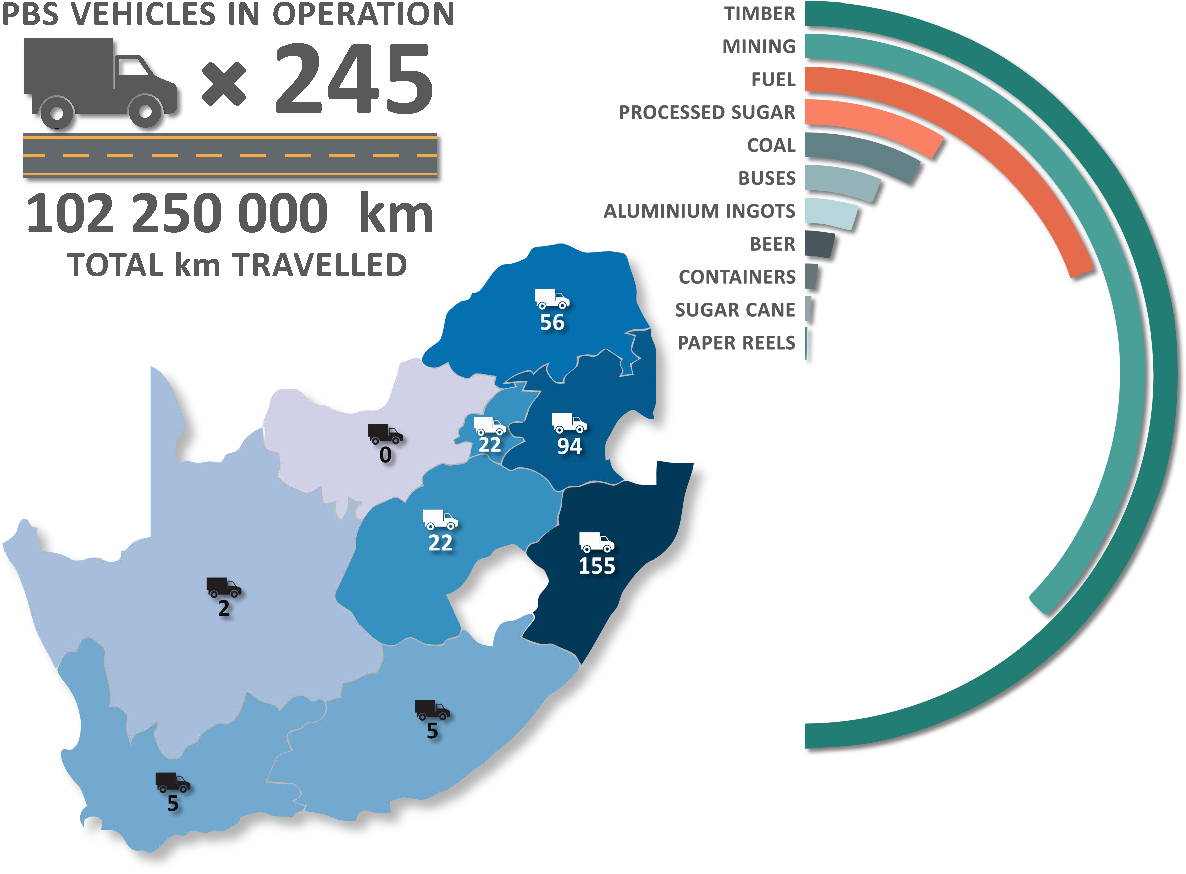
\includegraphics[width=1\textwidth]{fig/pbs-pilot_vehicles-and-commodities-june-2017}
        \caption{Summary of operating PBS vehicles and commodities in South Africa as of June 2017 \cite{Nordengen2018}}
        \label{figure:summary-of-operating-pbs-vehicles-and-commodities-in-south-africa-june-2017}
    \end{figure}
%----------------------------------------------
%      FIGURE
%----------------------------------------------

    The monitoring data that has been collected and analysed for the duration of the PBS pilot project shows PBS vehicles require fewer trips to transport the same amount of payload which leads to reductions in fuel usage and CO\textsubscript{2} emissions. PBS vehicles are recorded to have a 39\% reduction in accidents relative to their baseline equivalents. This highlights the improved safety performance of the PBS vehicles. The monitoring data shows that the PBS vehicles operating as of June 2017 were saving 74067 trips per year which resulted in R~26.64 million of fuel saved and a reduction of 6246 tons of CO\textsubscript{2}. Each \gls{pbs} vehicle saves R~24448 in road wear per vehicle per year and \gls{pbs} vehicles have a 39\% reduction in accidents relative to their baseline equivalents (see Figure~\ref{figure:summary-of-pbs-monitoring-data-june-2017}).

%----------------------------------------------
%      FIGURE
%----------------------------------------------
    \begin{figure}
        \centering
        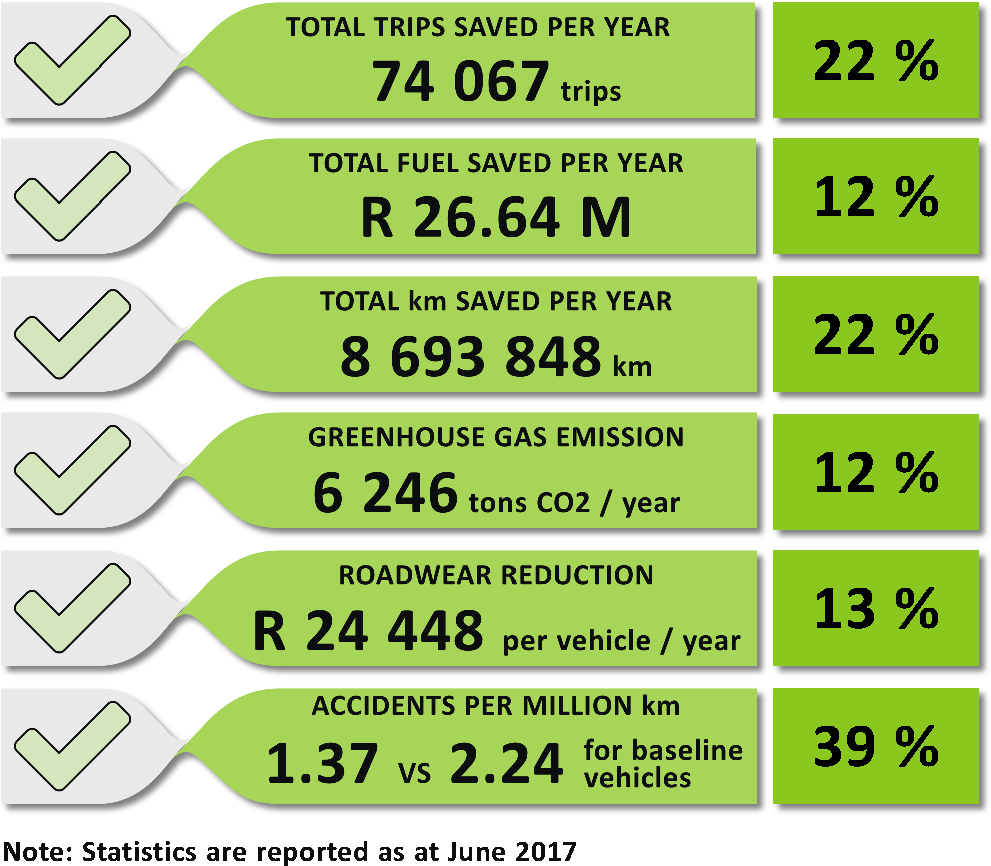
\includegraphics[width=1\textwidth]{fig/pbs-pilot_yearly-statistics-june-2017}
        \caption{Summary of PBS monitoring data as of June 2017 \cite{Nordengen2018}}
        \label{figure:summary-of-pbs-monitoring-data-june-2017}
    \end{figure}
%----------------------------------------------
%      FIGURE
%----------------------------------------------

  The benefits realised by the small sample of \gls{pbs} vehicles is clear. Increasing participation in the \gls{pbs} project will improve the productivity of the South African logistics, decrease the environmental impact of transport operations and reduce damage to infrastructure. Thus, it is beneficial to make the \gls{pbs} assessment process as attractive and efficient as possible to motivate more parties to participate.

%==============================================
%      SECTION
%==============================================
\section{Towards Quicker PBS Assessments}\label{section:towards-quicker-pbs-assessments}

The process of performing a \gls{pbs} assessment requires accurate vehicle details to be sourced from \glspl{oem}, the expertise to interpret the information and tools to perform the assessment. The multi-body vehicle dynamics packages required to simulate vehicle performance are expensive, require know-how to correctly build a representative vehicle model and require a significant amount of computational power to operate. 

This leads to a lengthy and computationally expensive process that requires input from multiple experts. Studies that have been done to simplify and speed up the assessment process are explored in this section.

%      SUBSECTION
%----------------------------------------------
\subsection{Pro-forma Design}\label{section:pro-forma-design}

  De Pont~\cite{Pont2010} initially introduced the concept of pro-forma designs to alleviate time and cost constraints of a PBS assessment. The pro-forma design methodology sets geometrical constraints for a vehicle combination that when used in the design of a vehicle ensures satisfactory low-speed directional \gls{pbs} performance (\gls{fs}, \gls{ts}, \gls{lssp}) eliminating the need for futher low-speed performance testing. 
  
  De pont generated geometrical constraints for three typical heavy vehicle configurations in New Zealand (truck and full trailer, truck and simple trailer and B-double) by performing a parametric sensitivity analysis on the effect of key \gls{hcv} geometrical parameters on their low-speed \gls{pbs} performance using the yaw/roll multi-body vehicle dynamics package developed by \gls{umtri} . This resulted in diagrams indicating the range within which key dimensional parameters could be varied while achieving the required PBS safety performance.
  
  Benade extended the pro-forma design concept to car-carriers in South Africa by Benade et al. \cite{Benade2015}. To enable rapid evaluation of low-speed vehicle performance, he made use of a \gls{lsmm} developed by de~Saxe~\cite{DeSaxe2012}  which was shown to correlate well with vehicle performance evaluated with \trucksim{} while obtaining solution speed improvements of between 261\% and 546\%.
  
  Benade et al. developed the pro-forma constraints by performing a sensitivity analysis of each of the critical parameters affecting low-speed vehicle performance. Each parameter was varied up and down in increments of 10\% (or increments of 1 for certain parameters such as number of steer axles) to develop upper and lower constraints. \matlab{} code developed by Benade et al. was used to generate 10 000 vehicle configurations satisfying the generated constraints. The low-speed \gls{pbs} performance of the generated combinations was then evaluated using the LSMM and it was found that all of them achieved Level 1 \gls{pbs} performance requirements.

  Benade et al. found that making effective use of the pro-forma design method could lead to reducing the cost of \gls{pbs} assessments by an estimated 1.2~million rand \cite{Benade2015} per year. However in its current form it is limited as it only ensures compliance with Level~1 low-speed \gls{pbs} performance measures and further work would need to be performed to ensure compliance with the high-speed \gls{pbs} performance measures.

  A similar pro-forma approach has been developed by the \gls{nhvr} who made blueprint designs for a variety of truck configurations publicly available on their website~\cite{NationalHeavyVehicleRegulator}. Blueprint \gls{hcv} configurations have been pre-approved by the NHVR and designs based on these configurations will shorten the lead time in the PBS approval process.

  %      SUBSECTION
  %----------------------------------------------
\subsection{Predicting PBS Performance}\label{section:optimisation-of-vehicles-within-the-pbs-framework}

Dessein~\cite{Dessein2012} explored consideration of the PBS framework prior to the detail design phase through optimisation of \gls{hcv} design within the \gls{pbs} framework. Simplified models for eight performance measures (\gls{srt}, \gls{ra}, \gls{lssp}, \gls{fs}, \gls{ts}, \gls{sta}, \gls{graa}) were used to estimate the \gls{hcv} performance. Limiting the number of performance measures evaluated allowed the calculations to be automated by using a sequential quadratic programming algorithm within MATLAB.

The routine varied the five vehicle parameters listed for four types of vehicle (A-Double, B-Double, truck and pig trailer, truck and dog trailer):

\begin{itemize}
    \item Number of axles in each axle group
    \item Wheelbases of all vehicle units
    \item Hitch offset
    \item Payload (size/location/density)
\end{itemize}

The optimisation routine considered a Level~2 PBS requirement, and the vehicle configuration yielding the highest payload (and hence highest productivity) was chosen as optimal. The optimised vehicles were compared to those designed using prescriptive methods.

It was discovered that the vehicles designed using a prescriptive approach were in fact more productive than the PBS equivalent for payloads with a density lower than 400 kg/m\ssth{}. This suggests that an optimisation approach would be very useful in evaluating whether a vehicle can be designed to be more productive using the PBS approach; potentially preventing a costly, unsuccessful, iterative design process.

Dessein showed that the prescriptive vehicles failed to meet the PBS Level~2 \gls{srt} requirement of 0.35~g for most payload densities. Dessein highlighted one of the major disadvantages of the prescriptive approach in that it does not directly consider the vehicles safety performance but imposes only geometrical and mass constraints. Importantly, there is an opportunity using the PBS approach to increase safety and reduce road fatalities even if at the lower payload densities there is little scope to increase the vehicle productivity.

The results of the \gls{adr} developed by Dessein indicated that there is a potential for determining an estimated productivity gain of a PBS assessment before detailed design begins. It can also yield optimal \gls{hcv} configurations that can be used as a starting point in the detailed design of the \gls{hcv}, speeding the process up and increasing the probability of PBS approval.

%      SUBSECTION
%----------------------------------------------
\subsection{Machine Learning Models}\label{section:machine-learning models}

Berman et al. \cite{Berman2015} developed a lightweight tool requiring only vehicle geometry to predict the low-speed \gls{pbs} performance measures of a B-double combination. In total 22 input parameters were randomly selected to conduct 10 000 simulations on a B-double. Supervised machine learning techniques were used to develop a model to predict \gls{lssp}, \gls{fs}, \gls{mod}, \gls{dom} and \gls{ts} performance measures from the simulated data. The model provides an accessible way for \glspl{oem} to quickly and accurately evaluate the low-speed PBS performance of their vehicle before a formal PBS assessment without the need for extensive mechanical knowledge of multi-body vehicle dynamics systems using only geometric parameters of the vehicle combination.

Following his initial research, Berman et al. \cite{Berman2016} developed a lightweight prediction tool using neural networks to predict the high-speed performance of a 9-axle B-double combination. Upper and lower bounds were selected for 30 unique input parameters defining the vehicle geometry, payload and suspension. 36 470 vehicle configurations were created using random sampling within the range of each input parameter assuming a uniform distribution. The model can rapidly predict the \gls{hsto}, \gls{srt}, \gls{tasp}, \gls{ra} and \gls{ydc} PBS performance of a 9-axle B-double combination as well as overall \gls{pbs} performance with a high level of accuracy. The model is intended for determining preliminary PBS performance of a vehicle combination as a guide for \glspl{oem} and transport regulators as a precursor to a formal PBS assessment.

%==============================================
%      SECTION
%==============================================
\section{Design Parameter Effect on Vehicle Performance}\label{section:design-parameter-effect-on-vehicle-performance}
The following Section discusses previous studies that have focused on determining the influence of \gls{hcv} design parameters on heavy vehicle safety.

%      SUBSECTION
%----------------------------------------------
\subsection{Influence of Heavy Vehicle Design Parameters on Vehicle Performance}\label{section:australian-study-on-the-influence-of-heavy-vehicle-design-parameters}

Prem et al. \cite{Prem2002} conducted a study on the Australian heavy vehicle fleet to determine the influence of various design parameters on vehicle safety as assessed using the PBS framework. A baseline configuration was chosen for a variety of vehicle configurations. The design parameters were then varied by +/-20\% and the effects on each performance measure were tabulated, indicating the influence of each performance measure using a scale with 4 discrete quantifiers (++, + for improved performance and - -, - for degraded performance). The results of this study are summarised in Table \ref{table:influence-of-design-features-performance-characteristics-of-australian-fleet}.

%----------------------------------------------
%      TABLE
%----------------------------------------------
\begin{table}[H]
    \centering\scriptsize
    \begin{threeparttable}
        \caption{Influence of design features and broad summary of parametric effects \cite{Prem2002}}
        \begin{tabulary}{\textwidth}{|L|c|c|c|c|c|c|c|c|c|c|c|c|c|c|c|}
        \toprule
            \multicolumn{1}{l}{\textbf{Performance measure}} & \multicolumn{1}{l}{\begin{sideways}\textbf{Increase Engine Power/Torque}\end{sideways}} & \multicolumn{1}{l}{\begin{sideways}\textbf{Increase Driveline Gear Ratio}\end{sideways}} & \multicolumn{1}{l}{\begin{sideways}\textbf{Increase CG Height}\end{sideways}} & \multicolumn{1}{l}{\begin{sideways}\textbf{Increase Axle Loads}\end{sideways}} & \multicolumn{1}{l}{\begin{sideways}\textbf{Longer Prime Mover Wheelbase}\end{sideways}} & \multicolumn{1}{l}{\begin{sideways}\textbf{Longer Trailer Wheelbase}\end{sideways}} & \multicolumn{1}{l}{\begin{sideways}\textbf{Longer Dolly Wheelbase}\end{sideways}} & \multicolumn{1}{l}{\begin{sideways}\textbf{Increase Number of Articulation Points}\end{sideways}} & \multicolumn{1}{l}{\begin{sideways}\textbf{Increase Axle Group Spread}\end{sideways}} & \multicolumn{1}{l}{\begin{sideways}\textbf{Increase Coupling Rear Overhang}\end{sideways}} & \multicolumn{1}{l}{\begin{sideways}\textbf{Increase Suspension Roll Stiffness}\end{sideways}} & \multicolumn{1}{l}{\begin{sideways}\textbf{Increase Tyre Cornering Stiffness}\end{sideways}} & \multicolumn{1}{l}{\begin{sideways}\textbf{Increase Front Overhang}\end{sideways}} & \multicolumn{1}{l}{\begin{sideways}\textbf{Increase Rear Overhang}\end{sideways}} & \multicolumn{1}{l}{\begin{sideways}\textbf{Decrease Speed}\end{sideways}} \bigstrut\\
            \hline
            Startability &       & ++    &       & - -    &       &       &       &       &       &       &       &       &       &       &  \bigstrut\\
            \hline
            Gradeability A & ++    & ++    &       & - -    &       &       &       &       &       &       &       &       &       &       &  \bigstrut\\
            \hline
            Gradeability B & ++    & +/-   &       & -     &       &       &       &       &       &       &       &       &       &       &  \bigstrut\\
            \hline
            Acceleration Capability & +     & -     &       & -     &       &       &       &       &       &       &       &       &       &       & + \bigstrut\\
            \hline
            Tracking Ability on a Straight Path &       &       & - -    & - -    & -     & -     & -     & -     & +     & -     & +     & ++    &       &       & ++ \bigstrut\\
            \hline
            Low-speed Offtracking &       &       &       &       & - -    & - -    & -     & ++    &       & +     &       &       & -     &       &  \bigstrut\\
            \hline
            Frontal Swing &       &       &       &       & - -    &       &       &       &       &       &       &       & - -    &       &  \bigstrut\\
            \hline
            Tail Swing &       &       &       &       &       & +     &       &       &       &       &       &       &       & - -    &  \bigstrut\\
            \hline
            Steer Tyre Friction Demand &       &       &       &       & ++    &       &       &       & - -    &       &       &       &       &       &  \bigstrut\\
            \hline
            Static Rollover Threshold &       &       & - -    & -     &       &       &       &       &       &       & +     &       &       &       &  \bigstrut\\
            \hline
            Rearward Amplification &       &       & -     & -     & +     & ++    & +     & - -    & +     & -     & +     & ++    &       &       & ++ \bigstrut\\
            \hline
            High-speed Transient Offtracking &       &       & - -    & - -    & +     & ++    &       &       & +     & -     &       & ++    &       &       & ++ \bigstrut\\
            \hline
            Yaw Damping Coefficient &       &       & - -    &       &       & ++    &       &       & +     &       &       & ++    &       &       & ++ \bigstrut\\
            \hline
            GM per SAR &       &       &       & -     &       &       &       &       &       &       &       &       &       &       &  \bigstrut\\
            \hline
            Horizontal Tyre Forces & - -    &       &       & - -    &       &       &       &       & - -    &       &       &       &       &       &  \bigstrut\\
            \hline
            Max. Effect Relative to Ref. Vehicles &       &       &       & - -    & ++    & ++    & +     &       & +     &       &       &       &       &       &  \bigstrut\\
            \hline
        \end{tabulary}%
        \label{table:influence-of-design-features-performance-characteristics-of-australian-fleet}
        %Enter table label for referencing here
        \begin{tablenotes}
            \item[1] ++ Significant positive effect on performance
            \item[2] + Moderate positive effect
            \item[3] \textit{blank} Little or no influence
            \item[4] - Moderate negative effect
            \item[5] - - Significant negative effect
        \end{tablenotes}
    \end{threeparttable}
\end{table}%
%----------------------------------------------
%      TABLE
%----------------------------------------------

The results of the study conducted by Prem et al. provide useful insight into how the design parameters effect each performance measure within a range of 20\% of the baseline design parameters. The design parameters of a heavy vehicle are often constrained due to manufacturing limitations and regulations that need to be adhered to. A design parameter could heavily influence the performance of a heavy vehicle; however, it may not be possible to alter that parameter due to design and legal constraints. On the other hand, a parameter may have little effect on the vehicle safety performance but be able to be varied within a large range. The study considered a wide range of vehicle configurations and lumped the results of each vehicle into one summarised result. This loses any insights into how the effect of changing certain design parameters may differ between the vehicle configurations.

%      SUBSECTION
%----------------------------------------------
\subsection{The UMTRI Component Factbook}\label{section:umtri-component-factbook}

Fancher et al. at \gls{umtri} compiled a comprehensive document in 1986 detailing the mechanical properties of components used in heavy vehicles, their influences on manoeuvring performance and a collection of parametric data from the United States heavy vehicle fleet \cite{Fancher1986}. The mechanical properties discussed were categorised as follows:

\begin{enumerate}
    \item Geometric layout
    \item Mass distribution
    \item Tyres
    \item Suspensions
    \item Steering systems
    \item Brakes
    \item Frames
    \item Hitches
\end{enumerate}

In each category, the effect of the mechanical properties on vehicle performance was discussed. A summary of the effect of each mechanical property considered is included in Tables \ref{table:effect-of-the-mechanical-properties-of-tyres-on-vehicle-dynamic-performance} to \ref{table:effect-of-the-mechanical-properties-of-mass-distribution-on-vehicle-dynamic-performance}. Steering systems, frames and braking are beyond the scope of this dissertation, however their effects on vehicle dynamic performance are included for completeness and the interest of the reader.

%----------------------------------------------
%      TABLE
%----------------------------------------------
\begin{table}[H]
	\centering\footnotesize
	\begin{threeparttable}
	
        \begin{tabulary}{\textwidth}{lcccccccccc}
            \toprule
            \textbf{Pertinent Mechanical Property} & \begin{sideways}\textbf{Low-speed tracking}\end{sideways} & \begin{sideways}\textbf{Hi-speed tracking}\end{sideways} & \begin{sideways}\textbf{Roll stability}\end{sideways} & \begin{sideways}\textbf{Handling stability}\end{sideways} & \begin{sideways}\textbf{Response time}\end{sideways} & \begin{sideways}\textbf{Rearward amplification}\end{sideways} & \begin{sideways}\textbf{Braking efficiency}\end{sideways} & \begin{sideways}\textbf{Transient braking \& turning}\end{sideways} & \begin{sideways}\textbf{Downhill braking}\end{sideways} & \begin{sideways}\textbf{Response to disturbances}\end{sideways} \\\midrule
            Cornering coefficient $C_{alpha}/F_z$ & -     & Hi    & -     & Hi    & Hi    & Hi    & -     & Hi    & -     & Hi \\
            Curvature in $C_{alpha}$ ($C_{alpha}$ vs Vertical Load) & Low   & -     & -     & Hi    & Low   & Low   & -     & -     & -     & - \\
            Aligning stiffness (pneumatic trail) & -     & -     & -     & Low   & -     & -     & -     & -     & -     & - \\
            Vertical stiffness & -     & -     & Med   & -     & -     & -     & -     & -     & -     & - \\
            Peak friction, $m_p$ & -     & -     & -     & -     & -     & -     & Hi    & Hi    & -     & - \\
            Sliding friction, $m_s$ & -     & -     & -     & -     & -     & -     & -     & Med   & -     & - \\
            Long./Lat Interaction & -     & -     & -     & -     & -     & -     & -     & Med   & -     & - \\
            \bottomrule
		\end{tabulary}

		\caption{Effect of the mechanical properties of tyres on vehicle dynamic performance \cite{Fancher1986}}
		\label{table:effect-of-the-mechanical-properties-of-tyres-on-vehicle-dynamic-performance}

	\end{threeparttable}
\end{table}
%----------------------------------------------
%      TABLE
%----------------------------------------------

%----------------------------------------------
%      TABLE
%----------------------------------------------
\begin{table}[H]
	\centering\footnotesize
	\begin{threeparttable}
	
        \begin{tabulary}{\textwidth}{lcccccccccc}
            \toprule
            \textbf{Pertinent Mechanical Property} & \begin{sideways}\textbf{Low-speed tracking}\end{sideways} & \begin{sideways}\textbf{Hi-speed tracking}\end{sideways} & \begin{sideways}\textbf{Roll stability}\end{sideways} & \begin{sideways}\textbf{Yaw stability}\end{sideways} & \begin{sideways}\textbf{Response time}\end{sideways} & \begin{sideways}\textbf{Rearward amplification}\end{sideways} & \begin{sideways}\textbf{Braking efficiency}\end{sideways} & \begin{sideways}\textbf{Transient braking}\end{sideways} & \begin{sideways}\textbf{Downhill braking}\end{sideways} & \begin{sideways}\textbf{Response to disturbances}\end{sideways} \\\midrule
            Vertical stiffness & -     & -     & -     & -     & -     & -     & -     & Med   & -     & - \\
            Roll stiffness & -     & Med   & Hi    & Hi    & Hi    & Hi    & -     & -     & -     & Med \\
            Roll centre height & -     & Med   & Hi    & Hi    & Hi    & Hi    & -     & -     & -     & Med \\
            Damping & -     & -     & -     & -     & Med   & Med   & -     & Low   & -     & Low \\
            Roll steer & -     & Low   & -     & Low   & Low   & Low   & -     & -     & -     & Low \\
            Compliance steer & -     & Low   & -     & Low   & Low   & Low   & -     & -     & -     & Low \\
            Interaxle load transfer & -     & -     & -     & -     & -     & -     & Hi    & -     & -     & -\\
            \bottomrule
		\end{tabulary}

		\caption{Effect of the mechanical properties of suspension systems on vehicle dynamic performance \cite{Fancher1986}}
		\label{table:effect-of-the-mechanical-properties-of-suspensions-on-vehicle-dynamic-performance}

	\end{threeparttable}
\end{table}
%----------------------------------------------
%      TABLE
%----------------------------------------------

%----------------------------------------------
%      TABLE
%----------------------------------------------
\begin{table}[H]
	\centering\footnotesize
	\begin{threeparttable}
	
        \begin{tabulary}{\textwidth}{lcccccccccc}
            \toprule
            \textbf{Pertinent Mechanical Property} & \begin{sideways}\textbf{Low-speed tracking}\end{sideways} & \begin{sideways}\textbf{Hi-speed tracking}\end{sideways} & \begin{sideways}\textbf{Roll stability}\end{sideways} & \begin{sideways}\textbf{Yaw stability}\end{sideways} & \begin{sideways}\textbf{Response time}\end{sideways} & \begin{sideways}\textbf{Rearward amplification}\end{sideways} & \begin{sideways}\textbf{Braking efficiency}\end{sideways} & \begin{sideways}\textbf{Transient braking}\end{sideways} & \begin{sideways}\textbf{Downhill braking}\end{sideways} & \begin{sideways}\textbf{Response to disturbances}\end{sideways} \\\midrule
            Roll steer & -     & -     & -     & Low   & -     & -     & -     & -     & -     & - \\
            Lateral force compliance steer & -     & -     & -     & Hi    & -     & -     & -     & -     & -     & - \\
            Brake steer & -     & -     & -     & -     & -     & -     & -     & Med   & -     & Hi \\
            Gear Ratio & -     & -     & -     & -     & -     & -     & -     & -     & -     & -\\
            \bottomrule
		\end{tabulary}

		\caption{Effect of the mechanical properties of steering systems on vehicle dynamic performance \cite{Fancher1986}}
		\label{table:effect-of-the-mechanical-properties-of-steering-systems-on-vehicle-dynamic-performance}

	\end{threeparttable}
\end{table}
%----------------------------------------------
%      TABLE
%----------------------------------------------

%----------------------------------------------
%      TABLE
%----------------------------------------------
\begin{table}[H]
	\centering\footnotesize
	\begin{threeparttable}
	
        \begin{tabulary}{\textwidth}{lccc}
            \toprule
            \textbf{Pertinent Mechanical Property} & \begin{sideways}\textbf{Constant deceleration braking}\end{sideways} & \begin{sideways}\textbf{Braking while turning}\end{sideways} & \begin{sideways}\textbf{Mountain descents}\end{sideways} \\\midrule
            Effectiveness & Hi    & Hi    & Hi\tnote{1} \\
            Torque rise and fall characteristics & -     & Hi    & - \\
            Thermal capacity and cooling & -     & -     & Hi\\
            \bottomrule
		\end{tabulary}

		\caption{Effect of the mechanical properties of brakes on vehicle dynamic performance \cite{Fancher1986}}
        \label{table:effect-of-the-mechanical-properties-of-brakes-on-vehicle-dynamic-performance}
        
        \begin{tablenotes}
            \item[1] Effect could be high
        \end{tablenotes}

	\end{threeparttable}
\end{table}
%----------------------------------------------
%      TABLE
%----------------------------------------------

%----------------------------------------------
%      TABLE
%----------------------------------------------
\begin{table}[H]
	\centering\footnotesize
	\begin{threeparttable}
	
        \begin{tabulary}{\textwidth}{lcccccccccc}
            \toprule
            \textbf{Pertinent Mechanical Property} & \begin{sideways}\textbf{Low-speed tracking}\end{sideways} & \begin{sideways}\textbf{Hi-speed tracking}\end{sideways} & \begin{sideways}\textbf{Roll stability}\end{sideways} & \begin{sideways}\textbf{Yaw stability}\end{sideways} & \begin{sideways}\textbf{Response time}\end{sideways} & \begin{sideways}\textbf{Rearward amplification}\end{sideways} & \begin{sideways}\textbf{Braking efficiency}\end{sideways} & \begin{sideways}\textbf{Transient braking}\end{sideways} & \begin{sideways}\textbf{Downhill braking}\end{sideways} & \begin{sideways}\textbf{Response to disturbances}\end{sideways} \\\midrule
            Torsional stiffness & Low   & Low   & -     & Low   & -     & -     & -     & Low   & -     & -\\
            \bottomrule
		\end{tabulary}

		\caption{Effect of the mechanical properties of frames on vehicle dynamic performance \cite{Fancher1986}}
		\label{table:effect-of-the-mechanical-properties-of-frames-on-vehicle-dynamic-performance}

	\end{threeparttable}
\end{table}
%----------------------------------------------
%      TABLE
%----------------------------------------------

%----------------------------------------------
%      TABLE
%----------------------------------------------
\begin{table}[H]
	\centering\footnotesize
	\begin{threeparttable}
	
        \begin{tabulary}{\textwidth}{lccccccccc}
            \toprule
            \textbf{Pertinent Mechanical Property} & \begin{sideways}\textbf{Low-speed tracking}\end{sideways} & \begin{sideways}\textbf{Hi-speed tracking}\end{sideways} & \begin{sideways}\textbf{Roll stability}\end{sideways} & \begin{sideways}\textbf{Yaw stability}\end{sideways} & \begin{sideways}\textbf{Response time}\end{sideways} & \begin{sideways}\textbf{Rearward amplification}\end{sideways} & \begin{sideways}\textbf{Braking efficiency}\end{sideways} & \begin{sideways}\textbf{Transient braking}\end{sideways} & \begin{sideways}\textbf{Downhill braking}\end{sideways} \\
            \midrule
            Wheelbase - truck/tractor & Med   & Low   & -     & Med   & Med   & -     & Low   & Low   & - \\
            Wheelbase - trailer & Hi    & Hi    & -     & -     & Med   & Hi    & Low   & -     & - \\
            Wheelbase - dolly & Med   & Med   & -     & -     & -     & Med   & Low   & -     & - \\
            Track width & -     & -     & Hi    & Med   & -     & -     & -     & Med   & - \\
            Fifth wheel offset - tractors & Low   & -     & Low   & Low   & -     & -     & Med   & Med   & - \\
            Pintle overhang - trucks \& trailers & Low   & Low   & -     & -     & -     & Hi    & -     & -     & - \\
            Fifth wheel height - tractor & -     & -     & Low   & -     & -     & -     & Low   & -     & -\\
            \bottomrule
		\end{tabulary}

		\caption{Effect of the mechanical properties of the geometric layout on vehicle dynamic performance \cite{Fancher1986}}
		\label{table:effect-of-the-mechanical-properties-of-geometric-layout-on-vehicle-dynamic-performance}

	\end{threeparttable}
\end{table}
%----------------------------------------------
%      TABLE
%----------------------------------------------

%----------------------------------------------
%      TABLE
%----------------------------------------------
\begin{table}[H]
	\centering\footnotesize
	\begin{threeparttable}
	
        \begin{tabulary}{\textwidth}{lcccccccccc}
            \toprule
            \textbf{Pertinent Mass Distribution} & \begin{sideways}\textbf{Low-speed tracking}\end{sideways} & \begin{sideways}\textbf{Hi-speed tracking}\end{sideways} & \begin{sideways}\textbf{Roll stability}\end{sideways} & \begin{sideways}\textbf{Yaw stability}\end{sideways} & \begin{sideways}\textbf{Response time}\end{sideways} & \begin{sideways}\textbf{Rearward amplification}\end{sideways} & \begin{sideways}\textbf{Braking efficiency}\end{sideways} & \begin{sideways}\textbf{Transient braking}\end{sideways} & \begin{sideways}\textbf{Downhill braking}\end{sideways} & \begin{sideways}\textbf{Response to disturbances}\end{sideways} \\\midrule
            Weight & -     & Hi    & Hi    & Hi    & Hi    & Hi    & Hi    & Hi    & Hi    & Hi \\
            CG height & -     & -     & Hi    & Hi    & Low   & Hi    & Med   & Med   & -     & Low \\
            Fore-aft CG location & -     & Hi    & Med   & Hi    & Hi    & Hi    & Hi    & Hi    & -     & Hi \\
            Yaw moment of inertia & -     & -     & -     & -     & Hi    & Med   & -     & Low   & -     & Low \\
            Pitch moment of inertia & -     & -     & -     & -     & -     & -     & -     & Med   & -     & - \\
            Sprung roll moment of inertia & -     & -     & Med   & -     & Low   & Low   & -     & Low   & -     & Low\\
            \bottomrule
		\end{tabulary}

		\caption{Effect of the mechanical properties of the mass distribution on vehicle dynamic performance \cite{Fancher1986}}
		\label{table:effect-of-the-mechanical-properties-of-mass-distribution-on-vehicle-dynamic-performance}

	\end{threeparttable}
\end{table}
%----------------------------------------------
%      TABLE
%----------------------------------------------

%==============================================
%      SECTION
%==============================================
\section{Collections of Heavy Vehicle Design Parameters}\label{section:collections-of-heavy-vehicle-design-parameters}
Heavy vehicle design parameters are well documented for overseas vehicles (US and Canada), however there have been limited studies conducted in South Africa with the intention of cataloguing the mechanical properties of heavy vehicle components.

Fancher et al. \cite{Fancher1986} summarised heavy vehicle design parameters for the US heavy vehicle fleet in the component Factbook mentioned in Section~\ref{section:umtri-component-factbook}. This data was collected in 1986 and is outdated, however is still a useful source to estimate approximate vehicle design parameters.

A more recent collection of heavy vehicle design parameters collected in 2003 is included in a review of truck characteristics performed by Harwood et al. \cite{Harwood2003} as part of the \gls{nchrp} with the intention of using this information to better guide the design of roadways.

Additional resources for heavy vehicle design parameters and their influence on heavy vehicle performance include studies conducted by Ervin et al. \cite{Ervin1986} and Winkler et al. \cite{Winkler1995}, \cite{Winkler2011}.

%==============================================
%      SECTION
%==============================================
\section{Significance of This Research}\label{section:significance-of-this-research}
The review of the literature presented in Sections \ref{section:performance-based-standards} to \ref{section:collections-of-heavy-vehicle-design-parameters} highlights the significance of this research:

\begin{enumerate}
\item Published studies have looked at \gls{vdp} influence on vehicle performance by varying a limited number of parameters within set percentage range of values without considering allowable ranges within which each design parameter could be varied. This presents a gap in current research to evaluate the effect of a larger number of \gls{vdp} on overall vehicle performance based on allowable ranges within which \gls{vdp} could be varied based on physical, legal and OEM imposed constraints.
\item Research exists to show how \glspl{vdp} affect vehicle performance. To some extent this can be used as a guide to determine if a design parameter should be included in a vehicle performance model. There is however a lack of research investigating the relative effect of each \glspl{vdp} making up a multi-body vehicle dynamics model on vehicle performance within the \gls{pbs} framework.
\item Performing \gls{pbs} assessments is a costly and time consuming exercise. \gls{oem} data needs to be collected to define the mechanical properties of each vehicle unit within the combination being assessed to ensure that a model representative of the actual vehicle is built, resulting in accurate evaluation of vehicle performance within the \gls{pbs} framework. Red-tape can often slow the process and should certain parameters not be available, conservative estimates need to be made to ensure on-road performance will at the very least be as good as that predicted by the \gls{pbs} assessment. Evaluating the relative influence of each \gls{vdp} required for a multi-body vehicle dynamics model will yield insight as to the \glspl{vdp} that have little influence on vehicle performance and can be safely estimated while still simulating representative vehicle performance.
\end{enumerate}
\chapter{Objectives}\label{section:objectives}

The objectives of this MSc dissertation are as follows:

\begin{enumerate}
\item Quantify the relative effect of pertinent \glspl{vdp} of a multi-body vehicle dynamics model on the vehicle safety as measured using the \gls{pbs} framework currently being used in South Africa for three commonly used \gls{hcv} designs.
\item Develop easy-to-use look-up tables displaying the relative effect of each of the evaluated \glspl{vdp} on each of the \gls{pbs} performance measures for vehicle designers and \gls{pbs} assessors to use in vehicle design, optimisation and \gls{pbs} vehicle data acquisition.
\item Highlight interesting observations from the results and discuss their implications for the \gls{pbs} initiative in South Africa and globally.
\end{enumerate}

Achieving these objectives is important as it will provide guidance as to which \glspl{vdp} can be safely estimated in the absence of definitive data when evaluating the \gls{pbs} performance of a \gls{hcv} and provide guidance as to the critical \glspl{vdp} which need to be accurately estimated to predict representative vehicle safety of a \gls{hcv}. Furthermore, it will provide insight into which \glspl{vdp} should be focused on when attempting to improve a vehicles performance for a performance measure within the \gls{pbs} framework.
\chapter{Methodology}\label{chapter:methodology}
A high-level overview of the study performed on the relative effect of the \glspl{vdp} of \glspl{hcv} is as follows:

\begin{enumerate}\addtolength{\itemsep}{0.5\baselineskip}
\item Develop a set of baseline combinations to represent a range of highly productive \glspl{hcv}.
\item Define reasonable ranges for each pertinent \gls{vdp} to be varied within.
\item Evaluate the relative effect of altering each \gls{vdp} within its selected range on overall vehicle performance within the \gls{pbs} framework.
\end{enumerate}

%==============================================
%      SECTION
%==============================================
\section{Baseline Combinations\label{section:methodbaselinecombinations}}
Three baseline \gls{hcv} configurations were developed based on South African workhorse vehicles and Australia's most common PBS vehicle.  Previous \gls{pbs} assessments conducted by \gls{wits} and the \gls{csir} were used to develop the design of each of the baseline combinations.

The same high-level prime mover was used for each baseline, with adjustments to the wheelbase where necessary. A set of representative suspensions were developed and used for all combinations to avoid inserting any bias from discrepancies between the baseline suspension designs. Sections \ref{section:baseline-quad-semi} to \ref{section:baseline-rigid-drawbar-combination} detail the development of each baseline vehicle configuration.

%==============================================
%      SECTION
%==============================================
\section{\gls{vdp} ranges\label{section:methodvdpranges}}
To define reasonable upper and lower limits for each pertinent \gls{vdp}, \gls{oem} variations, legal restrictions, physical constraints, global studies, and data from \gls{pbs} assessments previously conducted by Wits were consolidated and consulted. Details on how the range for each pertinent \gls{vdp} was chosen are contained in Section~\ref{chapter:parameter-range-selection}.

The geometrical limits of a \gls{hcv} are largely governed by the prescriptive legislation of the country in which the combination will be operating.The South African legislation was chosen for developing the geometrical limits to provide value to the \gls{pbs} pilot project in South African. This would not limit the results to being applicable only in South Africa, but if used internationally, the local legislation should be consulted to determine where results may differ.

Inertial, suspension and tyre properties are not widely available which is one of the factors that drive the need for this research. \gls{oem} variations, data from PBS assessments conducted by Wits and Global studies were consulted and the information was consolidated to develop ranges for each of the pertinent \glspl{vdp} that would represent the global \gls{hcv} fleet as local legislation does not dictate any restrictions on the origins of \gls{hcv} components.

%==============================================
%      SECTION
%==============================================
\section{Evaluating \gls{vdp} Relative Influence}

To evaluate the relative influence of each \gls{vdp} on each of the baseline combinations, the \glspl{vdp} were varied in isolation while keeping all other \glspl{vdp} constant at their baseline value. To evaluate the influence of each \gls{vdp}, the \gls{vdp} was varied by 5 evenly distributed points from its maximum to minimum value within its range as determined in Section~\ref{chapter:parameter-range-selection}. This resulted in a total of 8345 simulations being run in \trucksim{} as illustrated in Figure~\ref{figure:number-of-simulations-overview}.

%----------------------------------------------
%      FIGURE
%----------------------------------------------
\begin{figure}[H]
	\centering
	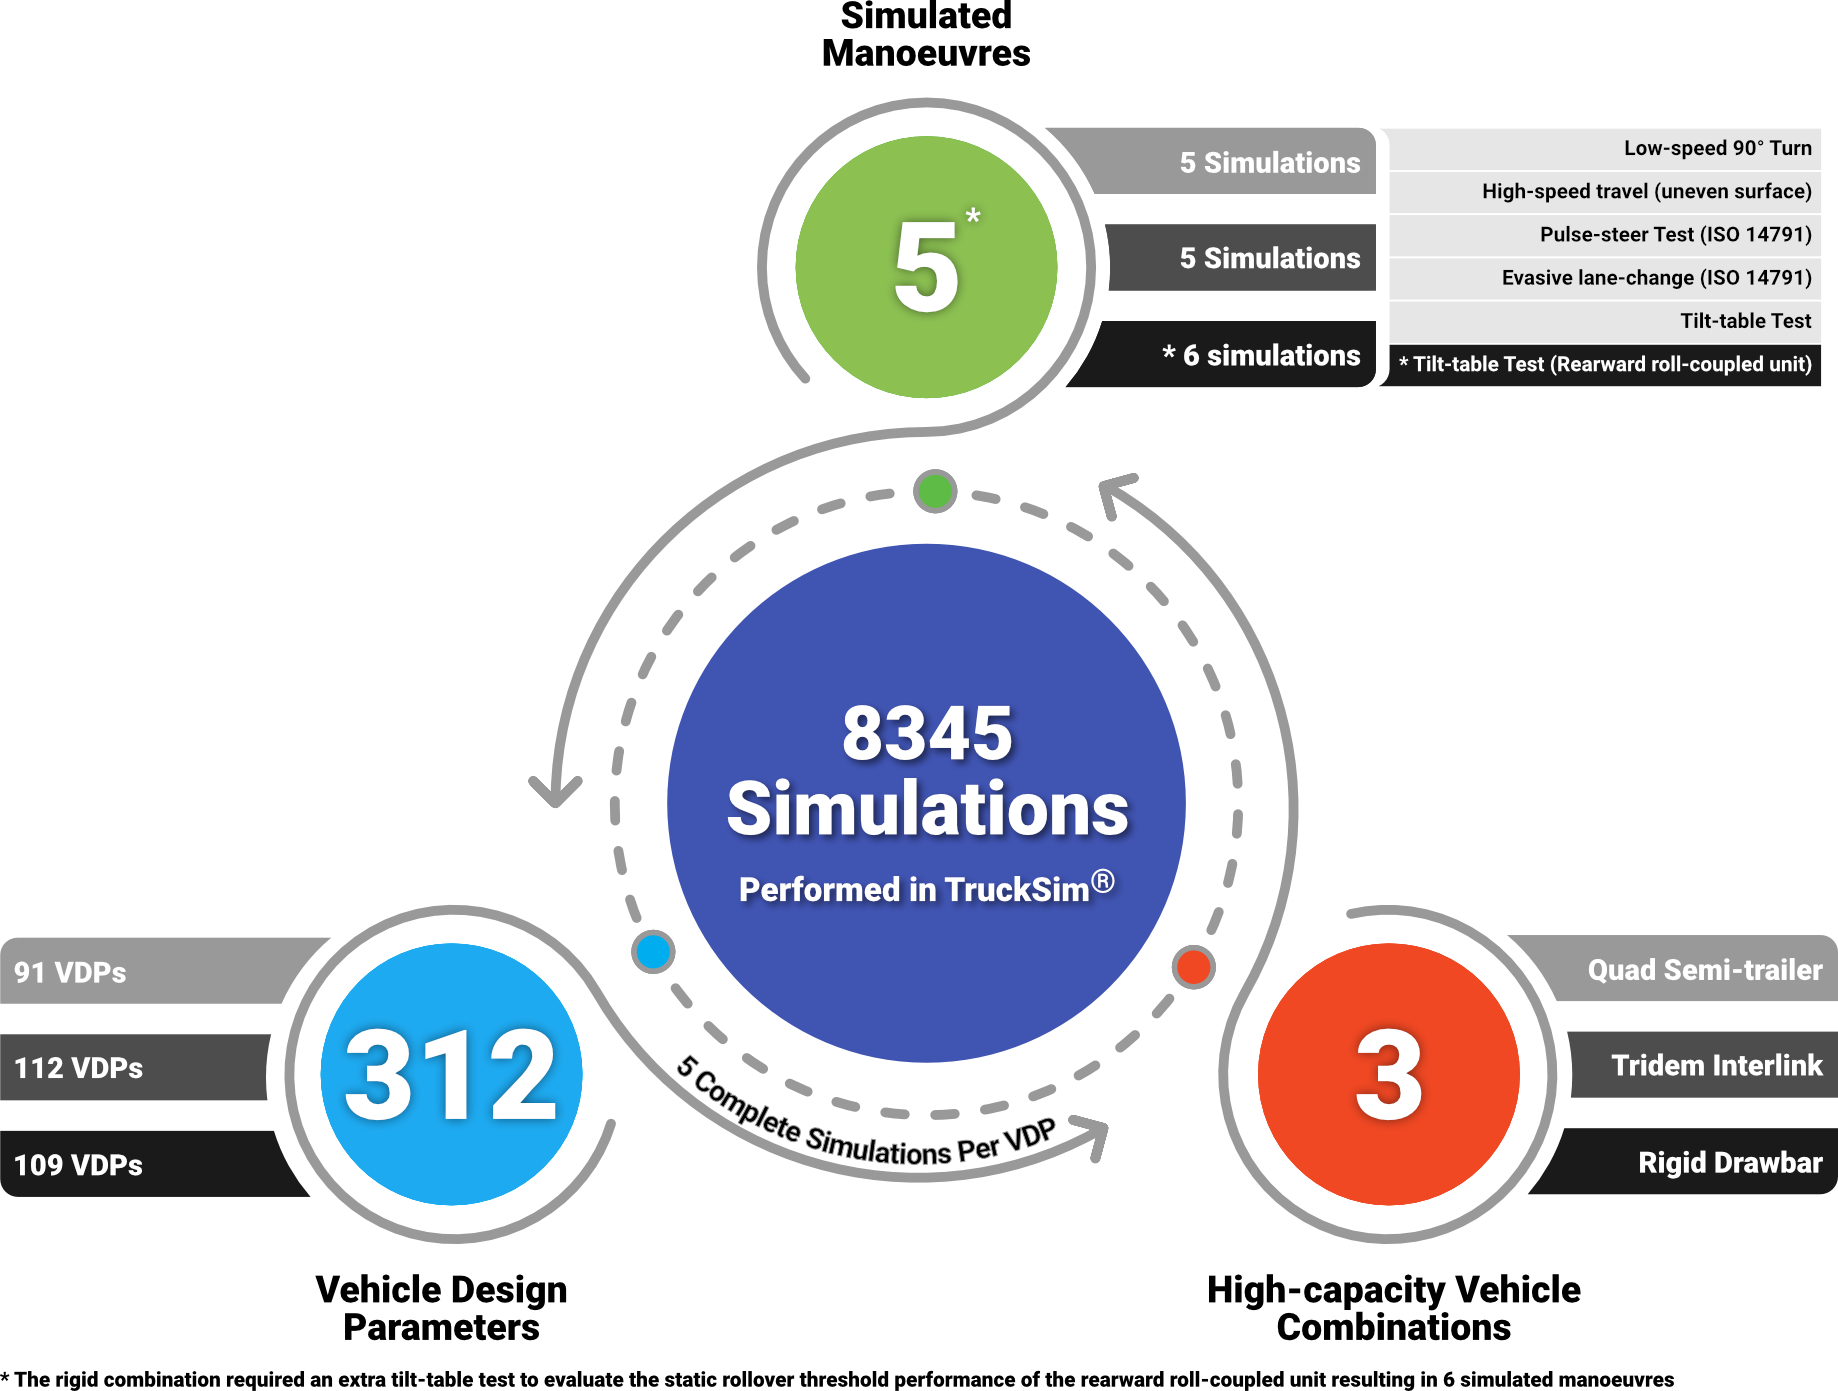
\includegraphics[width=1\textwidth]{fig/Number-of-simulations-Infographic}
	\caption{Overview of the number of \gls{hcv} simulations performed}
	\label{figure:number-of-simulations-overview}
\end{figure}
%----------------------------------------------
%      FIGURE
%----------------------------------------------

\trucksim{} was used as the multi-body vehicle dynamics simulation package to simulate the \gls{hcv} performing a set of \gls{pbs} manoeuvres. The simulation results were used to determine the safety of each \gls{hcv} within the \gls{pbs} framework using a post processor developed in \matlab{} at \gls{wits}. A \matlab{} script automated the adjustment of each individual or combination of parameters within a \trucksim{} model according to the work flow illustrated in Figure~\ref{figure:matlab-trucksim-api-interaction} allowing for the simulation of a large set of vehicle configurations. The versions of each software packaged used are included in Section~\ref{section:software}.

The simulation software and models were calibrated using results published by the \gls{ntc} as detailed in Section~\ref{section:validation-method}.

%----------------------------------------------
%      FIGURE
%----------------------------------------------
\begin{figure}[H]
	\centering
	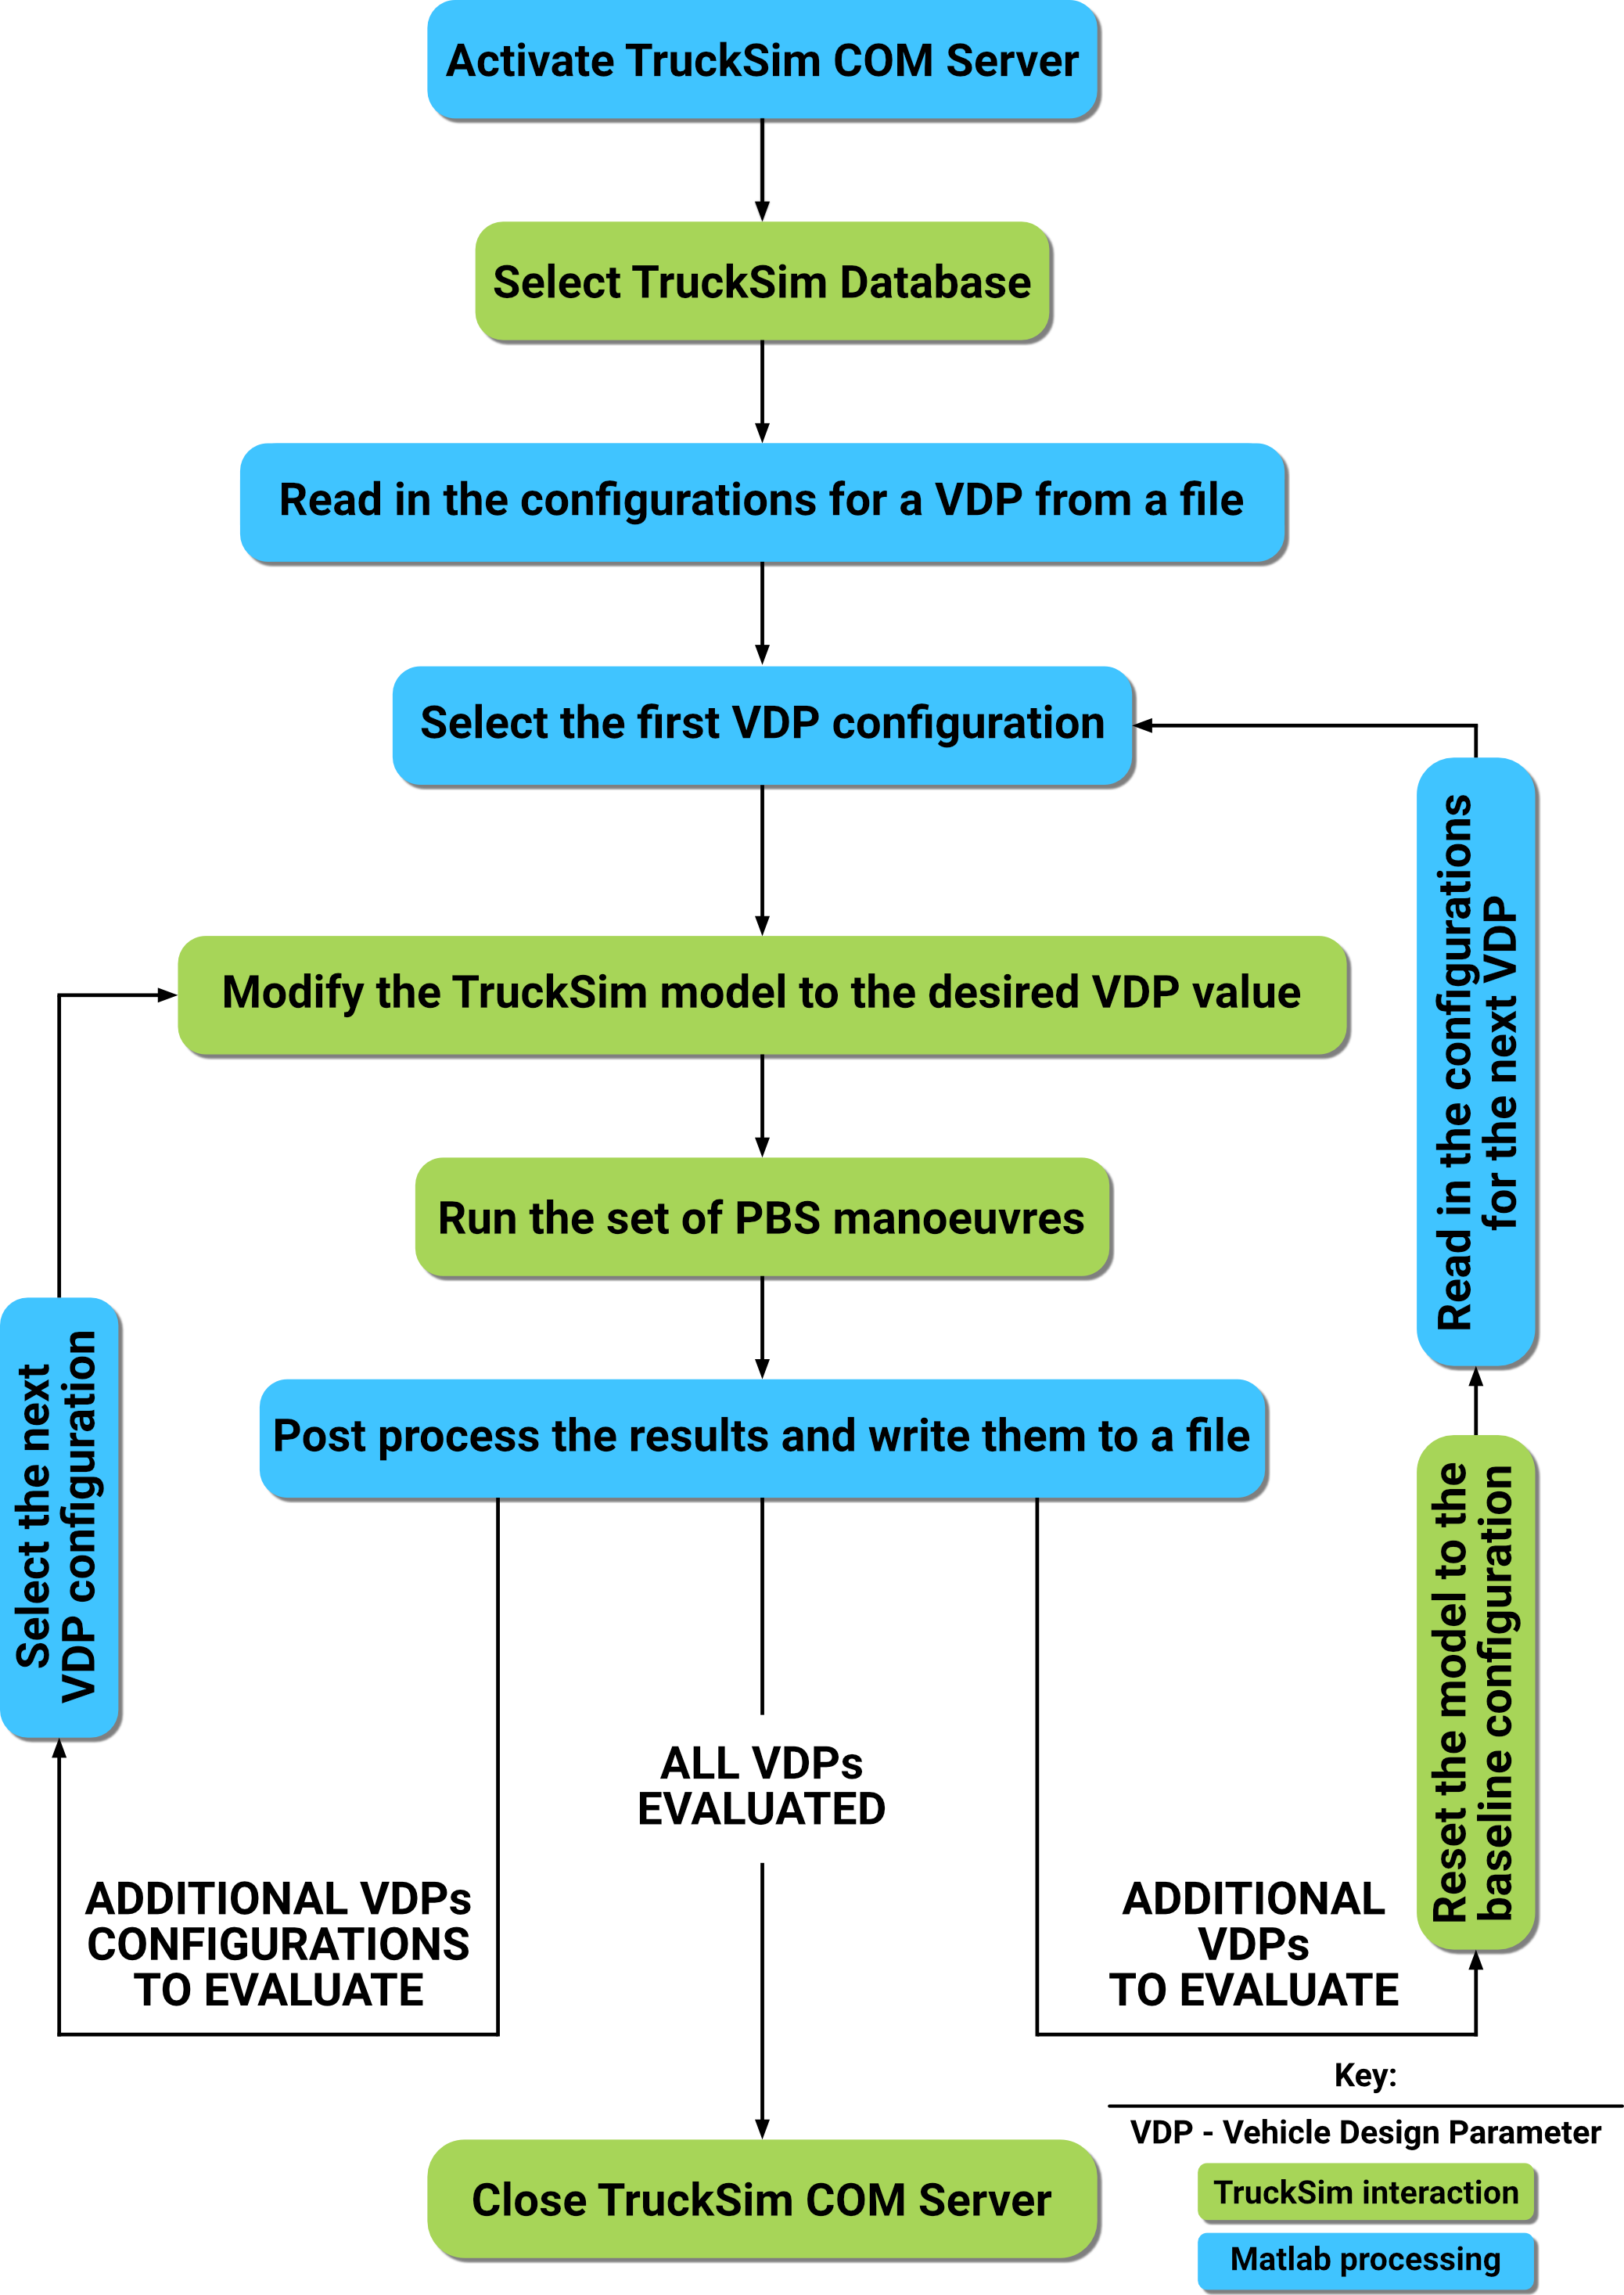
\includegraphics[width=0.75\textwidth]{fig/2018-03-23_trucksim-com-server-flowchart}
	\caption{\matlab{} interaction with the \trucksim{} 2018 API using a COM server}
	\label{figure:matlab-trucksim-api-interaction}
\end{figure}
%----------------------------------------------
%      FIGURE
%----------------------------------------------

%==============================================
%      SECTION
%==============================================
\section{Software}\label{section:software}

The following software packages were used to perform the vehicle simulations:

\begin{enumerate}
	\item \textbf{\trucksim{} 2018 \cite{MechanicalSimulation2016}:} a multi-body vehicle dynamics package used to simulate the various \gls{hcv} vehicle configurations performing the \gls{pbs} manoeuvres.
	\item \textbf{\matlab{} 2018 \cite{MATHWORKS2015}:} a high-level coding environment capable of performing numerical computation and visualisation. Matlab was used in two ways; to post process the simulation outputs of the \trucksim{} simulations and determine vehicle performance within the \gls{pbs} framework and to compare the relative effect of each \gls{vdp} on vehicle performance.
\end{enumerate}

%==============================================
%      SECTION
%==============================================
\section{Software Calibration}\label{section:validation-method}

To perform real world testing to validate the software used to evaluate the \gls{pbs} performance of \glspl{hcv}, experts in the industry were consulted to determine the costs that would be involved. 

In the cost analysis, KDG logistics was consulted to get a quotation of the cost to hire a 6 car car-carrier with a driver and Gerotek was contacted to get a quotation for the use of their test track and tilt-table facilities. An estimated minimum time required to perform the physical testing is included in Table~\ref{table:est-min-time-physical-pbs-testing} (taking into account safety precautions, fitting and testing of sensors that would be used to acquire the data required for validation) and the projected costs of physical testing of a single \gls{hcv} is summarised in Table~\ref{table:est-cost-physical-pbs-testing}. 

The author would like to thank KDG Logistics and Gerotek for their time and efforts involved in providing the quotations.

%----------------------------------------------
%      TABLE
%----------------------------------------------
\begin{table}[H]
	\centering\footnotesize
	\begin{threeparttable}

		\begin{tabulary}{\textwidth}{cc}
			\toprule
\textbf{Manoeuvre}                     & \textbf{Estimated Time Required to Test} \\
			\midrule
Low-speed turn                         & 4 hours                          \\
High-speed lane-change                 & 4 hours                          \\
High-speed tracking on a straight path & 4 hours                          \\
Pulse-steer test                       & 4 hours                          \\
Tilt-table                             & 8 hours                          \\
			\bottomrule
		\end{tabulary}

		\caption{Estimation of the minimum time required to perform physical PBS testing}
		\label{table:est-min-time-physical-pbs-testing}

		%\begin{tablenotes}
		%\item[1] %\tnote{1}
		%\end{tablenotes}

	\end{threeparttable}
\end{table}
%----------------------------------------------
%      TABLE
%----------------------------------------------

Additional funding of R 145 704.00 was not available for validating the software used with the physical testing of a \gls{hcv}. \trucksim{} indicates that their software has been validated and correclated to extensive real-world results as measured and observed by a multitude of well-known automotive \glspl{oem} such as Izuzu, Ford and Toyota along with many others \cite{MechanicalSimulation2018}. Thus, considering the objective of this study is to determine the relative influence of pertinent \glspl{vdp} used as input parameters in multi-body vehicle dynamics simulation software, it was deemed suitable to omit real-world testing and validation and instead perform a calibration of the software according to a framework provided for \gls{pbs} assessors to ensure their simulations are providing accurate results of vehicle safety performance.

%----------------------------------------------
%      TABLE
%----------------------------------------------
\begin{table}[H]
	\centering\footnotesize
	\begin{threeparttable}

		\begin{tabulary}{\textwidth}{lccc}
			\toprule
\textbf{Item}          & \textbf{Cost}     & \textbf{Duration}   & \textbf{Total Cost}  \\
			\midrule

KDG Truck (incl. driver) & R 24 000 per day  & 3 days\tnote{1}    & R72 000.00  \\
Payload Cars           & R 1 800 per day\tnote{1}   & 3 days     & R5 400.00   \\
Gerotek Straight track & R 3 019 per hour  & 16 hours & R48 304.00  \\
Tilt-table test        & R 20 000 per test & One test   & R20 000.00  \\
                       &                   & Total      & R145 704.00 \\
			\bottomrule
		\end{tabulary}

		\caption{Estimation of the minimum time required to perform physical PBS testing}
		\label{table:est-cost-physical-pbs-testing}

		\begin{tablenotes}
		\item[1] Assuming 8 hours per day
		\item[2] Assuming 6 rental vehicles at R 300 each (excluding special insurances)
		\item[3] Assuming the tilt-table test can be completed in a single day
		\end{tablenotes}

	\end{threeparttable}
\end{table}
%----------------------------------------------
%      TABLE
%----------------------------------------------

The \gls{ntc} framework was developed by requesting consultants to compare three computer-based modelling packages (ADAMS, AUTOSIM and \glspl{umtri} Yaw/Roll) to evaluate (in isolation of each other) the \gls{pbs} performance of a B-double and truck-trailer heavy vehicle combination \cite{Prem2001} (known as an interlink and rigid drawbar combination in South Africa).

The \gls{ntc} prescribed a set of inputs for a representative B-double and truck-trailer combination used by all consultants. The vehicles were simulated to perform identical pulse steer, step steer, standard SAE lane change and a low-speed 90\degree{} turn manoeuvres.

The B-double was found to have excellent agreement between all three of the modelling packages. The truck-trailer combination is an inherently less stable vehicle and produced larger but still acceptable amounts of variation in results between the modelling packages.

The Yaw/Roll simulation results were provided by the \gls{ntc} for service providers to calibrate their computer-modelling software and techniques. This data was used to validate the models.

\subsection{Software Calibration Results}\label{section:validation-results}

The behaviour of the B-double and truck-trailer simulated in \trucksim{} 2018 was found to have good correlation with the behaviour simulated in \glspl{umtri} yaw/roll program. Similarly to the outcome of the \gls{ntc} validation, the truck-trailer combination compared less favourably than the B-double combination due to it being a less stable configuration.

Differences in simulated behaviour are attributed to improvements to the prediction of heavy vehicle performance with the latest solvers, differences in the driver models and additional degrees of freedom in the \trucksim{} modelling package.

A set of graphs comparing the simulated vehicle behaviour in \trucksim{} 2018 and \glspl{umtri} yaw/roll program are included in Appendix~\ref{appendix:NTC-validation}.
%----------------------------------------------
%      CHAPTER
%----------------------------------------------
\chapter{Development of the Baseline Vehicles}\label{chapter:baseline-vehicles}

Three of the most productive \gls{hcv} configurations were selected as baselines. A report from the compiled by Nordengen for the \gls{oecd} highlighted that the following combinations were the four most common articulated truck configurations in South Africa \cite{Nordengen2008}:

\begin{enumerate}
	\item A 6x4 truck-tractor hauling a 3-axle semi-trailer
	\item A 6x4 truck-tractor hauling two 2-axle semi-trailers connected with fifth-wheel couplings
	\item A 6x4 truck-tractor hauling a 2-axle semi-trailer
	\item A 6x4 truck-tractor hauling a tridem semi-trailer leader and tandem semi-trailer follower connected with fifth-wheel couplings
\end{enumerate}

Illustrations of each of the workhorse combinations are included in Figure \ref{figure:OECD workhorse combinations}.

%----------------------------------------------
%      FIGURE
%----------------------------------------------
\begin{figure*}[ht!]
	\centering
	\begin{subfigure}[t]{0.45\textwidth}
		\centering
		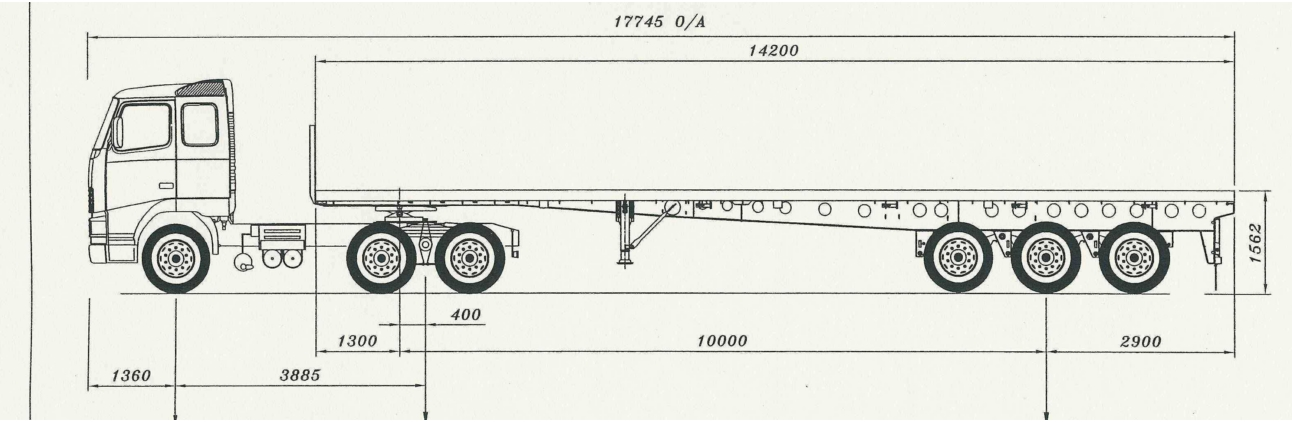
\includegraphics[height=1.0in]{fig/oecd_workhorse-combination_1}
		\caption{Workhorse 1}
	\end{subfigure}%
	\hfill
	\begin{subfigure}[t]{0.45\textwidth}
		\centering
		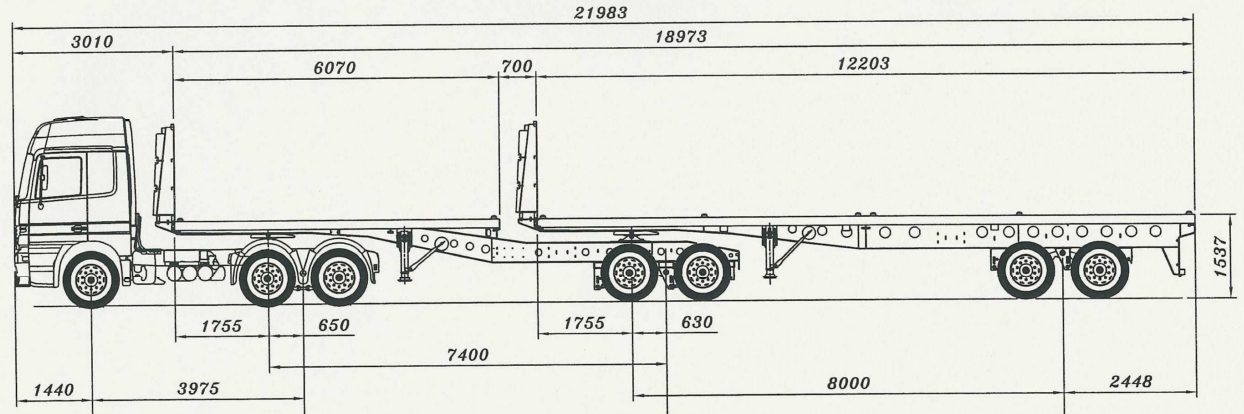
\includegraphics[height=1.0in]{fig/oecd_workhorse-combination_2}
		\caption{Workhorse 2}
	\end{subfigure}

	\begin{subfigure}[t]{0.45\textwidth}
		\centering
		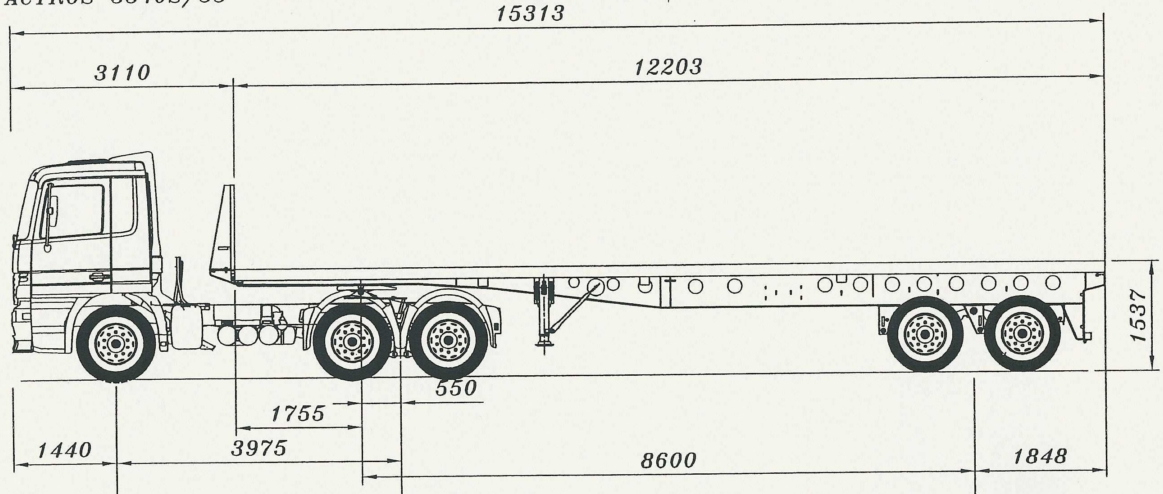
\includegraphics[height=1.0in]{fig/oecd_workhorse-combination_3}
		\caption{Workhorse 3}
	\end{subfigure}
	\hfill
	\begin{subfigure}[t]{0.45\textwidth}
		\centering
		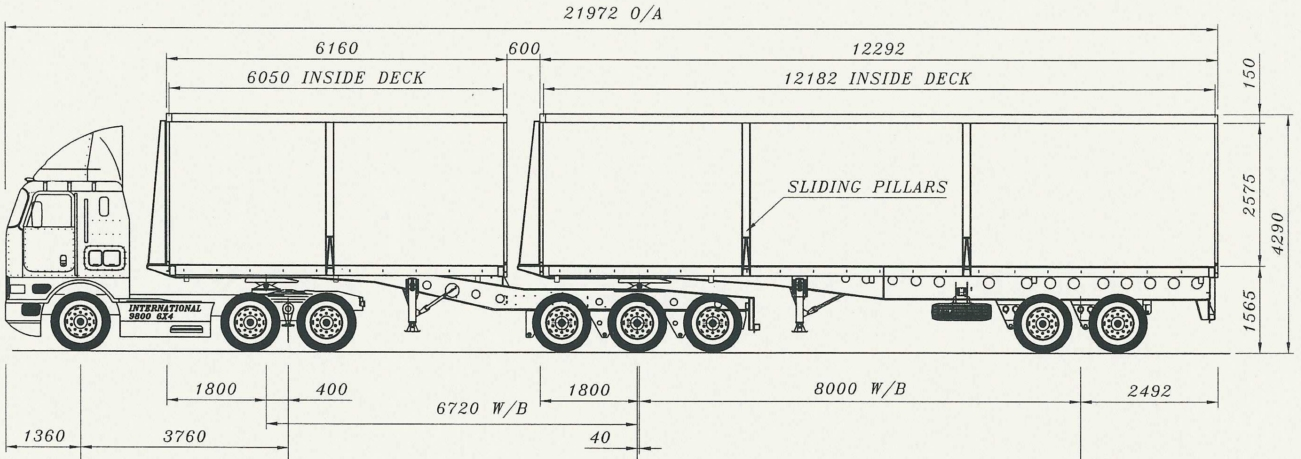
\includegraphics[height=1.0in]{fig/oecd_workhorse-combination_4}
		\caption{Workhorse 4}
	\end{subfigure}
	\caption{OECD workhorse combinations}
	\label{figure:OECD workhorse combinations}
\end{figure*}
%----------------------------------------------
%      FIGURE
%----------------------------------------------

These four workhorse vehicles have during the \gls{pbs} pilot project in South Africa been replaced by two more productive \gls{pbs} equivalents which were chosen as the first two baseline combinations:

\begin{enumerate}
	\item A 6x4 truck-tractor hauling a quad-axle semi-trailer
	\item A 6x4 truck-tractor hauling a set of tridem semi-trailers
\end{enumerate}

As of 2016 a rigid drawbar combination (known as a truck and dog combination in Australia) was still the single biggest category of vehicles approved via \gls{pbs} as can be seen in Figure \ref{figure:distribution-of-australian-pbs-fleet} \cite{Grote2017}. These combinations are not very prevalent in South Africa outside of the forestry industry, however it is envisioned that as the pilot project progresses in South Africa and \gls{pbs} becomes more widely adopted, that this combination will become widely-used.

%----------------------------------------------
%      FIGURE
%----------------------------------------------
\begin{figure}[H]
	\centering
	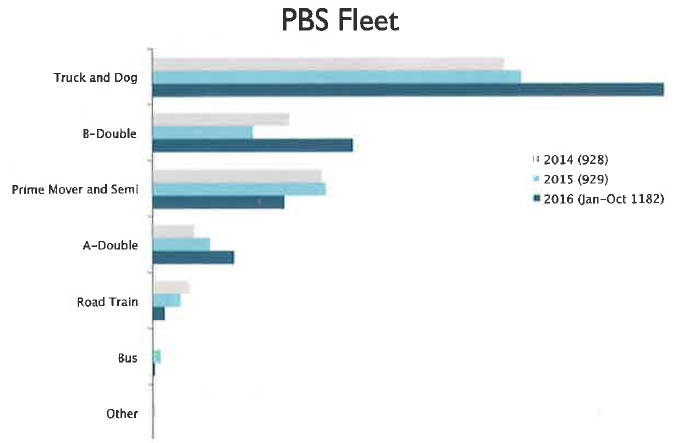
\includegraphics[width=1\textwidth]{fig/globaltrailermag_truck-and-dog-pbs-fleet-australia}
	\caption{Distribution of the Australian PBS fleet as of Oct 2016 \cite{Grote2017}}
	\label{figure:distribution-of-australian-pbs-fleet}
\end{figure}
%----------------------------------------------
%      FIGURE
%----------------------------------------------

%----------------------------------------------
%      SECTION
%----------------------------------------------
\section{Design Parameters for the Baseline Vehicles}\label{section:baseline-vehicles-design-parameters}

The design of the mechanical properties of the baseline vehicles is beyond the scope of this dissertation. Thus, combinations matching the designs chosen for baseline vehicles that were assessed within the \gls{pbs} framework in South Africa were used as a guide to develop the baseline combinations.

The baseline combinations use the same baseline prime mover (for which data was provided by the \gls{oem}) with the geometrical properties of the prime mover (such as the wheelbase and hitch location) modified to suit the design of each baseline combination.

Representative axles were developed for the baseline combinations. The prime movers used the same set of steer and drive axles and the trailer axles differed in track width and tyre size for each trailer.

Sections~\ref{section:baseline-quad-semi}~to~\ref{section:baseline-rigid-drawbar-combination} describe the configuration of each baseline combination according to the baseline prime mover units, trailer units and axles.

%      SUBSECTION
%----------------------------------------------
\subsection{Baseline Quad Semi-trailer Combination}\label{section:baseline-quad-semi}

The quad semi-trailer fuel tanker is one of the most common quad-axle semi-trailer combinations operated in South Africa. A \gls{lpg} quad was selected as the baseline for this combination. The configuration of this baseline combination is as per Table~\ref{table:configuration-quad-semi} and a simplified \gls{ga} drawing of the combination is included in Figure \ref{figure:baseline-ga-quad-semi}.

%----------------------------------------------
%      TABLE
%----------------------------------------------
\begin{table}[H]
	\centering\footnotesize
	\begin{threeparttable}

		\begin{tabulary}{\textwidth}{llc}
			\toprule
\textbf{Vehicle unit, axle or tyre} & \textbf{Description} & \textbf{VDP Table (see Appendix~\ref{appendix:baseline-models})} \\
		\midrule
    Prime mover unit & Truck tractor & Table~\ref{table:vdp-range-prime-mover-tractor} \\
    Trailer unit & Quad semi-trailer & Table~\ref{table:vdp-range-trailer-quad-semi} \\
    Steer axle  & Steer axle with 315/80 R22.5 tyres & Table~\ref{table:vdp-range-axle-steer-315} \\
    Drive axle & Drive axle with 315/80 R22.5 tyres & Table~\ref{table:vdp-range-axle-drive-315} \\
    Trailer axle & Trailer axle with 445/65 R22.5 tyres & Table~\ref{table:vdp-range-axle-trailer-445} \\
    Steer tyre & 315/80 R22.5 (singles) & Table~\ref{table:vdp-tyre-315} \\
    Drive tyre  & 315/80 R22.5 (duals) & Table~\ref{table:vdp-tyre-315} \\
    Trailer tyre & 445/65 R22.5 (singles) & Table~\ref{table:vdp-tyre-445} \\
			\bottomrule
		\end{tabulary}

		\caption{Configuration of the baseline quad-semi combination}
		\label{table:configuration-quad-semi}

		%\begin{tablenotes}
		%\item[1] %\tnote{1}
		%\end{tablenotes}

	\end{threeparttable}
\end{table}
%----------------------------------------------
%      TABLE
%----------------------------------------------

\newpage

\newgeometry{left=5mm,right=5mm,top=5mm,bottom=10mm, footskip=0mm}

\begin{landscape}\centering
\vspace*{\fill}
%----------------------------------------------
%      FIGURE
%----------------------------------------------
\begin{figure}[H]
	\centering
	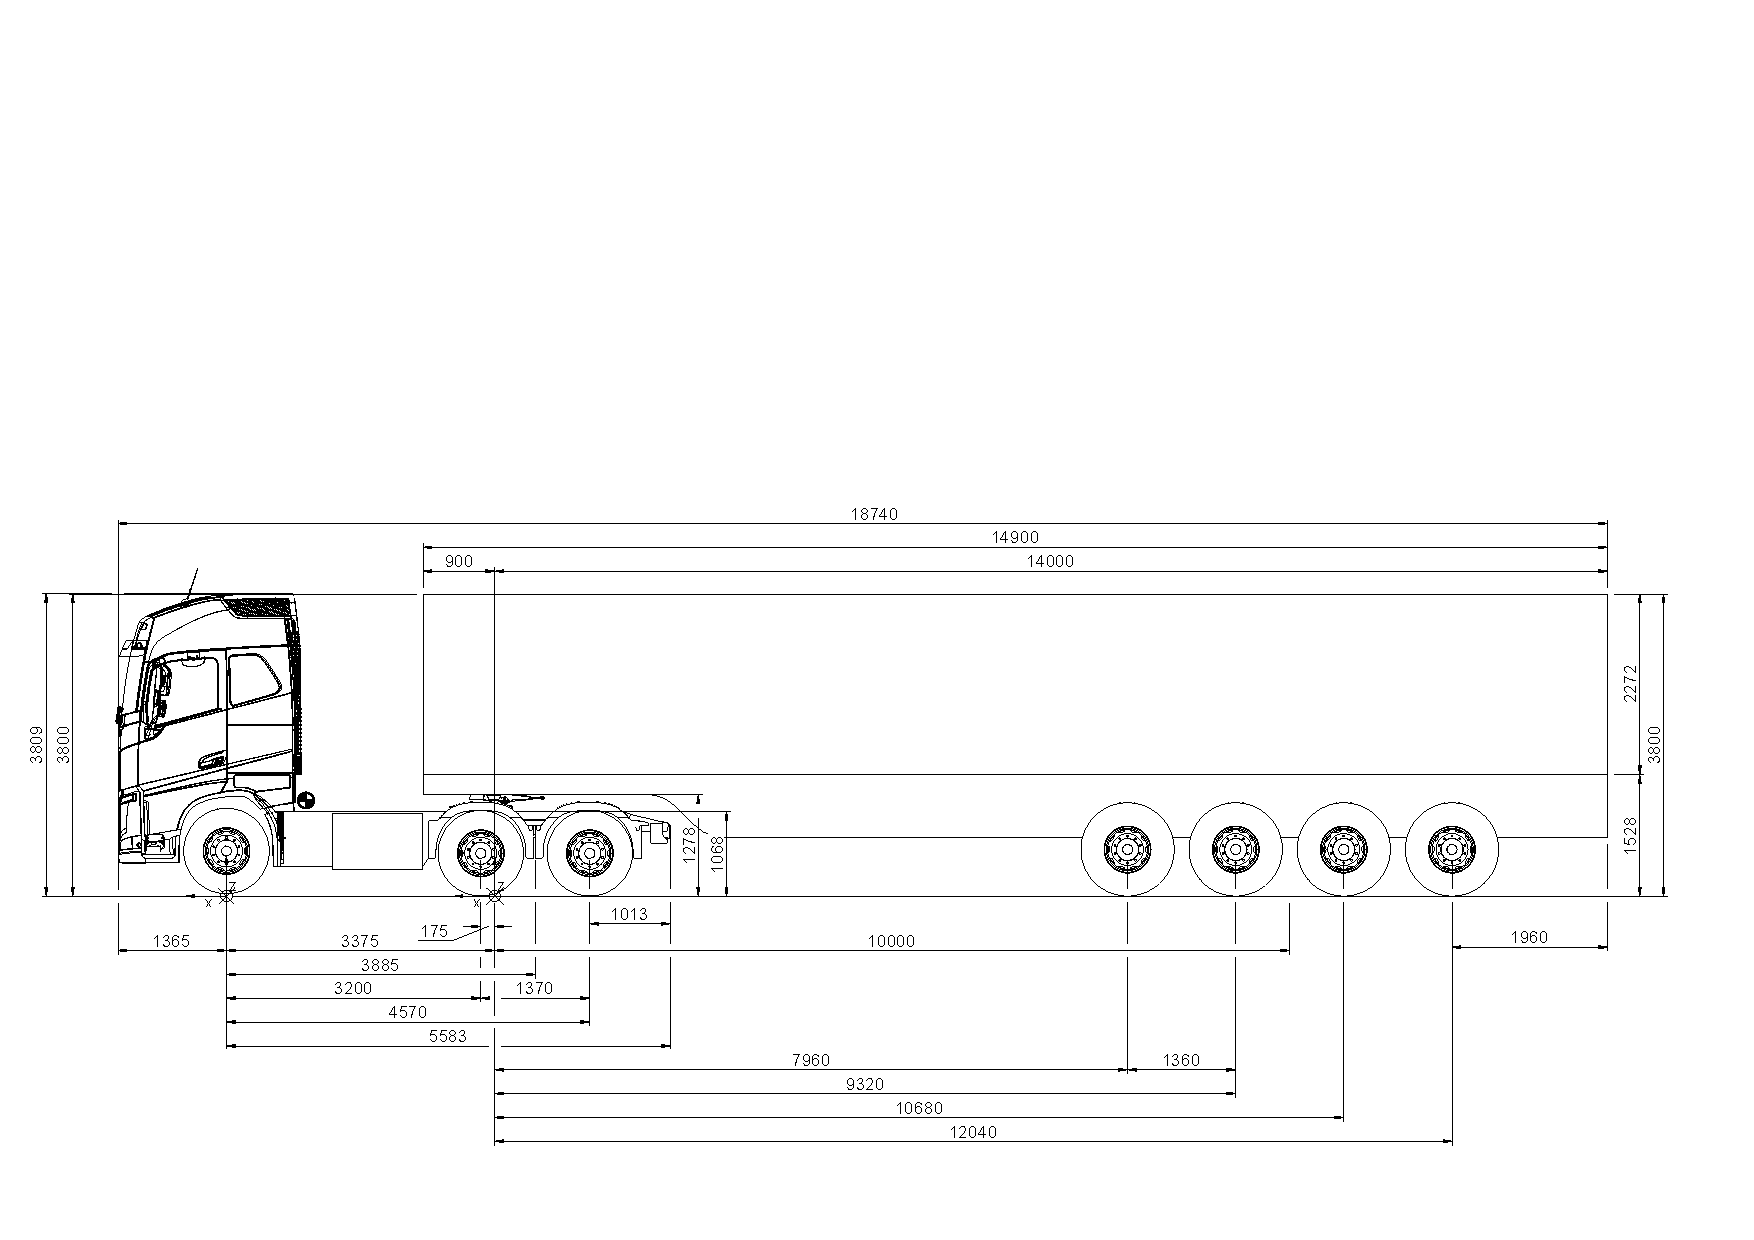
\includegraphics[width=1.3\textwidth]{fig/baseline_ga_quad-semi}
	\caption{Baseline quad semi-trailer combination GA drawing}
	\label{figure:baseline-ga-quad-semi}
\end{figure}
%----------------------------------------------
%      FIGURE
%----------------------------------------------
\vfill
\end{landscape}

\restoregeometry



%      SUBSECTION
%----------------------------------------------
\subsection{Baseline Tridem Interlink Combination}\label{section:baseline-tridem-interlink}

A tridem interlink side-tipper used for the transportation of coal ore was modelled as the baseline tridem interlink combination. The configuration of this baseline combination is as per Table~\ref{table:configuration-tridem-interlink} and a \gls{ga} drawing of the combination is included in Figure~\ref{figure:baseline-ga-tridem-interlink}.

%----------------------------------------------
%      TABLE
%----------------------------------------------
\begin{table}[H]
	\centering\footnotesize
	\begin{threeparttable}

		\begin{tabulary}{\textwidth}{llc}
			\toprule
    \textbf{Vehicle unit, axle or tyre} & \textbf{Description} & \textbf{VDP Table (see Appendix~\ref{appendix:baseline-models})} \\
    			\midrule
    Prime mover unit & Truck tractor & Table~\ref{table:vdp-range-prime-mover-tractor} \\
    Lead trailer unit & Tridem interlink leader & Table~\ref{table:vdp-range-trailer-tridem-interlink-leader} \\
    Follower trailer unit & Tridem interlink follower & Table~\ref{table:vdp-range-trailer-tridem-interlink-follower} \\
    Steer axle  & Steer axle with 315/80 R22.5 tyres & Table~\ref{table:vdp-range-axle-steer-315} \\
    Drive axle & Drive axle with 315/80 R22.5 tyres & Table~\ref{table:vdp-range-axle-drive-315} \\
    Trailer axle & Trailer axle with 315/80 R22.5 tyres & Table~\ref{table:vdp-range-axle-trailer-315} \\
    Steer tyre & 315/80 R22.5 (singles) & Table~\ref{table:vdp-tyre-315} \\
    Drive tyre  & 315/80 R22.5 (duals) & Table~\ref{table:vdp-tyre-315} \\
    Trailer tyre & 315/80 R22.5 (duals) & Table~\ref{table:vdp-tyre-315} \\
			\bottomrule
		\end{tabulary}

		\caption{Configuration of the baseline tridem interlink combination}
		\label{table:configuration-tridem-interlink}

		%\begin{tablenotes}
		%\item[1] %\tnote{1}
		%\end{tablenotes}

	\end{threeparttable}
\end{table}
%----------------------------------------------
%      TABLE
%----------------------------------------------

\newgeometry{left=5mm,right=5mm,top=5mm,bottom=10mm, footskip=0mm}

\begin{landscape}\centering
	\vspace*{\fill}
%----------------------------------------------
%      FIGURE
%----------------------------------------------
\begin{figure}[H]
	\centering
	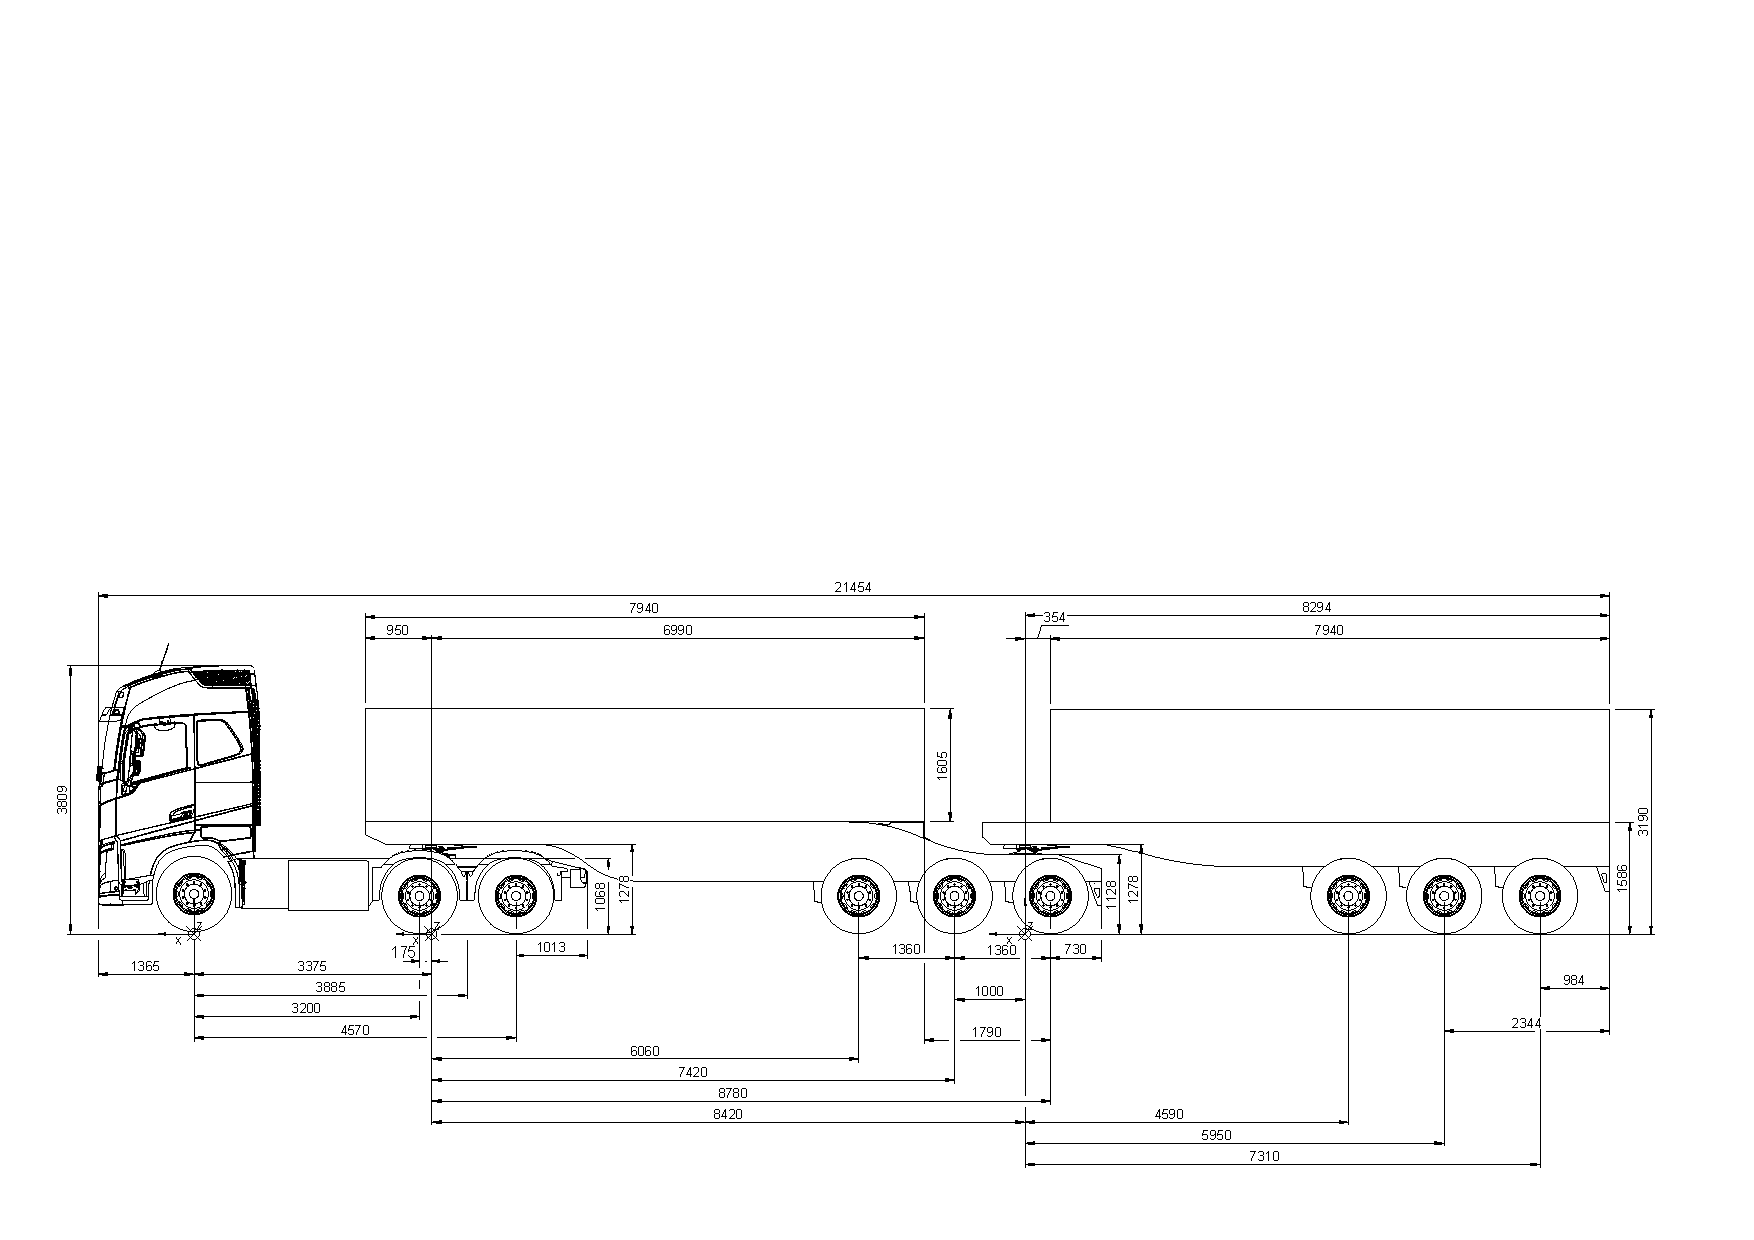
\includegraphics[width=1.3\textwidth]{fig/baseline_ga_tridem-interlink}
	\caption{Baseline tridem interlink combination GA drawing}
	\label{figure:baseline-ga-tridem-interlink}
\end{figure}
%----------------------------------------------
%      FIGURE
%----------------------------------------------
	\vfill
\end{landscape}

\restoregeometry

%      SUBSECTION
%----------------------------------------------
\subsection{Baseline Rigid Drawbar Combination}\label{section:baseline-rigid-drawbar-combination}

The rigid drawbar combination is most prevalent in South Africa in the logging industry. The baseline rigid drawbar combination was modelled from a combination intended for the transport of timber. The configuration of this baseline combination is as per Table~\ref{table:configuration-rigid-drawbar-combination} and a simplified \gls{ga} drawing of the combination is included in Figure~\ref{figure:baseline-ga-rigid-drawbar-combination}.

%----------------------------------------------
%      TABLE
%----------------------------------------------
\begin{table}[H]
	\centering\footnotesize
	\begin{threeparttable}

		\begin{tabulary}{\textwidth}{llc}
			\toprule
    \textbf{Vehicle unit, axle or tyre} & \textbf{Description} & \textbf{VDP Table (see Appendix~\ref{appendix:baseline-models})} \\
    			\midrule
    Prime mover unit & Rigid truck & Table~\ref{table:vdp-range-prime-mover-rigid} \\
    Lead trailer unit & Tridem semi-trailer & Table~\ref{table:vdp-range-trailer-rigid-combination-trailer} \\
    Dolly unit & Dolly & Table~\ref{table:vdp-range-trailer-rigid-combination-dolly} \\
    Steer axle  & Steer axle with 315/80 R22.5 tyres & Table~\ref{table:vdp-range-axle-steer-315} \\
    Drive axle & Drive axle with 315/80 R22.5 tyres & Table~\ref{table:vdp-range-axle-drive-315} \\
    Trailer axle\tnote{1} & Trailer axle with 285/70 R19.5 tyres & Table~\ref{table:vdp-range-axle-trailer-285} \\
    Steer tyre & 315/80 R22.5 (singles) & Table~\ref{table:vdp-tyre-315} \\
    Drive tyre  & 315/80 R22.5 (duals) & Table~\ref{table:vdp-tyre-315} \\
    Trailer tyre\tnote{1} & 285/70 R19.5 (duals) & Table~\ref{table:vdp-tyre-285} \\
			\bottomrule
		\end{tabulary}

		\caption{Configuration of the baseline rigid drawbar combination}
		\label{table:configuration-rigid-drawbar-combination}

		\begin{tablenotes}
		\item[1] The dolly axle is considered as a trailer axle
		\end{tablenotes}

	\end{threeparttable}
\end{table}
%----------------------------------------------
%      TABLE
%----------------------------------------------

\newgeometry{left=5mm,right=5mm,top=5mm,bottom=10mm, footskip=0mm}

\begin{landscape}\centering
	\vspace*{\fill}
%----------------------------------------------
%      FIGURE
%----------------------------------------------
\begin{figure}[H]
	\centering
	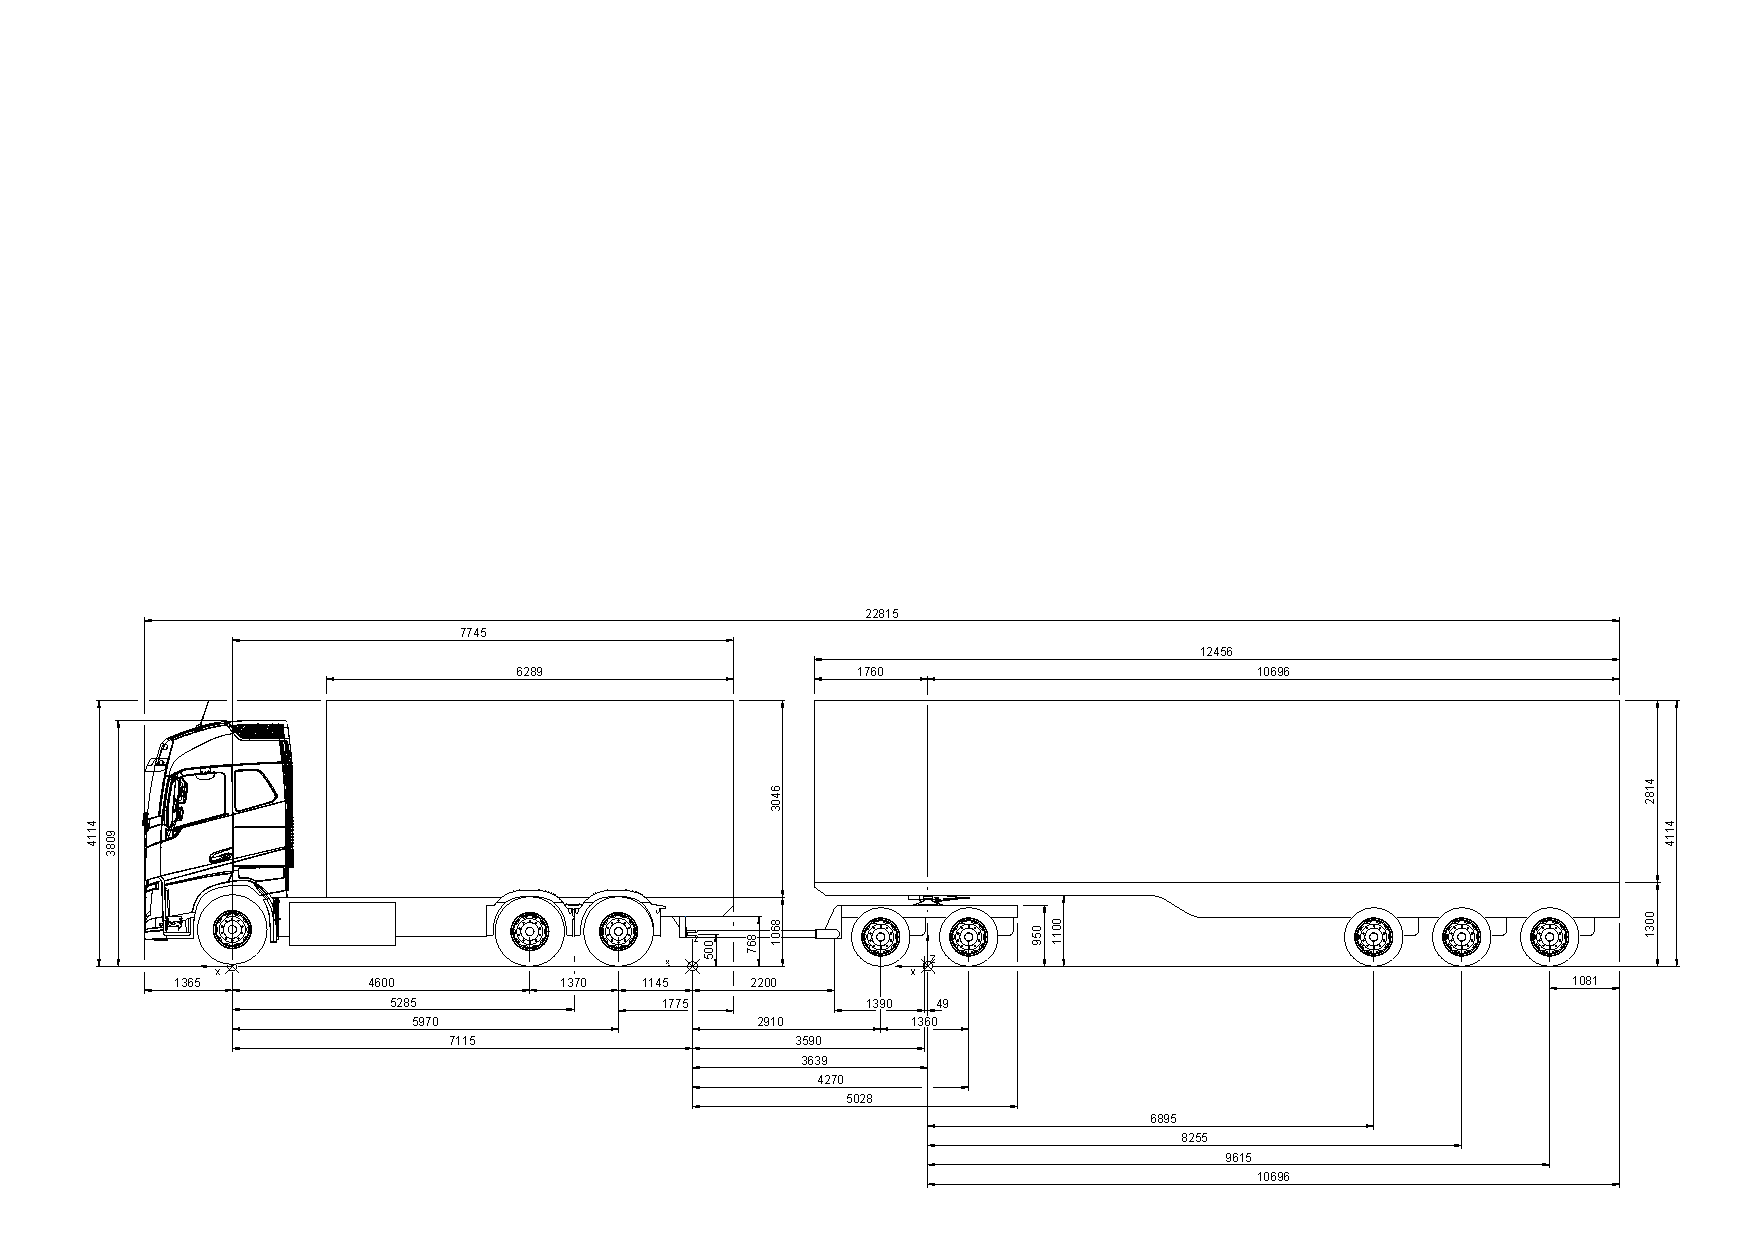
\includegraphics[width=1.3\textwidth]{fig/baseline_ga_rigid-drawbar}
	\caption{Baseline rigid drawbar combination GA drawing}
	\label{figure:baseline-ga-rigid-drawbar-combination}
\end{figure}
%----------------------------------------------
%      FIGURE
%----------------------------------------------
	\vfill
\end{landscape}

\restoregeometry
\chapter{VDP Range Selection}\label{chapter:parameter-range-selection}

Ensuring that the ranges for each \gls{vdp} are realistic and representative is critical in accurately quantifying the relative influence of each \gls{vdp}. Overestimating a \gls{vdp} range will overestimate its relative influence and vica versa underestimating a \gls{vdp} range would underestimate its relative influence. The rationale for selecting the ranges for each \gls{vdp} is presented in the sections that follow.

%==============================================
%      SECTION
%==============================================
\section{Geometric Parameter Limits}\label{section:geometric-limits}

The \gls{pbs} scheme is still in the pilot project stages in South Africa and as part of the pilot project the vehicles that form part of the \gls{pbs} fleet still need to adhere to certain regulations as stipulated within the \gls{nrta} unless special permission is given by the \gls{ndot} in the form of a operational approval.

The \gls{pbs} scheme is designed to develop safer, more productive \glspl{hcv} without the requirement of being governed by a prescriptive framework. Kienh{\"o}fer et al. \cite{Kienhofer2014} evaluated the \gls{mod} and \gls{dom} performance and highlighted that the prescriptive framework allows for the most lenient geometrical constraints for frontal overhang when compared to Australia, the European Union, Canada, and the United States. Thus, the prescriptive framework was used as a guide to determine the maximum dimensional limits for each combination while simultaneously ensuring that the geometry would be structurally possible with the baseline design. The prescriptive legislation for maximum vehicle dimensions in South Africa is detailed in Part III of the \gls{nrta} (Act No. 93 of 1996) \cite{NationalDepartmentofTransport2003} and any regulation numbers included in the tables below refer to this document.

The vehicle geometry plays the largest role in the low-speed performance (\gls{lssp}, \gls{fs}, \gls{ts}, \gls{mod}, \gls{dom}). The geometrical reference points used to calculate these are described in the \gls{pbs} scheme \cite{NationalTransportCommission2008} as follows:

\begin{enumerate}
	\item \textbf{Forward reference points:} \enquote{the vertical projection of the furthest forward or outside point, or points, on the vehicle}
	\item \textbf{Rear reference points:} \enquote{the vertical projection of the furthest rearward or outside point, or points, on the vehicle}
\end{enumerate}

Minimum dimensional limits are not explicitly defined in the \gls{nrta} and have been determined according to either physical constraints or other limitations which will be discussed in the sections that follow.

%      SUBSECTION
%----------------------------------------------
\subsection{Front Overhang}\label{section:pr-frontal-overhang}

A representative frontal overhang for the prime movers was determined from \gls{oem} catalogues, the data from which is included in Table~\ref{table:oem-front-overhang}.

%----------------------------------------------
%      TABLE
%----------------------------------------------
\begin{table}[H]
	\centering\footnotesize
	\begin{threeparttable}

		\begin{tabulary}{\textwidth}{lc}
			\toprule
			\textbf{Prime mover model} & \textbf{Front overhang (mm)} \\
			\midrule
			Volvo FH42T3LA \cite{VolvoTruckCorporation2017FH42T3LA} & 1365 \\
			Mercedes Benz Atego \cite{MercedesBenzAtego2015} & 1380 \\
			Scania G440/480 8x4 \cite{ScaniaG4404806x4} & 1455 \\
			DAF FTT XF105.460 \cite{DAFXF105.4602017} & 1370 \\
			Volvo FM64T3HBX \cite{VolvoTruckCorporation2018FM64T3HBX} & 1520 \\
			\bottomrule
		\end{tabulary}

		\caption{OEM prime mover front overhangs\tnote{1}}
		\label{table:oem-front-overhang}

		\begin{tablenotes}
			\item[1] SAE up co-ordinate system and origin taken from centre of steer axle or hitch point (for trailers) at ground level
		\end{tablenotes}

	\end{threeparttable}
\end{table}
%----------------------------------------------
%      TABLE
%----------------------------------------------

Regulation 221 in the \gls{nrta} allows for a 300 mm projection forward of the front of cab for a bull-bar and therefore considering a worst case frontal cab overhang of 1520~mm, the maximum overhang with a bull-bar will be considered 300~mm ahead of this at the same width of the cab.

The front overhang in the case of the trailer units and rigid truck were limited according to regulation 226 (1)(a) which allows a frontal overhang of up to 1800~mm for a semi-trailer.  The swing radius of all the models were checked to ensure that there would be no collision with the unit ahead of it. The limit was set such that there would be a 50 mm clearance between the leading unit and the swing radius of the following unit.

In the case of the tridem interlink follower, the baseline frontal overhang is negative (behind the hitch) which was used as the minimum. All other trailer frontal overhangs were evaluated as 0~mm from the hitch connection assuming a narrow chassis section extends further to structurally support the 5th wheel hitch connection.

The resulting parameter range for the front overhangs of each unit is provided in Table~\ref{table:parameter-range-front-overhang}.

%----------------------------------------------
%      TABLE - UPDATED TO NEW RANGES
%----------------------------------------------
\begin{table}[H]
	\centering\footnotesize
	\begin{threeparttable}

		\begin{tabulary}{\textwidth}{lcccll}
			\toprule
			\textbf{Vehicle unit} & \textbf{Baseline (mm)} & \textbf{Min. (mm)} & \textbf{Max. (mm)} & \textbf{Rationale min.} & \textbf{Rationale max.} \\
			\midrule
            Truck tractor & 1365  & 1300  & 1820  & OEM variations & OEM variations \\
            Rigid truck & 1365  & 1300  & 1820  & OEM variations & OEM variations \\
            Quad semi-trailer & 900   & 0     & 1800  & Structural & Regulation 226 (a) \\
            Tridem interlink leader & 950   & 0     & 1800  & Structural & Regulation 226 (a) \\
            Tridem interlink follower & -354  & -354  & 464   & Structural & Structural \\
            Tridem semi-trailer & 1760  & 0     & 1800  & Structural & Regulation 226 (a) \\
			\bottomrule
		\end{tabulary}

		\caption{Parameter range - front overhang\tnote{1}}
		\label{table:parameter-range-front-overhang}

		\begin{tablenotes}
			\item[1] SAE up co-ordinate system and origin taken from centre of steer axle or hitch point (for trailers) at ground level
		\end{tablenotes}

	\end{threeparttable}
\end{table}
%----------------------------------------------
%      TABLE
%----------------------------------------------

%      SUBSECTION
%----------------------------------------------
\subsection{Rear Overhang}\label{section:pr-rear-overhang}

All rear overhangs were considered at the point where the structure of the unit was at its widest. Narrow chassis extensions were ignored.

Regulation 226 (2)(c) states that the maximum rear overhang of any semi-trailer or other vehicle (other than refuse collectors, road making, road construction, farming  vehicles and vehicles with a single axle or axle unit) may not exceed 60 \% of the wheelbase measured from the centre of the rearmost axle on the unit. This was considered along with structural constraints to develop the maximum rear overhang reference points.

The reference point evaluated for the rear overhang of the 6x4 truck-tractor is at the furthest rear and widest point on the wheel arch. Further past this, the chassis extension is narrow and is not used as a reference point in the manoeuvres. As a result, the rear overhang was not evaluated for this vehicle unit.

In the case of the rigid truck, the superstructure could legally extend further back to the NRTA limit of 60\% of the wheelbase. This would cause the rigid payload to extend into the rear semi-trailer. Considering the swing radius of the rear trailer of 2188 mm, the maximum rear overhang of the rigid payload with a 50 mm clearance to ensure no contact in dynamic manoeuvres would be 2546 mm from the rear axle as can be seen in Figure~\ref{figure:parameter-selection-rear-overhang-of-rigid-truck}

%----------------------------------------------
%      FIGURE
%----------------------------------------------
\begin{figure}[H]
	\centering
	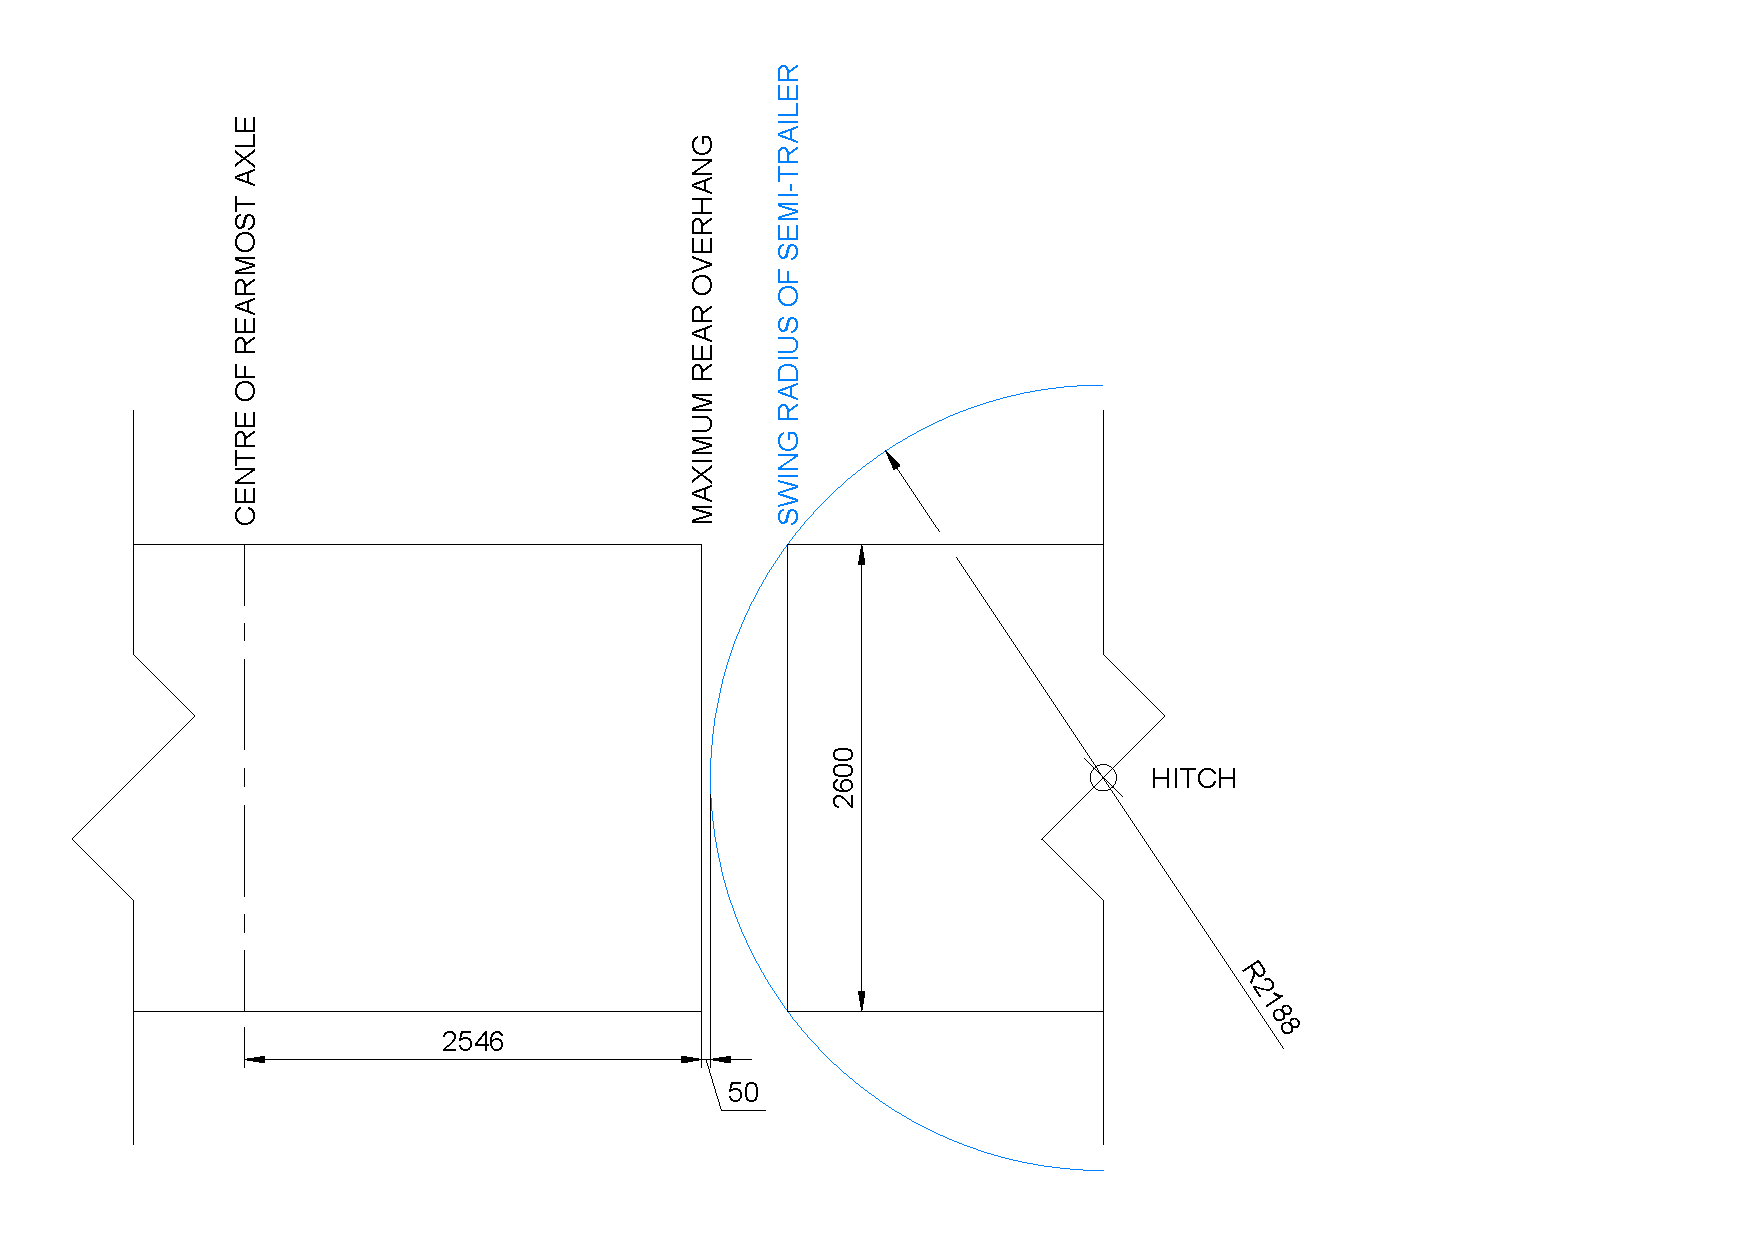
\includegraphics[width=1\textwidth]{fig/parameter-selection_rear-overhang_rigid-truck}
	\caption{Rear overhang of the rigid truck}
	\label{figure:parameter-selection-rear-overhang-of-rigid-truck}
\end{figure}
%----------------------------------------------
%      FIGURE
%----------------------------------------------

Similarly, the maximum rear overhang for the tridem interlink leader was determined geometrically from the swing radius of the narrow follower chassis as shown in Figure~\ref{figure:parameter-selection-rear-overhang-of-b-double-leader}.

%----------------------------------------------
%      FIGURE
%----------------------------------------------
\begin{figure}[H]
	\centering
	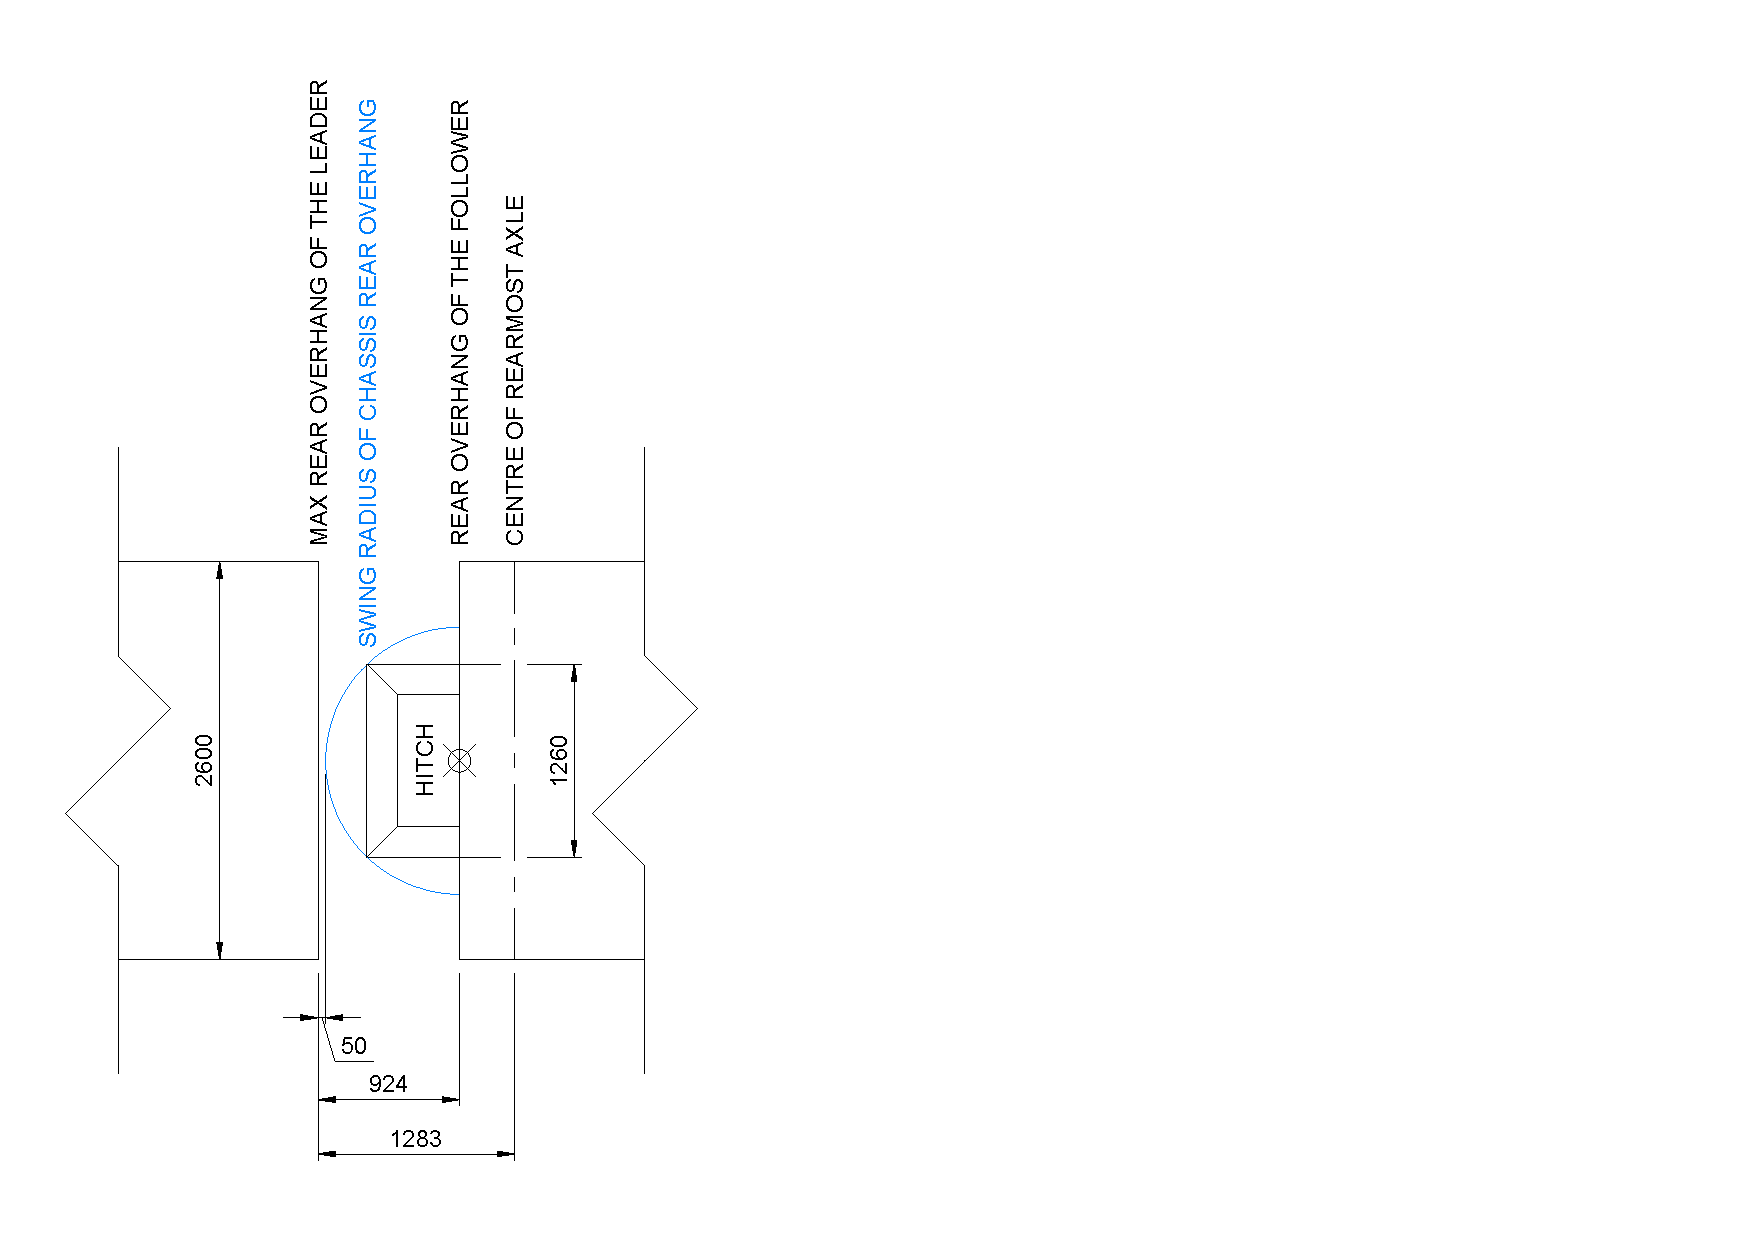
\includegraphics[width=0.7\textwidth]{fig/parameter-selection_rear-overhang_b-double-leader}
	\caption{Rear overhang of the tridem interlink leader trailer}
	\label{figure:parameter-selection-rear-overhang-of-b-double-leader}
\end{figure}
%----------------------------------------------
%      FIGURE
%----------------------------------------------

The resulting range of rear overhangs is summarised in Table~\ref{table:parameter-range-rear-overhang}.

%----------------------------------------------
%      TABLE - UPDATED TO NEW RANGES
%----------------------------------------------
\begin{table}[H]
	\centering\footnotesize
	\begin{threeparttable}

		\begin{tabulary}{\textwidth}{lcccll}
			\toprule
			\textbf{Vehicle unit} & \textbf{Baseline (mm)} & \textbf{Min. (mm)} & \textbf{Max. (mm)} & \textbf{Rationale min.} & \textbf{Rationale max.} \\
			\midrule
            Truck tractor & 1013  & 1013  & 1013  & No impact & No impact \\
            Rigid truck & 1775  & 0     & 2546  & Assumption & Structural \\
            Quad semi-trailer & 1960  & 0     & 6000  & Assumption & Regulation 226 (2)(c) \\
            Tridem interlink leader & -1790 & -1790 & -1283 & Structural & Structural \\
            Tridem interlink follower & 984   & 0     & 3570  & Assumption & Structural \\
            Tridem semi-trailer & 1081  & 0     & 4953  & Assumption & Regulation 226 (2)(c) \\
			\bottomrule
		\end{tabulary}

		\caption{Parameter range - rear overhang \tnote{1}}
		\label{table:parameter-range-rear-overhang}

		\begin{tablenotes}
			\item[1] Measured from the centre of the rearmost axle in accordance with Regulation 226 (2)(c)
		\end{tablenotes}

	\end{threeparttable}
\end{table}
%----------------------------------------------
%      TABLE
%----------------------------------------------

%      SUBSECTION
%----------------------------------------------
\subsection{Vehicle Width}\label{section:pr-vehicle-width}

The maximum width for all vehicle units was assumed to be the legal maximum of 2600~mm.

The minimum vehicle width for the prime mover was determined from overall widths provided in \gls{oem} datasheets as summarised in Table~\ref{table:parameter-selection-oem-prime-mover-widths}.

%----------------------------------------------
%      TABLE
%----------------------------------------------
\begin{table}[H]
	\centering\footnotesize
	\begin{threeparttable}

		\begin{tabulary}{\textwidth}{lc}
			\toprule
			\textbf{Prime Mover Model} & \textbf{Overall width (mm)} \\
			\midrule
			Volvo FM64T3HBX \cite{VolvoTruckCorporation2018FM64T3HBX} & 2490 \\
			Mercedes Benz Atego 1528 LS-36 \cite{MercedesBenzAtego2015} & 2228 \\
			DAF FTT XF105.460 \cite{DAFXF105.4602017} & 2540 \\
			\bottomrule
		\end{tabulary}

		\caption{Selection of \gls{oem} prime mover widths}
		\label{table:parameter-selection-oem-prime-mover-widths}

		% 		\begin{tablenotes}
		% 			\item[1] %\tnote{1}
		% 		\end{tablenotes}

	\end{threeparttable}
\end{table}
%----------------------------------------------
%      TABLE
%----------------------------------------------

The reference points used for the low-speed standards on the front of a cab are generally narrower than maximum vehicle width due to the curvature of the bumper. As a result, the width of the reference points (furthest forward or outside) used for the minimum and maximum vehicle width were determined as listed with an illustration following in Figure~\ref{figure:parameter-selection-vehicle-width}:

\begin{enumerate}
	\item The maximum width at 2600~mm with a 100 mm radius corner, at a 30\degree{} angle anti-clockwise to the transverse axis \footnote{The low-speed performance of a combination is determined by the selected reference point on the vehicle. A reference point located further forward of the steer axle or outward of the vehicle centreline will result in greater road-width usage. When locating a reference point on a radius, using a more forward location will not necessarily indicate worse performance since the point will be located further inward towards the vehicle centreline. A 30\degree{} angle from the transverse axis has been found in practice to yield approximate worst-case evaluation of low-speed performance within a suitable accuracy and has become the standard method at Wits in evaluating the performance of a combination where reference points reside on a radius such as the payload of a car-carrier.}
	\item The minimum width at 2200~mm with a 500 mm radius corner, at a 30\degree{} angle anti-clockwise to the transverse axis
\end{enumerate}

%----------------------------------------------
%      FIGURE
%----------------------------------------------
\begin{figure}[H]
	\centering
	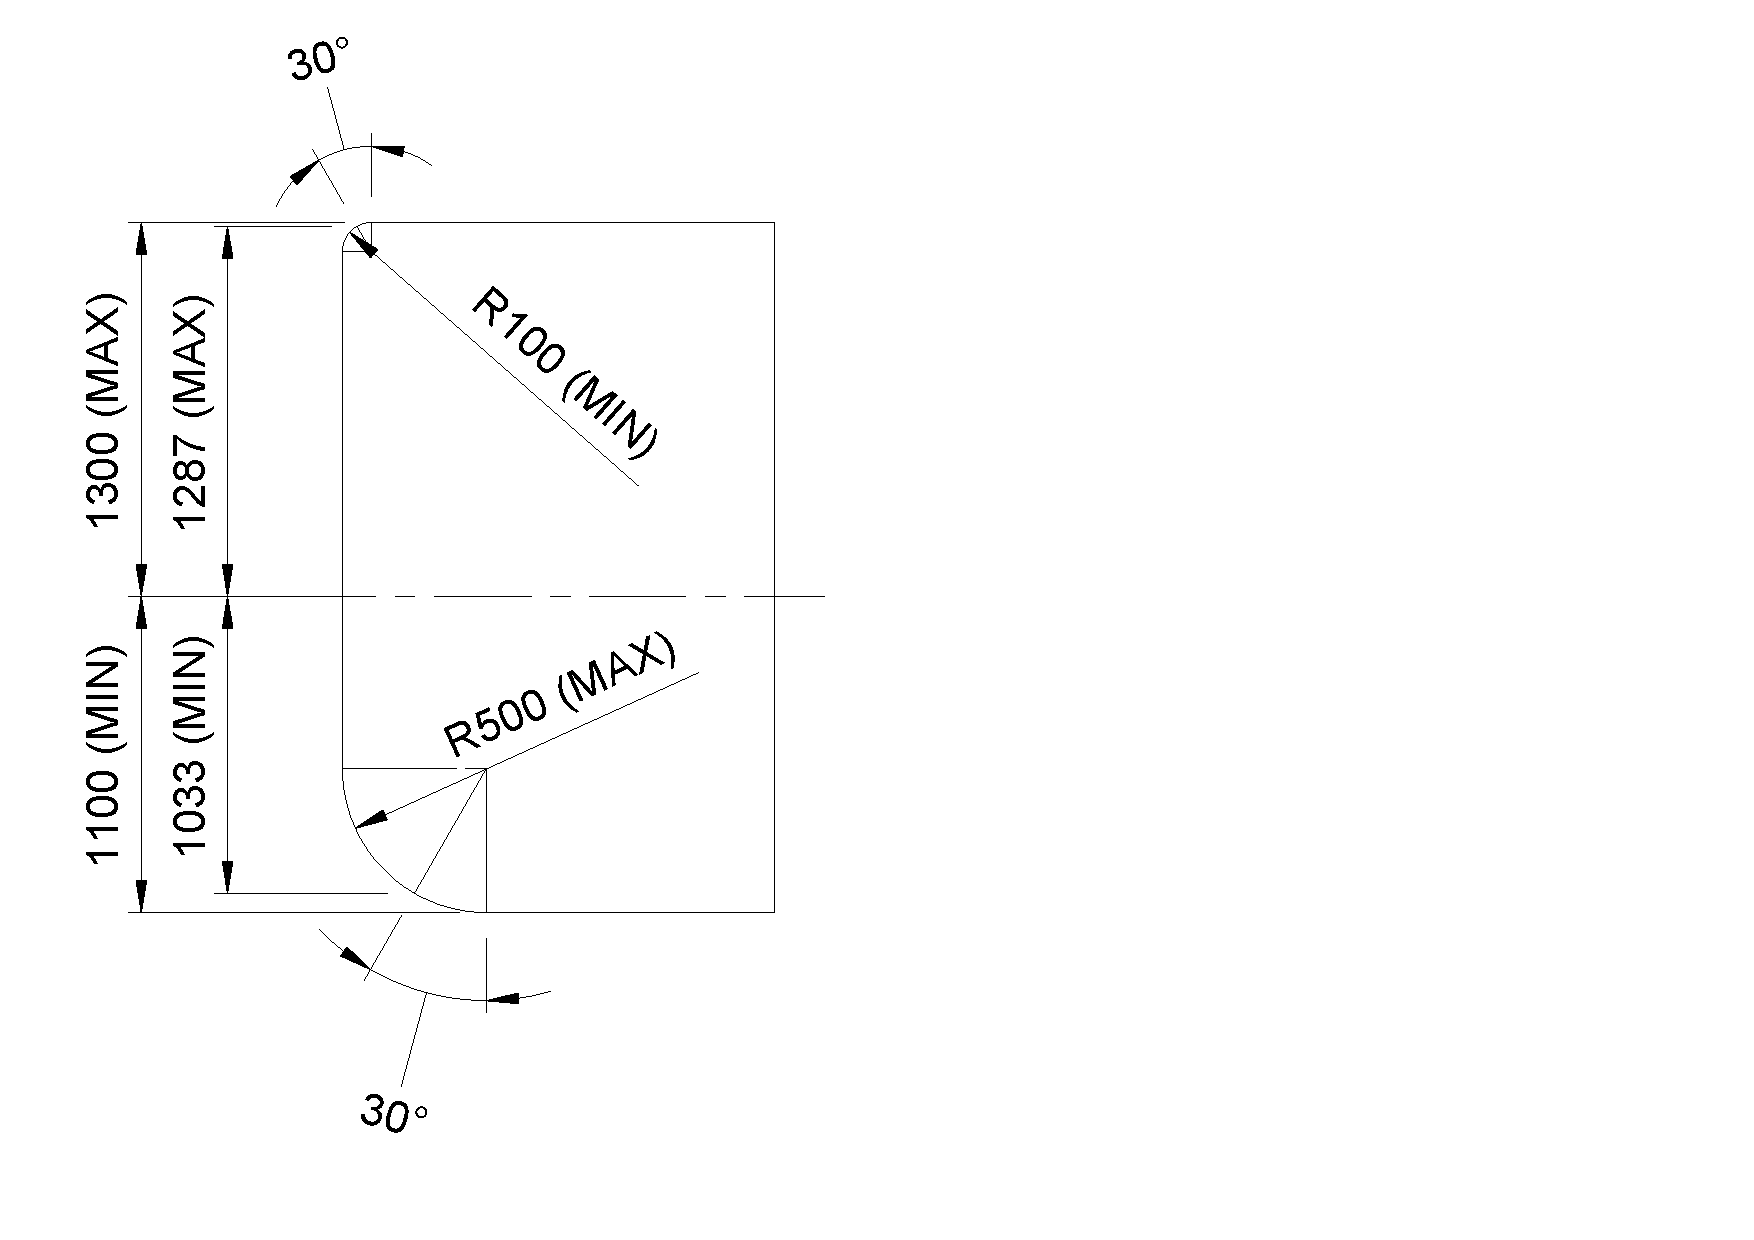
\includegraphics[width=0.5\textwidth]{fig/parameter-selection_vehicle-width_prime-mover}
	\caption{Parameter selection - prime mover frontal reference points}
	\label{figure:parameter-selection-vehicle-width}
\end{figure}
%----------------------------------------------
%      FIGURE
%----------------------------------------------

The trailer units were modelled as boxes without any curvature. The minimum width for a trailer was assumed to be 2400~mm, beyond which the deck width would become too small and unproductive.

A summary of the vehicle widths for all units is provided in Table~\ref{table:pr-vehicle-width}.

%----------------------------------------------
%      TABLE
%----------------------------------------------
\begin{table}[H]
	\centering\footnotesize
	\begin{threeparttable}

		\begin{tabulary}{\textwidth}{lccc}
			\toprule
			\textbf{Vehicle unit} & \textbf{Baseline (mm)} & \textbf{Min. (mm)} & \textbf{Max. (mm)} \\
			\midrule
			Prime mover (all) & 2495  & 2225  & 2600 \\
			Trailer (all) & 2600  & 2400  & 2600 \\
			\bottomrule
		\end{tabulary}

		\caption{Parameter range - vehicle width}
		\label{table:pr-vehicle-width}

		% 		\begin{tablenotes}
		% 			\item[1] %\tnote{1}
		% 		\end{tablenotes}

	\end{threeparttable}
\end{table}
%----------------------------------------------
%      TABLE
%----------------------------------------------

\subsection{Reference Point Height}\label{section-pr-ref-point-height}

Geometrical reference points at the forward-most outer and rearward-most outer of a \gls{hcv} are used to evaluating the amount of road space that a \gls{hcv} requires when performing road manoeuvres. The NTC rules \cite{NationalTransportCommission2008} state that if multiple points reside at the same reference point, the lowest of those points should be used.

The reference point height can range from ground height (for example a mud flap or sidewalls of a tyre) up to 4600~mm in the case of a car-carrier which is allowed an overall height of 4600~mm if approved as a \gls{pbs} safe vehicle \cite{AbnormalLoadTechnicalCommittee2014}. Thus, to encompass the worst case for all \glspl{hcv}, the reference points on each vehicle unit were varied from 0~mm to 4600~mm.

%      SUBSECTION
%----------------------------------------------
\subsection{Prime Mover and Trailer Wheelbase}\label{section:pr-wheelbase}

The range of wheelbases selected for each vehicle unit was determined using structural limitations in conjunction with Regulation 225 (b) regulating the maximum wheelbase for a vehicle unit and the previously mentioned Regulation 226 (2)(c) regulating the maximum rear overhang from the centre of the rearmost axle (see Section~\ref{section:pr-rear-overhang}).

Changing the wheelbase has a significant effect on the axle loadings and the baseline vehicles are based on PBS vehicles with axle loadings close to the legal limits. If the wheelbase were to be varied within a range where the axle loads remained legal, there would be minimal variation. This would remove insight into how the wheelbase impacts vehicle performance in the case of volume limited transport where the axle loadings have more scope to vary. Thus, for the selection of wheelbases, legal axle load requirements were ignored.

The minimum wheelbase was selected according to the following conditions:

\begin{enumerate}
	\item The resulting rear overhang reached 60\% of the wheelbase
	\item The hitch location coincides with the centre of the rearmost axle
	\item The vehicle configuration becomes unstable \footnote{Since the wheelbases are varied over a large range without altering the location of the payload, the vehicle model became unstable for short wheelbases. In these cases, the minimum wheelbase was increased in increments of 50~mm until the model became stable.}
\end{enumerate}

The maximum wheelbase was selected according to the following conditions:

\begin{enumerate}
	\item The maximum wheelbase for a semi-trailer of 10~m according to Regulation 225 (b)
	\item The edge of the tyre aligns with the edge of the chassis structure
	\item The edge of the tyre aligns with the pintle hitch connection point
\end{enumerate}

The maximum and minimum wheelbases are illustrated in Figures~\ref{figure:parameter-selection-wheelbase-quad-semi-trailer}~to~\ref{figure:parameter-selection-wheelbase-truck-and-dog}.

%----------------------------------------------
%      FIGURE
%----------------------------------------------
\begin{figure*}[!htbp]
	\centering
	\begin{subfigure}[t]{1\textwidth}
		\centering
		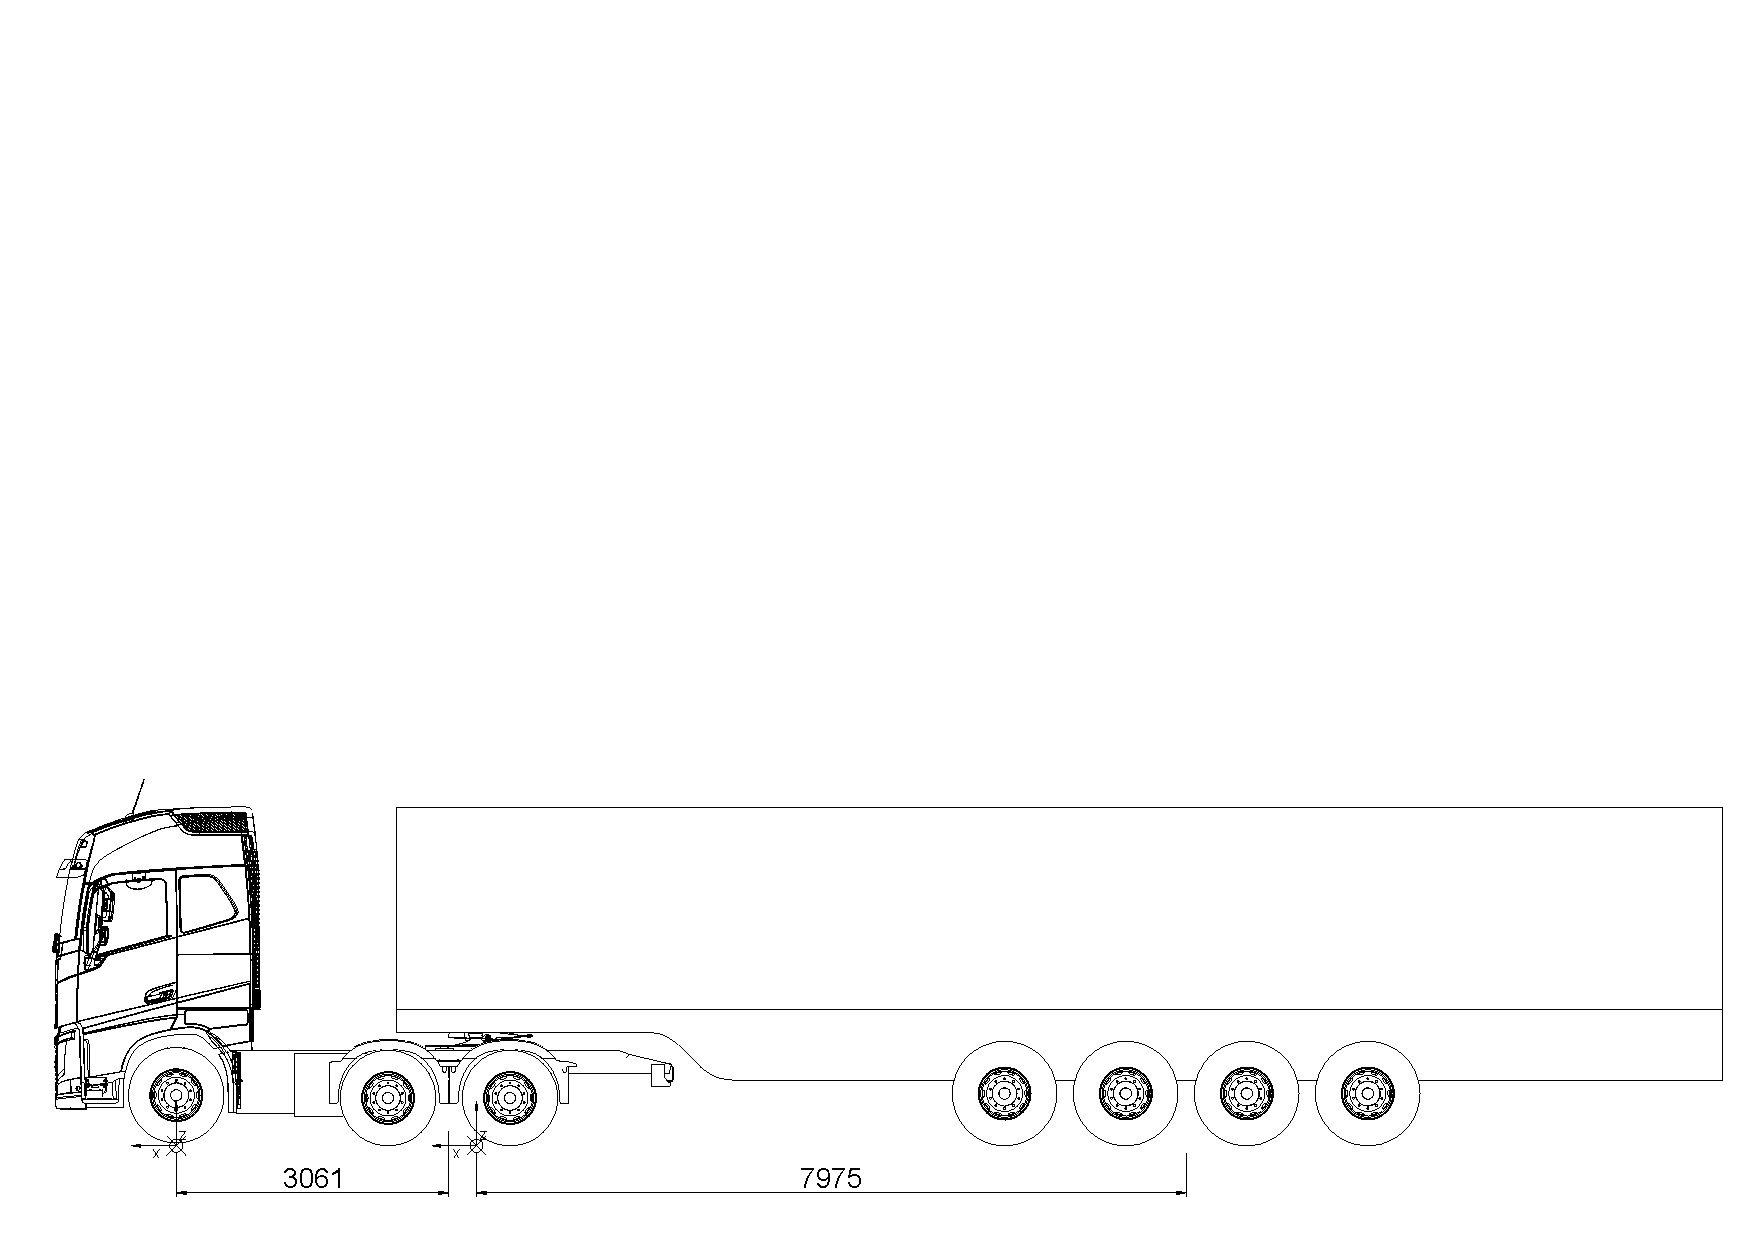
\includegraphics[width=1\textwidth]{fig/parameter-selection_wheelbase_min_quad-semi-trailer}
		\caption{Minimum wheelbase}
	\end{subfigure}%

	\begin{subfigure}[t]{1\textwidth}
		\centering
		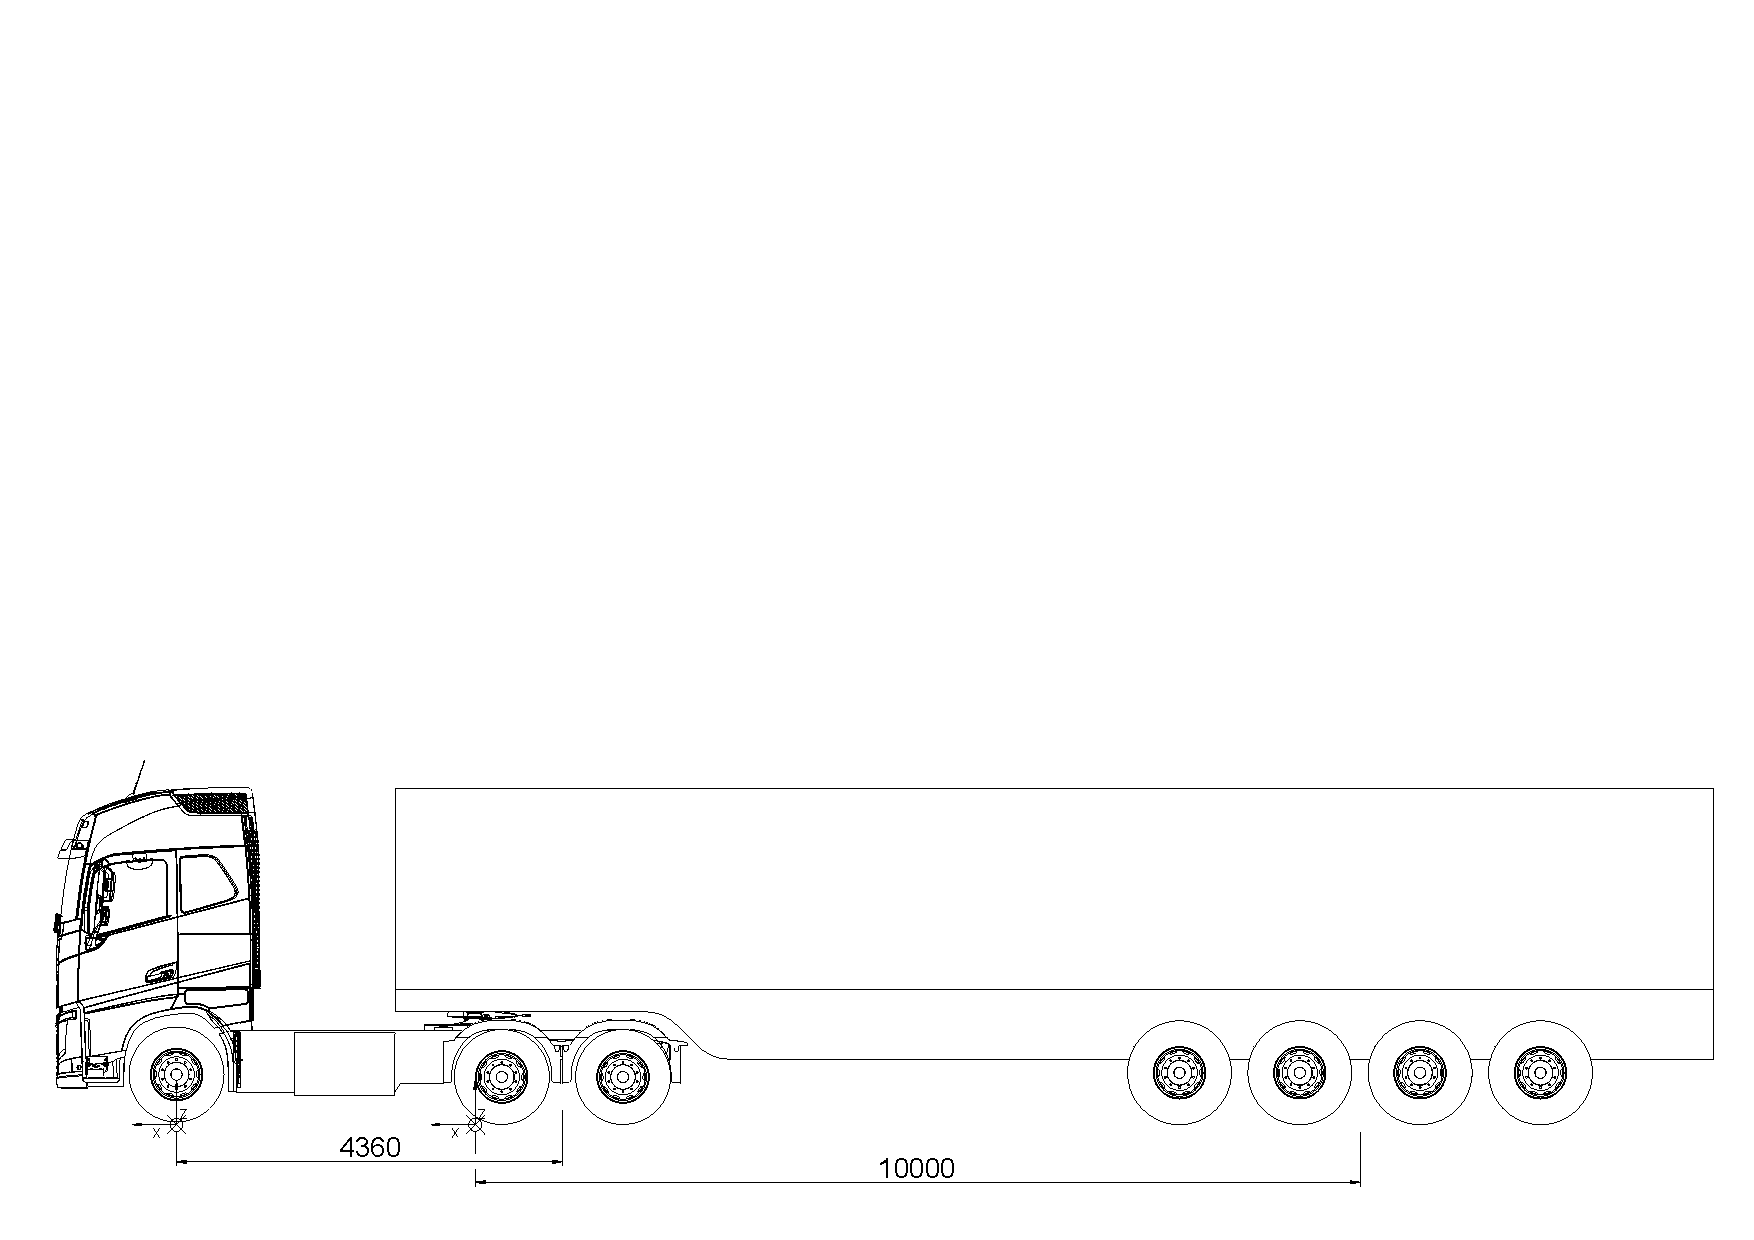
\includegraphics[width=1\textwidth]{fig/parameter-selection_wheelbase_max_quad-semi-trailer}
		\caption{Maximum wheelbase}
	\end{subfigure}

	\caption{Parameter selection - wheelbases for the quad semi-trailer combination}
	\label{figure:parameter-selection-wheelbase-quad-semi-trailer}
\end{figure*}
%----------------------------------------------
%      FIGURE
%----------------------------------------------

%----------------------------------------------
%      FIGURE
%----------------------------------------------
\begin{figure*}[!htbp]
	\centering
	\begin{subfigure}[t]{1\textwidth}
		\centering
		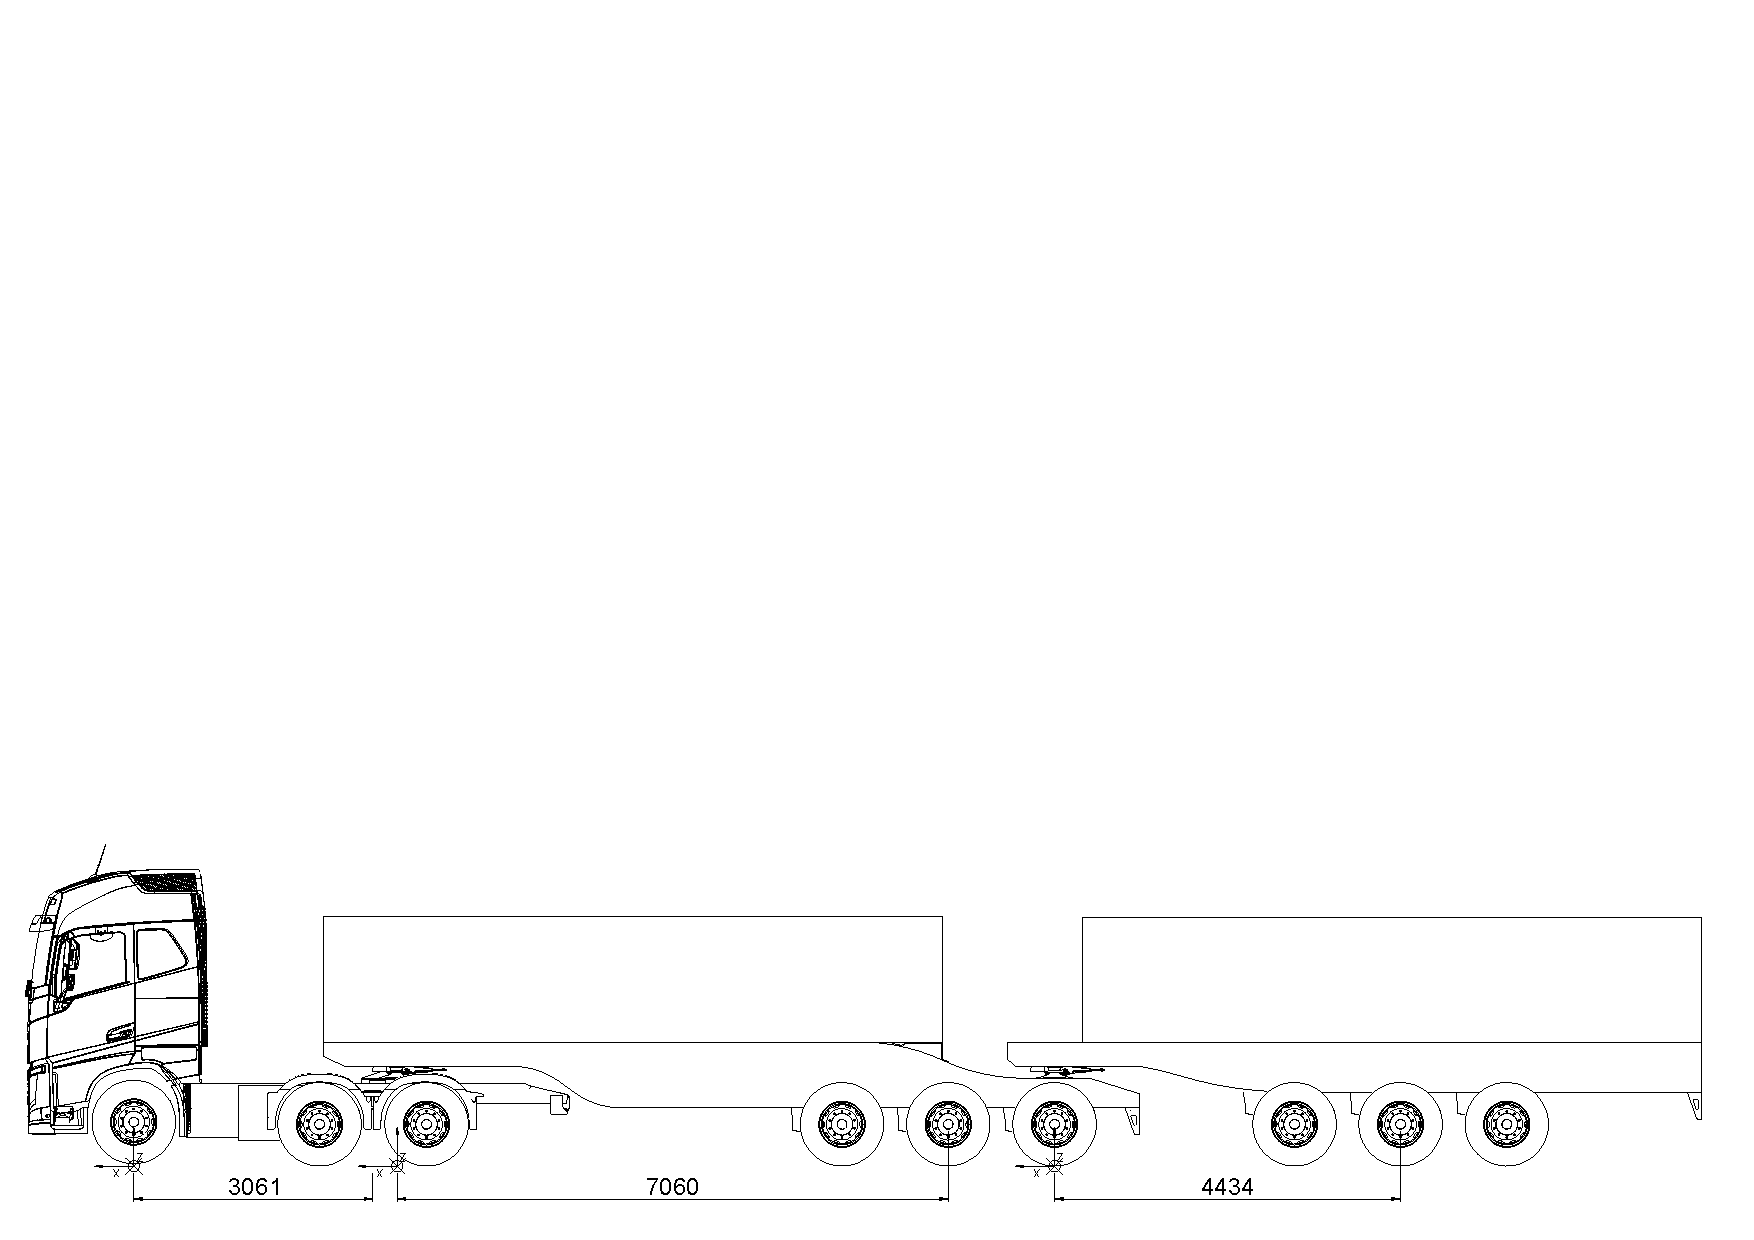
\includegraphics[width=1\textwidth]{fig/parameter-selection_wheelbase_min_b-double}
		\caption{Minimum wheelbase}
	\end{subfigure}%

	\begin{subfigure}[t]{1\textwidth}
		\centering
		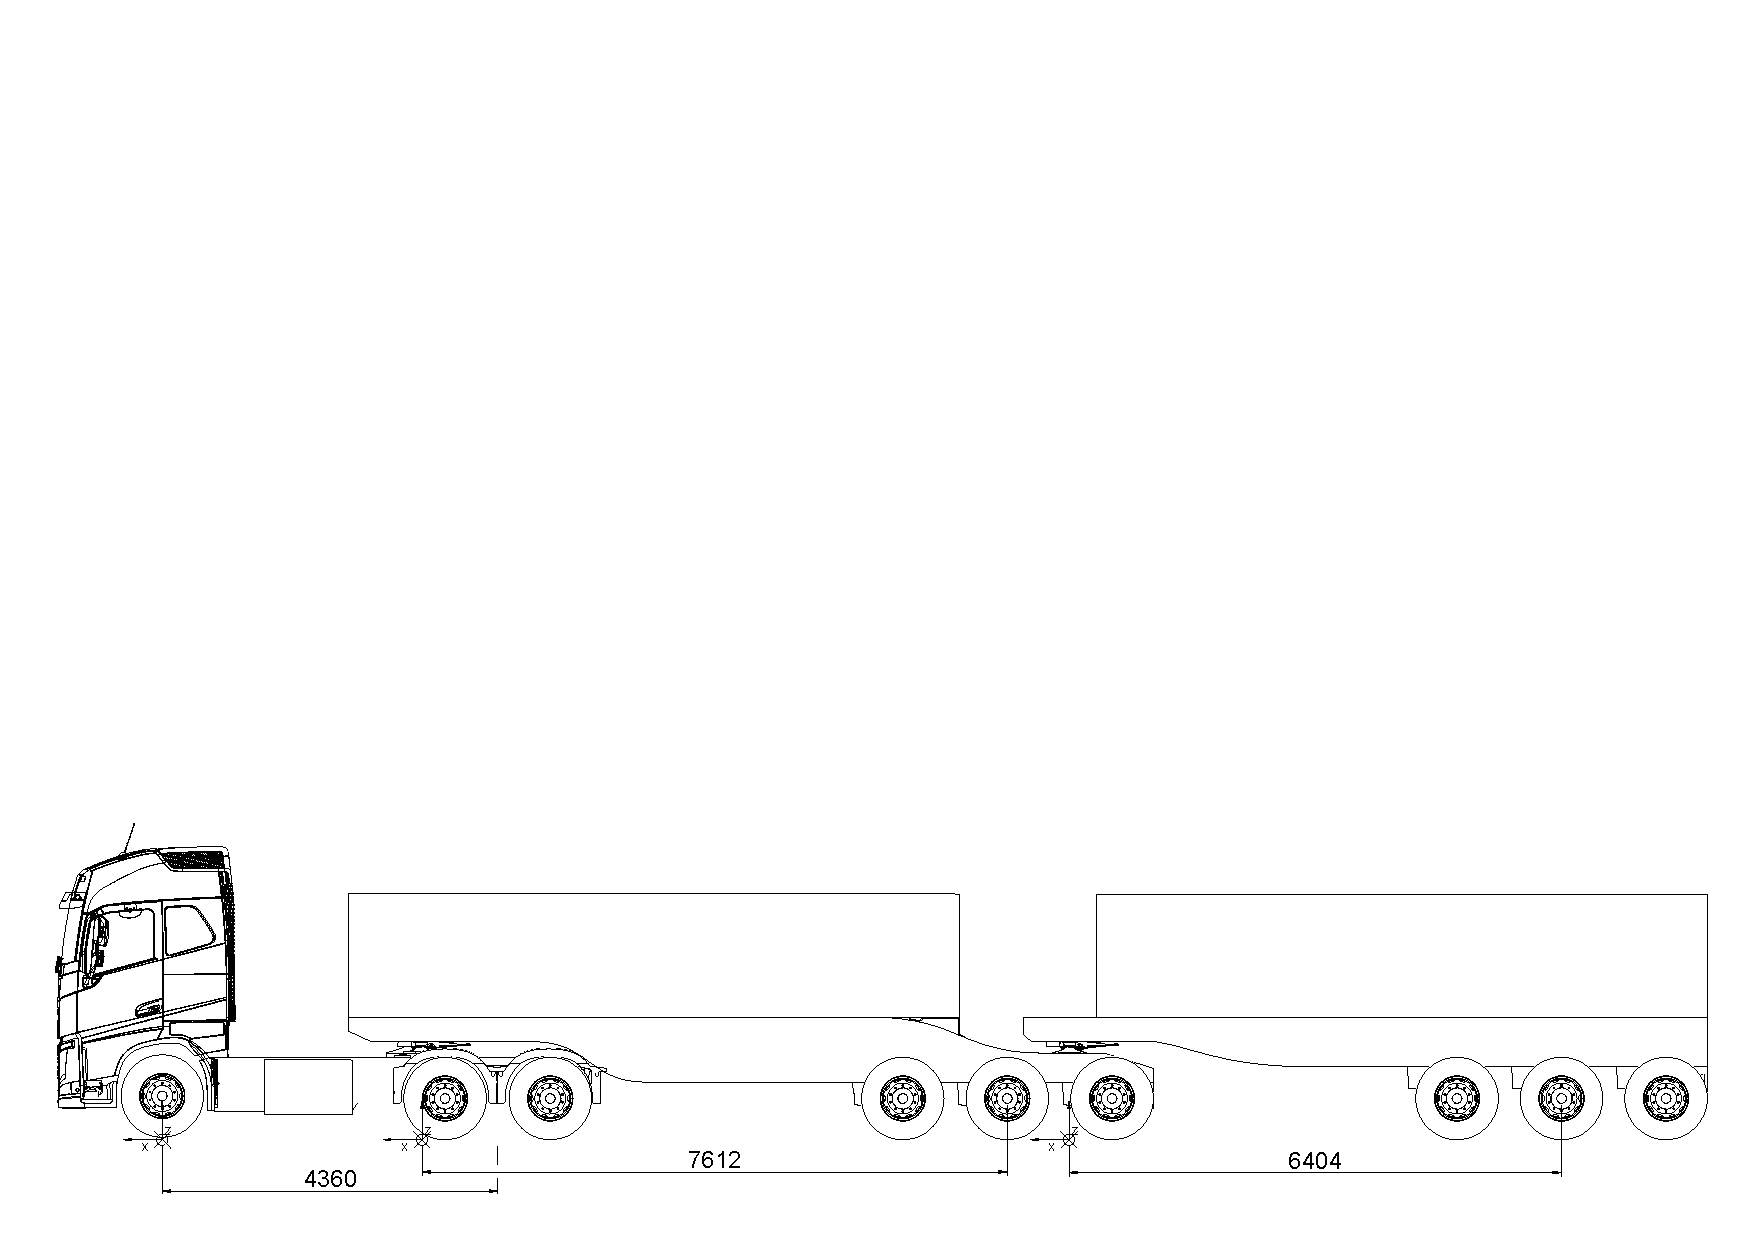
\includegraphics[width=1\textwidth]{fig/parameter-selection_wheelbase_max_b-double}
		\caption{Maximum wheelbase}
	\end{subfigure}

	\caption{Parameter selection - wheelbases for the tridem interlink combination}
	\label{figure:parameter-selection-wheelbase-b-double}
\end{figure*}
%----------------------------------------------
%      FIGURE
%----------------------------------------------

%----------------------------------------------
%      FIGURE
%----------------------------------------------
\begin{figure*}[!htbp]
	\centering
	\begin{subfigure}[t]{1\textwidth}
		\centering
		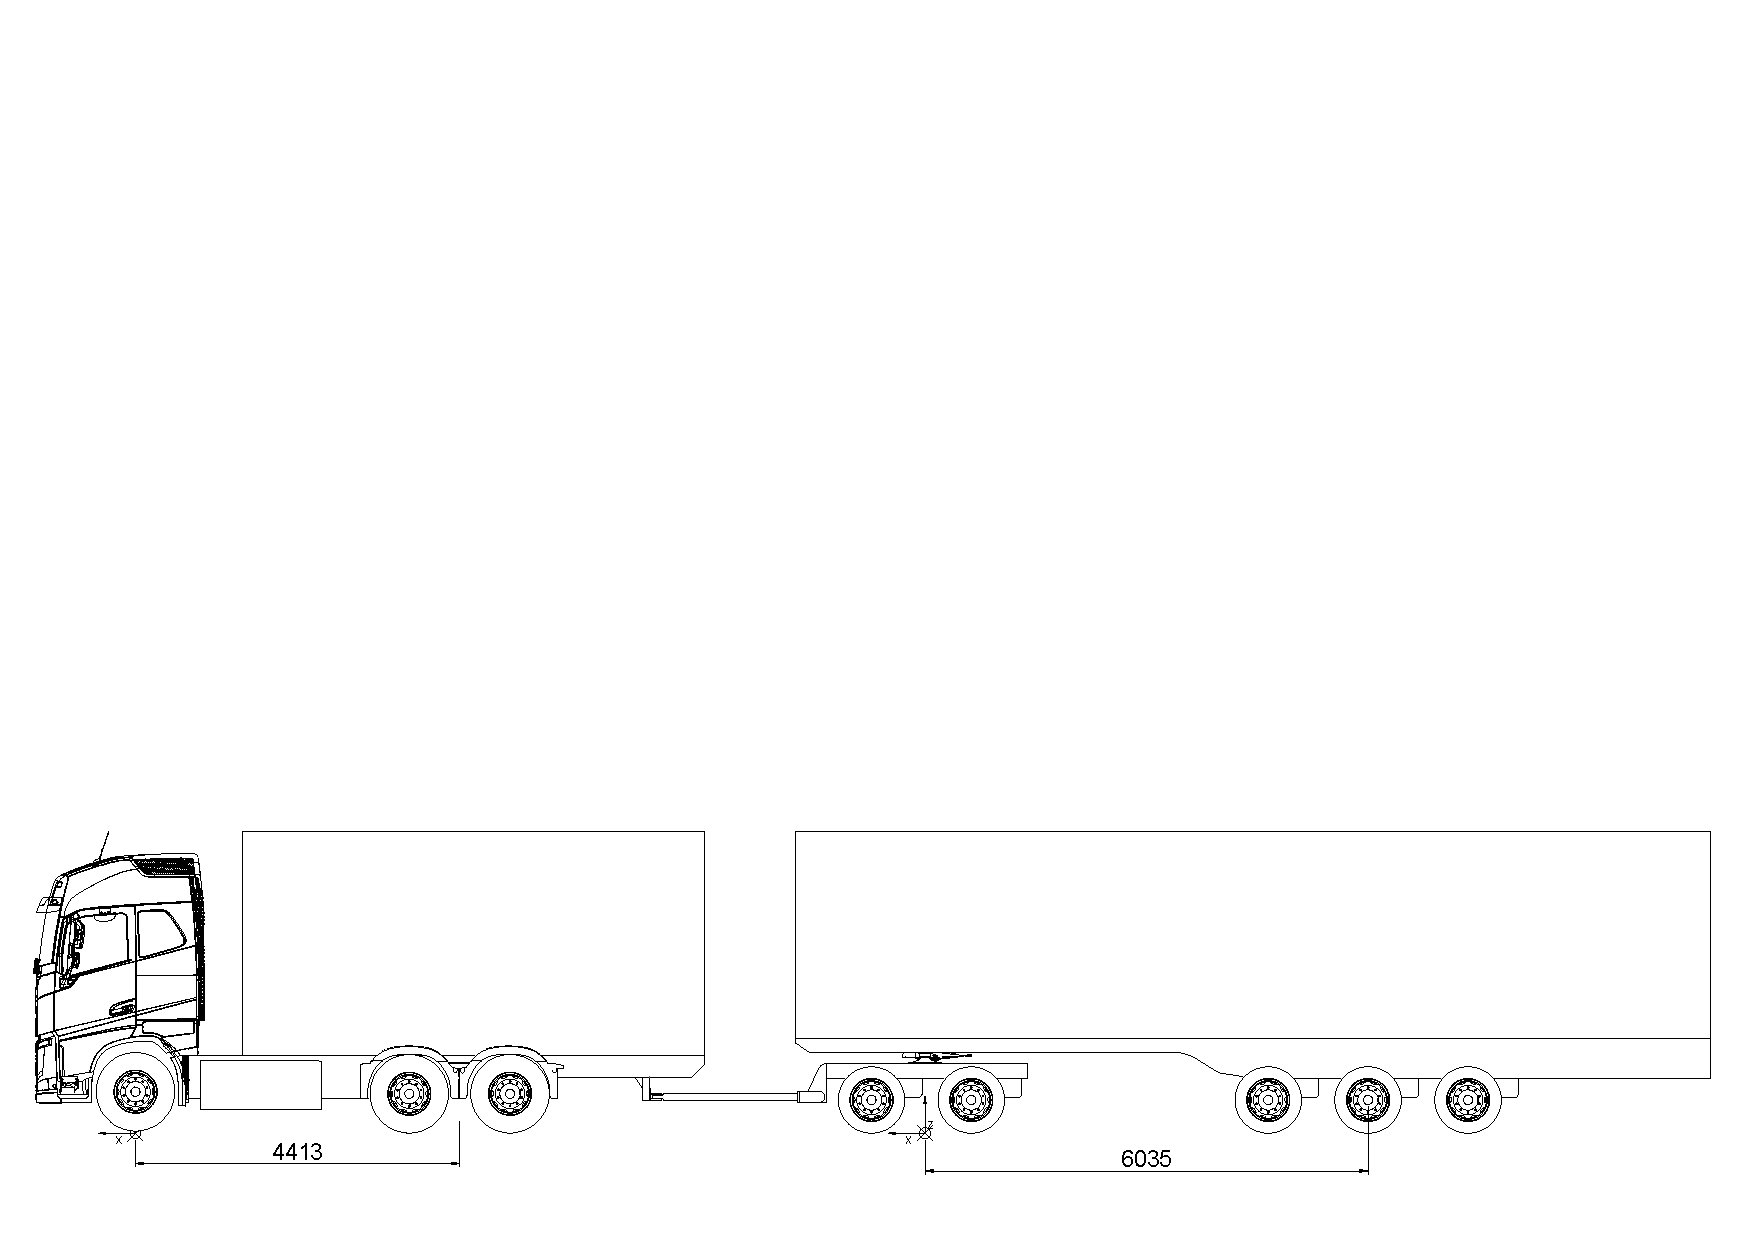
\includegraphics[width=1\textwidth]{fig/parameter-selection_wheelbase_min_truck-and-dog}
		\caption{Minimum wheelbase}
	\end{subfigure}%

	\begin{subfigure}[t]{1\textwidth}
		\centering
		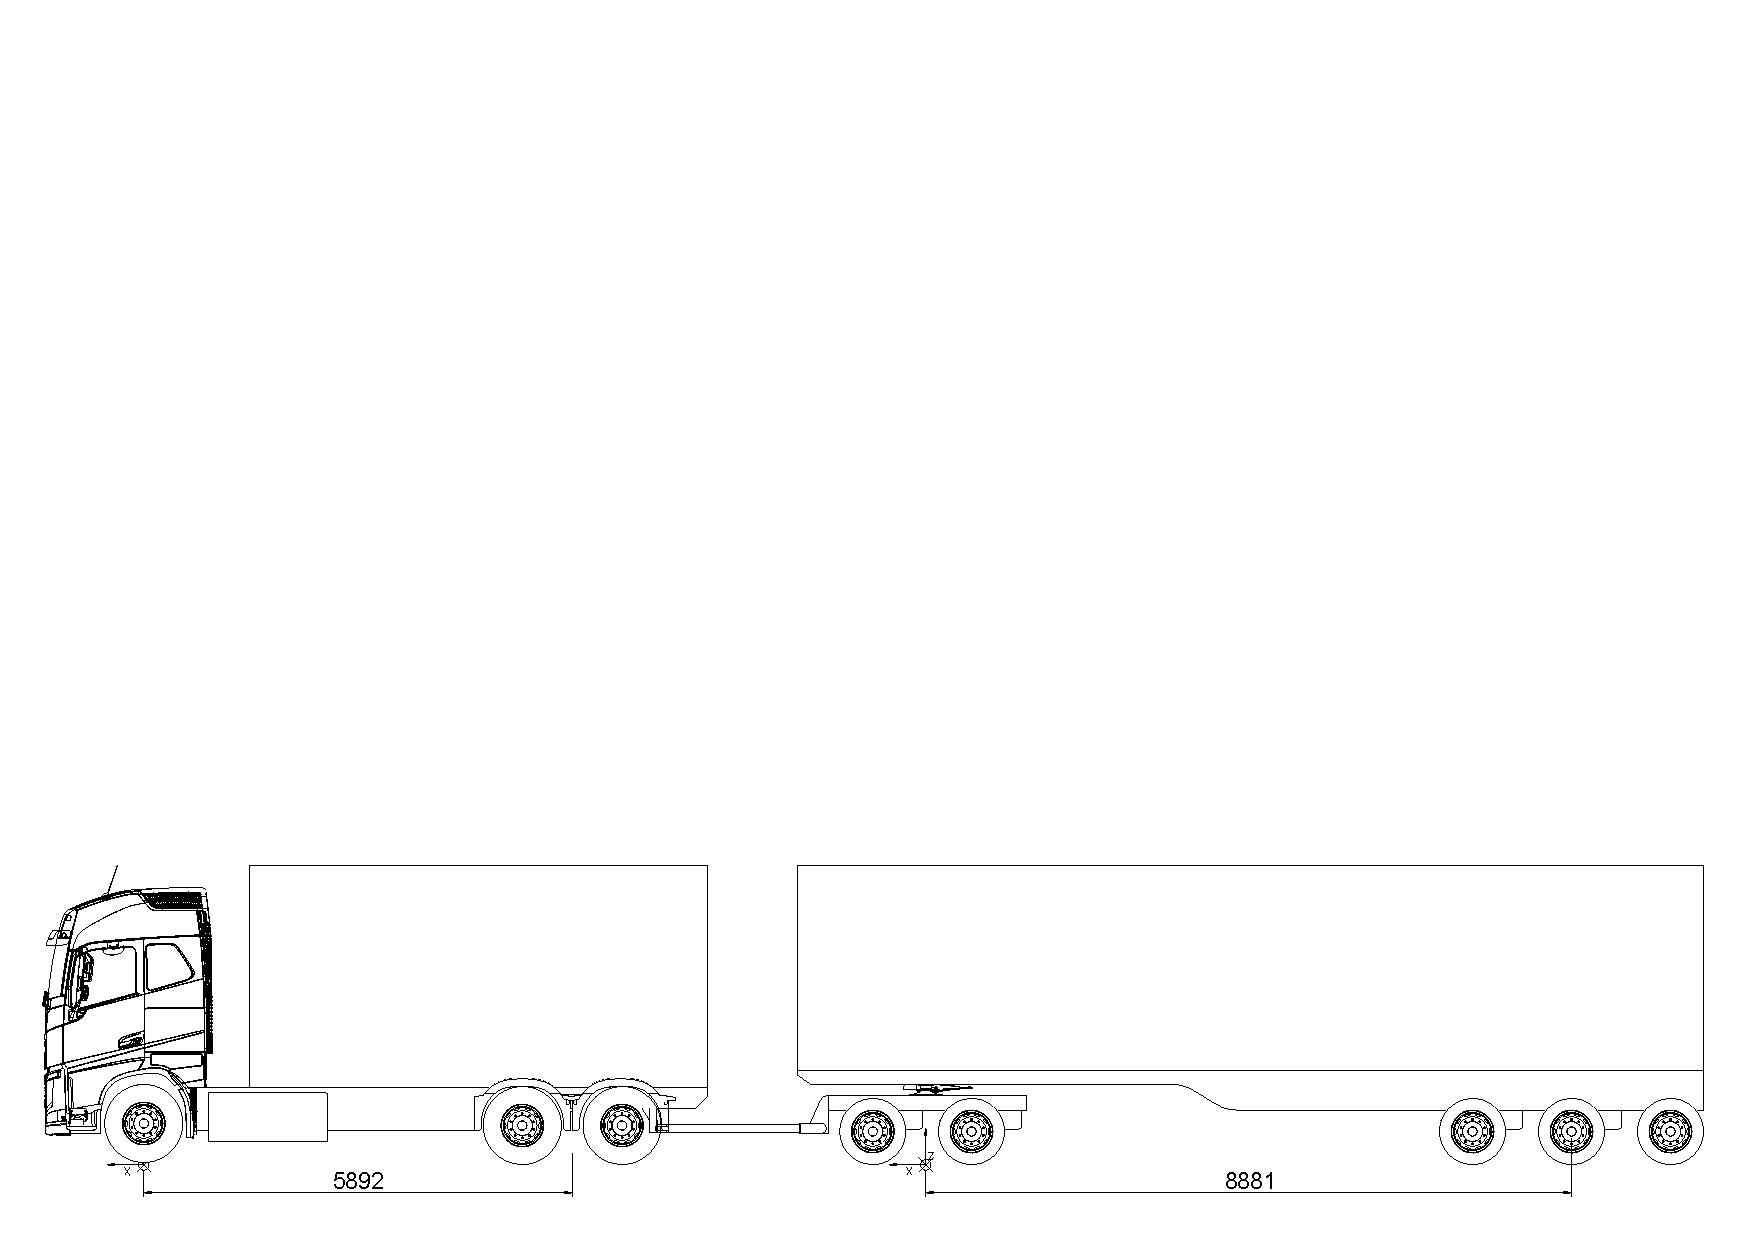
\includegraphics[width=1\textwidth]{fig/parameter-selection_wheelbase_max_truck-and-dog}
		\caption{Maximum wheelbase}
	\end{subfigure}

	\caption{Parameter selection - wheelbases for the rigid drawbar combination}
	\label{figure:parameter-selection-wheelbase-truck-and-dog}
\end{figure*}
%----------------------------------------------
%      FIGURE
%----------------------------------------------

A summary of the range of wheelbases evaluated for each vehicle unit is included in Table~\ref{table:parameter-range-wheelbase}.

%----------------------------------------------
%      TABLE - UPDATED TO NEW RANGES
%----------------------------------------------
\begin{table}[H]
	\centering\footnotesize
	\begin{threeparttable}

		\begin{tabulary}{\textwidth}{lcccll}
			\toprule
			\textbf{Vehicle unit} & \textbf{Baseline (mm)} & \textbf{Min. (mm)} & \textbf{Max. (mm)} & \textbf{Rationale min.} & \textbf{Rationale max.} \\
			\midrule
            Truck tractor & 3885  & 3061  & 4360  & Regulation 226 (2)(c) & Structural \\
            Rigid truck & 5285  & 4413  & 5892  & Regulation 226 (2)(c) & Structural \\
            Quad semi-trailer & 10000 & 7975  & 10000 & Model stability & Regulation 225 (b) \\
            Tridem interlink leader & 7420  & 7060  & 7612  & Hitch location & Structural \\
            Tridem interlink follower & 5950  & 4434  & 6404  & Model stability & Structural \\
            Tridem semi-trailer & 8255  & 6035  & 8881  & Model stability & Structural \\
			\bottomrule
		\end{tabulary}

		\caption{Parameter range - wheelbase}
		\label{table:parameter-range-wheelbase}

		% 		\begin{tablenotes}
		% 			\item[1] %\tnote{1}
		% 		\end{tablenotes}

	\end{threeparttable}
\end{table}
%----------------------------------------------
%      TABLE
%----------------------------------------------

%      SUBSECTION
%----------------------------------------------
\subsection{Dolly Wheelbase (Drawbar Length)}\label{section:drawbar-length}

The range for the dolly wheelbase was determined according to the range of allowed drawbar lengths. Regulation 222 (2b) states the length of an underslung drawbar may exceed 2~m in length if the distance between the two vehicles does not exceed 2.5~m. Using this regulation, the maximum allowed drawbar length is 3451~mm as shown in Figure~\ref{figure:maximum-drawbar-length-according-to-regulation-222-2b}.

%----------------------------------------------
%      FIGURE
%----------------------------------------------
\begin{figure}[H]
	\centering
	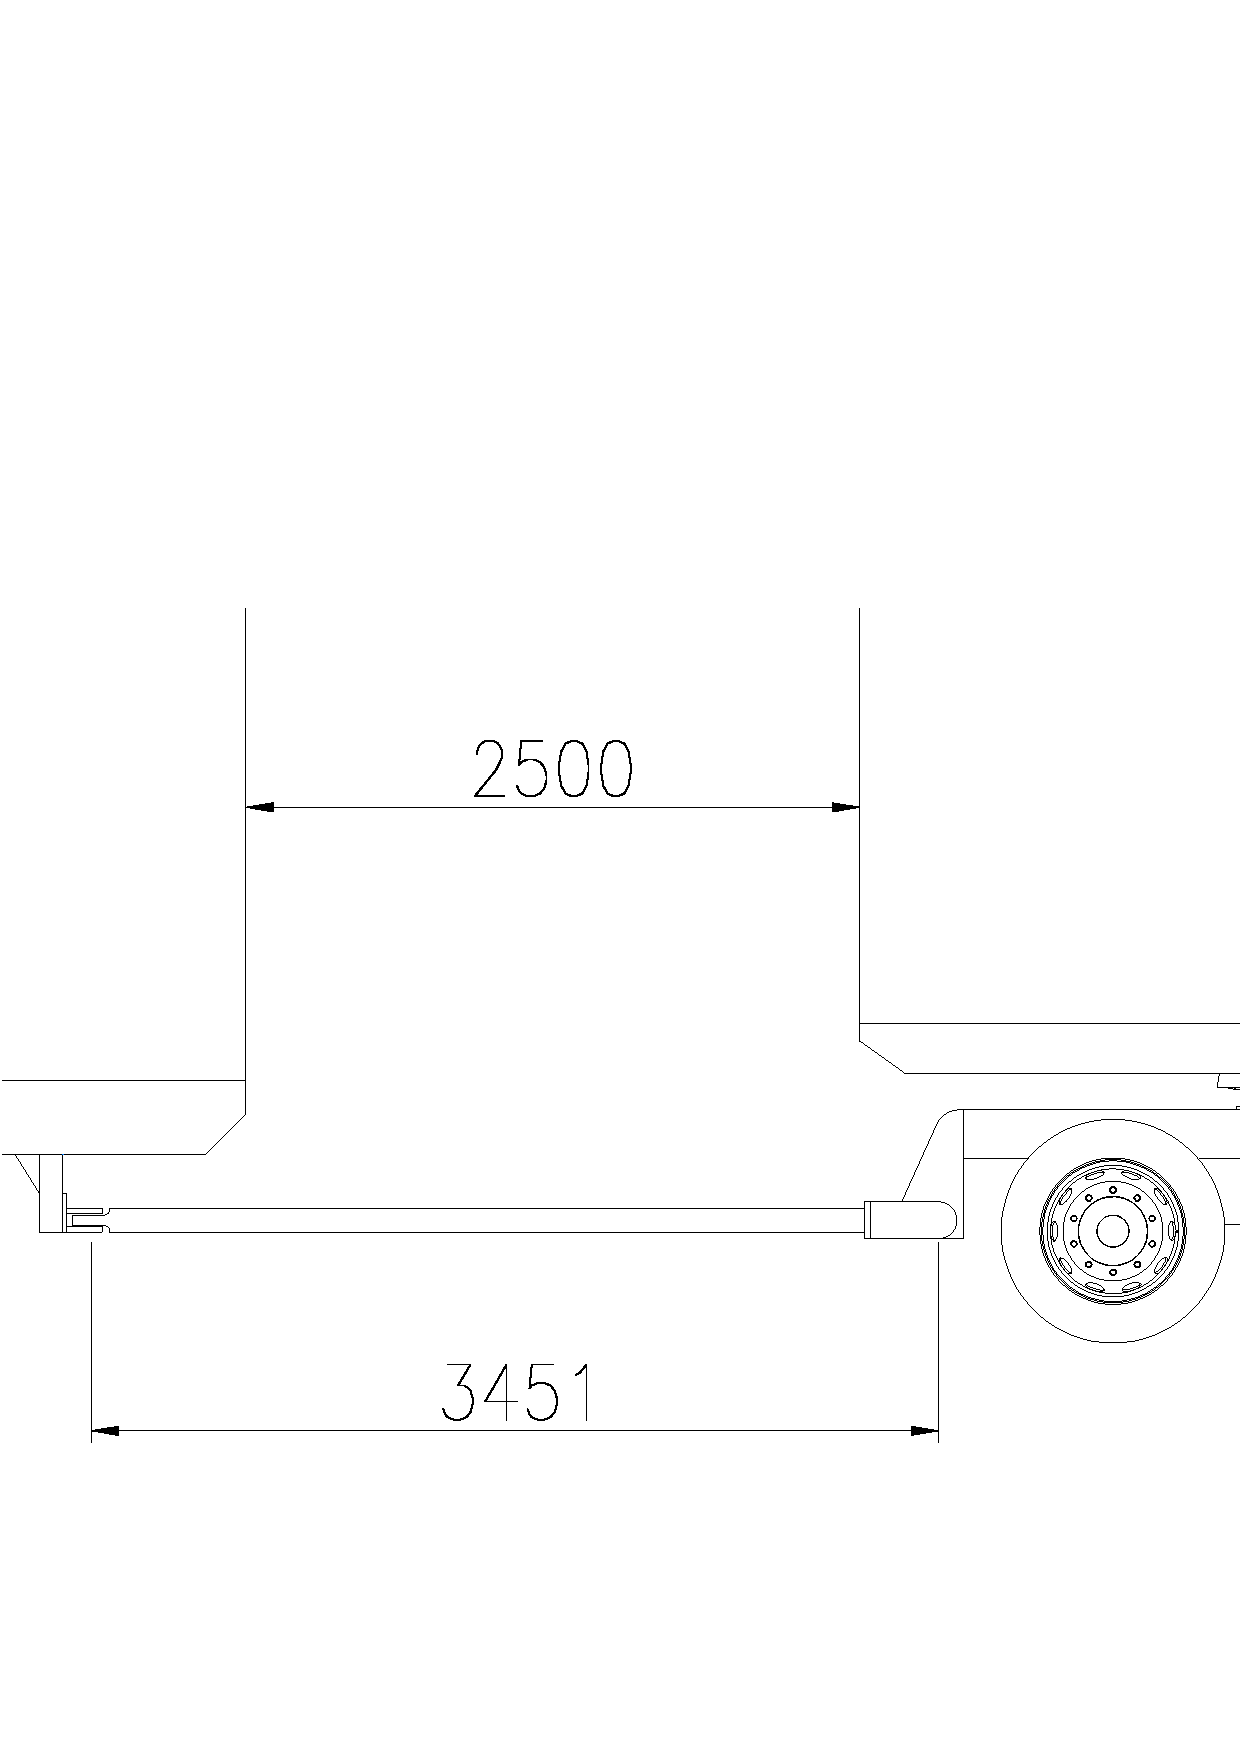
\includegraphics[width=0.5\textwidth]{fig/baseline-pintle-hitch-maximum-length}
	\caption{Maximum drawbar length according to regulation 222 (2b)}
	\label{figure:maximum-drawbar-length-according-to-regulation-222-2b}
\end{figure}
%----------------------------------------------
%      FIGURE
%----------------------------------------------

The minimum drawbar length was chosen such that there would be a 50~mm clearance between the trailer swing radius and the rigid truck chassis resulting in a minimum drawbar length of 1429~mm as shown in Figure~\ref{figure:minimum-drawbar-length}.

%----------------------------------------------
%      FIGURE
%----------------------------------------------
\begin{figure}[H]
	\centering
	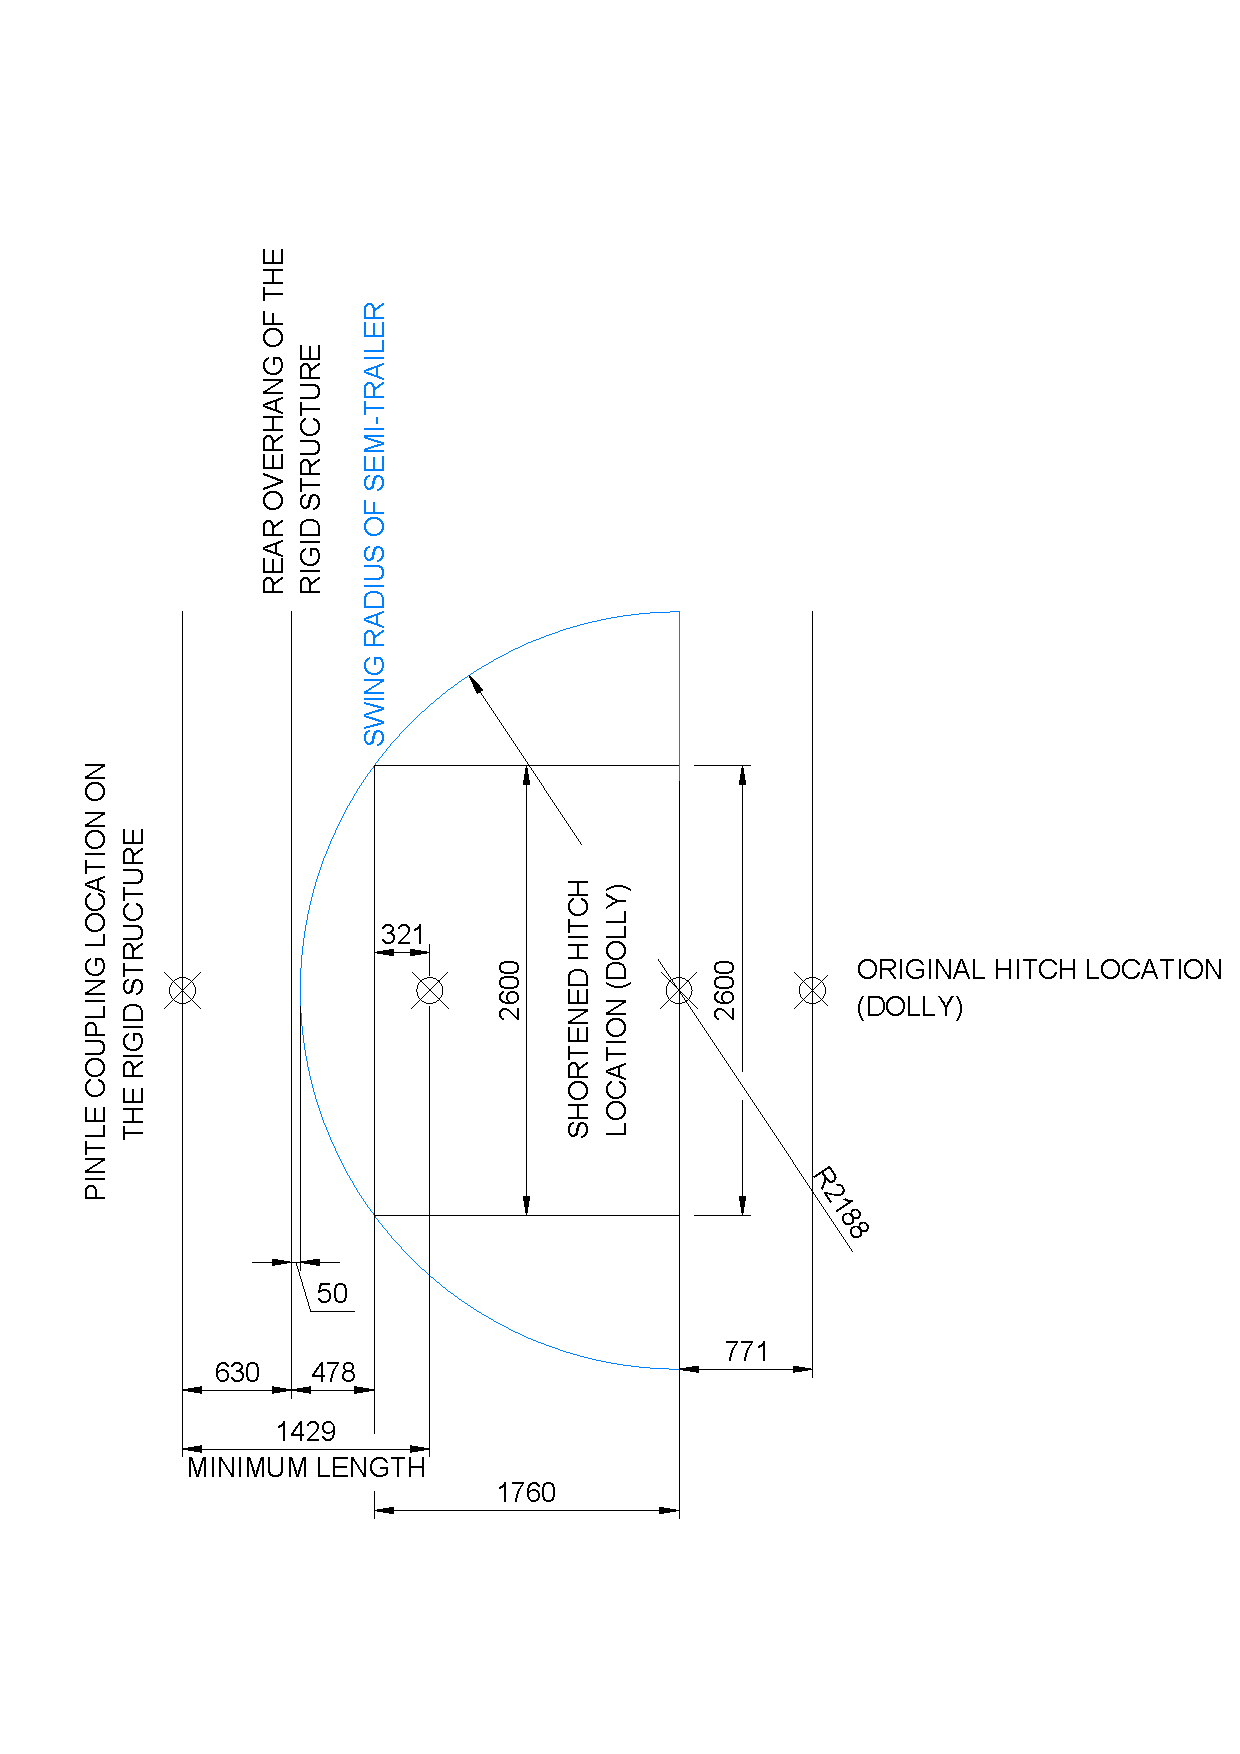
\includegraphics[width=0.7\textwidth]{fig/baseline-pintle-hitch-minimum-length}
	\caption{Minimum drawbar length}
	\label{figure:minimum-drawbar-length}
\end{figure}
%----------------------------------------------
%      FIGURE
%----------------------------------------------

%----------------------------------------------
%      TABLE - UPDATED TO NEW RANGES
%----------------------------------------------
\begin{table}[H]
	\centering\footnotesize
	\begin{threeparttable}

		\begin{tabulary}{\textwidth}{lcccll}
			\toprule
			\textbf{Details} & \textbf{Baseline (mm)} & \textbf{Min. (mm)} & \textbf{Max. (mm)} & \textbf{Rationale Min.} & \textbf{Rationale Max.} \\

			\midrule
			Drawbar length & 2200  & 1429  & 3451  & Structural & Regulation 222 (3) \\
			Wheelbase      & 3590  & 2819  & 4841  & Drawbar length & Drawbar length \\
			\bottomrule

		\end{tabulary}

		\caption{Parameter range - dolly wheelbase and drawbar length}
		\label{table:parameter-range-dolly-pintle-hitch-length}

		%\begin{tablenotes}
		%\item[1] %\tnote{1}
		%\end{tablenotes}

	\end{threeparttable}
\end{table}
%----------------------------------------------
%      TABLE
%----------------------------------------------

%      SUBSECTION
%----------------------------------------------
\subsection{Axle Spacing}\label{section:pr-axle-spacing}

The only publicly available legislation that could be found that explicitly governs axle spacing is the Canadian legislation (British Columbia) \cite{StatutesRegulations} which states that axle spacing should range between 1.2~m to 1.85~m and limits drive axles to a maximum spacing of 1.4~m. This legislation allowed a larger range of variation than typically observed in South Africa (trailer axle spacing of 1360~mm and drive axle spacing of 1400~mm are commonly observed in PBS assessments conducted in South Africa) and was thus deemed to represent a suitable and conservative range of variation for axle spacing.

The drive axle group spacing was varied from 1.2~m to 1.4~m. It was practical to vary all trailer axle group spacing from 1.2~m to 1.85~m as there were no interference's between adjacent axles. The dolly axle group was varied from 1.2~m to 1.8~m since the edge of the front tyre interferes with the pintle hitch position at larger spacing.

The resulting range of axle spacing evaluated for each vehicle unit is summarised in Table~\ref{table:pr-axle-spacing}.

%----------------------------------------------
%      TABLE
%----------------------------------------------
\begin{table}[H]
	\centering\footnotesize
	\begin{threeparttable}

		\begin{tabulary}{\textwidth}{lcccll}
			\toprule
			\textbf{Vehicle unit} & \textbf{Baseline (mm)} & \textbf{Min. (mm)} & \textbf{Max. (mm)} & \textbf{Rationale Min.} & \textbf{Rationale Max.} \\
			\midrule
			Truck tractor & 1370  & 1200  & 1400  & Legislation & Legislation \\
			Rigid truck & 1370  & 1200  & 1400  & Legislation & Legislation \\
			Quad Semi-trailer & 1360  & 1200  & 1850  & Legislation & Legislation \\
			Tridem interlink leader & 1360  & 1200  & 1850  & Legislation & Legislation \\
			Tridem interlink follower & 1360  & 1200  & 1850  & Legislation & Legislation \\
			Tridem semi-trailer & 1360  & 1200  & 1850  & Legislation & Legislation \\
			Dolly & 1360  & 1200  & 1800  & Legislation & Structural limitation \\
			\bottomrule
		\end{tabulary}

		\caption{Parameter range - axle spacing}
		\label{table:pr-axle-spacing}

		%\begin{tablenotes}
		%\item[1] %\tnote{1}
		%\end{tablenotes}

	\end{threeparttable}
\end{table}
%----------------------------------------------
%      TABLE
%----------------------------------------------

%      SUBSECTION
%----------------------------------------------
\subsection{Hitch Longitudinal Location}\label{section:pr-hitch-long-locations}

Common longitudinal hitch positions on tractors were measured by Fancher et al. \cite{Fancher1986}. Hitch positions were measured relative to the centre of the rear axle or rear axle group of between 0" and 24" (610 mm) forward of the rear axle or centre of the tandem axle group.

\textbf{Truck-tractor (5th wheel):}
Longitudinal positions for the tractor hitch position provided by the OEM\footnote{Permission was not received to mention the name of the OEM} correlated well with the data from Fancher et al. with hitch locations from 0~mm to 685~mm forward of the drive axle tandem group. The \gls{oem} range was evaluated for the largest range of possible locations.

\textbf{Rigid truck (pintle hitch):}
It was assumed that the pintle hitch could be mounted on the rigid truck chassis from the edge of the chassis up until the hitch position reached 50~mm from the rearmost drive tyre.

\textbf{Tridem interlink leader (5th wheel):}
The location of the hitch on the tridem interlink leader trailer is largely governed by the limited space on the chassis. It was graphically determined that limits of -380 and +620 from the baseline position would be possible with minimal modifications to the chassis design. The hitch centreline was not allowed further rear than the centreline of the last axle in the axle group. An illustration showing the graphically determined baseline, minimum and maximum position is shown in Figure~\ref{figure:b-double-5th-wheel-hitch-locations}.

%----------------------------------------------
%      FIGURE
%----------------------------------------------
\begin{figure}[H]
	\centering
	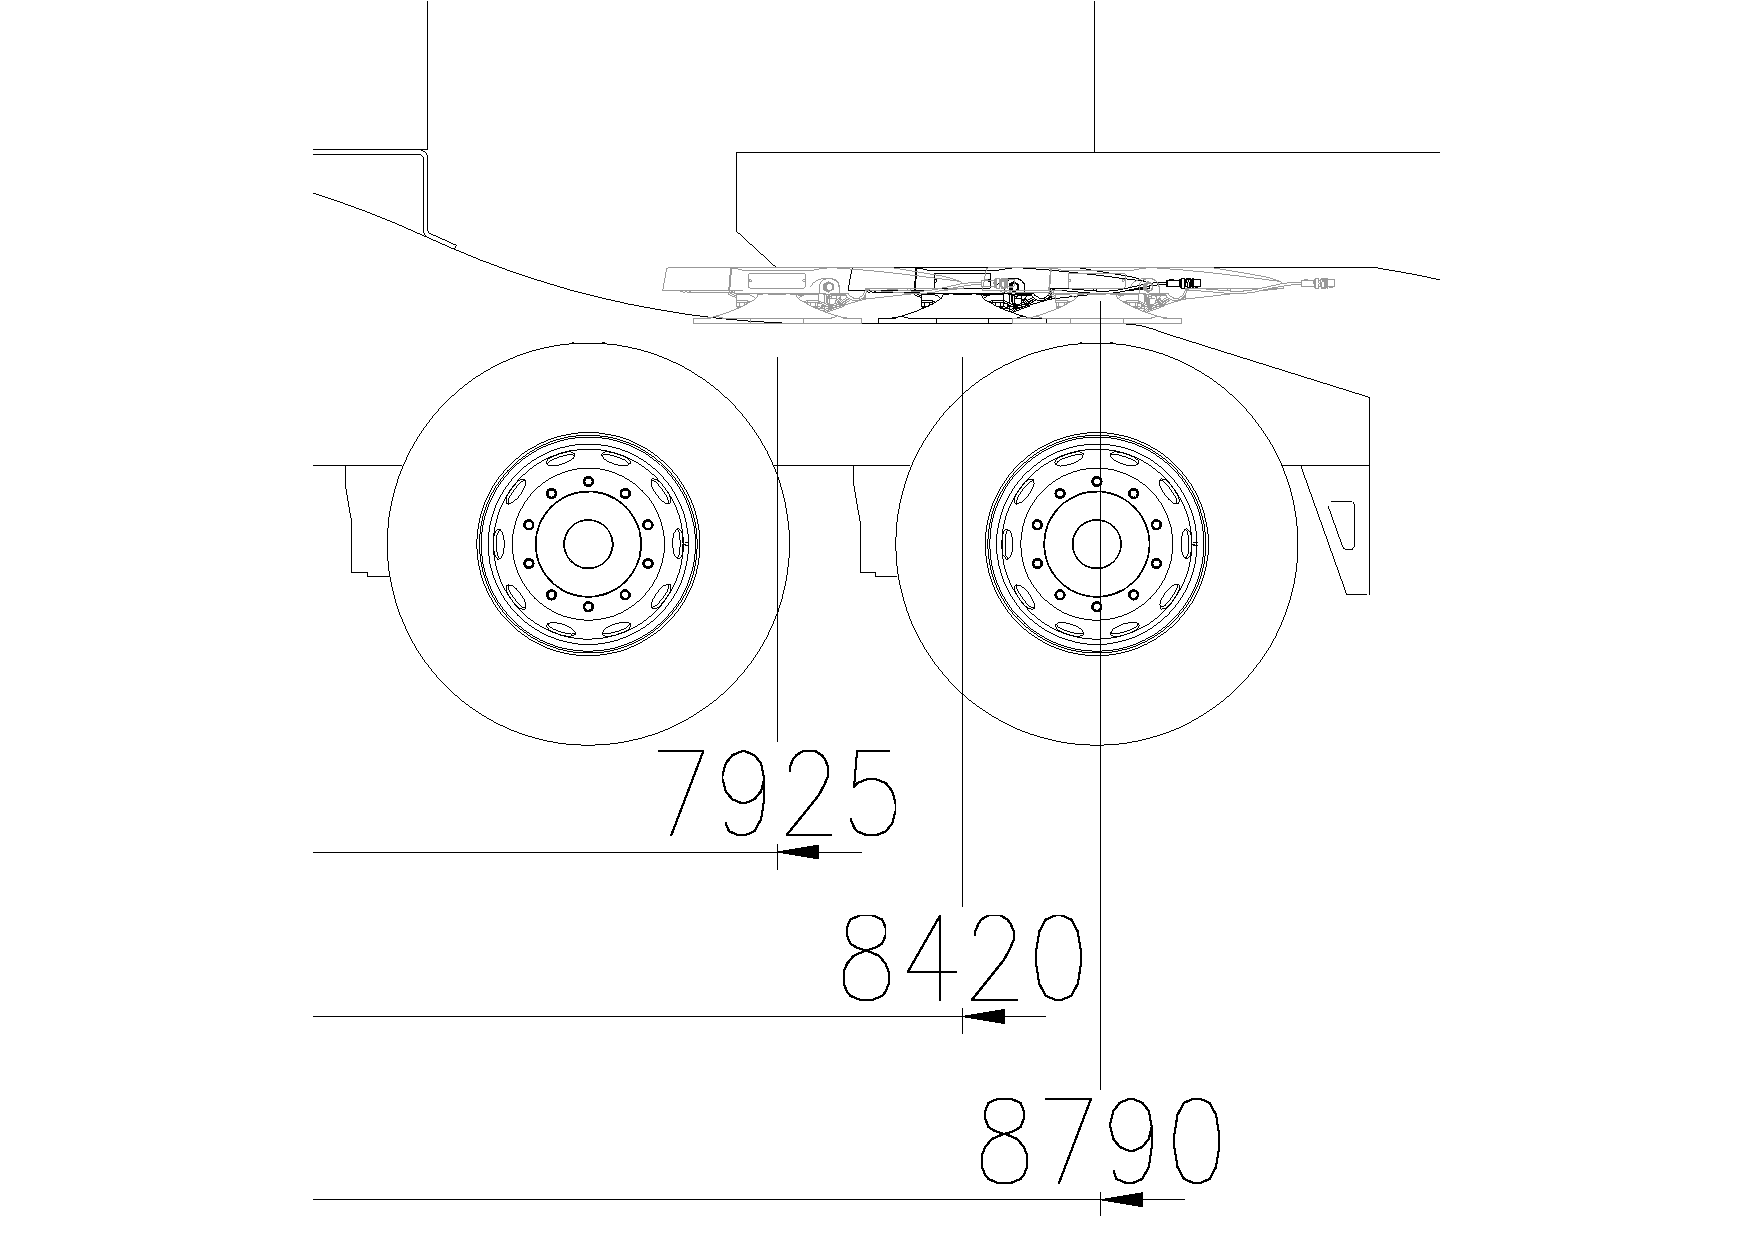
\includegraphics[width=0.5\textwidth]{fig/baseline_b-double_hitch-locations}
	\caption{5th wheel longitudinal locations for the tridem interlink leader trailer}
	\label{figure:b-double-5th-wheel-hitch-locations}
\end{figure}
%----------------------------------------------
%      FIGURE
%----------------------------------------------

\textbf{Rigid drawbar combination dolly (5th wheel):}
The typical 5th wheel location should be located at or near the centre of the dolly to avoid instabilities, it was hence assumed that the dolly 5th wheel location could only be moved +/-200 mm from the centre of the dolly axle group.

A summary of the evaluated hitch locations as discussed above is included in Table~\ref{table:pr-longitudinal-hitch-locations}.

%----------------------------------------------
%      TABLE - UPDATED TO NEW RANGES
%----------------------------------------------
\begin{table}[H]
	\centering\footnotesize
	\begin{threeparttable}

		\begin{tabulary}{\textwidth}{lccc}
			\toprule
			\textbf{Vehicle unit} & \textbf{Baseline (mm)\tnote{1}} & \textbf{Min. (mm)} & \textbf{Max. (mm)} \\
			\midrule
            Truck tractor & -3375 & -3200 & -3885 \\
            Rigid truck & -7115 & -6558 & -7860 \\
            Tridem interlink leader & -8420 & -7925 & -8780 \\
            Dolly & -3639 & -3385 & -3785 \\
			\bottomrule
		\end{tabulary}

		\caption{Parameter range - longitudinal hitch locations}
		\label{table:pr-longitudinal-hitch-locations}

		\begin{tablenotes}
			\item[1] SAE up co-ordinate system and origin taken from centre of steer axle or hitch point at ground level
		\end{tablenotes}

	\end{threeparttable}
\end{table}
%----------------------------------------------
%      TABLE
%----------------------------------------------

%      SUBSECTION
%----------------------------------------------
\subsection{Hitch Height}\label{section-pr-hitch-height}

\textbf{5th wheel:} The 5th wheel hitch heights (truck tractor, tridem interlink leader, and dolly) were assumed to vary from 20~mm above the deck of each vehicle unit (for low-profile 5th wheels), up until a maximum of 1350~mm which is a maximum that has been observed from \gls{pbs} assessments in South Africa.

\textbf{Pintle hitch:} The minimum pintle hitch height for the rigid truck was assumed to be 300 mm above the ground to ensure that the cross chains do not hit the floor. The maximum pintle hitch height was assumed to be at the centre of the rigid truck chassis. While this may not be physically possible in the case of the underslung pintle arrangement, it is possible if the pintle hitch is connected to the rear of the rigid truck chassis. To be inclusive of other pintle hitch arrangements, the full range of possible heights were evaluated.

The resulting range of hitch heights evaluated is summarised in Table~\ref{table:pr-hitch-heights}.

%----------------------------------------------
%      TABLE - UPDATED TO NEW RANGES
%----------------------------------------------
\begin{table}[H]
	\centering\footnotesize
	\begin{threeparttable}

		\begin{tabulary}{\textwidth}{lccc}
			\toprule
			\textbf{Vehicle unit} & \textbf{Baseline (mm)\tnote{1}} & \textbf{Min. (mm)} & \textbf{Max. (mm)} \\
			\midrule
            Truck tractor & 1278  & 1088  & 1350 \\
            Rigid truck & 500   & 300   & 918 \\
            Tridem interlink leader & 1278  & 1148  & 1350 \\
            Dolly & 1100  & 970   & 1350 \\
			\bottomrule
		\end{tabulary}

		\caption{Parameter range - hitch heights}
		\label{table:pr-hitch-heights}

		\begin{tablenotes}
		\item[1] Measured relative to the ground
		\end{tablenotes}

	\end{threeparttable}
\end{table}
%----------------------------------------------
%      TABLE
%----------------------------------------------

%==============================================
%      SECTION
%==============================================
\section{Inertial Parameter Limits - Vehicle Units}

The inertial parameters are mainly influenced by the type of commodity being transported. This governs the payload geometry, orientation and the structure of the trailer which is designed to accommodate the payload.

Limited data was available for trailers and prime movers of similar wheelbase and payloads with the same loading deck space. For most of these inertial limits, assumptions were made based on practical operation, experience from performing \gls{pbs} assessments and data from South African \gls{pbs} assessments. The inertial \gls{vdp} ranges for each of the baseline combinations are detailed in the sections that follow.

%      SUBSECTION
%----------------------------------------------
\subsection{Vehicle Unit Sprung Mass}\label{section:pr-vehicle-unit-sprung-masses}
The baseline vehicles operate at or near the legal axle load limits and as a result, the sprung mass of each vehicle unit was varied from a minimum to the baseline value.

The minimum sprung mass was determined by consolidating data from South African \gls{pbs} assessments (see Appendix~\ref{appendix:anonymised-pbs-data}). The ratio of the sprung mass to the wheelbase was found for each trailer and prime mover as per Equation~\ref{equation:sprung-mass-to-wheelbase-ratio}. The minimum sprung mass to wheelbase ratio was then multiplied with the baseline wheelbase to determine the minimum sprung mass of each vehicle unit as per Equation~\ref{equation:min-sprung-wheelbase}.

It was deemed more appropriate to use the sprung mass to axle spacing ratio (see Equations~\ref{equation:sprung-mass-to-axle-spacing} to \ref{equation:min-sprung-axle-spacing}) to determine the minimum sprung mass for the dolly vehicle unit.

%----------------------------------------------
%      EQUATION
%----------------------------------------------
\begin{align}
		\label{equation:sprung-mass-to-wheelbase-ratio}
		&\gls{rsw} = \frac{\gls{msprung}}{\gls{dwb}}\\
		\label{equation:min-sprung-wheelbase}
		&m_{sprung,min} = \gls{rsw} \times d_{wb-baseline}\\
		\label{equation:sprung-mass-to-axle-spacing}
		&\gls{rsa} = \frac{\gls{msprung}}{\gls{daxle}}\\
		\label{equation:min-sprung-axle-spacing}
		&m_{sprung,min} = \gls{rsa} \times d_{axle-baseline}
\end{align}

Where:

\gls{rsw} = Ratio of vehicle unit sprung mass to wheelbase (kg/m)

\gls{rsa} = Ratio of vehicle unit sprung mass to axle spacing (kg/m)

\gls{dwb} = Wheelbase (m)

\gls{daxle} = Axle spacing (m)

\gls{msprung} = Sprung mass (kg)
%----------------------------------------------
%      EQUATION
%----------------------------------------------

The minimum sprung masses were calculated according to Equations~\ref{equation:min-sprung-wheelbase}~to~\ref{equation:min-sprung-axle-spacing} for each vehicle unit and are included in Table~\ref{table:minimum-vehicle-unit-sprung-masses}.

%----------------------------------------------
%      TABLE - UPDATED TO NEW RANGES
%----------------------------------------------
\begin{table}[H]
	\centering\footnotesize
	\begin{threeparttable}

		\begin{tabulary}{\textwidth}{lCCCC}
			\toprule
			\textbf{Vehicle unit} & \textbf{Wheelbase (mm)\tnote{1}} & \textbf{Baseline sprung mass (kg)} & \boldmath{}\textbf{Min. $R_{sw}$ or $R_{sa}$ (kg/m)}\unboldmath{} & \textbf{Min. sprung mass (kg)} \\
			\midrule
             Truck tractor & 3885 & 6598  & 1140  & 4428 \\
             Rigid truck & 5285 & 6698  & 902   & 4767 \\
             Quad semi-trailer & 10000 & 10410 & 250   & 2500 \\
             Tridem interlink leader & 7420 & 4632  & 250   & 1855 \\
             Tridem interlink follower & 5950 & 4167  & 250   & 1488 \\
             Tridem semi-trailer & 8255 & 3150  & 250   & 2064 \\
             Dolly & 1360 & 453   & 294   & 400 \\
			\bottomrule
		\end{tabulary}

		\caption{Minimum sprung mass for each vehicle unit}
		\label{table:minimum-vehicle-unit-sprung-masses}

		\begin{tablenotes}
			\item[1] Or axle spacing in the case of the dolly
		\end{tablenotes}

	\end{threeparttable}
\end{table}
%----------------------------------------------
%      TABLE
%----------------------------------------------

%      SUBSECTION
%----------------------------------------------
\subsection{Vehicle Unit Longitudinal Centre of Gravity}\label{section:pr-cgx-vehicle-units}

The \glsfirst{cgx} for the prime mover is influenced mainly by the cab and chassis design as well as any optional extras. It was assumed that the \gls{cgx} could vary by +/-20\% for both prime movers.

Trailers can differ significantly in design depending on the payload it is intended to haul. However for a specific wheelbase, the \gls{cgx} would not be able to vary by extreme amounts. The variation for the trailer \gls{cgx} was assumed to vary slightly more than for the prime mover at +/-30\% from the baseline value.

The structure of a dolly is relatively compact and has little scope to vary between manufacturers. Thus, a smaller range of variation of +/-10\% from the baseline \gls{cgx} value was assumed.

The resulting range of \gls{cgx} locations for the prime movers is included in Table~\ref{table:parameter-range-cgx-prime-movers} with the locations for the trailers and dolly following in Table~\ref{table:parameter-range-cgx-trailer}.

%----------------------------------------------
%      TABLE
%----------------------------------------------
\begin{table}[H]
	\centering\footnotesize
	\begin{threeparttable}

		\begin{tabulary}{\textwidth}{lccc}
			\toprule
			\textbf{Vehicle unit} & \textbf{Baseline (mm)\tnote{1}} & \textbf{Min. (mm)} & \textbf{Max. (mm)} \\
			\midrule
             Truck tractor & -1001 & -801  & -1201 \\
             Rigid truck & -1860 & -1488 & -2232 \\
			\bottomrule
		\end{tabulary}

		\caption{Parameter range - prime mover \gls{cgx}}
		\label{table:parameter-range-cgx-prime-movers}

		\begin{tablenotes}
			\item[1] SAE up co-ordinate system and origin taken from centre of steer axle or hitch point at ground level
		\end{tablenotes}

	\end{threeparttable}
\end{table}
%----------------------------------------------
%      TABLE
%----------------------------------------------

%----------------------------------------------
%      TABLE
%----------------------------------------------
\begin{table}[H]
	\centering\footnotesize
	\begin{threeparttable}

		\begin{tabulary}{\textwidth}{lccc}
			\toprule
			\textbf{Vehicle unit} & \textbf{Baseline (mm)\tnote{1}} & \textbf{Min. (mm)} & \textbf{Max. (mm)} \\
			\midrule
             Quad semi-trailer & -6455 & -4519 & -8392 \\
             Tridem interlink leader & -3656 & -2559 & -4753 \\
             Tridem interlink follower & -4269 & -2988 & -5550 \\
             Tridem semi-trailer & -5575 & -3903 & -7248 \\
             Dolly & -3450 & -3105 & -3795 \\
			\bottomrule
		\end{tabulary}

		\caption{Parameter range - trailer \gls{cgx}}
		\label{table:parameter-range-cgx-trailer}

		\begin{tablenotes}
			\item[1] SAE up co-ordinate system and origin taken from centre of steer axle or hitch point at ground level
		\end{tablenotes}

	\end{threeparttable}
\end{table}
%----------------------------------------------
%      TABLE
%----------------------------------------------

%      SUBSECTION
%----------------------------------------------
\subsection{Vehicle Unit Lateral Centre of Gravity}\label{section:pr-cgy-vehicle-units}

To account for eccentric loading about the longitudinal axis which could arise due to fuel tanks, spare tools, pneumatic equipment, storage compartments etc., a variation of 10\% of the unit overall width was assumed for both the sprung mass and payload \gls{cgy}.

In the case of the dolly, there would be no reason for lateral eccentricity of the \gls{cgy} and therefore it was not varied.

The range of \gls{cgy} locations evaluated (measured according to the SAE up coordinate system with the origin at the centre of the combination) are:

\begin{itemize}
	\item \textbf{Truck tractor:} +/- 250~mm
	\item \textbf{All other units (excluding the dolly unit):} +/- 260~mm
\end{itemize}

\subsection{Vehicle Unit Vertical Centre of Gravity}\label{section:pr-cgz-vehicle-units}
The \glsfirst{cgz} of a vehicle unit can vary due to various cab and trailer designs for the same wheelbase. A flatbed or stepdeck may have a low sprung mass centre of gravity, while a side tipper or tanker would have a higher sprung mass centre of gravity. To develop a representative range of possible vehicle configurations, the \gls{cgz} locations of various trailers were identified from South African \gls{pbs} assessments and anonymised for presentation in Tables~\ref{table:anonymised-trailer-centre-of-gravities-and-normalised-sprung-masses}~to~\ref{table:anonymised-prime-mover-cgz-and-normalised-sprung-masses} in Appendix~\ref{appendix:anonymised-pbs-data}. The resulting range of \gls{cgz} positions is summarised in Table~\ref{table:parameter-range-cgz}.

%----------------------------------------------
%      TABLE
%----------------------------------------------
\begin{table}[H]
	\centering\footnotesize
	\begin{threeparttable}

		\begin{tabulary}{\textwidth}{lccc}
			\toprule
			\textbf{Vehicle unit} & \textbf{Baseline (mm)\tnote{1}} & \textbf{Minimum (mm)}& \textbf{Maximum (mm)} \\
			\midrule
             Truck tractor & 1204  & 1070  & 1426 \\
             Rigid truck & 1017  & 1000  & 1315 \\
             Quad semi-trailer & 2025  & 1280  & 2025 \\
             Tridem interlink leader & 1777  & 1280  & 2025 \\
             Tridem interlink follower & 1912  & 1280  & 2025 \\
             Tridem semi-trailer & 1500  & 1280  & 2025 \\
			 Dolly & 868 & 868 & 1050 \\
			\bottomrule
		\end{tabulary}

		\caption{Parameter range - vehicle unit \gls{cgz}}
		\label{table:parameter-range-cgz}

		\begin{tablenotes}
			\item[1] SAE up co-ordinate system and origin taken from centre of steer axle or hitch point at ground level
		\end{tablenotes}

	\end{threeparttable}
\end{table}
%----------------------------------------------
%      TABLE
%----------------------------------------------

%      SUBSECTION
%----------------------------------------------
\subsection{Vehicle Unit Roll Moment of Inertia}\label{section:pr-roll-moment-of-inertia-vehicle-units}

The vehicle unit \glsfirst{ixx} is rarely supplied for the purposes of a \gls{pbs} assessment. Most of the engineering drawings provided are drawn in 2D \gls{cad} and 3D models which allow for accurate calculation of the inertial properties are often not available.

Winkler et al. \cite{Winkler2011} and Fancher et al. \cite{Fancher1986} provide simplified estimates for the moment of inertia for conventional trailers and prime movers. These simplified estimates are useful for when measured values are not provided, however they in no way encompass the full range of prime movers. It is presently unsure as to whether using these estimates predicts vehicle performance from simulations conservatively. Since the moment of inertia for a vehicle is not often supplied, to be inclusive of all vehicle designs, broad ranges are developed as discussed in Sections~\ref{section:pr-roll-moment-of-inertia-vehicle-units}~to~\ref{section:pr-pitch-yaw-radius-of-gyration-vehicle-units}.

The radius of gyration (\gls{r}) of an inertial object can be related to the \gls{i} with its mass according to Equation~\ref{equation:radius-of-gyration-from-moment-of-inertia}. The radius of gyration is an easier metric to read and compare and will be used in place of the moment of inertia where possible.

\begin{align}
	\label{equation:radius-of-gyration-from-moment-of-inertia}
	r = \sqrt{\frac{I}{m}}
\end{align}

Where:

$r$ = Radius of gyration (m)

$I$ = Moment of inertia (kg.m\textsuperscript{2})

$m$ = Mass of the inertial object (kg)

%      SUBSUBSECTION
%----------------------------------------------
\subsubsection{Prime mover units}\label{section:pr-roll-moment-of-inertia-prime-mover-vehicle-units}

Fancher et al. \cite{Fancher1986} measured the \glsfirst{rx} of the sprung mass for some prime movers. The roll radius of gyration for each of the measured vehicles was calculated using Equation~\ref{equation:radius-of-gyration-from-moment-of-inertia} and the results are displayed in Table~\ref{table:measured-values-for-prime-mover-rx-from-fancher-et-al}.

Comparing calculated \gls{rx} values to that of the baseline prime movers (see Table~\ref{table:variation-of-estimated-rx-measurements-from-Fancher-et-al-prime-mover}), a minimum variation of 75\% and a maximum variation of 95\% was observed. Due to the small sample of measured values and considering that the measured data encompasses only USA native cab styles, a conservative variation of +/-30\% was chosen to encapsulate all varieties of prime movers and cab designs, therefore:

\begin{itemize}
\item \textbf{Prime mover \gls{rx} variation:} +/-30\%
\end{itemize}

%----------------------------------------------
%      TABLE
%----------------------------------------------
\begin{table}[H]
	\centering\footnotesize
	\begin{threeparttable}

		\begin{tabulary}{\textwidth}{lCCCC}
			\toprule
			\textbf{Vehicle description} & \textbf{Tare mass (kg)} & \textbf{Estimated sprung mass (kg)} & \textbf{\gls{ixx} (kg.m\sstw)} & \textbf{\gls{rx} (m)} \\
			\midrule
			Ford 9000 (WB = 185.75") & 7772  & 5051  & 2869  & 0.608 \\
			GMC Astro 95 Tractor (WB = 150") & 7888  & 5166  & 2582  & 0.572 \\
			GMC Tractor & 4933   & 3300  & 2576  & 0.723 \\
			Ford 800 Conventional Tractor (WB = 150") & 5163     & 2442  & 2576  & 0.706 \\
			International Harvester Tractor (WB = 143") & 6695    & 3974  & 2518  & 0.613 \\
			\bottomrule
		\end{tabulary}

		\caption{Measured values for prime mover \gls{rx} estimated from Fancher et al. \cite{Fancher1986}}
		\label{table:measured-values-for-prime-mover-rx-from-fancher-et-al}

		%\begin{tablenotes}
		%\item[1] %\tnote{1}
		%\end{tablenotes}

	\end{threeparttable}
\end{table}
%----------------------------------------------
%      TABLE
%----------------------------------------------

%----------------------------------------------
%      TABLE
%----------------------------------------------
\begin{table}[H]
	\centering\footnotesize
	\begin{threeparttable}

		\begin{tabulary}{\textwidth}{lccc}
			\toprule
			\textbf{Baseline description} & \textbf{Baseline \gls{rx} (m)} & \textbf{Min. variation (\%)} & \textbf{Max. variation (\%)} \\
			\midrule
			All prime movers & 0.76 & 75\%  & 95\% \\
			\bottomrule
		\end{tabulary}

		\caption{Variation of estimated prime mover \gls{rx} measurements from Fancher et al. \cite{Fancher1986}}
		\label{table:variation-of-estimated-rx-measurements-from-Fancher-et-al-prime-mover}

		%\begin{tablenotes}
		%\item[1] %\tnote{1}
		%\end{tablenotes}

	\end{threeparttable}
\end{table}
%----------------------------------------------
%      TABLE
%----------------------------------------------

%      SUBSUBSECTION
%----------------------------------------------
\subsubsection{Trailer and dolly units}\label{section:pr-roll-moment-of-inertia-trailer-vehicle-units}

A similar exercise was performed with measured data for trailers from Fancher et al. \cite{Fancher1986}. The calculated \gls{rx} for the measured trailers is provided in Table~\ref{table:measured-values-for-trailer-rx-from-fancher-et-al}.

%----------------------------------------------
%      TABLE
%----------------------------------------------
\begin{table}[H]
	\centering\footnotesize
	\begin{threeparttable}

		\begin{tabulary}{\textwidth}{lCCCC}
			\toprule
			\textbf{Typical tare masses} & \textbf{Tare mass (kg)} & \textbf{Estimated sprung mass (kg)} & \textbf{\gls{ixx} (kg.m\sstw)} & \textbf{\gls{rx} (m)} \\
			\midrule
			48" Semi-trailer, tandem axle (WB=40') & 6260    & 4663  & 9039  & 1.202 \\
			45' Semi-trailer, tandem axle (WB=37') & 5916    & 4320  & 8405  & 1.192 \\
			42' Semi-trailer, tandem axle (WB=36') & 5573     & 3976  & 7769  & 1.181 \\
			28' Semi-trailer, single axle (WB=21') & 2981    & 2183  & 5934  & 1.411 \\
			27' Semi-trailer, single axle, (WB=21') & 2948    & 2150  & 5649  & 1.384 \\
			\bottomrule
		\end{tabulary}

		\caption{Measured values for trailer \gls{rx} calculated from Fancher et al. \cite{Fancher1986}}
		\label{table:measured-values-for-trailer-rx-from-fancher-et-al}

		%\begin{tablenotes}
		%\item[1] %\tnote{1}
		%\end{tablenotes}

	\end{threeparttable}
\end{table}
%----------------------------------------------
%      TABLE
%----------------------------------------------

In comparison to the baseline trailer \gls{rx} (see Table~\ref{table:variation-of-estimated-rx-measurements-from-Fancher-et-al-trailer}), the measured values varied by from 43\% higher to 36\% lower. Using this as a guideline and acknowledging that the measured data represents only a small sample of trailer designs, a conservative range of +/-45\% was evaluated. No data was available for dollies. Due to their design being inherently simpler, it was assumed to vary by +/-20\% and therefore:


\begin{itemize}
\item \textbf{Trailer \gls{rx} variation:} +/-45\%
\item \textbf{Dolly \gls{rx} variation:} +/-20\%
\end{itemize}

%----------------------------------------------
%      TABLE
%----------------------------------------------
\begin{table}[H]
	\centering\footnotesize
	\begin{threeparttable}

		\begin{tabulary}{\textwidth}{lccc}
			\toprule
			\textbf{Baseline description} & \textbf{Baseline \gls{rx} (m)} & \textbf{Min. variation (\%)} & \textbf{Max. variation (\%)} \\
			\midrule
			Quad semi-trailer & 1.588 & 74\%  & 89\% \\
			Tridem interlink leader & 0.985 & 120\% & 143\% \\
			Tridem interlink follower & 1.007 & 117\% & 140\% \\
			Tridem semi-trailer & 1.277 & 92\%  & 110\% \\
			\bottomrule
		\end{tabulary}

		\caption{Variation of estimated trailer \gls{rx} measurements from Fancher et al. \cite{Fancher1986}}
		\label{table:variation-of-estimated-rx-measurements-from-Fancher-et-al-trailer}

		%\begin{tablenotes}
		%\item[1] %\tnote{1}
		%\end{tablenotes}

	\end{threeparttable}
\end{table}
%----------------------------------------------
%      TABLE
%----------------------------------------------

%      SUBSECTION
%----------------------------------------------
\subsection{Vehicle Unit Pitch and Yaw Moment of Inertia}\label{section:pr-pitch-yaw-radius-of-gyration-vehicle-units}

The \gls{iyy} and \glsfirst{izz} are approximately equal for a vehicle unit and were treated as a single \gls{vdp}.

The sprung mass can be distributed with more variability along the pitch and yaw axes, especially in the case of superstructures designed to accommodate specialised loads. Thus, the \gls{ry} and \glsfirst{rz} were assumed to vary by +/-40\% for the prime mover units and +/-50\% for the trailer units with the intent to encompass the wide variety of trailer, prime mover and cab designs. No data was available for dollies and due to their inherently simpler design, it was assumed to vary by +/-30\% and therefore:

\begin{itemize}
\item \textbf{Prime mover \gls{ry} / \gls{rz} variation:} +/- 40\%
\item \textbf{Trailer \gls{ry} / \gls{rz} variation:} +/-50\%
\item \textbf{Dolly \gls{ry} / \gls{rz} variation:} +/-30\%
\end{itemize}


%==============================================
%      SECTION
%==============================================
\section{Inertial Parameter Limits - Payloads}\label{section:pr-inertial-parameter-limits-payloads}

The inertial properties of the payload are dependent on the type of commodity being transported as well as the available loading deck area. The sections that follow discuss the ranges determined for the inertial properties of the payloads.

%      SUBSECTION
%----------------------------------------------
\subsection{Payload Mass}\label{section:pr-payload-masses}

The baseline combinations operate at or near the legal axle load limits. As a result the payload masses were assumed to vary from 0~kg for operation in the unladen state up to the baseline payload mass. The payloads for each unit are included in Table~\ref{table:parameter-range-payload-masses}.

%----------------------------------------------
%      TABLE - UPDATED TO NEW RANGES
%----------------------------------------------
\begin{table}[H]
	\centering\footnotesize
	\begin{threeparttable}

		\begin{tabulary}{\textwidth}{lc}
			\toprule
			\textbf{Vehicle unit} & \textbf{Payload Mass (kg)} \\
			\midrule
			Rigid truck & 15352 \\
			Quad Semi-trailer & 32000 \\
			Tridem interlink leader & 24615 \\
			Tridem interlink follower & 24615 \\
			Tridem semi-trailer & 34000 \\

			\bottomrule
		\end{tabulary}

		\caption{Parameter range - payload mass}
		\label{table:parameter-range-payload-masses}

		%\begin{tablenotes}
		%\item[1] %\tnote{1}
		%\end{tablenotes}

	\end{threeparttable}
\end{table}
%----------------------------------------------
%      TABLE
%----------------------------------------------

%      SUBSECTION
%----------------------------------------------
\subsection{Payload Longitudinal Centre of Gravity}\label{section:pr-cgx-payload}

In most transport operations, payload is distributed evenly on the trailer in an effort to make full use of the load deck. In transport operations where payload density is uniform, the \gls{cg} of the payload will be located near the longitudinal centre of the payload. There are however cases where payload density will not be uniform, or the loadable deck will be offset from the centre of the trailer chassis (such as in a stepdeck trailer). Thus, a variation of +/-5\% of the outer profile of the loadable deck was considered to account for this. The variation of the payload \gls{cgx} location is summarised in Table~\ref{table:cgx-variation-for-payloads}.

%----------------------------------------------
%      TABLE
%----------------------------------------------
\begin{table}[H]
	\centering\footnotesize
	\begin{threeparttable}

		\begin{tabulary}{\textwidth}{lccc}
			\toprule
			\textbf{Vehicle unit} & \textbf{Baseline (mm)\tnote{1}} & \textbf{Min. (mm)} & \textbf{Max. (mm)} \\

			\midrule
             Rigid truck & -4490 & -4176 & -4804 \\
             Quad semi-trailer & -6500 & -5755 & -7245 \\
             Tridem interlink leader & -3111 & -2714 & -3508 \\
             Tridem interlink follower & -4403 & -4006 & -4800 \\
             Tridem semi-trailer & -4702 & -4079 & -5325 \\
			\bottomrule
		\end{tabulary}

		\caption{Parameter range - payload \gls{cgx}}
		\label{table:cgx-variation-for-payloads}

		\begin{tablenotes}
			\item[1] SAE up co-ordinate system and origin taken from centre of steer axle or hitch point at ground level
		\end{tablenotes}

	\end{threeparttable}
\end{table}
%----------------------------------------------
%      TABLE
%----------------------------------------------

%      SUBSECTION
%----------------------------------------------
\subsection{Payload Lateral Centre of Gravity}\label{section:pr-cgy-payload}

Payloads are generally arranged such that there is no lateral offset of their \gls{cg}. However, eccentric loading could occur due to the payload shifting during transport if the payload has not been properly secured, or if poor practices have been followed when partially unloading the vehicle. Thus, similarly to the vehicle units, the range of \gls{cgy} for each payload was evaluated as follows:

\begin{itemize}
	\item \textbf{Payload \gls{cgy} variation:} +/-260~mm
\end{itemize}

%      SUBSECTION
%----------------------------------------------
\subsection{Payload Vertical Centre of Gravity}\label{section:pr-cgz-payload}

The range of payload \gls{cgz} heights was determined by considering the following two loading cases illustrated in Figures~\ref{figure:minimum-payload-cgz-height}~and~\ref{figure:maximum-payload-cgz-height}.

To determine the minimum \gls{cgz} height, the payload was assumed to be a box with the same width and length as the load deck for each payload carrying vehicle unit (as shown in Figure~\ref{figure:minimum-payload-cgz-height}). 

Considering the baseline payload mass, the minimum height was determined with a payload density of 8050 kg/m\ssth{} (standard structural steel has a density of 7850~kg/m\ssth{} and depending on the composition can reach up to 8050~kg/m\ssth{} \cite{ThyssenkruppAerospace}). The height of the \gls{cgz} relative to the loading deck was assumed to reside at the centre of the payload volume as per Equation~\ref{equation:CGz-min-height}.

%----------------------------------------------
%      EQUATION
%----------------------------------------------
\begin{align}
	\rho = \frac{m}{v}=\frac{m}{W \times L \times  H}\\
	\label{equation:CGz-min-height}
	\frac{H}{2} = \frac{m}{2 \times W \times L \times \rho}
\end{align}

Where:

$m$ = Baseline payload mass (kg)

$W$ = Width of the load deck (m)

$L$ = Length of the load deck (m)

$H/2$ = Height of the payload \gls{cgz} from the top of the loading deck (m)

$\rho$ = Maximum density of the payload  (8050~kg/m\textsuperscript{3})

%----------------------------------------------
%      EQUATION
%---------------------------------------------- 

%----------------------------------------------
%      FIGURE
%----------------------------------------------
\begin{figure}[H]
	\centering
	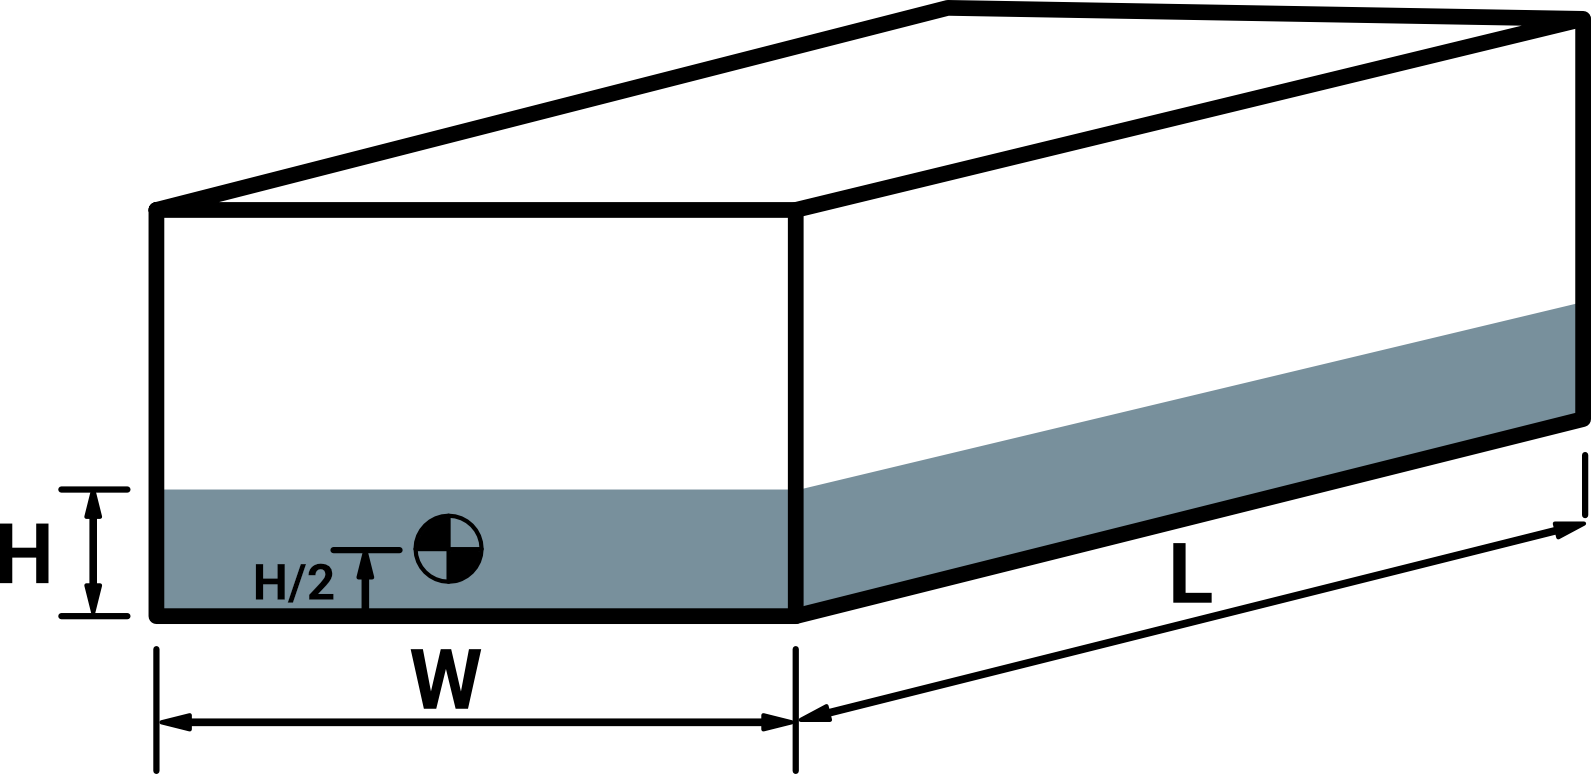
\includegraphics[width=0.5\textwidth]{fig/jad_payload_cgz_min}
	\caption{Minimum payload \gls{cgz} height}
	\label{figure:minimum-payload-cgz-height}
\end{figure}
%----------------------------------------------
%      FIGURE
%----------------------------------------------

The calculations of the minimum \gls{cgz} for each vehicle unit are summarised in Table~\ref{table:minimum-cgz-for-the-payload}.

%----------------------------------------------
%      TABLE - UPDATED TO NEW RANGES
%----------------------------------------------
\begin{table}[H]
	\centering\footnotesize
	\begin{threeparttable}

		\begin{tabulary}{\textwidth}{lCCCCCCc}
			\toprule
			\textbf{Combination} & \textbf{Width (m)} & \textbf{Length (m)} & \textbf{Payload density (kg/m\ssth)} & \textbf{Payload mass (kg)} & \textbf{H/2 (mm)} & \textbf{Deck height (mm)} & \textbf{Min. \gls{cgz}\tnote{1} (mm)} \\
			\midrule
            Rigid truck & 2.600   & 6.289 & 8050  & 14140 & 54 & 1068 & 1122\\
			Quad semi-trailer & 2.600   & 14.900 & 8050  & 32300 & 52 & 1528 & 1580\\
			Tridem interlink leader & 2.600   & 7.940 & 8050  & 24615 & 74 & 1593 & 1667\\
			Tridem interlink follower & 2.600   & 7.940 & 8050  & 24615 & 74 & 1593 &  1667\\
			Tridem semi-trailer & 2.600   & 12.456 & 8050  & 37000 & 71 & 1300 &  1371\\
			\bottomrule
		\end{tabulary}

		\caption{Minimum \gls{cgz} for the payload}
		\label{table:minimum-cgz-for-the-payload}

		\begin{tablenotes}
		\item[1] Measured from the ground
		\end{tablenotes}

	\end{threeparttable}
\end{table}
%----------------------------------------------
%      TABLE
%----------------------------------------------

The maximum payload \gls{cgz} height was determined from the geometrical location of the centre of gravity for a trapezoid with sides sloped at 20\degree{} according to Equation~\ref{equation:maximum-cgz-height}. This represents the payload distribution of a side-tipper filled to the top with payload which is typical for the transport of payloads with low densities.

%----------------------------------------------
%      EQUATION
%----------------------------------------------
\begin{align}
	\label{equation:maximum-cgz-height}
	y = h  \left ( 1 - \frac{1}{3} \times \frac{(b+2a)}{(b+a)} \right )
\end{align}

Where: $y$, $h$, $b$, and $a$ are the dimensions of the trapezoid as illustrated in Figure~\ref{figure:maximum-payload-cgz-height}.
%----------------------------------------------
%      EQUATION
%----------------------------------------------

%----------------------------------------------
%      FIGURE
%----------------------------------------------
\begin{figure}[H]
	\centering
	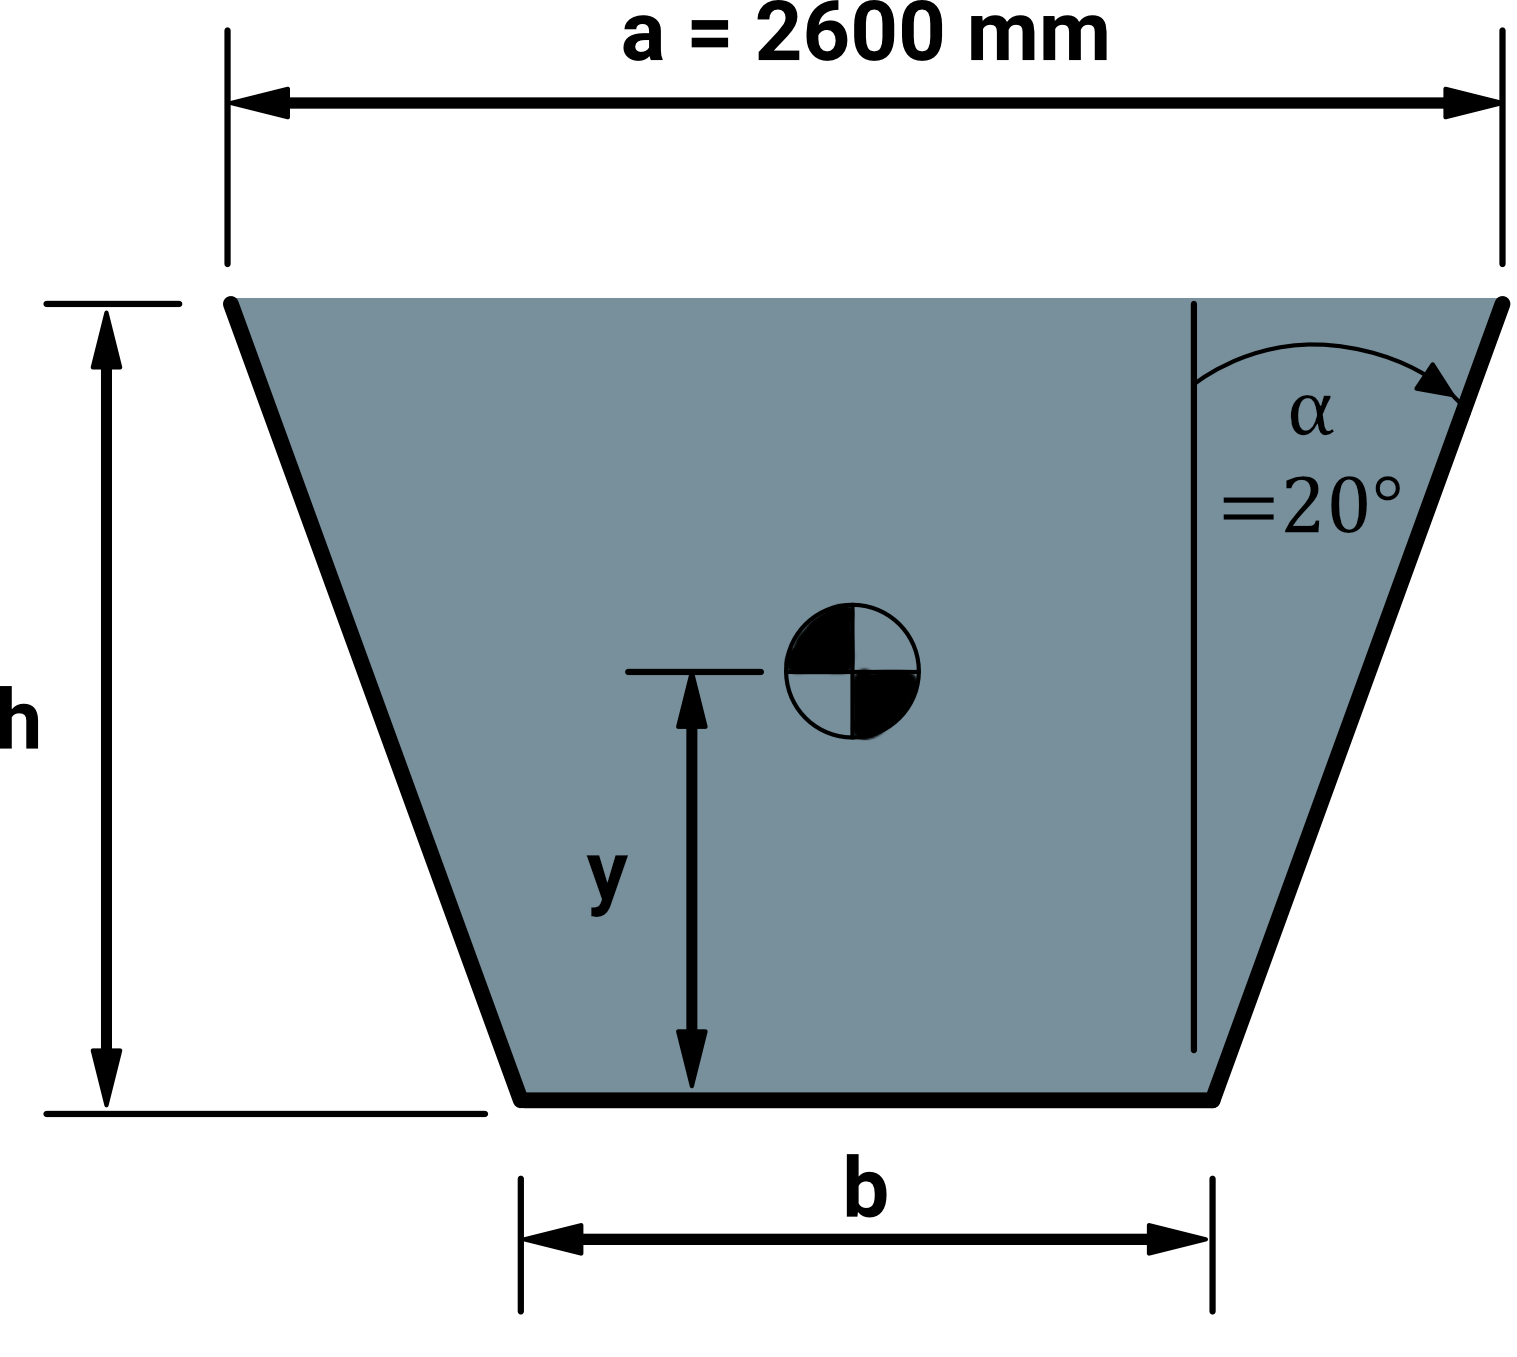
\includegraphics[width=0.5\textwidth]{fig/jad_payload_cgz_max}
	\caption{Maximum payload \gls{cgz} height}
	\label{figure:maximum-payload-cgz-height}
\end{figure}
%----------------------------------------------
%      FIGURE
%----------------------------------------------

The calculations for the maximum \gls{cgz} above ground are summarised in Table~\ref{table:payload-estimate-of-maximum-cgz-above-ground}.

%----------------------------------------------
%      TABLE - UPDATED TO NEW RANGES
%----------------------------------------------
\begin{table}[H]
	\centering\footnotesize
	\begin{threeparttable}

		\begin{tabulary}{\textwidth}{lccccC}
			\toprule
			\textbf{Combination} & \textbf{h (mm)} & \textbf{b (mm)} & \textbf{y (mm)} & \textbf{Deck height (mm)\tnote{1}} & \textbf{Max. \gls{cgz} (mm)\tnote{1}} \\

			\midrule
            Rigid truck & 3046  & 383   & 1900  & 1068  & 2968 \\
			Quad semi-trailer & 2272  & 946   & 1313  & 1528  & 2841 \\
			Tridem interlink leader & 1605  & 1432  & 880   & 1593  & 2473 \\
			Tridem interlink follower & 1605  & 383   & 880   & 1593  & 2473 \\
			Tridem semi-trailer & 2814  & 552   & 1712  & 1300  & 3012 \\
			\bottomrule
		\end{tabulary}

		\caption{Calculation of the maximum \gls{cgz} above ground}
		\label{table:payload-estimate-of-maximum-cgz-above-ground}

		\begin{tablenotes}
			\item[1] Measured from the ground
		\end{tablenotes}

	\end{threeparttable}
\end{table}
%----------------------------------------------
%      TABLE
%----------------------------------------------

%      SUBSECTION
%----------------------------------------------
\subsection{Payload Roll Moment of Inertia}\label{section:pr-roll-radius-of-gyration-payload}

The payload roll moment of inertia was assumed to vary according to the roll radius of gyration by an additional 5\% variation in comparison to the trailer vehicle units (see Section~\ref{section:pr-roll-moment-of-inertia-trailer-vehicle-units})  to account for the fact that payload geometry has additional scope to vary.

\begin{itemize}
\item \textbf{Payload \gls{rx} variation:} +/-50\%.
\end{itemize}

%      SUBSECTION
%----------------------------------------------
\subsection{Payload Pitch and Yaw Moment of Inertia}\label{section:pr-pitch-yaw-radius-of-gyration-payload}

There is additional scope for the pitch and yaw moment of inertia to vary relative to the roll moment of inertia. Thus, the payload pitch and yaw moment of inertia was assumed to vary according to the pitch and yaw radius of gyration by an additional 10\% in comparison to the trailer vehicle units unit (see Section~\ref{section:pr-pitch-yaw-radius-of-gyration-vehicle-units}) to account for the fact that payload has additional scope to vary.

\begin{itemize}
\item \textbf{Payload \gls{ry} and \gls{rz} variation:} +/-60\%.
\end{itemize}

%==============================================
%      SECTION
%==============================================
\section{Suspension Parameter Limits}\label{section:pr-suspension-parameter-limits}

The suspension parameter limits are often difficult to acquire from \glspl{oem}. Local distributors require permission from overseas design offices to release the proprietary information. Additionally, non-disclosures need to be signed when receiving technical information which can delay the data acquisition process.

To develop the evaluated ranges of the suspension parameter limits, existing literature was consulted for methods of estimating parameters and publicly available \gls{oem} datasheets were used to determine representative design parameters.

For some suspension parameters, data collected from \gls{pbs} assessments completed by \gls{wits} was used to investigate reasonable ranges. This data is protected by non-disclosure agreements and cannot be publicly disclosed in this dissertation. However variations in parameter values is presented relative to the baseline models.

A collection of measured vehicle design parameters is contained in studies such as those conducted by Fancher et al. \cite{Fancher1986} , \cite{Fancher1987}, Ervin et al. \cite{Ervin1986} and Harwood et al. \cite{Harwood2003}. These studies were conducted in the USA and Canada and may not be representative of the South African heavy vehicle fleet. These sources were used due to the lack of similar studies related to South African vehicles.

\subsection{Unsprung Mass}\label{section:pr-axle-unsprung-mass}

\textbf{Prime mover:} The unsprung masses recorded by Fancher et al. \cite{Fancher1986} for steer and drive axles as shown in Table~\ref{table:measured-unsprung-masses-fancher-et-al} are significantly lower than those generally observed in more modern prime movers. Therefore these were conservatively used as the minimum. The maximum steer and drive axle unsprung masses were determined from South African \gls{pbs} assessments and are included in Table \ref{table:pr-axle-unsprung-mass}.

%----------------------------------------------
%      TABLE
%----------------------------------------------
\begin{table}[H]
	\centering\footnotesize
	\begin{threeparttable}

		\begin{tabulary}{\textwidth}{lcc}
			\toprule
			\textbf{Axle type} & \textbf{Minimum (kg)} & \textbf{Maximum (kg)} \\
			\midrule
			Steer & \multicolumn{2}{c}{544}\\
			Drive & 1043  & 1134 \\
			Trailer & \multicolumn{2}{c}{798}\\
			\bottomrule
		\end{tabulary}

		\caption{Measured unsprung mass for steer, drive and trailer axles - Fancher et al. \cite{Fancher1986}}
		\label{table:measured-unsprung-masses-fancher-et-al}

		%\begin{tablenotes}
		%\item[1] %\tnote{1}
		%\end{tablenotes}

	\end{threeparttable}
\end{table}
%----------------------------------------------
%      TABLE
%----------------------------------------------

The range of unsprung masses for the trailer axles was determined from a collection of \gls{oem} data,  weights of generic suspension components collected from previous on-site measurements and South African \gls{pbs} assessments. 

To determine the minimum unsprung mass, data from the BPW axle catalogue was consolidated (see Tables~\ref{table:bpw-rigid-axles-with-300-mm-drum-brake}~to~\ref{table:bpw-rigid-axles-with-430-mm-disc-brake} included in Appendix \ref{section:bpw-rigid-axles-catalogue}). 

The minimum axle unpsrung mass was determined by combining the lightest BPW axle was with aluminium rims. The results of these calculations are summarised in Tables~\ref{table:unsprung-axle-mass-trailer-445-65-R22.5-singles-min}~to~\ref{table:unsprung-axle-mass-trailer-285-70-R19.5-duals-min}. 

The maximum trailer unsprung mass for each axle was determined from South African \gls{pbs} assessments since these were found to be heavier than the combination of the heaviest BPW axle with steel rims. The range of evaluated unsprung masses is summarised in Table~\ref{table:pr-axle-unsprung-mass}.

%----------------------------------------------
%      TABLE
%----------------------------------------------
\begin{table}[H]
	\centering\footnotesize
	\begin{threeparttable}

		\begin{tabulary}{\textwidth}{rrrrc}
			\toprule
			\multicolumn{1}{l}{\textbf{Component}} & \multicolumn{1}{c}{\textbf{Description}} & \multicolumn{1}{c}{\textbf{Quantity}} & \multicolumn{1}{c}{\textbf{Unit mass (kg)}} & \textbf{Total mass (kg)} \\
			\midrule
			\multicolumn{1}{l}{Tyre} & \multicolumn{1}{c}{445/65 R22.5} & \multicolumn{1}{c}{2} & \multicolumn{1}{c}{103.0} & 206.0 \\
			\multicolumn{1}{l}{Rim} & \multicolumn{1}{c}{Aluminium - 13"} & \multicolumn{1}{c}{2} & \multicolumn{1}{c}{26.5} & 53.0 \\
			\multicolumn{1}{l}{Axle} & \multicolumn{1}{c}{SKHSF 9010 (singles)} & \multicolumn{1}{c}{1} & \multicolumn{1}{c}{265.0} & 265.0 \\
			\multicolumn{1}{l}{Spring} & \multicolumn{1}{c}{Generic} & \multicolumn{1}{c}{2} & \multicolumn{1}{c}{5.6} & 11.2 \\
			\multicolumn{1}{l}{Damper} & \multicolumn{1}{c}{Generic} & \multicolumn{1}{c}{2} & \multicolumn{1}{c}{5.0} & 10.0 \\
            \midrule
			\multicolumn{4}{r}{\textbf{Total}} & 545.2 \\
			\bottomrule
		\end{tabulary}

		\caption{Minimum unsprung mass for a trailer axle with 445/65 R22.5 singles}
		\label{table:unsprung-axle-mass-trailer-445-65-R22.5-singles-min}

		%\begin{tablenotes}
		%\item[1] %\tnote{1}
		%\end{tablenotes}

	\end{threeparttable}
\end{table}
%----------------------------------------------
%      TABLE
%----------------------------------------------

%----------------------------------------------
%      TABLE
%----------------------------------------------
\begin{table}[H]
	\centering\footnotesize
	\begin{threeparttable}

		\begin{tabulary}{\textwidth}{rrrrc}
			\toprule
			\multicolumn{1}{l}{\textbf{Component}} & \multicolumn{1}{c}{\textbf{Description}} & \multicolumn{1}{c}{\textbf{Quantity}} & \multicolumn{1}{c}{\textbf{Unit mass (kg)}} & \textbf{Total mass (kg)} \\
			\midrule
			\multicolumn{1}{l}{Tyre} & \multicolumn{1}{c}{315/80 R22.5} & \multicolumn{1}{c}{4} & \multicolumn{1}{c}{68.7} & 274.8 \\
			\multicolumn{1}{l}{Rim} & \multicolumn{1}{c}{Aluminium - 9"} & \multicolumn{1}{c}{4} & \multicolumn{1}{c}{22.6} & 90.6 \\
			\multicolumn{1}{l}{Axle} & \multicolumn{1}{c}{SKHZF 9010 (duals)} & \multicolumn{1}{c}{1} & \multicolumn{1}{c}{280.0} & 280.0 \\
			\multicolumn{1}{l}{Spring} & \multicolumn{1}{c}{Generic} & \multicolumn{1}{c}{2} & \multicolumn{1}{c}{5.6} & 11.2 \\
			\multicolumn{1}{l}{Damper} & \multicolumn{1}{c}{Generic} & \multicolumn{1}{c}{2} & \multicolumn{1}{c}{5.0} & 10.0 \\
            \midrule
			\multicolumn{4}{r}{\textbf{Total}} & 666.5 \\
			\bottomrule
		\end{tabulary}

		\caption{Minimum unsprung mass for a trailer axle with 315/80 R22.5 duals}
		\label{table:unsprung-axle-mass-trailer-315-80-R22.5-duals-min}

		%\begin{tablenotes}
		%\item[1] %\tnote{1}
		%\end{tablenotes}

	\end{threeparttable}
\end{table}
%----------------------------------------------
%      TABLE
%----------------------------------------------

%----------------------------------------------
%      TABLE
%----------------------------------------------
\begin{table}[H]
	\centering\footnotesize
	\begin{threeparttable}

		\begin{tabulary}{\textwidth}{rrrrc}
			\toprule
			\multicolumn{1}{l}{\textbf{Component}} & \multicolumn{1}{c}{\textbf{Description}} & \multicolumn{1}{c}{\textbf{Quantity}} & \multicolumn{1}{c}{\textbf{Unit mass (kg)}} & \textbf{Total mass (kg)} \\
			\midrule
			\multicolumn{1}{l}{Tyre} & \multicolumn{1}{c}{285/70 R19.5} & \multicolumn{1}{c}{4} & \multicolumn{1}{c}{41.0} & 164.0 \\
			\multicolumn{1}{l}{Rim} & \multicolumn{1}{c}{Aluminium - 7.5"} & \multicolumn{1}{c}{4} & \multicolumn{1}{c}{18.7} & 74.7 \\
			\multicolumn{1}{l}{Axle} & \multicolumn{1}{c}{SKHZF 9008 (duals)} & \multicolumn{1}{c}{1} & \multicolumn{1}{c}{270.0} & 270.0 \\
			\multicolumn{1}{l}{Spring} & \multicolumn{1}{c}{Generic} & \multicolumn{1}{c}{2} & \multicolumn{1}{c}{5.6} & 11.2 \\
			\multicolumn{1}{l}{Damper} & \multicolumn{1}{c}{Generic} & \multicolumn{1}{c}{2} & \multicolumn{1}{c}{5.0} & 10.0 \\
            \midrule
			\multicolumn{4}{r}{\textbf{Total}} & 529.8 \\

			\bottomrule
		\end{tabulary}

		\caption{Minimum unsprung mass for a trailer axle with 285/70 R19.5 duals}
		\label{table:unsprung-axle-mass-trailer-285-70-R19.5-duals-min}

		%\begin{tablenotes}
		%\item[1] %\tnote{1}
		%\end{tablenotes}

	\end{threeparttable}
\end{table}
%----------------------------------------------
%      TABLE
%----------------------------------------------

%----------------------------------------------
%      TABLE - UPDATED TO NEW RANGES
%----------------------------------------------
\begin{table}[H]
	\centering\footnotesize
	\begin{threeparttable}

		\begin{tabulary}{\textwidth}{lccc}
			\toprule
			\textbf{Axle} & \textbf{Baseline (kg)} & \textbf{Min (kg)} & \textbf{Max (kg)} \\
			\midrule
			Steer & 750   & 544   & 800 \\
			Drive & 1300  & 1043   & 1350 \\
			Trailer (445/65 R22.5 - singles) & 760   & 545   & 800 \\
			Trailer (315/80 R22.5 - duals) & 900   & 667   & 1000 \\
			Trailer (285/70 R19.5 - duals) & 757   & 530   & 850 \\
			\bottomrule
		\end{tabulary}

		\caption{Parameter range - axle unsprung mass}
		\label{table:pr-axle-unsprung-mass}

		%\begin{tablenotes}
		%\item[1] %\tnote{1}
		%\end{tablenotes}

	\end{threeparttable}
\end{table}
%----------------------------------------------
%      TABLE
%----------------------------------------------

\subsection{Axle Roll and Yaw Moment of Inertia}\label{section:pr-axle-roll-yaw-inertia}
According to Winkler et al. \cite{Winkler2011}, the axle roll and yaw moment of inertia (\gls{ixx}/\gls{izz}) for steer, drive and trailer axles can be estimated with the range of radii of gyration provided in Table~\ref{table:estimated roll/yaw radius of gyrations for axles}. The axle \gls{rx} and \gls{rz} are approximately equal and are thus treated as a single \gls{vdp}.

%----------------------------------------------
%      TABLE
%----------------------------------------------
\begin{table}[H]
	\centering\footnotesize
	\begin{threeparttable}

		\begin{tabulary}{\textwidth}{lcc}
			\toprule
			\textbf{Axle type} & \textbf{Min. \gls{rx}/\gls{rz} (mm)} & \textbf{Max. \gls{rx}/\gls{rz} (mm)} \\
			\midrule
			Steer & 840 & 910\\
			Drive & 690 & 740\\
			Trailer & 790 & 860 \\
			\bottomrule
		\end{tabulary}

		\caption{Estimation range for axle \gls{rx}/\gls{rz} \cite{Winkler2011}}
		\label{table:estimated roll/yaw radius of gyrations for axles}

		%\begin{tablenotes}
		%\item[1] %\tnote{1}
		%\end{tablenotes}

	\end{threeparttable}
\end{table}
%----------------------------------------------
%      TABLE
%----------------------------------------------

The minimum and maximum axle roll and yaw inertias were determined using the baseline axle unsprung mass with the minimum and maximum axle roll and yaw radii of gyrations from Winkler et al. (see Table~\ref{table:estimated roll/yaw radius of gyrations for axles}).

The resulting range of axle roll and yaw inertia for each baseline axle is provided in Table~\ref{table:parameter-range-axle-roll-and-yaw-inertia}.

%----------------------------------------------
%      TABLE - UPDATED TO NEW RANGES
%----------------------------------------------
\begin{table}[H]
	\centering\footnotesize
	\begin{threeparttable}

		\begin{tabulary}{\textwidth}{lccc}
			\toprule
			\textbf{Axle} & \textbf{Baseline (kg.m\sstw)} & \textbf{Min. (kg.m\sstw)} & \textbf{Max. (kg.m\sstw)} \\
			\midrule
             Steer & 529   & 529   & 621 \\
             Drive & 619   & 619   & 712 \\
             Trailer (445/65 R22.5 singles)  & 474   & 474   & 562 \\
             Trailer (315/80 R22.5 duals) & 562   & 562   & 666 \\
             Trailer (285/70R22.5 duals) & 472   & 472   & 560 \\
			\bottomrule
		\end{tabulary}

		\caption{Parameter range - axle roll and yaw moment of inertia}
		\label{table:parameter-range-axle-roll-and-yaw-inertia}

		%\begin{tablenotes}
		%\item[1] %\tnote{1}
		%\end{tablenotes}

	\end{threeparttable}
\end{table}
%----------------------------------------------
%      TABLE
%----------------------------------------------

%      SUBSECTION
%----------------------------------------------
\subsection{Axle Spin Moment of Inertia}\label{section:pr-axle-spin-moment-of-inertia}

The spin inertia of the rotating components of the axle is generally quite small. A value of 2~kg.m\sstw{} was derived by de Saxe \cite{DeSaxe2012} from measured data published by Winkler et al. \cite{Winkler1995} which was considered the minimum value. The \trucksim{} 2018 database includes spin inertias of up to 20~kg.m\sstw{} (\textit{18t Trailer, Dual Wheels}) which was deemed reasonable as the maximum value for the spin inertia of the rotating axle components.

%      SUBSECTION
%----------------------------------------------
\subsection{Damper Dynamic Response}\label{section:pr-axle-damper}

Linear damping models in the \trucksim{} 2018 database range from 2.5~kN-s/m to 50~kN-s/m. Due to the complex nature of comparing the damping characteristics of non-linear damping, the effectiveness of which is dependent on the range of operation, the baseline damping was linearised and the damping was varied from 2.5~to~50~kN-s/m.

%      SUBSECTION
%----------------------------------------------
\subsection{Roll Steer Coefficient}\label{section:pr-roll-steer}

\gls{rollsteer} is the tendency for a non-steered rigid axle to exhibit some level of steering as an axle rolls relative to the vehicles sprung mass such as when travelling over a disturbance or when performing certain turning manoeuvres. An exaggerated illustration of this effect is shown in Figure~\ref{figure:Illustration-of-the-roll-steer-effect-on-a-rigid-axle}.

%----------------------------------------------
%      FIGURE
%----------------------------------------------
\begin{figure}[!htbp]
	\centering
	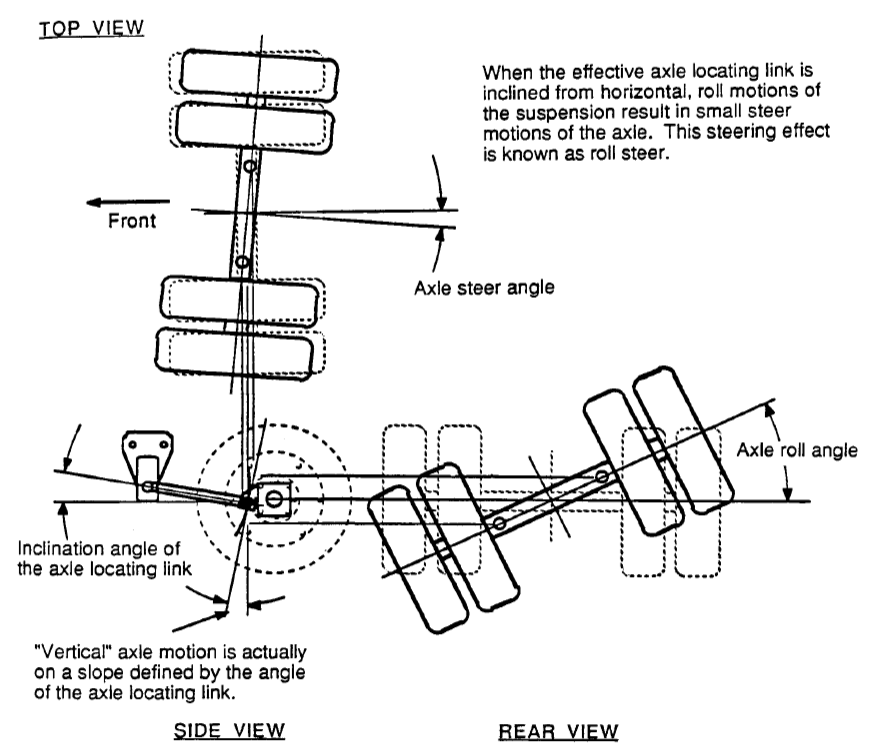
\includegraphics[width=1\textwidth]{fig/fancher-1986_roll-steer-illustration}
	\caption{Illustration of the roll steer effect on a rigid axle \cite{Fancher1986}}
	\label{figure:Illustration-of-the-roll-steer-effect-on-a-rigid-axle}
\end{figure}
%----------------------------------------------
%      FIGURE
%----------------------------------------------

Studies conducted by both Fancher et al. \cite{Fancher1986} and Harwood et al. \cite{Harwood2003} have resulted in a collection of measured roll steer coefficients. A comparison of the data from these sources is included in Table~\ref{table:comparison-of-roll-steer-coefficients}\footnote{The data published is according to the ISO coordinate system with the Z-axis (vertical) positive down and steering to the right as positive. The \trucksim{} coordinate system makes use of the SAE up coordinate system with the Z-axis positive up and steering to the left as positive. The data in this table has been converted from the published values to the SAE up coordinate system}.

%----------------------------------------------
%      TABLE
%----------------------------------------------
\begin{table}[H]
	\centering\footnotesize
	\begin{threeparttable}

		\begin{tabulary}{\textwidth}{lcccc}
			\toprule
			& \multicolumn{2}{c}{\textbf{Fancher et al. \cite{Fancher1986}}} & \multicolumn{2}{c}{\textbf{Harwood et al. \cite{Harwood2003}}} \\\cline{2-5}
			\textbf{Suspension type} & \multicolumn{1}{l}{\textbf{Min.}} & \multicolumn{1}{l}{\textbf{Max.}} & \multicolumn{1}{l}{\textbf{Min.}} & \multicolumn{1}{l}{\textbf{Max.}} \\
			\midrule
			Air suspension & -0.01 & -0.225 & -0.01 & -0.23 \\
			Single-axle leaf spring & 0     & -0.08 & 0     & -0.07 \\
			Steer axle & 0     & -0.2  &   -    & - \\
			Walking beam & -0.175 & -0.21 & -0.16 & -0.21 \\
			4-spring suspensions & 0.04  & -0.22 & -0.23 & 0.04 \\
			\bottomrule
		\end{tabulary}

		\caption{Measured roll steer coefficients from published data}
		\label{table:comparison-of-roll-steer-coefficients}

		%\begin{tablenotes}
		%\item[1] %\tnote{1}
		%\end{tablenotes}

	\end{threeparttable}
\end{table}
%----------------------------------------------
%      TABLE
%----------------------------------------------

The minimum and maximum values for the roll steer coefficient from Table~\ref{table:comparison-of-roll-steer-coefficients} were chosen to evaluate the broadest range of roll steer on each of the axles. The resulting range of values evaluated is summarised in Table~\ref{table:parameter-range-roll-steer-coefficients}.

%----------------------------------------------
%      TABLE - UPDATED TO NEW RANGES
%----------------------------------------------
\begin{table}[H]
	\centering\footnotesize
	\begin{threeparttable}

		\begin{tabulary}{\textwidth}{lccc}
			\toprule
			\textbf{Axle} & \textbf{Baseline (\degree{}/\degree{})} & \textbf{Min. (\degree{}/\degree{})} & \textbf{Max. (\degree{}/\degree{})} \\
			\midrule
			Steer & -0.087 & 0     & -0.2 \\
			Drive & 0     & 0.04  & -0.23 \\
			Trailer (singles) & -0.035 & 0.04  & -0.23 \\
			Trailer (duals) & -0.156 & 0.04  & -0.23 \\
			\bottomrule
		\end{tabulary}

		\caption{Parameter range - roll steer coefficients}
		\label{table:parameter-range-roll-steer-coefficients}

		%\begin{tablenotes}
		%\item[1] %\tnote{1}
		%\end{tablenotes}

	\end{threeparttable}
\end{table}
%----------------------------------------------
%      TABLE
%----------------------------------------------

%      SUBSECTION
%----------------------------------------------
\subsection{Axle Track}\label{section:pr-axle-track}

At a Smart Truck Review Panel meeting held in 2017, it was passed that the overall axle track width on a \gls{pbs} vehicle may exceed the legal limit of 2600~mm up to 2650~mm (zero tolerance and including tyre bulge). This is to allow increased axle track and thus improved stability for \gls{pbs} combinations.

It would not be practical for prime mover manufacturers to modify their designs to consider the new relaxations since they would not be able to be used in conjunction with a legal vehicle. Thus, a maximum overall width of 2600~mm was evaluated for the steer and drive axle. To account for new trailer designs that may take advantage of this new relaxation, the maximum axle track was found using a maximum overall axle width of 2650~mm with the minimum tyre spacing as specified by Michelin in their tyre data book \cite{Michelin}.

\textbf{Maximum axle track conditions:}

\begin{enumerate}
	\item Overall width of 2600~mm for steer and drive axle and 2650~mm for trailer axles.
	\item The dual tyres were arranged to have the minimum spacing as recommended by Michelin \cite{Michelin}.
\end{enumerate}

\textbf{Minimum axle track conditions:}

No regulations were defined for minimum axle track width. A catalogue of rigid axles supplied by BPW (see Appendix~\ref{section:bpw-rigid-axles-catalogue}) \cite{BPW2010} was consulted to determine the minimum axle tracks available to avoid evaluation of unrepresentative narrow axle tracks. Only axles in the 9000 kg + rated load category were considered.

A selection of the BPW axles illustrating the variability of their axle tracks is provided in Table~\ref{table:bpw-axle-tracks}.

%----------------------------------------------
%      TABLE
%----------------------------------------------
\begin{table}[H]
	\centering\footnotesize
	\begin{threeparttable}

		\begin{tabulary}{\textwidth}{lccccc}
			\toprule
			\textbf{Axle Model} & \textbf{Tyre arrangement} & \textbf{Rim} & \textbf{Rated load (kg)} & \textbf{Min. (mm)} & \textbf{Max. (mm)} \\
			\midrule
			NHZF  & Duals & 19.5" & 9000  & 1830  & 1995 \\
			SHZF  & Duals & 22.5" & 9000-12000 & 1820  & 1880 \\
			SKHSF & Singles & 22.5" & 9000  & 2000  & 2140 \\
			\bottomrule
		\end{tabulary}

		%\begin{tablenotes}
		%\item[1] %\tnote{1}
		%\end{tablenotes}
        
        \caption{BPW axle tracks}
		\label{table:bpw-axle-tracks}

	\end{threeparttable}
\end{table}
%----------------------------------------------
%      TABLE
%----------------------------------------------

A limiting factor was the baseline spring and damper track, it was ensured that the edge of the tyres did not move past the spring or damper centre. In all cases, the minimum tracks from the BPW catalogue were suitable and did not cause interference with the spring or damper track.

In addition to the BPW axles, data collected from Fancher et al. \cite{Fancher1986} was used to consider alternative \glspl{oem} as well as ranges of steer axle track widths. A summary of the representative track widths is included in Table~\ref{table:measured-axle-track-widths-from-fancher-et-al}. The data from Fancher et al. is for American based vehicles with tractor widths of 96" (approx. 2439~mm) and trailer widths of 102" (approx. 2591~mm) which closely approximate the widths of local heavy vehicles. Thus, the axle track widths were deemed to be representative for vehicles operating within South Africa.

%----------------------------------------------
%      TABLE
%----------------------------------------------
\begin{table}[H]
	\centering\footnotesize
	\begin{threeparttable}

		\begin{tabulary}{\textwidth}{lcc}
			\toprule
			\textbf{Axle} & \textbf{Min. (mm)} & \textbf{Max. (mm)} \\
			\midrule
			Steer (96" cab width) & 1956  & 2057 \\
			Drive (96" cab width) & 1803  & 1829 \\
			Trailer (102" trailer width) & 1956  & 1981 \\
			\bottomrule
		\end{tabulary}

		\caption{Measured axle track widths from Fancher et al. \cite{Fancher1986}}
		\label{table:measured-axle-track-widths-from-fancher-et-al}

		%\begin{tablenotes}
		%\item[1] %\tnote{1}
		%\end{tablenotes}

	\end{threeparttable}
\end{table}
%----------------------------------------------
%      TABLE
%----------------------------------------------

Considering the worst-case minimum from either the BPW data book or Fancher et al. \cite{Fancher1986}, the range of axle tracks evaluated for each axle is included in Table~\ref{table:parameter-range-axle-track}.

%----------------------------------------------
%      TABLE - UPDATED TO NEW RANGES
%----------------------------------------------
\begin{table}[H]
	\centering\footnotesize
	\begin{threeparttable}

		\begin{tabulary}{\textwidth}{lccc}
			\toprule
             \textbf{Axle} & \textbf{Baseline (mm)} & \textbf{Min. (mm)} & \textbf{Max. (mm)} \\
			\midrule
             Steer & 2109  & 1950  & 2282 \\
             Drive & 1837  & 1800  & 1932 \\
             Trailer (445/65 R22.5 singles)  & 2140  & 2000  & 2178 \\
             Trailer (315/80 R22.5 duals) & 1920  & 1820  & 1982 \\
             Trailer (285/70R22.5 duals) & 2040  & 1830  & 2042 \\
			\bottomrule
		\end{tabulary}

		\caption{Parameter range - axle track width}
		\label{table:parameter-range-axle-track}

		%\begin{tablenotes}
		%\item[1] %\tnote{1}
		%\end{tablenotes}

	\end{threeparttable}
\end{table}
%----------------------------------------------
%      TABLE
%----------------------------------------------

\subsection{Spring and Damper Track}\label{section:spring and damper track}

The BPW axle catalogues \cite{BPW2010} (see Appendix~\ref{section:bpw-rigid-axles-catalogue}) were also used to develop the range of spring tracks. 

The minimum spring track from the BPW catalogues was chosen as the minimum for the trailer, drive and steer axles. The maximum BPW spring track was used as the maximum for the trailer axles. The maximum steer and drive axle tracks was limited by the baseline suspension geometry.

For all axles, it was assumed that the damper track could vary within the same range as the spring track. The resulting range of evaluated spring and damper tracks is summarised in Table~\ref{table:bpw-spring-and-damper-tracks}.

%----------------------------------------------
%      TABLE
%----------------------------------------------
\begin{table}[H]
	\centering\footnotesize
	\begin{threeparttable}

		\begin{tabulary}{\textwidth}{lccccc}
			\toprule
			\textbf{Axle} & \multicolumn{1}{l}{\textbf{Min. (mm)}} & \multicolumn{1}{l}{\textbf{Max. (mm)}} \\
			\midrule

			Steer & 780 & 1150 \\
			Drive & 670 & 1100 \\
			Trailer (single tyre) & 780 & 1500 \\
			Trailer (dual tyre) & 670 & 1200 \\
			\bottomrule
		\end{tabulary}

		%\begin{tablenotes}
		%\item[1] %\tnote{1}
		%\end{tablenotes}
        
        \caption{Parameter range - spring and damper track width}
		\label{table:bpw-spring-and-damper-tracks}

	\end{threeparttable}
\end{table}
%----------------------------------------------
%      TABLE
%----------------------------------------------


%      SUBSECTION
%----------------------------------------------
\subsection{Spring Vertical Stiffness}\label{section:pr-spring-stiffness}

The range of spring vertical stiffness values were determined from spring data collected from PBS assessments conducted by Wits University\footnote{\gls{oem} data protected by non-disclosure agreements and hence anonymised in this dissertation}.

The dynamic spring response for airbags is dependent on the vertical load. To compare the dynamic spring response, the response was linearly interpolated to a vertical load of 25000~N.

The results contained in Table \ref{table:comparison-of-dynamic-response-of-airbag-springs} indicate that there are significant variations (up to 186\%) in the spring stiffness between the different airbags at the static vertical load of 25000~N. It was assumed that any of the springs could be fitted to any of the axles to evaluate the full range of possibilities.

%----------------------------------------------
%      TABLE
%----------------------------------------------
\begin{table}[H]
	\centering\footnotesize
	\begin{threeparttable}
    
    	\caption{Comparison of the stiffness of airbag springs at 25000~N}
		\label{table:comparison-of-dynamic-response-of-airbag-springs}

		\begin{tabulary}{\textwidth}{lCCC}
			\toprule
			\textbf{Airbag type} & \textbf{Interpolated stiffness at 25000~N (N/mm)} & \textbf{Variation from drive axle baseline (\%)} & \textbf{Variation from trailer axle baseline (\%)} \\
			\midrule
			Trailer & 104   & 47\%  & 69\% \\
			Trailer & 205   & 92\%  & 137\% \\
			Drive & 94    & 42\%  & 62\% \\
			Steer & 157   & 71\%  & 105\% \\
			Drive & 115   & 52\%  & 77\% \\
			Drive & 155   & 70\%  & 103\% \\
			Drive & 270   & 121\% & 180\% \\
			Drive & 130   & 59\%  & 87\% \\
			Drive & 150   & 67\%  & 100\% \\
			Drive & 280   & 126\% & 186\% \\
			Drive & 100   & 45\%  & 67\% \\
			Drive & 122   & 55\%  & 82\% \\
			Drive & 222   & 100\% & 148\% \\
			Drive & 140   & 63\%  & 93\% \\
			Drive & 280   & 126\% & 186\% \\
			Trailer & 150   & 67\%  & 100\% \\
			Trailer & 151   & 68\%  & 100\% \\
			\bottomrule
		\end{tabulary}

		%\begin{tablenotes}
		%\item[1] %\tnote{1}
		%\end{tablenotes}

	\end{threeparttable}
\end{table}
%----------------------------------------------
%      TABLE
%----------------------------------------------

The baseline steer axles are fitted with a steel spring suspension. Sample steel spring stiffness values are provided in the \trucksim{} 2018 database that range from 200~N/mm to 350~N/mm. 350~N/mm was used as the maximum steel suspension stiffness. The minimum stiffness was evaluated as 185~N/mm according to the conservative spring stiffness used in the TERNZ \gls{srt} calculator \cite{TERNZTransportResearch} when a generic steer axle suspension is selected.

The resulting range of spring vertical stiffness values are provided in Table~\ref{table:parameter-range-spring-vertical-stiffness}. In the case of air springs, the baseline value is reported as 100\% of the baseline spring response, with the minimum and maximum variations scaled as a percentage of the baseline spring response.

%----------------------------------------------
%      TABLE
%----------------------------------------------
\begin{table}[H]
	\centering\footnotesize
	\begin{threeparttable}

		\begin{tabulary}{\textwidth}{lccc}
			\toprule
			\textbf{Axle} & \textbf{Baseline} & \textbf{Min.} & \textbf{Max.} \\
			\midrule
             Steer & 273 N/mm & 185 N/mm & 350 N/mm \\
             Drive & 100\% & 42\%  & 126\% \\
             Trailer & 100\% & 62\%  & 186\% \\
			\bottomrule
		\end{tabulary}

		\caption{Parameter range - spring vertical stiffness}
		\label{table:parameter-range-spring-vertical-stiffness}

		%\begin{tablenotes}
		%\item[1] %\tnote{1}
		%\end{tablenotes}

	\end{threeparttable}
\end{table}
%----------------------------------------------
%      TABLE
%----------------------------------------------

%      SUBSECTION
%----------------------------------------------
\subsection{Jounce and Rebound Stops}\label{section:pr-jounce-rebound-stops}

The jounce (upward movement) and rebound (downward movement) stops indicate the possible range of vertical movement for a suspension assembly as limited by mechanical constraints. Data collected from \gls{oem}s range from 45~mm to 110~mm up (jounce) and 50~mm to 120~mm down (rebound).

The \trucksim{} 2018 database includes jounce rebound stops of up to +250~mm / -250~mm. This is generally used as a conservative estimate in the case that an \gls{oem} does not supply sufficient information to determine jounce/rebound stops for the suspension. This was hence used as the worst case.

The lower end of the range was conservatively chosen from the \gls{oem} data with the upper end chosen from the \trucksim{} 2018 database due to the jounce and rebound stops rarely being supplied. 

To simplify the modelling, it was assumed that the jounce and rebound stops would be equal, resulting in the limits summarised in Table~\ref{table:parameter-jounce-and-rabound-stops} used for all baseline axles.

%----------------------------------------------
%      TABLE
%----------------------------------------------
\begin{table}[H]
	\centering\footnotesize
	\begin{threeparttable}

		\begin{tabulary}{\textwidth}{lccc}
			\toprule
			\textbf{Axle} & \textbf{Baseline} & \textbf{Min. (mm)} & \textbf{Max. (mm)} \\
			\midrule
			All & Varies & +45/-45 & +250/-250 \\
			\bottomrule
		\end{tabulary}

		\caption{Parameter range -  jounce and rebound stops}
		\label{table:parameter-jounce-and-rabound-stops}

		%\begin{tablenotes}
		%\item[1] %\tnote{1}
		%\end{tablenotes}

	\end{threeparttable}
\end{table}
%----------------------------------------------
%      TABLE
%----------------------------------------------

%      SUBSECTION
%----------------------------------------------
\subsection{Auxiliary Roll Stiffness}\label{section:pr-auxiliary-roll-stiffness}

To adhere to the \gls{pbs} requirement of a minimum \gls{srt} of 0.35~g, \gls{pbs} combinations are designed with higher auxiliary roll stiffness values to improve their rollover performance. Thus, the collected \gls{oem} data from South African \gls{pbs} assessments is skewed towards the suspensions with higher auxiliary roll stiffness. 

The \gls{oem} data is a good indicator of the upper end of auxiliary roll stiffness values while the data collected by Fu et al. \cite{Fu2002} from an analysis of several contemporary suspension designs is assumed to be a good indicator of the lower end of auxiliary roll stiffness values. 

A comparison of the ranges of auxiliary roll stiffness provided by \glspl{oem} is made with the data collected by Fu et al. in Table~\ref{table:comparison-of-auxiliary-roll-stiffness-ranges}. The resulting limits for auxiliary roll stiffness of each of the baseline axles is provided in Table \ref{table:parameter-range-auxiliary-roll-stiffness}.

%----------------------------------------------
%      TABLE - UPDATED TO NEW RANGES
%----------------------------------------------
\begin{table}[H]
	\centering\footnotesize
	\begin{threeparttable}

		\begin{tabulary}{\textwidth}{lCCCC}
			\toprule
			\textbf{Axle} & \makecell{\textbf{Min. (Nm/deg)} \\ \textbf{(OEM)}} & \makecell{\textbf{Max. (Nm/deg)} \\ \textbf{(OEM)}} & \makecell{\textbf{Min. (Nm/deg)} \\ \textbf{(Fu et al.)}} & \makecell{\textbf{Max. (Nm/deg)} \\ \textbf{(Fu et al.)}} \\
			\midrule
			Steer & 1850  & 5009  & 1070  & 1470 \\
			Drive & 7226  & 12689 & 790   & 2030 \\
			Trailer & 23736 & 35954 & 2260  & 13560 \\
			\bottomrule
		\end{tabulary}

		\caption{Comparison of auxiliary roll stiffness ranges from \glspl{oem} and Fu et al. \cite{Fu2002}}
		\label{table:comparison-of-auxiliary-roll-stiffness-ranges}

		%\begin{tablenotes}
		%\item[1] %\tnote{1}
		%\end{tablenotes}

	\end{threeparttable}
\end{table}
%----------------------------------------------
%      TABLE
%----------------------------------------------

%----------------------------------------------
%      TABLE - UPDATED TO NEW RANGES
%----------------------------------------------
\begin{table}[H]
	\centering\footnotesize
	\begin{threeparttable}

		\begin{tabulary}{\textwidth}{lccc}
			\toprule
			\textbf{Axle} & \textbf{Baseline} & \textbf{Min. (Nm/deg) (Fu et al.)} & \textbf{Max. (Nm/deg) (OEM)} \\
			\midrule
			Steer & 2950  & 1070  & 5009 \\
			Drive & 7487 & 790 & 12689 \\
			Trailer & 24700 & 2260  & 35954 \\
			\bottomrule
		\end{tabulary}

		\caption{Parameter range - auxiliary roll stiffness}
		\label{table:parameter-range-auxiliary-roll-stiffness}

		%\begin{tablenotes}
		%\item[1] %\tnote{1}
		%\end{tablenotes}

	\end{threeparttable}
\end{table}
%----------------------------------------------
%      TABLE
%----------------------------------------------

%      SUBSECTION
%----------------------------------------------
\subsection{Wheel and Axle Centre Height}\label{section:axle-centre-height}

The wheel centre height was assumed to vary from the laden height up to an increased height by half of the deflection between laden and unladen conditions (using the Michelin data book \cite{Michelin} for the unladen heights). These wheel centre height maximums are presented in Table~\ref{table:wheel-centre-height-variation-due-to-tyre-deflection}.

The height of the axle \gls{cg} is generally assumed equal to the wheel centre height since it is not supplied by the \glspl{oem} and detailed drawings (which tend to be proprietary) would be needed to determine the offset of the axle centre height relative to the wheel centre height.

The \trucksim{} 2018 database has a maximum axle centre offset relative to the wheel centre height of 60~mm (\textit{3t Drive, single wheels}). This was assumed to be the maximum offset above or below the wheel centre height resulting in the range of axle centre heights being evaluated as per Table \ref{table:parameter-range-wheel-and-axle-centre-height}.

%----------------------------------------------
%      TABLE - UPDATED TO NEW RANGES
%----------------------------------------------
\begin{table}[H]
	\centering\footnotesize
	\begin{threeparttable}

		\begin{tabulary}{\textwidth}{lcccC}
			\toprule
			\textbf{Tyre} & \makecell{\textbf{Laden radius} \\ \textbf{(mm)}} & \makecell{\textbf{Unladen radius} \\ \textbf{(mm)}} & \makecell{\textbf{Deflection} \\ \textbf{(mm)}} & \textbf{Max. wheel centre height (mm)}\\
			\midrule
            285/70 R19.5 & 413   & 456   & 42.50 & 434.3 \\
            315/80 R22.5 & 507   & 548   & 41.00 & 527.5 \\
            445/65 R22.5 & 534   & 587   & 53.00 & 560.5 \\
			\bottomrule
		\end{tabulary}

		\caption{Wheel centre height variation due to tyre deflection \cite{Michelin}}
		\label{table:wheel-centre-height-variation-due-to-tyre-deflection}

		%\begin{tablenotes}
		%\item[1] %\tnote{1}
		%\end{tablenotes}

	\end{threeparttable}
\end{table}
%----------------------------------------------
%      TABLE
%----------------------------------------------

%----------------------------------------------
%      TABLE - UPDATED TO NEW RANGES
%----------------------------------------------
\begin{table}[H]
	\centering\footnotesize
	\begin{threeparttable}

		\begin{tabulary}{\textwidth}{lccc}
			\toprule
			\textbf{Parameter} & \textbf{Baseline (mm)\tnote{1}} & \textbf{Min. (mm) } & \textbf{Max. (mm)}\\
			\midrule
            
            Wheel centre height (445/65 R22.5) & 534.0   & 534.0   & 560.5 \\
            Wheel centre height (315/80 R22.5) & 507.0  & 507.0   & 527.5 \\
            Wheel centre height (285/70 R19.5) & 413.0   & 413.0   & 434.3 \\          
            Axle centre height (445/65 R22.5) & 534.0   & 474.0   & 594.0 \\
            Axle centre height (315/80 R22.5) & 507.0   & 447.0   & 567.0 \\
            Axle centre height (285/70 R19.5) & 413.0   & 353.0  & 473.0 \\
            
			\bottomrule
		\end{tabulary}

		\caption{Parameter range - wheel and axle centre height}
		\label{table:parameter-range-wheel-and-axle-centre-height}

		\begin{tablenotes}
			\item[1] Height relative to the ground
		\end{tablenotes}

	\end{threeparttable}
\end{table}
%----------------------------------------------
%      TABLE
%----------------------------------------------

%      SUBSECTION
%----------------------------------------------
\subsection{Roll Centre Height}\label{section:pr-roll-centre-heights}

Winkler et al. \cite{Winkler2011} has documented a set of graphical methods for determining the roll centre based on the geometry of the suspension (see Figure~\ref{figure:estimate-of-roll-centre-heights-for-typical-suspension-configurations}). Using the graphical method for typical trailing arm suspensions, the maximum distance of the roll centre height from the centre of the axle is when the leaf spring makes an angle of 0\degree{} to the horizontal. Thus, the vertical distance from the centre of the lever arm to the centre of the axle will be a maximum when the thickness of the lever arm and cross-sectional height of the axle are at a maximum.

\begin{figure*}
	\centering
	\begin{subfigure}[t]{0.45\textwidth}
		\centering
		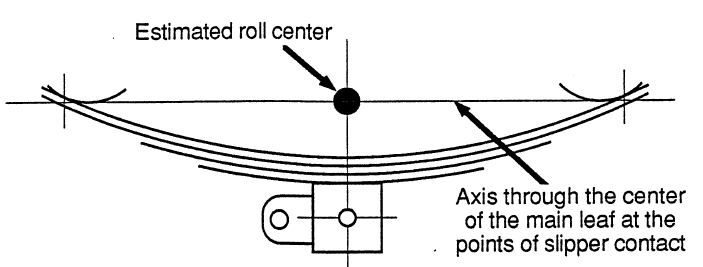
\includegraphics[height=1.2in]{fig/winkler-2011_roll-centre-estimation_typical-four-spring-suspensions}
		\caption{Typical four spring suspensions}
	\end{subfigure}%
	\hfill
	\begin{subfigure}[t]{0.45\textwidth}
		\centering
		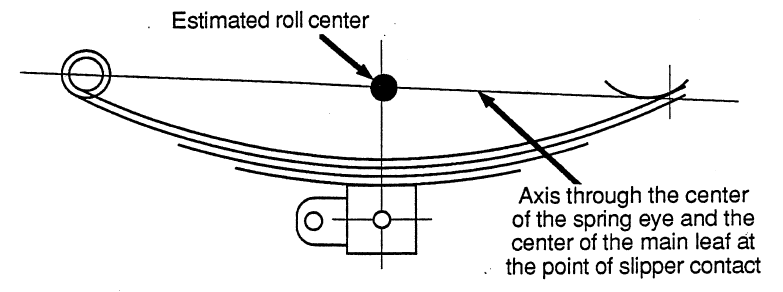
\includegraphics[height=1.2in]{fig/winkler-2011_roll-centre-estimation_typical-single-axle-rear-suspensions}
		\caption{Typical single axle rear suspensions}
	\end{subfigure}

	\begin{subfigure}[t]{0.45\textwidth}
		\centering
		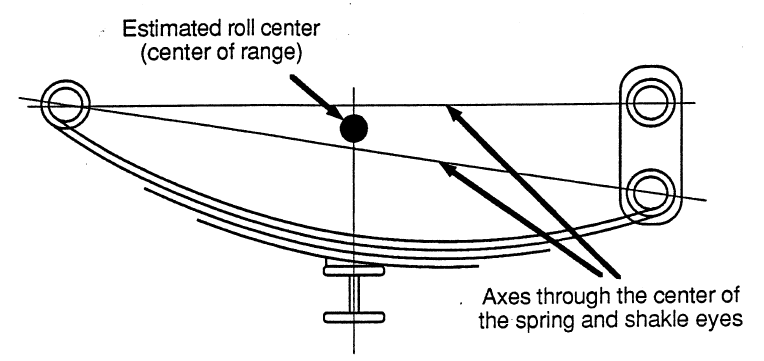
\includegraphics[height=1.2in]{fig/winkler-2011_roll-centre-estimation_typical-front-axle-suspensions}
		\caption{Typical front axle suspensions}
	\end{subfigure}
	\hfill
	\begin{subfigure}[t]{0.45\textwidth}
		\centering
		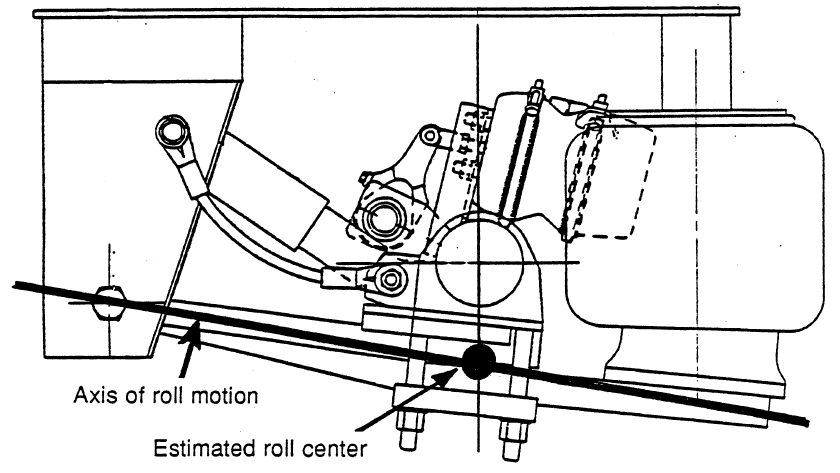
\includegraphics[height=1.2in]{fig/winkler-2011_roll-centre-estimation_compliant-trailing-arm-suspensions}
		\caption{Typical trailing arm suspensions}
	\end{subfigure}
	\caption{Estimate of roll centre heights for typical suspension configurations \cite{Winkler2011}}
	\label{figure:estimate-of-roll-centre-heights-for-typical-suspension-configurations}
\end{figure*}

The maximum axle cross section in the BPW rigid axles catalogue \cite{BPW2010} is 150~mm. Thus, assuming a maximum trailing arm thickness at the location of the axle of 100~mm to account for mounting plates, the maximum roll centre height from the centre of the axle is 125~mm below when the suspension is overslung and above when underslung as shown in Figure~\ref{figure:roll-centre-height-estimates-for-trailing-arm-suspension}.

%----------------------------------------------
%      FIGURE
%----------------------------------------------
\begin{figure*}[!htbp]
	\centering
	\begin{subfigure}[t]{0.45\textwidth}
		\centering
		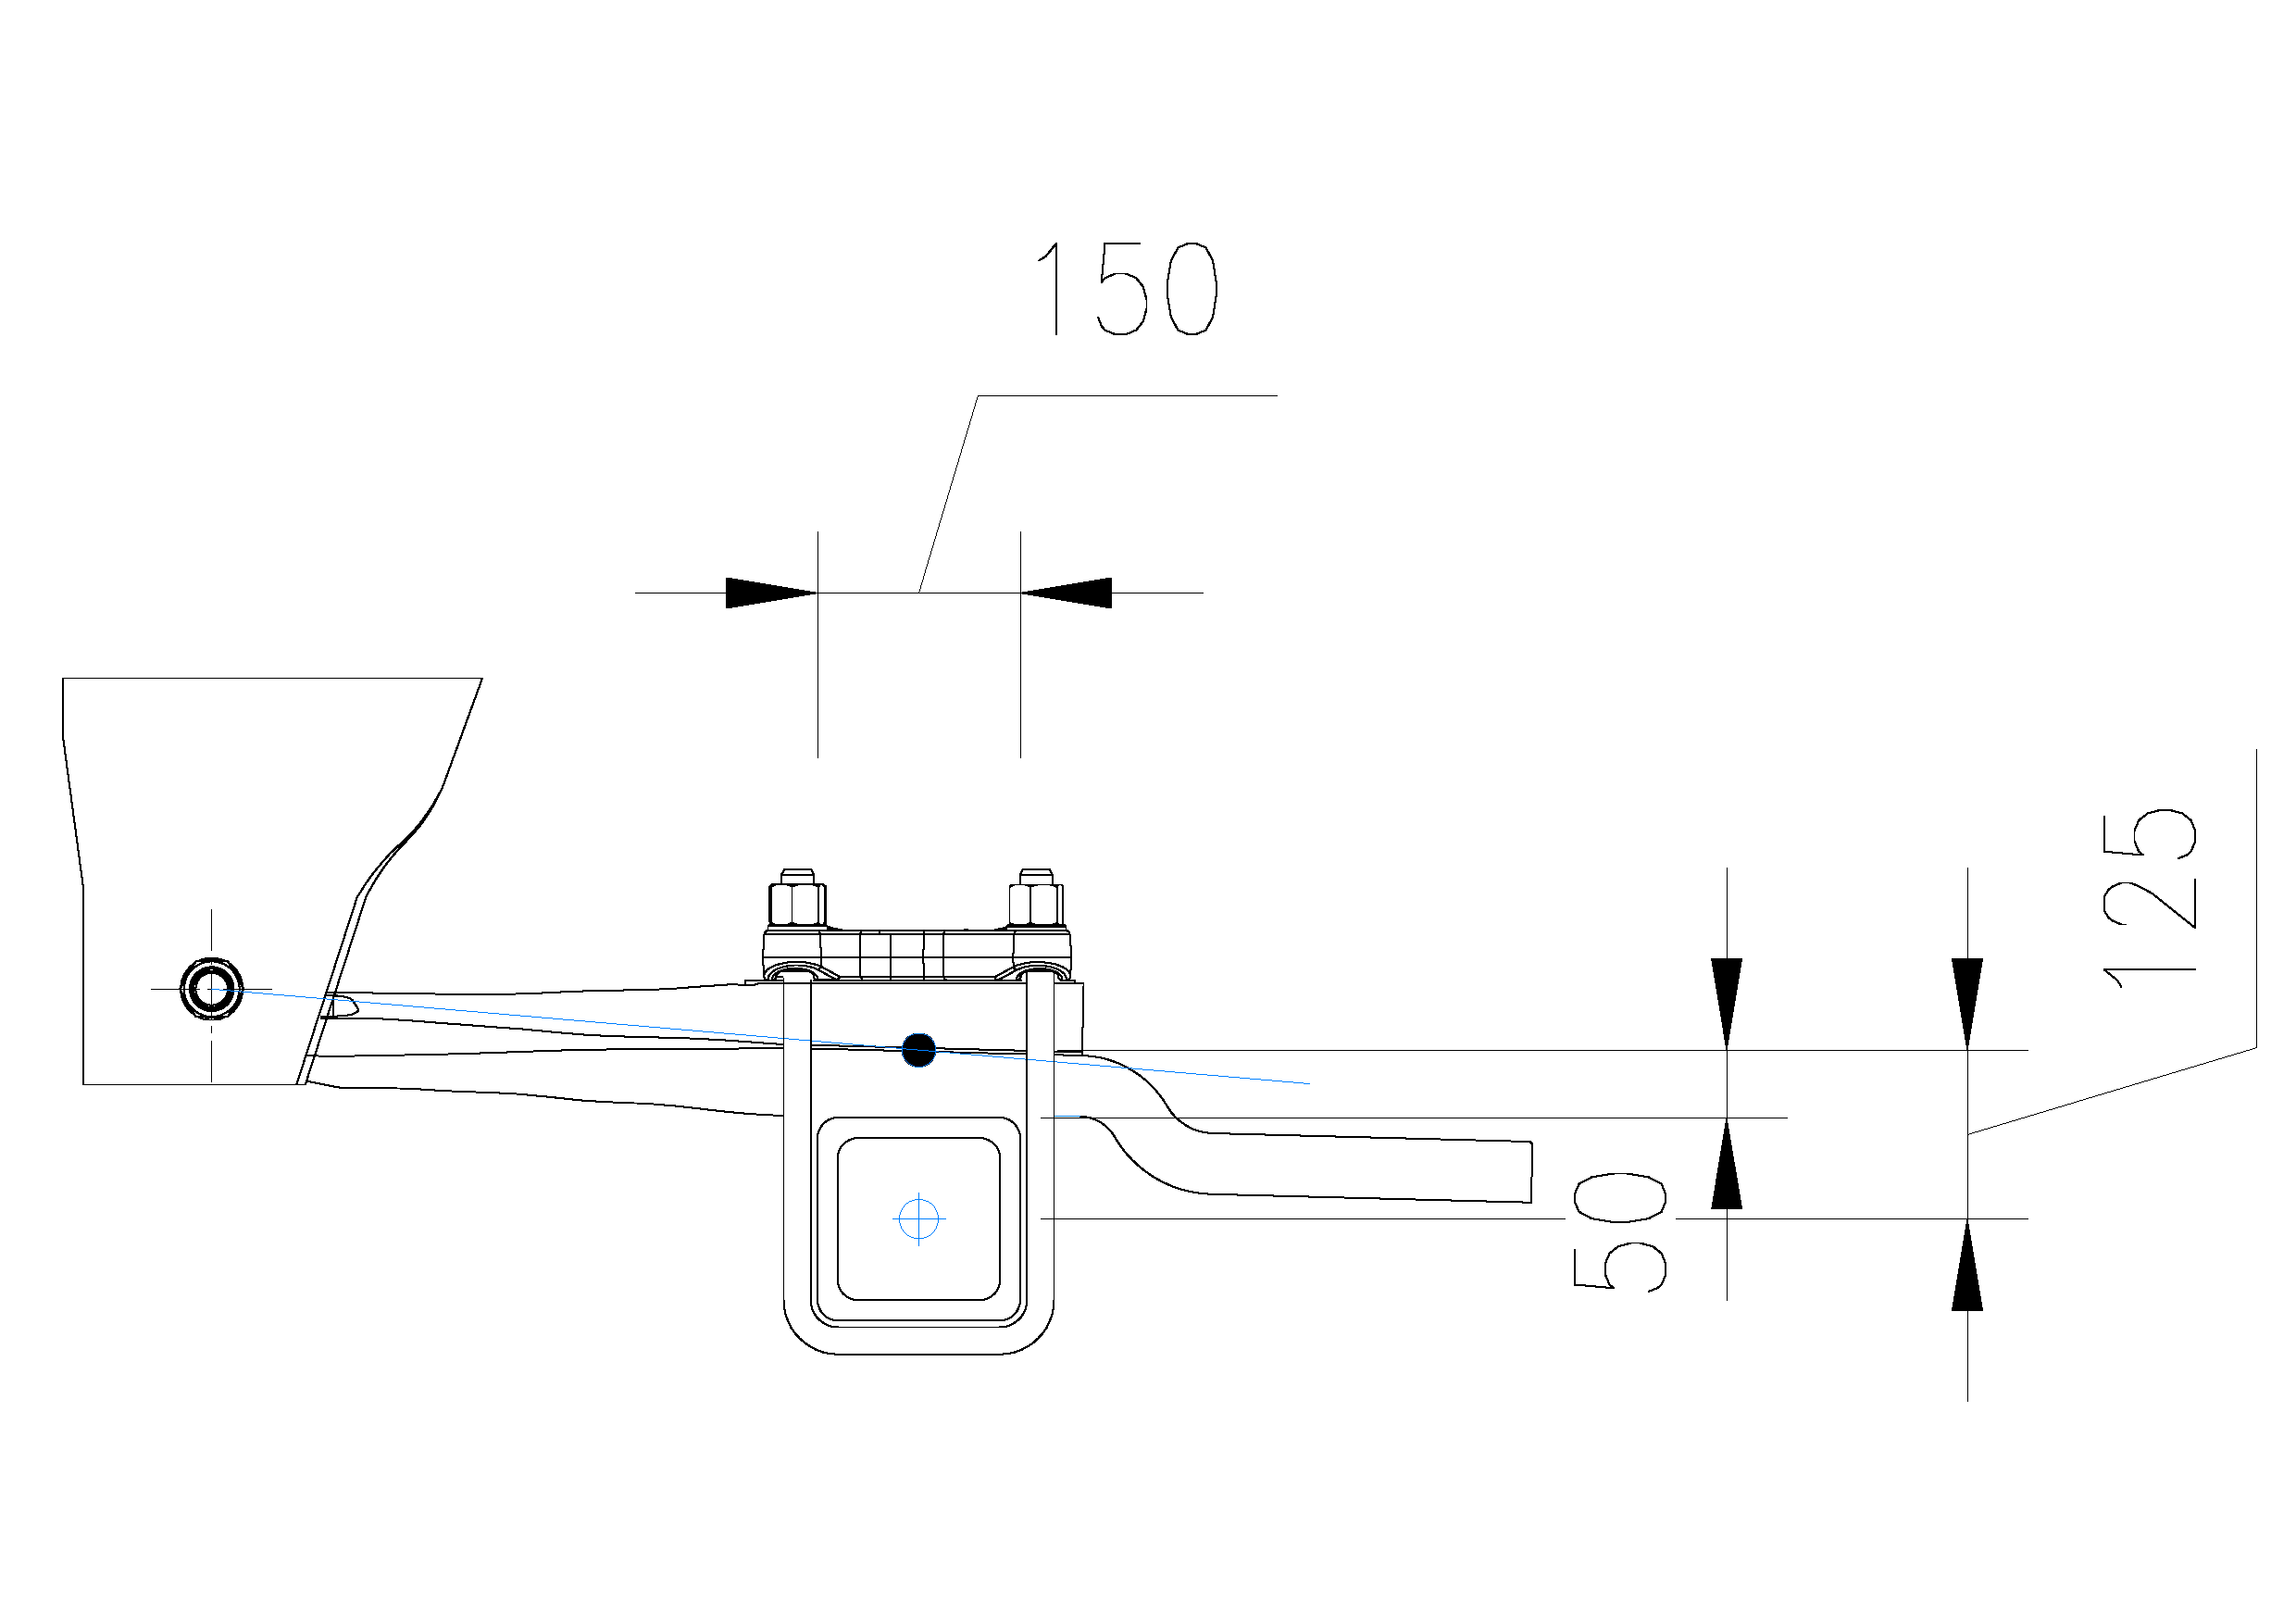
\includegraphics[width=1\textwidth]{fig/parameter-selection_roll-centre-height_overslung}
		\caption{Overslung (+125~mm)}
	\end{subfigure}\hfill
	\begin{subfigure}[t]{0.45\textwidth}
		\centering
		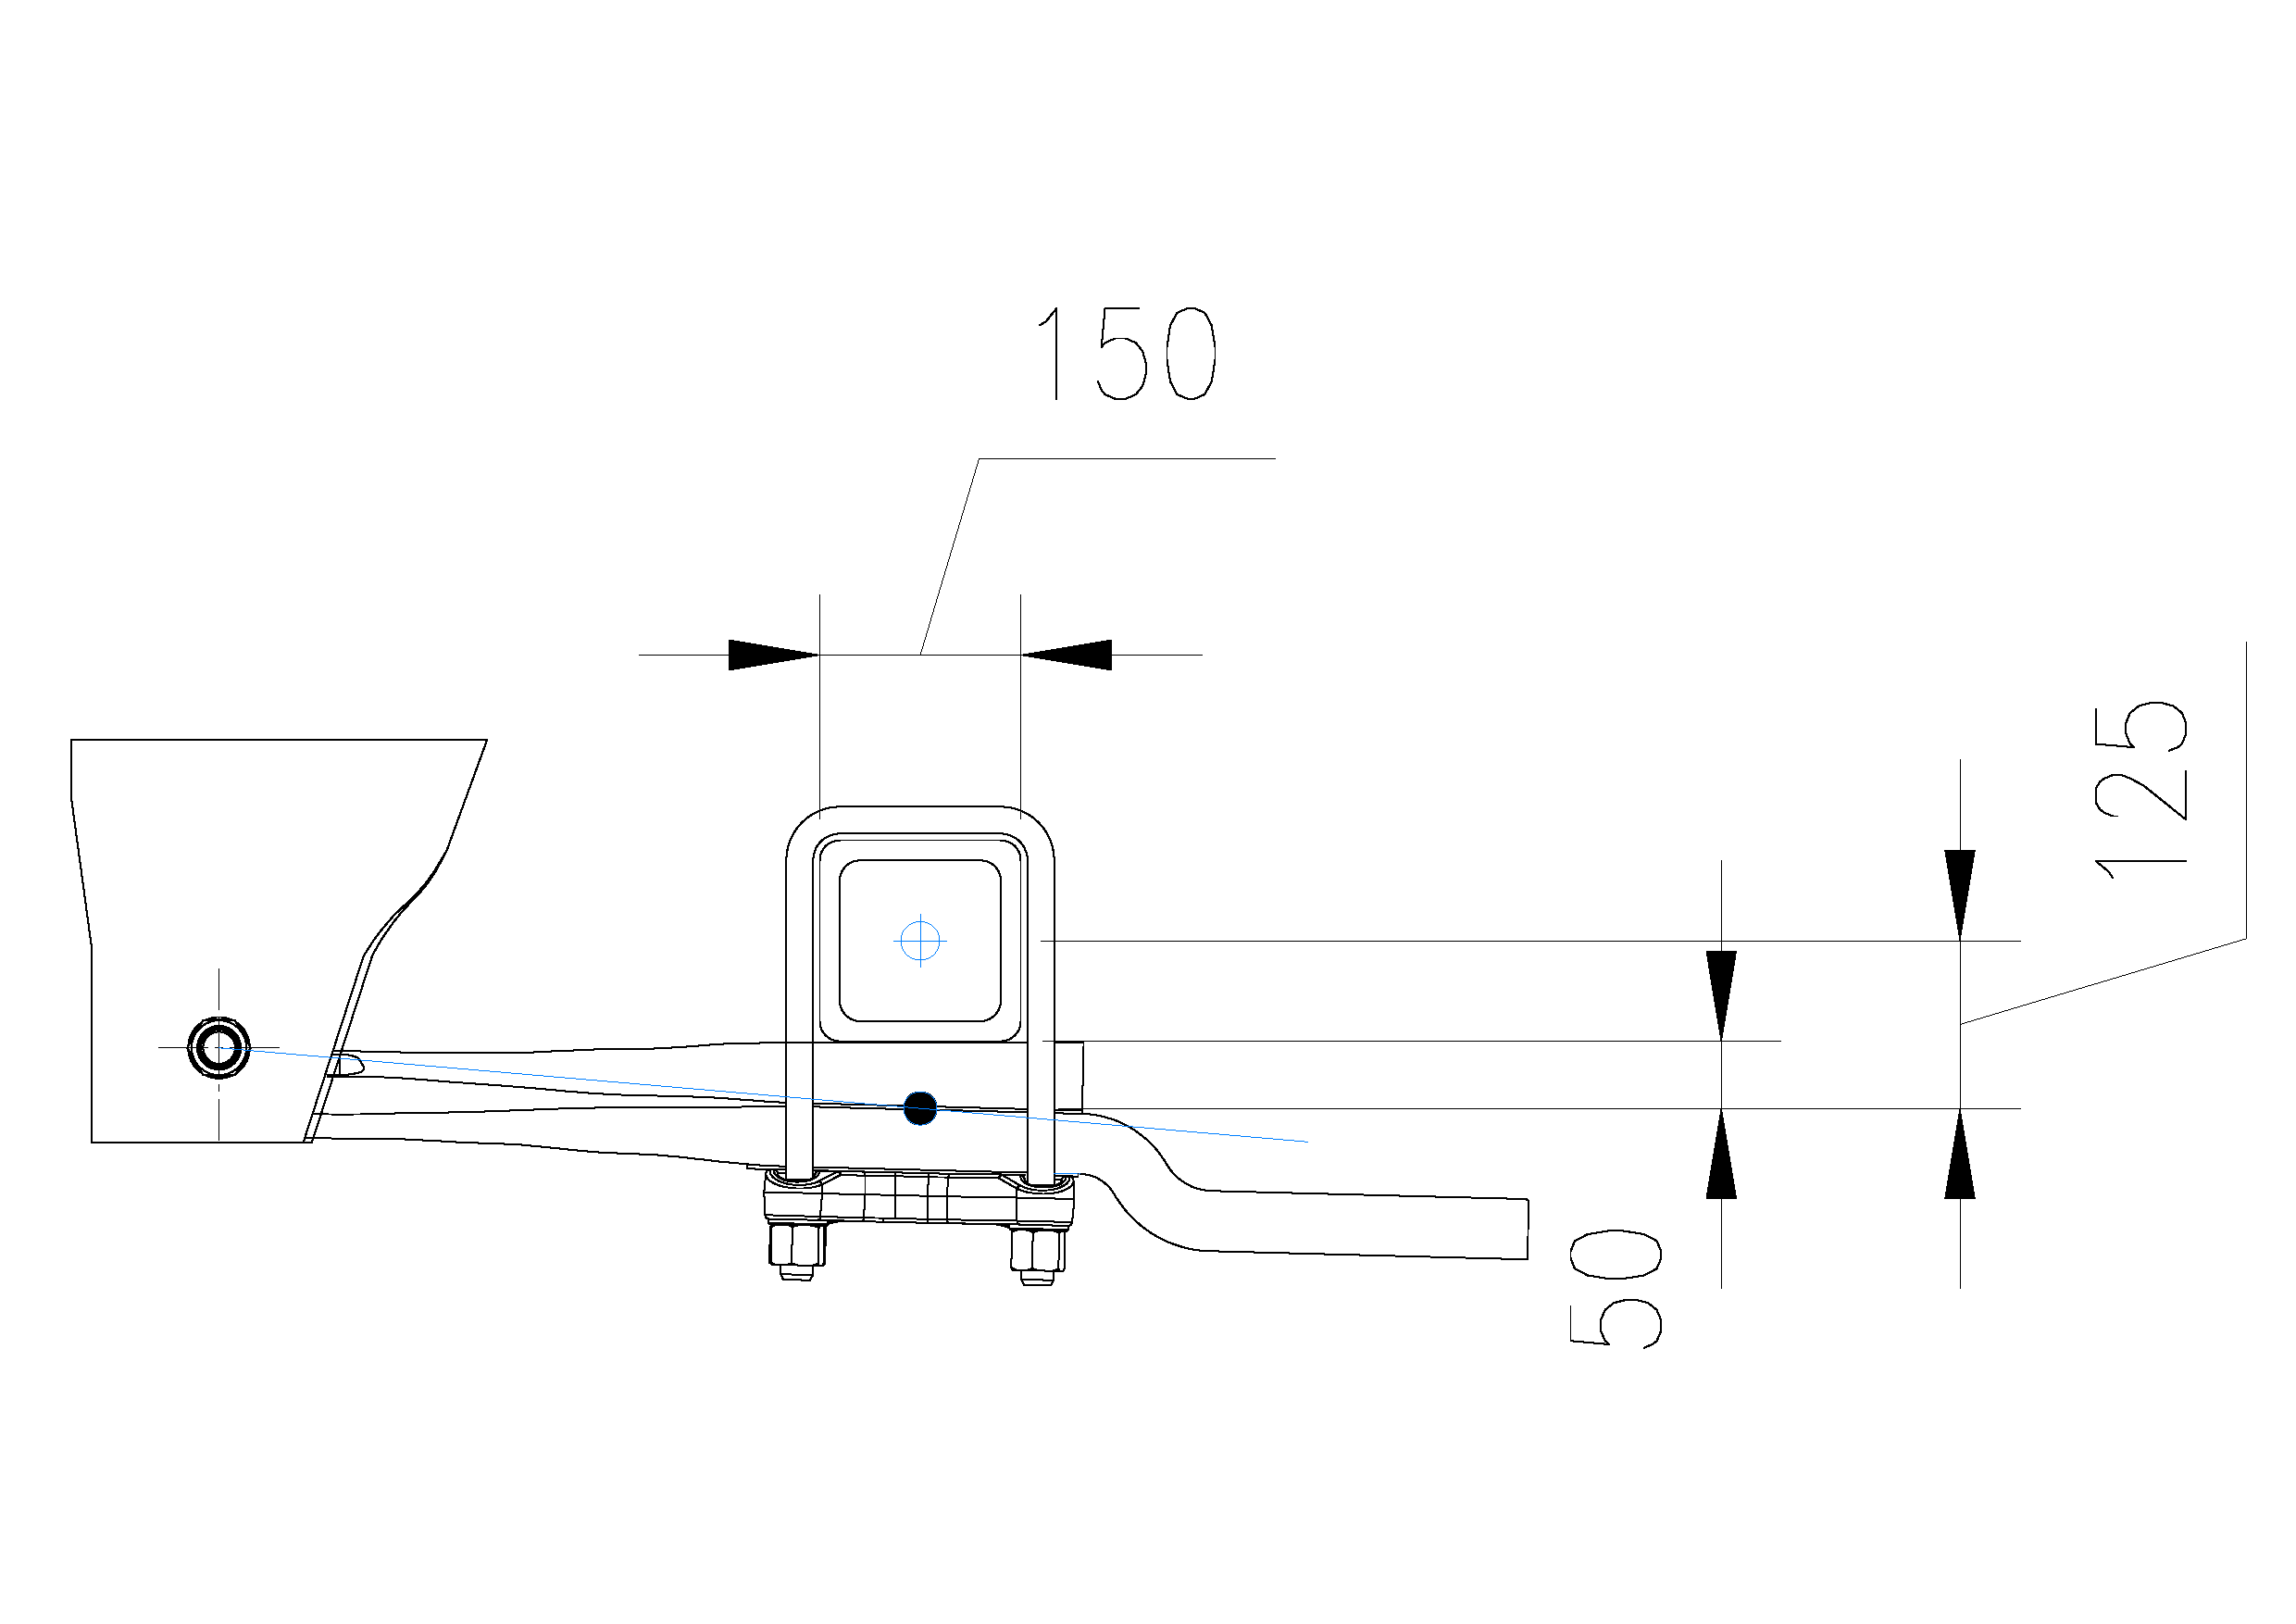
\includegraphics[width=1\textwidth]{fig/parameter-selection_roll-centre-height_underslung}
		\caption{Underslung (-125~mm)}
	\end{subfigure}

	\caption{Roll centre height estimates for trailing arm suspension}
	\label{figure:roll-centre-height-estimates-for-trailing-arm-suspension}
\end{figure*}
%----------------------------------------------
%      FIGURE
%----------------------------------------------

It is desirable from a stability perspective that the roll centre height be raised as high as possible. This is made possible with track bars as noted by Winkler et al. Thus, it was assumed with the use of additional lateral restraints such as a track bar that the maximum height of the roll centre above the trailing arm suspension could reach up to 200~mm.

The suspension used for baseline drive axle tandem bogie is of the A-frame type which  is laterally constrained on the chassis, leading to a high roll centre height of 400~mm above the wheel centre height. An illustration of this type of suspension is included from a Volvo data sheet for the Volvo RADD-GR \cite{VolvoTruckCorporation2012} suspension in Figure~\ref{figure:volvo-radd-gr-rear-axle-installation}.

%----------------------------------------------
%      FIGURE
%----------------------------------------------
\begin{figure}[H]
	\centering
	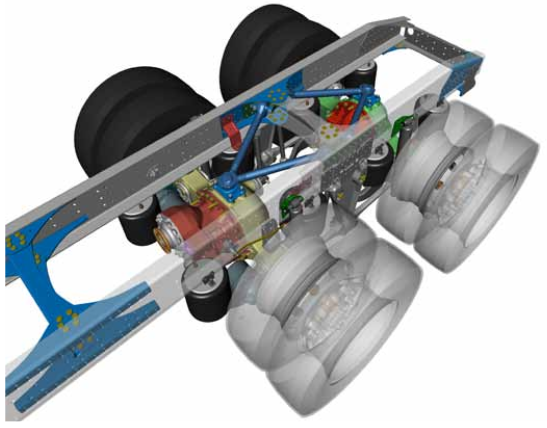
\includegraphics[width=0.5\textwidth]{fig/volvo_radd-gr-bogie-drive-axle-suspension}
	\caption{Volvo RADD-GR rear axle installation}
	\label{figure:volvo-radd-gr-rear-axle-installation}
\end{figure}
%----------------------------------------------
%      FIGURE
%----------------------------------------------

The baseline value of 400~mm was assumed as the maximum height, while the minimum roll centre height was assumed to be the same as for the trailer axles to evaluate the performance with various drive axle suspension designs.

The roll centre height of the steel steer axle suspension is governed by the geometry of the leaf springs as shown by the graphical estimation in Figure~\ref{figure:estimate-of-roll-centre-heights-for-typical-suspension-configurations}. The TERNZ SRT calculator \cite{TERNZTransportResearch} uses a roll centre height of 20~mm below the wheel centre for generic suspensions which was assumed as the minimum. A reasonable maximum was assumed to be 100~mm above the axle centre. The roll centre heights for front air suspension are typically near the axle centre (evident from \gls{oem} data) which was deemed to be representative of both front air and steel suspension designs.

%----------------------------------------------
%      TABLE - UPDATED TO NEW RANGES
%----------------------------------------------
\begin{table}[H]
	\centering\footnotesize
	\begin{threeparttable}

		\begin{tabulary}{\textwidth}{lccc}
			\toprule
			\textbf{Axle} & \textbf{Baseline (mm)\tnote{1}} & \textbf{Min. (mm)} & \textbf{Max. (mm)} \\
			\midrule
             Steer & +21    & -20   & +100 \\
             Drive & +400   & -125  & +400 \\
             Trailer & +114   & -125  & +200 \\
			\bottomrule
		\end{tabulary}

		\caption{Parameter range - roll centre height}
		\label{table:parameter-range-roll-centre-height}

		\begin{tablenotes}
			\item[1] Roll centre height is reported relative to the wheel centre height
		\end{tablenotes}

	\end{threeparttable}
\end{table}
%----------------------------------------------
%      TABLE
%----------------------------------------------

%      SUBSECTION
%----------------------------------------------
\section{Tyre Parameter Limits}\label{section:pr-tyre-properties}

Tyre data is well protected by \glspl{oem} and they are often not willing to disclose measured tyre test data. \gls{pbs} assessments are currently performed using conservative tyre data for lateral tyre force as extracted from \cite{Fancher1981}. This data is from 1981 and modern tyres are expected to have improved properties with advances in material and construction. The use of conservative data aligns with the NTC requirements that worst-case tyre data be used in the absence of measured data for the tyres in question \cite{NationalTransportCommission2008}.

Historically, both bias and radial ply tyres have been used on commercial heavy vehicles. However heavy trucks have been phasing out bias ply in favour of radial ply tyres since 1984 as mentioned by Ervin et al. \cite{Ervin1986}. All modern heavy commercial vehicles use radial ply tyres and hence the mechanical properties of bias ply tyres were not considered.

%      SUBSECTION
%----------------------------------------------
\subsection{Effective Rolling Radius}\label{section:pr-effective-rolling-radius}

The rolling radius is influenced by a multitude of operational factors such as the state of tyre wear, inflation pressure and speed. The effective rolling radius can be estimated from the unloaded tyre radius according to Genta \cite{Giancarlo1997} as 98\% of the unladen tyre radius.

The effective rolling radius for the baseline tyre models was calculated from the Michelin data book \cite{Michelin} using the supplied rolling circumference for each tyre. The effective rolling radius as a percentage of the unladen radius was calculated and it is shown in Table~\ref{table:effective-rolling-radius-of-baseline-tyre-models} that it is approximately 95\% of the unladen radius, with the 445/65 R22.5 tyre model having the lowest ratio of 94.5\%.

%----------------------------------------------
%      TABLE - UPDATED TO NEW RANGES
%----------------------------------------------
\begin{table}[H]
	\centering\footnotesize
	\begin{threeparttable}

		\begin{tabulary}{\textwidth}{lccc}
			\toprule
    \textbf{Tyre} & \textbf{Unladen radius (mm)} & \textbf{Effective rolling radius (mm)} & \textbf{\% of unladen radius} \\

			\midrule
    445/65 R22.5 & 587   & 555   & 94.5\% \\
    315/80 R22.5 & 548   & 522   & 95.3\% \\
    285/70 R19.5 & 456   & 434   & 95.2\% \\
			\bottomrule
		\end{tabulary}

		\caption{Effective rolling radius of baseline tyre models}
		\label{table:effective-rolling-radius-of-baseline-tyre-models}

		%\begin{tablenotes}
		%\item[1] %\tnote{1}
		%\end{tablenotes}

	\end{threeparttable}
\end{table}
%----------------------------------------------
%      TABLE
%----------------------------------------------

Accounting for various operating conditions and considering the effective rolling ratios of the baseline combinations, it was assumed that the effective rolling radius could vary from 94\% to 98\% of the baseline unladen radius. The resulting range of effective rolling radii for each tyre is summarised in Table~\ref{table:pr-tyre-effective-rolling-radius}.

%----------------------------------------------
%      TABLE - UPDATED TO NEW RANGES
%----------------------------------------------
\begin{table}[H]
	\centering\footnotesize
	\begin{threeparttable}

		\begin{tabulary}{\textwidth}{lccc}
			\toprule
            \textbf{Tyre} & \textbf{Baseline (mm)} & \textbf{Min. (mm)} & \textbf{Max. (mm)} \\
			\midrule
            445/65 R22.5 & 555   & 552   & 575 \\
            315/80 R22.5 & 522   & 515   & 537 \\
            285/70 R19.5 & 434   & 429   & 447 \\
			\bottomrule
		\end{tabulary}

		\caption{Parameter range - tyre effective rolling radius}
		\label{table:pr-tyre-effective-rolling-radius}

		%\begin{tablenotes}
		%\item[1] %\tnote{1}
		%\end{tablenotes}

	\end{threeparttable}
\end{table}
%----------------------------------------------
%      TABLE
%----------------------------------------------

%      SUBSECTION
%----------------------------------------------
\subsection{Unloaded Radius}\label{section:pr-unloaded-radius}

Data collected from tyre manufacturer data books (Bridgestone \cite{Bridgestone2015}, Goodyear \cite{Goodyear} and Michelin \cite{Michelin}) and summarised in Tables~\ref{table:spring-rate-approximation-for-445-65R22.5-tyres}~to~\ref{table:spring-rate-approximation-for-285/70 R19.5-tyres} in Appendix~\ref{section:tyre-spring-rate} were consulted to determine the variation in unloaded radii between manufacturers. The range of unloaded radii evaluated is summarised in Table~\ref{table:pr-tyre-unloaded-radius}.

%----------------------------------------------
%      TABLE - UPDATED TO NEW RANGES
%----------------------------------------------
\begin{table}[H]
	\centering\footnotesize
	\begin{threeparttable}

		\begin{tabulary}{\textwidth}{lccc}
			\toprule
			\textbf{Tyre} & \textbf{Baseline (mm)} & \textbf{Min. (mm)} & \textbf{Max. (mm)} \\
			\midrule
            445/65 R22.5 & 587   & 575   & 589 \\
            315/80 R22.5 & 548   & 538   & 550 \\
			285/70 R19.5 & 456   & 448   & 456 \\
			\bottomrule
		\end{tabulary}

		\caption{Parameter range - tyre unloaded radius}
		\label{table:pr-tyre-unloaded-radius}

		%\begin{tablenotes}
		%\item[1] %\tnote{1}
		%\end{tablenotes}

	\end{threeparttable}
\end{table}
%----------------------------------------------
%      TABLE
%----------------------------------------------

%      SUBSECTION
%----------------------------------------------
\subsection{Tyre Spring Rate}\label{section:pr-tyre-spring-rate}

The vertical spring rate of each tyre model was calculated from the given axle load, considering the difference between the unladen and laden radius, the spring of the tyre was estimated assuming linear behaviour and using Equation~\ref{equation:hookes-law} (Hooke's law).

%----------------------------------------------
%      EQUATION
%----------------------------------------------
\begin{align}
	\label{equation:hookes-law}
	\gls{tyrespringrate}=\frac{\gls{fz}}{\Delta{}x}
\end{align}

Where:

\gls{tyrespringrate} = Tyre spring rate (N/mm)

\gls{fz} = Vertical tyre load (N)

\gls{deltax} = Tyre deflection (mm)

%----------------------------------------------
%      EQUATION
%----------------------------------------------

Tyre spring rates were calculated from the data from Bridgestone, Goodyear and Michelin \cite{Bridgestone2015,Goodyear,Michelin} for dual and single tyre arrangements at various pressures and axle loads. Tables~\ref{table:spring-rate-approximation-for-445-65R22.5-tyres}~to~\ref{table:spring-rate-approximation-for-285/70 R19.5-tyres} in Appendix~\ref{section:tyre-spring-rate} include the calculated tyre spring rates. The resulting range of tyre spring rates evaluated is summarised in Table~\ref{table:parameter-range-vertical-tyre-stiffness}.

%----------------------------------------------
%     TABLE - UPDATED TO NEW RANGES
%----------------------------------------------
\begin{table}[H]
	\centering\footnotesize
	\begin{threeparttable}

		\begin{tabulary}{\textwidth}{lccc}
			\toprule
			\textbf{Tyre} & \textbf{Baseline (N/mm)} & \textbf{Min. (N/mm)} & \textbf{Max (N/mm)} \\

			\midrule
             445/65 R22.5 & 1193  & 773   & 1237 \\
             315/80 R22.5 & 987   & 565   & 1169 \\
             285/70 R19.5 & 801   & 473   & 901 \\		

			\bottomrule
		\end{tabulary}

		\caption{Parameter range - tyre spring rate}
		\label{table:parameter-range-vertical-tyre-stiffness}

		%\begin{tablenotes}
		%\item[1] %\tnote{1}
		%\end{tablenotes}

	\end{threeparttable}
\end{table}
%----------------------------------------------
%      TABLE
%----------------------------------------------

\subsection{Wheel and Tyre Assembly Spin Moment of Inertia}\label{section:pr-tyre-spin-moment-of-inertia}

Spin inertias for wheel and tyre assemblies were derived as 10 kg.m\sstw{} for 19.5" wheels and 12 kg.m\sstw{} for 22.5" wheels by de Saxe \cite{DeSaxe2012} from UMTRI data \cite{Winkler1995}, \cite{Winkler1983}. This correlates well with the \trucksim{} database which has values of 13 kg.m\sstw{} (\textit{2000~kg rating, 425 mm Radius (Drive)}) to 28 kg.m\sstw{} (\textit{SAE Widebase, 4750~kg})  for truck tyres. 

It was assumed that the above data are for steel rims. Thus, considering aluminium rims (approximately half the weight of a steel rim) and additional weight reductions in modern designs, the minimum spin moment of inertia was calculated with a reduction in wheel assembly mass of 50\%. The evaluated range of wheel and tyre assembly spin moment of inertias is summarised in Table~\ref{table:pr-wheel-assembly-spin-moment-of-inertia}.

%----------------------------------------------
%      TABLE - UPDATED TO NEW RANGES
%----------------------------------------------
\begin{table}[H]
	\centering\footnotesize
	\begin{threeparttable}

		\begin{tabulary}{\textwidth}{lccc}
			\toprule
    \textbf{Tyre} & \textbf{Baseline (kg.m\sstw{})} & \textbf{Min. (kg.m\sstw{})} & \textbf{Max. (kg.m\sstw{})} \\
			\midrule
    285/70 R19.5 & 10    & 6.5   & 13 \\
    315/80 R22.5 & 12    & 7     & 14 \\
    445/65 R22.5 & 28    & 14    & 28 \\
			\bottomrule
		\end{tabulary}

		\caption{Parameter range - wheel and tyre assembly spin moment of inertia}
		\label{table:pr-wheel-assembly-spin-moment-of-inertia}

		%\begin{tablenotes}
		%\item[1] %\tnote{1}
		%\end{tablenotes}

	\end{threeparttable}
\end{table}
%----------------------------------------------
%      TABLE
%----------------------------------------------

\subsection{Tyre Lag (relaxation length)}\label{section:pr-tyre-lag}
Literature defining truck tyre lag (also known as relaxation length) ranges could not be found, however\trucksim{} indicates that reasonable estimates of  tyre lag are as follows:

\begin{itemize}
	\item \gls{lagfx} (longitudinal tyre lag): 1/10 of the tyre radius
	\item \gls{lagfymz} (lateral tyre lag): Twice the tyre radius
\end{itemize}

The NTC standards and vehicle assessment rules for the PBS framework \cite{NationalTransportCommission2008} do not clearly state whether the simulated vehicle performance should include the effects of tyre lag. Thus tyre lag was varied from the recommended value down to values that would effectively simulate zero tyre lag to evaluate the impact of including the effects of tyre lag in the vehicle simulations.

When tyre lag is set to absolute zero, the driver model is unstable. To simulate zero tyre lag (on all but the steer tyres - see footnote \textsuperscript{1} in Table~\ref{table:parameter-range-tyre-lag}) without causing instabilities in the driver model, resulting in erroneous vehicle performance, the following parameters were used.

\begin{itemize}
	\item \gls{lagfx}: remains at approximately 1/10 of the tyre radius
	\item \gls{lagfymz} : reduced to 100~mm
\end{itemize}

The resulting range of tyre lag values are presented in Table~\ref{table:parameter-range-tyre-lag}.

%----------------------------------------------
%     TABLE - UPDATED TO NEW RANGES
%----------------------------------------------
\begin{table}[H]
	\centering\footnotesize
	\begin{threeparttable}

		\begin{tabulary}{\textwidth}{lccc}
			\toprule
			\textbf{Tyre} & \textbf{Baseline (mm / mm)} & \textbf{Min. (mm / mm)} & \textbf{Max. (mm / mm)} \\
			\midrule
			445/65 R22.5 & 55 / 1100 & 55 / 100 & 55 / 1100 \\
			315/80 R22.5\tnote{1} & 50 / 1000 & 50 / 100 & 50 / 1000 \\
			285/70 R19.5 & 45 / 900 & 45 / 100 & 45 / 900 \\
			\bottomrule
		\end{tabulary}

		\caption{Parameter range - tyre lag (\gls{lagfx} / \gls{lagfymz})}
		\label{table:parameter-range-tyre-lag}

		\begin{tablenotes}
			\item[1] The steer tyre lag is set to 50/1 to prevent instabilities with the driver model. Lag response in the steer tyre causes the driver to overcompensate for the lagged response after a steering input, resulting in instability.
		\end{tablenotes}

	\end{threeparttable}
\end{table}
%----------------------------------------------
%      TABLE
%----------------------------------------------

\subsection{Tyre Cornering Stiffness}\label{section:pr-tyre-cornering-stiffness}

Cornering stiffness tyre data is not readily supplied by manufacturers and could not be used to determine the possible range of tyre data. Conservative tyre models sourced from measured tyre performance provided by \gls{umtri} in studies performed by Fancher \cite{Fancher1981} and Bogard et al. \cite{Bogard1991} are generally used in PBS assessments in South Africa. These same tyre models were used for the baseline combinations.

Fancher et al. \cite{Fancher1986} measured cornering stiffness at rated load for a range of tyres and measured that tyre wear of 1/3 of the tread depth can yield an increase in cornering stiffness of approximately 0.04. This measured data was compared with the cornering stiffness of the baseline combinations to gauge a range of cornering stiffness that should be considered (including the effect of increased cornering stiffness with tyre wear).

The steer, drive and trailer tyres were evaluated separately to provide insight into how using tyres of varying cornering stiffness on the same combination could influence behaviour as well as yield insight into the sensitivity of vehicle performance to the cornering stiffness of the tyres. Situations like this can occur when worn tyres are rotated from the prime mover to the trailer or retreads of unknown cornering stiffness properties are used.

The cornering stiffness was calculated within the linear region of each tyre for the same vertical loading at which the tyres were tested by Fancher et al. of 26879~N (6040 Lbs). The cornering stiffness was then normalised with the vertical tyre load according to Equation~\ref{equation:cornering-coefficient} to determine the cornering coefficient which could then be compared to the data provided by Fancher et al.

%----------------------------------------------
%      EQUATION
%----------------------------------------------
\begin{align}
	\label{equation:cornering-coefficient}
	C_{c} = \frac{C_{\alpha{}}}{F_z}
\end{align}

Where:

\gls{ccornering} = Cornering coefficient (\degree{}\textsuperscript{-1})

\gls{calpha} = Cornering stiffness (N/\degree{})

\gls{fz} = Vertical tyre load (N)

%----------------------------------------------
%      EQUATION
%----------------------------------------------

The variation for the cornering stiffness values are summarised in Table~\ref{table:cornering-stiffness-variation}. The baseline cornering stiffness values are conservative in relation to the cornering stiffness values measured by Fancher et al. \cite{Fancher1986}. This is in-line with the requirements of the NTC for PBS assessments which state \cite{NationalTransportCommission2008} that if no tyre data is available, conservative worst-case tyre data must be used.

Using the variations as a guideline, a conservative range of cornering stiffness values relative to the baseline models were evaluated as per Table~\ref{table:pr-tyre-cornering-stiffness}. 

%----------------------------------------------
%      TABLE - UPDATED TO NEW RANGES
%----------------------------------------------
\begin{table}[H]
	\centering\footnotesize
	\begin{threeparttable}

		\begin{tabulary}{\textwidth}{lcccccCC}
			\toprule
			\textbf{Tyre} & \textbf{Load} & \boldmath{}\textbf{$C_\alpha{}$ (N/\degree{})}\unboldmath{} & \boldmath{}\textbf{$C_c$ (/\degree{})}\unboldmath{} & \boldmath{}\textbf{Min. $C_c$ (/\degree{})\tnote{1}}\unboldmath{} & \boldmath{}\textbf{Max. $C_c$ (/\degree{})\tnote{1} \textsuperscript{,} \tnote{2}}\unboldmath{} & \textbf{Min.\tnote{3}} & \textbf{Max.\tnote{3}} \\
			\midrule
			445/65 & 26879 & 2886  & 0.1074 & 0.1121 & 0.1861 & 104\% & 173\% \\
			315/80 & 26879 & 2775  & 0.1033 & 0.1121 & 0.1861 & 109\% & 180\% \\
			285/70 & 26879 & 3115  & 0.1159 & 0.1121 & 0.1861 & 97\%  & 161\% \\
			\bottomrule
		\end{tabulary}

		\caption{Cornering stiffness variation}
		\label{table:cornering-stiffness-variation}

		\begin{tablenotes}
		\item[1] Including the effects of tyre wear (additional 0.04 to the cornering coefficient)
		\item[2] Fancher et al. \cite{Fancher1986}
		\item[3] Variation relative to the baseline cornering coefficient
		\end{tablenotes}

	\end{threeparttable}
\end{table}
%----------------------------------------------
%      TABLE
%----------------------------------------------

%----------------------------------------------
%      TABLE - UPDATED TO NEW RANGES
%----------------------------------------------
\begin{table}[H]
	\centering\footnotesize
	\begin{threeparttable}

		\begin{tabulary}{\textwidth}{lccc}
			\toprule
			\textbf{Tyre} & \textbf{Baseline\tnote{1}} & \textbf{Min.} & \textbf{Max.} \\
			\midrule
			445/65 R22.5 & 100\% & 100\% & 173\% \\
			315/80 R22.5 & 100\% & 100\% & 180\% \\
			285/70 R19.5 & 100\% & 97\%  & 161\% \\

			\bottomrule
		\end{tabulary}

		\caption{Parameter range - tyre cornering stiffness}
		\label{table:pr-tyre-cornering-stiffness}

		\begin{tablenotes}
		\item[1] The cornering stiffness is reported as a percentage of the baseline value
		\end{tablenotes}

	\end{threeparttable}
\end{table}
%----------------------------------------------
%      TABLE
%----------------------------------------------

Scaling the baseline tyre data causes the coefficient of friction for the data to be skewed to unrealistic values and this results in the tyre lateral force saturating at unrealistically low slip angles. To prevent this, the baseline tyre models were converted to equivalent Pacejka '89 models \cite{Bakker1989}. The Pacejka '89 models were then scaled by manipulating the maximum cornering stiffness shape factor ($a3$) within the tyre cornering stiffness range in Table~\ref{table:pr-tyre-cornering-stiffness} to generate more realistically scaled tyre curves.

\subsection{Dual Tyre Spacing}\label{section:pr-dual-tyre-spacing}

Minimum dual tyre spacing is quoted by tyre \glspl{oem} to ensure that the tyres do not touch during operation which would severely reduce the tyre life as well as become a fire risk.

Minimum dual tyre spacing for the 315/80 R22.5 and 285/70 R19.5 dual tyre assemblies were found in the \gls{oem} data books from Michelin, Goodyear and Bridgestone \cite{Michelin,Goodyear,Bridgestone2015} and are reported in Table~\ref{table:minimum-dual-tyre-spacings}. In general the minimum spacings are similar, with a maximum difference of 4~mm between \glspl{oem}.

The dual spacing of the baseline vehicles was modelled on the Michelin data, which is consistently the minimum between all manufactures. Thus, assuming that a standard 5~mm plate can be used as a spacer between rims to account for various tyre models, the baseline dual tyre spacing was varied from the baseline value to a maximum of 5~mm additional spacing as per Table~\ref{table:pr-dual-tyre-spacing}.

%----------------------------------------------
%      TABLE - UPDATED TO NEW RANGES
%----------------------------------------------
\begin{table}[H]
	\centering\footnotesize
	\begin{threeparttable}

		\begin{tabulary}{\textwidth}{lccc}
			\toprule
            \textbf{Tyres} & \textbf{Michelin} & \textbf{Goodyear} & \textbf{Bridgestone} \\
			\midrule
               
            315/80 R22.5 & 350   & 351   & 350.5 \\
            285/70 R19.5 & 314   & 318   & 317.5 \\
			
            \bottomrule
		\end{tabulary}

		\caption{Minimum dual tyre spacings}
		\label{table:minimum-dual-tyre-spacings}

		%\begin{tablenotes}
		%\item[1] \tnote{1}
		%\end{tablenotes}

	\end{threeparttable}
\end{table}
%----------------------------------------------
%      TABLE
%----------------------------------------------

%----------------------------------------------
%      TABLE - UPDATED TO NEW RANGES
%----------------------------------------------
\begin{table}[H]
	\centering\footnotesize
	\begin{threeparttable}

		\begin{tabulary}{\textwidth}{lccc}
			\toprule
            \textbf{Tyres} & \textbf{Baseline (mm)} & \textbf{Minimum (mm)} & \textbf{Maximum (mm)} \\
			\midrule  
    		
            315/80 R22.5 & 350   & 350   & 355 \\
            285/70 R19.5 & 314   & 314   & 319 \\
			
            \bottomrule
		\end{tabulary}

		\caption{Parameter range - dual tyre spacing}
		\label{table:pr-dual-tyre-spacing}

		%\begin{tablenotes}
		%\item[1] \tnote{1}
		%\end{tablenotes}

	\end{threeparttable}
\end{table}
%----------------------------------------------
%      TABLE
%----------------------------------------------
\chapter{Results}\label{chapter:results}

To quantify the influence of each \gls{vdp} on the performance of a baseline combination for a particular PBS performance measure, the coefficient of variation (\gls{cv}) metric was used. The \gls{cv} facilitates the comparison of datasets where the units of measurement may differ \cite{Soong2004} and is a measure of the spread of data about its mean.

Each \gls{vdp} was systematically varied in isolation with 5 equally distributed data points ranging from the minimum to the maximum value as per the ranges developed in Section~\ref{chapter:parameter-range-selection}. For each \gls{vdp}, the \gls{cv} of each PBS performance measure was calculated as per Equation~\ref{equation:cv}.

%----------------------------------------------
%      EQUATION
%----------------------------------------------
\begin{equation}
    \label{equation:cv}
    CV = \frac{\sigma}{\mu} \times 100\%
\end{equation}
%----------------------------------------------
%      EQUATION
%----------------------------------------------

To compare the relative influence of each \gls{vdp} on each \gls{pbs} performance measure, the \gls{cv} for each \gls{pbs} performance measure was normalised with respect to the parameter with the highest \gls{cv} ($CV_{max}$). Thus the \gls{cv} matrix columns are normalised according to $CV_{max}$ for that column and the normalised values are denoted as $CV_n$ as per Equation \ref{equation:cv-norm}.

%----------------------------------------------
%      EQUATION
%----------------------------------------------
\begin{equation}
    \label{equation:cv-norm}
    CV_{n} = \frac{CV}{CV_{max}} \times 100\%
\end{equation}
%----------------------------------------------
%      EQUATION
%----------------------------------------------

%----------------------------------------------
%      EQUATION
Where:
\begin{itemize}[label={}]
\item $\sigma$ = standard deviation for a single performance measure evaluated for a single \gls{vdp}
\item $\mu$ = mean performance for a single performance measure evaluated for a single \gls{vdp}
\item $CV$ = coefficient of variation for a single performance measure evaluated for a single \gls{vdp}
\item $CV_n$ = normalised coefficient of variation for a single performance measure evaluated for a single \gls{vdp}
\item $CV_{max}$ = maximum coefficient of variation observed for a single performance measure (each column in the \gls{cv} matrix represents a single performance measure)
\end{itemize}
%      EQUATION
%----------------------------------------------

Any parameter that produced a $CV_n$ of less than 10\% (i.e. a \gls{cv} less than 10\% of the maximum coefficient of variation for the same performance measure) for a performance measure was regarded as having a negligible relative influence and was omitted from the overall \gls{cv} matrices in Section~\ref{sec:results-overall}. A set of complete \gls{cv} matrices containing all evaluated \glspl{vdp} are included in Sections~\ref{section:complete-cv-quad-semi}~to~\ref{section:complete-cv-rigid-drawbar}. Additional matrices comparing the relative influence of the inertial, geometrical, suspension and tyre \glspl{vdp} in isolation can be found in Appendices~\ref{section:cv-geometrical}~to~\ref{section:cv-tyre}.

\section{Interpretation of the CV Matrix}\label{section:interpretation-of-the-results-matrix}

The columns of the \gls{cv} matrices represent \gls{pbs} performance measures and the rows represent \glspl{vdp}. The numerical value in a cell represents the \gls{cvn} for the \gls{vdp} described in that row with respect to the \gls{pbs} performance described in that column.

In a single column, the influence of each \gls{vdp} on a \gls{pbs} performance measure is recorded relative to the \gls{vdp} that had the maximum influence on the \gls{pbs} performance measure according to Table~\ref{table:cv-matrix-conventions}. Each row indicates the relative influence of the described \gls{vdp} on each of the \gls{pbs} performance measures. An example of interpreting the \gls{cv} matrices is provided in Figure~\ref{figure:interpretation-of-cv-matrix}.

%----------------------------------------------
%      FIGURE
%----------------------------------------------
    \begin{figure}[H]
        \centering
        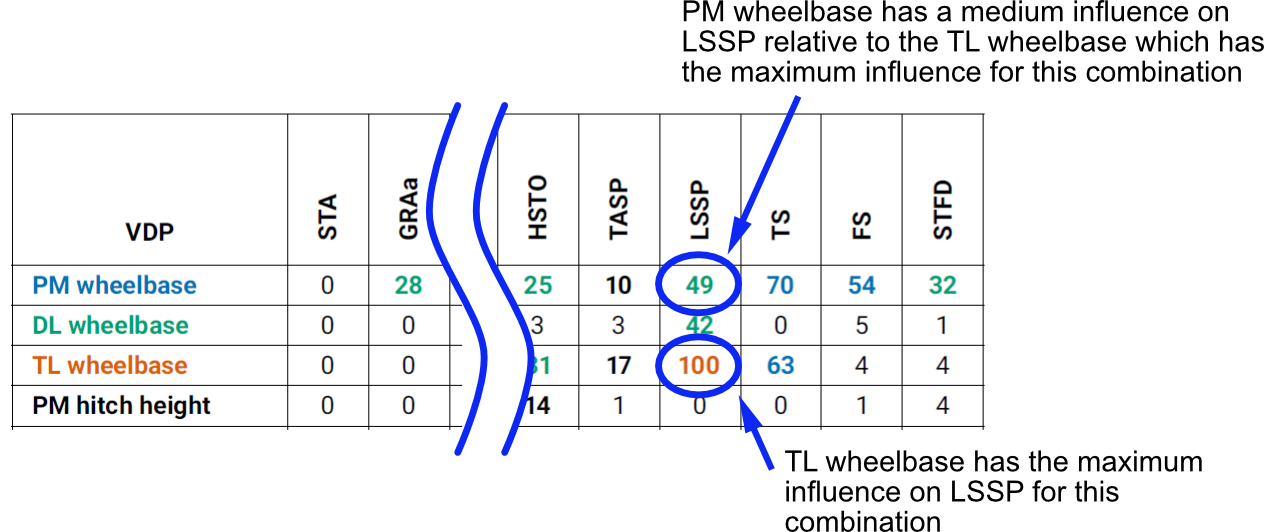
\includegraphics[width=1\textwidth]{fig/interpretation-of-cv-matrix}
        \caption{Interpretation of the \gls{cv} matrix}
        \label{figure:interpretation-of-cv-matrix}
    \end{figure}
%----------------------------------------------
%      FIGURE
%----------------------------------------------

To enhance the readability of the \gls{cv} matrices, the conventions and abbreviations detailed in Tables~\ref{table:cv-matrix-abbreviations}~to~\ref{table:cv-matrix-conventions} have been used throughout.

%----------------------------------------------
%      TABLE
%----------------------------------------------
\begin{table}[H]
	\centering\footnotesize
	\begin{threeparttable}

		\begin{tabulary}{\textwidth}{cl}
			\toprule
            
              \textbf{Abbreviation} & \textbf{Description}\\
              \midrule
              PM & Prime mover\\
              TL & Trailer\\
              St. & Steer axle\\
              Dr. & Drive axle\\
              Tl. & Trailer axle\\

			\bottomrule
		\end{tabulary}

		\caption{\gls{cv} matrix abbreviations}
		\label{table:cv-matrix-abbreviations}

		%\begin{tablenotes}
		%\item[1] %\tnote{1}
		%\end{tablenotes}

	\end{threeparttable}
\end{table}
%----------------------------------------------
%      TABLE
%----------------------------------------------

%-------------------------------------------------
%      TABLE

\begin{table}[H]
\centering\footnotesize
\begin{threeparttable}
\caption{CV matrix conventions}
\label{table:cv-matrix-conventions}

\begin{tabulary}{\textwidth}{ll}

\toprule
% Headings
\textbf{Format} & \textbf{Description}\\

\midrule
% Content
VDP Parameter 											     & \gls{vdp} without a relative influence above 10\% for any performance measure\\
\textbf{VDP Parameter}									     & \textbf{\gls{vdp} with a relative influence $\geq$ 10\% for at least 1 performance measure}\\
\textcolor[rgb]{0.000, 0.620, 0.451}{\textbf{VDP Parameter}} & \textcolor[rgb]{0.000, 0.620, 0.451}{\textbf{\gls{vdp} with a relative influence $\geq$ 25\% for at least 1 performance measure}}\\
\textcolor[rgb]{0.000, 0.447, 0.698}{\textbf{VDP Parameter}} & \textcolor[rgb]{0.000, 0.447, 0.698}{\textbf{\gls{vdp} with a relative influence $\geq$ 50\% for at least 1 performance measure}}\\
\textcolor[rgb]{0.835, 0.369, 0.000}{\textbf{VDP Parameter}} & \textcolor[rgb]{0.835, 0.369, 0.000}{\textbf{\gls{vdp} with a relative influence equal to 100\% for at least 1 performance measure}}\\
\midrule
5											       & \multicolumn{1}{l}{$0 \geq CV_n < 10$: \gls{vdp} has a negligible relative influence on the performance measure}\\
\textbf{15}										   & \multicolumn{1}{l}{\textbf{\textbf{$10 \geq CV_n < 25$: \gls{vdp} has a low relative influence on the performance measure}}}\\
\textcolor[rgb]{0.000, 0.620, 0.451}{\textbf{35}}  & \multicolumn{1}{l}{\textcolor[rgb]{0.000, 0.620, 0.451}{\textbf{$25 \geq CV_n < 50$: \gls{vdp} has a medium relative influence on the performance measure}}}\\
\textcolor[rgb]{0.000, 0.447, 0.698}{\textbf{65}}  & \multicolumn{1}{l}{\textcolor[rgb]{0.000, 0.447, 0.698}{\textbf{$50 \geq CV_n < 100$: \gls{vdp} has a high relative influence on the performance measure}}}\\
\textcolor[rgb]{0.835, 0.369, 0.000}{\textbf{100}} & \multicolumn{1}{l}{\textcolor[rgb]{0.835, 0.369, 0.000}{\textbf{$CV_n = 100 (CV_{max})$: \gls{vdp} has the maximum relative influence on the performance measure}}}\\
\bottomrule
\end{tabulary}

%\begin{tablenotes}
%\item[1] %\tnote{1}
%\end{tablenotes}

\end{threeparttable}
\end{table}

%      TABLE
%-------------------------------------------------

%==============================================
%      SECTION
%==============================================
\section{Overall CV Matrices}\label{sec:results-overall}

The overall \gls{cv} matrix for each of the baseline combinations is included in Tables~\ref{table:overall-cv-quad-semi}~to~\ref{table:overall-cv-rigid}. Only \glspl{vdp} with a relative influence of at least 10\% have been shown in these matrices to highlight the most influential parameters. A full \gls{cv} matrix with all evaluated parameters is included for each of the combinations in Appendix~\ref{appendix:complete-cv-matrix}.

%----------------------------------------------
%      TABLE

\begin{table}[H]

\centering\scriptsize

\caption{Overall \gls{cv} matrix - quad semi-trailer}
\label{table:overall-cv-quad-semi}

\begin{tabular}{|l|c|c|c|c|c|c|c|c|c|c|c|c|c|c|c|}
% Headings
\hline
\multicolumn{1}{|c|}{\textbf{VDP}} & \begin{sideways}\textbf{STA}\end{sideways} & \begin{sideways}\textbf{GRAa}\end{sideways} & \begin{sideways}\textbf{GRAb~~~~}\end{sideways} & \begin{sideways}\textbf{ACC}\end{sideways} & \begin{sideways}\textbf{SRTt}\end{sideways} & \begin{sideways}\textbf{YDC}\end{sideways} & \begin{sideways}\textbf{RA}\end{sideways} & \begin{sideways}\textbf{HSTO}\end{sideways} & \begin{sideways}\textbf{TASP}\end{sideways} & \begin{sideways}\textbf{LSSP}\end{sideways} & \begin{sideways}\textbf{TS}\end{sideways} & \begin{sideways}\textbf{FS}\end{sideways} & \begin{sideways}\textbf{MoD}\end{sideways} & \begin{sideways}\textbf{DoM}\end{sideways} & \begin{sideways}\textbf{STFD}\end{sideways} \bigstrut\\
% Contents
\hline
\textcolor[rgb]{0.851, 0.373, 0.008}{\textbf{PM wheelbase}} & 0 & \textcolor[rgb]{0.000, 0.447, 0.698}{\textbf{63}} & 0 & 0 & 3 & \textcolor[rgb]{0.000, 0.620, 0.451}{\textbf{40}} & \textbf{14} & \textcolor[rgb]{0.000, 0.447, 0.698}{\textbf{62}} & 4 & \textcolor[rgb]{0.000, 0.620, 0.451}{\textbf{31}} & 4 & \textcolor[rgb]{0.000, 0.447, 0.698}{\textbf{63}} & \textbf{16} & \textbf{19} & \textcolor[rgb]{0.835, 0.369, 0.000}{\textbf{100}} \\
\hline
\textcolor[rgb]{0.851, 0.373, 0.008}{\textbf{TL wheelbase}} & \textcolor[rgb]{0.835, 0.369, 0.000}{\textbf{100}} & \textcolor[rgb]{0.835, 0.369, 0.000}{\textbf{100}} & 0 & 0 & \textbf{18} & \textcolor[rgb]{0.000, 0.447, 0.698}{\textbf{70}} & \textcolor[rgb]{0.835, 0.369, 0.000}{\textbf{100}} & \textcolor[rgb]{0.000, 0.447, 0.698}{\textbf{80}} & 8 & \textcolor[rgb]{0.835, 0.369, 0.000}{\textbf{100}} & \textcolor[rgb]{0.000, 0.620, 0.451}{\textbf{44}} & 9 & 5 & 1 & 2 \\
\hline
\textbf{PM axle spacing} & 0 & 0 & 0 & 0 & 1 & 0 & 2 & 0 & 0 & 1 & 0 & 2 & 0 & 0 & \textbf{14} \\
\hline
\textbf{TL axle spacing} & 0 & 0 & 0 & 0 & 1 & 1 & 0 & \textbf{12} & 0 & 9 & 3 & 5 & 4 & 2 & 8 \\
\hline
\textcolor[rgb]{0.000, 0.620, 0.451}{\textbf{PM hitch long. loc.}} & 0 & \textcolor[rgb]{0.000, 0.620, 0.451}{\textbf{35}} & 0 & 0 & 1 & 9 & \textbf{12} & \textcolor[rgb]{0.000, 0.620, 0.451}{\textbf{33}} & 0 & 1 & 0 & 3 & 1 & 1 & \textbf{24} \\
\hline
\textbf{PM sprung mass} & \textbf{13} & 2 & 6 & 5 & 1 & 1 & 5 & 1 & 1 & 0 & 0 & 1 & 0 & 0 & \textbf{15} \\
\hline
\textcolor[rgb]{0.000, 0.620, 0.451}{\textbf{TL sprung mass}} & \textcolor[rgb]{0.000, 0.620, 0.451}{\textbf{48}} & 0 & \textbf{22} & \textbf{20} & 9 & 8 & \textbf{14} & 5 & 5 & 0 & 0 & 0 & 1 & 0 & 5 \\
\hline
\textbf{PM \gls{cgx}} & 0 & \textbf{10} & 0 & 0 & 0 & 0 & 5 & 3 & 0 & 0 & 0 & 0 & 0 & 0 & 7 \\
\hline
\textcolor[rgb]{0.000, 0.447, 0.698}{\textbf{TL \gls{cgx}}} & 0 & \textcolor[rgb]{0.000, 0.620, 0.451}{\textbf{49}} & 0 & 0 & \textbf{12} & 6 & \textcolor[rgb]{0.000, 0.447, 0.698}{\textbf{55}} & 8 & 2 & 1 & 0 & 2 & 1 & 1 & 2 \\
\hline
\textbf{TL \gls{cgy}} & 0 & 0 & 0 & 0 & \textbf{14} & 1 & 0 & 0 & \textbf{11} & 0 & 3 & 0 & 4 & 2 & 0 \\
\hline
\textbf{TL \gls{cgz}} & 0 & 0 & 0 & 0 & \textbf{22} & 1 & \textbf{22} & 3 & 2 & 0 & 0 & 0 & 0 & 0 & 0 \\
\hline
\textcolor[rgb]{0.000, 0.620, 0.451}{\textbf{TL \gls{iyy}/\gls{izz}}} & 0 & 0 & 0 & 0 & 1 & \textbf{19} & 5 & \textcolor[rgb]{0.000, 0.620, 0.451}{\textbf{38}} & 1 & 0 & 0 & 0 & 0 & 0 & 0 \\
\hline
\textcolor[rgb]{0.000, 0.447, 0.698}{\textbf{PM front overhang}} & 0 & 0 & 0 & 0 & 0 & 0 & 0 & 0 & 3 & \textbf{17} & 0 & \textcolor[rgb]{0.000, 0.447, 0.698}{\textbf{88}} & 3 & \textbf{11} & 0 \\
\hline
\textcolor[rgb]{0.851, 0.373, 0.008}{\textbf{TL front overhang}} & 0 & 0 & 0 & 0 & 0 & 0 & 0 & 0 & 0 & 0 & 0 & 0 & \textcolor[rgb]{0.835, 0.369, 0.000}{\textbf{100}} & \textcolor[rgb]{0.835, 0.369, 0.000}{\textbf{100}} & 0 \\
\hline
\textcolor[rgb]{0.851, 0.373, 0.008}{\textbf{TL rear overhang}} & 0 & 0 & 0 & 0 & 0 & 0 & 0 & 0 & \textcolor[rgb]{0.000, 0.620, 0.451}{\textbf{30}} & 0 & \textcolor[rgb]{0.835, 0.369, 0.000}{\textbf{100}} & 0 & 0 & 0 & 0 \\
\hline
\textcolor[rgb]{0.000, 0.447, 0.698}{\textbf{PM reference height}} & 0 & 0 & 0 & 0 & 0 & 0 & 0 & 0 & \textcolor[rgb]{0.000, 0.447, 0.698}{\textbf{76}} & 4 & 0 & \textbf{23} & 3 & 4 & 0 \\
\hline
\textcolor[rgb]{0.851, 0.373, 0.008}{\textbf{TL reference height}} & 0 & 0 & 0 & 0 & 0 & 0 & 0 & 0 & \textcolor[rgb]{0.835, 0.369, 0.000}{\textbf{100}} & 0 & 0 & 0 & 0 & 0 & 0 \\
\hline
\textcolor[rgb]{0.851, 0.373, 0.008}{\textbf{PM vehicle width}} & 0 & 0 & 0 & 0 & 0 & 0 & 0 & 0 & \textcolor[rgb]{0.000, 0.447, 0.698}{\textbf{77}} & \textbf{15} & 0 & \textcolor[rgb]{0.835, 0.369, 0.000}{\textbf{100}} & \textcolor[rgb]{0.000, 0.620, 0.451}{\textbf{37}} & \textbf{22} & 0 \\
\hline
\textcolor[rgb]{0.000, 0.447, 0.698}{\textbf{TL vehicle width}} & 0 & 0 & 0 & 0 & 0 & 0 & 0 & 0 & \textcolor[rgb]{0.000, 0.447, 0.698}{\textbf{59}} & 0 & \textbf{17} & 0 & \textcolor[rgb]{0.000, 0.620, 0.451}{\textbf{25}} & 6 & 0 \\
\hline
\textcolor[rgb]{0.851, 0.373, 0.008}{\textbf{TL payload mass}} & \textcolor[rgb]{0.000, 0.447, 0.698}{\textbf{56}} & 7 & \textcolor[rgb]{0.835, 0.369, 0.000}{\textbf{100}} & \textcolor[rgb]{0.835, 0.369, 0.000}{\textbf{100}} & \textcolor[rgb]{0.000, 0.620, 0.451}{\textbf{48}} & \textcolor[rgb]{0.835, 0.369, 0.000}{\textbf{100}} & \textcolor[rgb]{0.000, 0.447, 0.698}{\textbf{82}} & \textbf{20} & \textbf{21} & 2 & 2 & 3 & 4 & 3 & \textbf{22} \\
\hline
\textcolor[rgb]{0.000, 0.447, 0.698}{\textbf{TL payload \gls{cgx}}} & 0 & \textcolor[rgb]{0.000, 0.447, 0.698}{\textbf{57}} & 0 & 0 & \textbf{12} & 7 & \textbf{23} & 7 & 2 & 1 & 0 & 2 & 1 & 1 & 2 \\
\hline
\textcolor[rgb]{0.000, 0.620, 0.451}{\textbf{TL payload \gls{cgy}}} & 0 & 0 & 0 & 0 & \textcolor[rgb]{0.000, 0.620, 0.451}{\textbf{44}} & 4 & \textcolor[rgb]{0.000, 0.620, 0.451}{\textbf{26}} & 0 & \textcolor[rgb]{0.000, 0.620, 0.451}{\textbf{33}} & 0 & 8 & 1 & \textbf{11} & 6 & 0 \\
\hline
\textcolor[rgb]{0.851, 0.373, 0.008}{\textbf{TL payload \gls{cgz}}} & 0 & 0 & 0 & 0 & \textcolor[rgb]{0.835, 0.369, 0.000}{\textbf{100}} & 7 & 7 & \textbf{20} & \textbf{14} & 0 & 1 & 0 & 0 & 0 & 0 \\
\hline
\textcolor[rgb]{0.851, 0.373, 0.008}{\textbf{TL payload \gls{iyy}/\gls{izz}}} & 0 & 0 & 0 & 0 & 1 & \textcolor[rgb]{0.000, 0.447, 0.698}{\textbf{58}} & \textbf{18} & \textcolor[rgb]{0.835, 0.369, 0.000}{\textbf{100}} & 2 & 0 & 1 & 1 & 1 & 0 & 1 \\
\hline
\textcolor[rgb]{0.000, 0.447, 0.698}{\textbf{St. axle track}} & 0 & 0 & 0 & 0 & 0 & 0 & 0 & 0 & 0 & 4 & 1 & \textcolor[rgb]{0.000, 0.447, 0.698}{\textbf{79}} & 0 & 1 & 3 \\
\hline
\textbf{Tl. axle track} & 0 & 0 & 0 & 0 & \textbf{16} & 1 & 2 & 1 & 5 & 0 & 0 & 0 & 0 & 0 & 0 \\
\hline
\textbf{Dr. roll centre height} & 0 & 0 & 0 & 0 & 8 & 3 & \textbf{13} & 9 & 1 & 0 & 0 & 1 & 0 & 0 & 1 \\
\hline
\textbf{Dr. roll steer coef.} & 0 & 0 & 0 & 0 & 2 & \textbf{11} & 0 & 7 & 3 & 0 & 0 & 0 & 0 & 0 & 1 \\
\hline
\textbf{Tl. roll steer coef.} & 0 & 0 & 0 & 0 & 0 & 2 & 7 & \textbf{17} & \textbf{10} & 0 & 0 & 0 & 0 & 0 & 0 \\
\hline
\textbf{Dr. aux. roll stiffness} & 0 & 0 & 0 & 0 & \textbf{19} & 2 & \textbf{10} & 3 & 3 & 0 & 0 & 1 & 0 & 0 & 1 \\
\hline
\textcolor[rgb]{0.000, 0.620, 0.451}{\textbf{Tl. aux. roll stiffness}} & 0 & 0 & 0 & 0 & 7 & \textbf{11} & \textbf{11} & 9 & \textcolor[rgb]{0.000, 0.620, 0.451}{\textbf{35}} & 0 & 1 & 0 & 0 & 0 & 0 \\
\hline
\textbf{Dr. eff. rolling radius} & \textbf{15} & 0 & 1 & 3 & 0 & 0 & 0 & 0 & 0 & 0 & 0 & 0 & 0 & 0 & 0 \\
\hline
\textbf{Tl. tyre \gls{lagfymz}} & 0 & 0 & 0 & 0 & 2 & 4 & \textbf{14} & \textbf{14} & 0 & 0 & 0 & 0 & 0 & 0 & 0 \\
\hline
\textcolor[rgb]{0.000, 0.447, 0.698}{\textbf{St. cornering stiffness}} & 0 & 0 & 0 & 0 & 1 & \textcolor[rgb]{0.000, 0.447, 0.698}{\textbf{65}} & 2 & 2 & 1 & 0 & 0 & 0 & 0 & 0 & 7 \\
\hline
\textcolor[rgb]{0.000, 0.620, 0.451}{\textbf{Dr. cornering stiffness}} & 0 & 0 & 0 & 0 & 2 & 1 & \textcolor[rgb]{0.000, 0.620, 0.451}{\textbf{31}} & \textcolor[rgb]{0.000, 0.620, 0.451}{\textbf{49}} & 6 & 1 & 0 & 3 & 2 & 1 & \textbf{21} \\
\hline
\textcolor[rgb]{0.000, 0.447, 0.698}{\textbf{Tl. cornering stiffness}} & 0 & 0 & 0 & 0 & 1 & \textbf{10} & \textcolor[rgb]{0.000, 0.620, 0.451}{\textbf{33}} & \textcolor[rgb]{0.000, 0.447, 0.698}{\textbf{81}} & \textbf{23} & 1 & 0 & 2 & 2 & 1 & 3 \\
\hline

\end{tabular}%
\end{table}%

%      TABLE
%----------------------------------------------

%-------------------------------------------------
% 		LONG TABLE

\stdlongtable{
% Caption
Overall \gls{cv} matrix - tridem interlink
}{
% Label
\label{table:overall-cv-tridem-interlink}
}{
% Column specification
|l|c|c|c|c|c|c|c|c|c|c|c|c|c|c|c|
}{
% Headings
\multicolumn{1}{|c|}{\textbf{VDP}} & \begin{sideways}\textbf{STA}\end{sideways} & \begin{sideways}\textbf{GRAa}\end{sideways} & \begin{sideways}\textbf{GRAb~~~~}\end{sideways} & \begin{sideways}\textbf{ACC}\end{sideways} & \begin{sideways}\textbf{SRTt}\end{sideways} & \begin{sideways}\textbf{YDC}\end{sideways} & \begin{sideways}\textbf{RA}\end{sideways} & \begin{sideways}\textbf{HSTO}\end{sideways} & \begin{sideways}\textbf{TASP}\end{sideways} & \begin{sideways}\textbf{LSSP}\end{sideways} & \begin{sideways}\textbf{TS}\end{sideways} & \begin{sideways}\textbf{FS}\end{sideways} & \begin{sideways}\textbf{MoD}\end{sideways} & \begin{sideways}\textbf{DoM}\end{sideways} & \begin{sideways}\textbf{STFD}\end{sideways} \bigstrut

}{
% Width
1\textwidth
}{
% portrait/landscape
portrait
}{
% fontspec
\scriptsize
}{
% Contents
    \hline
    \textcolor[rgb]{0.851, 0.373, 0.008}{\textbf{PM wheelbase}} & 0 & \textcolor[rgb]{0.000, 0.620, 0.451}{\textbf{43}} & 0 & 0 & 3 & \textbf{16} & \textbf{20} & \textcolor[rgb]{0.000, 0.447, 0.698}{\textbf{62}} & 5 & \textcolor[rgb]{0.000, 0.620, 0.451}{\textbf{43}} & \textbf{21} & \textcolor[rgb]{0.000, 0.447, 0.698}{\textbf{62}} & \textbf{24} & 4 & \textcolor[rgb]{0.835, 0.369, 0.000}{\textbf{100}} \\
    \hline
    \textcolor[rgb]{0.000, 0.620, 0.451}{\textbf{TL 1 wheelbase}} & 0 & \textbf{11} & 0 & 0 & 4 & 8 & 7 & \textbf{17} & 0 & \textcolor[rgb]{0.000, 0.620, 0.451}{\textbf{34}} & 5 & 1 & 5 & 0 & 0 \\
    \hline
    \textcolor[rgb]{0.851, 0.373, 0.008}{\textbf{TL 2 wheelbase}} & 0 & 8 & 0 & 0 & \textbf{11} & \textcolor[rgb]{0.835, 0.369, 0.000}{\textbf{100}} & \textbf{19} & \textcolor[rgb]{0.835, 0.369, 0.000}{\textbf{100}} & \textcolor[rgb]{0.000, 0.620, 0.451}{\textbf{40}} & \textcolor[rgb]{0.835, 0.369, 0.000}{\textbf{100}} & \textcolor[rgb]{0.000, 0.620, 0.451}{\textbf{42}} & 4 & 8 & 0 & 4 \\
    \hline
    \textbf{PM axle spacing} & 0 & 0 & 0 & 0 & 0 & 1 & 0 & 0 & 0 & 1 & 0 & 2 & 1 & 0 & \textbf{13} \\
    \hline
    \textbf{TL 2 axle spacing} & 0 & 0 & 0 & 0 & 0 & 0 & 1 & \textbf{10} & 0 & 3 & \textbf{10} & 1 & 4 & 0 & 1 \\
    \hline
    \textcolor[rgb]{0.000, 0.620, 0.451}{\textbf{PM hitch long. loc.}} & 0 & \textbf{21} & 0 & 0 & 1 & \textbf{12} & 6 & \textcolor[rgb]{0.000, 0.620, 0.451}{\textbf{25}} & 1 & 1 & 1 & 3 & 0 & 0 & \textcolor[rgb]{0.000, 0.620, 0.451}{\textbf{25}} \\
    \hline
    \textbf{TL 1 hitch long. loc.} & 0 & 6 & 0 & 0 & 2 & 1 & 7 & \textbf{16} & 4 & 6 & 6 & 0 & 1 & 0 & 1 \\
    \hline
    \textbf{PM sprung mass} & 5 & 1 & 9 & 8 & 2 & 3 & 1 & 0 & 1 & 0 & 1 & 0 & 0 & 0 & \textbf{19} \\
    \hline
    \textbf{TL 1 sprung mass} & 6 & 5 & \textbf{12} & \textbf{10} & 2 & 1 & 0 & 4 & 2 & 0 & 0 & 0 & 0 & 0 & 1 \\
    \hline
    \textbf{TL 2 sprung mass} & 6 & 6 & \textbf{11} & \textbf{10} & 6 & 9 & 7 & 0 & 2 & 0 & 0 & 0 & 0 & 0 & 0 \\
    \hline
    \textcolor[rgb]{0.000, 0.620, 0.451}{\textbf{TL 1 \gls{cgx}}} & 0 & \textbf{10} & 0 & 0 & 4 & 1 & \textcolor[rgb]{0.000, 0.620, 0.451}{\textbf{39}} & 3 & 0 & 0 & 0 & 1 & 1 & 0 & 1 \\
    \hline
    \textbf{PM \gls{cgy}} & 0 & 0 & 0 & 0 & 7 & 3 & 6 & 2 & 4 & 1 & \textbf{10} & 1 & 2 & 0 & 1 \\
    \hline
    \textbf{TL 1 \gls{cgy}} & 0 & 0 & 0 & 0 & \textbf{11} & 1 & 7 & 1 & 3 & 1 & 6 & 0 & 2 & 0 & 0 \\
    \hline
    \textbf{TL 2 \gls{cgy}} & 0 & 0 & 0 & 0 & \textbf{17} & 0 & 8 & 2 & 5 & 0 & 9 & 0 & 0 & 0 & 0 \\
    \hline
    \textbf{TL 1 \gls{cgz}} & 0 & 0 & 0 & 0 & \textbf{11} & 0 & 3 & 2 & 0 & 0 & 0 & 0 & 0 & 0 & 0 \\
    \hline
    \textbf{TL 2 \gls{cgz}} & 0 & 0 & 0 & 0 & \textbf{19} & 1 & \textbf{10} & 2 & 1 & 0 & 0 & 0 & 0 & 0 & 0 \\
    \hline
    \textbf{PM \gls{ixx}} & 0 & 0 & 0 & 0 & 0 & 0 & \textbf{14} & 0 & 0 & 0 & 0 & 0 & 0 & 0 & 0 \\
    \hline
    \textbf{TL 2 \gls{iyy}/\gls{izz}} & 0 & 0 & 0 & 0 & 0 & \textbf{14} & 7 & \textbf{15} & 0 & 0 & 0 & 0 & 0 & 0 & 0 \\
    \hline
    \textcolor[rgb]{0.000, 0.447, 0.698}{\textbf{PM front overhang}} & 0 & 0 & 0 & 0 & 0 & 0 & 0 & 0 & 2 & \textcolor[rgb]{0.000, 0.620, 0.451}{\textbf{25}} & 0 & \textcolor[rgb]{0.000, 0.447, 0.698}{\textbf{89}} & 6 & 1 & 0 \\
    \hline
    \textcolor[rgb]{0.851, 0.373, 0.008}{\textbf{TL 1 front overhang}} & 0 & 0 & 0 & 0 & 0 & 0 & 0 & 0 & 0 & 0 & 0 & 0 & \textcolor[rgb]{0.835, 0.369, 0.000}{\textbf{100}} & \textcolor[rgb]{0.835, 0.369, 0.000}{\textbf{100}} & 0 \\
    \hline
    \textcolor[rgb]{0.000, 0.447, 0.698}{\textbf{TL 2 rear overhang}} & 0 & 0 & 0 & 0 & 0 & 0 & 0 & 0 & \textbf{17} & 0 & \textcolor[rgb]{0.000, 0.447, 0.698}{\textbf{54}} & 0 & 0 & 0 & 0 \\
    \hline
    \textcolor[rgb]{0.000, 0.447, 0.698}{\textbf{PM reference height}} & 0 & 0 & 0 & 0 & 0 & 0 & 0 & 0 & \textcolor[rgb]{0.000, 0.447, 0.698}{\textbf{59}} & 6 & 0 & \textbf{24} & 4 & 0 & 0 \\
    \hline
    \textcolor[rgb]{0.000, 0.447, 0.698}{\textbf{TL 1 reference height}} & 0 & 0 & 0 & 0 & 0 & 0 & 0 & 0 & \textcolor[rgb]{0.000, 0.447, 0.698}{\textbf{95}} & 0 & 0 & 0 & 3 & 0 & 0 \\
    \hline
    \textcolor[rgb]{0.851, 0.373, 0.008}{\textbf{TL 2 reference height}} & 0 & 0 & 0 & 0 & 0 & 0 & 0 & 0 & \textcolor[rgb]{0.835, 0.369, 0.000}{\textbf{100}} & 0 & 0 & 0 & 0 & 0 & 0 \\
    \hline
    \textcolor[rgb]{0.851, 0.373, 0.008}{\textbf{PM vehicle width}} & 0 & 0 & 0 & 0 & 0 & 0 & 0 & 0 & \textcolor[rgb]{0.000, 0.447, 0.698}{\textbf{59}} & \textbf{22} & 0 & \textcolor[rgb]{0.835, 0.369, 0.000}{\textbf{100}} & \textcolor[rgb]{0.000, 0.447, 0.698}{\textbf{50}} & 4 & 0 \\
    \hline
    \textcolor[rgb]{0.000, 0.620, 0.451}{\textbf{TL 1 vehicle width}} & 0 & 0 & 0 & 0 & 0 & 0 & 0 & 0 & 0 & 0 & 0 & 0 & \textcolor[rgb]{0.000, 0.620, 0.451}{\textbf{38}} & 3 & 0 \\
    \hline
    \textcolor[rgb]{0.851, 0.373, 0.008}{\textbf{TL 2 vehicle width}} & 0 & 0 & 0 & 0 & 0 & 0 & 0 & 0 & \textcolor[rgb]{0.000, 0.620, 0.451}{\textbf{45}} & 0 & \textcolor[rgb]{0.835, 0.369, 0.000}{\textbf{100}} & 0 & 0 & 0 & 0 \\
    \hline
    \textcolor[rgb]{0.851, 0.373, 0.008}{\textbf{TL 1 payload mass}} & \textcolor[rgb]{0.835, 0.369, 0.000}{\textbf{100}} & \textcolor[rgb]{0.835, 0.369, 0.000}{\textbf{100}} & \textcolor[rgb]{0.835, 0.369, 0.000}{\textbf{100}} & \textcolor[rgb]{0.835, 0.369, 0.000}{\textbf{100}} & \textcolor[rgb]{0.835, 0.369, 0.000}{\textbf{100}} & \textcolor[rgb]{0.000, 0.620, 0.451}{\textbf{40}} & \textcolor[rgb]{0.000, 0.620, 0.451}{\textbf{47}} & \textcolor[rgb]{0.000, 0.620, 0.451}{\textbf{36}} & \textbf{15} & \textbf{11} & 2 & 4 & 5 & 1 & \textbf{20} \\
    \hline
    \textcolor[rgb]{0.851, 0.373, 0.008}{\textbf{TL 2 payload mass}} & \textcolor[rgb]{0.000, 0.447, 0.698}{\textbf{67}} & \textcolor[rgb]{0.000, 0.447, 0.698}{\textbf{59}} & \textcolor[rgb]{0.835, 0.369, 0.000}{\textbf{100}} & \textcolor[rgb]{0.835, 0.369, 0.000}{\textbf{100}} & \textbf{13} & \textcolor[rgb]{0.000, 0.620, 0.451}{\textbf{27}} & 6 & \textcolor[rgb]{0.000, 0.620, 0.451}{\textbf{25}} & \textbf{20} & 6 & 2 & 1 & 1 & 0 & 1 \\
    \hline
    \textbf{TL 1 payload \gls{cgx}} & 0 & \textbf{18} & 0 & 0 & 9 & 0 & \textbf{12} & 6 & 1 & 0 & 0 & 1 & 1 & 0 & 1 \\
    \hline
    \textbf{TL 2 payload \gls{cgx}} & 0 & 3 & 0 & 0 & \textbf{11} & \textbf{11} & \textbf{13} & 9 & 0 & 1 & 0 & 1 & 2 & 0 & 1 \\
    \hline
    \textcolor[rgb]{0.000, 0.447, 0.698}{\textbf{TL 1 payload \gls{cgy}}} & 0 & 0 & 0 & 0 & \textcolor[rgb]{0.000, 0.447, 0.698}{\textbf{75}} & 1 & 8 & 4 & \textbf{16} & 4 & \textcolor[rgb]{0.000, 0.620, 0.451}{\textbf{26}} & 1 & 9 & 1 & 0 \\
    \hline
    \textcolor[rgb]{0.000, 0.447, 0.698}{\textbf{TL 2 payload \gls{cgy}}} & 0 & 0 & 0 & 0 & \textcolor[rgb]{0.000, 0.447, 0.698}{\textbf{94}} & 0 & \textbf{24} & \textbf{12} & \textcolor[rgb]{0.000, 0.620, 0.451}{\textbf{29}} & 2 & \textcolor[rgb]{0.000, 0.620, 0.451}{\textbf{28}} & 0 & 2 & 1 & 0 \\
    \hline
    \textcolor[rgb]{0.000, 0.447, 0.698}{\textbf{TL 1 payload \gls{cgz}}} & 0 & 0 & 0 & 0 & \textcolor[rgb]{0.000, 0.447, 0.698}{\textbf{75}} & 7 & \textbf{13} & 9 & 2 & 0 & 1 & 0 & 0 & 0 & 0 \\
    \hline
    \textcolor[rgb]{0.000, 0.447, 0.698}{\textbf{TL 2 payload \gls{cgz}}} & 0 & 0 & 0 & 0 & \textcolor[rgb]{0.000, 0.447, 0.698}{\textbf{95}} & 6 & 9 & \textbf{15} & 9 & 0 & 1 & 0 & 0 & 0 & 0 \\
    \hline
    \textbf{TL 1 payload \gls{ixx}} & 0 & 0 & 0 & 0 & 1 & 0 & \textbf{14} & 0 & 0 & 0 & 0 & 0 & 0 & 0 & 0 \\
    \hline
    \textbf{TL 2 payload \gls{ixx}} & 0 & 0 & 0 & 0 & 1 & 1 & \textbf{14} & 2 & 1 & 0 & 0 & 0 & 0 & 0 & 0 \\
    \hline
    \textbf{TL 1 payload \gls{iyy}/\gls{izz}} & 0 & 0 & 0 & 0 & 0 & 8 & 8 & \textbf{22} & 1 & 0 & 1 & 0 & 0 & 0 & 0 \\
    \hline
    \textcolor[rgb]{0.000, 0.620, 0.451}{\textbf{TL 2 payload \gls{iyy}/\gls{izz}}} & 0 & 0 & 0 & 0 & 1 & \textcolor[rgb]{0.000, 0.620, 0.451}{\textbf{43}} & \textbf{17} & \textcolor[rgb]{0.000, 0.620, 0.451}{\textbf{49}} & 1 & 0 & 1 & 0 & 0 & 0 & 0 \\
    \hline
    \textbf{Tl. unsprung mass} & 5 & 4 & 8 & 7 & \textbf{16} & 1 & 1 & 2 & 1 & 0 & 0 & 0 & 0 & 0 & 0 \\
    \hline
    \textcolor[rgb]{0.000, 0.447, 0.698}{\textbf{St. axle track}} & 0 & 0 & 0 & 0 & 0 & 0 & 0 & 0 & 0 & 5 & \textbf{17} & \textcolor[rgb]{0.000, 0.447, 0.698}{\textbf{79}} & 0 & 0 & 3 \\
    \hline
    \textcolor[rgb]{0.000, 0.620, 0.451}{\textbf{Tl. axle track}} & 0 & 0 & 0 & 0 & \textcolor[rgb]{0.000, 0.620, 0.451}{\textbf{44}} & 1 & 4 & 4 & 4 & 0 & 0 & 0 & 0 & 0 & 0 \\
    \hline
    \textcolor[rgb]{0.000, 0.620, 0.451}{\textbf{Dr. roll centre height}} & 0 & 0 & 0 & 0 & \textbf{12} & 0 & 2 & 6 & 1 & 1 & 0 & 1 & 1 & 0 & \textcolor[rgb]{0.000, 0.620, 0.451}{\textbf{36}} \\
    \hline
    \textbf{Tl. roll steer coef.} & 0 & 0 & 0 & 0 & 0 & 4 & 1 & \textbf{21} & \textbf{18} & 0 & 0 & 0 & 0 & 0 & 0 \\
    \hline
    \textbf{Dr. spin inertia} & 0 & 0 & 0 & 0 & 0 & 0 & 0 & 0 & 0 & 1 & 0 & 1 & 1 & 0 & \textbf{22} \\
    \hline
    \textcolor[rgb]{0.000, 0.620, 0.451}{\textbf{Dr. aux. roll stiffness}} & 0 & 0 & 0 & 0 & \textcolor[rgb]{0.000, 0.620, 0.451}{\textbf{25}} & 2 & 8 & 1 & 2 & 0 & 1 & 1 & 0 & 0 & 1 \\
    \hline
    \textcolor[rgb]{0.851, 0.373, 0.008}{\textbf{Tl. aux. roll stiffness}} & 0 & 0 & 0 & 0 & \textcolor[rgb]{0.000, 0.620, 0.451}{\textbf{47}} & \textbf{17} & \textcolor[rgb]{0.835, 0.369, 0.000}{\textbf{100}} & \textbf{14} & \textcolor[rgb]{0.000, 0.447, 0.698}{\textbf{99}} & 0 & 9 & 0 & 1 & 0 & 0 \\
    \hline
    \textbf{Tl. tyre \gls{lagfymz}} & 0 & 0 & 0 & 0 & 2 & 7 & \textbf{11} & \textbf{21} & 2 & 0 & 2 & 0 & 1 & 0 & 0 \\
    \hline
    \textbf{St. cornering stiffness} & 0 & 0 & 0 & 0 & 0 & \textbf{19} & 3 & 1 & 2 & 0 & 0 & 0 & 0 & 0 & 6 \\
    \hline
    \textcolor[rgb]{0.000, 0.620, 0.451}{\textbf{Dr. cornering stiffness}} & 0 & 0 & 0 & 0 & 0 & 5 & 6 & \textcolor[rgb]{0.000, 0.620, 0.451}{\textbf{32}} & 3 & 2 & 0 & 3 & 2 & 0 & \textbf{19} \\
    \hline
    \textcolor[rgb]{0.000, 0.447, 0.698}{\textbf{Tl. cornering stiffness}} & 0 & 0 & 0 & 0 & 1 & \textbf{13} & 6 & \textcolor[rgb]{0.000, 0.447, 0.698}{\textbf{94}} & \textbf{22} & 1 & 3 & 2 & 3 & 0 & 3 \\
    \hline
    \textbf{Tl. spring rate} & 0 & 0 & 0 & 0 & \textbf{13} & 6 & \textbf{22} & 2 & 3 & 0 & 0 & 0 & 0 & 0 & 0 \\
    \hline

}{16}

% 		LONG TABLE
%-------------------------------------------------
\newpage
%----------------------------------------------
%      LONG TABLE

\stdlongtable{
% Caption
Overall \gls{cv} matrix - rigid drawbar combination
}{
% Label
\label{table:overall-cv-rigid}
}{
% Column specification
|l|c|c|c|c|c|c|c|c|c|c|c|c|c|c|
}{
% Headings
\multicolumn{1}{|c|}{\textbf{VDP}} & \begin{sideways}\textbf{STA}\end{sideways} & \begin{sideways}\textbf{GRAa}\end{sideways} & \begin{sideways}\textbf{GRAb}\end{sideways} & \begin{sideways}\textbf{ACC}\end{sideways} & \begin{sideways}\textbf{SRTt}\end{sideways} & \begin{sideways}\textbf{SRTtrrcu~~~~}\end{sideways} & \begin{sideways}\textbf{YDC}\end{sideways} & \begin{sideways}\textbf{RA}\end{sideways} & \begin{sideways}\textbf{HSTO}\end{sideways} & \begin{sideways}\textbf{TASP}\end{sideways} & \begin{sideways}\textbf{LSSP}\end{sideways} & \begin{sideways}\textbf{TS}\end{sideways} & \begin{sideways}\textbf{FS}\end{sideways} & \begin{sideways}\textbf{STFD}\end{sideways} \bigstrut
}{
% Width
1\textwidth
}{
% portrait/landscape
portrait
}{
% fontspec
\scriptsize
}{
% Contents
\hline
\textcolor[rgb]{0.000, 0.447, 0.698}{\textbf{PM wheelbase}} & 0 & \textcolor[rgb]{0.000, 0.620, 0.451}{\textbf{28}} & 0 & 0 & 8 & 0 & \textcolor[rgb]{0.000, 0.620, 0.451}{\textbf{43}} & \textbf{21} & \textcolor[rgb]{0.000, 0.620, 0.451}{\textbf{25}} & \textbf{10} & \textcolor[rgb]{0.000, 0.620, 0.451}{\textbf{49}} & \textcolor[rgb]{0.000, 0.447, 0.698}{\textbf{70}} & \textcolor[rgb]{0.000, 0.447, 0.698}{\textbf{54}} & \textcolor[rgb]{0.000, 0.620, 0.451}{\textbf{32}} \\
\hline
\textcolor[rgb]{0.000, 0.620, 0.451}{\textbf{DL wheelbase}} & 0 & 0 & 0 & 0 & 1 & 0 & 2 & 4 & 3 & 3 & \textcolor[rgb]{0.000, 0.620, 0.451}{\textbf{42}} & 0 & 5 & 1 \\
\hline
\textcolor[rgb]{0.851, 0.373, 0.008}{\textbf{TL wheelbase}} & 0 & 0 & 0 & 0 & \textbf{17} & \textbf{12} & \textcolor[rgb]{0.000, 0.620, 0.451}{\textbf{44}} & \textcolor[rgb]{0.000, 0.447, 0.698}{\textbf{55}} & \textcolor[rgb]{0.000, 0.620, 0.451}{\textbf{31}} & \textbf{17} & \textcolor[rgb]{0.835, 0.369, 0.000}{\textbf{100}} & \textcolor[rgb]{0.000, 0.447, 0.698}{\textbf{63}} & 4 & 4 \\
\hline
\textbf{PM hitch height} & 0 & 0 & 0 & 0 & 1 & 0 & 2 & \textbf{14} & \textbf{14} & 1 & 0 & 0 & 1 & 4 \\
\hline
\textbf{PM hitch long. loc.} & 0 & 0 & 0 & 0 & 0 & 0 & 3 & \textbf{15} & \textbf{19} & 3 & \textbf{11} & 4 & 0 & 3 \\
\hline
\textbf{DL hitch long. loc.} & 0 & 0 & 0 & 0 & 3 & 2 & \textbf{18} & 6 & 4 & 2 & 3 & 1 & 1 & 4 \\
\hline
\textbf{PM sprung mass} & 3 & 1 & 6 & 4 & 0 & 0 & 3 & 1 & 1 & 0 & 1 & 1 & 1 & \textbf{18} \\
\hline
\textbf{PM \gls{cgy}} & 0 & 0 & 0 & 0 & \textbf{14} & 0 & 3 & 0 & 2 & 2 & 1 & 7 & 2 & 6 \\
\hline
\textcolor[rgb]{0.851, 0.373, 0.008}{\textbf{PM front overhang}} & 0 & 0 & 0 & 0 & 0 & 0 & 0 & 0 & 0 & 1 & \textbf{18} & 0 & \textcolor[rgb]{0.835, 0.369, 0.000}{\textbf{100}} & 0 \\
\hline
\textcolor[rgb]{0.000, 0.447, 0.698}{\textbf{PM rear overhang}} & 0 & 0 & 0 & 0 & 0 & 0 & 0 & 0 & 0 & 0 & 0 & \textcolor[rgb]{0.000, 0.447, 0.698}{\textbf{91}} & 0 & 0 \\
\hline
\textcolor[rgb]{0.851, 0.373, 0.008}{\textbf{TL rear overhang}} & 0 & 0 & 0 & 0 & 0 & 0 & 0 & 0 & 0 & \textbf{11} & 0 & \textcolor[rgb]{0.835, 0.369, 0.000}{\textbf{100}} & 0 & 0 \\
\hline
\textcolor[rgb]{0.000, 0.447, 0.698}{\textbf{PM reference height}} & 0 & 0 & 0 & 0 & 0 & 0 & 0 & 0 & 0 & \textcolor[rgb]{0.000, 0.447, 0.698}{\textbf{63}} & 4 & 9 & \textbf{23} & 0 \\
\hline
\textcolor[rgb]{0.000, 0.447, 0.698}{\textbf{TL reference height}} & 0 & 0 & 0 & 0 & 0 & 0 & 0 & 0 & 0 & \textcolor[rgb]{0.000, 0.447, 0.698}{\textbf{66}} & 0 & 0 & 0 & 0 \\
\hline
\textcolor[rgb]{0.000, 0.447, 0.698}{\textbf{PM vehicle width}} & 0 & 0 & 0 & 0 & 0 & 0 & 0 & 0 & 0 & \textcolor[rgb]{0.000, 0.447, 0.698}{\textbf{50}} & \textbf{13} & \textcolor[rgb]{0.000, 0.620, 0.451}{\textbf{49}} & \textcolor[rgb]{0.000, 0.447, 0.698}{\textbf{85}} & 0 \\
\hline
\textcolor[rgb]{0.000, 0.620, 0.451}{\textbf{TL vehicle width}} & 0 & 0 & 0 & 0 & 0 & 0 & 0 & 0 & 0 & \textcolor[rgb]{0.000, 0.620, 0.451}{\textbf{28}} & 0 & 0 & 0 & 0 \\
\hline
\textcolor[rgb]{0.851, 0.373, 0.008}{\textbf{PM payload mass}} & \textcolor[rgb]{0.835, 0.369, 0.000}{\textbf{100}} & \textcolor[rgb]{0.835, 0.369, 0.000}{\textbf{100}} & \textcolor[rgb]{0.000, 0.620, 0.451}{\textbf{45}} & \textcolor[rgb]{0.000, 0.620, 0.451}{\textbf{40}} & 0 & 0 & \textbf{19} & \textbf{17} & 9 & 8 & \textbf{16} & 4 & \textbf{17} & \textcolor[rgb]{0.000, 0.620, 0.451}{\textbf{31}} \\
\hline
\textcolor[rgb]{0.851, 0.373, 0.008}{\textbf{TL payload mass}} & \textcolor[rgb]{0.000, 0.447, 0.698}{\textbf{67}} & \textcolor[rgb]{0.000, 0.620, 0.451}{\textbf{36}} & \textcolor[rgb]{0.835, 0.369, 0.000}{\textbf{100}} & \textcolor[rgb]{0.835, 0.369, 0.000}{\textbf{100}} & \textbf{18} & \textcolor[rgb]{0.000, 0.447, 0.698}{\textbf{79}} & \textcolor[rgb]{0.835, 0.369, 0.000}{\textbf{100}} & \textcolor[rgb]{0.835, 0.369, 0.000}{\textbf{100}} & \textcolor[rgb]{0.000, 0.447, 0.698}{\textbf{65}} & \textbf{14} & 7 & 0 & 5 & 5 \\
\hline
\textbf{PM payload \gls{cgx}} & 0 & \textbf{12} & 0 & 0 & 3 & 0 & 7 & 3 & 1 & 3 & 3 & 1 & 2 & \textbf{22} \\
\hline
\textbf{TL payload \gls{cgx}} & 0 & 0 & 0 & 0 & \textbf{18} & 9 & 4 & 2 & 4 & 1 & 1 & 0 & 2 & 2 \\
\hline
\textcolor[rgb]{0.000, 0.447, 0.698}{\textbf{PM payload \gls{cgy}}} & 0 & 0 & 0 & 0 & \textcolor[rgb]{0.000, 0.447, 0.698}{\textbf{50}} & 0 & 4 & 1 & 4 & 4 & 1 & \textbf{14} & 4 & \textbf{10} \\
\hline
\textcolor[rgb]{0.000, 0.447, 0.698}{\textbf{TL payload \gls{cgy}}} & 0 & 0 & 0 & 0 & \textcolor[rgb]{0.000, 0.447, 0.698}{\textbf{85}} & \textcolor[rgb]{0.000, 0.620, 0.451}{\textbf{40}} & 2 & 5 & 9 & \textcolor[rgb]{0.000, 0.620, 0.451}{\textbf{30}} & 2 & \textcolor[rgb]{0.000, 0.620, 0.451}{\textbf{39}} & 0 & 0 \\
\hline
\textcolor[rgb]{0.000, 0.620, 0.451}{\textbf{PM payload \gls{cgz}}} & 0 & 0 & 0 & 0 & \textcolor[rgb]{0.000, 0.620, 0.451}{\textbf{43}} & 0 & 6 & \textcolor[rgb]{0.000, 0.620, 0.451}{\textbf{46}} & \textcolor[rgb]{0.000, 0.620, 0.451}{\textbf{26}} & 7 & 0 & 1 & 1 & 1 \\
\hline
\textcolor[rgb]{0.851, 0.373, 0.008}{\textbf{TL payload \gls{cgz}}} & 0 & 0 & 0 & 0 & \textcolor[rgb]{0.000, 0.447, 0.698}{\textbf{82}} & \textcolor[rgb]{0.835, 0.369, 0.000}{\textbf{100}} & \textcolor[rgb]{0.000, 0.620, 0.451}{\textbf{32}} & \textbf{23} & \textcolor[rgb]{0.000, 0.620, 0.451}{\textbf{30}} & \textbf{16} & 0 & 0 & 0 & 0 \\
\hline
\textcolor[rgb]{0.000, 0.620, 0.451}{\textbf{PM payload \gls{ixx}}} & 0 & 0 & 0 & 0 & 0 & 0 & \textbf{21} & \textcolor[rgb]{0.000, 0.620, 0.451}{\textbf{34}} & \textcolor[rgb]{0.000, 0.620, 0.451}{\textbf{38}} & \textbf{15} & 0 & 0 & 0 & 0\\
\hline
\textbf{TL payload \gls{iyy}/\gls{izz}} & 0 & 0 & 0 & 0 & 1 & 0 & \textbf{13} & 8 & \textbf{19} & 3 & 0 & 0 & 0 & 0 \\
\hline
\textbf{Tl. unsprung mass} & 3 & 3 & 5 & 4 & \textbf{10} & 5 & 0 & 1 & 1 & 0 & 0 & 0 & 0 & 1 \\
\hline
\textcolor[rgb]{0.000, 0.447, 0.698}{\textbf{St. axle track}} & 0 & 0 & 0 & 0 & 0 & 0 & 0 & 0 & 0 & 0 & 4 & 0 & \textcolor[rgb]{0.000, 0.447, 0.698}{\textbf{70}} & \textcolor[rgb]{0.000, 0.620, 0.451}{\textbf{35}} \\
\hline
\textcolor[rgb]{0.000, 0.620, 0.451}{\textbf{Tl. axle track}} & 0 & 0 & 0 & 0 & \textcolor[rgb]{0.000, 0.620, 0.451}{\textbf{36}} & \textbf{17} & 2 & 2 & 3 & 5 & 0 & 0 & 0 & 0 \\
\hline
\textbf{Dr. roll centre height} & 0 & 0 & 0 & 0 & 4 & 0 & 5 & \textbf{11} & 7 & 0 & 1 & 1 & 1 & 1 \\
\hline
\textbf{St. roll steer coef.} & 0 & 0 & 0 & 0 & 0 & 0 & \textbf{10} & 0 & 0 & 0 & 0 & 0 & 0 & 2 \\
\hline
\textbf{Dr. roll steer coef.} & 0 & 0 & 0 & 0 & 0 & 0 & \textcolor[rgb]{0.000, 0.620, 0.451}{\textbf{25}} & 8 & \textbf{21} & \textbf{12} & 0 & 2 & 1 & 1 \\
\hline
\textbf{Tl. roll steer coef.} & 0 & 0 & 0 & 0 & 0 & 1 & 3 & 0 & \textbf{15} & 6 & 0 & 0 & 0 & 0 \\
\hline
\textbf{Tl. spin inertia} & 0 & 0 & 0 & 0 & 5 & \textbf{13} & 0 & 0 & 0 & 0 & 0 & 0 & 0 & 0 \\
\hline
\textbf{St. aux. roll stiffness} & 0 & 0 & 0 & 0 & 8 & 0 & 1 & \textbf{11} & \textbf{11} & 3 & 0 & 0 & 0 & 1 \\
\hline
\textcolor[rgb]{0.851, 0.373, 0.008}{\textbf{Dr. aux. roll stiffness}} & 0 & 0 & 0 & 0 & \textcolor[rgb]{0.000, 0.447, 0.698}{\textbf{77}} & 0 & \textcolor[rgb]{0.000, 0.620, 0.451}{\textbf{46}} & \textcolor[rgb]{0.000, 0.447, 0.698}{\textbf{68}} & \textcolor[rgb]{0.835, 0.369, 0.000}{\textbf{100}} & 8 & 0 & 1 & 2 & 4 \\
\hline
\textcolor[rgb]{0.851, 0.373, 0.008}{\textbf{Tl. aux. roll stiffness}} & 0 & 0 & 0 & 0 & \textcolor[rgb]{0.835, 0.369, 0.000}{\textbf{100}} & \textcolor[rgb]{0.000, 0.620, 0.451}{\textbf{46}} & \textcolor[rgb]{0.000, 0.620, 0.451}{\textbf{28}} & \textcolor[rgb]{0.000, 0.447, 0.698}{\textbf{70}} & \textbf{22} & \textcolor[rgb]{0.835, 0.369, 0.000}{\textbf{100}} & 1 & 0 & 0 & 0 \\
\hline
\textbf{Tl. damper} & 0 & 0 & 0 & 0 & 1 & 0 & 1 & \textbf{11} & 1 & 0 & 0 & 0 & 0 & 0 \\
\hline
\textcolor[rgb]{0.851, 0.373, 0.008}{\textbf{St. cornering stiffness}} & 0 & 0 & 0 & 0 & 0 & 0 & \textcolor[rgb]{0.000, 0.447, 0.698}{\textbf{96}} & 1 & 0 & 1 & 2 & 1 & 0 & \textcolor[rgb]{0.835, 0.369, 0.000}{\textbf{100}} \\
\hline
\textcolor[rgb]{0.000, 0.620, 0.451}{\textbf{Dr. cornering stiffness}} & 0 & 0 & 0 & 0 & 1 & 0 & 4 & \textbf{19} & \textcolor[rgb]{0.000, 0.620, 0.451}{\textbf{30}} & 5 & 2 & 1 & 2 & 9 \\
\hline
\textcolor[rgb]{0.000, 0.620, 0.451}{\textbf{Tl. cornering stiffness}} & 0 & 0 & 0 & 0 & 0 & 0 & 8 & 5 & \textcolor[rgb]{0.000, 0.620, 0.451}{\textbf{34}} & 9 & 3 & 0 & 3 & 0 \\
\hline
\textbf{Tl. spring rate} & 0 & 0 & 0 & 0 & \textbf{13} & 6 & 4 & 1 & 5 & 4 & 0 & 0 & 0 & 0 \\
\hline

}{15}

%      LONG TABLE
%-------------------------------------------------

%==============================================
%      CHAPTER
%==============================================
\chapter{Discussion}\label{chapter:discussion}

The overall \gls{cv} matrices (see Tables~\ref{table:overall-cv-quad-semi}~to~\ref{table:overall-cv-rigid}) provide useful guidance and insight into which \glspl{vdp} are the most influential in terms of each of the \gls{pbs} performance measures. If a proposed design of a vehicle combination fails a \gls{pbs} assessment, then the columns for the failed \gls{pbs} measures in Tables~\ref{table:overall-cv-quad-semi}~to~\ref{table:overall-cv-rigid} illustrate the \glspl{vdp} which will have the most significant effect in correcting the vehicle performance. Furthermore, when sourcing input data for an assessment, the tables highlight the important \glspl{vdp} which need to be accurately determined i.e. \gls{pbs} assessments should ensure that \glspl{vdp} which significantly affect the \gls{pbs} assessment are accurate and those that don't affect the \gls{pbs} assessment can justifiably use generic approximate data.

Experience has shown that once a vehicle design has been submitted for a \gls{pbs} assessment, there is often little scope to redesign the entire combination since it is either already built or orders for some parts have already been placed. To aid in these situations, separate \gls{cv} matrices were developed for the inertial, geometric, suspension and tyre parameters in isolation with the intention of providing insight into \gls{vdp} influence within each of these categories independent of all other \glspl{vdp}. These matrices can be found in Sections~\ref{section:cv-geometrical}~to~\ref{section:cv-tyre} in Appendix~\ref{appendix:complete-cv-matrix}. These additional matrices are useful in interpreting the overall \gls{cv} matrix. Differences in the relative effect of certain \glspl{vdp} between combinations may be due to other \glspl{vdp} influencing the combination to a greater or lesser extent.

In the sections that follow, insights into the relative influence of heavy vehicle \glspl{vdp} gained from the \gls{cv} matrices are discussed for the most influential \glspl{vdp}. The \glspl{vdp} with a negligible relative influence for all combinations are then listed for quick reference of which \glspl{vdp} could be safely estimated. Finally, limitations of the methodology used in this study are discussed.

%==============================================
%      SECTION
%==============================================
\section{Relative Influence of Heavy Vehicle Design Parameters}\label{section:discussion-relative-influence-of-heavy-vehicle-design-parameters}

Considering the overall \gls{cv} matrices (see Tables~\ref{table:overall-cv-quad-semi}~to~\ref{table:overall-cv-rigid}), the majority of the inertial and geometrical \glspl{vdp} have a significant relative influence on each of the baseline vehicles. With the exception of the moment of inertia, these parameters can easily be determined from a detailed \gls{ga} drawing of a vehicle combination.

A larger proportion of suspension and tyre \glspl{vdp} have a negligible relative influence on vehicle performance relative to the inertial and geometrical \glspl{vdp}. This is important since suspension and tyre details are often difficult to acquire from \glspl{oem}. \glspl{vdp} with negligible relative influence can be conservatively estimated and represent vehicle performance as discussed further in Section~\ref{section:vdps-with-negligible-influence-on-overall-performance}.

%      SUBSECTION
%----------------------------------------------
\subsection{Geometrical and Inertial VDPs}\label{section:geometrical-and-inertial-vdps}

The \textbf{wheelbase} has a significant relative influence on high-speed and low-speed standards for all baseline combinations. It has a high to negligible relative influence on the longitudinal standards depending on the baseline vehicle.

The prime mover wheelbase has a medium to high relative influence on \gls{graa}, \gls{hsto}, \gls{lssp}, \gls{fs} and \gls{stfd} for all baseline vehicles. It has a high influence on the \gls{ts} for the rigid drawbar baseline since the critical reference point for \gls{ts} in its baseline configuration is the rear of the rigid truck superstructure whereas for the other baselines the critical point is at the rear of the rearmost trailer.

The trailer wheelbase (predominantly the follower trailer for the tridem interlink) has the maximum influence on \gls{lssp} for all combinations and has a medium to high influence on \gls{ts}. It has a medium to high influence on the high-speed standards \gls{ydc}, \gls{ra} and \gls{hsto} with the exception of it having a low influence on \gls{ra} for the tridem interlink combination.

The rigid drawbar combination dolly wheelbase has a medium influence on the \gls{lssp} with negligible influence on all other performance measures.

The \textbf{moment of inertia} has a relatively low influence with the exception of the trailer payload pitch and yaw inertia (\gls{iyy}/\gls{izz}) which has a medium to high influence on the \gls{hsto} and \gls{ydc} performance of the quad semi-trailer and tridem interlink (predominantly for the follower trailer) combinations. 

The \gls{iyy}/\gls{izz} has a low influence on the rigid combination and instead the prime mover payload roll inertia (\gls{ixx}) has a medium influence on \gls{hsto} and \gls{ra}. This highlights that the sensitivity of a combination to the inertial properties is dependent on the mechanics of the articulation points. The results suggest that a combination with roll-coupled articulation points will be affected to a higher degree by a change in pitch and yaw inertia compared to a unit with non roll-coupled articulation points.

The moment of inertia \glspl{vdp} were varied within a large range since they are rarely supplied for \gls{pbs} assessments, vary significantly for different payloads and vehicle configurations, and often need to be estimated using simplified geometries. For a specific commodity and vehicle configuration, these estimations of moments of inertia would differ from the actual inertias by far less than the variation considered in this study. The relatively low influence of the majority of the moments of inertia \glspl{vdp} and the large ranges used for the moments of inertia in this study suggest that using simplified geometries to estimate the moments of inertia is an appropriate approach.

The \textbf{reference point height} has a high influence on the \gls{tasp} of the baseline combinations. The \gls{tasp} manoeuvre involves the combination travelling along a straight path along an uneven surface with an average cross fall of not less than 3\% with the average crossfall standard deviation exceeding 1\% \cite{NationalTransportCommission2008}. The \gls{tasp} performance is measured as the 99\textsuperscript{th} percentile of the swept width between the path of the outer most left and outermost right reference points. The crossfall along with disturbances along the travelled path result in the vehicle rolling and offtracking in the direction of the crossfall during the manoeuvre. The roll motion of vehicle units causes the path scribed in the ground to be projected further in the direction of the roll motion. 

A differential height between the outermost reference points either increases or decreases the measured \gls{tasp} as shown in Figure~\ref{figure:influence-of-reference-point-height-on-tasp}. A worst case \gls{tasp} is measured when the outermost left reference point (point 2 in Figure~\ref{figure:influence-of-reference-point-height-on-tasp}) is low to the ground with the outermost right reference point (point 3 in Figure~\ref{figure:influence-of-reference-point-height-on-tasp}) located at the top of the vehicle structure. The high relative influence of the reference point height on the measured \gls{tasp} highlights a potential for discrepancies in measured \gls{tasp} performance between various assessors depending on the height selected for each reference point. For example, one may ignore a buckle located at the top of a vehicle structure since it is ancillary equipment while another may consider it, resulting in a higher reference point height and higher measured \gls{tasp}.

According to the NTC rules, if multiple points exist at the outermost points, the lowest of that should be chosen. With this definition, if the trailer structure of a combination such as a side tipper was uniform in width rather than having the widest point at the top of the bin, the measured \gls{tasp} performance would be improved even though physically it takes up the same amount of road width. It is suggested that a standard height be determined for reference points to avoid discrepancies in the measurement of the \gls{tasp} performance. In practice this may be difficult for real world tests since a mounting point may not be available, however it is trivial to set a reference point height in a simulation package. 

%----------------------------------------------
%      FIGURE
%----------------------------------------------
\begin{figure}[H]
	\centering
	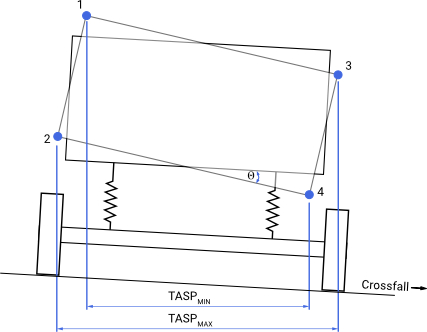
\includegraphics[width=0.7\textwidth]{fig/tasp_reference-point-height-influence}
	\caption{Influence of the reference point height on TASP performance}
	\label{figure:influence-of-reference-point-height-on-tasp}
\end{figure}
%----------------------------------------------
%      FIGURE
%----------------------------------------------

The \textbf{longitudinal standards} consisting of the \gls{sta}, \gls{graa}, \gls{grab} and \gls{acc} performance measures are highly influenced by the payload mass for the tridem interlink and rigid drawbar combination. For the quad semi-trailer, the trailer wheelbase is the most important variable for \gls{sta} and \gls{graa}.

When a heavy vehicle has a sufficiently powered engine, such as in the case of the three baseline combinations, the \gls{sta} and \gls{graa} are dependent on the traction force available at the drive tyres which is a function of the drive axle load when the coefficient of friction is kept constant (the NTC rules state a coefficient of friction of 0.8 should be used for the test road surfaces \cite{NationalTransportCommission2008}). Thus, the \gls{vdp} that has the most relative influence on the vehicle performance would be the one that provides the largest variation on the drive axle load.

The range within which the quad semi-trailer wheelbase was varied led to the wheelbase approaching the combined trailer and payload sprung mass centre of gravity location. At this point, most of the combined sprung mass was supported by the trailer axle group with little load transfer to the prime mover through the 5th wheel hitch. As discussed in Section \ref{section:pr-wheelbase} the legal axle load limits were not considered in determining the range of viable wheelbases as this would limit the allowable wheelbase range for the baseline vehicles and insight would be lost into the effect of changing the wheelbase for combinations that are volume rather than payload limited. For vehicle combinations that are payload limited, the wheelbase will have a smaller range of variation when considering legal axle load limits resulting in a reduced influence.

The \gls{acc} and \gls{graa} tests are performed on a road with a 0\degree{} to 1\degree{} grade respectively and as a result there is always sufficient traction at the drive axle tyres. The \gls{acc} and \gls{graa} performance is therefore limited by the engine power and gross combination mass. The \gls{vdp} providing the most variation in \gls{gcm} becomes the most influential and for all combinations this is the trailer payload. The tridem interlink is equally affected by both trailer payloads since they are identical in mass and were varied within the same range.

The study considered the payload to go from the unladen condition to the maximum laden condition since it is realistic for a combination to operate within that range. In practice, a combination would be optimised for a maximum payload and the payload would have a small envelope of variation. In this case, adjustments to the prime mover engine (which was beyond the scope of this study) and/or geometrical properties which result in a change in drive axle load would provide a larger relative influence.

The \textbf{longitudinal CG location (\gls{cgx})} of the payload has a larger relative influence than those of the prime mover and trailer chassis. The prime mover and trailer chassis \gls{cgx} locations were varied within a larger range (20\% and 30\% respectively) relative to the payload (between 9\% and 13\% depending on baseline combination). However, since the mass of the payload is significantly higher than the chassis in all cases, a change in the payload \gls{cgx} has a higher influence.

The \textbf{lateral CG location (\gls{cgy})} of the payloads (the prime mover and trailer chassis to a much lesser extent) have a medium to high relative influence on the high-speed performance of the combinations, in particular the \gls{srt} and the \gls{srtrrcu}. Therefore it is important to ensure that the \gls{cgy} location is accurately modelled (for payloads in particular) and emphasises that a shift in payload due to poor strapping will have a significant effect on the rollover stability of a vehicle combination. A shift in the \gls{cgy} location in the same direction as the roll motion of the sprung mass will amplify the roll. The additional roll motion will cause the rear reference points to be projected further outward affecting the \gls{tasp} (as discussed above) as well as the \gls{ts} performance of the vehicle.

The \textbf{vertical CG location (\gls{cgz})} of the payload has a high influence on the \gls{srt} and the \gls{srtrrcu} performance for all combinations. This is explained by the simple first-order estimate of \gls{srt} from Gillespie \cite{Gillespie1992} shown in Equation~\ref{eqn:first-order-srt-gillespie} which ignores the effects of deflection in the suspension. The \gls{cgz} has a direct and higher impact on the first-order estimate of \gls{srt} than axle track which is confirmed in the \gls{cv} matrices as the axle track (discussed below) has only a medium influence on \gls{srt} performance.

%----------------------------------------------
%      EQUATION
%----------------------------------------------
\begin{align}
	\label{eqn:first-order-srt-gillespie}
	SRT = \frac{t}{2h}
\end{align}

Where 

$t$ = Vehicle track width (mm)

$h$ = Vehicle CGz height (mm)

%----------------------------------------------
%      EQUATION
%----------------------------------------------

%      SUBSECTION
%----------------------------------------------
\subsection{Suspension and Tyre VDPs}\label{section:disc-relative-influence-suspension-tyre}

The \textbf{suspension and tyre \glspl{vdp}} have a low to negligible influence on the low-speed standards except for the steer axle track which has a relatively high impact on the \gls{fs} performance. The \gls{fs} performance of a combination is measured as the swing out of the front of the cab relative to the steer axle path inscribed on the ground at the outer edge of the steer tyre around a 90\degree{} turn \cite{NationalTransportCommission2008}. Considering that the cab dimensions remain constant, a wider steer axle track reduces the \gls{fs} and a narrower track width increases the \gls{fs} of the combination. Within the range of evaluated steer axle track widths, the axle track has a high influence on the \gls{fs} performance for all combinations.

The \textbf{trailer axle track} for the tridem interlink and rigid combination have a medium influence on the \gls{srt} performance while it has a low influence on the \gls{srt} performance of the quad semi-trailer. The minimum axle track for the trailer axle with 445/65 R22.5 single tyres is close to the maximum for the other baseline combinations. The roll stiffness of the quad semi-trailer is therefore still high even at the minimum axle track and therefore other parameters have a larger effect on the \gls{srt} performance of the vehicle, diminishing the relative effect of the trailer axle track for this combination.

The \textbf{drive axle auxiliary roll stiffness} has a larger relative influence on the performance of the rigid drawbar combination. The rigid drawbar combination has a pintle hitch which is a non roll-coupled hitch. Thus, roll effects are not transferred between the trailer and rigid unit. The rigid prime mover acts as a single unit and the dolly along with the trailer act as the rearward roll coupled unit which are connected with a roll-coupled hitch (5th wheel) allowing transfer of roll moments between the dolly and trailer. Decreasing the auxiliary roll stiffness on the rigid prime mover degrades the overall roll stiffness of the prime mover to a larger degree than the other combinations since it is not assisted by the roll stiffness of the trailers. The amplified roll experienced by the rigid prime mover results in degraded high-speed performance. This suggests that compared to a combination with roll-coupled hitch points, a combination with non roll-coupled hitch points will be affected by a greater degree when the auxiliary roll stiffness is adjusted on a single vehicle unit.

The \textbf{trailer axle auxiliary roll stiffness} has a medium relative influence on \gls{tasp} and low to negligible influence on all other performance measures for the quad semi-trailer. In the case of the tridem interlink and rigid combination, trailer axle auxiliary roll stiffness has a medium to high influence on \gls{srt}, \gls{ydc}, \gls{ra} and \gls{hsto} and the maximum effect on \gls{tasp}.

The greater influence of trailer axle auxiliary roll stiffness on the \gls{ra} of the tridem interlink (maximum influence) and rigid drawbar combination (high influence) relative to the quad semi-trailer (negligible influence) can be explained when considering the overall roll stiffness. The wider axle track and increased number of axles on the trailer unit of the quad semi-trailer results in the combination having a high overall roll stiffness even with a low auxiliary roll stiffness. The tridem interlink has the narrowest axle track which exacerbates the effect of decreasing the trailer auxiliary roll stiffness and results in the trailer axle auxiliary roll stiffness having the maximum influence on \gls{ra} for this combination.

The baseline vehicles have reference points at the top of the trailer structure which assumes that the outermost point on the right of the vehicle is at the top of the trailer structure. This is typical of tautliners with buckles and side-tippers with the widest point at the top of the bin. The outermost left reference point is located near to the ground on the bumper of the prime mover. If the rear reference points were lower to the ground (at the base of the trailer deck for example), the height differential between the left and right outer reference points would be decreased. This would decrease how far outwards the reference points are extended from each other for a given amount of roll (see Figure~\ref{figure:influence-of-reference-point-height-on-tasp}) and the influence of auxiliary roll stiffness (affecting the amount of roll the vehicle experiences) on the \gls{tasp} performance would hence be reduced.

The only \textbf{tyre \gls{vdp}} that has a significant effect on overall vehicle performance is the cornering stiffness which has a low to medium influence on the \gls{hsto} performance for all the baseline combinations. The cornering stiffness has higher relative effect on the quad semi-trailer and tridem interlink.

The range by which the \textbf{trailer tyre cornering stiffness} was varied matches the relative influence for each tyre with the 315/80 R22.5 tyres (tridem interlink) having an 80\% variation, the 445/65 R22.5 tyres (quad semi-trailer) having a 73\% variation and the 285/70 R19.5 tyres (rigid drawbar combination) having a 64\% variation. Taking this into consideration, the trailer lateral tyre force still has a relatively lower influence on \gls{hsto} for the rigid combination. Considering the isolated tyre \gls{cv} matrices in Section~\ref{section:cv-tyre} in Appendix~\ref{appendix:complete-cv-matrix}, the trailer lateral tyre force has the maximum influence on \gls{hsto} for all combinations. This highlights that the lower influence is due to the \gls{hsto} being affected by the drive auxiliary roll stiffness to a much higher degree, diminishing the relative influence of the trailer lateral tyre force in relation to the complete set of vehicle \glspl{vdp}.

The \textbf{steer tyre cornering stiffness} has a high relative influence on the \gls{ydc} performance of the tridem interlink and quad semi-trailer combinations. A change in tyre cornering stiffness directly affects the magnitude of the input disturbance for a given pulse steer input.

The steer tyre cornering stiffness has the maximum relative influence on the \gls{stfd} performance of the rigid combination while it has a negligible effect on the other baseline combinations where the prime mover wheelbase has the maximum influence. The wheelbase for the rigid prime mover were significantly longer than that of the tractor prime mover, resulting in less of an influence on the steer axle load. The NTC rules document \cite{NationalTransportCommission2008} does indicate that \gls{stfd} is typically only an issue for road trains with a tri-axle drive arrangement with a wide axle spread and is therefore not of concern for the baseline combinations considered in this study.

Tyre manufacturers do not make the lateral tyre force curves (from which tyre cornering stiffness is measured) for their tyres readily available and as a result, conservative lateral tyre curves are used for \gls{pbs} assessments in South Africa. This is in alignment with the NTC rules requirement that if generic tyres are used in the analysis, the cornering characteristics must be consistent with worst-case performing tyres of the same size to ensure that any tyre of the same size can be used \cite{NationalTransportCommission2008}. The tyre data used is from \gls{umtri} \cite{Fancher1981, Bogard1991} measurements in the early 1980s and 1990s. Using these conservative tyre curves negates any performance benefits that modern \glspl{hcv} tyres have due to advances made in their material and construction. Testing of newer tyre models to produce accurate lateral tyre curves would be of benefit to the transport industry as more productive combinations could achieve the required performance within the \gls{pbs} framework when tested with actual tyre curves.

%==============================================
%      SECTION
%==============================================
\section{VDPs with Negligible Influence on Overall Vehicle Performance}\label{section:vdps-with-negligible-influence-on-overall-performance}

The complete \gls{cv} matrices (see Tables~\ref{table:complete-cv-quad-semi-trailer}~to~\ref{table:complete-cv-rigid-combination} in Appendix~\ref{appendix:complete-cv-matrix}) contain all evaluated \glspl{vdp} and provide insight into which \glspl{vdp} have negligible influence on vehicle performance within the \gls{pbs} framework. A \gls{vdp} with a negligible relative influence on all of the baseline combinations analysed in this study would likely have negligible relative influence on all \glspl{hcv}. 

Inspecting the complete \gls{cv} matrices in Appendix~\ref{appendix:complete-cv-matrix}, the \glspl{vdp} listed below are seen to have a negligible effect on overall vehicle performance for all baseline combinations. With discretion, these \glspl{vdp} could be conservatively estimated without significantly influencing the vehicle performance, providing a realistic prediction of vehicle performance without the need to acquire exact data from \glspl{oem}.

\textbf{Inertial \glspl{vdp}:}
\begin{enumerate}
	\item Prime mover and dolly sprung mass \gls{cgz}
	\item Prime mover, trailer and dolly \gls{ixx}
\end{enumerate}

\textbf{Geometrical \glspl{vdp}:}

The geometrical reference points directly affect the low-speed and \gls{tasp} performance measures. In some vehicle configurations, the reference points of certain vehicle units have no influence on the low-speed performance measures. These cases are listed below in the context of the baseline configurations.

\begin{enumerate}
	\item Tridem interlink follower trailer front overhang
	\item Tridem interlink leader trailer rear overhang
	\item Rigid combination trailer front overhang
\end{enumerate}

\textbf{Suspension \glspl{vdp}:}
\begin{enumerate}
	\item Steer and drive axle unsprung mass
	\item Drive axle track width
	\item Axle centre height
	\item Steer and trailer roll centre height
	\item Axle roll and yaw inertia
	\item Axle wheel centre height
	\item Axle damper response
	\item Axle damper track width
	\item Axle jounce and rebound stops
	\item Axle spring response \footnote{The drive and trailer suspensions are all fitted with airbag springs. The auxiliary roll stiffness of air suspensions is a result of the rigid axle and trailing arm assemblies which work as a stabiliser bar. Steel suspension has auxiliary roll stiffness because of the twisting of the spring leaves as well as a stabiliser bar if present \cite{Fu2002}. The spring response would have a larger effect on vehicle performance if a steel suspension is used as it would influence the overall roll stiffness to a greater degree.}
	\item Axle spring track width
\end{enumerate}

\textbf{Tyre \glspl{vdp}:}
\begin{enumerate}
	\item Dual tyre spacing
	\item Steer and trailer effective rolling radius
	\item Drive tyre lag
	\item Steer and drive tyre vertical spring rate
	\item Unloaded radius
	\item Wheel spin inertia
\end{enumerate}

%==============================================
%      SECTION
%==============================================
\section{Limitations of the Methodology}\label{section:discussion-methodology-limitations}

%      SUBSECTION
%----------------------------------------------
\subsection{Simulated Manoeuvre Control Parameters}\label{section:discussion-limitations-control-parameters}

The control parameters for all of the manoeuvres were kept constant in this study. The lane change manoeuvre (evaluating \gls{ra} and \gls{hsto}) and pulse steer test (evaluating \gls{ydc}) both have control parameters that need to be adjusted to ensure that the vehicle is performing the \gls{pbs} manoeuvre within the required limits.

The lane change manoeuvre control parameter is the driver preview time \texttt{TPREV\_CONSTANT}. The driver model looks ahead at the target path by a distance determined by the current speed of the vehicle and the driver preview time, and adjusts the angle of the steering wheel to minimise the tracking error between the actual and target path over the preview time \cite{MechanicalSimulationHelpFileDriverControls2017}. A shorter preview time improves the vehicle tracking, but could lead to the vehicle becoming unstable while a longer preview time improves vehicle stability but results in a higher tracking error. For the ISO lane change manoeuvre, the vehicle is required to have a tracking error of no greater than 30~mm according to the NTC rules \cite{NationalTransportCommission2008}.

The control parameter for the pulse steer manoeuvre is the steering input gain \texttt{STEER\_SW\_GAIN}. The steering input for the \gls{trucksim} manoeuvre is normalised to unity, the steering input gain then needs to be set such that the lateral acceleration of the lead unit reaches approximately 0.2~g (a value of between 0.19~g and 0.21~g is deemed reasonable to ensure fair assessment of vehicle performance) \cite{MechanicalSimulationTechMemoPBS2017}. If the gain is set too high, the manoeuvre performed will be too harsh and result in poor \gls{ydc} performance which could lead to failing a safe combination. Conversely if it is set too low, the \gls{ydc} performance will be unfairly improved and could result in the passing of an unsafe combination.

In this study the \gls{ra} and the \gls{hsto} are influenced by the lack of controls to ensure the lateral tracking error is below 30~mm and the \gls{ydc} is influenced by not keeping the lateral acceleration of the steer axle and lead vehicle unit at 0.2~g.

%      SUBSECTION
%----------------------------------------------
\subsection{Selection of VDP Ranges}\label{section:discussion-limitations-range}

The coefficient of variation is sensitive to the range of values evaluated (see Section~\ref{chapter:parameter-range-selection}) for each \gls{vdp} as well as the design of the baseline vehicle which limits the results from being universally true. A range within which each \gls{vdp} could be varied was determined in Section~\ref{chapter:parameter-range-selection}. These ranges are sensitive to the baseline designs and need to be considered when interpreting the \gls{cv} matrix.

Some of the \gls{vdp} ranges were developed by considering studies conducted in the USA, Canada, and Australia. The relative influence of the \glspl{vdp} is influenced by these ranges, and as a result determining the actual variation in these parameters for the South African fleet would improve the applicability of the study to South Africa as well as eliminate any bias due to conservative ranges where a lack of data was available.

The baseline vehicles were designed to be at or near the legal axle load limits. This left little scope for adjusting the wheelbase, mass of any vehicle units or payloads and CG location of any of the mass \glspl{vdp} without causing an axle group to exceed the legal limit. If the legal axle load limits were considered, then valuable insight would have been lost into the effect of changing these parameters in volume limited payloads. Thus, some of the vehicle configurations with altered wheelbase, mass, or \gls{cg} locations of any of the masses are not legal vehicles.

Every effort has been made to consider a reasonable range for each vehicle design parameter to avoid biasing the influence of the \glspl{vdp}. Percentage differences from the baseline have been provided should the reader wish to evaluate the affect of changing a \gls{vdp} by a larger or lesser degree.
\chapter{Conclusions}\label{Conclusions} 

This study evaluated the relative effect of \glspl{vdp} on three of the most common \glspl{hcv}, a quad semi-trailer, tridem interlink and rigid drawbar combination. To prevent the relative influence of any \gls{vdp} being over or underestimated, a range within which each \gls{vdp} could be varied was determined by considering \gls{oem} data, legal restrictions, physical constraints and South African PBS assessment data. Evaluating the influence of each \gls{vdp} within these ranges adds insight into the limitations imposed by restrictions on the variation of a \gls{vdp} and expands on previous research conducted by Prem et al. \cite{Prem2002}.

The influence of a \gls{vdp} on vehicle performance for each \gls{pbs} performance measure was quantified with the coefficient of variation (\gls{cv}) metric. A comparative matrix (denoted as the \gls{cv} matrix) was developed for each baseline vehicle which compares the relative influence of each \gls{vdp} in terms of each of the \gls{pbs} performance measures. 

The overall \gls{cv} matrices (see Tables~\ref{table:overall-cv-quad-semi}~to~\ref{table:overall-cv-rigid}) provide insight into which \glspl{vdp} are the most influential in terms of each of the \gls{pbs} performance measures. If a proposed vehicle design fails a PBS assessment, the columns for each of the failed \gls{pbs} performance measures can be consulted to determine which \glspl{vdp} will yield the most improved performance for that \gls{pbs} performance measure.

The complete \gls{cv} matrices (see Tables~\ref{table:complete-cv-quad-semi-trailer}~to~\ref{section:complete-cv-rigid-drawbar}) highlight the \glspl{vdp} that have a negligible relative influence for all \gls{pbs} performance measures for all baseline combinations. A much larger proportion of suspension and tyre \glspl{vdp} were found to have a negligible relative influence compared to the inertial and geometric \gls{vdp}. These \glspl{vdp} (listed in Section~\ref{section:vdps-with-negligible-influence-on-overall-performance}) would likely have a negligible relative influence on all \glspl{hcv}. Using discretion, these \glspl{vdp} could be conservatively estimated and still provide realistic prediction of vehicle performance.

Additional \gls{cv} matrices were developed comparing the inertial, geometrical, suspension and tyre \glspl{vdp} in isolation (see Appendices~\ref{section:cv-geometrical}~to~\ref{section:cv-tyre}). These \gls{cv} matrices highlight the \glspl{vdp} with the most influence within each category independent of all other \glspl{vdp} and will guide efforts focussed on a specific area of vehicle design.
 
The results contained in this study will help speed up the \gls{pbs} assessment process and guide vehicle design efforts towards high-impact \glspl{vdp} when optimising vehicle design leading to safer, more productive \glspl{hcv}.

%----------------------------------------------
%      PRINT BIBLIOGRAPHY
%----------------------------------------------
\sloppy
% The references section set-up as below will allow for it to be references in the text and ensure that the heading is references instead of bibliography
\chapter*{References}\label{section:references}
\addcontentsline{toc}{chapter}{References}
\printbibliography[heading=none]
\fussy

%----------------------------------------------
%      Glossary - removed for now
%----------------------------------------------
% \glossarylist{} 

%----------------------------------------------
%      Appendices
%----------------------------------------------
\appendix %Command which changes the formatting of subsequent sections to be appendices
\chapter{Baseline Vehicle Model Data}\label{appendix:baseline-models}

%----------------------------------------------
%      SECTION
%----------------------------------------------
\section{Summary of Baseline Vehicle Design Parameters}\label{section:summary-of-evaluted-vehicle-design-parameters}

The sections that follow summarise the configuration of each baseline combination and include the range of values evaluated for each \gls{vdp}. The ranges have been separated into the following categories; vehicle units (prime movers and trailers), axles and tyres.

%      SUBSECTION
%----------------------------------------------
\subsection{Vehicle Design Parameters for Vehicle Units}\label{section:summary-of-vehicle-unit-design-parameters}

%      SUBSUBSECTION --------------------------
\subsubsection{Prime Movers}\label{section:vdp-range-prime-mover}

The axle configuration on the truck tractor and rigid truck is as follows:

\begin{enumerate}
	\item \textbf{Steer:} Steer axle with 315/80 R22.5 tyres (see Table~\ref{table:vdp-range-axle-steer-315})
	\item \textbf{Drive:} Drive axle with 315/80 R22.5 tyres (see Table~\ref{table:vdp-range-axle-drive-315})
\end{enumerate}

A detailed summary of the \glspl{vdp} and their evaluated range for the truck tractor and rigid truck is presented in Tables~\ref{table:vdp-range-prime-mover-tractor} and \ref{table:vdp-range-prime-mover-rigid} respectively.

Both baseline prime movers are fitted with the same engine, gearbox and powertrain as per Tables~\ref{table:baseline-engine-torque-curve}~to~\ref{table:baseline-differential} which remain unchanged for all simulations.

%----------------------------------------------
%      TABLE
%----------------------------------------------
\begin{table}[H]
	\centering\footnotesize
	\begin{threeparttable}

		\begin{tabulary}{\textwidth}{lcccccc}
			\toprule
			\textbf{Parameter} & \textbf{Unit} & \textbf{Baseline} & \textbf{Min.} & \textbf{Max.} & \textbf{Min. (\%)} & \textbf{Max. (\%)} \\

			\midrule
			Wheelbase & mm    & 3885  & 3061  & 4360  & 79\%  & 112\% \\
			Axle spacing & mm    & 1370  & 1200  & 1400  & 88\%  & 102\% \\
			Hitch height & mm    & 1278  & 1088  & 1350  & 85\%  & 106\% \\
			Hitch longitudinal location & mm    & -3375  & -3200  & -3885  & 95\%  & 115\% \\
			Prime mover sprung mass & kg    & 6598  & 4428  & 6598  & 67\%  & 100\% \\
			Prime mover \gls{cgx} & mm    & -1001  & -801   & -1201  & 80\%  & 120\% \\
			Prime mover \gls{cgy} & mm    & 0     & -250   & 250   & 10\% of width & 10\% of width \\
			Prime mover \gls{cgz} & mm    & 1204  & 1070  & 1426  & 89\%  & 118\% \\
			Prime mover \gls{rx} & m     & 0.760 & 0.532 & 0.988 & 70\%  & 130\% \\
			Prime mover \gls{ry} & m     & 1.943 & 1.166 & 2.720 & 60\%  & 140\% \\
			Prime mover \gls{rz} & m     & 1.943 & 1.166 & 2.720 & 60\%  & 140\% \\
			Front overhang & mm    & 1365  & 1300  & 1820  & 95\%  & 133\% \\
			Rear overhang & mm    & 1013  & 1013  & 1013  & Not varied & Not varied \\
			Vehicle width cab & mm    & 2495  & 2225  & 2600  & 89\%  & 104\% \\
			Reference point height & mm    & 752   & 0     & 4600  & 0\%   & 612\% \\

			\bottomrule
		\end{tabulary}

		\caption{Vehicle design parameters - truck tractor}
		\label{table:vdp-range-prime-mover-tractor}

% 				\begin{tablenotes}
%         		\item[1]SAE up co-ordinate system and origin taken from centre of steer axle at ground level
% 				\item[2] Measured from the centre of the rearmost axle in accordance with Regulation 226 (2)(c)
% 				\end{tablenotes}

	\end{threeparttable}
\end{table}
%----------------------------------------------
%      TABLE
%----------------------------------------------

%----------------------------------------------
%      TABLE
%----------------------------------------------
\begin{table}[H]
	\centering\footnotesize
	\begin{threeparttable}

		\begin{tabulary}{\textwidth}{lcccccc}
			\toprule
			\textbf{Parameter} & \textbf{Unit} & \textbf{Baseline} & \textbf{Min.} & \textbf{Max.} & \textbf{Min. (\%)} & \textbf{Max. (\%)} \\

			\midrule
			Wheelbase & mm    & 5285  & 4413  & 5892  & 84\%  & 111\% \\
			\multicolumn{1}{l}{Axle spacing} & mm    & 1370  & 1200  & 1400  & 88\%  & 102\% \\
			Hitch height & mm    & 500   & 300   & 918   & 60\%  & 184\% \\
			Hitch longitudinal location & mm    & -7115  & -6558  & -7860  & 92\%  & 110\% \\
			Prime mover sprung mass & kg    & 6698  & 4767  & 6698  & 71\%  & 100\% \\
			Prime mover \gls{cgx} & mm    & -1860  & -1488  & -2232  & 80\%  & 120\% \\
			Prime mover \gls{cgy} & mm    & 0     & -260  & 260   & 10\% of width & 10\% of width \\
			Prime mover \gls{cgz} & mm    & 1017  & 1000  & 1315  & 98\%  & 129\% \\
			Prime mover \gls{rx} & m     & 0.76  & 0.532 & 0.988 & 70\%  & 130\% \\
			Prime mover \gls{ry} & m     & 2.643 & 1.586 & 3.700 & 60\%  & 140\% \\
			Prime mover \gls{rz} & m     & 2.643 & 1.586 & 3.700 & 60\%  & 140\% \\
			Front overhang & mm    & 1365  & 1300  & 1820  & 95\%  & 133\% \\
			Rear overhang & mm    & 1775  & 0     & 2546  & 0\%   & 143\% \\
			Vehicle width (superstructure) & mm    & 2600  & 2400  & 2600  & 92\%  & 100\% \\
			Vehicle width (cab) & mm    & 2495  & 2225  & 2600  & 89\%  & 104\% \\
			Reference point height & mm    & 752   & 0     & 4600  & 0\%   & 612\% \\
			Payload sprung mass & kg    & 15352 & 0     & 15352 & 0\%   & 100\% \\
			Payload \gls{cgx} & mm    & -4490  & -4176  & -4804  & 93\%  & 107\% \\
			Payload \gls{cgy} & mm    & 0     & -260  & 260   & 10\% of width & 10\% of width \\
			Payload \gls{cgz} & mm    & 2504  & 1122  & 2968  & 45\%  & 119\% \\
			Payload \gls{rx} & m     & 1.488 & 0.744 & 2.232 & 50\%  & 150\% \\
			Payload \gls{ry} & m     & 1.839 & 0.736 & 2.942 & 40\%  & 160\% \\
			Payload \gls{rz} & m     & 1.860 & 0.744 & 2.976 & 40\%  & 160\% \\

			\bottomrule
		\end{tabulary}

		\caption{Vehicle design parameters - rigid truck}
		\label{table:vdp-range-prime-mover-rigid}

		%\begin{tablenotes}
		%\item[1] %\tnote{1}
		%\end{tablenotes}

	\end{threeparttable}
\end{table}
%----------------------------------------------
%      TABLE
%----------------------------------------------

%----------------------------------------------
%      TABLE
%----------------------------------------------
\begin{table}[H]
	\centering\footnotesize
	\begin{threeparttable}

		\begin{tabulary}{\textwidth}{cc}
			\toprule
			Engine speed (rpm) & Torque (Nm)\\
			\midrule
			600   & 1273 \\
			621   & 1305 \\
			688   & 1404 \\
			749   & 1499 \\
			810   & 1601 \\
			856   & 1704 \\
			901   & 1803 \\
			929   & 1893 \\
			965   & 1996 \\
			996   & 2099 \\
			1053  & 2201 \\
			1394  & 2205 \\
			1461  & 2095 \\
			1540  & 1996 \\
			1631  & 1897 \\
			1714  & 1803 \\
			1811  & 1700 \\
			1860  & 1601 \\
			1911  & 1499 \\
			1951  & 1404 \\
			1997  & 1301 \\
			2033  & 1203 \\
			2085  & 1100 \\
			\bottomrule
		\end{tabulary}

		\caption{Baseline engine torque curve}
		\label{table:baseline-engine-torque-curve}

		%\begin{tablenotes}
		%\item[1] %\tnote{1}
		%\end{tablenotes}

	\end{threeparttable}
\end{table}
%----------------------------------------------
%      TABLE
%----------------------------------------------

%----------------------------------------------
%      TABLE
%----------------------------------------------
\begin{table}[H]
	\centering\footnotesize
	\begin{threeparttable}

		\begin{tabulary}{\textwidth}{ccc}
			\toprule
			Gear & Ratio & Efficiencies\\
			\midrule
			C     & 19.38 & 0.96 \\
			1     & 14.94 & 0.96 \\
			2     & 11.28 & 0.96 \\
			3     & 9.04  & 0.96 \\
			4     & 7.09  & 0.96 \\
			5     & 5.54  & 0.96 \\
			6     & 4.35  & 0.96 \\
			7     & 3.44  & 0.96 \\
			8     & 2.7   & 0.96 \\
			9     & 2.08  & 0.96 \\
			10    & 1.63  & 0.96 \\
			11    & 1.27  & 0.96 \\
			12    & 1     & 0.96 \\
			\bottomrule
		\end{tabulary}

		\caption{Baseline gearbox transmission data}
		\label{table:baseline-gearbox-transmission-data}

		%\begin{tablenotes}
		%\item[1] %\tnote{1}
		%\end{tablenotes}

	\end{threeparttable}
\end{table}
%----------------------------------------------
%      TABLE
%----------------------------------------------

%----------------------------------------------
%      TABLE
%----------------------------------------------
\begin{table}[H]
	\centering\footnotesize
	\begin{threeparttable}

		\begin{tabulary}{\textwidth}{CCCCC}
			\toprule
			Differential ratio & Differential efficiency & Clutch engagement speed (rpm) & Clutch engagement torque (Nm) & Gear change speed (rpm)\\
			\midrule
			3.09  & 0.98  & 600   & 1103  & 1631 \\
			\bottomrule
		\end{tabulary}

		\caption{Baseline differential, clutch engagement and gear change speed}
		\label{table:baseline-differential}

		%\begin{tablenotes}
		%\item[1] %\tnote{1}
		%\end{tablenotes}

	\end{threeparttable}
\end{table}
%----------------------------------------------
%      TABLE
%----------------------------------------------



\subsubsection{Trailer and Dolly Units}\label{section:vdp-range-trailers}

The axle configuration on the \textbf{quad semi-trailer} is as follows:

\begin{enumerate}
	\item \textbf{Trailer:} Trailer axle with 445/65 R22.5 tyres (see Table~\ref{table:vdp-range-axle-trailer-445}).
\end{enumerate}

A detailed summary of the \glspl{vdp} and their evaluated range for the quad semi-trailer is presented in Table~\ref{table:vdp-range-trailer-quad-semi}.

%----------------------------------------------
%      TABLE
%----------------------------------------------
\begin{table}[H]
	\centering\footnotesize
	\begin{threeparttable}

		\begin{tabulary}{\textwidth}{lcccccc}
			\toprule
			\textbf{Parameter} & \textbf{Unit} & \textbf{Baseline} & \textbf{Min.} & \textbf{Max.} & \textbf{Min. (\%)} & \textbf{Max. (\%)} \\

			\midrule
			Wheelbase & mm    & 10000 & 7975  & 10000 & 80\%  & 100\% \\
			Axle spacing & mm    & 1360  & 1200  & 1850  & 88\%  & 136\% \\
			Trailer sprung mass & kg    & 10410 & 2500  & 10410 & 24\%  & 100\% \\
			Trailer \gls{cgx} & mm    & -6455  & -4519  & -8392  & 70\%  & 130\% \\
			Trailer \gls{cgy} & mm    & 0     & -260  & 260   & 10\% of width & 10\% of width \\
			Trailer \gls{cgz} & mm    & 2025  & 1280  & 2025  & 63\%  & 100\% \\
			Trailer \gls{rx} & m     & 1.588 & 0.873 & 2.303 & 55\%  & 145\% \\
			Trailer \gls{ry} & m     & 4.641 & 2.321 & 6.962 & 50\%  & 150\% \\
			Trailer \gls{rz} & m     & 4.685 & 2.343 & 7.028 & 50\%  & 150\% \\
			Front overhang & mm & 900   & 0     & 1800  & 0\%   & 200\% \\
			Rear overhang & mm & 1960  & 0     & 6000  & 0\%   & 306\% \\
			Vehicle width & mm    & 2600  & 2400  & 2600  & 92\%  & 100\% \\
			Reference point height & mm & 3800  & 0     & 4600  & 0\%   & 121\% \\
			Payload sprung mass & kg    & 32000 & 0     & 32000 & 0\%   & 100\% \\
			Payload \gls{cgx} & mm    & -6500  & -5755  & -7245  & 89\%  & 111\% \\
			Payload \gls{cgy} & mm    & 0     & -260  & 260   & 10\% of width & 10\% of width \\
			Payload \gls{cgz} & mm    & 2025  & 1580  & 2841  & 78\%  & 140\% \\
			Payload \gls{rx} & m     & 0.812 & 0.406 & 1.218 & 50\%  & 150\% \\
			Payload \gls{ry} & m     & 4.368 & 1.747 & 6.989 & 40\%  & 160\% \\
			Payload \gls{rz} & m     & 4.353 & 1.741 & 6.965 & 40\%  & 160\% \\

			\bottomrule
		\end{tabulary}

		\caption{Vehicle design parameters - quad semi-trailer}
		\label{table:vdp-range-trailer-quad-semi}

		%\begin{tablenotes}
		%\item[1] %\tnote{1}
		%\end{tablenotes}

	\end{threeparttable}
\end{table}
%----------------------------------------------
%      TABLE
%----------------------------------------------
\newpage
The axle configuration on the \textbf{tridem interlink leader and follower trailers} is as follows:

\begin{enumerate}
	\item \textbf{Trailer:} Trailer axle with 315/80 R22.5 tyres (see Table~\ref{table:vdp-range-axle-trailer-315})
\end{enumerate}

A detailed summary of the \glspl{vdp} and their evaluated range for the tridem interlink leader and follower trailer is presented in Tables~\ref{table:vdp-range-trailer-tridem-interlink-leader}~and~\ref{table:vdp-range-trailer-tridem-interlink-follower} respectively.

%----------------------------------------------
%      TABLE
%----------------------------------------------
\begin{table}[H]
	\centering\footnotesize
	\begin{threeparttable}

		\begin{tabulary}{\textwidth}{lcccccc}
			\toprule
			\textbf{Parameter} & \textbf{Unit} & \textbf{Baseline} & \textbf{Min.} & \textbf{Max.} & \textbf{Min. (\%)} & \textbf{Max. (\%)} \\

			\midrule
			Wheelbase & mm & 7420  & 7060  & 7612  & 95\%  & 103\% \\
			Axle spacing & mm    & 1360  & 1200  & 1850  & 88\%  & 136\% \\
			Hitch height & mm    & 1278  & 1148  & 1350  & 90\%  & 106\% \\
			Hitch longitudinal location & mm    & -8420  & -7925  & -8780  & 94\%  & 104\% \\
			Trailer sprung mass & kg    & 4632  & 1855  & 4632  & 40\%  & 100\% \\
			Trailer \gls{cgx} & mm    & -3656  & -2559  & -4753  & 70\%  & 130\% \\
			Trailer \gls{cgy} & mm    & 0     & -260  & 260   & 10\% of width & 10\% of width \\
			Trailer \gls{cgz} & mm    & 1777  & 1280  & 2025  & 72\%  & 114\% \\
			Trailer \gls{rx} & m     & 0.985 & 0.542 & 1.428 & 55\%  & 145\% \\
			Trailer \gls{ry} & m     & 3.169 & 1.585 & 4.754 & 50\%  & 150\% \\
			Trailer \gls{rz} & m     & 3.167 & 1.584 & 4.751 & 50\%  & 150\% \\
			Front overhang & mm & 950   & 0     & 1800  & 0\%   & 189\% \\
			Rear overhang & mm & -1790 & -1790 & -1283 & 100\% & 72\% \\
			Vehicle width & mm    & 2600  & 2400  & 2600  & 92\%  & 100\% \\
			Reference point height & mm    & 3198  & 0     & 4600  & 0\%   & 144\% \\
			Payload sprung mass & kg    & 24615 & 0     & 24615 & 0\%   & 100\% \\
			Payload \gls{cgx} & mm    & -3111  & -2714  & -3508  & 87\%  & 113\% \\
			Payload \gls{cgy} & mm    & 0     & -260  & 260   & 10\% of width & 10\% of width \\
			Payload \gls{cgz} & mm    & 2375  & 1667  & 2473  & 70\%  & 104\% \\
			Payload \gls{rx} & m     & 0.762 & 0.381 & 1.143 & 50\%  & 150\% \\
			Payload \gls{ry} & m     & 2.211 & 0.884 & 3.538 & 40\%  & 160\% \\
			Payload \gls{rz} & m     & 2.251 & 0.900 & 3.602 & 40\%  & 160\% \\

			\bottomrule
		\end{tabulary}

		\caption{Vehicle design parameters - tridem interlink leader}
		\label{table:vdp-range-trailer-tridem-interlink-leader}

		%\begin{tablenotes}
		%\item[1] %\tnote{1}
		%\end{tablenotes}

	\end{threeparttable}
\end{table}
%----------------------------------------------
%      TABLE
%----------------------------------------------

%----------------------------------------------
%      TABLE
%----------------------------------------------
\begin{table}[H]
	\centering\footnotesize
	\begin{threeparttable}

		\begin{tabulary}{\textwidth}{lcccccc}
			\toprule
			\textbf{Parameter} & \textbf{Unit} & \textbf{Baseline} & \textbf{Min.} & \textbf{Max.} & \textbf{Min. (\%)} & \textbf{Max. (\%)} \\

			\midrule
			Wheelbase & mm & 5950  & 4434  & 6404  & 75\%  & 108\% \\
			Axle spacing & mm    & 1360  & 1200  & 1850  & 88\%  & 136\% \\
			Trailer sprung mass & kg    & 4167  & 1488  & 4167  & 36\%  & 100\% \\
			Trailer \gls{cgx} & mm    & -4269  & -2988  & -5550  & 70\%  & 130\% \\
			Trailer \gls{cgy} & mm    & 0     & -260  & 260   & 10\% of width & 10\% of width \\
			Trailer \gls{cgz} & mm    & 1912  & 1280  & 2025  & 67\%  & 106\% \\
			Trailer \gls{rx} & m     & 1.007 & 0.554 & 1.460 & 55\%  & 145\% \\
			Trailer \gls{ry} & m     & 3.037 & 1.519 & 4.556 & 50\%  & 150\% \\
			Trailer \gls{rz} & m     & 3.052 & 1.526 & 4.578 & 50\%  & 150\% \\
			Front overhang & mm & -354  & -354  & 464   & 100\% & -131\% \\
			Rear overhang & mm & 984   & 0     & 3570  & 0\%   & 363\% \\
			Vehicle width & mm    & 2600  & 2400  & 2600  & 92\%  & 100\% \\
			Reference point height & mm    & 4114  & 0     & 4600  & 0\%   & 112\% \\
			Payload sprung mass & kg    & 24615 & 0     & 24615 & 0\%   & 100\% \\
			Payload \gls{cgx} & mm    & -4403  & -4006  & -4800  & 91\%  & 109\% \\
			Payload \gls{cgy} & mm    & 0     & -260  & 260   & 10\% of width & 10\% of width \\
			Payload \gls{cgz} & mm    & 2375  & 1667  & 2473  & 70\%  & 104\% \\
			Payload \gls{rx} & m     & 0.762 & 0.381 & 1.143 & 50\%  & 150\% \\
			Payload \gls{ry} & m     & 2.211 & 0.884 & 3.538 & 40\%  & 160\% \\
			Payload \gls{rz} & m     & 2.251 & 0.900 & 3.602 & 40\%  & 160\% \\

			\bottomrule
		\end{tabulary}

		\caption{Vehicle design parameters - tridem interlink follower}
		\label{table:vdp-range-trailer-tridem-interlink-follower}

		%\begin{tablenotes}
		%\item[1] %\tnote{1}
		%\end{tablenotes}

	\end{threeparttable}
\end{table}
%----------------------------------------------
%      TABLE
%----------------------------------------------
\newpage
The axle configuration on the \textbf{rigid drawbar combination} is as follows:

\begin{enumerate}
	\item \textbf{Dolly:} Trailer axle with 285/70 R19.5 tyres (see Table~\ref{table:vdp-range-axle-trailer-285})
	\item \textbf{Trailer:} Trailer axle with 285/70 R19.5 tyres (see Table~\ref{table:vdp-range-axle-trailer-285})
\end{enumerate}

A detailed summary of the \glspl{vdp} and their evaluated range for the rigid drawbar combination tridem semi-trailer and dolly is presented in Tables~\ref{table:vdp-range-trailer-rigid-combination-trailer}~and~\ref{table:vdp-range-trailer-rigid-combination-dolly} respectively.

%----------------------------------------------
%      TABLE
%----------------------------------------------
\begin{table}[H]
	\centering\footnotesize
	\begin{threeparttable}

		\begin{tabulary}{\textwidth}{lcccccc}
			\toprule
			\textbf{Parameter} & \textbf{Unit} & \textbf{Baseline} & \textbf{Min.} & \textbf{Max.} & \textbf{Min. (\%)} & \textbf{Max. (\%)} \\

			\midrule
			Wheelbase & mm & 8255  & 6035  & 8881  & 73\%  & 108\% \\
			Axle spacing & mm    & 1360  & 1200  & 1850  & 88\%  & 136\% \\
			Trailer sprung mass & kg    & 3150  & 2064  & 3150  & 66\%  & 100\% \\
			Trailer \gls{cgx} & mm    & -5575  & -3903  & -7248  & 70\%  & 130\% \\
			Trailer \gls{cgy} & mm    & 0     & -260  & 260   & 10\% of width & 10\% of width \\
			Trailer \gls{cgz} & mm    & 1500  & 1280  & 2025  & 85\%  & 135\% \\
			Trailer \gls{rx} & m     & 1.227 & 0.675 & 1.779 & 55\%  & 145\% \\
			Trailer \gls{ry} & m     & 5.434 & 2.717 & 8.151 & 50\%  & 150\% \\
			Trailer \gls{rz} & m     & 5.501 & 2.751 & 8.252 & 50\%  & 150\% \\
			Front overhang & mm & 1760  & 0     & 1800  & 0\%   & 102\% \\
			Rear overhang & mm & 1081  & 0     & 4953  & 0\%   & 458\% \\
			Vehicle width & mm    & 2600  & 2400  & 2600  & 92\%  & 100\% \\
			Reference point height & mm    & 3198  & 0     & 4600  & 0\%   & 144\% \\
			Payload sprung mass & kg    & 34000 & 0     & 34000 & 0\%   & 100\% \\
			Payload \gls{cgx} & mm    & -4702  & -4079  & -5325  & 87\%  & 113\% \\
			Payload \gls{cgy} & mm    & 0     & -260  & 260   & 10\% of width & 10\% of width \\
			Payload \gls{cgz} & mm    & 2575  & 1371  & 3012  & 53\%  & 117\% \\
			Payload \gls{rx} & m     & 1.506 & 0.753 & 2.259 & 50\%  & 150\% \\
			Payload \gls{ry} & m     & 3.656 & 1.462 & 5.850 & 40\%  & 160\% \\
			Payload \gls{rz} & m     & 3.656 & 1.462 & 5.850 & 40\%  & 160\% \\

			\bottomrule
		\end{tabulary}

		\caption{Vehicle design parameters - tridem semi-trailer}
		\label{table:vdp-range-trailer-rigid-combination-trailer}

		%\begin{tablenotes}
		%\item[1] %\tnote{1}
		%\end{tablenotes}

	\end{threeparttable}
\end{table}
%----------------------------------------------
%      TABLE
%----------------------------------------------

%----------------------------------------------
%      TABLE
%----------------------------------------------
\begin{table}[H]
	\centering\footnotesize
	\begin{threeparttable}

		\begin{tabulary}{\textwidth}{lcccccc}
			\toprule
			\textbf{Parameter} & \textbf{Unit} & \textbf{Baseline} & \textbf{Min.} & \textbf{Max.} & \textbf{Min. (\%)} & \textbf{Max. (\%)} \\

			\midrule
			Wheelbase & mm    & 3590  & 2819  & 4841  & 79\%  & 135\% \\
			Axle spacing & mm    & 1360  & 1200  & 1800  & 88\%  & 132\% \\
			Hitch height & mm    & 1100  & 970   & 1350  & 88\%  & 123\% \\
			Hitch longitudinal location & mm    & -3639  & -3385  & -3785  & 93\%  & 104\% \\
			Dolly sprung mass & kg    & 453   & 400   & 453   & 88\%  & 100\% \\
			Dolly \gls{cgx} & mm    & -3450  & -3105  & -3795  & 90\%  & 110\% \\
			Dolly \gls{cgy} & mm    & 0     & 0     & 0     & Not varied & Not varied \\
			Dolly \gls{cgz} & mm    & 868   & 868   & 1050  & 100\% & 121\% \\
			Dolly \gls{rx} & m     & 0.515 & 0.412 & 0.618 & 80\%  & 120\% \\
			Dolly \gls{ry} & m     & 0.818 & 0.573 & 1.063 & 70\%  & 130\% \\
			Dolly \gls{rz} & m     & 0.959 & 0.671 & 1.247 & 70\%  & 130\% \\

			\bottomrule
		\end{tabulary}

		\caption{Vehicle design parameters - rigid combination dolly}
		\label{table:vdp-range-trailer-rigid-combination-dolly}

		%\begin{tablenotes}
		%\item[1] %\tnote{1}
		%\end{tablenotes}

	\end{threeparttable}
\end{table}
%----------------------------------------------
%      TABLE
%----------------------------------------------

%      SUBSECTION
%----------------------------------------------
\subsection{Vehicle Design Parameters for Axles}\label{section:summary-of-axle-design-parameters}

Tables~\ref{table:vdp-range-axle-steer-315}~to~\ref{table:vdp-range-axle-trailer-285} summarise the \glspl{vdp} for the baseline axles.

%----------------------------------------------
%      TABLE
%----------------------------------------------
\begin{table}[H]
	\centering\footnotesize
	\begin{threeparttable}

		\begin{tabulary}{\textwidth}{lcccccc}
			\toprule
			\textbf{Parameter} & \textbf{Unit} & \textbf{Baseline} & \textbf{Min.} & \textbf{Max.} & \textbf{Min. (\%)} & \textbf{Max. (\%)} \\

			\midrule
			Axle track & mm    & 2109  & 1950  & 2282  & 92\%  & 108\% \\
			Axle centre height & mm    & 507   & 447   & 567   & 88\%  & 112\% \\
			Roll centre height & mm    & 21    & -20   & 100   & -95\% & 476\% \\
			Roll steer coefficient & \degree{}/\degree{} & -0.087 & 0     & -0.2  & 0\%   & 230\% \\
			Axle \gls{ixx}/\gls{izz}  & kg.m\sstw{} & 529   & 529   & 621   & 100\% & 117\% \\
			Spin inertia for each side & kg.m\sstw{} & 2     & 2     & 20    & 100\% & 1000\% \\
			Unsprung mass  & kg    & 750   & 544   & 800   & 67\%  & 107\% \\
			Wheel centre height & mm    & 507   & 507   & 528   & 100\% & 104\% \\
			Auxiliary roll stiffness  & Nm/\degree{} & 2950  & 1070  & 5009  & 36\%  & 170\% \\
			Damper model & N-s/mm & 20    & 2.5   & 50    & 13\%  & 250\% \\
			Damper track & mm    & 1150  & 780   & 1150  & 68\%  & 100\% \\
			Jounce stop & mm    & 204   & 45    & 250   & 22\%  & 123\% \\
			Rebound stop & mm    & -195  & -45   & -250  & 23\%  & 128\% \\
			Spring vertical stiffness & N/mm  & 273   & 185   & 350   & 68\%  & 128\% \\
			Spring track & mm    & 815   & 780   & 1150  & 96\%  & 141\% \\

			\bottomrule
		\end{tabulary}

		\caption{Vehicle design parameters - steer axle with 315/80 R22.5 tyres (singles)}
		\label{table:vdp-range-axle-steer-315}

		%\begin{tablenotes}
		%\item[1] %\tnote{1}
		%\end{tablenotes}

	\end{threeparttable}
\end{table}
%----------------------------------------------
%      TABLE
%----------------------------------------------

%----------------------------------------------
%      TABLE
%----------------------------------------------
\begin{table}[H]
	\centering\footnotesize
	\begin{threeparttable}

		\begin{tabulary}{\textwidth}{lcccccc}

			\toprule
			\textbf{Parameter} & \textbf{Unit} & \textbf{Baseline} & \textbf{Min.} & \textbf{Max.} & \textbf{Min. (\%)} & \textbf{Max. (\%)} \\

			\midrule
			Axle track & mm    & 1837  & 1800  & 1932  & 98\%  & 105\% \\
			Axle centre height & mm    & 507   & 447   & 567   & 88\%  & 112\% \\
			Roll centre height & mm    & 400   & -125  & 400   & -31\% & 100\% \\
			Roll steer coefficient & \degree{}/\degree{} & 0     & 0.04  & -0.23 & -     & - \\
			Axle \gls{ixx}/\gls{izz}  & kg.m\sstw{} & 619   & 619   & 712   & 100\% & 115\% \\
			Spin inertia for each side & kg.m\sstw{} & 2     & 2     & 20    & 100\% & 1000\% \\
			Unsprung mass  & kg    & 1300  & 1043   & 1350  & 69\%  & 104\% \\
			Wheel centre height & mm    & 507   & 507   & 528   & 100\% & 104\% \\
			Auxiliary roll stiffness  & Nm/\degree{} & 7487  & 790   & 12689 & 11\%  & 169\% \\
			Damper model & N-s/mm & 20    & 2.5   & 50    & 13\%  & 250\% \\
			Damper track & mm    & 1000  & 670   & 1100  & 67\%  & 110\% \\
			Jounce stop & mm    & 250   & 45    & 250   & 18\%  & 100\% \\
			Rebound stop & mm    & -250  & -45   & -250  & 18\%  & 100\% \\
			Spring vertical stiffness & \%\tnote{1}  & 100\% & 42\%  & 126\% & 42\%  & 126\% \\
			Spring track & mm    & 755   & 670   & 1100  & 89\%  & 146\% \\

			\bottomrule

		\end{tabulary}

		\caption{Vehicle design parameters - drive axle with 315/80 R22.5 tyres (duals)}
		\label{table:vdp-range-axle-drive-315}

		\begin{tablenotes}
			\item[1] Spring vertical stiffness response scaled as a percentage of the baseline spring response
		\end{tablenotes}

	\end{threeparttable}
\end{table}
%----------------------------------------------
%      TABLE
%----------------------------------------------

%----------------------------------------------
%      TABLE
%----------------------------------------------
\begin{table}[H]
	\centering\footnotesize
	\begin{threeparttable}

		\begin{tabulary}{\textwidth}{lcccccc}
			\toprule
			\textbf{Parameter} & \textbf{Unit} & \textbf{Baseline} & \textbf{Min.} & \textbf{Max.} & \textbf{Min. (\%)} & \textbf{Max. (\%)} \\

			\midrule
			Axle track & mm    & 2140  & 2000  & 2178  & 93\%  & 102\% \\
			Axle centre height & mm    & 534   & 474   & 594   & 89\%  & 111\% \\
			Roll centre height & mm    & 114   & -125  & 200   & -110\% & 175\% \\
			Roll steer coefficient & \degree{}/\degree{} & -0.035 & 0.04  & -0.23 & -114\% & 657\% \\
			Axle \gls{ixx}/\gls{izz}  & kg.m\sstw{} & 474   & 474   & 562   & 100\% & 119\% \\
			Spin inertia for each side & kg.m\sstw{} & 2     & 2     & 20    & 100\% & 1000\% \\
			Unsprung mass  & kg    & 760   & 545   & 800   & 71\%  & 125\% \\
			Wheel centre height & mm    & 534   & 534   & 561   & 100\% & 105\% \\
			Auxiliary roll stiffness  & Nm/\degree{} & 24700 & 2260  & 35954 & 9\%   & 146\% \\
			Damper model & N-s/mm & 20    & 2.5   & 50    & 13\%  & 250\% \\
			Damper track & mm    & 1080  & 780   & 1500  & 72\%  & 139\% \\
			Jounce stop & mm    & 250   & 45    & 250   & 18\%  & 100\% \\
			Rebound stop & mm    & -250  & -45   & -250  & 18\%  & 100\% \\
			Spring vertical stiffness & \%\tnote{1}  & 100\% & 62\%  & 186\% & 62\%  & 186\% \\
			Spring track & mm    & 1300  & 780   & 1500  & 60\%  & 115\% \\

			\bottomrule
		\end{tabulary}

		\caption{Vehicle design parameters - trailer axle with 445/65 R22.5 tyres (singles)}
		\label{table:vdp-range-axle-trailer-445}

		\begin{tablenotes}
			\item[1] Spring vertical stiffness response scaled as a percentage of the baseline spring response
		\end{tablenotes}

	\end{threeparttable}
\end{table}
%----------------------------------------------
%      TABLE
%----------------------------------------------

%----------------------------------------------
%      TABLE
%----------------------------------------------
\begin{table}[H]
	\centering\footnotesize
	\begin{threeparttable}

		\begin{tabulary}{\textwidth}{lcccccc}
			\toprule
			\textbf{Parameter} & \textbf{Unit} & \textbf{Baseline} & \textbf{Min.} & \textbf{Max.} & \textbf{Min. (\%)} & \textbf{Max. (\%)} \\

			\midrule
			Axle track & mm    & 1920  & 1820  & 1982  & 95\%  & 103\% \\
			Axle centre height & mm    & 507   & 447   & 567   & 88\%  & 112\% \\
			Roll centre height & mm    & 114   & -125  & 200   & -110\% & 175\% \\
			Roll steer coefficient & \degree{}/\degree{} & -0.156 & 0.04  & -0.23 & -26\% & 147\% \\
			Axle \gls{ixx}/\gls{izz}  & kg.m\sstw{} & 562   & 562   & 666   & 100\% & 118\% \\
			Spin inertia for each side & kg.m\sstw{} & 2     & 2     & 20    & 100\% & 1000\% \\
			Unsprung mass  & kg    & 900   & 667   & 1000  & 89\%  & 111\% \\
			Wheel centre height & mm    & 507   & 507   & 528   & 100\% & 104\% \\
			Auxiliary roll stiffness  & Nm/\degree{} & 24700 & 2260  & 35954 & 9\%   & 146\% \\
			Damper model & N-s/mm & 20    & 2.5   & 50    & 13\%  & 250\% \\
			Damper track & mm    & 760   & 670   & 1200  & 88\%  & 158\% \\
			Jounce stop & mm    & 250   & 45    & 250   & 18\%  & 100\% \\
			Rebound stop & mm    & -250  & -45   & -250  & 18\%  & 100\% \\
			Spring vertical stiffness & \%\tnote{1}  & 100\% & 62\%  & 186\% & 62\%  & 186\% \\
			Spring track & mm    & 1000  & 670   & 1200  & 67\%  & 120\% \\

			\bottomrule
		\end{tabulary}

		\caption{Vehicle design parameters - trailer axle with 315/80 R22.5 tyres (duals)}
		\label{table:vdp-range-axle-trailer-315}

		\begin{tablenotes}
			\item[1] Spring vertical stiffness response scaled as a percentage of the baseline spring response
		\end{tablenotes}

	\end{threeparttable}
\end{table}
%----------------------------------------------
%      TABLE
%----------------------------------------------

%----------------------------------------------
%      TABLE
%----------------------------------------------
\begin{table}[H]
	\centering\footnotesize
	\begin{threeparttable}

		\begin{tabulary}{\textwidth}{lcccccc}
			\toprule
			\textbf{Parameter} & \textbf{Unit} & \textbf{Baseline} & \textbf{Min.} & \textbf{Max.} & \textbf{Min. (\%)} & \textbf{Max. (\%)} \\

			\midrule
			Axle track & mm    & 2040  & 1830  & 2042  & 90\%  & 100\% \\
			Axle centre height & mm    & 413   & 353   & 473   & 85\%  & 115\% \\
			Roll centre height & mm    & 114   & -125  & 200   & -110\% & 175\% \\
			Roll steer coefficient & \degree{}/\degree{} & -0.156 & 0.04  & -0.23 & -26\% & 147\% \\
			Axle \gls{ixx}/\gls{izz}  & kg.m\sstw{} & 472   & 472   & 560   & 100\% & 119\% \\
			Spin inertia for each side & kg.m\sstw{} & 2     & 2     & 20    & 100\% & 1000\% \\
			Unsprung mass  & kg    & 757   & 530   & 850   & 70\%  & 112\% \\
			Wheel centre height & mm    & 413   & 413   & 434   & 100\% & 105\% \\
			Auxiliary roll stiffness  & Nm/\degree{} & 24700 & 2260  & 35954 & 9\%   & 146\% \\
			Damper model & N-s/mm & 20    & 2.5   & 50    & 13\%  & 250\% \\
			Damper track & mm    & 760   & 670   & 1200  & 88\%  & 158\% \\
			Jounce stop & mm    & 250   & 45    & 250   & 18\%  & 100\% \\
			Rebound stop & mm    & -250  & -45   & -250  & 18\%  & 100\% \\
			Spring vertical stiffness & \%\tnote{1}  & 100\% & 62\%  & 186\% & 62\%  & 186\% \\
			Spring track & mm    & 1000  & 670   & 1200  & 67\%  & 120\% \\

			\bottomrule
		\end{tabulary}

		\caption{Vehicle design parameters - trailer axle with 285/70 R19.5 tyres (duals)}
		\label{table:vdp-range-axle-trailer-285}

		\begin{tablenotes}
			\item[1] Spring vertical stiffness response scaled as a percentage of the baseline spring response
		\end{tablenotes}

	\end{threeparttable}
\end{table}
%----------------------------------------------
%      TABLE
%----------------------------------------------
\newpage
%      SUBSECTION
%----------------------------------------------
\subsection{Vehicle Design Parameters for Tyres}\label{section:summary-of-tyre-design-parameters}

Tables~\ref{table:vdp-tyre-445}~to~\ref{table:vdp-tyre-285} summarise the \glspl{vdp} for each of the baseline tyre models.

%----------------------------------------------
%      TABLE
%----------------------------------------------
\begin{table}[H]
	\centering\footnotesize
	\begin{threeparttable}

		\begin{tabulary}{\textwidth}{lcccccc}
			\toprule
			\textbf{Parameter} & \textbf{Unit} & \textbf{Baseline} & \textbf{Min.} & \textbf{Max.} & \textbf{Min. (\%)} & \textbf{Max. (\%)} \\

			\midrule
			Effective rolling radius & mm    & 555   & 552   & 575   & 99\%  & 104\% \\
			$L$ for $F_x$  & mm     & 55    & 55    & 55    & 100\% & 100\% \\
			$L$ for $F_y$ \& $M_z$ & mm     & 1100  & 100     & 1100  & 0\%   & 100\% \\
			Tyre cornering stiffness & \%    & 100   & 100   & 173   & 100\% & 173\% \\
			Tyre spring rate & N/mm  & 1193  & 773   & 1237  & 65\%  & 104\% \\
			Unloaded radius & mm    & 587   & 575   & 589   & 98\%  & 100\% \\
			Wheel assembly spin moment of inertia & kg.m\sstw{} & 28    & 14    & 28    & 50\%  & 100\% \\
			Dual tyre spacing & -     & -     & -     & -     & -     & - \\

			\bottomrule
		\end{tabulary}

		\caption{Vehicle design parameters - 445/65 R22.5 tyres}
		\label{table:vdp-tyre-445}

		%\begin{tablenotes}
		%\item[1] %\tnote{1}
		%\end{tablenotes}

	\end{threeparttable}
\end{table}
%----------------------------------------------
%      TABLE
%----------------------------------------------

%----------------------------------------------
%      TABLE
%----------------------------------------------
\begin{table}[H]
	\centering\footnotesize
	\begin{threeparttable}

		\begin{tabulary}{\textwidth}{lcccccc}
			\toprule
			\textbf{Parameter} & \textbf{Unit} & \textbf{Baseline} & \textbf{Min.} & \textbf{Max.} & \textbf{Min. (\%)} & \textbf{Max. (\%)} \\

			\midrule
			Effective rolling radius & mm    & 522   & 515   & 537   & 99\%  & 103\% \\
			$L$ for $F_x$ & mm     & 50    & 50    & 50    & 100\% & 100\% \\
			$L$ for $F_y$ \& $M_z$ & mm     & 1000  & 100     & 1000  & 0\%   & 100\% \\
			Cornering stiffness & \%    & 100   & 100   & 180   & 100\% & 180\% \\
			Tyre spring rate & N/mm  & 987   & 565   & 1169  & 57\%  & 118\% \\
			Unloaded radius & mm    & 548   & 538   & 550   & 98\%  & 100\% \\
			Wheel assembly spin moment of inertia & kg.m\sstw{} & 12    & 7     & 14    & 58\%  & 117\% \\
			Dual tyre spacing & mm    & 350   & 350   & 355   & 100\% & 101\% \\

			\bottomrule
		\end{tabulary}

		\caption{Vehicle design parameters - 315/80 R22.5 tyres}
		\label{table:vdp-tyre-315}

		%\begin{tablenotes}
		%\item[1] %\tnote{1}
		%\end{tablenotes}

	\end{threeparttable}
\end{table}
%----------------------------------------------
%      TABLE
%----------------------------------------------

%----------------------------------------------
%      TABLE
%----------------------------------------------
\begin{table}[H]
	\centering\footnotesize
	\begin{threeparttable}

		\begin{tabulary}{\textwidth}{lcccccc}
			\toprule
			\textbf{Parameter} & \textbf{Unit} & \textbf{Baseline} & \textbf{Min.} & \textbf{Max.} & \textbf{Min. (\%)} & \textbf{Max. (\%)} \\

			\midrule
			Effective rolling radius & mm    & 434   & 429   & 447   & 99\%  & 103\% \\
			$L$ for $F_x$ & mm     & 45    & 45    & 45    & 100\% & 100\% \\
			$L$ for $F_y$ \& $M_z$ & mm     & 900   & 1     & 900   & 0\%   & 100\% \\
			Cornering stiffness & \%    & 100   & 100   & 135   & 100\% & 135\% \\
			Tyre spring rate & N/mm  & 801   & 473   & 901   & 59\%  & 113\% \\
			Unloaded radius & mm    & 456   & 448   & 456   & 98\%  & 100\% \\
			Wheel assembly spin moment of inertia & kg.m\sstw{} & 10    & 6.5   & 13    & 65\%  & 130\% \\
			Dual tyre spacing & mm    & 314   & 314   & 319   & 100\% & 102\% \\

			\bottomrule
		\end{tabulary}

		\caption{Vehicle design parameters - 285/70 R19.5 tyres}
		\label{table:vdp-tyre-285}

		%\begin{tablenotes}
		%\item[1] %\tnote{1}
		%\end{tablenotes}

	\end{threeparttable}
\end{table}
%----------------------------------------------
%      TABLE
%----------------------------------------------

%==============================================
%      SECTION
%==============================================
\section{Baseline Vehicle \trucksim{} Datasets}\label{section:baseline-trucksim-datasets}

The Sections that follow include the \trucksim{} datasets used for the baseline vehicle models.

%      SUBSECTION
%----------------------------------------------
\subsection{Control Parameters}\label{section:control-parameters}

The control parameters used for the lane change and pulse steer manoeuvre discussed in Section~\ref{section:discussion-limitations-control-parameters} are summarised in Table~\ref{table:baseline-manoeuvre-control-parameters}.

%----------------------------------------------
%      TABLE
%----------------------------------------------

% Table generated by Excel2LaTeX from sheet 'Baseline tsim datasets'
\begin{table}[H]
  \centering\footnotesize
  \caption{\trucksim{} control parameters for PBS manoeuvres}
    \begin{tabular}{lcc}
    \toprule
    \textbf{Baseline combination} & \textbf{\texttt{TPREV\_CONSTANT}} & \textbf{\texttt{STEER\_SW\_GAIN}} \\
    \midrule
    Quad semi-trailer & 0.3 & 105 \\
    Tridem interlink & 0.3 & 105 \\
    Rigid drawbar combination & 0.125 & 180 \\
    \bottomrule
    \end{tabular}%
  \label{table:baseline-manoeuvre-control-parameters}%
\end{table}%

%----------------------------------------------
%      TABLE
%----------------------------------------------

%      SUBSECTION
%----------------------------------------------
\subsection{Spring Datasets}\label{section:baseline-spring-datasets}

 The air spring behaviour was linearised from measured performance as supplied by \glspl{oem} and simplified to have the same stiffness in loading and unloading.

 \trucksim{} assumes the spring is mounted vertically above the axle, all spring datasets included in this Section have transformed the measured spring response as if it were mounted vertically above the axle.
 
The spring response per baseline drive axle transformed as if mounted vertically above the axle is included in Table~\ref{table:baseline-drive-axle-spring-response}.

The trailer axle spring dataset transformed as if mounted vertically above the axle is included in Table~\ref{table:baseline-trailer-axle-spring-response}.

%----------------------------------------------
%      TABLE - used non-extended dataset in place of the extended dataset since it had a negative response for a 2935 N load. The response of the extended and non-extended spring model is negligible. The model was linearised as well, so the negative response should not have any effect, however it may just look incorrect at a glance if not familiar with Trucksim
%----------------------------------------------
% Table generated by Excel2LaTeX from sheet 'Baseline tsim datasets'
\begin{table}[H]
  \centering\footnotesize
  \caption{Baseline spring dataset for drive axles}
    \begin{tabular}{|c|c|c|c|c|c|}
			\hline
			\multicolumn{1}{|l|}{\textbf{Vertical load (N) ->}} & 2935 & 8856 & 14906 & 21033 & 27160 \bigstrut\\
			\hline
			\multicolumn{1}{|l|}{\textbf{Compression (mm)}} & \multicolumn{5}{c|}{\textbf{Force during loading \& unloading (N)}} \bigstrut\\
			\hline
			-40 & 784 & 4753 & 8944 & 13299 & 17640 \bigstrut\\
			\hline
			40 & 5085 & 12959 & 20868 & 28767 & 36679 \bigstrut\\
			\hline
    \end{tabular}%
  \label{table:baseline-drive-axle-spring-response}%
\end{table}%
%----------------------------------------------
%      TABLE
%----------------------------------------------

%----------------------------------------------
%      TABLE
%----------------------------------------------

% Table generated by Excel2LaTeX from sheet 'Baseline tsim datasets'
\begin{table}[H]
  \centering\footnotesize
  \caption{Baseline spring dataset for trailer axles}
    \begin{tabular}{|c|c|c|c|c|c|}
    \hline
    \multicolumn{1}{|c|}{\textbf{Vertical load (N) ->}} & 3195 & 6636 & 20462 & 34535 & 47932 \bigstrut\\
    \hline
    \multicolumn{1}{|c|}{\textbf{Compression (mm)}} & \multicolumn{5}{c|}{\textbf{Force during loading \& unloading (N)}} \bigstrut\\
    \hline
    -45 & 345 & 2557 & 12145 & 22406 & 32239 \bigstrut\\
    \hline
    45 & 9980 & 15388 & 36405 & 57729 & 77332 \bigstrut\\
    \hline
    \end{tabular}%
  \label{table:baseline-trailer-axle-spring-response}%
\end{table}%

%----------------------------------------------
%      TABLE
%----------------------------------------------

%      SUBSECTION
%----------------------------------------------
\subsection{Tyre Datasets}\label{section:baseline-tyre-datasets}

The datasets used to define the properties of the baseline tyres are included in the Sections that follow.

%      SUBSUBSECTION
%----------------------------------------------
\subsubsection{Lateral Tyre Force}\label{section:lateral-tyre-force-trucksim-datasets}

%----------------------------------------------
%      TABLE
%----------------------------------------------

% Table generated by Excel2LaTeX from sheet 'Baseline tsim datasets'
\begin{table}[H]
	\centering\footnotesize
	\caption{Lateral tyre force dataset for the baseline 285/70 R19.5 tyre}
	\begin{tabular}{|c|c|c|c|c|}
		\hline
		\textbf{Vertical load (N) ->} & 8896 & 17793 & 26689 & 35586 \bigstrut \\
		\hline
		\textbf{Slip angle (\degree{})} & \multicolumn{4}{c|}{\textbf{Lateral tyre force (N)}} \bigstrut\\
		\hline
		1                             & 1432 & 2588  & 3306  & 3664 \bigstrut  \\
		\hline
		2                             & 2532 & 4821  & 6475  & 7513 \bigstrut  \\
		\hline
		4                             & 4397 & 8511  & 11699 & 13851 \bigstrut \\
		\hline
		8                             & 6851 & 12813 & 17575 & 20871 \bigstrut \\
		\hline
		12                            & 7868 & 14763 & 19906 & 24016 \bigstrut \\
		\hline
	\end{tabular}%
	\label{table:baseline-lateral-tyre-force-dataset-285-70-22.5}%
\end{table}%

%----------------------------------------------
%      TABLE
%----------------------------------------------

%----------------------------------------------
%      TABLE
%----------------------------------------------

% Table generated by Excel2LaTeX from sheet 'Baseline tsim datasets'
\begin{table}[H]
  \centering\footnotesize
  \caption{Lateral tyre force dataset for the baseline 315/80 R22.5 tyre}
    \begin{tabular}{|c|c|c|c|c|}
    \hline
    \textbf{Vertical load (N) ->} & 8896 & 17793 & 26689 & 35586 \bigstrut\\
    \hline
    \textbf{Slip angle (\degree{})} & \multicolumn{4}{c|}{\textbf{Lateral tyre force (N)}} \bigstrut\\
    \hline
    1 & 1353 & 2266 & 2924 & 3307 \bigstrut\\
    \hline
    2 & 2227 & 3947 & 5158 & 5919 \bigstrut\\
    \hline
    4 & 3761 & 6888 & 9135 & 10591 \bigstrut\\
    \hline
    8 & 5865 & 10754 & 14487 & 17117 \bigstrut\\
    \hline
    12 & 6594 & 12522 & 17192 & 20916 \bigstrut\\
    \hline
    \end{tabular}%
  \label{table:baseline-lateral-tyre-force-dataset-315-80-R22.5}
\end{table}%

%----------------------------------------------
%      TABLE
%----------------------------------------------

%----------------------------------------------
%      TABLE
%----------------------------------------------

% Table generated by Excel2LaTeX from sheet 'Baseline tsim datasets'
\begin{table}[H]
	\centering\footnotesize
	\caption{Lateral tyre force dataset for the baseline 445/65 R22.5 tyre}
	\begin{tabular}{|c|c|c|c|c|}
		\hline
		\textbf{Vertical load (N) ->} & 17828 & 35519 & 53210 & 66483 \bigstrut \\
		\hline
		\textbf{Slip angle (\degree{})} & \multicolumn{4}{c|}{\textbf{Lateral tyre force (N)}} \bigstrut\\
		\hline
		1                             & 1976  & 3840  & 5678  & 6753 \bigstrut  \\
		\hline
		2                             & 3712  & 7551  & 11227 & 13573 \bigstrut \\
		\hline
		4                             & 6662  & 13602 & 20287 & 24946 \bigstrut \\
		\hline
		8                             & 11477 & 22473 & 32627 & 39425 \bigstrut \\
		\hline
		12                            & 14641 & 27744 & 39038 & 46745 \bigstrut \\
		\hline
	\end{tabular}%
	\label{table:baseline-lateral-tyre-force-dataset-445-65-R22.5}
\end{table}%

%----------------------------------------------
%      TABLE
%----------------------------------------------

%      SUBSUBSECTION
%----------------------------------------------
\subsubsection{Longitudinal Tyre Force}\label{section:longitudinal-tyre-force-trucksim-datasets}

The longitudinal properties of the baseline tyres were defined with Standard \trucksim{} datasets as per Tables~\ref{table:long-tyre-force-fx-3500-kg}~to~\ref{table:long-tyre-force-fx-3000-kg}.

%----------------------------------------------
%      TABLE
%----------------------------------------------
\begin{table}[H]
	\centering\footnotesize
	\begin{threeparttable}

		\begin{tabulary}{\textwidth}{|c|c|c|c|c|c|}
			\hline
\textbf{Vertical load (N) ->} & 8584 & 17168 & 34335 & 51503 & 68670 \bigstrut\\
\hline
\textbf{Absolute slip ratio (kappa) (-)} & \multicolumn{5}{c|}{\textbf{Longitudinal tyre force (N)}} \bigstrut\\
\hline
0.025 & 2656.1 & 5122.4 & 9485.9 & 13090.6 & 16126.1 \bigstrut\\
\hline
0.050 & 4756 & 9172.4 & 16985.9 & 23440.5 & 28876 \bigstrut\\
\hline
0.075 & 6140.8 & 11843 & 21931.5 & 30265.4 & 37283.5 \bigstrut\\
\hline
0.100 & 6952.5 & 13408.4 & 24830.3 & 34265.8 & 42211.6 \bigstrut\\
\hline
0.125 & 7389.9 & 14252 & 26392.6 & 36421.8 & 44867.4 \bigstrut\\
\hline
0.150 & 7602.3 & 14661.7 & 27151.2 & 37468.7 & 46157.1 \bigstrut\\
\hline
0.175 & 7682.5 & 14816.3 & 27437.5 & 37863.8 & 46643.8 \bigstrut\\
\hline
0.200 & 7684.8 & 14820.7 & 27445.8 & 37875.2 & 46657.8 \bigstrut\\
\hline
0.225 & 7640.9 & 14736 & 27288.9 & 37658.6 & 46391.1 \bigstrut\\
\hline
0.250 & 7569.4 & 14598 & 27033.4 & 37306.1 & 45956.8 \bigstrut\\
\hline
0.300 & 7384.3 & 14241.2 & 26372.5 & 36394.1 & 44833.3 \bigstrut\\
\hline
0.350 & 7177.9 & 13843.1 & 25635.4 & 35376.9 & 43580.2 \bigstrut\\
\hline
0.400 & 6969.9 & 13441.9 & 24892.5 & 34351.6 & 42317.2 \bigstrut\\
\hline
0.450 & 6768.6 & 13053.7 & 24173.6 & 33359.6 & 41095.1 \bigstrut\\
\hline
0.500 & 6577.6 & 12685.3 & 23491.3 & 32418 & 39935.3 \bigstrut\\
\hline
0.550 & 6398 & 12339 & 22850 & 31533 & 38845 \bigstrut\\
\hline
0.600 & 6230 & 12015.1 & 22250.1 & 30705.2 & 37825.2 \bigstrut\\
\hline
0.650 & 6073.3 & 11712.7 & 21690.3 & 29932.6 & 36873.4 \bigstrut\\
\hline
0.700 & 5927.1 & 11430.8 & 21168.2 & 29212.1 & 35985.9 \bigstrut\\
\hline
0.750 & 5790.7 & 11167.9 & 20681.2 & 28540.1 & 35158.1 \bigstrut\\
\hline
0.800 & 5663.5 & 10922.4 & 20226.7 & 27912.9 & 34385.5 \bigstrut\\
\hline
0.850 & 5544.6 & 10693.2 & 19802.2 & 27327 & 33663.7 \bigstrut\\
\hline
0.900 & 5433.4 & 10478.7 & 19405 & 26778.9 & 32988.5 \bigstrut\\
\hline
0.950 & 5329.2 & 10277.8 & 19033 & 26265.5 & 32356 \bigstrut\\
\hline
1.000 & 5329.2 & 10277.8 & 19033 & 26265.5 & 32356 \bigstrut\\
\hline

		\end{tabulary}

		\caption{Longitudinal tyre force dataset for baseline 445/65 R22.5 \& 315/80 R22.5 tyres \tnote{1}}
		\label{table:long-tyre-force-fx-3500-kg}

		\begin{tablenotes}
		\item[1] Standard \trucksim{} Model \textit{Fx: 3500 kg Load Rating}
		\end{tablenotes}

	\end{threeparttable}
\end{table}
%----------------------------------------------
%      TABLE
%----------------------------------------------

%----------------------------------------------
%      TABLE
%----------------------------------------------
\begin{table}[H]
	\centering\footnotesize
	\begin{threeparttable}

		\begin{tabulary}{\textwidth}{|c|c|c|c|c|c|}
    \hline
    \textbf{Vertical load (N) ->} & 7358 & 14715 & 29430 & 44145 & 58860 \bigstrut\\
    \hline
    \textbf{Absolute slip ratio (kappa) (-)} & \multicolumn{5}{c|}{\textbf{Longitudinal tyre force (N)}} \bigstrut\\
    \hline
    0.025 & 2276.6 & 4390.6 & 8130.8 & 11220.5 & 13822.4 \bigstrut\\
    \hline
    0.050 & 4076.6 & 7862 & 14559.3 & 20091.9 & 24750.8 \bigstrut\\
    \hline
    0.075 & 5263.6 & 10151.1 & 18798.4 & 25941.8 & 31957.3 \bigstrut\\
    \hline
    0.100 & 5959.3 & 11492.9 & 21283.1 & 29370.7 & 36181.3 \bigstrut\\
    \hline
    0.125 & 6334.2 & 12216 & 22622.2 & 31218.7 & 38457.8 \bigstrut\\
    \hline
    0.150 & 6516.3 & 12567.1 & 23272.5 & 32116 & 39563.2 \bigstrut\\
    \hline
    0.175 & 6585 & 12699.7 & 23517.9 & 32454.7 & 39980.4 \bigstrut\\
    \hline
    0.200 & 6587 & 12703.5 & 23525 & 32464.4 & 39992.4 \bigstrut\\
    \hline
    0.225 & 6549.3 & 12630.8 & 23390.5 & 32278.8 & 39763.8 \bigstrut\\
    \hline
    0.250 & 6488 & 12512.6 & 23171.5 & 31976.6 & 39391.5 \bigstrut\\
    \hline
    0.300 & 6329.4 & 12206.7 & 22605 & 31194.9 & 38428.5 \bigstrut\\
    \hline
    0.350 & 6152.5 & 11865.5 & 21973.2 & 30323 & 37354.5 \bigstrut\\
    \hline
    0.400 & 5974.2 & 11521.7 & 21336.4 & 29444.2 & 36271.9 \bigstrut\\
    \hline
    0.450 & 5801.7 & 11188.9 & 20720.2 & 28593.9 & 35224.4 \bigstrut\\
    \hline
    0.500 & 5637.9 & 10873.1 & 20135.4 & 27786.9 & 34230.2 \bigstrut\\
    \hline
    0.550 & 5484 & 10576.3 & 19585.7 & 27028.3 & 33295.7 \bigstrut\\
    \hline
    0.600 & 5340 & 10298.6 & 19071.5 & 26318.7 & 32421.6 \bigstrut\\
    \hline
    0.650 & 5205.7 & 10039.5 & 18591.7 & 25656.5 & 31605.8 \bigstrut\\
    \hline
    0.700 & 5080.4 & 9797.8 & 18144.1 & 25038.9 & 30845 \bigstrut\\
    \hline
    0.750 & 4963.5 & 9572.4 & 17726.8 & 24462.9 & 30135.5 \bigstrut\\
    \hline
    0.800 & 4854.4 & 9362.1 & 17337.2 & 23925.4 & 29473.3 \bigstrut\\
    \hline
    0.850 & 4752.5 & 9165.6 & 16973.3 & 23423.1 & 28854.6 \bigstrut\\
    \hline
    0.900 & 4657.2 & 8981.7 & 16632.8 & 22953.3 & 28275.8 \bigstrut\\
    \hline
    0.950 & 4567.9 & 8809.5 & 16314 & 22513.3 & 27733.7 \bigstrut\\
    \hline
    1.000 & 4567.9 & 8809.5 & 16314 & 22513.3 & 27733.7 \bigstrut\\
    \hline
		\end{tabulary}

		\caption{Longitudinal tyre force dataset for baseline 285/70 R19.5 tyres\tnote{1}}
		\label{table:long-tyre-force-fx-3000-kg}

		\begin{tablenotes}
		\item[1] Standard \trucksim{} Model \textit{Fx: 3000 kg Load Rating}
		\end{tablenotes}

	\end{threeparttable}
\end{table}
%----------------------------------------------
%      TABLE
%----------------------------------------------

%      SUBSUBSECTION
%----------------------------------------------
\subsubsection{Aligning Moment}\label{section:aligning-moment-tyre-force-trucksim-datasets}

The aligning moment properties of the baseline tyres were defined with Standard \trucksim{} datasets as per Tables~\ref{table:align-moment-mz-3500-kg}~to~\ref{table:align-moment-mz-3000-kg}.

%----------------------------------------------
%      TABLE
%----------------------------------------------
\begin{table}[H]
	\centering\footnotesize
	\begin{threeparttable}

		\begin{tabulary}{\textwidth}{|c|c|c|c|c|c|}

		\hline
		\textbf{Vertical load (N) ->} & 8584 & 17168 & 34335 & 51503 & 68670 \bigstrut\\
		\hline
		\textbf{Absolute slip angle (\degree{})} & \multicolumn{5}{c|}{\textbf{Aligning moment (N-m)}} \bigstrut\\
		\hline
		1 & 41.5 & 101.7 & 274.8 & 511.1 & 814.9 \bigstrut\\
		\hline
		2 & 75.6 & 185.4 & 499.5 & 929.6 & 1484.2 \bigstrut\\
		\hline
		4 & 117.8 & 288.9 & 773.5 & 1441.7 & 2309.8 \bigstrut\\
		\hline
		6 & 128.2 & 313.9 & 833.3 & 1556.2 & 2505.3 \bigstrut\\
		\hline
		8 & 116.9 & 285.7 & 749.4 & 1403.6 & 2275.4 \bigstrut\\
		\hline
		10 & 94.5 & 230.3 & 592.2 & 1114.3 & 1827.0 \bigstrut\\
		\hline
		12 & 67.7 & 164.1 & 406.7 & 772.1 & 1292.9 \bigstrut\\
		\hline
		15 & 26.2 & 61.8 & 121.3 & 245.3 & 468.2 \bigstrut\\
		\hline
		20 & 0 & 0 & 0 & 0 & 0 \bigstrut\\
		\hline
		90 & 0 & 0 & 0 & 0 & 0 \bigstrut\\
		\hline

		\end{tabulary}

		\caption{Aligning moment dataset for baseline 445/65 R22.5 \& 315/80 R22.5 tyres \tnote{1}}
		\label{table:align-moment-mz-3500-kg}

		\begin{tablenotes}
		\item[1] Standard \trucksim{} Model \textit{Mz: 3500 kg Load Rated Tire}
		\end{tablenotes}

	\end{threeparttable}
\end{table}
%----------------------------------------------
%      TABLE
%----------------------------------------------

%----------------------------------------------
%      TABLE
%----------------------------------------------
\begin{table}[H]
	\centering\footnotesize
	\begin{threeparttable}

		\begin{tabulary}{\textwidth}{|c|c|c|c|c|c|}

			\hline
			\textbf{Vertical load (N) ->} & 4905 & 9810 & 19620 & 29430 & 39240 \bigstrut\\
			\hline
			\textbf{Absolute slip angle (\degree{})} & \multicolumn{5}{c|}{\textbf{Aligning moment (N-m)}} \bigstrut\\
			\hline
			1 & 35.0 & 85.9 & 231.9 & 431.5 & 687.9 \bigstrut\\
			\hline
			2 & 63.8 & 156.5 & 421.6 & 784.8 & 1252.9 \bigstrut\\
			\hline
			4 & 99.5 & 243.9 & 653.0 & 1217.0 & 1949.8 \bigstrut\\
			\hline
			6 & 108.2 & 265.0 & 703.5 & 1313.7 & 2114.8 \bigstrut\\
			\hline
			8 & 98.7 & 241.2 & 632.6 & 1184.8 & 1920.8 \bigstrut\\
			\hline
			10 & 79.8 & 194.4 & 499.9 & 940.6 & 1542.3 \bigstrut\\
			\hline
			12 & 57.1 & 138.5 & 343.3 & 651.8 & 1091.5 \bigstrut\\
			\hline
			15 & 22.1 & 52.1 & 102.4 & 207.0 & 395.3 \bigstrut\\
			\hline
			20 & 0 & 0 & 0 & 0 & 0 \bigstrut\\
			\hline
			90 & 0 & 0 & 0 & 0 & 0 \bigstrut\\
			\hline	

		\end{tabulary}

		\caption{Aligning moment dataset for baseline 285/70 R19.5 tyres\tnote{1}}
		\label{table:align-moment-mz-3000-kg}

		\begin{tablenotes}
			\item[1] Standard \trucksim{} Model \textit{Mz: 3000 kg Load Rated Tire}
		\end{tablenotes}

	\end{threeparttable}
\end{table}
%----------------------------------------------
%      TABLE
%----------------------------------------------

%----------------------------------------------
%      CHAPTER
%----------------------------------------------
\chapter{Additional CV Matrices}\label{appendix:complete-cv-matrix}

Additional variations of the \gls{cv} matrices for each of the baseline vehicles are included in this Appendix for the interest of the reader. The complete \gls{cv} matrices in Sections~\ref{section:complete-cv-quad-semi}~to~\ref{section:complete-cv-rigid-drawbar} include all evaluated \gls{vdp} including those that had a negligible relative influence. Following these in Sections~\ref{section:cv-geometrical}~to~\ref{section:cv-tyre} are \gls{cv} matrices including the inertial, geometric, suspension and tyre parameters in isolation.

%----------------------------------------------
%      SECTION
%----------------------------------------------
\section{Complete CV Matrix - Quad Semi-trailer}\label{section:complete-cv-quad-semi}

%----------------------------------------------
% LONG TABLE

\stdlongtable{
% Caption
Complete CV matrix - quad semi-trailer
}{
% Label
\label{table:complete-cv-quad-semi-trailer}
}{
% Column specification
|l|c|c|c|c|c|c|c|c|c|c|c|c|c|c|c|
}{
% Headings
\multicolumn{1}{|c|}{\textbf{VDP}} & \begin{sideways}\textbf{STA}\end{sideways} & \begin{sideways}\textbf{GRAa}\end{sideways} & \begin{sideways}\textbf{GRAb~~~~}\end{sideways} & \begin{sideways}\textbf{ACC}\end{sideways} & \begin{sideways}\textbf{SRTt}\end{sideways} & \begin{sideways}\textbf{YDC}\end{sideways} & \begin{sideways}\textbf{RA}\end{sideways} & \begin{sideways}\textbf{HSTO}\end{sideways} & \begin{sideways}\textbf{TASP}\end{sideways} & \begin{sideways}\textbf{LSSP}\end{sideways} & \begin{sideways}\textbf{TS}\end{sideways} & \begin{sideways}\textbf{FS}\end{sideways} & \begin{sideways}\textbf{MoD}\end{sideways} & \begin{sideways}\textbf{DoM}\end{sideways} & \begin{sideways}\textbf{STFD}\end{sideways}\bigstrut
}{
% Width
\textwidth
}{
% portrait/landscape
portrait
}{
% fontspec
\scriptsize
}{
% Contents
    \hline
    \textcolor[rgb]{0.851, 0.373, 0.008}{\textbf{PM wheelbase}} & 0 & \textcolor[rgb]{0.000, 0.447, 0.698}{\textbf{63}} & 0 & 0 & 3 & \textcolor[rgb]{0.000, 0.620, 0.451}{\textbf{40}} & \textbf{14} & \textcolor[rgb]{0.000, 0.447, 0.698}{\textbf{62}} & 4 & \textcolor[rgb]{0.000, 0.620, 0.451}{\textbf{31}} & 4 & \textcolor[rgb]{0.000, 0.447, 0.698}{\textbf{63}} & \textbf{16} & \textbf{19} & \textcolor[rgb]{0.835, 0.369, 0.000}{\textbf{100}} \\
    \hline
    \textcolor[rgb]{0.851, 0.373, 0.008}{\textbf{TL wheelbase}} & \textcolor[rgb]{0.835, 0.369, 0.000}{\textbf{100}} & \textcolor[rgb]{0.835, 0.369, 0.000}{\textbf{100}} & 0 & 0 & \textbf{18} & \textcolor[rgb]{0.000, 0.447, 0.698}{\textbf{70}} & \textcolor[rgb]{0.835, 0.369, 0.000}{\textbf{100}} & \textcolor[rgb]{0.000, 0.447, 0.698}{\textbf{80}} & 8 & \textcolor[rgb]{0.835, 0.369, 0.000}{\textbf{100}} & \textcolor[rgb]{0.000, 0.620, 0.451}{\textbf{44}} & 9 & 5 & 1 & 2 \\
    \hline
    \textbf{PM axle spacing} & 0 & 0 & 0 & 0 & 1 & 0 & 2 & 0 & 0 & 1 & 0 & 2 & 0 & 0 & \textbf{14} \\
    \hline
    \textbf{TL axle spacing} & 0 & 0 & 0 & 0 & 1 & 1 & 0 & \textbf{12} & 0 & 9 & 3 & 5 & 4 & 2 & 8 \\
    \hline
    PM hitch height & 0 & 0 & 0 & 0 & 4 & 0 & 2 & 3 & 0 & 0 & 0 & 0 & 0 & 0 & 1 \\
    \hline
    \textcolor[rgb]{0.000, 0.620, 0.451}{\textbf{PM hitch long. loc.}} & 0 & \textcolor[rgb]{0.000, 0.620, 0.451}{\textbf{35}} & 0 & 0 & 1 & 9 & \textbf{12} & \textcolor[rgb]{0.000, 0.620, 0.451}{\textbf{33}} & 0 & 1 & 0 & 3 & 1 & 1 & \textbf{24} \\
    \hline
    \textbf{PM sprung mass} & \textbf{13} & 2 & 6 & 5 & 1 & 1 & 5 & 1 & 1 & 0 & 0 & 1 & 0 & 0 & \textbf{15} \\
    \hline
    \textcolor[rgb]{0.000, 0.620, 0.451}{\textbf{TL sprung mass}} & \textcolor[rgb]{0.000, 0.620, 0.451}{\textbf{48}} & 0 & \textbf{22} & \textbf{20} & 9 & 8 & \textbf{14} & 5 & 5 & 0 & 0 & 0 & 1 & 0 & 5 \\
    \hline
    \textbf{PM \gls{cgx}} & 0 & \textbf{10} & 0 & 0 & 0 & 0 & 5 & 3 & 0 & 0 & 0 & 0 & 0 & 0 & 7 \\
    \hline
    \textcolor[rgb]{0.000, 0.447, 0.698}{\textbf{TL \gls{cgx}}} & 0 & \textcolor[rgb]{0.000, 0.620, 0.451}{\textbf{49}} & 0 & 0 & \textbf{12} & 6 & \textcolor[rgb]{0.000, 0.447, 0.698}{\textbf{55}} & 8 & 2 & 1 & 0 & 2 & 1 & 1 & 2 \\
    \hline
    PM \gls{cgy} & 0 & 0 & 0 & 0 & 5 & 5 & 4 & 3 & 5 & 1 & 2 & 1 & 2 & 1 & 1 \\
    \hline
    \textbf{TL \gls{cgy}} & 0 & 0 & 0 & 0 & \textbf{14} & 1 & 0 & 0 & \textbf{11} & 0 & 3 & 0 & 4 & 2 & 0 \\
    \hline
    PM \gls{cgz} & 0 & 0 & 0 & 0 & 4 & 1 & 5 & 1 & 1 & 0 & 0 & 0 & 0 & 0 & 0 \\
    \hline
    \textbf{TL \gls{cgz}} & 0 & 0 & 0 & 0 & \textbf{22} & 1 & \textbf{22} & 3 & 2 & 0 & 0 & 0 & 0 & 0 & 0 \\
    \hline
    PM \gls{ixx} & 0 & 0 & 0 & 0 & 0 & 0 & 2 & 0 & 0 & 0 & 0 & 0 & 0 & 0 & 1 \\
    \hline
    TL \gls{ixx} & 0 & 0 & 0 & 0 & 1 & 1 & 2 & 1 & 2 & 0 & 0 & 0 & 0 & 0 & 0 \\
    \hline
    PM \gls{iyy}/\gls{izz} & 0 & 0 & 0 & 0 & 1 & 1 & 4 & 8 & 0 & 0 & 0 & 0 & 0 & 0 & 0 \\
    \hline
    \textcolor[rgb]{0.000, 0.620, 0.451}{\textbf{TL \gls{iyy}/\gls{izz}}} & 0 & 0 & 0 & 0 & 1 & \textbf{19} & 5 & \textcolor[rgb]{0.000, 0.620, 0.451}{\textbf{38}} & 1 & 0 & 0 & 0 & 0 & 0 & 0 \\
    \hline
    \textcolor[rgb]{0.000, 0.447, 0.698}{\textbf{PM front overhang}} & 0 & 0 & 0 & 0 & 0 & 0 & 0 & 0 & 3 & \textbf{17} & 0 & \textcolor[rgb]{0.000, 0.447, 0.698}{\textbf{88}} & 3 & \textbf{11} & 0 \\
    \hline
    \textcolor[rgb]{0.851, 0.373, 0.008}{\textbf{TL front overhang}} & 0 & 0 & 0 & 0 & 0 & 0 & 0 & 0 & 0 & 0 & 0 & 0 & \textcolor[rgb]{0.835, 0.369, 0.000}{\textbf{100}} & \textcolor[rgb]{0.835, 0.369, 0.000}{\textbf{100}} & 0 \\
    \hline
    \textcolor[rgb]{0.851, 0.373, 0.008}{\textbf{TL rear overhang}} & 0 & 0 & 0 & 0 & 0 & 0 & 0 & 0 & \textcolor[rgb]{0.000, 0.620, 0.451}{\textbf{30}} & 0 & \textcolor[rgb]{0.835, 0.369, 0.000}{\textbf{100}} & 0 & 0 & 0 & 0 \\
    \hline
    \textcolor[rgb]{0.000, 0.447, 0.698}{\textbf{PM reference height}} & 0 & 0 & 0 & 0 & 0 & 0 & 0 & 0 & \textcolor[rgb]{0.000, 0.447, 0.698}{\textbf{76}} & 4 & 0 & \textbf{23} & 3 & 4 & 0 \\
    \hline
    \textcolor[rgb]{0.851, 0.373, 0.008}{\textbf{TL reference height}} & 0 & 0 & 0 & 0 & 0 & 0 & 0 & 0 & \textcolor[rgb]{0.835, 0.369, 0.000}{\textbf{100}} & 0 & 0 & 0 & 0 & 0 & 0 \\
    \hline
    \textcolor[rgb]{0.851, 0.373, 0.008}{\textbf{PM vehicle width}} & 0 & 0 & 0 & 0 & 0 & 0 & 0 & 0 & \textcolor[rgb]{0.000, 0.447, 0.698}{\textbf{77}} & \textbf{15} & 0 & \textcolor[rgb]{0.835, 0.369, 0.000}{\textbf{100}} & \textcolor[rgb]{0.000, 0.620, 0.451}{\textbf{37}} & \textbf{22} & 0 \\
    \hline
    \textcolor[rgb]{0.000, 0.447, 0.698}{\textbf{TL vehicle width}} & 0 & 0 & 0 & 0 & 0 & 0 & 0 & 0 & \textcolor[rgb]{0.000, 0.447, 0.698}{\textbf{59}} & 0 & \textbf{17} & 0 & \textcolor[rgb]{0.000, 0.620, 0.451}{\textbf{25}} & 6 & 0 \\
    \hline
    \textcolor[rgb]{0.851, 0.373, 0.008}{\textbf{TL payload mass}} & \textcolor[rgb]{0.000, 0.447, 0.698}{\textbf{56}} & 7 & \textcolor[rgb]{0.835, 0.369, 0.000}{\textbf{100}} & \textcolor[rgb]{0.835, 0.369, 0.000}{\textbf{100}} & \textcolor[rgb]{0.000, 0.620, 0.451}{\textbf{48}} & \textcolor[rgb]{0.835, 0.369, 0.000}{\textbf{100}} & \textcolor[rgb]{0.000, 0.447, 0.698}{\textbf{82}} & \textbf{20} & \textbf{21} & 2 & 2 & 3 & 4 & 3 & \textbf{22} \\
    \hline
    \textcolor[rgb]{0.000, 0.447, 0.698}{\textbf{TL payload \gls{cgx}}} & 0 & \textcolor[rgb]{0.000, 0.447, 0.698}{\textbf{57}} & 0 & 0 & \textbf{12} & 7 & \textbf{23} & 7 & 2 & 1 & 0 & 2 & 1 & 1 & 2 \\
    \hline
    \textcolor[rgb]{0.000, 0.620, 0.451}{\textbf{TL payload \gls{cgy}}} & 0 & 0 & 0 & 0 & \textcolor[rgb]{0.000, 0.620, 0.451}{\textbf{44}} & 4 & \textcolor[rgb]{0.000, 0.620, 0.451}{\textbf{26}} & 0 & \textcolor[rgb]{0.000, 0.620, 0.451}{\textbf{33}} & 0 & 8 & 1 & \textbf{11} & 6 & 0 \\
    \hline
    \textcolor[rgb]{0.851, 0.373, 0.008}{\textbf{TL payload \gls{cgz}}} & 0 & 0 & 0 & 0 & \textcolor[rgb]{0.835, 0.369, 0.000}{\textbf{100}} & 7 & 7 & \textbf{20} & \textbf{14} & 0 & 1 & 0 & 0 & 0 & 0 \\
    \hline
    TL payload \gls{ixx} & 0 & 0 & 0 & 0 & 2 & 1 & 2 & 1 & 2 & 0 & 0 & 0 & 0 & 0 & 0 \\
    \hline
    \textcolor[rgb]{0.851, 0.373, 0.008}{\textbf{TL payload \gls{iyy}/\gls{izz}}} & 0 & 0 & 0 & 0 & 1 & \textcolor[rgb]{0.000, 0.447, 0.698}{\textbf{58}} & \textbf{18} & \textcolor[rgb]{0.835, 0.369, 0.000}{\textbf{100}} & 2 & 0 & 1 & 1 & 1 & 0 & 1 \\
    \hline
    St. unsprung mass & 2 & 1 & 1 & 1 & 0 & 0 & 0 & 1 & 0 & 0 & 0 & 0 & 0 & 0 & 2 \\
    \hline
    Dr. unsprung mass & 4 & 6 & 2 & 2 & 0 & 0 & 2 & 3 & 0 & 0 & 0 & 0 & 0 & 0 & 1 \\
    \hline
    Tl. unsprung mass & 6 & 5 & 3 & 2 & 4 & 0 & 0 & 0 & 0 & 0 & 0 & 0 & 0 & 0 & 0 \\
    \hline
    \textcolor[rgb]{0.000, 0.447, 0.698}{\textbf{St. axle track}} & 0 & 0 & 0 & 0 & 0 & 0 & 0 & 0 & 0 & 4 & 1 & \textcolor[rgb]{0.000, 0.447, 0.698}{\textbf{79}} & 0 & 1 & 3 \\
    \hline
    Dr. axle track & 0 & 0 & 0 & 0 & 2 & 0 & 1 & 1 & 1 & 0 & 0 & 0 & 0 & 0 & 0 \\
    \hline
    \textbf{Tl. axle track} & 0 & 0 & 0 & 0 & \textbf{16} & 1 & 2 & 1 & 5 & 0 & 0 & 0 & 0 & 0 & 0 \\
    \hline
    St. axle centre height & 0 & 0 & 0 & 0 & 0 & 0 & 1 & 0 & 0 & 0 & 0 & 0 & 0 & 0 & 0 \\
    \hline
    Dr. axle centre height & 0 & 0 & 0 & 0 & 1 & 0 & 0 & 0 & 0 & 0 & 0 & 0 & 0 & 0 & 0 \\
    \hline
    Tl. axle centre height & 0 & 0 & 0 & 0 & 2 & 0 & 0 & 0 & 0 & 0 & 0 & 0 & 0 & 0 & 0 \\
    \hline
    St. roll centre height & 0 & 0 & 0 & 0 & 1 & 0 & 1 & 1 & 0 & 0 & 0 & 0 & 0 & 0 & 0 \\
    \hline
    \textbf{Dr. roll centre height} & 0 & 0 & 0 & 0 & 8 & 3 & \textbf{13} & 9 & 1 & 0 & 0 & 1 & 0 & 0 & 1 \\
    \hline
    Tl. roll centre height & 0 & 0 & 0 & 0 & 2 & 1 & 3 & 0 & 2 & 0 & 0 & 0 & 0 & 0 & 0 \\
    \hline
    St. roll steer coef. & 0 & 0 & 0 & 0 & 1 & 7 & 0 & 0 & 0 & 0 & 0 & 0 & 0 & 0 & 0 \\
    \hline
    \textbf{Dr. roll steer coef.} & 0 & 0 & 0 & 0 & 2 & \textbf{11} & 0 & 7 & 3 & 0 & 0 & 0 & 0 & 0 & 1 \\
    \hline
    \textbf{Tl. roll steer coef.} & 0 & 0 & 0 & 0 & 0 & 2 & 7 & \textbf{17} & \textbf{10} & 0 & 0 & 0 & 0 & 0 & 0 \\
    \hline
    St. \gls{ixx}/\gls{izz} & 0 & 0 & 0 & 0 & 0 & 0 & 0 & 0 & 0 & 0 & 0 & 0 & 0 & 0 & 0 \\
    \hline
    Dr. \gls{ixx}/\gls{izz} & 0 & 0 & 0 & 0 & 0 & 0 & 0 & 0 & 0 & 0 & 0 & 0 & 0 & 0 & 0 \\
    \hline
    Tl. \gls{ixx}/\gls{izz} & 0 & 0 & 0 & 0 & 0 & 0 & 0 & 0 & 0 & 0 & 0 & 0 & 0 & 0 & 0 \\
    \hline
    St. spin inertia & 0 & 0 & 0 & 0 & 0 & 0 & 0 & 0 & 0 & 0 & 0 & 0 & 0 & 0 & 0 \\
    \hline
    Dr. spin inertia & 0 & 0 & 0 & 0 & 0 & 0 & 0 & 0 & 0 & 0 & 0 & 0 & 0 & 0 & 0 \\
    \hline
    Tl. spin inertia & 0 & 0 & 0 & 0 & 0 & 0 & 0 & 0 & 0 & 0 & 0 & 0 & 0 & 0 & 0 \\
    \hline
    St. wheel centre height & 0 & 0 & 0 & 0 & 0 & 0 & 0 & 0 & 1 & 0 & 0 & 1 & 0 & 0 & 0 \\
    \hline
    Dr. wheel centre height & 0 & 0 & 0 & 0 & 0 & 0 & 0 & 0 & 0 & 0 & 0 & 1 & 0 & 0 & 0 \\
    \hline
    Tl. wheel centre height & 0 & 0 & 0 & 0 & 2 & 1 & 1 & 1 & 2 & 0 & 0 & 0 & 0 & 0 & 0 \\
    \hline
    St. aux. roll stiffness & 0 & 0 & 0 & 0 & 4 & 1 & 2 & 1 & 0 & 0 & 0 & 0 & 0 & 0 & 0 \\
    \hline
    \textbf{Dr. aux. roll stiffness} & 0 & 0 & 0 & 0 & \textbf{19} & 2 & \textbf{10} & 3 & 3 & 0 & 0 & 1 & 0 & 0 & 1 \\
    \hline
    \textcolor[rgb]{0.000, 0.620, 0.451}{\textbf{Tl. aux. roll stiffness}} & 0 & 0 & 0 & 0 & 7 & \textbf{11} & \textbf{11} & 9 & \textcolor[rgb]{0.000, 0.620, 0.451}{\textbf{35}} & 0 & 1 & 0 & 0 & 0 & 0 \\
    \hline
    St. damper & 0 & 0 & 0 & 0 & 1 & 0 & 0 & 1 & 0 & 0 & 0 & 0 & 0 & 0 & 1 \\
    \hline
    Dr. damper & 0 & 0 & 0 & 0 & 0 & 0 & 0 & 1 & 1 & 0 & 0 & 0 & 0 & 0 & 0 \\
    \hline
    Tl. damper & 0 & 0 & 0 & 0 & 1 & 0 & 2 & 1 & 1 & 0 & 0 & 0 & 0 & 0 & 0 \\
    \hline
    St. damper track & 0 & 0 & 0 & 0 & 0 & 0 & 0 & 0 & 0 & 0 & 0 & 0 & 0 & 0 & 0 \\
    \hline
    Dr. damper track & 0 & 0 & 0 & 0 & 0 & 0 & 0 & 0 & 0 & 0 & 0 & 0 & 0 & 0 & 0 \\
    \hline
    Tl. damper track & 0 & 0 & 0 & 0 & 0 & 0 & 1 & 0 & 0 & 0 & 0 & 0 & 0 & 0 & 0 \\
    \hline
    St. jounce / rebound & 0 & 0 & 0 & 0 & 1 & 0 & 0 & 0 & 0 & 0 & 0 & 0 & 0 & 0 & 0 \\
    \hline
    Dr. jounce / rebound & 0 & 0 & 0 & 0 & 1 & 0 & 0 & 0 & 0 & 0 & 0 & 0 & 0 & 0 & 0 \\
    \hline
    Tl. jounce / rebound & 0 & 0 & 0 & 0 & 0 & 0 & 0 & 0 & 0 & 0 & 0 & 0 & 0 & 0 & 0 \\
    \hline
    St. spring & 0 & 0 & 0 & 0 & 1 & 0 & 0 & 0 & 1 & 0 & 0 & 1 & 0 & 0 & 0 \\
    \hline
    Dr. spring & 0 & 0 & 0 & 0 & 2 & 1 & 3 & 3 & 0 & 1 & 0 & 3 & 1 & 1 & 5 \\
    \hline
    Tl. spring & 0 & 0 & 0 & 0 & 2 & 0 & 1 & 1 & 1 & 0 & 0 & 0 & 1 & 0 & 0 \\
    \hline
    St. spring track & 0 & 0 & 0 & 0 & 2 & 1 & 1 & 1 & 0 & 0 & 0 & 0 & 0 & 0 & 0 \\
    \hline
    Dr. spring track & 0 & 0 & 0 & 0 & 2 & 0 & 1 & 0 & 0 & 0 & 0 & 0 & 0 & 0 & 0 \\
    \hline
    Tl. spring track & 0 & 0 & 0 & 0 & 1 & 1 & 2 & 1 & 2 & 0 & 0 & 0 & 0 & 0 & 0 \\
    \hline
    Dr. dual spacing & 0 & 0 & 0 & 0 & 0 & 0 & 0 & 0 & 0 & 0 & 0 & 0 & 0 & 0 & 0 \\
    \hline
    St. eff. rolling radius & 0 & 0 & 0 & 0 & 0 & 0 & 0 & 0 & 0 & 0 & 0 & 0 & 0 & 0 & 0 \\
    \hline
    \textbf{Dr. eff. rolling radius} & \textbf{15} & 0 & 1 & 3 & 0 & 0 & 0 & 0 & 0 & 0 & 0 & 0 & 0 & 0 & 0 \\
    \hline
    Tl. eff. rolling radius & 0 & 0 & 0 & 0 & 0 & 0 & 0 & 0 & 0 & 0 & 0 & 0 & 0 & 0 & 0 \\
    \hline
    Dr. $L$ for $F_y$ \& $M_z$ & 0 & 0 & 0 & 0 & 4 & 2 & 9 & 6 & 0 & 0 & 0 & 0 & 0 & 0 & 0 \\
    \hline
    \textbf{Tl. $L$ for $F_y$ \& $M_z$} & 0 & 0 & 0 & 0 & 2 & 4 & \textbf{14} & \textbf{14} & 0 & 0 & 0 & 0 & 0 & 0 & 0 \\
    \hline
    \textcolor[rgb]{0.000, 0.447, 0.698}{\textbf{St. cornering stiffness}} & 0 & 0 & 0 & 0 & 1 & \textcolor[rgb]{0.000, 0.447, 0.698}{\textbf{65}} & 2 & 2 & 1 & 0 & 0 & 0 & 0 & 0 & 7 \\
    \hline
    \textcolor[rgb]{0.000, 0.620, 0.451}{\textbf{Dr. cornering stiffness}} & 0 & 0 & 0 & 0 & 2 & 1 & \textcolor[rgb]{0.000, 0.620, 0.451}{\textbf{31}} & \textcolor[rgb]{0.000, 0.620, 0.451}{\textbf{49}} & 6 & 1 & 0 & 3 & 2 & 1 & \textbf{21} \\
    \hline
    \textcolor[rgb]{0.000, 0.447, 0.698}{\textbf{Tl. cornering stiffness}} & 0 & 0 & 0 & 0 & 1 & \textbf{10} & \textcolor[rgb]{0.000, 0.620, 0.451}{\textbf{33}} & \textcolor[rgb]{0.000, 0.447, 0.698}{\textbf{81}} & \textbf{23} & 1 & 0 & 2 & 2 & 1 & 3 \\
    \hline
    St. spring rate & 0 & 0 & 0 & 0 & 1 & 1 & 0 & 2 & 2 & 0 & 0 & 2 & 0 & 0 & 1 \\
    \hline
    Dr. spring rate & 0 & 0 & 0 & 0 & 4 & 1 & 4 & 4 & 1 & 0 & 0 & 1 & 0 & 0 & 1 \\
    \hline
    Tl. spring rate & 0 & 0 & 0 & 0 & 2 & 2 & 7 & 2 & 4 & 0 & 0 & 0 & 0 & 0 & 0 \\
    \hline
    St. unloaded radius & 0 & 0 & 0 & 0 & 0 & 0 & 0 & 0 & 1 & 0 & 0 & 0 & 0 & 0 & 0 \\
    \hline
    Dr. unloaded radius & 0 & 0 & 0 & 0 & 0 & 0 & 0 & 0 & 0 & 0 & 0 & 0 & 0 & 0 & 0 \\
    \hline
    Tl. unloaded radius & 0 & 0 & 0 & 0 & 2 & 0 & 0 & 1 & 1 & 1 & 0 & 0 & 0 & 0 & 0 \\
    \hline
    St. wheel spin inertia & 0 & 0 & 0 & 0 & 0 & 0 & 0 & 0 & 0 & 0 & 0 & 0 & 0 & 0 & 0 \\
    \hline
    Dr. wheel spin inertia & 0 & 0 & 0 & 0 & 0 & 0 & 0 & 0 & 0 & 0 & 0 & 0 & 0 & 0 & 0 \\
    \hline
    Tl. wheel spin inertia & 0 & 0 & 0 & 0 & 0 & 0 & 0 & 0 & 0 & 0 & 0 & 0 & 0 & 0 & 0 \\
    \hline
}{16}


% LONG TABLE
%----------------------------------------------

%==============================================
%      SECTION
%==============================================
\newpage\section{Complete CV Matrix - Tridem Interlink}\label{section:complete-cv-tridem-interlink}

%----------------------------------------------
% LONG TABLE

\stdlongtable{
% Caption
Complete CV matrix - tridem interlink
}{
% Label
\label{table:complete-cv-tridem-interlink}
}{
% Column specification
|l|c|c|c|c|c|c|c|c|c|c|c|c|c|c|c|
}{
% Headings
\multicolumn{1}{|c|}{\textbf{VDP}} & \begin{sideways}\textbf{STA}\end{sideways} & \begin{sideways}\textbf{GRAa}\end{sideways} & \begin{sideways}\textbf{GRAb~~~~}\end{sideways} & \begin{sideways}\textbf{ACC}\end{sideways} & \begin{sideways}\textbf{SRTt}\end{sideways} & \begin{sideways}\textbf{YDC}\end{sideways} & \begin{sideways}\textbf{RA}\end{sideways} & \begin{sideways}\textbf{HSTO}\end{sideways} & \begin{sideways}\textbf{TASP}\end{sideways} & \begin{sideways}\textbf{LSSP}\end{sideways} & \begin{sideways}\textbf{TS}\end{sideways} & \begin{sideways}\textbf{FS}\end{sideways} & \begin{sideways}\textbf{MoD}\end{sideways} & \begin{sideways}\textbf{DoM}\end{sideways} & \begin{sideways}\textbf{STFD}\end{sideways}
}{
% Width
\textwidth
}{
% portrait/landscape
portrait
}{
% fontspec
\scriptsize
}{
% Contents
\hline
    \textcolor[rgb]{0.851, 0.373, 0.008}{\textbf{PM wheelbase}} & 0 & \textcolor[rgb]{0.000, 0.620, 0.451}{\textbf{43}} & 0 & 0 & 3 & \textbf{16} & \textbf{20} & \textcolor[rgb]{0.000, 0.447, 0.698}{\textbf{62}} & 5 & \textcolor[rgb]{0.000, 0.620, 0.451}{\textbf{43}} & \textbf{21} & \textcolor[rgb]{0.000, 0.447, 0.698}{\textbf{62}} & \textbf{24} & 4 & \textcolor[rgb]{0.835, 0.369, 0.000}{\textbf{100}} \\
    \hline
    \textcolor[rgb]{0.000, 0.620, 0.451}{\textbf{TL 1 wheelbase}} & 0 & \textbf{11} & 0 & 0 & 4 & 8 & 7 & \textbf{17} & 0 & \textcolor[rgb]{0.000, 0.620, 0.451}{\textbf{34}} & 5 & 1 & 5 & 0 & 0 \\
    \hline
    \textcolor[rgb]{0.851, 0.373, 0.008}{\textbf{TL 2 wheelbase}} & 0 & 8 & 0 & 0 & \textbf{11} & \textcolor[rgb]{0.835, 0.369, 0.000}{\textbf{100}} & \textbf{19} & \textcolor[rgb]{0.835, 0.369, 0.000}{\textbf{100}} & \textcolor[rgb]{0.000, 0.620, 0.451}{\textbf{40}} & \textcolor[rgb]{0.835, 0.369, 0.000}{\textbf{100}} & \textcolor[rgb]{0.000, 0.620, 0.451}{\textbf{42}} & 4 & 8 & 0 & 4 \\
    \hline
    \textbf{PM axle spacing} & 0 & 0 & 0 & 0 & 0 & 1 & 0 & 0 & 0 & 1 & 0 & 2 & 1 & 0 & \textbf{13} \\
    \hline
    TL 1 axle spacing & 0 & 0 & 0 & 0 & 0 & 1 & 0 & 1 & 0 & 4 & 2 & 5 & 8 & 1 & 8 \\
    \hline
    \textbf{TL 2 axle spacing} & 0 & 0 & 0 & 0 & 0 & 0 & 1 & \textbf{10} & 0 & 3 & \textbf{10} & 1 & 4 & 0 & 1 \\
    \hline
    PM hitch height & 0 & 0 & 0 & 0 & 8 & 2 & 3 & 1 & 0 & 0 & 0 & 0 & 0 & 0 & 1 \\
    \hline
    TL 1 hitch height & 0 & 0 & 0 & 0 & 5 & 0 & 7 & 0 & 0 & 0 & 0 & 0 & 0 & 0 & 0 \\
    \hline
    \textcolor[rgb]{0.000, 0.620, 0.451}{\textbf{PM hitch long. loc.}} & 0 & \textbf{21} & 0 & 0 & 1 & \textbf{12} & 6 & \textcolor[rgb]{0.000, 0.620, 0.451}{\textbf{25}} & 1 & 1 & 1 & 3 & 0 & 0 & \textcolor[rgb]{0.000, 0.620, 0.451}{\textbf{25}} \\
    \hline
    \textbf{TL 1 hitch long. loc.} & 0 & 6 & 0 & 0 & 2 & 1 & 7 & \textbf{16} & 4 & 6 & 6 & 0 & 1 & 0 & 1 \\
    \hline
    \textbf{PM sprung mass} & 5 & 1 & 9 & 8 & 2 & 3 & 1 & 0 & 1 & 0 & 1 & 0 & 0 & 0 & \textbf{19} \\
    \hline
    \textbf{TL 1 sprung mass} & 6 & 5 & \textbf{12} & \textbf{10} & 2 & 1 & 0 & 4 & 2 & 0 & 0 & 0 & 0 & 0 & 1 \\
    \hline
    \textbf{TL 2 sprung mass} & 6 & 6 & \textbf{11} & \textbf{10} & 6 & 9 & 7 & 0 & 2 & 0 & 0 & 0 & 0 & 0 & 0 \\
    \hline
    PM \gls{cgx} & 0 & 5 & 0 & 0 & 0 & 2 & 2 & 2 & 0 & 0 & 0 & 0 & 0 & 0 & 6 \\
    \hline
    \textcolor[rgb]{0.000, 0.620, 0.451}{\textbf{TL 1 \gls{cgx}}} & 0 & \textbf{10} & 0 & 0 & 4 & 1 & \textcolor[rgb]{0.000, 0.620, 0.451}{\textbf{39}} & 3 & 0 & 0 & 0 & 1 & 1 & 0 & 1 \\
    \hline
    TL 2 \gls{cgx} & 0 & 2 & 0 & 0 & 7 & 6 & 4 & 4 & 0 & 1 & 0 & 1 & 1 & 0 & 0 \\
    \hline
    \textbf{PM \gls{cgy}} & 0 & 0 & 0 & 0 & 7 & 3 & 6 & 2 & 4 & 1 & \textbf{10} & 1 & 2 & 0 & 1 \\
    \hline
    \textbf{TL 1 \gls{cgy}} & 0 & 0 & 0 & 0 & \textbf{11} & 1 & 7 & 1 & 3 & 1 & 6 & 0 & 2 & 0 & 0 \\
    \hline
    \textbf{TL 2 \gls{cgy}} & 0 & 0 & 0 & 0 & \textbf{17} & 0 & 8 & 2 & 5 & 0 & 9 & 0 & 0 & 0 & 0 \\
    \hline
    PM \gls{cgz} & 0 & 0 & 0 & 0 & 4 & 1 & 1 & 1 & 1 & 0 & 0 & 0 & 0 & 0 & 0 \\
    \hline
    \textbf{TL 1 \gls{cgz}} & 0 & 0 & 0 & 0 & \textbf{11} & 0 & 3 & 2 & 0 & 0 & 0 & 0 & 0 & 0 & 0 \\
    \hline
    \textbf{TL 2 \gls{cgz}} & 0 & 0 & 0 & 0 & \textbf{19} & 1 & \textbf{10} & 2 & 1 & 0 & 0 & 0 & 0 & 0 & 0 \\
    \hline
    \textbf{PM \gls{ixx}} & 0 & 0 & 0 & 0 & 0 & 0 & \textbf{14} & 0 & 0 & 0 & 0 & 0 & 0 & 0 & 0 \\
    \hline
    TL 1 \gls{ixx} & 0 & 0 & 0 & 0 & 0 & 0 & 5 & 0 & 0 & 0 & 0 & 0 & 0 & 0 & 0 \\
    \hline
    TL 2 \gls{ixx} & 0 & 0 & 0 & 0 & 1 & 0 & 3 & 1 & 0 & 0 & 0 & 0 & 0 & 0 & 0 \\
    \hline
    PM \gls{iyy}/\gls{izz} & 0 & 0 & 0 & 0 & 0 & 1 & 2 & 3 & 0 & 0 & 0 & 0 & 0 & 0 & 0 \\
    \hline
    TL 1 \gls{iyy}/\gls{izz} & 0 & 0 & 0 & 0 & 0 & 3 & 3 & 7 & 0 & 0 & 0 & 0 & 0 & 0 & 0 \\
    \hline
    \textbf{TL 2 \gls{iyy}/\gls{izz}} & 0 & 0 & 0 & 0 & 0 & \textbf{14} & 7 & \textbf{15} & 0 & 0 & 0 & 0 & 0 & 0 & 0 \\
    \hline
    \textcolor[rgb]{0.000, 0.447, 0.698}{\textbf{PM front overhang}} & 0 & 0 & 0 & 0 & 0 & 0 & 0 & 0 & 2 & \textcolor[rgb]{0.000, 0.620, 0.451}{\textbf{25}} & 0 & \textcolor[rgb]{0.000, 0.447, 0.698}{\textbf{89}} & 6 & 1 & 0 \\
    \hline
    \textcolor[rgb]{0.851, 0.373, 0.008}{\textbf{TL 1 front overhang}} & 0 & 0 & 0 & 0 & 0 & 0 & 0 & 0 & 0 & 0 & 0 & 0 & \textcolor[rgb]{0.835, 0.369, 0.000}{\textbf{100}} & \textcolor[rgb]{0.835, 0.369, 0.000}{\textbf{100}} & 0 \\
    \hline
    TL 2 front overhang & 0 & 0 & 0 & 0 & 0 & 0 & 0 & 0 & 0 & 0 & 0 & 0 & 0 & 0 & 0 \\
    \hline
    TL 1 rear overhang & 0 & 0 & 0 & 0 & 0 & 0 & 0 & 0 & 0 & 0 & 0 & 0 & 0 & 0 & 0 \\
    \hline
    \textcolor[rgb]{0.000, 0.447, 0.698}{\textbf{TL 2 rear overhang}} & 0 & 0 & 0 & 0 & 0 & 0 & 0 & 0 & \textbf{17} & 0 & \textcolor[rgb]{0.000, 0.447, 0.698}{\textbf{54}} & 0 & 0 & 0 & 0 \\
    \hline
    \textcolor[rgb]{0.000, 0.447, 0.698}{\textbf{PM reference height}} & 0 & 0 & 0 & 0 & 0 & 0 & 0 & 0 & \textcolor[rgb]{0.000, 0.447, 0.698}{\textbf{59}} & 6 & 0 & \textbf{24} & 4 & 0 & 0 \\
    \hline
    \textcolor[rgb]{0.000, 0.447, 0.698}{\textbf{TL 1 reference height}} & 0 & 0 & 0 & 0 & 0 & 0 & 0 & 0 & \textcolor[rgb]{0.000, 0.447, 0.698}{\textbf{95}} & 0 & 0 & 0 & 3 & 0 & 0 \\
    \hline
    \textcolor[rgb]{0.851, 0.373, 0.008}{\textbf{TL 2 reference height}} & 0 & 0 & 0 & 0 & 0 & 0 & 0 & 0 & \textcolor[rgb]{0.835, 0.369, 0.000}{\textbf{100}} & 0 & 0 & 0 & 0 & 0 & 0 \\
    \hline
    \textcolor[rgb]{0.851, 0.373, 0.008}{\textbf{PM vehicle width}} & 0 & 0 & 0 & 0 & 0 & 0 & 0 & 0 & \textcolor[rgb]{0.000, 0.447, 0.698}{\textbf{59}} & \textbf{22} & 0 & \textcolor[rgb]{0.835, 0.369, 0.000}{\textbf{100}} & \textcolor[rgb]{0.000, 0.447, 0.698}{\textbf{50}} & 4 & 0 \\
    \hline
    \textcolor[rgb]{0.000, 0.620, 0.451}{\textbf{TL 1 vehicle width}} & 0 & 0 & 0 & 0 & 0 & 0 & 0 & 0 & 0 & 0 & 0 & 0 & \textcolor[rgb]{0.000, 0.620, 0.451}{\textbf{38}} & 3 & 0 \\
    \hline
    \textcolor[rgb]{0.851, 0.373, 0.008}{\textbf{TL 2 vehicle width}} & 0 & 0 & 0 & 0 & 0 & 0 & 0 & 0 & \textcolor[rgb]{0.000, 0.620, 0.451}{\textbf{45}} & 0 & \textcolor[rgb]{0.835, 0.369, 0.000}{\textbf{100}} & 0 & 0 & 0 & 0 \\
    \hline
    \textcolor[rgb]{0.851, 0.373, 0.008}{\textbf{TL 1 payload mass}} & \textcolor[rgb]{0.835, 0.369, 0.000}{\textbf{100}} & \textcolor[rgb]{0.835, 0.369, 0.000}{\textbf{100}} & \textcolor[rgb]{0.835, 0.369, 0.000}{\textbf{100}} & \textcolor[rgb]{0.835, 0.369, 0.000}{\textbf{100}} & \textcolor[rgb]{0.835, 0.369, 0.000}{\textbf{100}} & \textcolor[rgb]{0.000, 0.620, 0.451}{\textbf{40}} & \textcolor[rgb]{0.000, 0.620, 0.451}{\textbf{47}} & \textcolor[rgb]{0.000, 0.620, 0.451}{\textbf{36}} & \textbf{15} & \textbf{11} & 2 & 4 & 5 & 1 & \textbf{20} \\
    \hline
    \textcolor[rgb]{0.851, 0.373, 0.008}{\textbf{TL 2 payload mass}} & \textcolor[rgb]{0.000, 0.447, 0.698}{\textbf{67}} & \textcolor[rgb]{0.000, 0.447, 0.698}{\textbf{59}} & \textcolor[rgb]{0.835, 0.369, 0.000}{\textbf{100}} & \textcolor[rgb]{0.835, 0.369, 0.000}{\textbf{100}} & \textbf{13} & \textcolor[rgb]{0.000, 0.620, 0.451}{\textbf{27}} & 6 & \textcolor[rgb]{0.000, 0.620, 0.451}{\textbf{25}} & \textbf{20} & 6 & 2 & 1 & 1 & 0 & 1 \\
    \hline
    \textbf{TL 1 payload \gls{cgx}} & 0 & \textbf{18} & 0 & 0 & 9 & 0 & \textbf{12} & 6 & 1 & 0 & 0 & 1 & 1 & 0 & 1 \\
    \hline
    \textbf{TL 2 payload \gls{cgx}} & 0 & 3 & 0 & 0 & \textbf{11} & \textbf{11} & \textbf{13} & 9 & 0 & 1 & 0 & 1 & 2 & 0 & 1 \\
    \hline
    \textcolor[rgb]{0.000, 0.447, 0.698}{\textbf{TL 1 payload \gls{cgy}}} & 0 & 0 & 0 & 0 & \textcolor[rgb]{0.000, 0.447, 0.698}{\textbf{75}} & 1 & 8 & 4 & \textbf{16} & 4 & \textcolor[rgb]{0.000, 0.620, 0.451}{\textbf{26}} & 1 & 9 & 1 & 0 \\
    \hline
    \textcolor[rgb]{0.000, 0.447, 0.698}{\textbf{TL 2 payload \gls{cgy}}} & 0 & 0 & 0 & 0 & \textcolor[rgb]{0.000, 0.447, 0.698}{\textbf{94}} & 0 & \textbf{24} & \textbf{12} & \textcolor[rgb]{0.000, 0.620, 0.451}{\textbf{29}} & 2 & \textcolor[rgb]{0.000, 0.620, 0.451}{\textbf{28}} & 0 & 2 & 1 & 0 \\
    \hline
    \textcolor[rgb]{0.000, 0.447, 0.698}{\textbf{TL 1 payload \gls{cgz}}} & 0 & 0 & 0 & 0 & \textcolor[rgb]{0.000, 0.447, 0.698}{\textbf{75}} & 7 & \textbf{13} & 9 & 2 & 0 & 1 & 0 & 0 & 0 & 0 \\
    \hline
    \textcolor[rgb]{0.000, 0.447, 0.698}{\textbf{TL 2 payload \gls{cgz}}} & 0 & 0 & 0 & 0 & \textcolor[rgb]{0.000, 0.447, 0.698}{\textbf{95}} & 6 & 9 & \textbf{15} & 9 & 0 & 1 & 0 & 0 & 0 & 0 \\
    \hline
    \textbf{TL 1 payload \gls{ixx}} & 0 & 0 & 0 & 0 & 1 & 0 & \textbf{14} & 0 & 0 & 0 & 0 & 0 & 0 & 0 & 0 \\
    \hline
    \textbf{TL 2 payload \gls{ixx}} & 0 & 0 & 0 & 0 & 1 & 1 & \textbf{14} & 2 & 1 & 0 & 0 & 0 & 0 & 0 & 0 \\
    \hline
    \textbf{TL 1 payload \gls{iyy}/\gls{izz}} & 0 & 0 & 0 & 0 & 0 & 8 & 8 & \textbf{22} & 1 & 0 & 1 & 0 & 0 & 0 & 0 \\
    \hline
    \textcolor[rgb]{0.000, 0.620, 0.451}{\textbf{TL 2 payload \gls{iyy}/\gls{izz}}} & 0 & 0 & 0 & 0 & 1 & \textcolor[rgb]{0.000, 0.620, 0.451}{\textbf{43}} & \textbf{17} & \textcolor[rgb]{0.000, 0.620, 0.451}{\textbf{49}} & 1 & 0 & 1 & 0 & 0 & 0 & 0 \\
    \hline
    St. unsprung mass & 0 & 0 & 1 & 1 & 0 & 1 & 1 & 0 & 0 & 0 & 0 & 0 & 0 & 0 & 2 \\
    \hline
    Dr. unsprung mass & 2 & 4 & 3 & 3 & 0 & 1 & 0 & 2 & 0 & 0 & 0 & 0 & 0 & 0 & 1 \\
    \hline
    \textbf{Tl. unsprung mass} & 5 & 4 & 8 & 7 & \textbf{16} & 1 & 1 & 2 & 1 & 0 & 0 & 0 & 0 & 0 & 0 \\
    \hline
    \textcolor[rgb]{0.000, 0.447, 0.698}{\textbf{St. axle track}} & 0 & 0 & 0 & 0 & 0 & 0 & 0 & 0 & 0 & 5 & \textbf{17} & \textcolor[rgb]{0.000, 0.447, 0.698}{\textbf{79}} & 0 & 0 & 3 \\
    \hline
    Dr. axle track & 0 & 0 & 0 & 0 & 1 & 0 & 0 & 1 & 1 & 0 & 0 & 0 & 0 & 0 & 0 \\
    \hline
    \textcolor[rgb]{0.000, 0.620, 0.451}{\textbf{Tl. axle track}} & 0 & 0 & 0 & 0 & \textcolor[rgb]{0.000, 0.620, 0.451}{\textbf{44}} & 1 & 4 & 4 & 4 & 0 & 0 & 0 & 0 & 0 & 0 \\
    \hline
    St. axle centre height & 0 & 0 & 0 & 0 & 0 & 0 & 1 & 0 & 0 & 0 & 0 & 0 & 0 & 0 & 0 \\
    \hline
    Dr. axle centre height & 0 & 0 & 0 & 0 & 0 & 0 & 0 & 0 & 0 & 0 & 0 & 0 & 0 & 0 & 0 \\
    \hline
    Tl. axle centre height & 0 & 0 & 0 & 0 & 3 & 0 & 0 & 0 & 0 & 0 & 0 & 0 & 0 & 0 & 0 \\
    \hline
    St. roll centre height & 0 & 0 & 0 & 0 & 1 & 0 & 0 & 1 & 0 & 0 & 0 & 0 & 0 & 0 & 0 \\
    \hline
    \textcolor[rgb]{0.000, 0.620, 0.451}{\textbf{Dr. roll centre height}} & 0 & 0 & 0 & 0 & \textbf{12} & 0 & 2 & 6 & 1 & 1 & 0 & 1 & 1 & 0 & \textcolor[rgb]{0.000, 0.620, 0.451}{\textbf{36}} \\
    \hline
    Tl. roll centre height & 0 & 0 & 0 & 0 & 8 & 3 & 6 & 2 & 3 & 0 & 0 & 0 & 0 & 0 & 0 \\
    \hline
    St. roll steer coef. & 0 & 0 & 0 & 0 & 0 & 5 & 0 & 0 & 0 & 0 & 0 & 0 & 0 & 0 & 0 \\
    \hline
    Dr. roll steer coef. & 0 & 0 & 0 & 0 & 2 & 6 & 4 & 3 & 2 & 0 & 0 & 0 & 1 & 0 & 1 \\
    \hline
    \textbf{Tl. roll steer coef.} & 0 & 0 & 0 & 0 & 0 & 4 & 1 & \textbf{21} & \textbf{18} & 0 & 0 & 0 & 0 & 0 & 0 \\
    \hline
    St. \gls{ixx}/\gls{izz} & 0 & 0 & 0 & 0 & 0 & 0 & 0 & 0 & 0 & 0 & 0 & 0 & 0 & 0 & 0 \\
    \hline
    Dr. \gls{ixx}/\gls{izz} & 0 & 0 & 0 & 0 & 0 & 0 & 0 & 0 & 0 & 0 & 0 & 0 & 0 & 0 & 0 \\
    \hline
    Tl. \gls{ixx}/\gls{izz} & 0 & 0 & 0 & 0 & 0 & 0 & 0 & 0 & 0 & 0 & 0 & 0 & 0 & 0 & 0 \\
    \hline
    St. spin inertia & 0 & 0 & 0 & 0 & 0 & 0 & 0 & 0 & 0 & 0 & 0 & 0 & 0 & 0 & 0 \\
    \hline
    \textbf{Dr. spin inertia} & 0 & 0 & 0 & 0 & 0 & 0 & 0 & 0 & 0 & 1 & 0 & 1 & 1 & 0 & \textbf{22} \\
    \hline
    Tl. spin inertia & 0 & 0 & 0 & 0 & 0 & 0 & 0 & 0 & 0 & 0 & 0 & 0 & 0 & 0 & 0 \\
    \hline
    St. wheel centre height & 0 & 0 & 0 & 0 & 0 & 0 & 0 & 0 & 1 & 0 & 0 & 1 & 0 & 0 & 0 \\
    \hline
    Dr. wheel centre height & 0 & 0 & 0 & 0 & 0 & 0 & 0 & 0 & 0 & 0 & 0 & 1 & 0 & 0 & 0 \\
    \hline
    Tl. wheel centre height & 0 & 0 & 0 & 0 & 4 & 0 & 1 & 1 & 1 & 0 & 0 & 0 & 0 & 0 & 0 \\
    \hline
    St. aux. roll stiffness & 0 & 0 & 0 & 0 & 3 & 0 & 2 & 0 & 0 & 0 & 0 & 0 & 0 & 0 & 0 \\
    \hline
    \textcolor[rgb]{0.000, 0.620, 0.451}{\textbf{Dr. aux. roll stiffness}} & 0 & 0 & 0 & 0 & \textcolor[rgb]{0.000, 0.620, 0.451}{\textbf{25}} & 2 & 8 & 1 & 2 & 0 & 1 & 1 & 0 & 0 & 1 \\
    \hline
    \textcolor[rgb]{0.851, 0.373, 0.008}{\textbf{Tl. aux. roll stiffness}} & 0 & 0 & 0 & 0 & \textcolor[rgb]{0.000, 0.620, 0.451}{\textbf{47}} & \textbf{17} & \textcolor[rgb]{0.835, 0.369, 0.000}{\textbf{100}} & \textbf{14} & \textcolor[rgb]{0.000, 0.447, 0.698}{\textbf{99}} & 0 & 9 & 0 & 1 & 0 & 0 \\
    \hline
    St. damper & 0 & 0 & 0 & 0 & 0 & 0 & 4 & 0 & 0 & 0 & 0 & 0 & 0 & 0 & 1 \\
    \hline
    Dr. damper & 0 & 0 & 0 & 0 & 0 & 0 & 4 & 1 & 2 & 0 & 0 & 0 & 0 & 0 & 0 \\
    \hline
    Tl. damper & 0 & 0 & 0 & 0 & 1 & 0 & 4 & 1 & 2 & 0 & 0 & 0 & 0 & 0 & 0 \\
    \hline
    St. damper track & 0 & 0 & 0 & 0 & 0 & 0 & 1 & 0 & 0 & 0 & 0 & 0 & 0 & 0 & 0 \\
    \hline
    Dr. damper track & 0 & 0 & 0 & 0 & 0 & 0 & 1 & 0 & 0 & 0 & 0 & 0 & 0 & 0 & 0 \\
    \hline
    Tl. damper track & 0 & 0 & 0 & 0 & 0 & 0 & 0 & 0 & 0 & 0 & 0 & 0 & 0 & 0 & 0 \\
    \hline
    St. jounce / rebound & 0 & 0 & 0 & 0 & 0 & 0 & 0 & 0 & 0 & 0 & 0 & 0 & 0 & 0 & 0 \\
    \hline
    Dr. jounce / rebound & 0 & 0 & 0 & 0 & 0 & 0 & 0 & 0 & 0 & 0 & 0 & 0 & 0 & 0 & 0 \\
    \hline
    Tl. jounce / rebound & 0 & 0 & 0 & 0 & 0 & 0 & 0 & 0 & 0 & 0 & 0 & 0 & 0 & 0 & 0 \\
    \hline
    St. spring & 0 & 0 & 0 & 0 & 1 & 0 & 0 & 0 & 1 & 0 & 0 & 1 & 0 & 0 & 0 \\
    \hline
    Dr. spring & 0 & 0 & 0 & 0 & 3 & 0 & 2 & 0 & 0 & 0 & 0 & 3 & 1 & 0 & 5 \\
    \hline
    Tl. spring & 0 & 0 & 0 & 0 & 7 & 1 & 8 & 1 & 1 & 0 & 0 & 0 & 1 & 0 & 0 \\
    \hline
    St. spring track & 0 & 0 & 0 & 0 & 1 & 0 & 0 & 1 & 0 & 0 & 0 & 0 & 0 & 0 & 0 \\
    \hline
    Dr. spring track & 0 & 0 & 0 & 0 & 2 & 0 & 1 & 0 & 0 & 0 & 0 & 0 & 0 & 0 & 0 \\
    \hline
    Tl. spring track & 0 & 0 & 0 & 0 & 2 & 0 & 7 & 1 & 2 & 0 & 0 & 0 & 0 & 0 & 0 \\
    \hline
    Dr. dual spacing & 0 & 0 & 0 & 0 & 0 & 0 & 0 & 0 & 0 & 0 & 0 & 0 & 0 & 0 & 0 \\
    \hline
    Tl. dual spacing & 0 & 0 & 0 & 0 & 0 & 0 & 0 & 0 & 0 & 0 & 0 & 0 & 0 & 0 & 0 \\
    \hline
    St. eff. rolling radius & 0 & 0 & 0 & 0 & 0 & 0 & 0 & 0 & 0 & 0 & 0 & 0 & 0 & 0 & 0 \\
    \hline
    Dr. eff. rolling radius & 7 & 0 & 1 & 4 & 0 & 0 & 0 & 0 & 0 & 0 & 0 & 0 & 0 & 0 & 0 \\
    \hline
    Tl. eff. rolling radius & 0 & 0 & 0 & 0 & 0 & 0 & 0 & 0 & 0 & 0 & 0 & 0 & 0 & 0 & 0 \\
    \hline
    Dr. $L$ for $F_y$ \& $M_z$ & 0 & 0 & 0 & 0 & 1 & 3 & 6 & 9 & 1 & 0 & 0 & 0 & 0 & 0 & 0 \\
    \hline
    \textbf{Tl. $L$ for $F_y$ \& $M_z$} & 0 & 0 & 0 & 0 & 2 & 7 & \textbf{11} & \textbf{21} & 2 & 0 & 2 & 0 & 1 & 0 & 0 \\
    \hline
    \textbf{St. cornering stiffness} & 0 & 0 & 0 & 0 & 0 & \textbf{19} & 3 & 1 & 2 & 0 & 0 & 0 & 0 & 0 & 6 \\
    \hline
    \textcolor[rgb]{0.000, 0.620, 0.451}{\textbf{Dr. cornering stiffness}} & 0 & 0 & 0 & 0 & 0 & 5 & 6 & \textcolor[rgb]{0.000, 0.620, 0.451}{\textbf{32}} & 3 & 2 & 0 & 3 & 2 & 0 & \textbf{19} \\
    \hline
    \textcolor[rgb]{0.000, 0.447, 0.698}{\textbf{Tl. cornering stiffness}} & 0 & 0 & 0 & 0 & 1 & \textbf{13} & 6 & \textcolor[rgb]{0.000, 0.447, 0.698}{\textbf{94}} & \textbf{22} & 1 & 3 & 2 & 3 & 0 & 3 \\
    \hline
    St. spring rate & 0 & 0 & 0 & 0 & 1 & 0 & 1 & 1 & 1 & 0 & 0 & 2 & 0 & 0 & 1 \\
    \hline
    Dr. spring rate & 0 & 0 & 0 & 0 & 5 & 0 & 0 & 3 & 0 & 0 & 0 & 0 & 0 & 0 & 1 \\
    \hline
    \textbf{Tl. spring rate} & 0 & 0 & 0 & 0 & \textbf{13} & 6 & \textbf{22} & 2 & 3 & 0 & 0 & 0 & 0 & 0 & 0 \\
    \hline
    St. unloaded radius & 0 & 0 & 0 & 0 & 0 & 0 & 0 & 0 & 1 & 0 & 0 & 0 & 0 & 0 & 0 \\
    \hline
    Dr. unloaded radius & 0 & 0 & 0 & 0 & 0 & 0 & 0 & 0 & 0 & 0 & 0 & 0 & 0 & 0 & 0 \\
    \hline
    Tl. unloaded radius & 0 & 0 & 0 & 0 & 2 & 0 & 0 & 0 & 0 & 0 & 0 & 0 & 0 & 0 & 0 \\
    \hline
    St. wheel spin inertia & 0 & 0 & 0 & 0 & 0 & 0 & 0 & 0 & 0 & 0 & 0 & 0 & 0 & 0 & 0 \\
    \hline
    Dr. wheel spin inertia & 0 & 0 & 0 & 0 & 0 & 0 & 0 & 0 & 0 & 0 & 0 & 0 & 0 & 0 & 0 \\
    \hline
    Tl. wheel spin inertia & 0 & 0 & 0 & 0 & 0 & 0 & 0 & 0 & 0 & 0 & 0 & 0 & 0 & 0 & 0 \\
    \hline

}{16}

% LONG TABLE
%----------------------------------------------

%==============================================
%      SECTION
%==============================================
\newpage\section{Complete CV Matrix - Rigid Drawbar Combination}\label{section:complete-cv-rigid-drawbar}

%----------------------------------------------
% LONG TABLE

\stdlongtable{
% Caption
Complete CV matrix - rigid combination
}{
% Label
\label{table:complete-cv-rigid-combination}
}{
% Column specification
|l|c|c|c|c|c|c|c|c|c|c|c|c|c|c|
}{
% Headings
\multicolumn{1}{|c|}{\textbf{VDP}} & \begin{sideways}\textbf{STA}\end{sideways} & \begin{sideways}\textbf{GRAa}\end{sideways} & \begin{sideways}\textbf{GRAb}\end{sideways} & \begin{sideways}\textbf{ACC}\end{sideways} & \begin{sideways}\textbf{SRTt}\end{sideways} & \begin{sideways}\textbf{SRTtrrcu~~~~}\end{sideways} & \begin{sideways}\textbf{YDC}\end{sideways} & \begin{sideways}\textbf{RA}\end{sideways} & \begin{sideways}\textbf{HSTO}\end{sideways} & \begin{sideways}\textbf{TASP}\end{sideways} & \begin{sideways}\textbf{LSSP}\end{sideways} & \begin{sideways}\textbf{TS}\end{sideways} & \begin{sideways}\textbf{FS}\end{sideways} & \begin{sideways}\textbf{STFD}\end{sideways}
}{
% Width
\textwidth
}{
% portrait/landscape
portrait
}{
% fontspec
\scriptsize
}{
% Contents
\hline
\textcolor[rgb]{0.000, 0.447, 0.698}{\textbf{PM wheelbase}} & 0 & \textcolor[rgb]{0.000, 0.620, 0.451}{\textbf{28}} & 0 & 0 & 8 & 0 & \textcolor[rgb]{0.000, 0.620, 0.451}{\textbf{43}} & \textbf{21} & \textcolor[rgb]{0.000, 0.620, 0.451}{\textbf{25}} & \textbf{10} & \textcolor[rgb]{0.000, 0.620, 0.451}{\textbf{49}} & \textcolor[rgb]{0.000, 0.447, 0.698}{\textbf{70}} & \textcolor[rgb]{0.000, 0.447, 0.698}{\textbf{54}} & \textcolor[rgb]{0.000, 0.620, 0.451}{\textbf{32}} \\
\hline
\textcolor[rgb]{0.000, 0.620, 0.451}{\textbf{DL wheelbase}} & 0 & 0 & 0 & 0 & 1 & 0 & 2 & 4 & 3 & 3 & \textcolor[rgb]{0.000, 0.620, 0.451}{\textbf{42}} & 0 & 5 & 1 \\
\hline
\textcolor[rgb]{0.851, 0.373, 0.008}{\textbf{TL wheelbase}} & 0 & 0 & 0 & 0 & \textbf{17} & \textbf{12} & \textcolor[rgb]{0.000, 0.620, 0.451}{\textbf{44}} & \textcolor[rgb]{0.000, 0.447, 0.698}{\textbf{55}} & \textcolor[rgb]{0.000, 0.620, 0.451}{\textbf{31}} & \textbf{17} & \textcolor[rgb]{0.835, 0.369, 0.000}{\textbf{100}} & \textcolor[rgb]{0.000, 0.447, 0.698}{\textbf{63}} & 4 & 4 \\
\hline
PM axle spacing & 0 & 0 & 0 & 0 & 0 & 0 & 0 & 0 & 0 & 0 & 1 & 2 & 0 & 2 \\
\hline
DL axle spacing & 0 & 0 & 0 & 0 & 0 & 0 & 2 & 1 & 2 & 0 & 5 & 0 & 7 & 2 \\
\hline
TL axle spacing & 0 & 0 & 0 & 0 & 0 & 0 & 0 & 1 & 5 & 0 & 4 & 0 & 1 & 1 \\
\hline
\textbf{PM hitch height} & 0 & 0 & 0 & 0 & 1 & 0 & 2 & \textbf{14} & \textbf{14} & 1 & 0 & 0 & 1 & 4 \\
\hline
DL hitch height & 0 & 0 & 0 & 0 & 5 & 2 & 2 & 1 & 2 & 1 & 0 & 0 & 0 & 0 \\
\hline
\textbf{PM hitch long. loc.} & 0 & 0 & 0 & 0 & 0 & 0 & 3 & \textbf{15} & \textbf{19} & 3 & \textbf{11} & 4 & 0 & 3 \\
\hline
\textbf{DL hitch long. loc.} & 0 & 0 & 0 & 0 & 3 & 2 & \textbf{18} & 6 & 4 & 2 & 3 & 1 & 1 & 4 \\
\hline
\textbf{PM sprung mass} & 3 & 1 & 6 & 4 & 0 & 0 & 3 & 1 & 1 & 0 & 1 & 1 & 1 & \textbf{18} \\
\hline
DL sprung mass & 0 & 0 & 0 & 0 & 0 & 0 & 0 & 0 & 0 & 0 & 0 & 0 & 0 & 0 \\
\hline
TL sprung mass & 2 & 2 & 3 & 2 & 3 & 1 & 0 & 0 & 1 & 0 & 0 & 0 & 0 & 1 \\
\hline
PM \gls{cgx} & 0 & 6 & 0 & 0 & 0 & 0 & 2 & 1 & 0 & 0 & 2 & 1 & 1 & 9 \\
\hline
DL \gls{cgx} & 0 & 0 & 0 & 0 & 0 & 0 & 0 & 0 & 0 & 0 & 0 & 0 & 0 & 1 \\
\hline
TL \gls{cgx} & 0 & 0 & 0 & 0 & 6 & 3 & 1 & 4 & 1 & 0 & 0 & 0 & 0 & 1 \\
\hline
\textbf{PM \gls{cgy}} & 0 & 0 & 0 & 0 & \textbf{14} & 0 & 3 & 0 & 2 & 2 & 1 & 7 & 2 & 6 \\
\hline
DL \gls{cgy} & 0 & 0 & 0 & 0 & 1 & 0 & 0 & 0 & 0 & 0 & 0 & 0 & 0 & 0 \\
\hline
TL \gls{cgy} & 0 & 0 & 0 & 0 & 8 & 3 & 0 & 1 & 1 & 3 & 0 & 0 & 0 & 0 \\
\hline
PM \gls{cgz} & 0 & 0 & 0 & 0 & 5 & 0 & 0 & 1 & 0 & 1 & 0 & 0 & 0 & 0 \\
\hline
DL \gls{cgz} & 0 & 0 & 0 & 0 & 0 & 0 & 0 & 0 & 0 & 0 & 0 & 0 & 0 & 0 \\
\hline
TL \gls{cgz} & 0 & 0 & 0 & 0 & 9 & 4 & 1 & 2 & 1 & 1 & 0 & 0 & 0 & 0 \\
\hline
PM \gls{ixx} & 0 & 0 & 0 & 0 & 0 & 0 & 0 & 2 & 3 & 1 & 0 & 0 & 0 & 0 \\
\hline
DL \gls{ixx} & 0 & 0 & 0 & 0 & 0 & 0 & 0 & 0 & 0 & 0 & 0 & 0 & 0 & 0 \\
\hline
TL \gls{ixx} & 0 & 0 & 0 & 0 & 0 & 0 & 1 & 0 & 0 & 0 & 0 & 0 & 0 & 0 \\
\hline
PM \gls{iyy}/\gls{izz} & 0 & 0 & 0 & 0 & 0 & 0 & 3 & 2 & 3 & 0 & 0 & 1 & 0 & 1 \\
\hline
DL \gls{iyy}/\gls{izz} & 0 & 0 & 0 & 0 & 4 & 0 & 0 & 0 & 0 & 0 & 0 & 0 & 0 & 0 \\
\hline
TL \gls{iyy}/\gls{izz} & 0 & 0 & 0 & 0 & 0 & 0 & 2 & 1 & 3 & 1 & 0 & 0 & 0 & 0 \\
\hline
\textcolor[rgb]{0.851, 0.373, 0.008}{\textbf{PM front overhang}} & 0 & 0 & 0 & 0 & 0 & 0 & 0 & 0 & 0 & 1 & \textbf{18} & 0 & \textcolor[rgb]{0.835, 0.369, 0.000}{\textbf{100}} & 0 \\
\hline
TL front overhang & 0 & 0 & 0 & 0 & 0 & 0 & 0 & 0 & 0 & 0 & 0 & 0 & 0 & 0 \\
\hline
\textcolor[rgb]{0.000, 0.447, 0.698}{\textbf{PM rear overhang}} & 0 & 0 & 0 & 0 & 0 & 0 & 0 & 0 & 0 & 0 & 0 & \textcolor[rgb]{0.000, 0.447, 0.698}{\textbf{91}} & 0 & 0 \\
\hline
\textcolor[rgb]{0.851, 0.373, 0.008}{\textbf{TL rear overhang}} & 0 & 0 & 0 & 0 & 0 & 0 & 0 & 0 & 0 & \textbf{11} & 0 & \textcolor[rgb]{0.835, 0.369, 0.000}{\textbf{100}} & 0 & 0 \\
\hline
\textcolor[rgb]{0.000, 0.447, 0.698}{\textbf{PM reference height}} & 0 & 0 & 0 & 0 & 0 & 0 & 0 & 0 & 0 & \textcolor[rgb]{0.000, 0.447, 0.698}{\textbf{63}} & 4 & 9 & \textbf{23} & 0 \\
\hline
\textcolor[rgb]{0.000, 0.447, 0.698}{\textbf{TL reference height}} & 0 & 0 & 0 & 0 & 0 & 0 & 0 & 0 & 0 & \textcolor[rgb]{0.000, 0.447, 0.698}{\textbf{66}} & 0 & 0 & 0 & 0 \\
\hline
\textcolor[rgb]{0.000, 0.447, 0.698}{\textbf{PM vehicle width}} & 0 & 0 & 0 & 0 & 0 & 0 & 0 & 0 & 0 & \textcolor[rgb]{0.000, 0.447, 0.698}{\textbf{50}} & \textbf{13} & \textcolor[rgb]{0.000, 0.620, 0.451}{\textbf{49}} & \textcolor[rgb]{0.000, 0.447, 0.698}{\textbf{85}} & 0 \\
\hline
\textcolor[rgb]{0.000, 0.620, 0.451}{\textbf{TL vehicle width}} & 0 & 0 & 0 & 0 & 0 & 0 & 0 & 0 & 0 & \textcolor[rgb]{0.000, 0.620, 0.451}{\textbf{28}} & 0 & 0 & 0 & 0 \\
\hline
\textcolor[rgb]{0.851, 0.373, 0.008}{\textbf{PM payload mass}} & \textcolor[rgb]{0.835, 0.369, 0.000}{\textbf{100}} & \textcolor[rgb]{0.835, 0.369, 0.000}{\textbf{100}} & \textcolor[rgb]{0.000, 0.620, 0.451}{\textbf{45}} & \textcolor[rgb]{0.000, 0.620, 0.451}{\textbf{40}} & 0 & 0 & \textbf{19} & \textbf{17} & 9 & 8 & \textbf{16} & 4 & \textbf{17} & \textcolor[rgb]{0.000, 0.620, 0.451}{\textbf{31}} \\
\hline
\textcolor[rgb]{0.851, 0.373, 0.008}{\textbf{TL payload mass}} & \textcolor[rgb]{0.000, 0.447, 0.698}{\textbf{67}} & \textcolor[rgb]{0.000, 0.620, 0.451}{\textbf{36}} & \textcolor[rgb]{0.835, 0.369, 0.000}{\textbf{100}} & \textcolor[rgb]{0.835, 0.369, 0.000}{\textbf{100}} & \textbf{18} & \textcolor[rgb]{0.000, 0.447, 0.698}{\textbf{79}} & \textcolor[rgb]{0.835, 0.369, 0.000}{\textbf{100}} & \textcolor[rgb]{0.835, 0.369, 0.000}{\textbf{100}} & \textcolor[rgb]{0.000, 0.447, 0.698}{\textbf{65}} & \textbf{14} & 7 & 0 & 5 & 5 \\
\hline
\textbf{PM payload \gls{cgx}} & 0 & \textbf{12} & 0 & 0 & 3 & 0 & 7 & 3 & 1 & 3 & 3 & 1 & 2 & \textbf{22} \\
\hline
\textbf{TL payload \gls{cgx}} & 0 & 0 & 0 & 0 & \textbf{18} & 9 & 4 & 2 & 4 & 1 & 1 & 0 & 2 & 2 \\
\hline
\textcolor[rgb]{0.000, 0.447, 0.698}{\textbf{PM payload \gls{cgy}}} & 0 & 0 & 0 & 0 & \textcolor[rgb]{0.000, 0.447, 0.698}{\textbf{50}} & 0 & 4 & 1 & 4 & 4 & 1 & \textbf{14} & 4 & \textbf{10} \\
\hline
\textcolor[rgb]{0.000, 0.447, 0.698}{\textbf{TL payload \gls{cgy}}} & 0 & 0 & 0 & 0 & \textcolor[rgb]{0.000, 0.447, 0.698}{\textbf{85}} & \textcolor[rgb]{0.000, 0.620, 0.451}{\textbf{40}} & 2 & 5 & 9 & \textcolor[rgb]{0.000, 0.620, 0.451}{\textbf{30}} & 2 & \textcolor[rgb]{0.000, 0.620, 0.451}{\textbf{39}} & 0 & 0 \\
\hline
\textcolor[rgb]{0.000, 0.620, 0.451}{\textbf{PM payload \gls{cgz}}} & 0 & 0 & 0 & 0 & \textcolor[rgb]{0.000, 0.620, 0.451}{\textbf{43}} & 0 & 6 & \textcolor[rgb]{0.000, 0.620, 0.451}{\textbf{46}} & \textcolor[rgb]{0.000, 0.620, 0.451}{\textbf{26}} & 7 & 0 & 1 & 1 & 1 \\
\hline
\textcolor[rgb]{0.851, 0.373, 0.008}{\textbf{TL payload \gls{cgz}}} & 0 & 0 & 0 & 0 & \textcolor[rgb]{0.000, 0.447, 0.698}{\textbf{82}} & \textcolor[rgb]{0.835, 0.369, 0.000}{\textbf{100}} & \textcolor[rgb]{0.000, 0.620, 0.451}{\textbf{32}} & \textbf{23} & \textcolor[rgb]{0.000, 0.620, 0.451}{\textbf{30}} & \textbf{16} & 0 & 0 & 0 & 0 \\
\hline
\textcolor[rgb]{0.000, 0.620, 0.451}{\textbf{PM payload \gls{ixx}}} & 0 & 0 & 0 & 0 & 0 & 0 & \textbf{21} & \textcolor[rgb]{0.000, 0.620, 0.451}{\textbf{34}} & \textcolor[rgb]{0.000, 0.620, 0.451}{\textbf{38}} & \textbf{15} & 0 & 0 & 0 & 0 \\
\hline
TL payload \gls{ixx} & 0 & 0 & 0 & 0 & 1 & 0 & 6 & 6 & 4 & 2 & 0 & 0 & 0 & 0 \\
\hline
PM payload \gls{iyy}/\gls{izz} & 0 & 0 & 0 & 0 & 0 & 0 & 6 & 4 & 6 & 0 & 0 & 1 & 0 & 0 \\
\hline
\textbf{TL payload \gls{iyy}/\gls{izz}} & 0 & 0 & 0 & 0 & 1 & 0 & \textbf{13} & 8 & \textbf{19} & 3 & 0 & 0 & 0 & 0 \\
\hline
St. unsprung mass & 1 & 0 & 1 & 0 & 0 & 0 & 1 & 0 & 0 & 0 & 1 & 0 & 1 & 2 \\
\hline
Dr. unsprung mass & 1 & 3 & 2 & 1 & 0 & 0 & 0 & 0 & 0 & 0 & 1 & 0 & 0 & 2 \\
\hline
\textbf{Tl. unsprung mass} & 3 & 3 & 5 & 4 & \textbf{10} & 5 & 0 & 1 & 1 & 0 & 0 & 0 & 0 & 1 \\
\hline
\textcolor[rgb]{0.000, 0.447, 0.698}{\textbf{St. axle track}} & 0 & 0 & 0 & 0 & 0 & 0 & 0 & 0 & 0 & 0 & 4 & 0 & \textcolor[rgb]{0.000, 0.447, 0.698}{\textbf{70}} & \textcolor[rgb]{0.000, 0.620, 0.451}{\textbf{35}} \\
\hline
Dr. axle track & 0 & 0 & 0 & 0 & 0 & 0 & 0 & 1 & 0 & 0 & 0 & 0 & 0 & 0 \\
\hline
\textcolor[rgb]{0.000, 0.620, 0.451}{\textbf{Tl. axle track}} & 0 & 0 & 0 & 0 & \textcolor[rgb]{0.000, 0.620, 0.451}{\textbf{36}} & \textbf{17} & 2 & 2 & 3 & 5 & 0 & 0 & 0 & 0 \\
\hline
St. axle centre height & 0 & 0 & 0 & 0 & 0 & 0 & 0 & 1 & 0 & 0 & 0 & 0 & 0 & 0 \\
\hline
Dr. axle centre height & 0 & 0 & 0 & 0 & 0 & 0 & 0 & 0 & 0 & 0 & 0 & 0 & 0 & 0 \\
\hline
Tl. axle centre height & 0 & 0 & 0 & 0 & 1 & 1 & 0 & 1 & 0 & 0 & 0 & 0 & 0 & 0 \\
\hline
St. roll centre height & 0 & 0 & 0 & 0 & 0 & 0 & 0 & 0 & 1 & 0 & 0 & 0 & 0 & 0 \\
\hline
\textbf{Dr. roll centre height} & 0 & 0 & 0 & 0 & 4 & 0 & 5 & \textbf{11} & 7 & 0 & 1 & 1 & 1 & 1 \\
\hline
Tl. roll centre height & 0 & 0 & 0 & 0 & 7 & 3 & 3 & 1 & 3 & 2 & 0 & 0 & 0 & 0 \\
\hline
\textbf{St. roll steer coef.} & 0 & 0 & 0 & 0 & 0 & 0 & \textbf{10} & 0 & 0 & 0 & 0 & 0 & 0 & 2 \\
\hline
\textbf{Dr. roll steer coef.} & 0 & 0 & 0 & 0 & 0 & 0 & \textcolor[rgb]{0.000, 0.620, 0.451}{\textbf{25}} & 8 & \textbf{21} & \textbf{12} & 0 & 2 & 1 & 1 \\
\hline
\textbf{Tl. roll steer coef.} & 0 & 0 & 0 & 0 & 0 & 1 & 3 & 0 & \textbf{15} & 6 & 0 & 0 & 0 & 0 \\
\hline
St. \gls{ixx}/\gls{izz} & 0 & 0 & 0 & 0 & 0 & 0 & 0 & 0 & 0 & 0 & 0 & 0 & 0 & 0 \\
\hline
Dr. \gls{ixx}/\gls{izz} & 0 & 0 & 0 & 0 & 0 & 0 & 0 & 0 & 0 & 0 & 0 & 0 & 0 & 0 \\
\hline
Tl. \gls{ixx}/\gls{izz} & 0 & 0 & 0 & 0 & 0 & 0 & 0 & 1 & 0 & 0 & 0 & 0 & 0 & 0 \\
\hline
St. spin inertia & 0 & 0 & 0 & 0 & 0 & 0 & 0 & 0 & 0 & 0 & 0 & 0 & 0 & 0 \\
\hline
Dr. spin inertia & 0 & 0 & 0 & 0 & 0 & 0 & 0 & 0 & 0 & 0 & 0 & 0 & 0 & 0 \\
\hline
\textbf{Tl. spin inertia} & 0 & 0 & 0 & 0 & 5 & \textbf{13} & 0 & 0 & 0 & 0 & 0 & 0 & 0 & 0 \\
\hline
St. wheel centre height & 0 & 0 & 0 & 0 & 0 & 0 & 0 & 0 & 0 & 1 & 0 & 0 & 0 & 1 \\
\hline
Dr. wheel centre height & 0 & 0 & 0 & 0 & 0 & 0 & 1 & 0 & 0 & 0 & 0 & 0 & 1 & 1 \\
\hline
Tl. wheel centre height & 0 & 0 & 0 & 0 & 3 & 2 & 0 & 0 & 0 & 1 & 0 & 0 & 0 & 0 \\
\hline
\textbf{St. aux. roll stiffness} & 0 & 0 & 0 & 0 & 8 & 0 & 1 & \textbf{11} & \textbf{11} & 3 & 0 & 0 & 0 & 1 \\
\hline
\textcolor[rgb]{0.851, 0.373, 0.008}{\textbf{Dr. aux. roll stiffness}} & 0 & 0 & 0 & 0 & \textcolor[rgb]{0.000, 0.447, 0.698}{\textbf{77}} & 0 & \textcolor[rgb]{0.000, 0.620, 0.451}{\textbf{46}} & \textcolor[rgb]{0.000, 0.447, 0.698}{\textbf{68}} & \textcolor[rgb]{0.835, 0.369, 0.000}{\textbf{100}} & 8 & 0 & 1 & 2 & 4 \\
\hline
\textcolor[rgb]{0.851, 0.373, 0.008}{\textbf{Tl. aux. roll stiffness}} & 0 & 0 & 0 & 0 & \textcolor[rgb]{0.835, 0.369, 0.000}{\textbf{100}} & \textcolor[rgb]{0.000, 0.620, 0.451}{\textbf{46}} & \textcolor[rgb]{0.000, 0.620, 0.451}{\textbf{28}} & \textcolor[rgb]{0.000, 0.447, 0.698}{\textbf{70}} & \textbf{22} & \textcolor[rgb]{0.835, 0.369, 0.000}{\textbf{100}} & 1 & 0 & 0 & 0 \\
\hline
St. damper & 0 & 0 & 0 & 0 & 0 & 0 & 1 & 1 & 2 & 1 & 0 & 0 & 0 & 3 \\
\hline
Dr. damper & 0 & 0 & 0 & 0 & 0 & 0 & 1 & 1 & 3 & 0 & 0 & 0 & 0 & 0 \\
\hline
\textbf{Tl. damper} & 0 & 0 & 0 & 0 & 1 & 0 & 1 & \textbf{11} & 1 & 0 & 0 & 0 & 0 & 0 \\
\hline
St. damper track & 0 & 0 & 0 & 0 & 0 & 0 & 0 & 1 & 1 & 0 & 0 & 0 & 0 & 0 \\
\hline
Dr. damper track & 0 & 0 & 0 & 0 & 0 & 0 & 0 & 1 & 1 & 0 & 0 & 0 & 0 & 0 \\
\hline
Tl. damper track & 0 & 0 & 0 & 0 & 0 & 0 & 1 & 0 & 0 & 0 & 0 & 0 & 0 & 0 \\
\hline
St. jounce / rebound & 0 & 0 & 0 & 0 & 0 & 0 & 1 & 4 & 2 & 1 & 0 & 0 & 0 & 0 \\
\hline
Dr. jounce / rebound & 0 & 0 & 0 & 0 & 0 & 0 & 0 & 0 & 0 & 0 & 0 & 0 & 0 & 0 \\
\hline
Tl. jounce / rebound & 0 & 0 & 0 & 0 & 0 & 0 & 0 & 0 & 0 & 0 & 0 & 0 & 0 & 0 \\
\hline
St. spring & 0 & 0 & 0 & 0 & 0 & 0 & 0 & 2 & 2 & 2 & 0 & 0 & 1 & 1 \\
\hline
Dr. spring & 0 & 0 & 0 & 0 & 1 & 0 & 1 & 9 & 9 & 1 & 0 & 0 & 2 & 2 \\
\hline
Tl. spring & 0 & 0 & 0 & 0 & 5 & 2 & 2 & 1 & 2 & 1 & 0 & 0 & 0 & 0 \\
\hline
St. spring track & 0 & 0 & 0 & 0 & 0 & 0 & 1 & 3 & 4 & 1 & 0 & 0 & 0 & 0 \\
\hline
Dr. spring track & 0 & 0 & 0 & 0 & 0 & 0 & 1 & 9 & 9 & 2 & 0 & 0 & 0 & 0 \\
\hline
Tl. spring track & 0 & 0 & 0 & 0 & 2 & 1 & 2 & 1 & 2 & 2 & 0 & 0 & 0 & 0 \\
\hline
Dr. dual spacing & 0 & 0 & 0 & 0 & 0 & 0 & 0 & 0 & 0 & 0 & 0 & 0 & 0 & 0 \\
\hline
Tl. dual spacing & 0 & 0 & 0 & 0 & 0 & 0 & 0 & 0 & 0 & 0 & 0 & 0 & 0 & 0 \\
\hline
St. eff. rolling radius & 0 & 0 & 0 & 0 & 0 & 0 & 0 & 0 & 0 & 0 & 0 & 0 & 0 & 0 \\
\hline
Dr. eff. rolling radius & 5 & 0 & 1 & 3 & 0 & 0 & 0 & 0 & 0 & 0 & 0 & 0 & 0 & 0 \\
\hline
Tl. eff. rolling radius & 0 & 0 & 0 & 0 & 0 & 0 & 0 & 0 & 0 & 0 & 0 & 0 & 0 & 0 \\
\hline
Dr. $L$ for $F_y$ \& $M_z$ & 0 & 0 & 0 & 0 & 1 & 0 & 2 & 5 & 5 & 1 & 0 & 1 & 0 & 1 \\
\hline
Tl. $L$ for $F_y$ \& $M_z$ & 0 & 0 & 0 & 0 & 1 & 1 & 4 & 7 & 5 & 0 & 0 & 1 & 0 & 0 \\
\hline
\textcolor[rgb]{0.851, 0.373, 0.008}{\textbf{St. cornering stiffness}} & 0 & 0 & 0 & 0 & 0 & 0 & \textcolor[rgb]{0.000, 0.447, 0.698}{\textbf{96}} & 1 & 0 & 1 & 2 & 1 & 0 & \textcolor[rgb]{0.835, 0.369, 0.000}{\textbf{100}} \\
\hline
\textcolor[rgb]{0.000, 0.620, 0.451}{\textbf{Dr. cornering stiffness}} & 0 & 0 & 0 & 0 & 1 & 0 & 4 & \textbf{19} & \textcolor[rgb]{0.000, 0.620, 0.451}{\textbf{30}} & 5 & 2 & 1 & 2 & 9 \\
\hline
\textcolor[rgb]{0.000, 0.620, 0.451}{\textbf{Tl. cornering stiffness}} & 0 & 0 & 0 & 0 & 0 & 0 & 8 & 5 & \textcolor[rgb]{0.000, 0.620, 0.451}{\textbf{34}} & 9 & 3 & 0 & 3 & 0 \\
\hline
St. spring rate & 0 & 0 & 0 & 0 & 0 & 0 & 0 & 1 & 0 & 2 & 0 & 0 & 1 & 0 \\
\hline
Dr. spring rate & 0 & 0 & 0 & 0 & 0 & 0 & 1 & 9 & 8 & 1 & 0 & 1 & 0 & 0 \\
\hline
\textbf{Tl. spring rate} & 0 & 0 & 0 & 0 & \textbf{13} & 6 & 4 & 1 & 5 & 4 & 0 & 0 & 0 & 0 \\
\hline
St. unloaded radius & 0 & 0 & 0 & 0 & 0 & 0 & 0 & 0 & 0 & 0 & 0 & 0 & 0 & 0 \\
\hline
Dr. unloaded radius & 0 & 0 & 0 & 0 & 0 & 0 & 0 & 0 & 0 & 0 & 0 & 0 & 0 & 0 \\
\hline
Tl. unloaded radius & 0 & 0 & 0 & 0 & 1 & 0 & 0 & 0 & 0 & 0 & 0 & 0 & 0 & 0 \\
\hline
St. wheel spin inertia & 0 & 0 & 0 & 0 & 0 & 0 & 0 & 0 & 0 & 0 & 0 & 0 & 0 & 0 \\
\hline
Dr. wheel spin inertia & 0 & 0 & 0 & 0 & 0 & 0 & 0 & 0 & 0 & 0 & 0 & 0 & 0 & 0 \\
\hline
Tl. wheel spin inertia & 0 & 0 & 0 & 0 & 0 & 0 & 0 & 0 & 0 & 0 & 0 & 0 & 0 & 0 \\
\hline

}{15}

% LONG TABLE
%----------------------------------------------

%==============================================
%      SECTION
%==============================================
\section{Geometrical CV Matrices}\label{section:cv-geometrical}

The geometrical \gls{cv} matrices containing all of the geometrical \glspl{vdp} for each of the baseline combinations are included in Tables~\ref{table:cv-geometrical-quad-semi}~to~\ref{table:cv-geometrical-rigid-drawbar}.

%----------------------------------------------
%      TABLE

\begin{table}[H]
\centering\scriptsize
\caption{Geometrical CV matrix - quad semi-trailer}   
\label{table:cv-geometrical-quad-semi}%
\begin{tabular}{|l|c|c|c|c|c|c|c|c|c|c|c|c|c|c|c|}

\hline
\multicolumn{1}{|c|}{\textbf{VDP}} & \begin{sideways}\textbf{STA}\end{sideways} & \begin{sideways}\textbf{GRAa}\end{sideways} & \begin{sideways}\textbf{GRAb~~~~}\end{sideways} & \begin{sideways}\textbf{ACC}\end{sideways} & \begin{sideways}\textbf{SRTt}\end{sideways} & \begin{sideways}\textbf{YDC}\end{sideways} & \begin{sideways}\textbf{RA}\end{sideways} & \begin{sideways}\textbf{HSTO}\end{sideways} & \begin{sideways}\textbf{TASP}\end{sideways} & \begin{sideways}\textbf{LSSP}\end{sideways} & \begin{sideways}\textbf{TS}\end{sideways} & \begin{sideways}\textbf{FS}\end{sideways} & \begin{sideways}\textbf{MoD}\end{sideways} & \begin{sideways}\textbf{DoM}\end{sideways} & \begin{sideways}\textbf{STFD}\end{sideways} \bigstrut\\

\hline
\textcolor[rgb]{0.851, 0.373, 0.008}{\textbf{PM wheelbase}} & 0 & \textcolor[rgb]{0.000, 0.447, 0.698}{\textbf{63}} & 0 & 0 & \textbf{16} & \textcolor[rgb]{0.000, 0.447, 0.698}{\textbf{57}} & \textbf{14} & \textcolor[rgb]{0.000, 0.447, 0.698}{\textbf{77}} & 4 & \textcolor[rgb]{0.000, 0.620, 0.451}{\textbf{31}} & 4 & \textcolor[rgb]{0.000, 0.447, 0.698}{\textbf{63}} & \textbf{16} & \textbf{19} & \textcolor[rgb]{0.835, 0.369, 0.000}{\textbf{100}} \\
\hline
\textcolor[rgb]{0.851, 0.373, 0.008}{\textbf{TL wheelbase}} & \textcolor[rgb]{0.835, 0.369, 0.000}{\textbf{100}} & \textcolor[rgb]{0.835, 0.369, 0.000}{\textbf{100}} & 0 & 0 & \textcolor[rgb]{0.835, 0.369, 0.000}{\textbf{100}} & \textcolor[rgb]{0.835, 0.369, 0.000}{\textbf{100}} & \textcolor[rgb]{0.835, 0.369, 0.000}{\textbf{100}} & \textcolor[rgb]{0.835, 0.369, 0.000}{\textbf{100}} & 8 & \textcolor[rgb]{0.835, 0.369, 0.000}{\textbf{100}} & \textcolor[rgb]{0.000, 0.620, 0.451}{\textbf{44}} & 9 & 5 & 1 & 2 \\
\hline
\textbf{PM axle spacing} & 0 & 0 & 0 & 0 & 5 & 0 & 2 & 0 & 0 & 1 & 0 & 2 & 0 & 0 & \textbf{14} \\
\hline
\textbf{TL axle spacing} & 0 & 0 & 0 & 0 & 5 & 2 & 0 & \textbf{15} & 0 & 9 & 3 & 5 & 4 & 2 & 8 \\
\hline
\textbf{PM hitch height} & 0 & 0 & 0 & 0 & \textbf{22} & 0 & 2 & 3 & 0 & 0 & 0 & 0 & 0 & 0 & 1 \\
\hline
\textcolor[rgb]{0.000, 0.620, 0.451}{\textbf{PM hitch long. loc.}} & 0 & \textcolor[rgb]{0.000, 0.620, 0.451}{\textbf{35}} & 0 & 0 & 5 & \textbf{12} & \textbf{12} & \textcolor[rgb]{0.000, 0.620, 0.451}{\textbf{42}} & 0 & 1 & 0 & 3 & 1 & 1 & \textbf{24} \\
\hline
\textcolor[rgb]{0.000, 0.447, 0.698}{\textbf{PM front overhang}} & 0 & 0 & 0 & 0 & 0 & 0 & 0 & 0 & 3 & \textbf{17} & 0 & \textcolor[rgb]{0.000, 0.447, 0.698}{\textbf{88}} & 3 & \textbf{11} & 0 \\
\hline
\textcolor[rgb]{0.851, 0.373, 0.008}{\textbf{TL front overhang}} & 0 & 0 & 0 & 0 & 0 & 0 & 0 & 0 & 0 & 0 & 0 & 0 & \textcolor[rgb]{0.835, 0.369, 0.000}{\textbf{100}} & \textcolor[rgb]{0.835, 0.369, 0.000}{\textbf{100}} & 0 \\
\hline
\textcolor[rgb]{0.851, 0.373, 0.008}{\textbf{TL rear overhang}} & 0 & 0 & 0 & 0 & 0 & 0 & 0 & 0 & \textcolor[rgb]{0.000, 0.620, 0.451}{\textbf{30}} & 0 & \textcolor[rgb]{0.835, 0.369, 0.000}{\textbf{100}} & 0 & 0 & 0 & 0 \\
\hline
\textcolor[rgb]{0.000, 0.447, 0.698}{\textbf{PM reference height}} & 0 & 0 & 0 & 0 & 0 & 0 & 0 & 0 & \textcolor[rgb]{0.000, 0.447, 0.698}{\textbf{76}} & 4 & 0 & \textbf{23} & 3 & 4 & 0 \\
\hline
\textcolor[rgb]{0.851, 0.373, 0.008}{\textbf{TL reference height}} & 0 & 0 & 0 & 0 & 0 & 0 & 0 & 0 & \textcolor[rgb]{0.835, 0.369, 0.000}{\textbf{100}} & 0 & 0 & 0 & 0 & 0 & 0 \\
\hline
\textcolor[rgb]{0.851, 0.373, 0.008}{\textbf{PM vehicle width}} & 0 & 0 & 0 & 0 & 0 & 0 & 0 & 0 & \textcolor[rgb]{0.000, 0.447, 0.698}{\textbf{77}} & \textbf{15} & 0 & \textcolor[rgb]{0.835, 0.369, 0.000}{\textbf{100}} & \textcolor[rgb]{0.000, 0.620, 0.451}{\textbf{37}} & \textbf{22} & 0 \\
\hline
\textcolor[rgb]{0.000, 0.447, 0.698}{\textbf{TL vehicle width}} & 0 & 0 & 0 & 0 & 0 & 0 & 0 & 0 & \textcolor[rgb]{0.000, 0.447, 0.698}{\textbf{59}} & 0 & \textbf{17} & 0 & \textcolor[rgb]{0.000, 0.620, 0.451}{\textbf{25}} & 6 & 0 \\
\hline

\end{tabular}%
\end{table}%

%      TABLE
%-------------------------------------------------

%----------------------------------------------
%      TABLE

\begin{table}[H]
\centering\scriptsize
\caption{Geometrical CV matrix - tridem interlink}   
\label{table:cv-geometrical-tridem-interlink}
\begin{tabular}{|l|c|c|c|c|c|c|c|c|c|c|c|c|c|c|c|}

\hline
\multicolumn{1}{|c|}{\textbf{VDP}} & \begin{sideways}\textbf{STA}\end{sideways} & \begin{sideways}\textbf{GRAa}\end{sideways} & \begin{sideways}\textbf{GRAb~~~~}\end{sideways} & \begin{sideways}\textbf{ACC}\end{sideways} & \begin{sideways}\textbf{SRTt}\end{sideways} & \begin{sideways}\textbf{YDC}\end{sideways} & \begin{sideways}\textbf{RA}\end{sideways} & \begin{sideways}\textbf{HSTO}\end{sideways} & \begin{sideways}\textbf{TASP}\end{sideways} & \begin{sideways}\textbf{LSSP}\end{sideways} & \begin{sideways}\textbf{TS}\end{sideways} & \begin{sideways}\textbf{FS}\end{sideways} & \begin{sideways}\textbf{MoD}\end{sideways} & \begin{sideways}\textbf{DoM}\end{sideways} & \begin{sideways}\textbf{STFD}\end{sideways} \bigstrut \\


\hline
\textcolor[rgb]{0.851, 0.373, 0.008}{\textbf{PM wheelbase}} & 0 & \textcolor[rgb]{0.835, 0.369, 0.000}{\textbf{100}} & 0 & 0 & \textbf{24} & \textbf{16} & \textcolor[rgb]{0.835, 0.369, 0.000}{\textbf{100}} & \textcolor[rgb]{0.000, 0.447, 0.698}{\textbf{62}} & 5 & \textcolor[rgb]{0.000, 0.620, 0.451}{\textbf{43}} & \textbf{21} & \textcolor[rgb]{0.000, 0.447, 0.698}{\textbf{62}} & \textbf{24} & 4 & \textcolor[rgb]{0.835, 0.369, 0.000}{\textbf{100}} \\
\hline
\textcolor[rgb]{0.000, 0.620, 0.451}{\textbf{TL 1 wheelbase}} & 0 & \textcolor[rgb]{0.000, 0.620, 0.451}{\textbf{26}} & 0 & 0 & \textcolor[rgb]{0.000, 0.620, 0.451}{\textbf{34}} & 8 & \textcolor[rgb]{0.000, 0.620, 0.451}{\textbf{36}} & \textbf{17} & 0 & \textcolor[rgb]{0.000, 0.620, 0.451}{\textbf{34}} & 5 & 1 & 5 & 0 & 0 \\
\hline
\textcolor[rgb]{0.851, 0.373, 0.008}{\textbf{TL 2 wheelbase}} & 0 & \textbf{18} & 0 & 0 & \textcolor[rgb]{0.835, 0.369, 0.000}{\textbf{100}} & \textcolor[rgb]{0.835, 0.369, 0.000}{\textbf{100}} & \textcolor[rgb]{0.000, 0.447, 0.698}{\textbf{98}} & \textcolor[rgb]{0.835, 0.369, 0.000}{\textbf{100}} & \textcolor[rgb]{0.000, 0.620, 0.451}{\textbf{40}} & \textcolor[rgb]{0.835, 0.369, 0.000}{\textbf{100}} & \textcolor[rgb]{0.000, 0.620, 0.451}{\textbf{42}} & 4 & 8 & 0 & 4 \\
\hline
\textbf{PM axle spacing} & 0 & 0 & 0 & 0 & 0 & 1 & 2 & 0 & 0 & 1 & 0 & 2 & 1 & 0 & \textbf{13} \\
\hline
TL 1 axle spacing & 0 & 0 & 0 & 0 & 3 & 1 & 1 & 1 & 0 & 4 & 2 & 5 & 8 & 1 & 8 \\
\hline
\textbf{TL 2 axle spacing} & 0 & 0 & 0 & 0 & 1 & 0 & 4 & \textbf{10} & 0 & 3 & \textbf{10} & 1 & 4 & 0 & 1 \\
\hline
\textcolor[rgb]{0.000, 0.447, 0.698}{\textbf{PM hitch height}} & 0 & 0 & 0 & 0 & \textcolor[rgb]{0.000, 0.447, 0.698}{\textbf{71}} & 2 & \textbf{14} & 1 & 0 & 0 & 0 & 0 & 0 & 0 & 1 \\
\hline
\textcolor[rgb]{0.000, 0.620, 0.451}{\textbf{TL 1 hitch height}} & 0 & 0 & 0 & 0 & \textcolor[rgb]{0.000, 0.620, 0.451}{\textbf{46}} & 0 & \textcolor[rgb]{0.000, 0.620, 0.451}{\textbf{35}} & 0 & 0 & 0 & 0 & 0 & 0 & 0 & 0 \\
\hline
\textcolor[rgb]{0.000, 0.620, 0.451}{\textbf{PM hitch long. loc.}} & 0 & \textcolor[rgb]{0.000, 0.620, 0.451}{\textbf{47}} & 0 & 0 & \textbf{11} & \textbf{12} & \textcolor[rgb]{0.000, 0.620, 0.451}{\textbf{30}} & \textcolor[rgb]{0.000, 0.620, 0.451}{\textbf{25}} & 1 & 1 & 1 & 3 & 0 & 0 & \textcolor[rgb]{0.000, 0.620, 0.451}{\textbf{25}} \\
\hline
\textcolor[rgb]{0.000, 0.620, 0.451}{\textbf{TL 1 hitch long. loc.}} & 0 & \textbf{14} & 0 & 0 & \textbf{22} & 1 & \textcolor[rgb]{0.000, 0.620, 0.451}{\textbf{34}} & \textbf{16} & 4 & 6 & 6 & 0 & 1 & 0 & 1 \\
\hline
\textcolor[rgb]{0.000, 0.447, 0.698}{\textbf{PM front overhang}} & 0 & 0 & 0 & 0 & 0 & 0 & 0 & 0 & 2 & \textcolor[rgb]{0.000, 0.620, 0.451}{\textbf{25}} & 0 & \textcolor[rgb]{0.000, 0.447, 0.698}{\textbf{89}} & 6 & 1 & 0 \\
\hline
\textcolor[rgb]{0.851, 0.373, 0.008}{\textbf{TL 1 front overhang}} & 0 & 0 & 0 & 0 & 0 & 0 & 0 & 0 & 0 & 0 & 0 & 0 & \textcolor[rgb]{0.835, 0.369, 0.000}{\textbf{100}} & \textcolor[rgb]{0.835, 0.369, 0.000}{\textbf{100}} & 0 \\
\hline
TL 2 front overhang & 0 & 0 & 0 & 0 & 0 & 0 & 0 & 0 & 0 & 0 & 0 & 0 & 0 & 0 & 0 \\
\hline
TL 1 rear overhang & 0 & 0 & 0 & 0 & 0 & 0 & 0 & 0 & 0 & 0 & 0 & 0 & 0 & 0 & 0 \\
\hline
\textcolor[rgb]{0.000, 0.447, 0.698}{\textbf{TL 2 rear overhang}} & 0 & 0 & 0 & 0 & 0 & 0 & 0 & 0 & \textbf{17} & 0 & \textcolor[rgb]{0.000, 0.447, 0.698}{\textbf{54}} & 0 & 0 & 0 & 0 \\
\hline
\textcolor[rgb]{0.000, 0.447, 0.698}{\textbf{PM reference height}} & 0 & 0 & 0 & 0 & 0 & 0 & 0 & 0 & \textcolor[rgb]{0.000, 0.447, 0.698}{\textbf{59}} & 6 & 0 & \textbf{24} & 4 & 0 & 0 \\
\hline
\textcolor[rgb]{0.000, 0.447, 0.698}{\textbf{TL 1 reference height}} & 0 & 0 & 0 & 0 & 0 & 0 & 0 & 0 & \textcolor[rgb]{0.000, 0.447, 0.698}{\textbf{95}} & 0 & 0 & 0 & 3 & 0 & 0 \\
\hline
\textcolor[rgb]{0.851, 0.373, 0.008}{\textbf{TL 2 reference height}} & 0 & 0 & 0 & 0 & 0 & 0 & 0 & 0 & \textcolor[rgb]{0.835, 0.369, 0.000}{\textbf{100}} & 0 & 0 & 0 & 0 & 0 & 0 \\
\hline
\textcolor[rgb]{0.851, 0.373, 0.008}{\textbf{PM vehicle width}} & 0 & 0 & 0 & 0 & 0 & 0 & 0 & 0 & \textcolor[rgb]{0.000, 0.447, 0.698}{\textbf{59}} & \textbf{22} & 0 & \textcolor[rgb]{0.835, 0.369, 0.000}{\textbf{100}} & \textcolor[rgb]{0.000, 0.447, 0.698}{\textbf{50}} & 4 & 0 \\
\hline
\textcolor[rgb]{0.000, 0.620, 0.451}{\textbf{TL 1 vehicle width}} & 0 & 0 & 0 & 0 & 0 & 0 & 0 & 0 & 0 & 0 & 0 & 0 & \textcolor[rgb]{0.000, 0.620, 0.451}{\textbf{38}} & 3 & 0 \\
\hline
\textcolor[rgb]{0.851, 0.373, 0.008}{\textbf{TL 2 vehicle width}} & 0 & 0 & 0 & 0 & 0 & 0 & 0 & 0 & \textcolor[rgb]{0.000, 0.620, 0.451}{\textbf{45}} & 0 & \textcolor[rgb]{0.835, 0.369, 0.000}{\textbf{100}} & 0 & 0 & 0 & 0 \\
\hline

\end{tabular}%
\end{table}%

%      TABLE
%----------------------------------------------

%----------------------------------------------
%      TABLE

\begin{table}[H]
\centering\scriptsize
\caption{Geometrical CV matrix - rigid drawbar combination}   
\label{table:cv-geometrical-rigid-drawbar}%
\begin{tabular}{|l|c|c|c|c|c|c|c|c|c|c|c|c|c|c|}

\hline
\multicolumn{1}{|c|}{\textbf{VDP}} & \begin{sideways}\textbf{STA}\end{sideways} & \begin{sideways}\textbf{GRAa}\end{sideways} & \begin{sideways}\textbf{GRAb}\end{sideways} & \begin{sideways}\textbf{ACC}\end{sideways} & \begin{sideways}\textbf{SRTt}\end{sideways} & \begin{sideways}\textbf{SRTtrrcu~~~~}\end{sideways} & \begin{sideways}\textbf{YDC}\end{sideways} & \begin{sideways}\textbf{RA}\end{sideways} & \begin{sideways}\textbf{HSTO}\end{sideways} & \begin{sideways}\textbf{TASP}\end{sideways} & \begin{sideways}\textbf{LSSP}\end{sideways} & \begin{sideways}\textbf{TS}\end{sideways} & \begin{sideways}\textbf{FS}\end{sideways} & \begin{sideways}\textbf{STFD}\end{sideways} \bigstrut\\

\hline
\textcolor[rgb]{0.851, 0.373, 0.008}{\textbf{PM wheelbase}} & 0 & \textcolor[rgb]{0.835, 0.369, 0.000}{\textbf{100}} & 0 & 0 & \textcolor[rgb]{0.000, 0.620, 0.451}{\textbf{48}} & 1 & \textcolor[rgb]{0.000, 0.447, 0.698}{\textbf{98}} & \textcolor[rgb]{0.000, 0.620, 0.451}{\textbf{37}} & \textcolor[rgb]{0.000, 0.447, 0.698}{\textbf{81}} & \textbf{15} & \textcolor[rgb]{0.000, 0.620, 0.451}{\textbf{49}} & \textcolor[rgb]{0.000, 0.447, 0.698}{\textbf{70}} & \textcolor[rgb]{0.000, 0.447, 0.698}{\textbf{54}} & \textcolor[rgb]{0.835, 0.369, 0.000}{\textbf{100}} \\
\hline
\textcolor[rgb]{0.000, 0.620, 0.451}{\textbf{DL wheelbase}} & 0 & 0 & 0 & 0 & 4 & 2 & 4 & 8 & 9 & 5 & \textcolor[rgb]{0.000, 0.620, 0.451}{\textbf{42}} & 0 & 5 & 4 \\
\hline
\textcolor[rgb]{0.851, 0.373, 0.008}{\textbf{TL wheelbase}} & 0 & 0 & 0 & 0 & \textcolor[rgb]{0.835, 0.369, 0.000}{\textbf{100}} & \textcolor[rgb]{0.835, 0.369, 0.000}{\textbf{100}} & \textcolor[rgb]{0.835, 0.369, 0.000}{\textbf{100}} & \textcolor[rgb]{0.835, 0.369, 0.000}{\textbf{100}} & \textcolor[rgb]{0.835, 0.369, 0.000}{\textbf{100}} & \textcolor[rgb]{0.000, 0.620, 0.451}{\textbf{25}} & \textcolor[rgb]{0.835, 0.369, 0.000}{\textbf{100}} & \textcolor[rgb]{0.000, 0.447, 0.698}{\textbf{63}} & 4 & \textbf{12} \\
\hline
PM axle spacing & 0 & 0 & 0 & 0 & 0 & 0 & 0 & 0 & 0 & 0 & 1 & 2 & 0 & 8 \\
\hline
DL axle spacing & 0 & 0 & 0 & 0 & 0 & 0 & 4 & 2 & 5 & 0 & 5 & 0 & 7 & 5 \\
\hline
\textbf{TL axle spacing} & 0 & 0 & 0 & 0 & 1 & 1 & 0 & 1 & \textbf{17} & 0 & 4 & 0 & 1 & 3 \\
\hline
\textcolor[rgb]{0.000, 0.620, 0.451}{\textbf{PM hitch height}} & 0 & 0 & 0 & 0 & 6 & 4 & 5 & \textcolor[rgb]{0.000, 0.620, 0.451}{\textbf{25}} & \textcolor[rgb]{0.000, 0.620, 0.451}{\textbf{45}} & 1 & 0 & 0 & 1 & \textbf{12} \\
\hline
\textcolor[rgb]{0.000, 0.620, 0.451}{\textbf{DL hitch height}} & 0 & 0 & 0 & 0 & \textcolor[rgb]{0.000, 0.620, 0.451}{\textbf{27}} & \textbf{19} & 4 & 1 & 6 & 1 & 0 & 0 & 0 & 0 \\
\hline
\textcolor[rgb]{0.000, 0.447, 0.698}{\textbf{PM hitch long. loc.}} & 0 & 0 & 0 & 0 & 1 & 0 & 7 & \textcolor[rgb]{0.000, 0.620, 0.451}{\textbf{28}} & \textcolor[rgb]{0.000, 0.447, 0.698}{\textbf{60}} & 4 & \textbf{11} & 4 & 0 & \textbf{11} \\
\hline
\textcolor[rgb]{0.000, 0.620, 0.451}{\textbf{DL hitch long. loc.}} & 0 & 0 & 0 & 0 & \textbf{18} & \textbf{17} & \textcolor[rgb]{0.000, 0.620, 0.451}{\textbf{40}} & \textbf{11} & \textbf{14} & 3 & 3 & 1 & 1 & \textbf{12} \\
\hline
\textcolor[rgb]{0.851, 0.373, 0.008}{\textbf{PM front overhang}} & 0 & 0 & 0 & 0 & 0 & 0 & 0 & 0 & 0 & 2 & \textbf{18} & 0 & \textcolor[rgb]{0.835, 0.369, 0.000}{\textbf{100}} & 0 \\
\hline
TL front overhang & 0 & 0 & 0 & 0 & 0 & 0 & 0 & 0 & 0 & 0 & 0 & 0 & 0 & 0 \\
\hline
\textcolor[rgb]{0.000, 0.447, 0.698}{\textbf{PM rear overhang}} & 0 & 0 & 0 & 0 & 0 & 0 & 0 & 0 & 0 & 0 & 0 & \textcolor[rgb]{0.000, 0.447, 0.698}{\textbf{91}} & 0 & 0 \\
\hline
\textcolor[rgb]{0.851, 0.373, 0.008}{\textbf{TL rear overhang}} & 0 & 0 & 0 & 0 & 0 & 0 & 0 & 0 & 0 & \textbf{17} & 0 & \textcolor[rgb]{0.835, 0.369, 0.000}{\textbf{100}} & 0 & 0 \\
\hline
\textcolor[rgb]{0.000, 0.447, 0.698}{\textbf{PM reference height}} & 0 & 0 & 0 & 0 & 0 & 0 & 0 & 0 & 0 & \textcolor[rgb]{0.000, 0.447, 0.698}{\textbf{96}} & 4 & 9 & \textbf{23} & 0 \\
\hline
\textcolor[rgb]{0.851, 0.373, 0.008}{\textbf{TL reference height}} & 0 & 0 & 0 & 0 & 0 & 0 & 0 & 0 & 0 & \textcolor[rgb]{0.835, 0.369, 0.000}{\textbf{100}} & 0 & 0 & 0 & 0 \\
\hline
\textcolor[rgb]{0.000, 0.447, 0.698}{\textbf{PM vehicle width}} & 0 & 0 & 0 & 0 & 0 & 0 & 0 & 0 & 0 & \textcolor[rgb]{0.000, 0.447, 0.698}{\textbf{76}} & \textbf{13} & \textcolor[rgb]{0.000, 0.620, 0.451}{\textbf{49}} & \textcolor[rgb]{0.000, 0.447, 0.698}{\textbf{85}} & 0 \\
\hline
\textcolor[rgb]{0.000, 0.620, 0.451}{\textbf{TL vehicle width}} & 0 & 0 & 0 & 0 & 0 & 0 & 0 & 0 & 0 & \textcolor[rgb]{0.000, 0.620, 0.451}{\textbf{42}} & 0 & 0 & 0 & 0 \\
\hline

\end{tabular}%
\end{table}%

%      TABLE
%-------------------------------------------------

%==============================================
%      SECTION
%==============================================
\section{Inertial CV Matrices}\label{section:cv-inertial}

The inertial CV matrices containing only the inertial \glspl{vdp} for each of the baseline combinations are included in Tables~\ref{table:cv-inertial-quad-semi}~to~\ref{table:cv-inertial-rigid-drawbar}.

%----------------------------------------------
%      TABLE

\begin{table}[H]
\centering\scriptsize
\caption{Inertial CV matrix - quad semi-trailer}   
\label{table:cv-inertial-quad-semi}%
\begin{tabular}{|l|c|c|c|c|c|c|c|c|c|c|c|c|c|c|c|}

\hline
\multicolumn{1}{|c|}{\textbf{VDP}} & \begin{sideways}\textbf{STA}\end{sideways} & \begin{sideways}\textbf{GRAa}\end{sideways} & \begin{sideways}\textbf{GRAb~~~~}\end{sideways} & \begin{sideways}\textbf{ACC}\end{sideways} & \begin{sideways}\textbf{SRTt}\end{sideways} & \begin{sideways}\textbf{YDC}\end{sideways} & \begin{sideways}\textbf{RA}\end{sideways} & \begin{sideways}\textbf{HSTO}\end{sideways} & \begin{sideways}\textbf{TASP}\end{sideways} & \begin{sideways}\textbf{LSSP}\end{sideways} & \begin{sideways}\textbf{TS}\end{sideways} & \begin{sideways}\textbf{FS}\end{sideways} & \begin{sideways}\textbf{MoD}\end{sideways} & \begin{sideways}\textbf{DoM}\end{sideways} & \begin{sideways}\textbf{STFD}\end{sideways} \bigstrut\\

\hline
\textcolor[rgb]{0.000, 0.447, 0.698}{\textbf{PM sprung mass}} & \textbf{23} & 3 & 6 & 5 & 1 & 1 & 6 & 1 & 4 & 8 & 3 & \textbf{23} & 3 & 1 & \textcolor[rgb]{0.000, 0.447, 0.698}{\textbf{69}} \\
\hline
\textcolor[rgb]{0.000, 0.447, 0.698}{\textbf{TL sprung mass}} & \textcolor[rgb]{0.000, 0.447, 0.698}{\textbf{85}} & 0 & \textbf{22} & \textbf{20} & 9 & 8 & \textbf{18} & 5 & \textbf{17} & \textbf{10} & 3 & 9 & \textbf{10} & 3 & \textbf{22} \\
\hline
\textcolor[rgb]{0.000, 0.620, 0.451}{\textbf{PM \gls{cgx}}} & 0 & \textbf{17} & 0 & 0 & 0 & 0 & 6 & 3 & 1 & 8 & 2 & 6 & 1 & 1 & \textcolor[rgb]{0.000, 0.620, 0.451}{\textbf{34}} \\
\hline
\textcolor[rgb]{0.000, 0.447, 0.698}{\textbf{TL \gls{cgx}}} & 0 & \textcolor[rgb]{0.000, 0.447, 0.698}{\textbf{85}} & 0 & 0 & \textbf{12} & 6 & \textcolor[rgb]{0.000, 0.447, 0.698}{\textbf{67}} & 8 & 5 & \textcolor[rgb]{0.000, 0.620, 0.451}{\textbf{35}} & 3 & \textcolor[rgb]{0.000, 0.447, 0.698}{\textbf{68}} & \textbf{11} & \textbf{12} & 9 \\
\hline
\textcolor[rgb]{0.000, 0.620, 0.451}{\textbf{PM \gls{cgy}}} & 0 & 0 & 0 & 0 & 5 & 5 & 5 & 3 & \textbf{16} & \textcolor[rgb]{0.000, 0.620, 0.451}{\textbf{26}} & \textbf{21} & \textcolor[rgb]{0.000, 0.620, 0.451}{\textbf{36}} & \textbf{18} & \textbf{15} & 4 \\
\hline
\textcolor[rgb]{0.000, 0.620, 0.451}{\textbf{TL \gls{cgy}}} & 0 & 0 & 0 & 0 & \textbf{14} & 1 & 1 & 0 & \textcolor[rgb]{0.000, 0.620, 0.451}{\textbf{34}} & 2 & \textcolor[rgb]{0.000, 0.620, 0.451}{\textbf{35}} & \textbf{10} & \textcolor[rgb]{0.000, 0.620, 0.451}{\textbf{35}} & \textcolor[rgb]{0.000, 0.620, 0.451}{\textbf{27}} & 1 \\
\hline
PM \gls{cgz} & 0 & 0 & 0 & 0 & 4 & 1 & 7 & 1 & 2 & 0 & 0 & 2 & 0 & 0 & 1 \\
\hline
\textcolor[rgb]{0.000, 0.620, 0.451}{\textbf{TL \gls{cgz}}} & 0 & 0 & 0 & 0 & \textbf{22} & 1 & \textcolor[rgb]{0.000, 0.620, 0.451}{\textbf{27}} & 3 & 7 & 0 & 1 & 0 & 0 & 0 & 0 \\
\hline
PM \gls{ixx} & 0 & 0 & 0 & 0 & 0 & 0 & 2 & 0 & 1 & 0 & 0 & 2 & 0 & 0 & 2 \\
\hline
TL \gls{ixx} & 0 & 0 & 0 & 0 & 1 & 1 & 3 & 1 & 5 & 0 & 0 & 1 & 0 & 0 & 0 \\
\hline
PM \gls{iyy}/\gls{izz} & 0 & 0 & 0 & 0 & 1 & 1 & 5 & 8 & 1 & 3 & 3 & 3 & 0 & 0 & 2 \\
\hline
\textcolor[rgb]{0.000, 0.620, 0.451}{\textbf{TL \gls{iyy}/\gls{izz}}} & 0 & 0 & 0 & 0 & 1 & \textbf{19} & 6 & \textcolor[rgb]{0.000, 0.620, 0.451}{\textbf{38}} & 3 & 6 & 4 & 7 & 2 & 0 & 1 \\
\hline
\textcolor[rgb]{0.851, 0.373, 0.008}{\textbf{TL payload mass}} & \textcolor[rgb]{0.835, 0.369, 0.000}{\textbf{100}} & \textbf{12} & \textcolor[rgb]{0.835, 0.369, 0.000}{\textbf{100}} & \textcolor[rgb]{0.835, 0.369, 0.000}{\textbf{100}} & \textcolor[rgb]{0.000, 0.620, 0.451}{\textbf{48}} & \textcolor[rgb]{0.835, 0.369, 0.000}{\textbf{100}} & \textcolor[rgb]{0.835, 0.369, 0.000}{\textbf{100}} & \textbf{20} & \textcolor[rgb]{0.000, 0.447, 0.698}{\textbf{65}} & \textcolor[rgb]{0.835, 0.369, 0.000}{\textbf{100}} & \textcolor[rgb]{0.000, 0.620, 0.451}{\textbf{29}} & \textcolor[rgb]{0.835, 0.369, 0.000}{\textbf{100}} & \textcolor[rgb]{0.000, 0.620, 0.451}{\textbf{38}} & \textcolor[rgb]{0.000, 0.447, 0.698}{\textbf{50}} & \textcolor[rgb]{0.835, 0.369, 0.000}{\textbf{100}} \\
\hline
\textcolor[rgb]{0.851, 0.373, 0.008}{\textbf{TL payload \gls{cgx}}} & 0 & \textcolor[rgb]{0.835, 0.369, 0.000}{\textbf{100}} & 0 & 0 & \textbf{12} & 7 & \textcolor[rgb]{0.000, 0.620, 0.451}{\textbf{28}} & 7 & 7 & \textcolor[rgb]{0.000, 0.620, 0.451}{\textbf{41}} & 4 & \textcolor[rgb]{0.000, 0.447, 0.698}{\textbf{78}} & \textbf{13} & \textbf{14} & \textbf{12} \\
\hline
\textcolor[rgb]{0.851, 0.373, 0.008}{\textbf{TL payload \gls{cgy}}} & 0 & 0 & 0 & 0 & \textcolor[rgb]{0.000, 0.620, 0.451}{\textbf{44}} & 4 & \textcolor[rgb]{0.000, 0.620, 0.451}{\textbf{32}} & 0 & \textcolor[rgb]{0.835, 0.369, 0.000}{\textbf{100}} & 5 & \textcolor[rgb]{0.835, 0.369, 0.000}{\textbf{100}} & \textcolor[rgb]{0.000, 0.620, 0.451}{\textbf{30}} & \textcolor[rgb]{0.835, 0.369, 0.000}{\textbf{100}} & \textcolor[rgb]{0.835, 0.369, 0.000}{\textbf{100}} & 1 \\
\hline
\textcolor[rgb]{0.851, 0.373, 0.008}{\textbf{TL payload \gls{cgz}}} & 0 & 0 & 0 & 0 & \textcolor[rgb]{0.835, 0.369, 0.000}{\textbf{100}} & 7 & 9 & \textbf{20} & \textcolor[rgb]{0.000, 0.620, 0.451}{\textbf{42}} & 1 & 7 & 3 & 2 & 2 & 0 \\
\hline
TL payload \gls{ixx} & 0 & 0 & 0 & 0 & 2 & 1 & 2 & 1 & 5 & 0 & 0 & 2 & 0 & 0 & 0 \\
\hline
\textcolor[rgb]{0.851, 0.373, 0.008}{\textbf{TL payload \gls{iyy}/\gls{izz}}} & 0 & 0 & 0 & 0 & 1 & \textcolor[rgb]{0.000, 0.447, 0.698}{\textbf{58}} & \textbf{22} & \textcolor[rgb]{0.835, 0.369, 0.000}{\textbf{100}} & 7 & \textbf{19} & \textbf{14} & \textbf{20} & 6 & 1 & 3 \\
\hline

\end{tabular}%
\end{table}%

%      TABLE
%-------------------------------------------------

%----------------------------------------------
%      TABLE

\begin{table}[H]
\centering\scriptsize
\caption{Inertial CV matrix - tridem interlink}   
\label{table:cv-inertial-tridem-interlink}
\begin{tabular}{|l|c|c|c|c|c|c|c|c|c|c|c|c|c|c|c|}

\hline
\multicolumn{1}{|c|}{\textbf{VDP}} & \begin{sideways}\textbf{STA}\end{sideways} & \begin{sideways}\textbf{GRAa}\end{sideways} & \begin{sideways}\textbf{GRAb~~~~}\end{sideways} & \begin{sideways}\textbf{ACC}\end{sideways} & \begin{sideways}\textbf{SRTt}\end{sideways} & \begin{sideways}\textbf{YDC}\end{sideways} & \begin{sideways}\textbf{RA}\end{sideways} & \begin{sideways}\textbf{HSTO}\end{sideways} & \begin{sideways}\textbf{TASP}\end{sideways} & \begin{sideways}\textbf{LSSP}\end{sideways} & \begin{sideways}\textbf{TS}\end{sideways} & \begin{sideways}\textbf{FS}\end{sideways} & \begin{sideways}\textbf{MoD}\end{sideways} & \begin{sideways}\textbf{DoM}\end{sideways} & \begin{sideways}\textbf{STFD}\end{sideways} \bigstrut\\

\hline
\textcolor[rgb]{0.000, 0.447, 0.698}{\textbf{PM sprung mass}} & 5 & 1 & 9 & 8 & 2 & 7 & 1 & 0 & 3 & 2 & 3 & 9 & 5 & 8 & \textcolor[rgb]{0.000, 0.447, 0.698}{\textbf{99}} \\
\hline
\textbf{TL 1 sprung mass} & 6 & 5 & \textbf{12} & \textbf{10} & 2 & 1 & 1 & 8 & 5 & 4 & 1 & 2 & 4 & 1 & 8 \\
\hline
\textbf{TL 2 sprung mass} & 6 & 6 & \textbf{11} & \textbf{10} & 6 & \textbf{22} & \textbf{15} & 1 & 8 & 4 & 0 & 4 & 0 & 0 & 1 \\
\hline
\textcolor[rgb]{0.000, 0.620, 0.451}{\textbf{PM \gls{cgx}}} & 0 & 5 & 0 & 0 & 0 & 5 & 4 & 3 & 1 & 2 & 1 & 1 & 5 & 1 & \textcolor[rgb]{0.000, 0.620, 0.451}{\textbf{33}} \\
\hline
\textcolor[rgb]{0.000, 0.447, 0.698}{\textbf{TL 1 \gls{cgx}}} & 0 & \textbf{10} & 0 & 0 & 4 & 1 & \textcolor[rgb]{0.000, 0.447, 0.698}{\textbf{84}} & 5 & 1 & 2 & 1 & \textbf{14} & 7 & 3 & 3 \\
\hline
\textbf{TL 2 \gls{cgx}} & 0 & 2 & 0 & 0 & 7 & \textbf{15} & 8 & 9 & 2 & 7 & 0 & \textbf{13} & \textbf{10} & 3 & 3 \\
\hline
\textcolor[rgb]{0.000, 0.620, 0.451}{\textbf{PM \gls{cgy}}} & 0 & 0 & 0 & 0 & 7 & 7 & \textbf{13} & 3 & \textbf{13} & \textbf{12} & \textcolor[rgb]{0.000, 0.620, 0.451}{\textbf{35}} & \textbf{24} & \textbf{24} & \textbf{17} & 4 \\
\hline
\textbf{TL 1 \gls{cgy}} & 0 & 0 & 0 & 0 & \textbf{11} & 1 & \textbf{15} & 2 & \textbf{10} & 7 & \textbf{22} & 3 & \textbf{20} & \textbf{11} & 1 \\
\hline
\textcolor[rgb]{0.000, 0.620, 0.451}{\textbf{TL 2 \gls{cgy}}} & 0 & 0 & 0 & 0 & \textbf{17} & 0 & \textbf{18} & 3 & \textbf{17} & 4 & \textcolor[rgb]{0.000, 0.620, 0.451}{\textbf{31}} & 1 & 4 & \textbf{10} & 0 \\
\hline
PM \gls{cgz} & 0 & 0 & 0 & 0 & 4 & 2 & 2 & 1 & 3 & 0 & 0 & 2 & 0 & 0 & 1 \\
\hline
\textbf{TL 1 \gls{cgz}} & 0 & 0 & 0 & 0 & \textbf{11} & 1 & 7 & 4 & 2 & 0 & 1 & 1 & 0 & 0 & 0 \\
\hline
\textbf{TL 2 \gls{cgz}} & 0 & 0 & 0 & 0 & \textbf{19} & 2 & \textbf{21} & 4 & 5 & 0 & 1 & 0 & 0 & 0 & 0 \\
\hline
\textcolor[rgb]{0.000, 0.620, 0.451}{\textbf{PM \gls{ixx}}} & 0 & 0 & 0 & 0 & 0 & 0 & \textcolor[rgb]{0.000, 0.620, 0.451}{\textbf{29}} & 0 & 0 & 0 & 0 & 1 & 0 & 0 & 2 \\
\hline
\textbf{TL 1 \gls{ixx}} & 0 & 0 & 0 & 0 & 0 & 0 & \textbf{10} & 0 & 1 & 0 & 0 & 1 & 0 & 0 & 0 \\
\hline
TL 2 \gls{ixx} & 0 & 0 & 0 & 0 & 1 & 1 & 6 & 1 & 0 & 0 & 0 & 0 & 0 & 0 & 0 \\
\hline
PM \gls{iyy}/\gls{izz} & 0 & 0 & 0 & 0 & 0 & 3 & 3 & 6 & 2 & 0 & 0 & 3 & 1 & 0 & 1 \\
\hline
\textbf{TL 1 \gls{iyy}/\gls{izz}} & 0 & 0 & 0 & 0 & 0 & 8 & 7 & \textbf{15} & 1 & 0 & 1 & 1 & 1 & 0 & 0 \\
\hline
\textcolor[rgb]{0.000, 0.620, 0.451}{\textbf{TL 2 \gls{iyy}/\gls{izz}}} & 0 & 0 & 0 & 0 & 0 & \textcolor[rgb]{0.000, 0.620, 0.451}{\textbf{33}} & \textbf{15} & \textcolor[rgb]{0.000, 0.620, 0.451}{\textbf{29}} & 1 & 0 & 1 & 1 & 0 & 0 & 0 \\
\hline
\textcolor[rgb]{0.851, 0.373, 0.008}{\textbf{TL 1 payload mass}} & \textcolor[rgb]{0.835, 0.369, 0.000}{\textbf{100}} & \textcolor[rgb]{0.835, 0.369, 0.000}{\textbf{100}} & \textcolor[rgb]{0.835, 0.369, 0.000}{\textbf{100}} & \textcolor[rgb]{0.835, 0.369, 0.000}{\textbf{100}} & \textcolor[rgb]{0.835, 0.369, 0.000}{\textbf{100}} & \textcolor[rgb]{0.000, 0.447, 0.698}{\textbf{92}} & \textcolor[rgb]{0.835, 0.369, 0.000}{\textbf{100}} & \textcolor[rgb]{0.000, 0.447, 0.698}{\textbf{73}} & \textcolor[rgb]{0.000, 0.447, 0.698}{\textbf{52}} & \textcolor[rgb]{0.835, 0.369, 0.000}{\textbf{100}} & 6 & \textcolor[rgb]{0.835, 0.369, 0.000}{\textbf{100}} & \textcolor[rgb]{0.000, 0.447, 0.698}{\textbf{59}} & \textcolor[rgb]{0.835, 0.369, 0.000}{\textbf{100}} & \textcolor[rgb]{0.835, 0.369, 0.000}{\textbf{100}} \\
\hline
\textcolor[rgb]{0.851, 0.373, 0.008}{\textbf{TL 2 payload mass}} & \textcolor[rgb]{0.000, 0.447, 0.698}{\textbf{67}} & \textcolor[rgb]{0.000, 0.447, 0.698}{\textbf{59}} & \textcolor[rgb]{0.835, 0.369, 0.000}{\textbf{100}} & \textcolor[rgb]{0.835, 0.369, 0.000}{\textbf{100}} & \textbf{13} & \textcolor[rgb]{0.000, 0.447, 0.698}{\textbf{62}} & \textbf{13} & \textcolor[rgb]{0.000, 0.447, 0.698}{\textbf{51}} & \textcolor[rgb]{0.000, 0.447, 0.698}{\textbf{69}} & \textcolor[rgb]{0.000, 0.447, 0.698}{\textbf{58}} & 6 & \textbf{21} & \textbf{16} & 3 & 6 \\
\hline
\textcolor[rgb]{0.000, 0.620, 0.451}{\textbf{TL 1 payload \gls{cgx}}} & 0 & \textbf{18} & 0 & 0 & 9 & 1 & \textcolor[rgb]{0.000, 0.620, 0.451}{\textbf{25}} & \textbf{13} & 2 & 2 & 1 & \textcolor[rgb]{0.000, 0.620, 0.451}{\textbf{26}} & \textbf{15} & 5 & 4 \\
\hline
\textcolor[rgb]{0.000, 0.620, 0.451}{\textbf{TL 2 payload \gls{cgx}}} & 0 & 3 & 0 & 0 & \textbf{11} & \textcolor[rgb]{0.000, 0.620, 0.451}{\textbf{25}} & \textcolor[rgb]{0.000, 0.620, 0.451}{\textbf{27}} & \textbf{18} & 1 & \textbf{13} & 1 & \textbf{24} & \textbf{19} & 6 & 6 \\
\hline
\textcolor[rgb]{0.851, 0.373, 0.008}{\textbf{TL 1 payload \gls{cgy}}} & 0 & 0 & 0 & 0 & \textcolor[rgb]{0.000, 0.447, 0.698}{\textbf{75}} & 1 & \textbf{16} & 9 & \textcolor[rgb]{0.000, 0.447, 0.698}{\textbf{56}} & \textcolor[rgb]{0.000, 0.620, 0.451}{\textbf{39}} & \textcolor[rgb]{0.000, 0.447, 0.698}{\textbf{93}} & \textbf{15} & \textcolor[rgb]{0.835, 0.369, 0.000}{\textbf{100}} & \textcolor[rgb]{0.000, 0.447, 0.698}{\textbf{66}} & 1 \\
\hline
\textcolor[rgb]{0.851, 0.373, 0.008}{\textbf{TL 2 payload \gls{cgy}}} & 0 & 0 & 0 & 0 & \textcolor[rgb]{0.000, 0.447, 0.698}{\textbf{94}} & 1 & \textcolor[rgb]{0.000, 0.447, 0.698}{\textbf{51}} & \textbf{24} & \textcolor[rgb]{0.835, 0.369, 0.000}{\textbf{100}} & \textbf{18} & \textcolor[rgb]{0.835, 0.369, 0.000}{\textbf{100}} & 4 & \textcolor[rgb]{0.000, 0.620, 0.451}{\textbf{25}} & \textcolor[rgb]{0.000, 0.447, 0.698}{\textbf{67}} & 0 \\
\hline
\textcolor[rgb]{0.000, 0.447, 0.698}{\textbf{TL 1 payload \gls{cgz}}} & 0 & 0 & 0 & 0 & \textcolor[rgb]{0.000, 0.447, 0.698}{\textbf{75}} & \textbf{16} & \textcolor[rgb]{0.000, 0.620, 0.451}{\textbf{28}} & \textbf{18} & 6 & 1 & 4 & 1 & 1 & 1 & 0 \\
\hline
\textcolor[rgb]{0.000, 0.447, 0.698}{\textbf{TL 2 payload \gls{cgz}}} & 0 & 0 & 0 & 0 & \textcolor[rgb]{0.000, 0.447, 0.698}{\textbf{95}} & \textbf{13} & \textbf{20} & \textcolor[rgb]{0.000, 0.620, 0.451}{\textbf{30}} & \textcolor[rgb]{0.000, 0.620, 0.451}{\textbf{31}} & 0 & 3 & 0 & 1 & 0 & 0 \\
\hline
\textcolor[rgb]{0.000, 0.620, 0.451}{\textbf{TL 1 payload \gls{ixx}}} & 0 & 0 & 0 & 0 & 1 & 1 & \textcolor[rgb]{0.000, 0.620, 0.451}{\textbf{30}} & 0 & 1 & 0 & 0 & 0 & 0 & 0 & 0\\
\hline
\textcolor[rgb]{0.000, 0.620, 0.451}{\textbf{TL 2 payload \gls{ixx}}} & 0 & 0 & 0 & 0 & 1 & 3 & \textcolor[rgb]{0.000, 0.620, 0.451}{\textbf{30}} & 3 & 3 & 0 & 1 & 1 & 0 & 0 & 0\\
\hline
\textcolor[rgb]{0.000, 0.620, 0.451}{\textbf{TL 1 payload \gls{iyy}/\gls{izz}}} & 0 & 0 & 0 & 0 & 0 & \textbf{19} & \textbf{17} & \textcolor[rgb]{0.000, 0.620, 0.451}{\textbf{45}} & 3 & 2 & 2 & 3 & 3 & 1 & 1 \\
\hline
\textcolor[rgb]{0.851, 0.373, 0.008}{\textbf{TL 2 payload \gls{iyy}/\gls{izz}}} & 0 & 0 & 0 & 0 & 1 & \textcolor[rgb]{0.835, 0.369, 0.000}{\textbf{100}} & \textcolor[rgb]{0.000, 0.620, 0.451}{\textbf{36}} & \textcolor[rgb]{0.835, 0.369, 0.000}{\textbf{100}} & 5 & 1 & 4 & 1 & 0 & 0 & 0 \\
\hline

\end{tabular}%
\end{table}%

%      TABLE
%----------------------------------------------

%----------------------------------------------
%      TABLE

\begin{table}[H]
\centering\scriptsize
\caption{Inertial CV matrix - rigid drawbar combination}   
\label{table:cv-inertial-rigid-drawbar}%
\begin{tabular}{|l|c|c|c|c|c|c|c|c|c|c|c|c|c|c|}

\hline
\multicolumn{1}{|c|}{\textbf{VDP}} & \begin{sideways}\textbf{STA}\end{sideways} & \begin{sideways}\textbf{GRAa}\end{sideways} & \begin{sideways}\textbf{GRAb}\end{sideways} & \begin{sideways}\textbf{ACC}\end{sideways} & \begin{sideways}\textbf{SRTt}\end{sideways} & \begin{sideways}\textbf{SRTtrrcu~~~~}\end{sideways} & \begin{sideways}\textbf{YDC}\end{sideways} & \begin{sideways}\textbf{RA}\end{sideways} & \begin{sideways}\textbf{HSTO}\end{sideways} & \begin{sideways}\textbf{TASP}\end{sideways} & \begin{sideways}\textbf{LSSP}\end{sideways} & \begin{sideways}\textbf{TS}\end{sideways} & \begin{sideways}\textbf{FS}\end{sideways} & \begin{sideways}\textbf{STFD}\end{sideways} \bigstrut\\

    \hline
    \textcolor[rgb]{0.000, 0.447, 0.698}{\textbf{PM sprung mass}} & 3 & 1 & 6 & 4 & 0 & 0 & 3 & 1 & 2 & 1 & 6 & 2 & 7 & \textcolor[rgb]{0.000, 0.447, 0.698}{\textbf{59}} \\
    \hline
    DL sprung mass & 0 & 0 & 0 & 0 & 0 & 0 & 0 & 0 & 0 & 0 & 0 & 0 & 0 & 0 \\
    \hline
    TL sprung mass & 2 & 2 & 3 & 2 & 3 & 1 & 0 & 0 & 1 & 2 & 1 & 0 & 1 & 2 \\
    \hline
    \textcolor[rgb]{0.000, 0.620, 0.451}{\textbf{PM \gls{cgx}}} & 0 & 6 & 0 & 0 & 0 & 0 & 2 & 1 & 0 & 1 & \textbf{14} & 2 & 6 & \textcolor[rgb]{0.000, 0.620, 0.451}{\textbf{29}} \\
    \hline
    DL \gls{cgx} & 0 & 0 & 0 & 0 & 0 & 0 & 0 & 0 & 0 & 0 & 1 & 0 & 1 & 2 \\
    \hline
    TL \gls{cgx} & 0 & 0 & 0 & 0 & 7 & 3 & 1 & 4 & 1 & 0 & 2 & 0 & 2 & 2 \\
    \hline
    \textbf{PM \gls{cgy}} & 0 & 0 & 0 & 0 & \textbf{16} & 0 & 3 & 0 & 3 & 7 & 4 & \textbf{18} & \textbf{12} & \textbf{20} \\
    \hline
    DL \gls{cgy} & 0 & 0 & 0 & 0 & 1 & 0 & 0 & 0 & 0 & 1 & 0 & 0 & 0 & 0 \\
    \hline
    \textbf{TL \gls{cgy}} & 0 & 0 & 0 & 0 & 9 & 3 & 0 & 1 & 1 & \textbf{10} & 1 & 0 & 0 & 0 \\
    \hline
    PM \gls{cgz} & 0 & 0 & 0 & 0 & 6 & 0 & 0 & 1 & 0 & 3 & 0 & 0 & 0 & 0 \\
    \hline
    DL \gls{cgz} & 0 & 0 & 0 & 0 & 0 & 0 & 0 & 0 & 0 & 0 & 0 & 0 & 0 & 0 \\
    \hline
    \textbf{TL \gls{cgz}} & 0 & 0 & 0 & 0 & \textbf{11} & 4 & 1 & 2 & 2 & 2 & 0 & 0 & 0 & 0 \\
    \hline
    PM \gls{ixx} & 0 & 0 & 0 & 0 & 0 & 0 & 0 & 2 & 4 & 3 & 0 & 0 & 0 & 0 \\
    \hline
    DL \gls{ixx} & 0 & 0 & 0 & 0 & 0 & 0 & 0 & 0 & 0 & 0 & 0 & 0 & 0 & 0 \\
    \hline
    TL \gls{ixx} & 0 & 0 & 0 & 0 & 1 & 0 & 1 & 0 & 1 & 1 & 0 & 0 & 0 & 0 \\
    \hline
    PM \gls{iyy}/\gls{izz} & 0 & 0 & 0 & 0 & 0 & 0 & 3 & 2 & 5 & 1 & 0 & 2 & 1 & 3 \\
    \hline
    DL \gls{iyy}/\gls{izz} & 0 & 0 & 0 & 0 & 5 & 0 & 0 & 0 & 0 & 0 & 0 & 0 & 0 & 0 \\
    \hline
    TL \gls{iyy}/\gls{izz} & 0 & 0 & 0 & 0 & 0 & 0 & 2 & 1 & 4 & 2 & 0 & 0 & 0 & 0 \\
    \hline
\textcolor[rgb]{0.851, 0.373, 0.008}{\textbf{PM payload mass}} & \textcolor[rgb]{0.835, 0.369, 0.000}{\textbf{100}} & \textcolor[rgb]{0.835, 0.369, 0.000}{\textbf{100}} & \textcolor[rgb]{0.000, 0.620, 0.451}{\textbf{45}} & \textcolor[rgb]{0.000, 0.620, 0.451}{\textbf{40}} & 0 & 0 & \textbf{19} & \textbf{17} & \textbf{14} & \textcolor[rgb]{0.000, 0.620, 0.451}{\textbf{25}} & \textcolor[rgb]{0.835, 0.369, 0.000}{\textbf{100}} & \textbf{10} & \textcolor[rgb]{0.835, 0.369, 0.000}{\textbf{100}} & \textcolor[rgb]{0.835, 0.369, 0.000}{\textbf{100}} \\
\hline
\textcolor[rgb]{0.851, 0.373, 0.008}{\textbf{TL payload mass}} & \textcolor[rgb]{0.000, 0.447, 0.698}{\textbf{67}} & \textcolor[rgb]{0.000, 0.620, 0.451}{\textbf{36}} & \textcolor[rgb]{0.835, 0.369, 0.000}{\textbf{100}} & \textcolor[rgb]{0.835, 0.369, 0.000}{\textbf{100}} & \textbf{22} & \textcolor[rgb]{0.000, 0.447, 0.698}{\textbf{79}} & \textcolor[rgb]{0.835, 0.369, 0.000}{\textbf{100}} & \textcolor[rgb]{0.835, 0.369, 0.000}{\textbf{100}} & \textcolor[rgb]{0.835, 0.369, 0.000}{\textbf{100}} & \textcolor[rgb]{0.000, 0.620, 0.451}{\textbf{45}} & \textcolor[rgb]{0.000, 0.620, 0.451}{\textbf{42}} & 0 & \textcolor[rgb]{0.000, 0.620, 0.451}{\textbf{30}} & \textbf{16} \\
\hline
    \textcolor[rgb]{0.000, 0.447, 0.698}{\textbf{PM payload \gls{cgx}}} & 0 & \textbf{12} & 0 & 0 & 3 & 0 & 7 & 3 & 2 & \textbf{10} & \textbf{20} & 3 & \textbf{15} & \textcolor[rgb]{0.000, 0.447, 0.698}{\textbf{71}} \\
    \hline
    \textbf{TL payload \gls{cgx}} & 0 & 0 & 0 & 0 & \textbf{21} & 9 & 4 & 2 & 6 & 2 & \textbf{10} & 0 & 9 & 5 \\
    \hline
    \textcolor[rgb]{0.000, 0.447, 0.698}{\textbf{PM payload \gls{cgy}}} & 0 & 0 & 0 & 0 & \textcolor[rgb]{0.000, 0.447, 0.698}{\textbf{59}} & 0 & 4 & 1 & 6 & \textbf{13} & 6 & \textcolor[rgb]{0.000, 0.620, 0.451}{\textbf{36}} & \textbf{23} & \textcolor[rgb]{0.000, 0.620, 0.451}{\textbf{33}} \\
    \hline
    \textcolor[rgb]{0.851, 0.373, 0.008}{\textbf{TL payload \gls{cgy}}} & 0 & 0 & 0 & 0 & \textcolor[rgb]{0.835, 0.369, 0.000}{\textbf{100}} & \textcolor[rgb]{0.000, 0.620, 0.451}{\textbf{40}} & 2 & 5 & \textbf{14} & \textcolor[rgb]{0.835, 0.369, 0.000}{\textbf{100}} & \textbf{14} & \textcolor[rgb]{0.835, 0.369, 0.000}{\textbf{100}} & 0 & 1 \\
    \hline
    \textcolor[rgb]{0.000, 0.447, 0.698}{\textbf{PM payload \gls{cgz}}} & 0 & 0 & 0 & 0 & \textcolor[rgb]{0.000, 0.447, 0.698}{\textbf{50}} & 0 & 6 & \textcolor[rgb]{0.000, 0.620, 0.451}{\textbf{46}} & \textcolor[rgb]{0.000, 0.620, 0.451}{\textbf{40}} & \textbf{22} & 0 & 2 & 4 & 3 \\
    \hline
    \textcolor[rgb]{0.851, 0.373, 0.008}{\textbf{TL payload \gls{cgz}}} & 0 & 0 & 0 & 0 & \textcolor[rgb]{0.000, 0.447, 0.698}{\textbf{97}} & \textcolor[rgb]{0.835, 0.369, 0.000}{\textbf{100}} & \textcolor[rgb]{0.000, 0.620, 0.451}{\textbf{32}} & \textbf{23} & \textcolor[rgb]{0.000, 0.620, 0.451}{\textbf{47}} & \textcolor[rgb]{0.000, 0.447, 0.698}{\textbf{52}} & 1 & 0 & 0 & 0 \\
    \hline
    \textcolor[rgb]{0.000, 0.447, 0.698}{\textbf{PM payload \gls{ixx}}} & 0 & 0 & 0 & 0 & 0 & 0 & \textbf{21} & \textcolor[rgb]{0.000, 0.620, 0.451}{\textbf{34}} & \textcolor[rgb]{0.000, 0.447, 0.698}{\textbf{58}} & \textcolor[rgb]{0.000, 0.447, 0.698}{\textbf{50}} & 0 & 1 & 0 & 1\\
    \hline
    TL payload \gls{ixx} & 0 & 0 & 0 & 0 & 1 & 0 & 6 & 6 & 7 & 6 & 0 & 0 & 0 & 0 \\
    \hline
    PM payload \gls{iyy}/\gls{izz} & 0 & 0 & 0 & 0 & 0 & 0 & 6 & 4 & 9 & 1 & 0 & 3 & 1 & 2 \\
    \hline
    \textcolor[rgb]{0.000, 0.620, 0.451}{\textbf{TL payload \gls{iyy}/\gls{izz}}} & 0 & 0 & 0 & 0 & 1 & 0 & \textbf{13} & 8 & \textcolor[rgb]{0.000, 0.620, 0.451}{\textbf{29}} & \textbf{10} & 0 & 0 & 1 & 0 \\
    \hline

\end{tabular}%
\end{table}%

%      TABLE
%-------------------------------------------------
\newpage
%==============================================
%      SECTION
%==============================================
\section{Suspension CV Matrices}\label{section:cv-suspension}

The suspension CV matrices containing only the suspension \glspl{vdp} for each of the baseline combinations are included in Tables~\ref{table:suspension-cv-quad-semi}~to~\ref{table:suspension-cv-rigid-drawbar}.

%----------------------------------------------
%      TABLE

\begin{table}[H]
\centering\scriptsize
\caption{Suspension CV matrix - quad semi-trailer}   
\label{table:suspension-cv-quad-semi}
\begin{tabular}{|l|c|c|c|c|c|c|c|c|c|c|c|c|c|c|c|}

\hline
\multicolumn{1}{|c|}{\textbf{VDP}} & \begin{sideways}\textbf{STA}\end{sideways} & \begin{sideways}\textbf{GRAa}\end{sideways} & \begin{sideways}\textbf{GRAb~~~~}\end{sideways} & \begin{sideways}\textbf{ACC}\end{sideways} & \begin{sideways}\textbf{SRTt}\end{sideways} & \begin{sideways}\textbf{YDC}\end{sideways} & \begin{sideways}\textbf{RA}\end{sideways} & \begin{sideways}\textbf{HSTO}\end{sideways} & \begin{sideways}\textbf{TASP}\end{sideways} & \begin{sideways}\textbf{LSSP}\end{sideways} & \begin{sideways}\textbf{TS}\end{sideways} & \begin{sideways}\textbf{FS}\end{sideways} & \begin{sideways}\textbf{MoD}\end{sideways} & \begin{sideways}\textbf{DoM}\end{sideways} & \begin{sideways}\textbf{STFD}\end{sideways} \bigstrut \\

    \hline
    \textcolor[rgb]{0.000, 0.620, 0.451}{\textbf{St. unsprung mass}} & \textcolor[rgb]{0.000, 0.620, 0.451}{\textbf{28}} & \textbf{20} & \textbf{20} & \textcolor[rgb]{0.000, 0.620, 0.451}{\textbf{33}} & 0 & 0 & 3 & 4 & 0 & 3 & 9 & 0 & 5 & 3 & \textcolor[rgb]{0.000, 0.620, 0.451}{\textbf{46}} \\
    \hline
    \textcolor[rgb]{0.851, 0.373, 0.008}{\textbf{Dr. unsprung mass}} & \textcolor[rgb]{0.000, 0.447, 0.698}{\textbf{72}} & \textcolor[rgb]{0.835, 0.369, 0.000}{\textbf{100}} & \textcolor[rgb]{0.000, 0.447, 0.698}{\textbf{59}} & \textcolor[rgb]{0.000, 0.447, 0.698}{\textbf{72}} & 0 & 3 & \textbf{13} & \textbf{15} & 1 & 7 & \textcolor[rgb]{0.000, 0.620, 0.451}{\textbf{29}} & 0 & \textbf{10} & 7 & \textcolor[rgb]{0.000, 0.620, 0.451}{\textbf{29}} \\
    \hline
    \textcolor[rgb]{0.851, 0.373, 0.008}{\textbf{Tl. unsprung mass}} & \textcolor[rgb]{0.835, 0.369, 0.000}{\textbf{100}} & \textcolor[rgb]{0.000, 0.447, 0.698}{\textbf{76}} & \textcolor[rgb]{0.835, 0.369, 0.000}{\textbf{100}} & \textcolor[rgb]{0.835, 0.369, 0.000}{\textbf{100}} & \textbf{22} & 0 & 3 & 0 & 1 & 3 & 3 & 0 & \textbf{11} & 6 & \textbf{10} \\
    \hline
    \textcolor[rgb]{0.851, 0.373, 0.008}{\textbf{St. axle track}} & 0 & 0 & 0 & 0 & 2 & 3 & 1 & 2 & 0 & \textcolor[rgb]{0.835, 0.369, 0.000}{\textbf{100}} & \textcolor[rgb]{0.000, 0.447, 0.698}{\textbf{66}} & \textcolor[rgb]{0.835, 0.369, 0.000}{\textbf{100}} & \textbf{18} & \textcolor[rgb]{0.000, 0.447, 0.698}{\textbf{92}} & \textcolor[rgb]{0.000, 0.447, 0.698}{\textbf{71}} \\
    \hline
    Dr. axle track & 0 & 0 & 0 & 0 & 9 & 1 & 8 & 5 & 2 & 0 & 0 & 0 & 1 & 1 & 4 \\
    \hline
    \textcolor[rgb]{0.000, 0.447, 0.698}{\textbf{Tl. axle track}} & 0 & 0 & 0 & 0 & \textcolor[rgb]{0.000, 0.447, 0.698}{\textbf{81}} & 7 & \textbf{15} & 7 & \textbf{13} & 1 & 1 & 0 & 3 & 2 & 0 \\
    \hline
    St. axle centre height & 0 & 0 & 0 & 0 & 0 & 0 & 9 & 0 & 0 & 0 & 0 & 0 & 0 & 0 & 0 \\
    \hline
    Dr. axle centre height & 0 & 0 & 0 & 0 & 3 & 0 & 1 & 1 & 0 & 0 & 0 & 0 & 0 & 0 & 1 \\
    \hline
    Tl. axle centre height & 0 & 0 & 0 & 0 & 9 & 0 & 0 & 0 & 0 & 0 & 0 & 0 & 0 & 0 & 0 \\
    \hline
    \textbf{St. roll centre height} & 0 & 0 & 0 & 0 & 6 & 2 & \textbf{11} & 6 & 1 & 2 & 8 & 0 & 2 & 1 & 2 \\
    \hline
    \textcolor[rgb]{0.851, 0.373, 0.008}{\textbf{Dr. roll centre height}} & 0 & 0 & 0 & 0 & \textcolor[rgb]{0.000, 0.620, 0.451}{\textbf{43}} & \textbf{23} & \textcolor[rgb]{0.835, 0.369, 0.000}{\textbf{100}} & \textcolor[rgb]{0.000, 0.447, 0.698}{\textbf{50}} & 4 & 6 & 3 & 1 & \textbf{14} & 2 & \textcolor[rgb]{0.000, 0.620, 0.451}{\textbf{28}} \\
    \hline
    \textbf{Tl. roll centre height} & 0 & 0 & 0 & 0 & 9 & \textbf{13} & \textbf{22} & 0 & 7 & 4 & \textbf{17} & 0 & \textbf{10} & 5 & 2 \\
    \hline
    \textcolor[rgb]{0.000, 0.447, 0.698}{\textbf{St. roll steer coef.}} & 0 & 0 & 0 & 0 & 6 & \textcolor[rgb]{0.000, 0.447, 0.698}{\textbf{65}} & 3 & 1 & 0 & 1 & 4 & 0 & 1 & 0 & 2 \\
    \hline
    \textcolor[rgb]{0.000, 0.447, 0.698}{\textbf{Dr. roll steer coef.}} & 0 & 0 & 0 & 0 & \textbf{12} & \textcolor[rgb]{0.000, 0.447, 0.698}{\textbf{92}} & 3 & \textcolor[rgb]{0.000, 0.620, 0.451}{\textbf{39}} & \textbf{10} & 9 & 3 & 1 & \textcolor[rgb]{0.000, 0.620, 0.451}{\textbf{31}} & \textbf{18} & \textcolor[rgb]{0.000, 0.620, 0.451}{\textbf{29}} \\
    \hline
    \textcolor[rgb]{0.851, 0.373, 0.008}{\textbf{Tl. roll steer coef.}} & 0 & 0 & 0 & 0 & 2 & \textbf{22} & \textcolor[rgb]{0.000, 0.447, 0.698}{\textbf{54}} & \textcolor[rgb]{0.835, 0.369, 0.000}{\textbf{100}} & \textcolor[rgb]{0.000, 0.620, 0.451}{\textbf{30}} & 0 & \textbf{17} & 0 & 6 & 3 & 3 \\
    \hline
    St. \gls{ixx}/\gls{izz} & 0 & 0 & 0 & 0 & 0 & 0 & 0 & 0 & 0 & 0 & 0 & 0 & 0 & 0 & 4 \\
    \hline
    Dr. \gls{ixx}/\gls{izz} & 0 & 0 & 0 & 0 & 0 & 0 & 1 & 0 & 0 & 0 & 0 & 0 & 0 & 0 & 0 \\
    \hline
    Tl. \gls{ixx}/\gls{izz} & 0 & 0 & 0 & 0 & 0 & 0 & 0 & 0 & 0 & 0 & 0 & 0 & 0 & 0 & 0 \\
    \hline
    St. spin inertia & 0 & 0 & 0 & 0 & 0 & 0 & 1 & 0 & 0 & 0 & 1 & 0 & 0 & 0 & 1 \\
    \hline
    Dr. spin inertia & 0 & 0 & 0 & 0 & 0 & 0 & 0 & 1 & 0 & 0 & 0 & 0 & 0 & 0 & 2 \\
    \hline
    Tl. spin inertia & 0 & 0 & 0 & 0 & 0 & 0 & 1 & 1 & 0 & 0 & 0 & 0 & 0 & 0 & 0 \\
    \hline
    St. wheel centre height & 0 & 0 & 0 & 0 & 1 & 1 & 2 & 1 & 3 & 0 & 1 & 1 & 4 & 6 & 5 \\
    \hline
    \textcolor[rgb]{0.000, 0.620, 0.451}{\textbf{Dr. wheel centre height}} & 0 & 0 & 0 & 0 & 2 & 2 & 1 & 2 & 0 & 5 & \textcolor[rgb]{0.000, 0.620, 0.451}{\textbf{31}} & 1 & \textbf{23} & \textbf{23} & 2 \\
    \hline
    \textcolor[rgb]{0.000, 0.620, 0.451}{\textbf{Tl. wheel centre height}} & 0 & 0 & 0 & 0 & \textbf{11} & 7 & 9 & 8 & 5 & 5 & \textbf{19} & 0 & \textcolor[rgb]{0.000, 0.620, 0.451}{\textbf{36}} & \textbf{18} & 2 \\
    \hline
    \textbf{St. aux. roll stiffness} & 0 & 0 & 0 & 0 & \textbf{19} & 6 & \textbf{13} & 4 & 1 & 1 & 2 & 0 & 3 & 1 & 2 \\
    \hline
    \textcolor[rgb]{0.851, 0.373, 0.008}{\textbf{Dr. aux. roll stiffness}} & 0 & 0 & 0 & 0 & \textcolor[rgb]{0.835, 0.369, 0.000}{\textbf{100}} & \textbf{16} & \textcolor[rgb]{0.000, 0.447, 0.698}{\textbf{78}} & \textbf{15} & 9 & 2 & \textcolor[rgb]{0.000, 0.620, 0.451}{\textbf{46}} & 1 & \textbf{21} & 4 & \textbf{12} \\
    \hline
    \textcolor[rgb]{0.851, 0.373, 0.008}{\textbf{Tl. aux. roll stiffness}} & 0 & 0 & 0 & 0 & \textcolor[rgb]{0.000, 0.620, 0.451}{\textbf{34}} & \textcolor[rgb]{0.835, 0.369, 0.000}{\textbf{100}} & \textcolor[rgb]{0.000, 0.447, 0.698}{\textbf{89}} & \textcolor[rgb]{0.000, 0.447, 0.698}{\textbf{52}} & \textcolor[rgb]{0.835, 0.369, 0.000}{\textbf{100}} & 6 & \textcolor[rgb]{0.835, 0.369, 0.000}{\textbf{100}} & 0 & \textbf{21} & 6 & 2 \\
    \hline
    \textbf{St. damper} & 0 & 0 & 0 & 0 & 3 & 0 & 2 & 3 & 1 & 0 & 1 & 0 & 0 & 0 & \textbf{22} \\
    \hline
    Dr. damper & 0 & 0 & 0 & 0 & 2 & 1 & 1 & 4 & 3 & 0 & 1 & 0 & 0 & 0 & 4 \\
    \hline
    \textbf{Tl. damper} & 0 & 0 & 0 & 0 & 5 & 0 & \textbf{14} & 3 & 2 & 0 & 0 & 0 & 0 & 0 & 2 \\
    \hline
    St. damper track & 0 & 0 & 0 & 0 & 0 & 0 & 1 & 1 & 0 & 0 & 0 & 0 & 0 & 0 & 5 \\
    \hline
    Dr. damper track & 0 & 0 & 0 & 0 & 0 & 0 & 1 & 1 & 0 & 0 & 0 & 0 & 0 & 0 & 2 \\
    \hline
    Tl. damper track & 0 & 0 & 0 & 0 & 0 & 0 & 9 & 2 & 0 & 0 & 0 & 0 & 0 & 0 & 2 \\
    \hline
    St. jounce / rebound & 0 & 0 & 0 & 0 & 7 & 0 & 0 & 0 & 0 & 0 & 0 & 0 & 0 & 0 & 0 \\
    \hline
    Dr. jounce / rebound & 0 & 0 & 0 & 0 & 4 & 0 & 0 & 0 & 0 & 0 & 0 & 0 & 0 & 0 & 0 \\
    \hline
    Tl. jounce / rebound & 0 & 0 & 0 & 0 & 0 & 0 & 0 & 0 & 0 & 0 & 0 & 0 & 0 & 0 & 0 \\
    \hline
    \textcolor[rgb]{0.000, 0.620, 0.451}{\textbf{St. spring}} & 0 & 0 & 0 & 0 & 8 & 3 & 3 & 3 & 4 & 2 & \textcolor[rgb]{0.000, 0.620, 0.451}{\textbf{26}} & 1 & 7 & 7 & 6 \\
    \hline
    \textcolor[rgb]{0.851, 0.373, 0.008}{\textbf{Dr. spring}} & 0 & 0 & 0 & 0 & \textbf{11} & \textbf{13} & \textbf{23} & \textbf{17} & 0 & \textbf{21} & \textcolor[rgb]{0.000, 0.620, 0.451}{\textbf{43}} & 4 & \textcolor[rgb]{0.835, 0.369, 0.000}{\textbf{100}} & \textcolor[rgb]{0.835, 0.369, 0.000}{\textbf{100}} & \textcolor[rgb]{0.835, 0.369, 0.000}{\textbf{100}} \\
    \hline
    \textcolor[rgb]{0.000, 0.447, 0.698}{\textbf{Tl. spring}} & 0 & 0 & 0 & 0 & 9 & 2 & 7 & 7 & 2 & \textbf{10} & \textcolor[rgb]{0.000, 0.620, 0.451}{\textbf{32}} & 0 & \textcolor[rgb]{0.000, 0.447, 0.698}{\textbf{56}} & \textcolor[rgb]{0.000, 0.620, 0.451}{\textbf{30}} & 2 \\
    \hline
    St. spring track & 0 & 0 & 0 & 0 & 8 & 5 & 5 & 5 & 0 & 0 & 2 & 0 & 1 & 0 & 3 \\
    \hline
    \textbf{Dr. spring track} & 0 & 0 & 0 & 0 & \textbf{11} & 2 & \textbf{10} & 2 & 1 & 0 & 6 & 0 & 2 & 0 & 2 \\
    \hline
    \textbf{Tl. spring track} & 0 & 0 & 0 & 0 & 3 & 6 & \textbf{17} & 7 & 7 & 0 & 6 & 0 & 0 & 0 & 0 \\
    \hline

\end{tabular}%
\end{table}%

%      TABLE
%----------------------------------------------

%----------------------------------------------
%      TABLE

\begin{table}[H]
\centering\scriptsize
\caption{Suspension CV matrix - tridem interlink}   
\label{table:suspension-cv-tridem-interlink}
\begin{tabular}{|l|c|c|c|c|c|c|c|c|c|c|c|c|c|c|c|}

\hline
\multicolumn{1}{|c|}{\textbf{VDP}} & \begin{sideways}\textbf{STA}\end{sideways} & \begin{sideways}\textbf{GRAa}\end{sideways} & \begin{sideways}\textbf{GRAb~~~~}\end{sideways} & \begin{sideways}\textbf{ACC}\end{sideways} & \begin{sideways}\textbf{SRTt}\end{sideways} & \begin{sideways}\textbf{YDC}\end{sideways} & \begin{sideways}\textbf{RA}\end{sideways} & \begin{sideways}\textbf{HSTO}\end{sideways} & \begin{sideways}\textbf{TASP}\end{sideways} & \begin{sideways}\textbf{LSSP}\end{sideways} & \begin{sideways}\textbf{TS}\end{sideways} & \begin{sideways}\textbf{FS}\end{sideways} & \begin{sideways}\textbf{MoD}\end{sideways} & \begin{sideways}\textbf{DoM}\end{sideways} & \begin{sideways}\textbf{STFD}\end{sideways} \bigstrut \\

    \hline
    \textbf{St. unsprung mass} & 0 & 0 & \textbf{15} & \textbf{17} & 0 & 4 & 1 & 2 & 0 & 3 & 1 & 0 & \textbf{14} & 2 & 5 \\
    \hline
    \textcolor[rgb]{0.000, 0.447, 0.698}{\textbf{Dr. unsprung mass}} & \textcolor[rgb]{0.000, 0.620, 0.451}{\textbf{40}} & \textcolor[rgb]{0.000, 0.447, 0.698}{\textbf{95}} & \textcolor[rgb]{0.000, 0.620, 0.451}{\textbf{33}} & \textcolor[rgb]{0.000, 0.620, 0.451}{\textbf{40}} & 0 & 4 & 0 & \textbf{10} & 0 & 6 & 0 & 0 & \textbf{14} & 5 & 4 \\
    \hline
    \textcolor[rgb]{0.851, 0.373, 0.008}{\textbf{Tl. unsprung mass}} & \textcolor[rgb]{0.835, 0.369, 0.000}{\textbf{100}} & \textcolor[rgb]{0.835, 0.369, 0.000}{\textbf{100}} & \textcolor[rgb]{0.835, 0.369, 0.000}{\textbf{100}} & \textcolor[rgb]{0.835, 0.369, 0.000}{\textbf{100}} & \textcolor[rgb]{0.000, 0.620, 0.451}{\textbf{34}} & 8 & 1 & 8 & 1 & 2 & 1 & 0 & \textbf{10} & 4 & 1 \\
    \hline
    \textcolor[rgb]{0.851, 0.373, 0.008}{\textbf{St. axle track}} & 0 & 0 & 0 & 0 & 1 & 1 & 0 & 2 & 0 & \textcolor[rgb]{0.835, 0.369, 0.000}{\textbf{100}} & \textcolor[rgb]{0.835, 0.369, 0.000}{\textbf{100}} & \textcolor[rgb]{0.835, 0.369, 0.000}{\textbf{100}} & \textcolor[rgb]{0.000, 0.620, 0.451}{\textbf{28}} & \textcolor[rgb]{0.000, 0.620, 0.451}{\textbf{41}} & 8 \\
    \hline
    Dr. axle track & 0 & 0 & 0 & 0 & 1 & 1 & 0 & 3 & 1 & 1 & 1 & 0 & 1 & 0 & 0 \\
    \hline
    \textcolor[rgb]{0.000, 0.447, 0.698}{\textbf{Tl. axle track}} & 0 & 0 & 0 & 0 & \textcolor[rgb]{0.000, 0.447, 0.698}{\textbf{94}} & 8 & 4 & \textbf{17} & 4 & 0 & 1 & 0 & 5 & 1 & 0 \\
    \hline
    St. axle centre height & 0 & 0 & 0 & 0 & 0 & 0 & 1 & 0 & 0 & 0 & 0 & 0 & 1 & 0 & 0 \\
    \hline
    Dr. axle centre height & 0 & 0 & 0 & 0 & 0 & 0 & 0 & 0 & 0 & 0 & 0 & 0 & 0 & 0 & 0 \\
    \hline
    Tl. axle centre height & 0 & 0 & 0 & 0 & 6 & 1 & 0 & 1 & 0 & 0 & 0 & 0 & 1 & 0 & 0 \\
    \hline
    St. roll centre height & 0 & 0 & 0 & 0 & 3 & 0 & 0 & 4 & 0 & 2 & 1 & 0 & 3 & 2 & 0 \\
    \hline
    \textcolor[rgb]{0.851, 0.373, 0.008}{\textbf{Dr. roll centre height}} & 0 & 0 & 0 & 0 & \textbf{24} & 2 & 2 & \textcolor[rgb]{0.000, 0.620, 0.451}{\textbf{30}} & 1 & \textbf{19} & 1 & 1 & \textcolor[rgb]{0.000, 0.447, 0.698}{\textbf{51}} & \textcolor[rgb]{0.000, 0.447, 0.698}{\textbf{75}} & \textcolor[rgb]{0.835, 0.369, 0.000}{\textbf{100}} \\
    \hline
    \textbf{Tl. roll centre height} & 0 & 0 & 0 & 0 & \textbf{17} & \textbf{15} & 6 & \textbf{10} & 3 & 1 & 2 & 0 & \textbf{17} & 4 & 0 \\
    \hline
    \textcolor[rgb]{0.000, 0.620, 0.451}{\textbf{St. roll steer coef.}} & 0 & 0 & 0 & 0 & 1 & \textcolor[rgb]{0.000, 0.620, 0.451}{\textbf{32}} & 0 & 1 & 0 & 1 & 1 & 0 & 1 & 1 & 0 \\
    \hline
    \textcolor[rgb]{0.000, 0.447, 0.698}{\textbf{Dr. roll steer coef.}} & 0 & 0 & 0 & 0 & 4 & \textcolor[rgb]{0.000, 0.620, 0.451}{\textbf{37}} & 4 & \textbf{17} & 2 & 9 & 0 & 1 & \textcolor[rgb]{0.000, 0.447, 0.698}{\textbf{51}} & \textbf{16} & 4 \\
    \hline
    \textcolor[rgb]{0.851, 0.373, 0.008}{\textbf{Tl. roll steer coef.}} & 0 & 0 & 0 & 0 & 1 & \textbf{21} & 1 & \textcolor[rgb]{0.835, 0.369, 0.000}{\textbf{100}} & \textbf{18} & 0 & 2 & 0 & 0 & 0 & 0 \\
    \hline
    St. \gls{ixx}/\gls{izz} & 0 & 0 & 0 & 0 & 0 & 0 & 0 & 0 & 0 & 0 & 0 & 0 & 1 & 0 & 1 \\
    \hline
    Dr. \gls{ixx}/\gls{izz} & 0 & 0 & 0 & 0 & 0 & 0 & 0 & 0 & 0 & 0 & 0 & 0 & 1 & 0 & 0 \\
    \hline
    Tl. \gls{ixx}/\gls{izz} & 0 & 0 & 0 & 0 & 0 & 1 & 0 & 0 & 0 & 0 & 0 & 0 & 1 & 0 & 0 \\
    \hline
    St. spin inertia & 0 & 0 & 0 & 0 & 0 & 0 & 0 & 0 & 0 & 0 & 2 & 0 & 1 & 0 & 0 \\
    \hline
    \textcolor[rgb]{0.851, 0.373, 0.008}{\textbf{Dr. spin inertia}} & 0 & 0 & 0 & 0 & 0 & 0 & 0 & 0 & 0 & \textbf{15} & 2 & 1 & \textcolor[rgb]{0.000, 0.447, 0.698}{\textbf{52}} & \textcolor[rgb]{0.835, 0.369, 0.000}{\textbf{100}} & \textcolor[rgb]{0.000, 0.447, 0.698}{\textbf{61}} \\
    \hline
    Tl. spin inertia & 0 & 0 & 0 & 0 & 0 & 1 & 0 & 2 & 0 & 0 & 1 & 0 & 1 & 0 & 0 \\
    \hline
    St. wheel centre height & 0 & 0 & 0 & 0 & 1 & 0 & 0 & 0 & 1 & 1 & 0 & 1 & 4 & 5 & 1 \\
    \hline
    \textbf{Dr. wheel centre height} & 0 & 0 & 0 & 0 & 1 & 0 & 0 & 2 & 0 & 2 & 3 & 1 & \textbf{21} & \textbf{14} & 0 \\
    \hline
    \textcolor[rgb]{0.000, 0.620, 0.451}{\textbf{Tl. wheel centre height}} & 0 & 0 & 0 & 0 & 8 & 2 & 1 & 3 & 1 & 1 & 1 & 0 & \textcolor[rgb]{0.000, 0.620, 0.451}{\textbf{29}} & 7 & 0 \\
    \hline
    St. aux. roll stiffness & 0 & 0 & 0 & 0 & 7 & 3 & 2 & 1 & 0 & 1 & 0 & 0 & 4 & 1 & 1 \\
    \hline
    \textcolor[rgb]{0.000, 0.447, 0.698}{\textbf{Dr. aux. roll stiffness}} & 0 & 0 & 0 & 0 & \textcolor[rgb]{0.000, 0.447, 0.698}{\textbf{53}} & \textbf{10} & 8 & 7 & 2 & 5 & 7 & 1 & \textcolor[rgb]{0.000, 0.620, 0.451}{\textbf{29}} & 3 & 1 \\
    \hline
    \textcolor[rgb]{0.851, 0.373, 0.008}{\textbf{Tl. aux. roll stiffness}} & 0 & 0 & 0 & 0 & \textcolor[rgb]{0.835, 0.369, 0.000}{\textbf{100}} & \textcolor[rgb]{0.835, 0.369, 0.000}{\textbf{100}} & \textcolor[rgb]{0.835, 0.369, 0.000}{\textbf{100}} & \textcolor[rgb]{0.000, 0.447, 0.698}{\textbf{66}} & \textcolor[rgb]{0.835, 0.369, 0.000}{\textbf{100}} & 6 & \textcolor[rgb]{0.000, 0.447, 0.698}{\textbf{53}} & 0 & \textcolor[rgb]{0.000, 0.620, 0.451}{\textbf{46}} & 7 & 0 \\
    \hline
    St. damper & 0 & 0 & 0 & 0 & 0 & 1 & 4 & 2 & 0 & 0 & 0 & 0 & 0 & 0 & 3 \\
    \hline
    Dr. damper & 0 & 0 & 0 & 0 & 0 & 0 & 4 & 3 & 2 & 0 & 1 & 0 & 1 & 0 & 1 \\
    \hline
    Tl. damper & 0 & 0 & 0 & 0 & 2 & 3 & 4 & 3 & 2 & 0 & 0 & 0 & 0 & 0 & 0 \\
    \hline
    St. damper track & 0 & 0 & 0 & 0 & 0 & 0 & 1 & 1 & 0 & 0 & 0 & 0 & 0 & 0 & 1 \\
    \hline
    Dr. damper track & 0 & 0 & 0 & 0 & 0 & 0 & 1 & 1 & 0 & 0 & 0 & 0 & 0 & 0 & 0 \\
    \hline
    Tl. damper track & 0 & 0 & 0 & 0 & 1 & 2 & 0 & 2 & 0 & 0 & 0 & 0 & 0 & 0 & 0 \\
    \hline
    St. jounce / rebound & 0 & 0 & 0 & 0 & 1 & 0 & 0 & 0 & 0 & 0 & 0 & 0 & 0 & 0 & 0 \\
    \hline
    Dr. jounce / rebound & 0 & 0 & 0 & 0 & 0 & 0 & 0 & 0 & 0 & 0 & 0 & 0 & 0 & 0 & 0 \\
    \hline
    Tl. jounce / rebound & 0 & 0 & 0 & 0 & 0 & 0 & 0 & 0 & 0 & 0 & 0 & 0 & 0 & 0 & 0 \\
    \hline
    St. spring & 0 & 0 & 0 & 0 & 2 & 1 & 0 & 1 & 1 & 1 & 0 & 1 & 7 & 5 & 1 \\
    \hline
    \textcolor[rgb]{0.851, 0.373, 0.008}{\textbf{Dr. spring}} & 0 & 0 & 0 & 0 & 6 & 1 & 2 & 2 & 0 & 1 & 3 & 4 & \textcolor[rgb]{0.835, 0.369, 0.000}{\textbf{100}} & \textcolor[rgb]{0.000, 0.447, 0.698}{\textbf{61}} & \textbf{13} \\
    \hline
    \textcolor[rgb]{0.000, 0.447, 0.698}{\textbf{Tl. spring}} & 0 & 0 & 0 & 0 & \textbf{15} & 6 & 8 & 3 & 1 & 4 & 1 & 0 & \textcolor[rgb]{0.000, 0.447, 0.698}{\textbf{74}} & \textbf{14} & 0 \\
    \hline
    St. spring track & 0 & 0 & 0 & 0 & 3 & 2 & 0 & 2 & 0 & 1 & 1 & 0 & 1 & 0 & 0 \\
    \hline
    Dr. spring track & 0 & 0 & 0 & 0 & 5 & 1 & 1 & 1 & 0 & 1 & 1 & 0 & 4 & 0 & 0 \\
    \hline
    Tl. spring track & 0 & 0 & 0 & 0 & 5 & 1 & 7 & 7 & 2 & 0 & 2 & 0 & 3 & 0 & 0 \\
    \hline

\end{tabular}%
\end{table}%

%      TABLE
%----------------------------------------------

%----------------------------------------------
%      TABLE

\begin{table}[H]
\centering\scriptsize
\caption{Suspension CV matrix - rigid drawbar combination}   
\label{table:suspension-cv-rigid-drawbar}%
\begin{tabular}{|l|c|c|c|c|c|c|c|c|c|c|c|c|c|c|}

\hline
\multicolumn{1}{|c|}{\textbf{VDP}} & \begin{sideways}\textbf{STA}\end{sideways} & \begin{sideways}\textbf{GRAa}\end{sideways} & \begin{sideways}\textbf{GRAb}\end{sideways} & \begin{sideways}\textbf{ACC}\end{sideways} & \begin{sideways}\textbf{SRTt}\end{sideways} & \begin{sideways}\textbf{SRTtrrcu~~~~}\end{sideways} & \begin{sideways}\textbf{YDC}\end{sideways} & \begin{sideways}\textbf{RA}\end{sideways} & \begin{sideways}\textbf{HSTO}\end{sideways} & \begin{sideways}\textbf{TASP}\end{sideways} & \begin{sideways}\textbf{LSSP}\end{sideways} & \begin{sideways}\textbf{TS}\end{sideways} & \begin{sideways}\textbf{FS}\end{sideways} & \begin{sideways}\textbf{STFD}\end{sideways} \bigstrut\\

    \hline
    \textbf{St. unsprung mass} & \textbf{22} & 0 & \textbf{14} & \textbf{13} & 0 & 0 & 1 & 0 & 0 & 0 & \textbf{16} & \textbf{14} & 1 & 6 \\
    \hline
    \textcolor[rgb]{0.000, 0.447, 0.698}{\textbf{Dr. unsprung mass}} & \textcolor[rgb]{0.000, 0.620, 0.451}{\textbf{26}} & \textcolor[rgb]{0.000, 0.447, 0.698}{\textbf{94}} & \textcolor[rgb]{0.000, 0.620, 0.451}{\textbf{33}} & \textcolor[rgb]{0.000, 0.620, 0.451}{\textbf{37}} & 0 & 0 & 1 & 0 & 0 & 0 & \textbf{18} & 9 & 0 & 6 \\
    \hline
    \textcolor[rgb]{0.851, 0.373, 0.008}{\textbf{Tl. unsprung mass}} & \textcolor[rgb]{0.835, 0.369, 0.000}{\textbf{100}} & \textcolor[rgb]{0.835, 0.369, 0.000}{\textbf{100}} & \textcolor[rgb]{0.835, 0.369, 0.000}{\textbf{100}} & \textcolor[rgb]{0.835, 0.369, 0.000}{\textbf{100}} & \textbf{10} & \textbf{10} & 1 & 2 & 1 & 0 & 5 & 1 & 0 & 2 \\
    \hline
    \textcolor[rgb]{0.851, 0.373, 0.008}{\textbf{St. axle track}} & 0 & 0 & 0 & 0 & 0 & 0 & 0 & 0 & 0 & 0 & \textcolor[rgb]{0.835, 0.369, 0.000}{\textbf{100}} & 9 & \textcolor[rgb]{0.835, 0.369, 0.000}{\textbf{100}} & \textcolor[rgb]{0.835, 0.369, 0.000}{\textbf{100}} \\
    \hline
    Dr. axle track & 0 & 0 & 0 & 0 & 0 & 0 & 0 & 1 & 0 & 0 & 1 & 7 & 0 & 0 \\
    \hline
    \textcolor[rgb]{0.000, 0.620, 0.451}{\textbf{Tl. axle track}} & 0 & 0 & 0 & 0 & \textcolor[rgb]{0.000, 0.620, 0.451}{\textbf{36}} & \textcolor[rgb]{0.000, 0.620, 0.451}{\textbf{37}} & 5 & 3 & 3 & 5 & 0 & 0 & 0 & 0 \\
    \hline
    St. axle centre height & 0 & 0 & 0 & 0 & 0 & 0 & 0 & 2 & 0 & 0 & 0 & 0 & 0 & 0 \\
    \hline
    Dr. axle centre height & 0 & 0 & 0 & 0 & 0 & 0 & 0 & 0 & 0 & 0 & 0 & 0 & 0 & 0 \\
    \hline
    Tl. axle centre height & 0 & 0 & 0 & 0 & 1 & 1 & 0 & 1 & 0 & 0 & 0 & 0 & 0 & 0 \\
    \hline
    St. roll centre height & 0 & 0 & 0 & 0 & 0 & 0 & 1 & 1 & 1 & 0 & 0 & 8 & 0 & 0 \\
    \hline
    \textcolor[rgb]{0.000, 0.447, 0.698}{\textbf{Dr. roll centre height}} & 0 & 0 & 0 & 0 & 4 & 0 & \textbf{12} & \textbf{15} & 7 & 0 & \textbf{16} & \textcolor[rgb]{0.000, 0.447, 0.698}{\textbf{53}} & 2 & 4 \\
    \hline
    Tl. roll centre height & 0 & 0 & 0 & 0 & 7 & 7 & 7 & 1 & 3 & 2 & 2 & 2 & 0 & 0 \\
    \hline
    \textbf{St. roll steer coef.} & 0 & 0 & 0 & 0 & 0 & 0 & \textbf{22} & 0 & 0 & 0 & 0 & 3 & 0 & 4 \\
    \hline
    \textcolor[rgb]{0.851, 0.373, 0.008}{\textbf{Dr. roll steer coef.}} & 0 & 0 & 0 & 0 & 0 & 0 & \textcolor[rgb]{0.000, 0.447, 0.698}{\textbf{54}} & \textbf{12} & \textbf{21} & \textbf{12} & 8 & \textcolor[rgb]{0.835, 0.369, 0.000}{\textbf{100}} & 1 & 2 \\
    \hline
    \textbf{Tl. roll steer coef.} & 0 & 0 & 0 & 0 & 0 & 1 & 8 & 1 & \textbf{15} & 6 & 3 & 1 & 0 & 1 \\
    \hline
    St. \gls{ixx}/\gls{izz} & 0 & 0 & 0 & 0 & 0 & 0 & 0 & 0 & 0 & 0 & 0 & 0 & 0 & 1 \\
    \hline
    Dr. \gls{ixx}/\gls{izz} & 0 & 0 & 0 & 0 & 0 & 0 & 0 & 0 & 0 & 0 & 0 & 0 & 0 & 0 \\
    \hline
    Tl. \gls{ixx}/\gls{izz} & 0 & 0 & 0 & 0 & 0 & 0 & 0 & 1 & 0 & 0 & 0 & 0 & 0 & 0 \\
    \hline
    St. spin inertia & 0 & 0 & 0 & 0 & 0 & 0 & 0 & 0 & 0 & 0 & 0 & 0 & 0 & 0 \\
    \hline
    Dr. spin inertia & 0 & 0 & 0 & 0 & 0 & 0 & 0 & 0 & 0 & 0 & 0 & 0 & 0 & 0 \\
    \hline
    \textcolor[rgb]{0.000, 0.620, 0.451}{\textbf{Tl. spin inertia}} & 0 & 0 & 0 & 0 & 5 & \textcolor[rgb]{0.000, 0.620, 0.451}{\textbf{29}} & 0 & 0 & 0 & 0 & 0 & 0 & 0 & 0 \\
    \hline
    St. wheel centre height & 0 & 0 & 0 & 0 & 0 & 0 & 0 & 0 & 0 & 1 & 1 & 9 & 1 & 3 \\
    \hline
    Dr. wheel centre height & 0 & 0 & 0 & 0 & 0 & 0 & 1 & 0 & 0 & 0 & 1 & 3 & 1 & 2 \\
    \hline
    Tl. wheel centre height & 0 & 0 & 0 & 0 & 3 & 3 & 0 & 0 & 0 & 1 & 0 & 1 & 0 & 0 \\
    \hline
    \textbf{St. aux. roll stiffness} & 0 & 0 & 0 & 0 & 8 & 0 & 2 & \textbf{15} & \textbf{11} & 3 & 0 & \textbf{14} & 0 & 2 \\
    \hline
    \textcolor[rgb]{0.851, 0.373, 0.008}{\textbf{Dr. aux. roll stiffness}} & 0 & 0 & 0 & 0 & \textcolor[rgb]{0.000, 0.447, 0.698}{\textbf{77}} & 1 & \textcolor[rgb]{0.835, 0.369, 0.000}{\textbf{100}} & \textcolor[rgb]{0.000, 0.447, 0.698}{\textbf{97}} & \textcolor[rgb]{0.835, 0.369, 0.000}{\textbf{100}} & 8 & 3 & \textcolor[rgb]{0.000, 0.447, 0.698}{\textbf{68}} & 2 & \textbf{12} \\
    \hline
    \textcolor[rgb]{0.851, 0.373, 0.008}{\textbf{Tl. aux. roll stiffness}} & 0 & 0 & 0 & 0 & \textcolor[rgb]{0.835, 0.369, 0.000}{\textbf{100}} & \textcolor[rgb]{0.835, 0.369, 0.000}{\textbf{100}} & \textcolor[rgb]{0.000, 0.447, 0.698}{\textbf{61}} & \textcolor[rgb]{0.835, 0.369, 0.000}{\textbf{100}} & \textbf{22} & \textcolor[rgb]{0.835, 0.369, 0.000}{\textbf{100}} & \textbf{21} & 1 & 0 & 0 \\
    \hline
    \textbf{St. damper} & 0 & 0 & 0 & 0 & 0 & 0 & 2 & 1 & 2 & 1 & 1 & 6 & 0 & \textbf{10} \\
    \hline
    Dr. damper & 0 & 0 & 0 & 0 & 0 & 0 & 2 & 2 & 3 & 0 & 0 & 6 & 0 & 1 \\
    \hline
    \textbf{Tl. damper} & 0 & 0 & 0 & 0 & 1 & 0 & 1 & \textbf{16} & 1 & 0 & 0 & 1 & 0 & 0 \\
    \hline
    St. damper track & 0 & 0 & 0 & 0 & 0 & 0 & 0 & 1 & 1 & 0 & 0 & 0 & 0 & 0 \\
    \hline
    Dr. damper track & 0 & 0 & 0 & 0 & 0 & 0 & 1 & 2 & 1 & 0 & 0 & 1 & 0 & 0 \\
    \hline
    Tl. damper track & 0 & 0 & 0 & 0 & 0 & 0 & 1 & 0 & 0 & 0 & 0 & 0 & 0 & 0 \\
    \hline
    St. jounce / rebound & 0 & 0 & 0 & 0 & 0 & 0 & 1 & 5 & 2 & 1 & 0 & 0 & 0 & 0 \\
    \hline
    Dr. jounce / rebound & 0 & 0 & 0 & 0 & 0 & 0 & 0 & 0 & 0 & 0 & 0 & 0 & 0 & 0 \\
    \hline
    Tl. jounce / rebound & 0 & 0 & 0 & 0 & 0 & 0 & 0 & 0 & 0 & 0 & 0 & 0 & 0 & 0 \\
    \hline
    St. spring & 0 & 0 & 0 & 0 & 0 & 0 & 1 & 3 & 2 & 2 & 2 & 8 & 1 & 3 \\
    \hline
    \textcolor[rgb]{0.000, 0.620, 0.451}{\textbf{Dr. spring}} & 0 & 0 & 0 & 0 & 1 & 1 & 2 & \textbf{13} & 9 & 1 & 0 & \textcolor[rgb]{0.000, 0.620, 0.451}{\textbf{25}} & 3 & 5 \\
    \hline
    Tl. spring & 0 & 0 & 0 & 0 & 5 & 5 & 5 & 2 & 2 & 1 & 1 & 1 & 0 & 0 \\
    \hline
    \textbf{St. spring track} & 0 & 0 & 0 & 0 & 0 & 0 & 2 & 5 & 4 & 1 & 0 & \textbf{16} & 0 & 1 \\
    \hline
    \textbf{Dr. spring track} & 0 & 0 & 0 & 0 & 0 & 0 & 3 & \textbf{12} & 9 & 2 & 0 & \textbf{14} & 0 & 1 \\
    \hline
    Tl. spring track & 0 & 0 & 0 & 0 & 2 & 3 & 4 & 1 & 2 & 2 & 0 & 0 & 0 & 0 \\
    \hline

\end{tabular}%
\end{table}%

%      TABLE
%-------------------------------------------------

%==============================================
%      SECTION
%==============================================
\section{Tyre CV Matrices}\label{section:cv-tyre}

The tyre CV matrices containing only the tyre \glspl{vdp} for each of the baseline combinations are included in Tables~\ref{table:tyre-cv-quad-semi}~to~\ref{table:tyre-cv-rigid-drawbar}.

%----------------------------------------------
%      TABLE

\begin{table}[H]
\centering\scriptsize
\caption{Tyre CV matrix - quad semi-trailer}   
\label{table:tyre-cv-quad-semi}
\begin{tabular}{|l|c|c|c|c|c|c|c|c|c|c|c|c|c|c|c|}

\hline
\multicolumn{1}{|c|}{\textbf{VDP}} & \begin{sideways}\textbf{STA}\end{sideways} & \begin{sideways}\textbf{GRAa}\end{sideways} & \begin{sideways}\textbf{GRAb~~~~}\end{sideways} & \begin{sideways}\textbf{ACC}\end{sideways} & \begin{sideways}\textbf{SRTt}\end{sideways} & \begin{sideways}\textbf{YDC}\end{sideways} & \begin{sideways}\textbf{RA}\end{sideways} & \begin{sideways}\textbf{HSTO}\end{sideways} & \begin{sideways}\textbf{TASP}\end{sideways} & \begin{sideways}\textbf{LSSP}\end{sideways} & \begin{sideways}\textbf{TS}\end{sideways} & \begin{sideways}\textbf{FS}\end{sideways} & \begin{sideways}\textbf{MoD}\end{sideways} & \begin{sideways}\textbf{DoM}\end{sideways} & \begin{sideways}\textbf{STFD}\end{sideways} \bigstrut \\

\hline
Dr. dual spacing & 0 & - & 0 & 0 & 1 & 0 & 0 & 0 & 0 & 0 & 0 & 1 & 0 & 1 & 0 \\
\hline
St. eff. rolling radius & 0 & - & 0 & 0 & 0 & 0 & 0 & 0 & 0 & 0 & 0 & 1 & 0 & 0 & 0 \\
\hline
\textcolor[rgb]{0.851, 0.373, 0.008}{\textbf{Dr. eff. rolling radius}} & \textcolor[rgb]{0.835, 0.369, 0.000}{\textbf{100}} & - & \textcolor[rgb]{0.835, 0.369, 0.000}{\textbf{100}} & \textcolor[rgb]{0.835, 0.369, 0.000}{\textbf{100}} & 0 & 0 & 0 & 0 & 0 & 0 & 4 & 1 & 0 & 0 & 0 \\
\hline
Tl. eff. rolling radius & 0 & - & 0 & 0 & 0 & 0 & 0 & 0 & 0 & 0 & 0 & 0 & 0 & 0 & 0 \\
\hline
\textcolor[rgb]{0.000, 0.447, 0.698}{\textbf{Dr. $L$ for $F_y$ \& $M_z$}} & 0 & - & 0 & 0 & \textcolor[rgb]{0.000, 0.447, 0.698}{\textbf{82}} & 2 & \textcolor[rgb]{0.000, 0.620, 0.451}{\textbf{27}} & 8 & 0 & 7 & \textcolor[rgb]{0.000, 0.620, 0.451}{\textbf{35}} & \textbf{10} & 5 & 2 & 1 \\
\hline
\textcolor[rgb]{0.851, 0.373, 0.008}{\textbf{Tl. $L$ for $F_y$ \& $M_z$}} & 0 & - & 0 & 0 & \textcolor[rgb]{0.000, 0.620, 0.451}{\textbf{38}} & 6 & \textcolor[rgb]{0.000, 0.620, 0.451}{\textbf{42}} & \textbf{17} & 1 & \textbf{17} & \textcolor[rgb]{0.835, 0.369, 0.000}{\textbf{100}} & \textbf{13} & \textbf{17} & 3 & 2 \\
\hline
\textcolor[rgb]{0.851, 0.373, 0.008}{\textbf{St. cornering stiffness}} & 0 & - & 0 & 0 & \textbf{16} & \textcolor[rgb]{0.835, 0.369, 0.000}{\textbf{100}} & 5 & 2 & 4 & \textbf{12} & \textcolor[rgb]{0.000, 0.447, 0.698}{\textbf{91}} & \textbf{12} & \textbf{17} & 7 & \textcolor[rgb]{0.000, 0.620, 0.451}{\textbf{32}} \\
\hline
\textcolor[rgb]{0.851, 0.373, 0.008}{\textbf{Dr. cornering stiffness}} & 0 & - & 0 & 0 & \textcolor[rgb]{0.000, 0.447, 0.698}{\textbf{55}} & 2 & \textcolor[rgb]{0.000, 0.447, 0.698}{\textbf{94}} & \textcolor[rgb]{0.000, 0.447, 0.698}{\textbf{61}} & \textcolor[rgb]{0.000, 0.620, 0.451}{\textbf{27}} & \textcolor[rgb]{0.000, 0.447, 0.698}{\textbf{90}} & \textcolor[rgb]{0.000, 0.620, 0.451}{\textbf{35}} & \textcolor[rgb]{0.835, 0.369, 0.000}{\textbf{100}} & \textcolor[rgb]{0.835, 0.369, 0.000}{\textbf{100}} & \textcolor[rgb]{0.835, 0.369, 0.000}{\textbf{100}} & \textcolor[rgb]{0.835, 0.369, 0.000}{\textbf{100}} \\
\hline
\textcolor[rgb]{0.851, 0.373, 0.008}{\textbf{Tl. cornering stiffness}} & 0 & - & 0 & 0 & \textbf{16} & \textbf{15} & \textcolor[rgb]{0.835, 0.369, 0.000}{\textbf{100}} & \textcolor[rgb]{0.835, 0.369, 0.000}{\textbf{100}} & \textcolor[rgb]{0.835, 0.369, 0.000}{\textbf{100}} & \textcolor[rgb]{0.835, 0.369, 0.000}{\textbf{100}} & \textcolor[rgb]{0.000, 0.620, 0.451}{\textbf{45}} & \textcolor[rgb]{0.000, 0.447, 0.698}{\textbf{76}} & \textcolor[rgb]{0.000, 0.447, 0.698}{\textbf{99}} & \textcolor[rgb]{0.000, 0.447, 0.698}{\textbf{99}} & \textbf{14} \\
\hline
\textcolor[rgb]{0.000, 0.447, 0.698}{\textbf{St. spring rate}} & 0 & - & 0 & 0 & \textbf{18} & 1 & 0 & 2 & 7 & 1 & \textcolor[rgb]{0.000, 0.620, 0.451}{\textbf{30}} & \textcolor[rgb]{0.000, 0.447, 0.698}{\textbf{57}} & 4 & \textbf{16} & 5 \\
\hline
\textcolor[rgb]{0.851, 0.373, 0.008}{\textbf{Dr. spring rate}} & 0 & - & 0 & 0 & \textcolor[rgb]{0.835, 0.369, 0.000}{\textbf{100}} & 1 & \textbf{11} & 5 & 3 & \textbf{10} & \textcolor[rgb]{0.000, 0.447, 0.698}{\textbf{78}} & \textbf{18} & \textbf{16} & \textbf{24} & 3 \\
\hline
\textcolor[rgb]{0.000, 0.620, 0.451}{\textbf{Tl. spring rate}} & 0 & - & 0 & 0 & \textcolor[rgb]{0.000, 0.620, 0.451}{\textbf{44}} & 3 & \textbf{22} & 2 & \textbf{18} & \textbf{13} & \textcolor[rgb]{0.000, 0.620, 0.451}{\textbf{46}} & 1 & \textbf{20} & \textbf{19} & 0 \\
\hline
\textbf{St. unloaded radius} & 0 & - & 0 & 0 & 2 & 0 & 0 & 0 & 3 & 0 & 3 & \textbf{14} & 2 & 4 & 1 \\
\hline
\textcolor[rgb]{0.000, 0.620, 0.451}{\textbf{Dr. unloaded radius}} & 0 & - & 0 & 0 & 2 & 0 & 1 & 0 & 0 & 6 & \textcolor[rgb]{0.000, 0.620, 0.451}{\textbf{27}} & \textbf{15} & 8 & \textbf{14} & 1 \\
\hline
\textcolor[rgb]{0.000, 0.447, 0.698}{\textbf{Tl. unloaded radius}} & 0 & - & 0 & 0 & \textcolor[rgb]{0.000, 0.447, 0.698}{\textbf{52}} & 1 & 1 & 1 & 3 & \textcolor[rgb]{0.000, 0.620, 0.451}{\textbf{37}} & \textcolor[rgb]{0.000, 0.447, 0.698}{\textbf{77}} & 4 & \textbf{11} & \textbf{11} & 1 \\
\hline
St. wheel spin inertia & 0 & - & 0 & 0 & 2 & 0 & 0 & 0 & 0 & 0 & 3 & 1 & 0 & 0 & 0 \\
\hline
Dr. wheel spin inertia & 0 & - & 0 & 0 & 2 & 0 & 0 & 0 & 0 & 0 & 5 & 0 & 0 & 0 & 0 \\
\hline
Tl. wheel spin inertia & 0 & - & 0 & 0 & 1 & 0 & 0 & 0 & 0 & 0 & 4 & 2 & 0 & 0 & 0 \\
\hline

\end{tabular}%
\end{table}%

%      TABLE
%----------------------------------------------

%----------------------------------------------
%      TABLE

\begin{table}[H]
\centering\scriptsize
\caption{Tyre CV matrix - tridem interlink}   
\label{table:tyre-cv-tridem-interlink}%
\begin{tabular}{|l|c|c|c|c|c|c|c|c|c|c|c|c|c|c|c|}

\hline
\multicolumn{1}{|c|}{\textbf{VDP}} & \begin{sideways}\textbf{STA}\end{sideways} & \begin{sideways}\textbf{GRAa}\end{sideways} & \begin{sideways}\textbf{GRAb~~~~}\end{sideways} & \begin{sideways}\textbf{ACC}\end{sideways} & \begin{sideways}\textbf{SRTt}\end{sideways} & \begin{sideways}\textbf{YDC}\end{sideways} & \begin{sideways}\textbf{RA}\end{sideways} & \begin{sideways}\textbf{HSTO}\end{sideways} & \begin{sideways}\textbf{TASP}\end{sideways} & \begin{sideways}\textbf{LSSP}\end{sideways} & \begin{sideways}\textbf{TS}\end{sideways} & \begin{sideways}\textbf{FS}\end{sideways} & \begin{sideways}\textbf{MoD}\end{sideways} & \begin{sideways}\textbf{DoM}\end{sideways} & \begin{sideways}\textbf{STFD}\end{sideways} \bigstrut \\

\hline
Dr. dual spacing & 0 & - & 0 & 0 & 0 & 0 & 0 & 0 & 0 & 0 & 2 & 2 & 0 & 0 & 0 \\
\hline
Tl. dual spacing & 0 & - & 0 & 0 & 1 & 0 & 0 & 0 & 0 & 0 & 1 & 1 & 0 & 0 & 0 \\
\hline
St. eff. rolling radius & 0 & - & 0 & 0 & 0 & 0 & 0 & 0 & 0 & 1 & 1 & 1 & 0 & 0 & 0 \\
\hline
\textcolor[rgb]{0.851, 0.373, 0.008}{\textbf{Dr. eff. rolling radius}} & \textcolor[rgb]{0.835, 0.369, 0.000}{\textbf{100}} & - & \textcolor[rgb]{0.835, 0.369, 0.000}{\textbf{100}} & \textcolor[rgb]{0.835, 0.369, 0.000}{\textbf{100}} & 0 & 0 & 0 & 0 & 0 & 0 & 5 & 1 & 0 & 0 & 1 \\
\hline
Tl. eff. rolling radius & 0 & - & 0 & 0 & 0 & 0 & 0 & 0 & 0 & 0 & 1 & 1 & 0 & 0 & 0 \\
\hline
\textcolor[rgb]{0.000, 0.620, 0.451}{\textbf{Dr. $L$ for $F_y$ \& $M_z$}} & 0 & - & 0 & 0 & 5 & \textbf{16} & \textcolor[rgb]{0.000, 0.620, 0.451}{\textbf{26}} & 9 & 3 & 6 & \textbf{13} & 2 & 5 & 3 & 2 \\
\hline
\textcolor[rgb]{0.000, 0.447, 0.698}{\textbf{Tl. $L$ for $F_y$ \& $M_z$}} & 0 & - & 0 & 0 & \textbf{19} & \textcolor[rgb]{0.000, 0.620, 0.451}{\textbf{37}} & \textcolor[rgb]{0.000, 0.447, 0.698}{\textbf{50}} & \textbf{22} & 7 & \textbf{14} & \textcolor[rgb]{0.000, 0.447, 0.698}{\textbf{56}} & 4 & \textbf{20} & \textbf{10} & 1 \\
\hline
\textcolor[rgb]{0.851, 0.373, 0.008}{\textbf{St. cornering stiffness}} & 0 & - & 0 & 0 & 1 & \textcolor[rgb]{0.835, 0.369, 0.000}{\textbf{100}} & \textbf{13} & 1 & 7 & \textbf{10} & \textbf{10} & \textbf{10} & 7 & 4 & \textcolor[rgb]{0.000, 0.620, 0.451}{\textbf{30}} \\
\hline
\textcolor[rgb]{0.851, 0.373, 0.008}{\textbf{Dr. cornering stiffness}} & 0 & - & 0 & 0 & 4 & \textcolor[rgb]{0.000, 0.620, 0.451}{\textbf{26}} & \textcolor[rgb]{0.000, 0.620, 0.451}{\textbf{28}} & \textcolor[rgb]{0.000, 0.620, 0.451}{\textbf{33}} & \textbf{14} & \textcolor[rgb]{0.835, 0.369, 0.000}{\textbf{100}} & 3 & \textcolor[rgb]{0.835, 0.369, 0.000}{\textbf{100}} & \textcolor[rgb]{0.000, 0.447, 0.698}{\textbf{89}} & \textcolor[rgb]{0.000, 0.620, 0.451}{\textbf{40}} & \textcolor[rgb]{0.835, 0.369, 0.000}{\textbf{100}} \\
\hline
\textcolor[rgb]{0.851, 0.373, 0.008}{\textbf{Tl. cornering stiffness}} & 0 & - & 0 & 0 & 9 & \textcolor[rgb]{0.000, 0.447, 0.698}{\textbf{71}} & \textcolor[rgb]{0.000, 0.620, 0.451}{\textbf{26}} & \textcolor[rgb]{0.835, 0.369, 0.000}{\textbf{100}} & \textcolor[rgb]{0.835, 0.369, 0.000}{\textbf{100}} & \textcolor[rgb]{0.000, 0.620, 0.451}{\textbf{35}} & \textcolor[rgb]{0.835, 0.369, 0.000}{\textbf{100}} & \textcolor[rgb]{0.000, 0.447, 0.698}{\textbf{64}} & \textcolor[rgb]{0.835, 0.369, 0.000}{\textbf{100}} & \textcolor[rgb]{0.835, 0.369, 0.000}{\textbf{100}} & \textbf{14} \\
\hline
\textcolor[rgb]{0.000, 0.447, 0.698}{\textbf{St. spring rate}} & 0 & - & 0 & 0 & \textbf{10} & 2 & 3 & 1 & 6 & 4 & 5 & \textcolor[rgb]{0.000, 0.447, 0.698}{\textbf{60}} & 4 & \textbf{16} & 6 \\
\hline
\textcolor[rgb]{0.000, 0.620, 0.451}{\textbf{Dr. spring rate}} & 0 & - & 0 & 0 & \textcolor[rgb]{0.000, 0.620, 0.451}{\textbf{40}} & 2 & 0 & 3 & 2 & 4 & 8 & \textbf{18} & \textbf{11} & \textbf{20} & 3 \\
\hline
\textcolor[rgb]{0.851, 0.373, 0.008}{\textbf{Tl. spring rate}} & 0 & - & 0 & 0 & \textcolor[rgb]{0.835, 0.369, 0.000}{\textbf{100}} & \textcolor[rgb]{0.000, 0.620, 0.451}{\textbf{35}} & \textcolor[rgb]{0.835, 0.369, 0.000}{\textbf{100}} & 2 & \textbf{15} & 3 & \textbf{13} & 2 & 1 & 3 & 1 \\
\hline
\textbf{St. unloaded radius} & 0 & - & 0 & 0 & 0 & 0 & 0 & 0 & 3 & 1 & 3 & \textbf{15} & 1 & 4 & 1 \\
\hline
\textbf{Dr. unloaded radius} & 0 & - & 0 & 0 & 0 & 0 & 0 & 0 & 1 & 2 & 2 & \textbf{14} & 7 & \textbf{13} & 1 \\
\hline
\textbf{Tl. unloaded radius} & 0 & - & 0 & 0 & \textbf{17} & 1 & 0 & 0 & 2 & 3 & 2 & 2 & 8 & 4 & 0 \\
\hline
St. wheel spin inertia & 0 & - & 0 & 0 & 0 & 0 & 0 & 0 & 0 & 1 & 9 & 1 & 0 & 0 & 0 \\
\hline
\textbf{Dr. wheel spin inertia} & 0 & - & 0 & 0 & 0 & 0 & 0 & 0 & 0 & 2 & \textbf{11} & 2 & 0 & 0 & 0 \\
\hline
Tl. wheel spin inertia & 0 & - & 0 & 0 & 0 & 1 & 0 & 0 & 1 & 0 & 2 & 1 & 0 & 0 & 0 \\
\hline

\end{tabular}%
\end{table}%

%      TABLE
%----------------------------------------------

%----------------------------------------------
%      TABLE

\begin{table}[H]
\centering\scriptsize
\caption{Tyre CV matrix - rigid drawbar combination}   
\label{table:tyre-cv-rigid-drawbar}%
\begin{tabular}{|l|c|c|c|c|c|c|c|c|c|c|c|c|c|c|}

\hline
\multicolumn{1}{|c|}{\textbf{VDP}} & \begin{sideways}\textbf{STA}\end{sideways} & \begin{sideways}\textbf{GRAa}\end{sideways} & \begin{sideways}\textbf{GRAb}\end{sideways} & \begin{sideways}\textbf{ACC}\end{sideways} & \begin{sideways}\textbf{SRTt}\end{sideways} & \begin{sideways}\textbf{SRTtrrcu~~~~}\end{sideways} & \begin{sideways}\textbf{YDC}\end{sideways} & \begin{sideways}\textbf{RA}\end{sideways} & \begin{sideways}\textbf{HSTO}\end{sideways} & \begin{sideways}\textbf{TASP}\end{sideways} & \begin{sideways}\textbf{LSSP}\end{sideways} & \begin{sideways}\textbf{TS}\end{sideways} & \begin{sideways}\textbf{FS}\end{sideways} & \begin{sideways}\textbf{STFD}\end{sideways} \bigstrut \\

\hline
Dr. dual spacing & 0 & - & 0 & 0 & 0 & 0 & 0 & 0 & 0 & 0 & 0 & 1 & 0 & 0 \\
\hline
Tl. dual spacing & 0 & - & 0 & 0 & 0 & 0 & 0 & 0 & 0 & 0 & 0 & 0 & 0 & 0 \\
\hline
St. eff. rolling radius & 0 & - & 0 & 0 & 0 & 0 & 0 & 0 & 0 & 0 & 0 & 0 & 0 & 0 \\
\hline
\textcolor[rgb]{0.851, 0.373, 0.008}{\textbf{Dr. eff. rolling radius}} & \textcolor[rgb]{0.835, 0.369, 0.000}{\textbf{100}} & - & \textcolor[rgb]{0.835, 0.369, 0.000}{\textbf{100}} & \textcolor[rgb]{0.835, 0.369, 0.000}{\textbf{100}} & 0 & 0 & 0 & 0 & 0 & 1 & 0 & 0 & 1 & 0 \\
\hline
Tl. eff. rolling radius & 0 & - & 0 & 0 & 1 & 0 & 0 & 0 & 0 & 0 & 0 & 0 & 0 & 0 \\
\hline
\textcolor[rgb]{0.000, 0.447, 0.698}{\textbf{Dr. $L$ for $F_y$ \& $M_z$}} & 0 & - & 0 & 0 & 9 & 8 & 2 & \textcolor[rgb]{0.000, 0.620, 0.451}{\textbf{27}} & \textbf{15} & \textbf{11} & \textbf{12} & \textcolor[rgb]{0.000, 0.447, 0.698}{\textbf{92}} & 8 & 1 \\
\hline
\textcolor[rgb]{0.851, 0.373, 0.008}{\textbf{Tl. $L$ for $F_y$ \& $M_z$}} & 0 & - & 0 & 0 & \textbf{11} & \textbf{15} & 4 & \textcolor[rgb]{0.000, 0.620, 0.451}{\textbf{36}} & \textbf{15} & 4 & \textbf{11} & \textcolor[rgb]{0.835, 0.369, 0.000}{\textbf{100}} & 7 & 0 \\
\hline
\textcolor[rgb]{0.851, 0.373, 0.008}{\textbf{St. cornering stiffness}} & 0 & - & 0 & 0 & 0 & 0 & \textcolor[rgb]{0.835, 0.369, 0.000}{\textbf{100}} & 3 & 1 & \textbf{12} & \textcolor[rgb]{0.000, 0.447, 0.698}{\textbf{54}} & \textcolor[rgb]{0.000, 0.447, 0.698}{\textbf{83}} & \textbf{13} & \textcolor[rgb]{0.835, 0.369, 0.000}{\textbf{100}} \\
\hline
\textcolor[rgb]{0.851, 0.373, 0.008}{\textbf{Dr. cornering stiffness}} & 0 & - & 0 & 0 & 8 & 5 & 4 & \textcolor[rgb]{0.835, 0.369, 0.000}{\textbf{100}} & \textcolor[rgb]{0.000, 0.447, 0.698}{\textbf{87}} & \textcolor[rgb]{0.000, 0.447, 0.698}{\textbf{55}} & \textcolor[rgb]{0.000, 0.447, 0.698}{\textbf{69}} & \textcolor[rgb]{0.000, 0.447, 0.698}{\textbf{58}} & \textcolor[rgb]{0.000, 0.447, 0.698}{\textbf{74}} & 9 \\
\hline
\textcolor[rgb]{0.851, 0.373, 0.008}{\textbf{Tl. cornering stiffness}} & 0 & - & 0 & 0 & 3 & 5 & 8 & \textcolor[rgb]{0.000, 0.620, 0.451}{\textbf{26}} & \textcolor[rgb]{0.835, 0.369, 0.000}{\textbf{100}} & \textcolor[rgb]{0.835, 0.369, 0.000}{\textbf{100}} & \textcolor[rgb]{0.835, 0.369, 0.000}{\textbf{100}} & 4 & \textcolor[rgb]{0.835, 0.369, 0.000}{\textbf{100}} & 0 \\
\hline
\textcolor[rgb]{0.000, 0.620, 0.451}{\textbf{St. spring rate}} & 0 & - & 0 & 0 & 2 & 0 & 0 & 3 & 1 & \textbf{21} & 2 & 8 & \textcolor[rgb]{0.000, 0.620, 0.451}{\textbf{35}} & 0 \\
\hline
\textcolor[rgb]{0.000, 0.447, 0.698}{\textbf{Dr. spring rate}} & 0 & - & 0 & 0 & 1 & 2 & 1 & \textcolor[rgb]{0.000, 0.620, 0.451}{\textbf{46}} & \textbf{22} & \textbf{12} & 3 & \textcolor[rgb]{0.000, 0.447, 0.698}{\textbf{70}} & 8 & 0 \\
\hline
\textcolor[rgb]{0.851, 0.373, 0.008}{\textbf{Tl. spring rate}} & 0 & - & 0 & 0 & \textcolor[rgb]{0.835, 0.369, 0.000}{\textbf{100}} & \textcolor[rgb]{0.835, 0.369, 0.000}{\textbf{100}} & 4 & 7 & \textbf{15} & \textcolor[rgb]{0.000, 0.620, 0.451}{\textbf{48}} & 0 & 2 & 0 & 0 \\
\hline
St. unloaded radius & 0 & - & 0 & 0 & 0 & 0 & 0 & 1 & 0 & 5 & 1 & 7 & 9 & 0 \\
\hline
\textbf{Dr. unloaded radius} & 0 & - & 0 & 0 & 1 & 1 & 0 & 1 & 1 & 2 & 0 & 4 & \textbf{11} & 0 \\
\hline
Tl. unloaded radius & 0 & - & 0 & 0 & 7 & 7 & 0 & 0 & 0 & 2 & 0 & 0 & 0 & 0 \\
\hline
St. wheel spin inertia & 0 & - & 0 & 0 & 0 & 0 & 0 & 0 & 0 & 0 & 0 & 0 & 0 & 0 \\
\hline
Dr. wheel spin inertia & 0 & - & 0 & 0 & 0 & 0 & 0 & 0 & 0 & 0 & 0 & 0 & 0 & 0 \\
\hline
Tl. wheel spin inertia & 0 & - & 0 & 0 & 1 & 0 & 0 & 0 & 0 & 1 & 0 & 0 & 0 & 0 \\
\hline

\end{tabular}%
\end{table}%

%      TABLE
%----------------------------------------------
%----------------------------------------------
%      CHAPTER
%----------------------------------------------
\chapter{NTC Validation}\label{appendix:NTC-validation}

This appendix includes a set of validation results comparing the PBS performance of the \gls{ntc} combinations determined by \glspl{umtri} Yaw/Roll program against the \trucksim{} 2018 software package.

The results obtained from \trucksim{} 2018 are overlaid onto the available \glspl{umtri} yaw/roll results from Prem et al. \cite{Prem2001}.

%----------------------------------------------
%      SECTION
%----------------------------------------------
\section{NTC B-Double Validation}\label{appendix:NRTC-b-double-validation-results}

The NTC B-double validation graphs are presented in Sections~\ref{appendix:b-double-validation-ps}~to~\ref{appendix:b-double-validation-ls}.

%      SUBSECTION
%----------------------------------------------
\subsection{B-double Pulse Steer}\label{appendix:b-double-validation-ps}

%----------------------------------------------
%      FIGURE
%----------------------------------------------
    \begin{figure}[H]
        \centering
        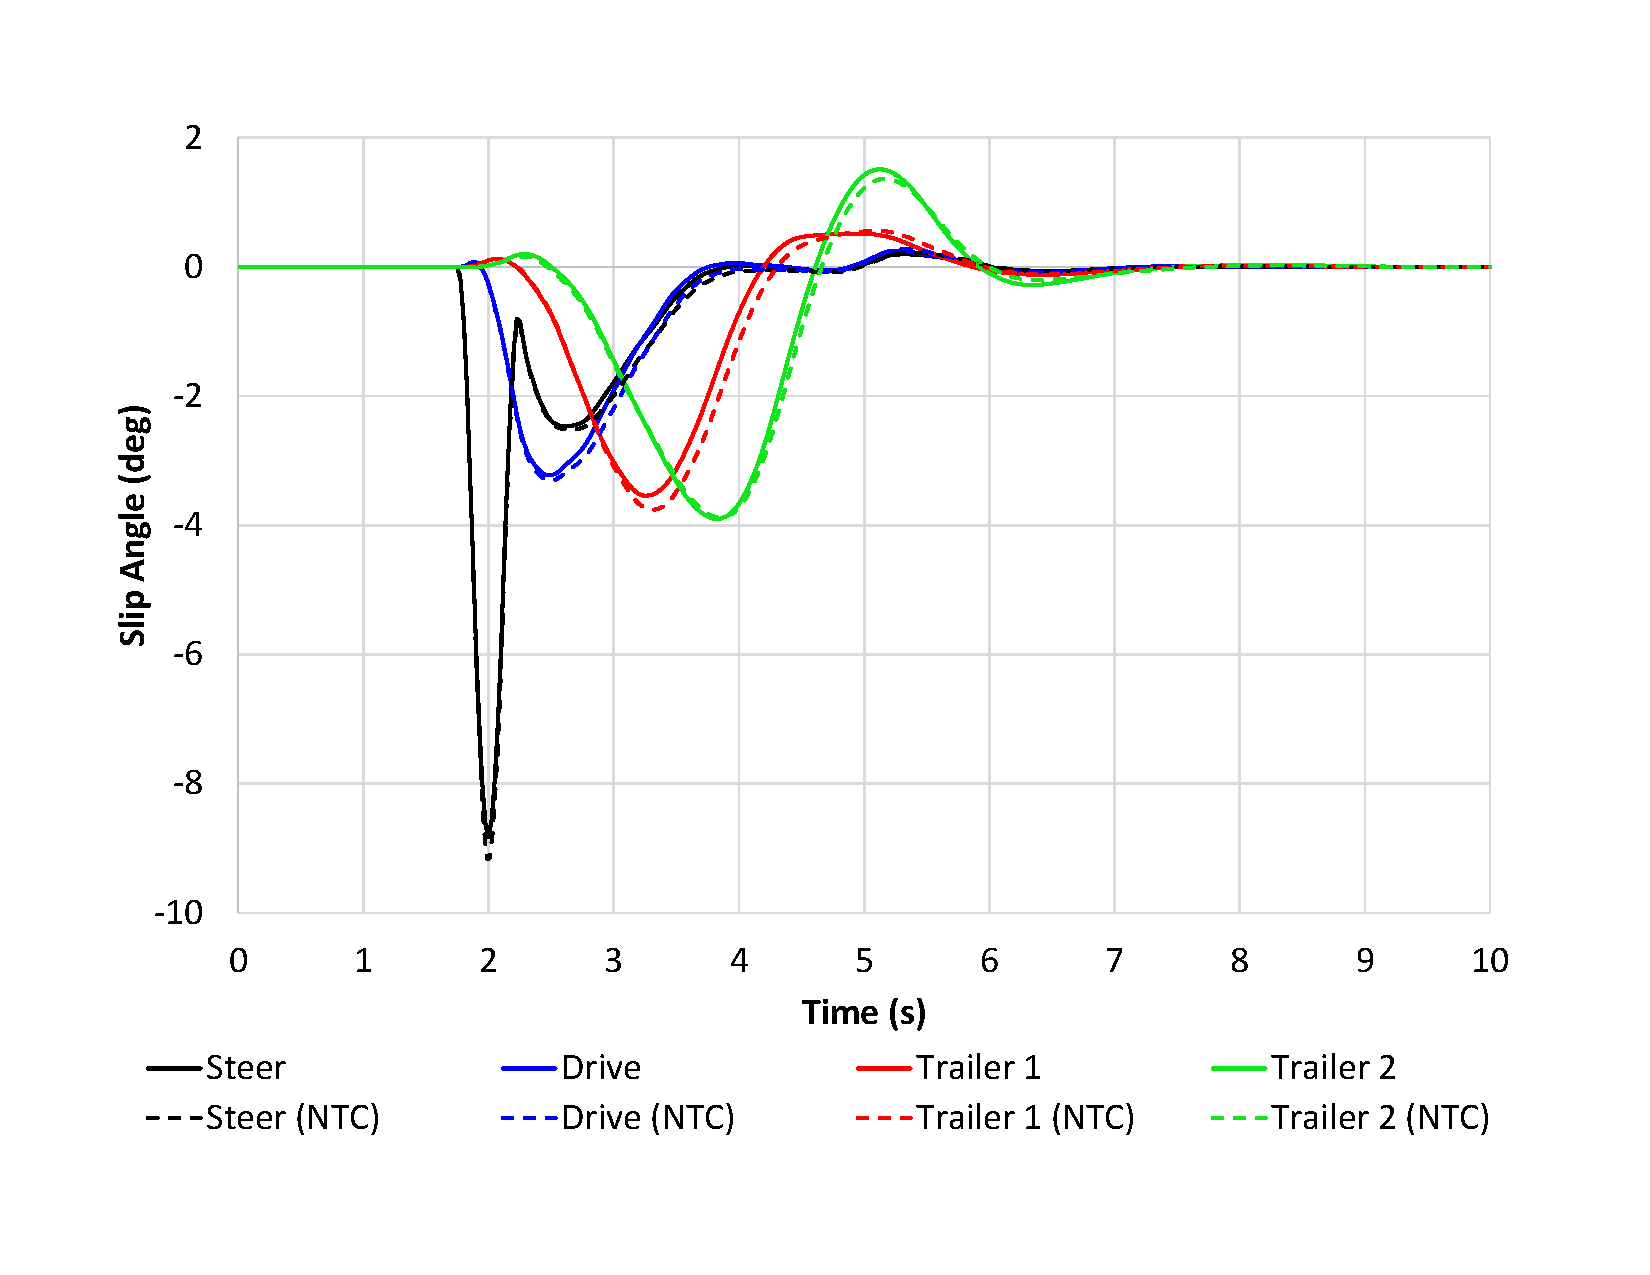
\includegraphics[width=0.8\textwidth]{fig/ntc-b-double_psa}
        \caption{Tyre slip angles from the B-double pulse steer simulations}
        \label{figure:NRC-B-Double_PSa}
    \end{figure}
%----------------------------------------------
%      FIGURE
%----------------------------------------------   

%----------------------------------------------
%      FIGURE
%----------------------------------------------
   \begin{figure}[H]
        \centering
        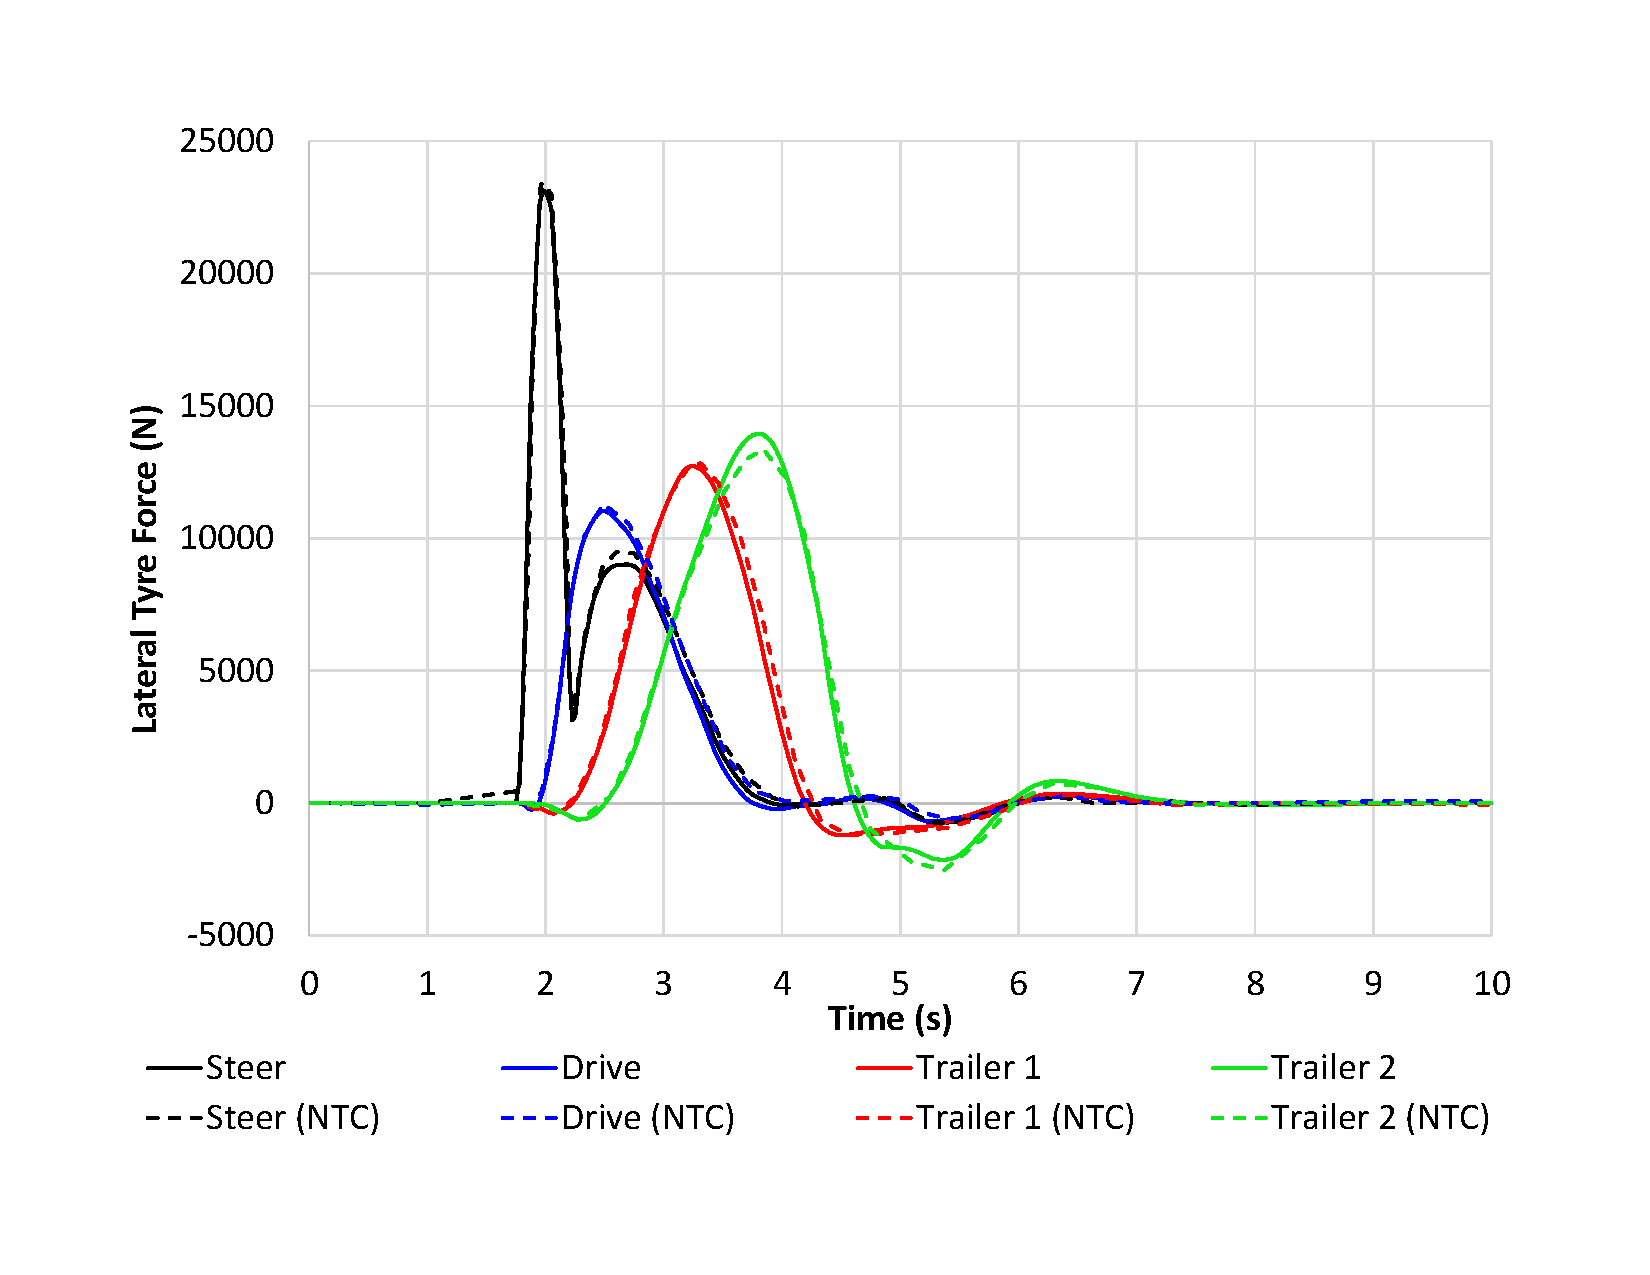
\includegraphics[width=0.8\textwidth]{fig/ntc-b-double_psb}
        \caption{Lateral tyre forces from the B-double pulse steer simulations}
        \label{figure:ntc-b-double_psb}
    \end{figure}
%----------------------------------------------
%      FIGURE
%----------------------------------------------
 
%----------------------------------------------
%      FIGURE
%----------------------------------------------
    \begin{figure}[H]
        \centering
        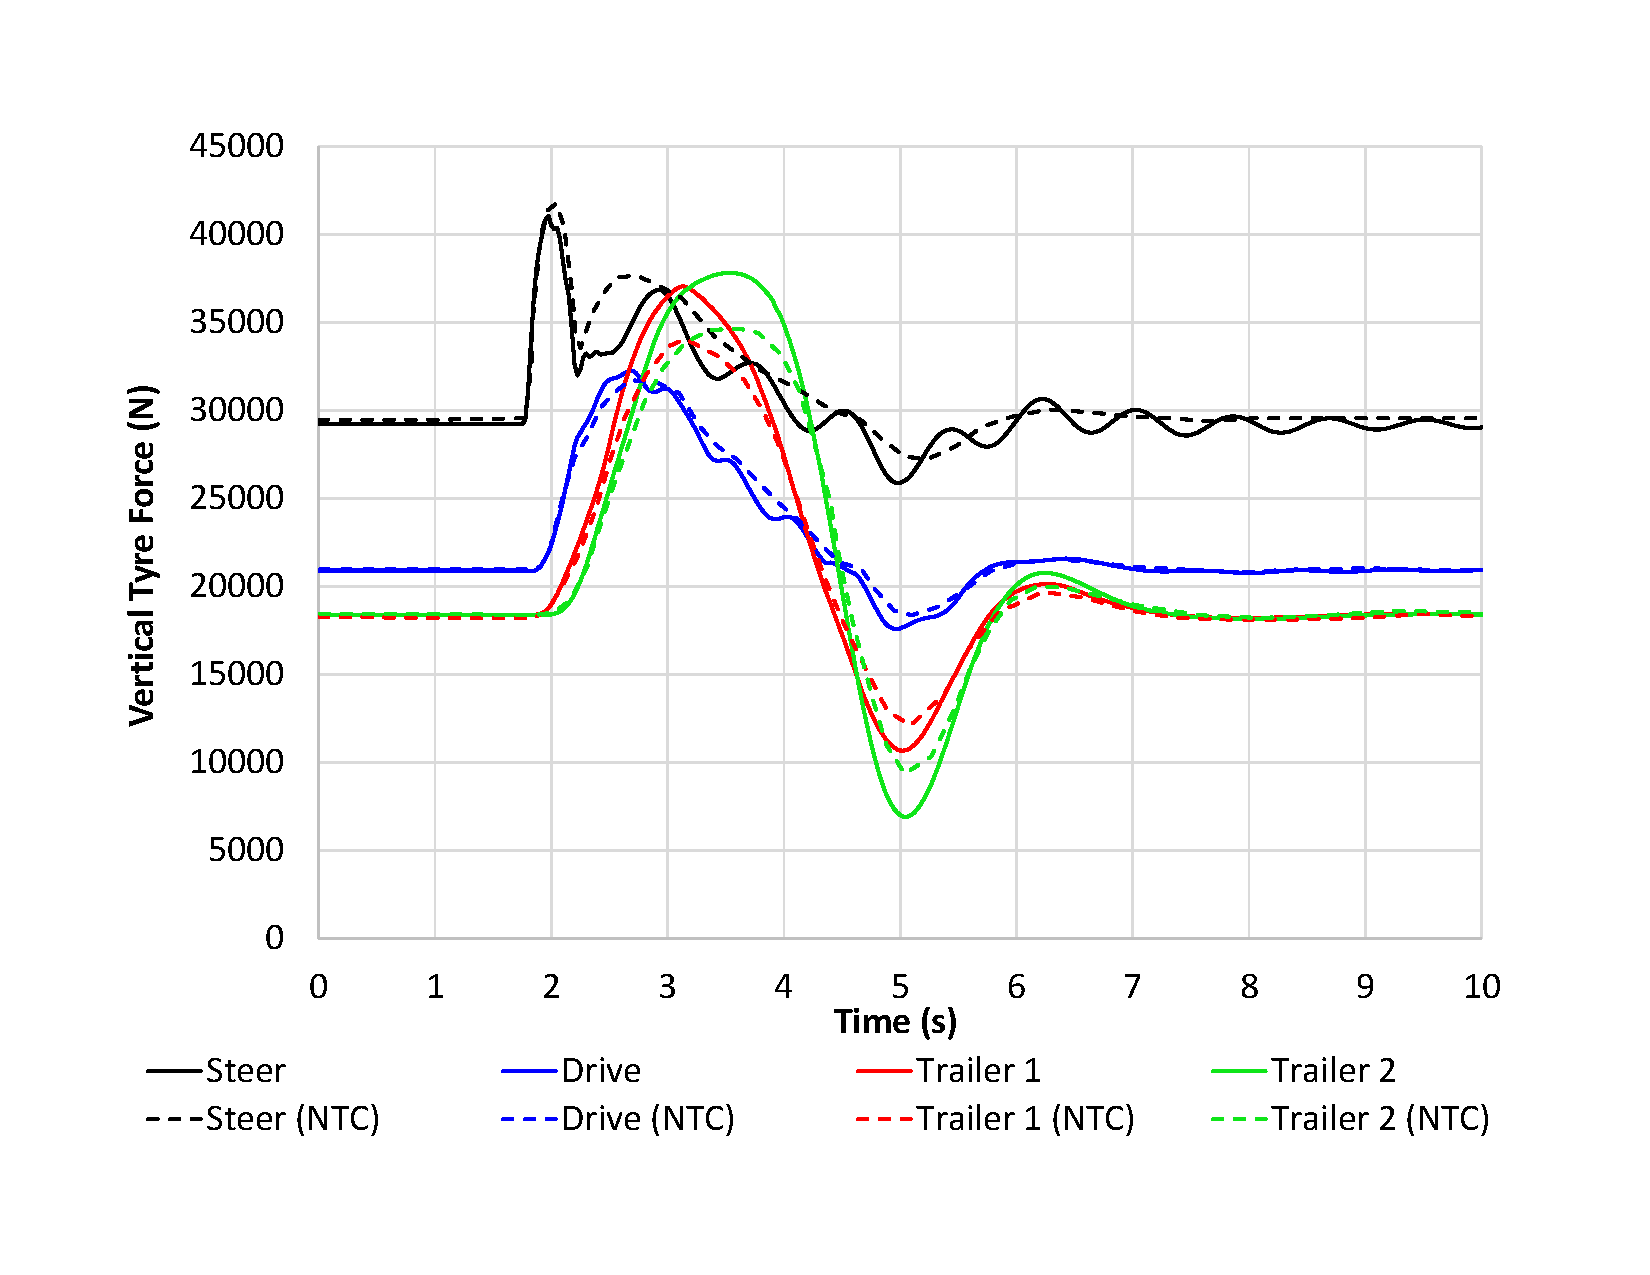
\includegraphics[width=0.8\textwidth]{fig/ntc-b-double_psc}
        \caption{Vertical tyre forces from the B-double pulse steer simulations}
        \label{figure:ntc-b-double_psc}
    \end{figure}
%----------------------------------------------
%      FIGURE
%----------------------------------------------

%----------------------------------------------
%      FIGURE
%----------------------------------------------
    \begin{figure}[H]
        \centering
        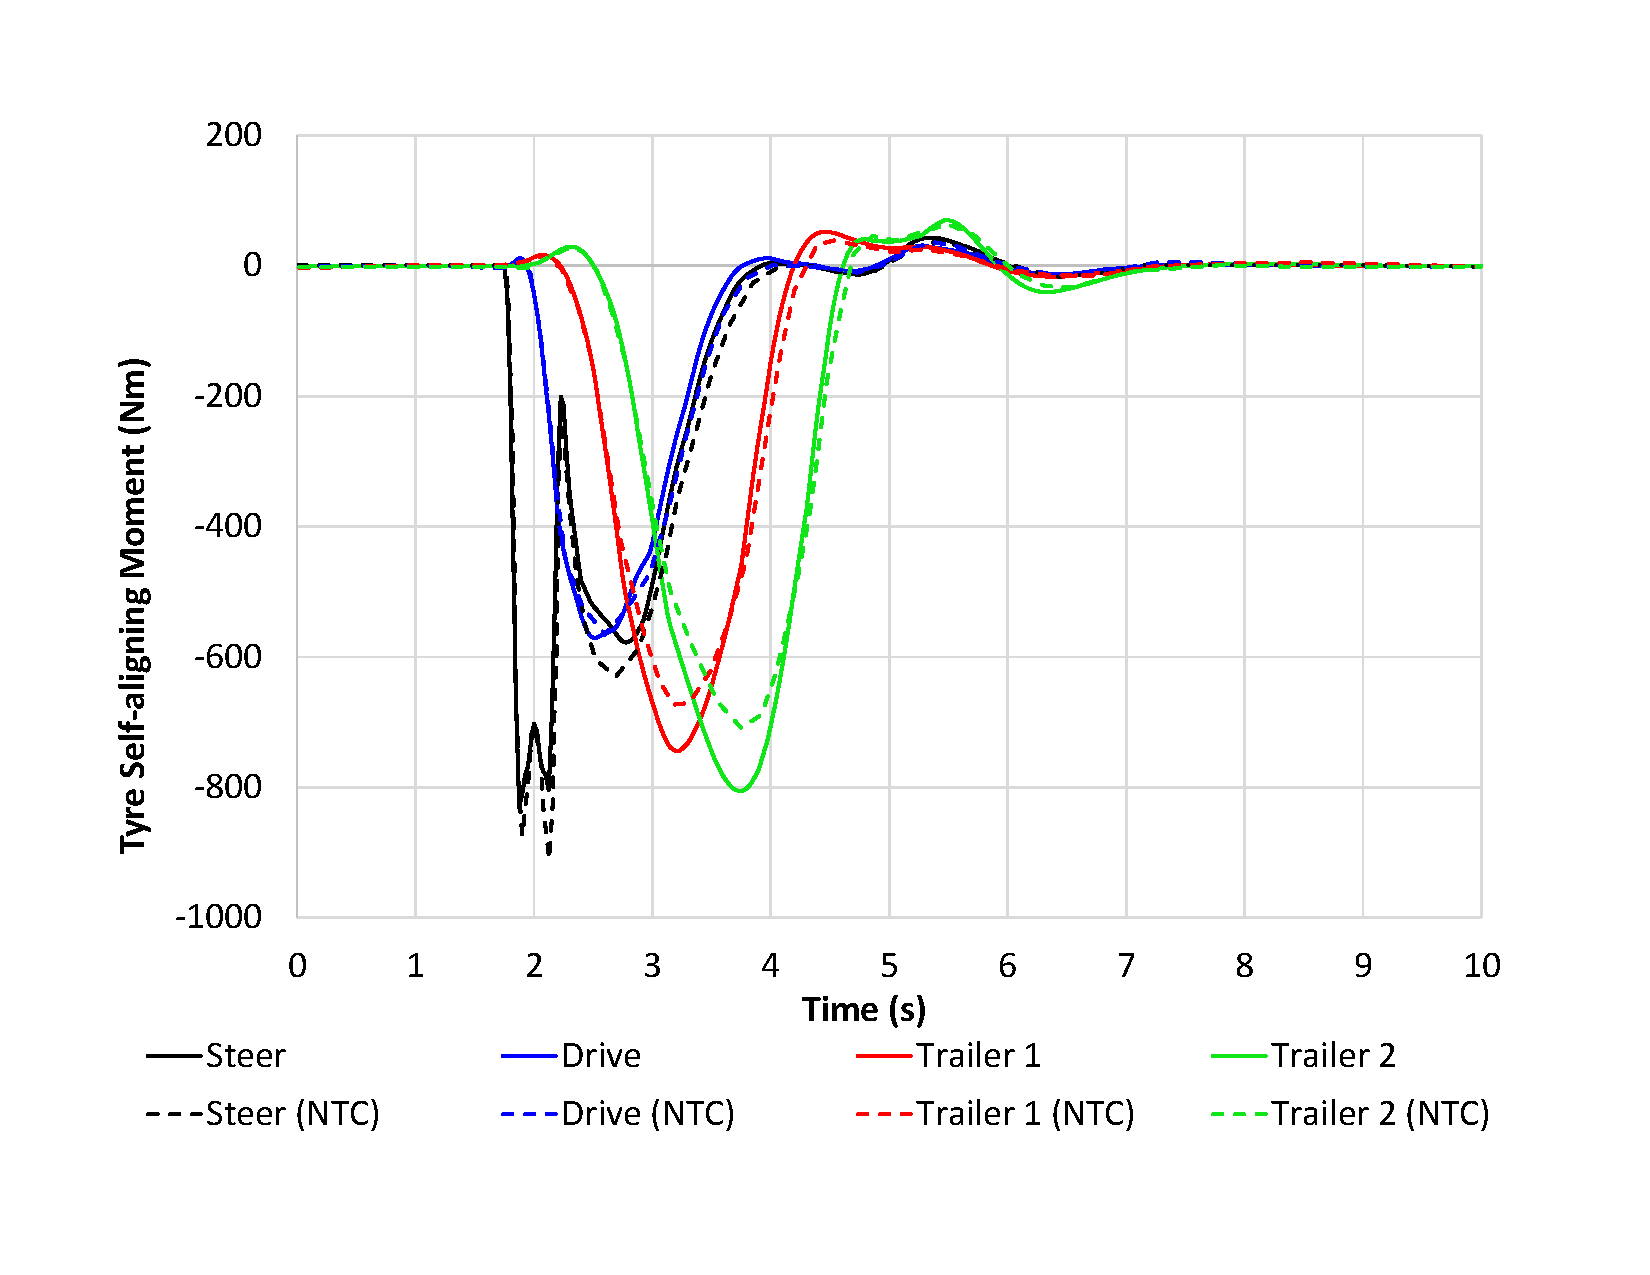
\includegraphics[width=0.8\textwidth]{fig/ntc-b-double_pse}
        \caption{Self-aligning moments from the B-double pulse steer simulations}
        \label{figure:ntc-b-double_pse}
    \end{figure}
%----------------------------------------------
%      FIGURE
%----------------------------------------------

%----------------------------------------------
%      FIGURE
%----------------------------------------------
    \begin{figure}[H]
        \centering
        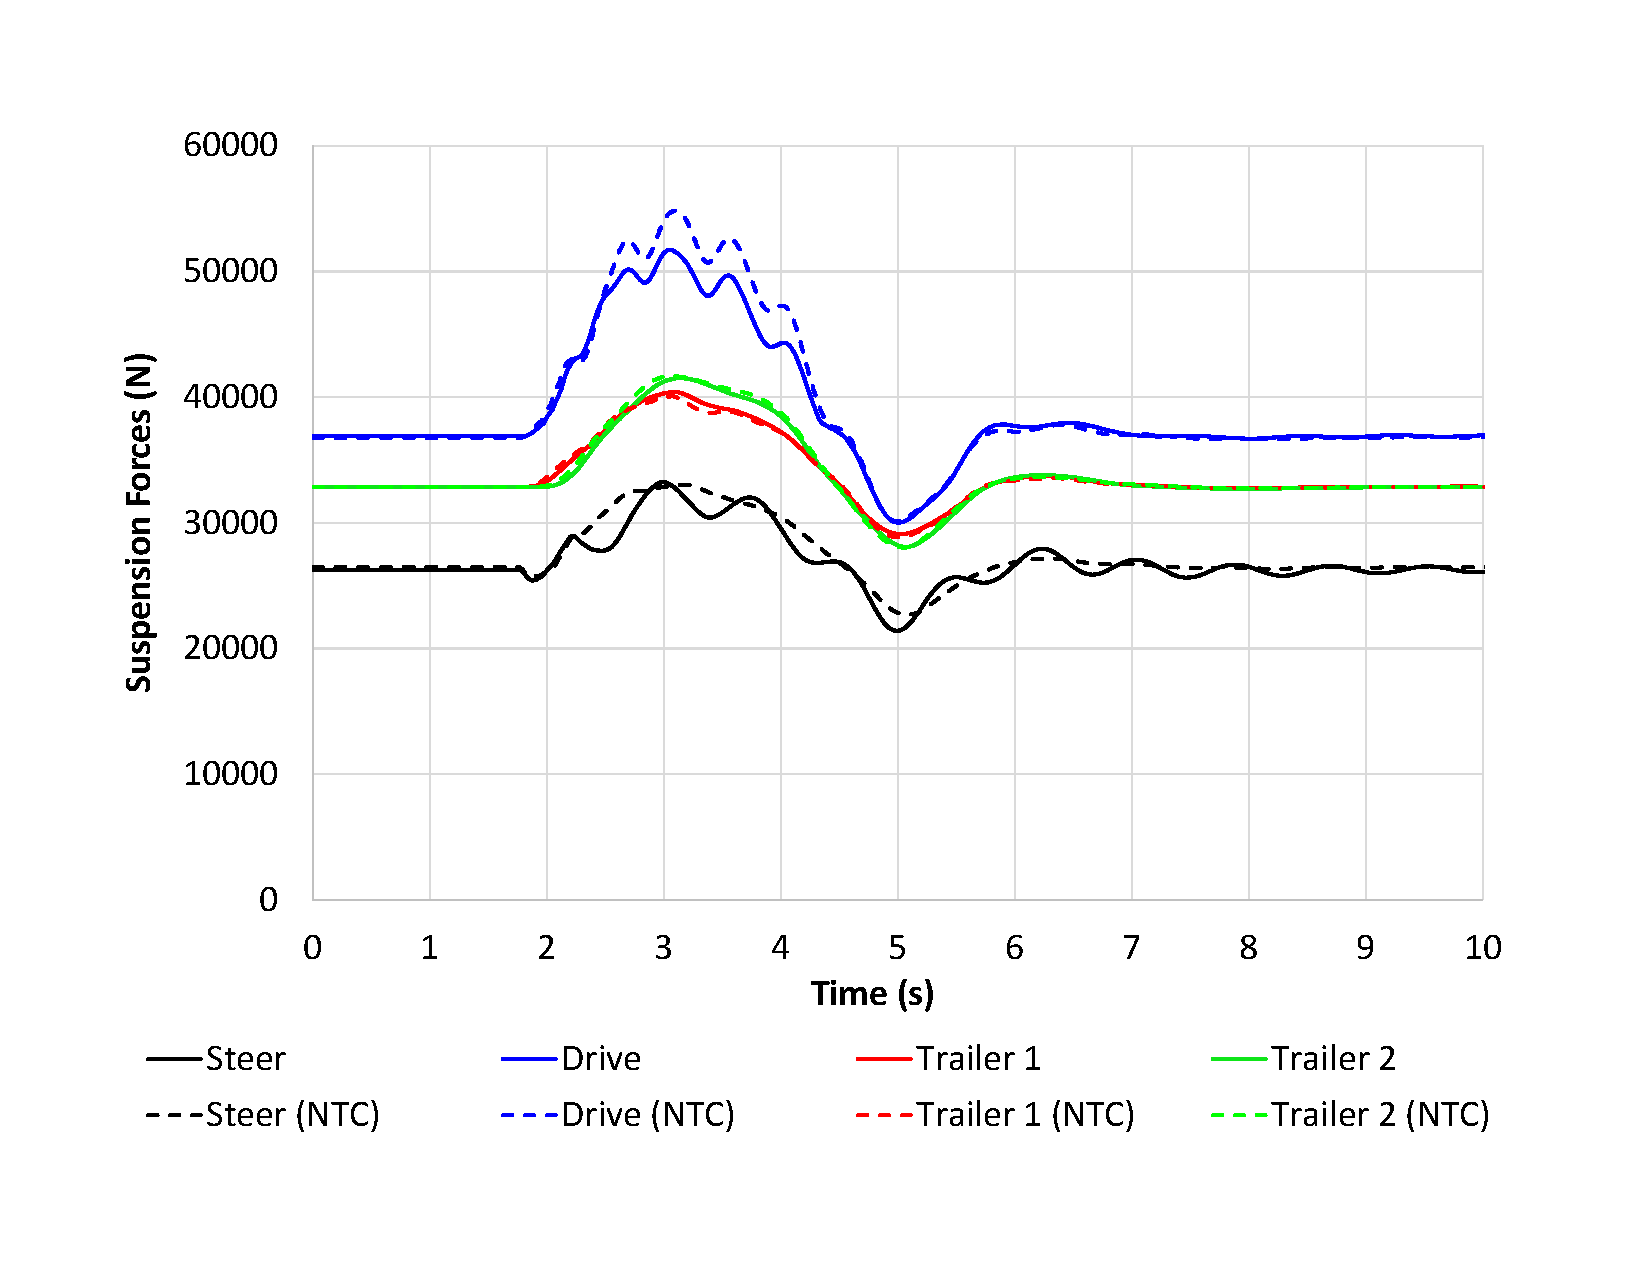
\includegraphics[width=0.8\textwidth]{fig/ntc-b-double_psf}
        \caption{Suspension forces from the B-double pulse steer simulations}
        \label{figure:ntc-b-double_psf}
    \end{figure}
%----------------------------------------------
%      FIGURE
%----------------------------------------------

%----------------------------------------------
%      FIGURE
%----------------------------------------------
    \begin{figure}[H]
        \centering
        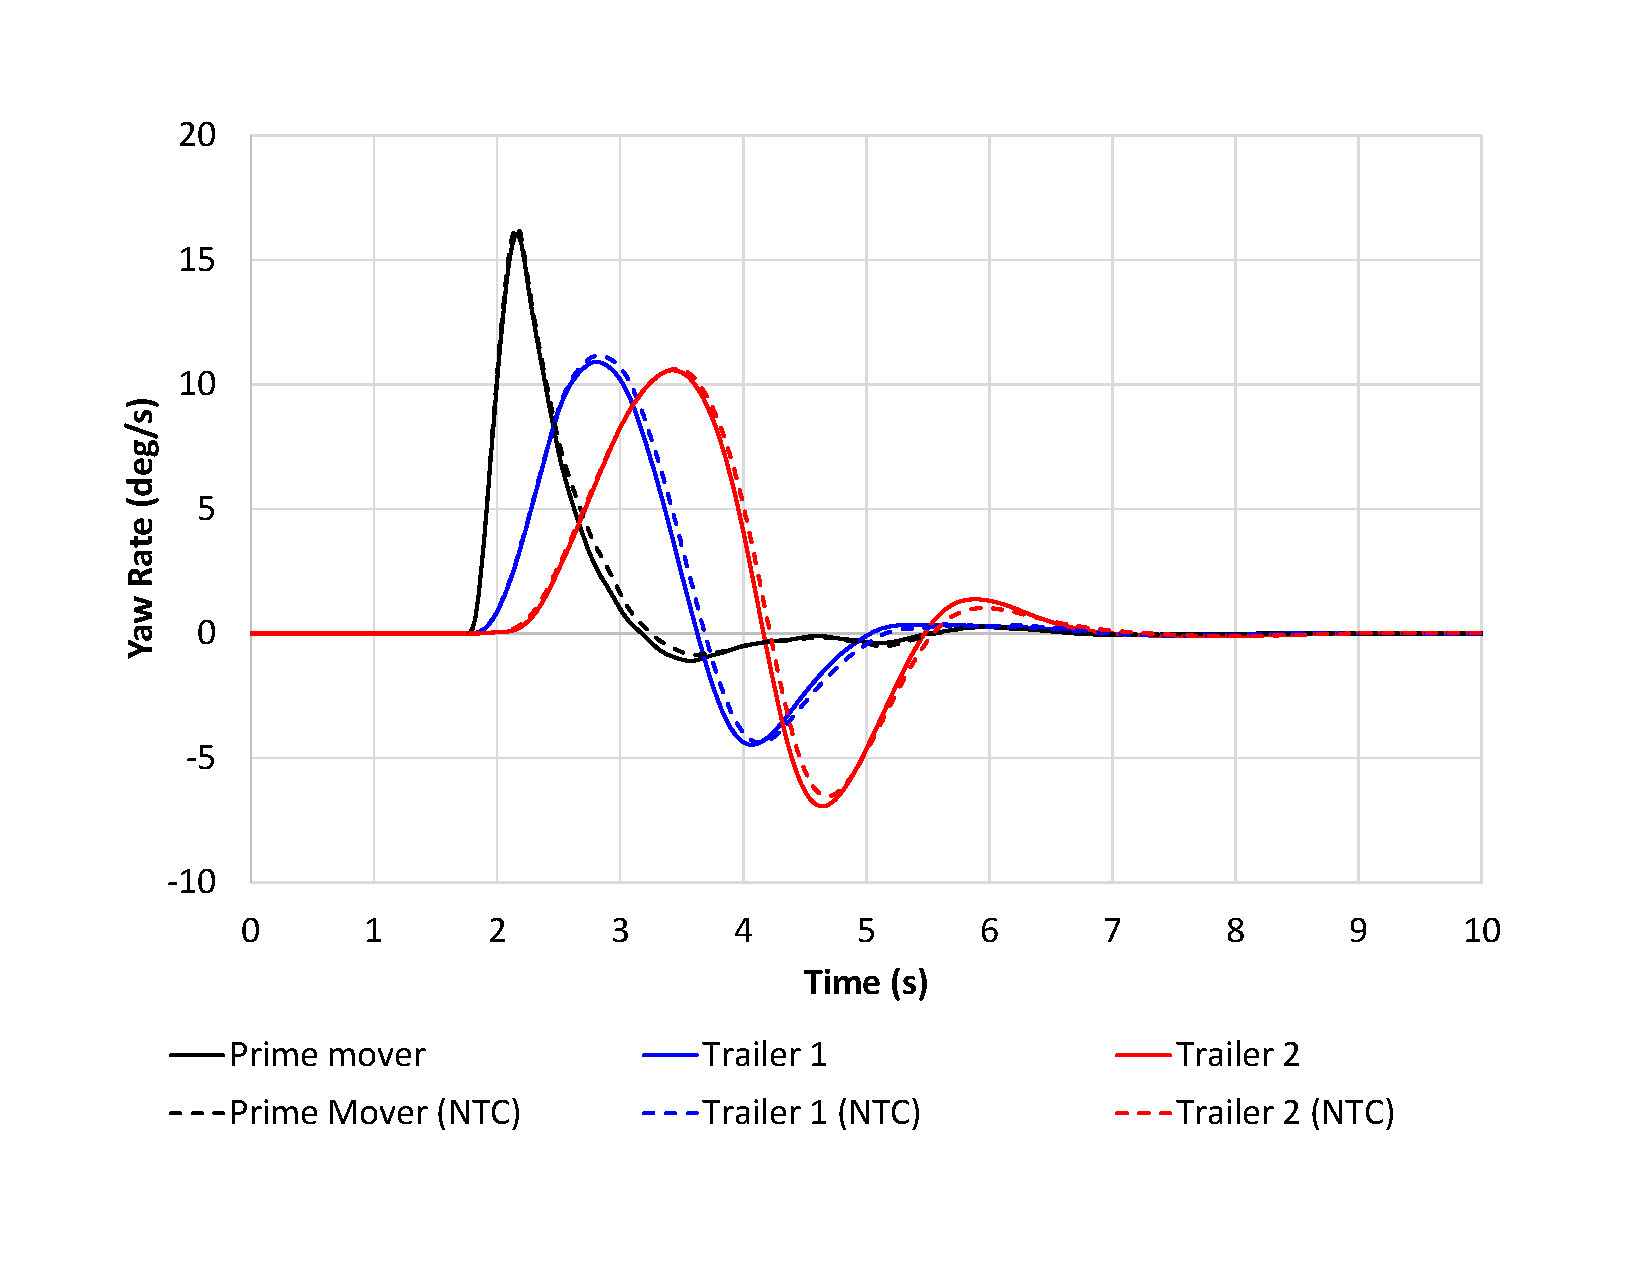
\includegraphics[width=0.8\textwidth]{fig/ntc-b-double_psg}
        \caption{Yaw rates from the B-double pulse steer simulations}
        \label{figure:ntc-b-double_psg}
    \end{figure}
%----------------------------------------------
%      FIGURE
%----------------------------------------------

%----------------------------------------------
%      FIGURE
%----------------------------------------------
    \begin{figure}[H]
        \centering
        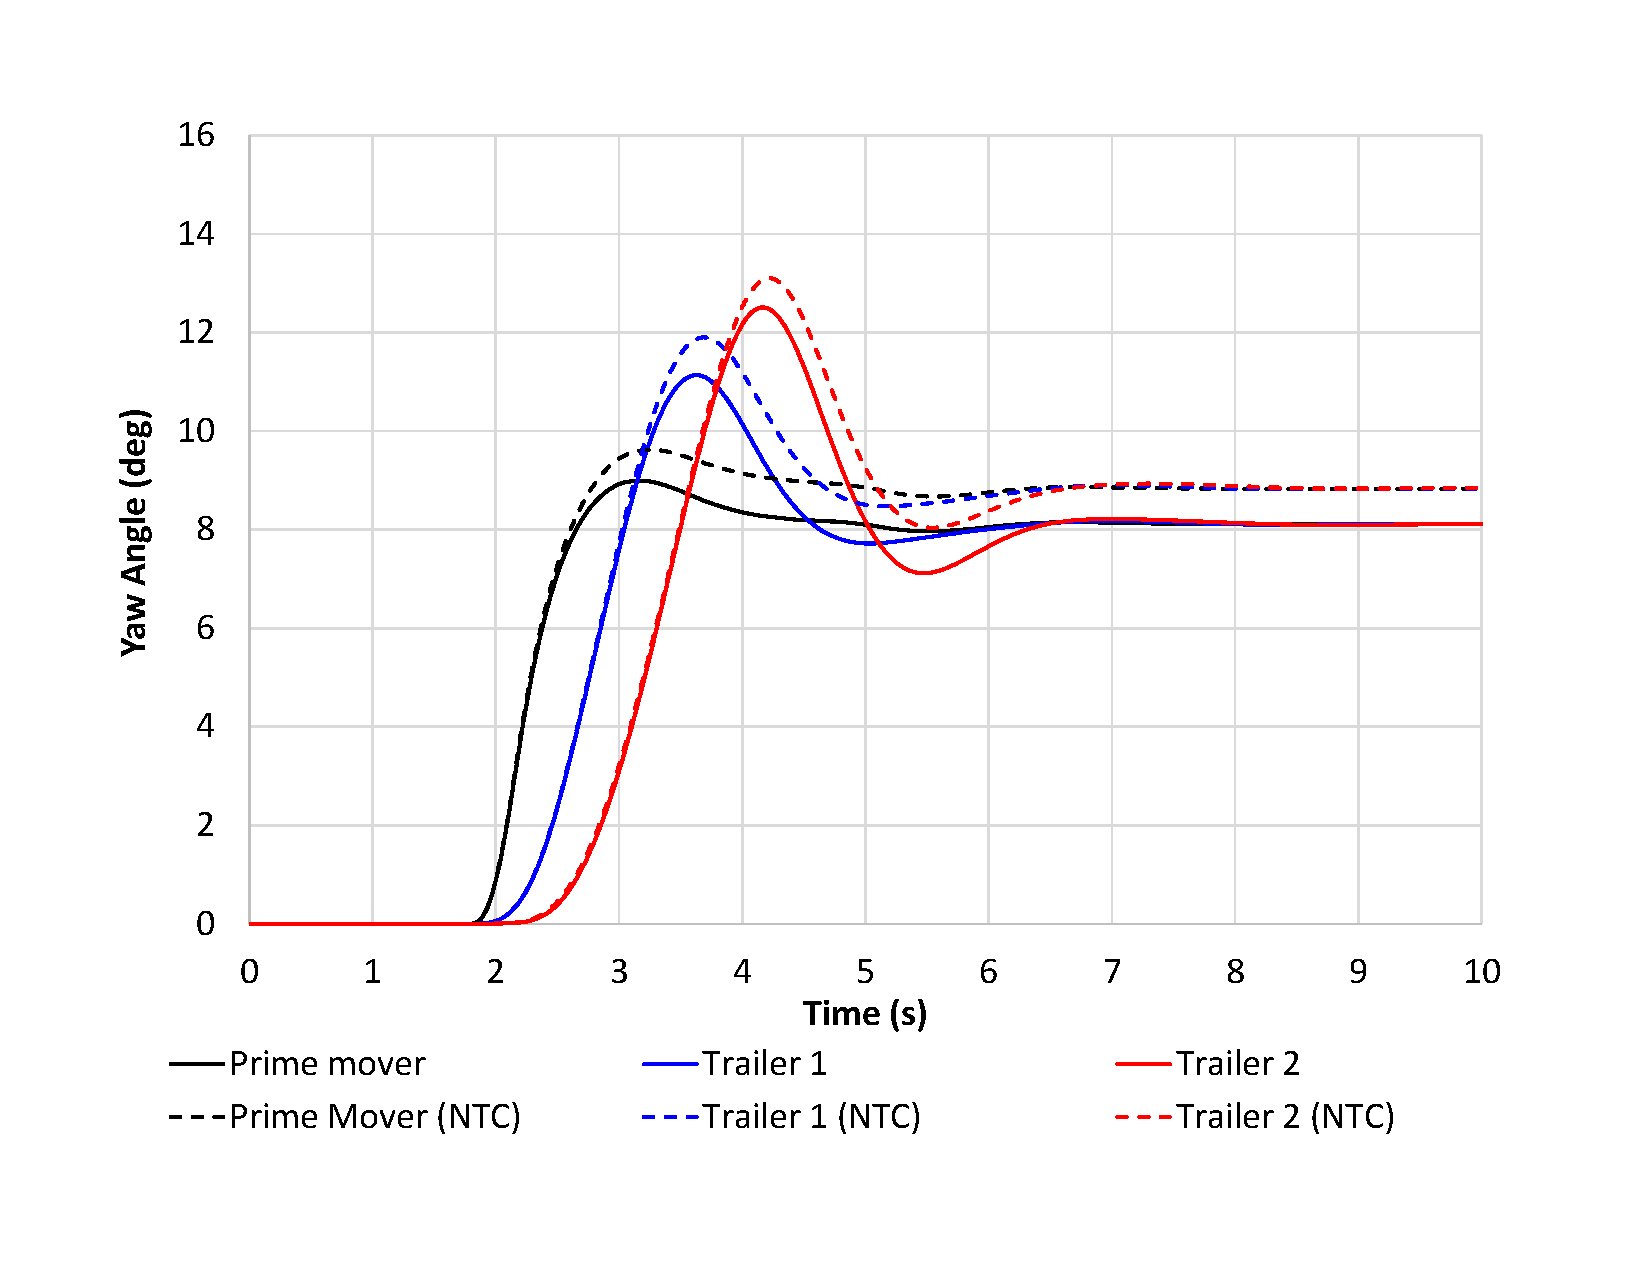
\includegraphics[width=0.8\textwidth]{fig/ntc-b-double_psh}
        \caption{Yaw angles from the B-double pulse steer simulations}
        \label{figure:ntc-b-double_psh}
    \end{figure}
%----------------------------------------------
%      FIGURE
%----------------------------------------------

%----------------------------------------------
%      FIGURE
%----------------------------------------------
    \begin{figure}[H]
        \centering
        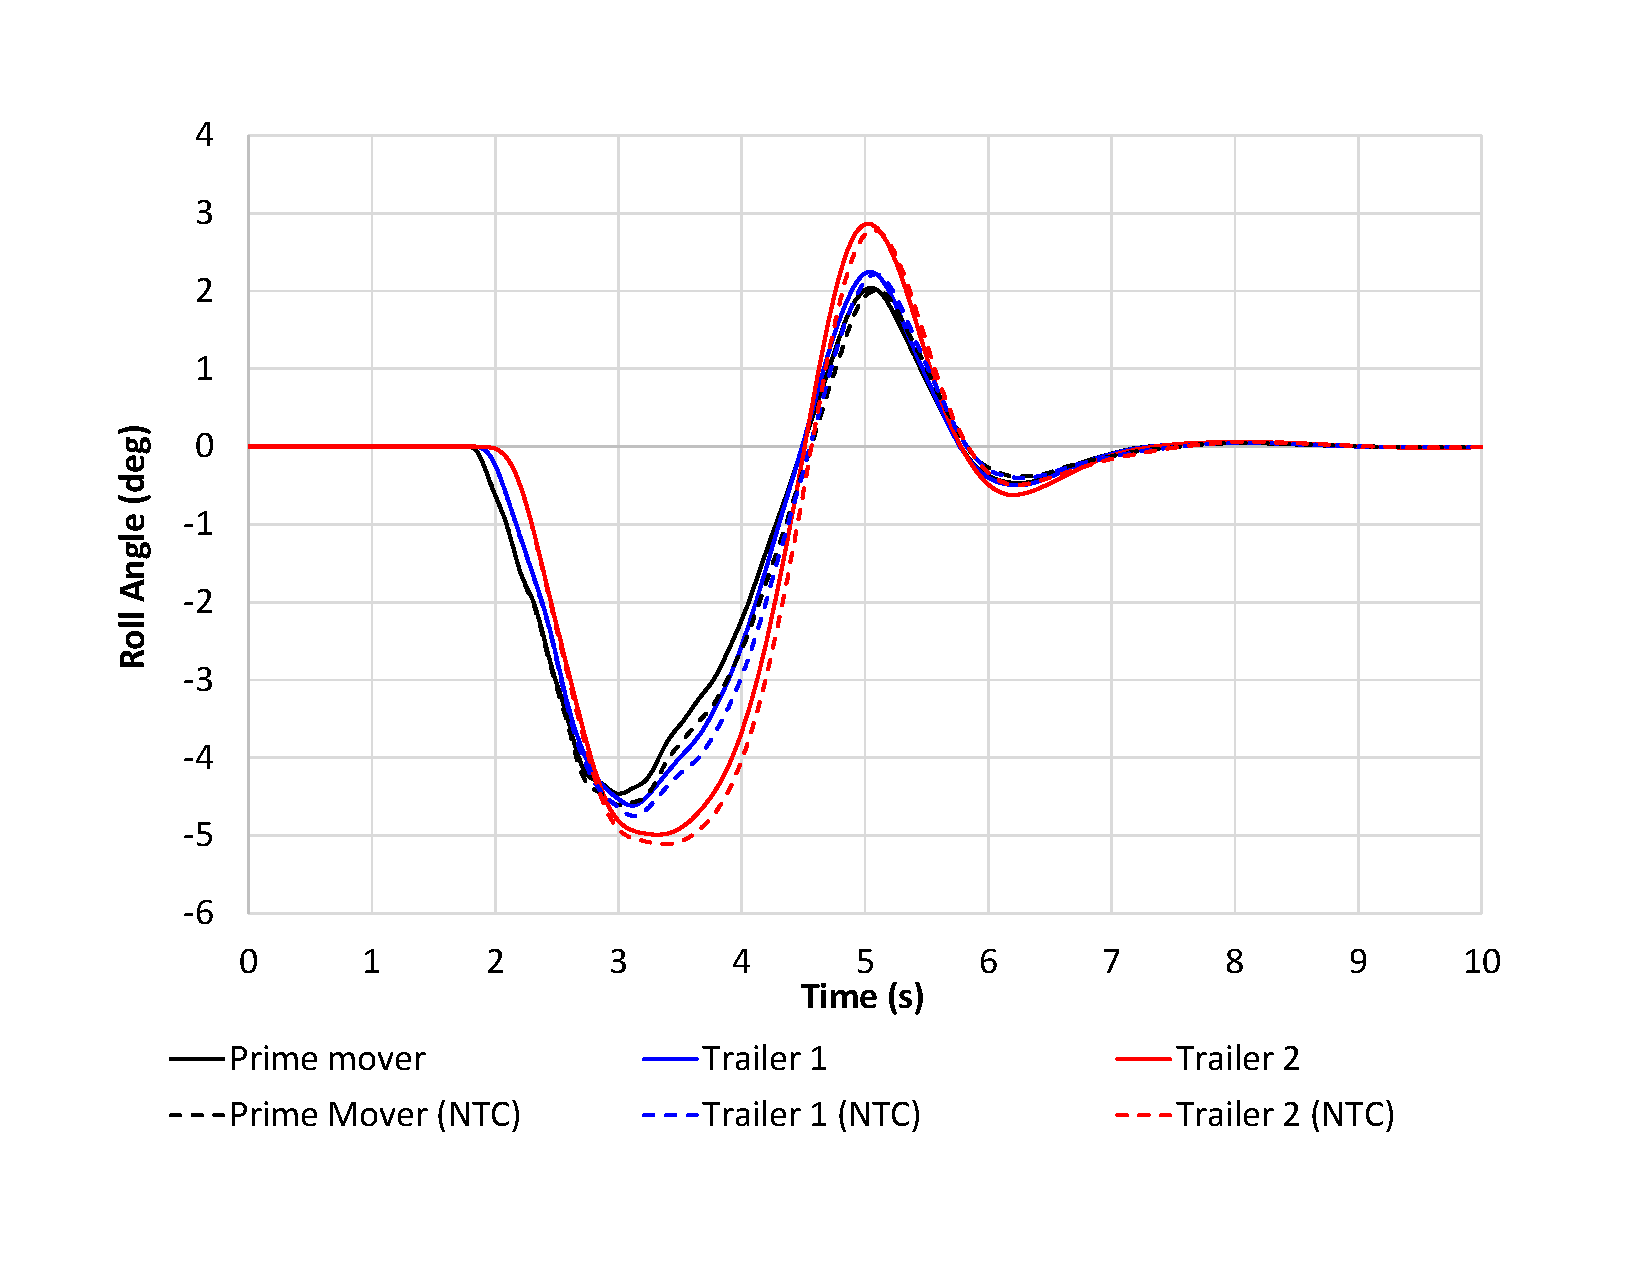
\includegraphics[width=0.8\textwidth]{fig/ntc-b-double_psi}
        \caption{Roll angles from the B-double pulse steer simulations}
        \label{figure:ntc-b-double_psi}
    \end{figure}
%----------------------------------------------
%      FIGURE
%----------------------------------------------

%----------------------------------------------
%      FIGURE
%----------------------------------------------
    \begin{figure}[H]
        \centering
        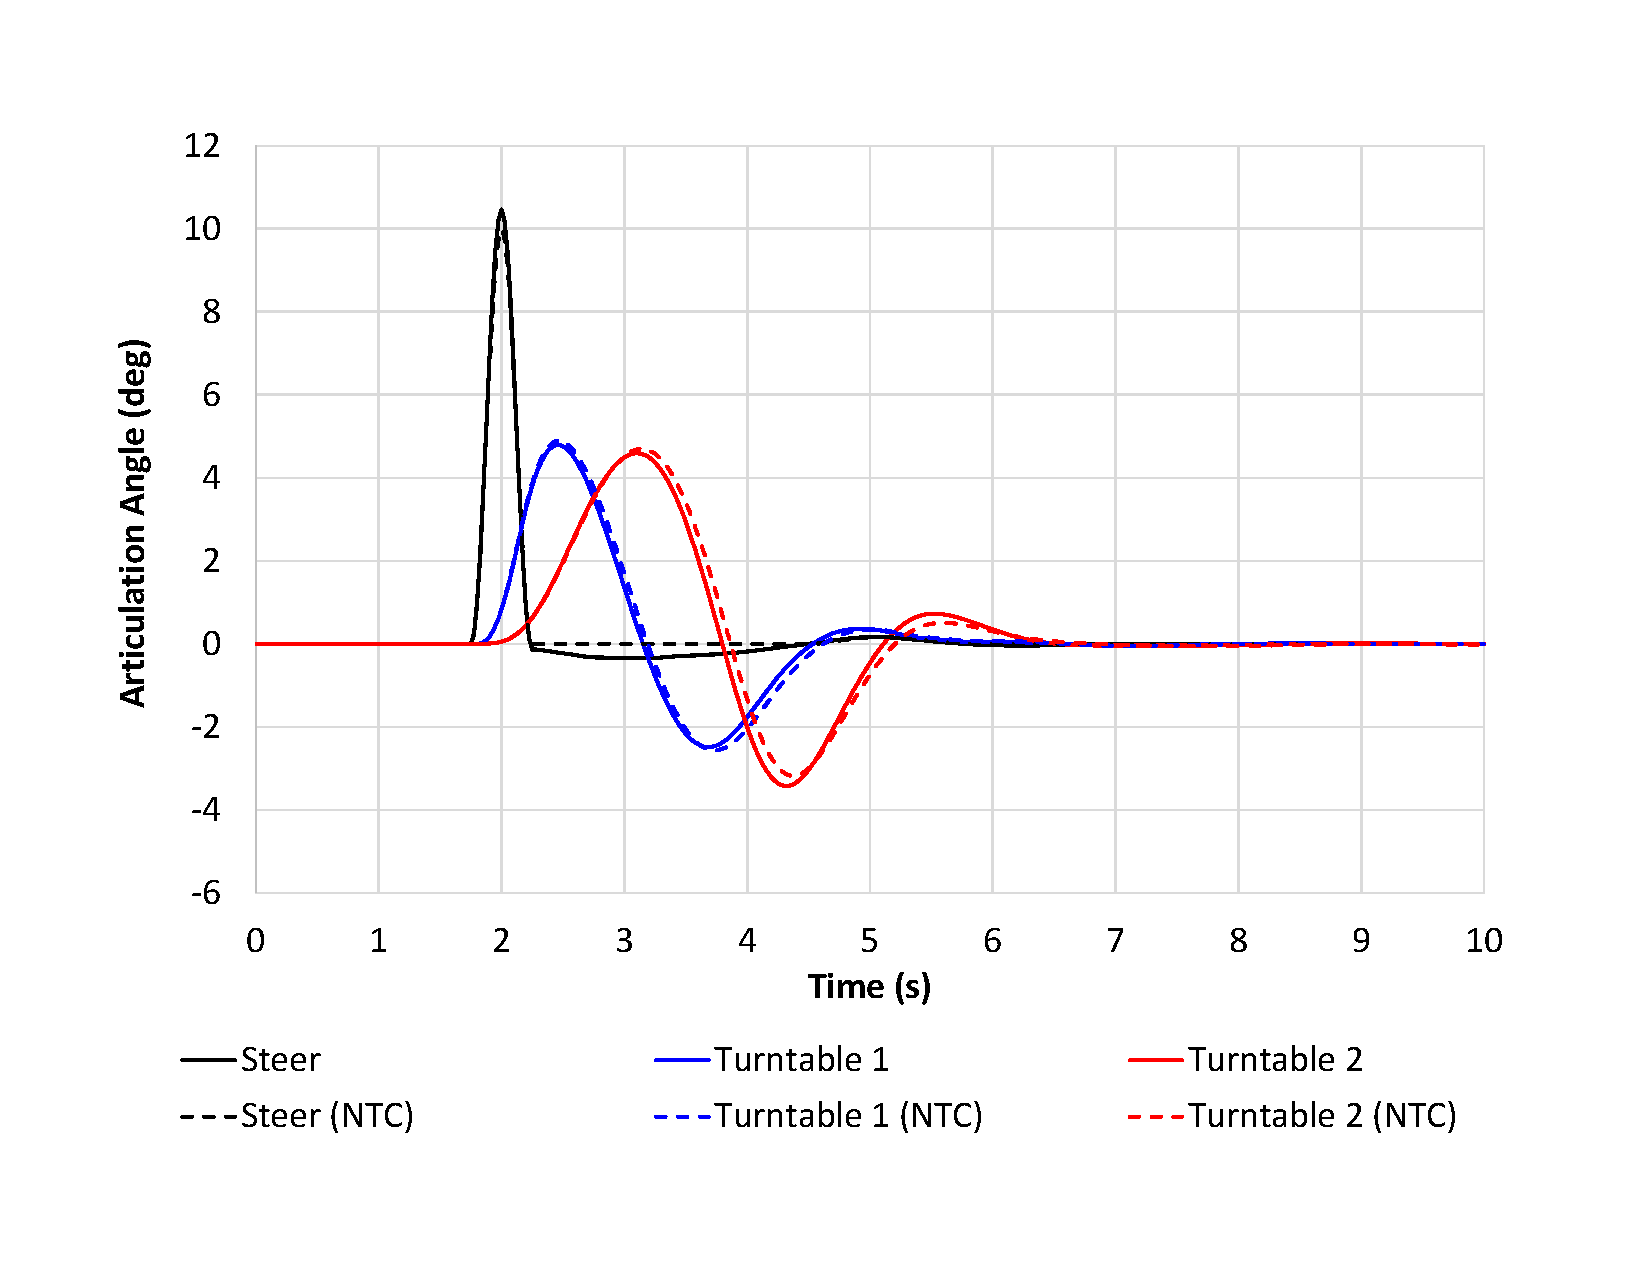
\includegraphics[width=0.8\textwidth]{fig/ntc-b-double_psj}
        \caption{Articulation angles from the B-double pulse steer simulations}
        \label{figure:ntc-b-double_psj}
    \end{figure}
%----------------------------------------------
%      FIGURE
%----------------------------------------------

%----------------------------------------------
%      FIGURE
%----------------------------------------------
    \begin{figure}[H]
        \centering
        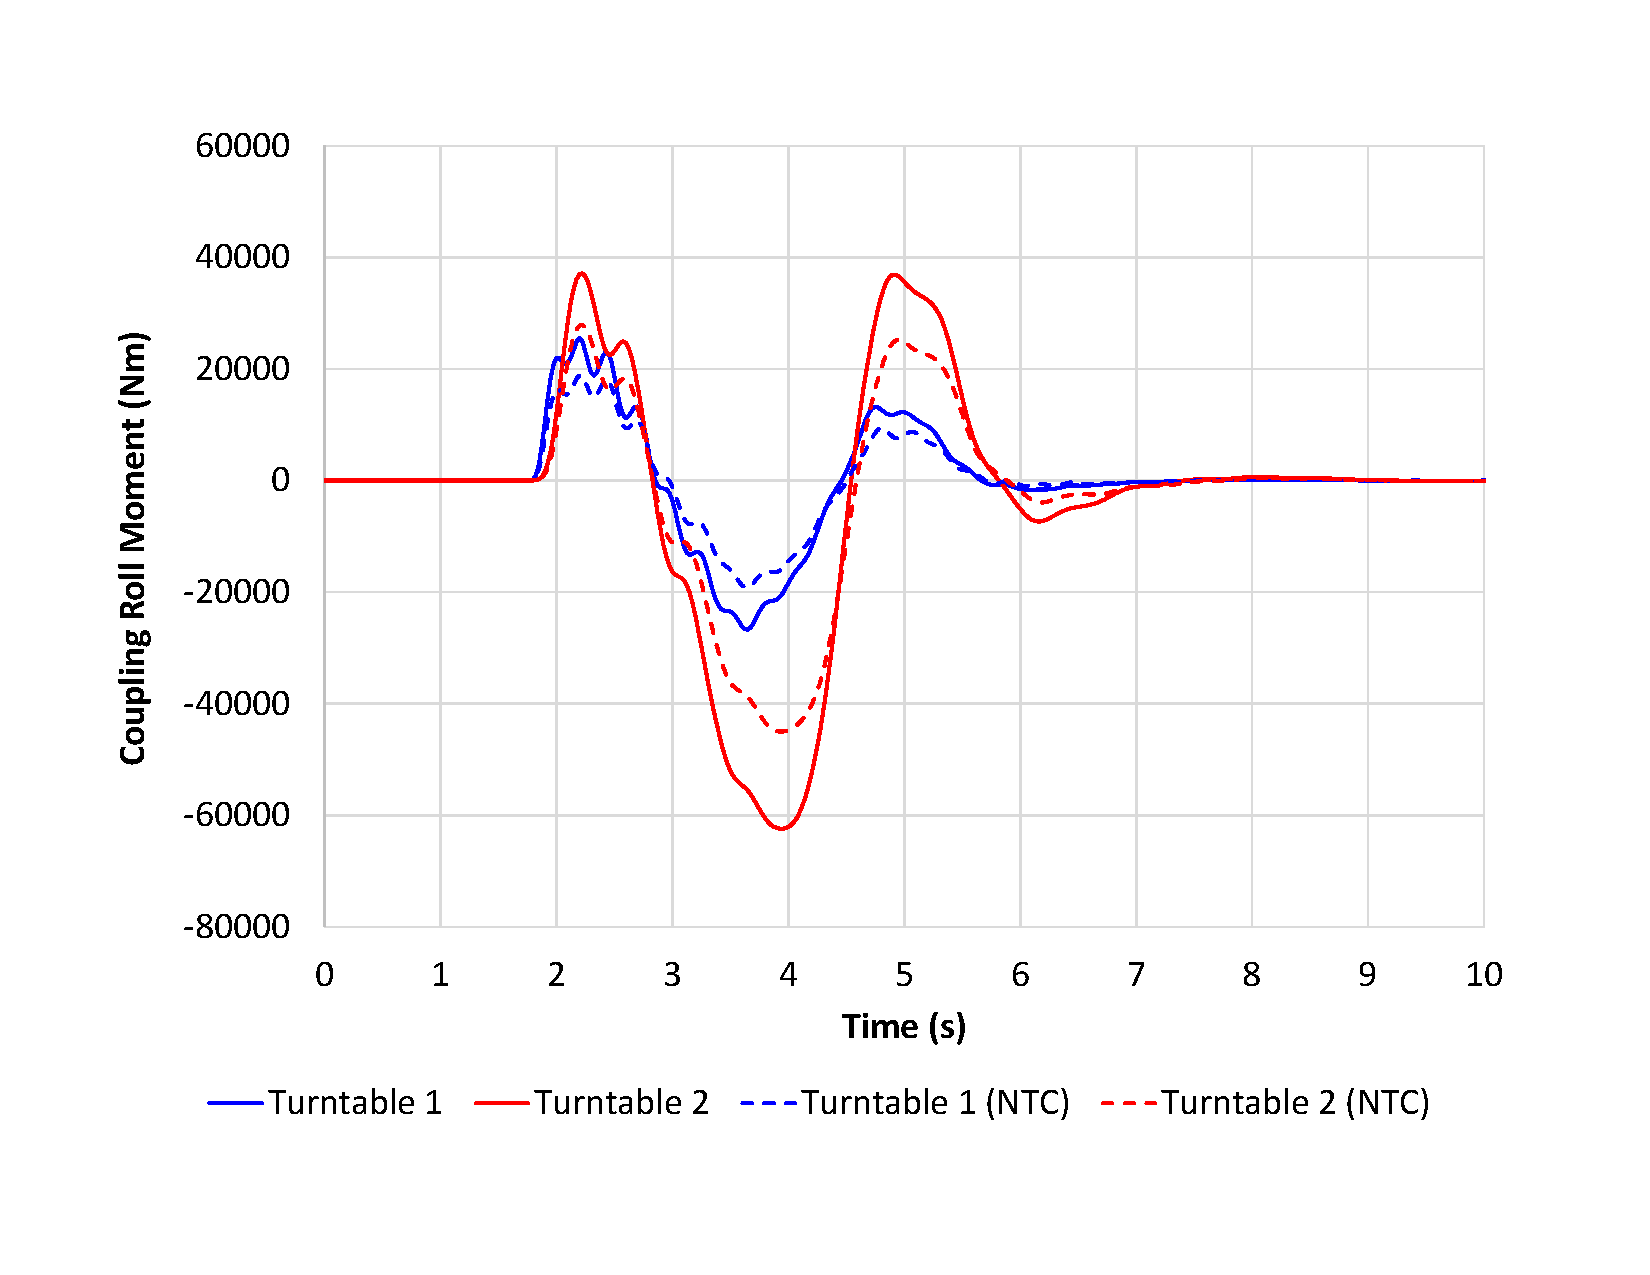
\includegraphics[width=0.8\textwidth]{fig/ntc-b-double_psk}
        \caption{Coupling roll moments from the B-double pulse steer simulations}
        \label{figure:ntc-b-double_psk}
    \end{figure}
%----------------------------------------------
%      FIGURE
%----------------------------------------------

%----------------------------------------------
%      FIGURE
%----------------------------------------------
    \begin{figure}[H]
        \centering
        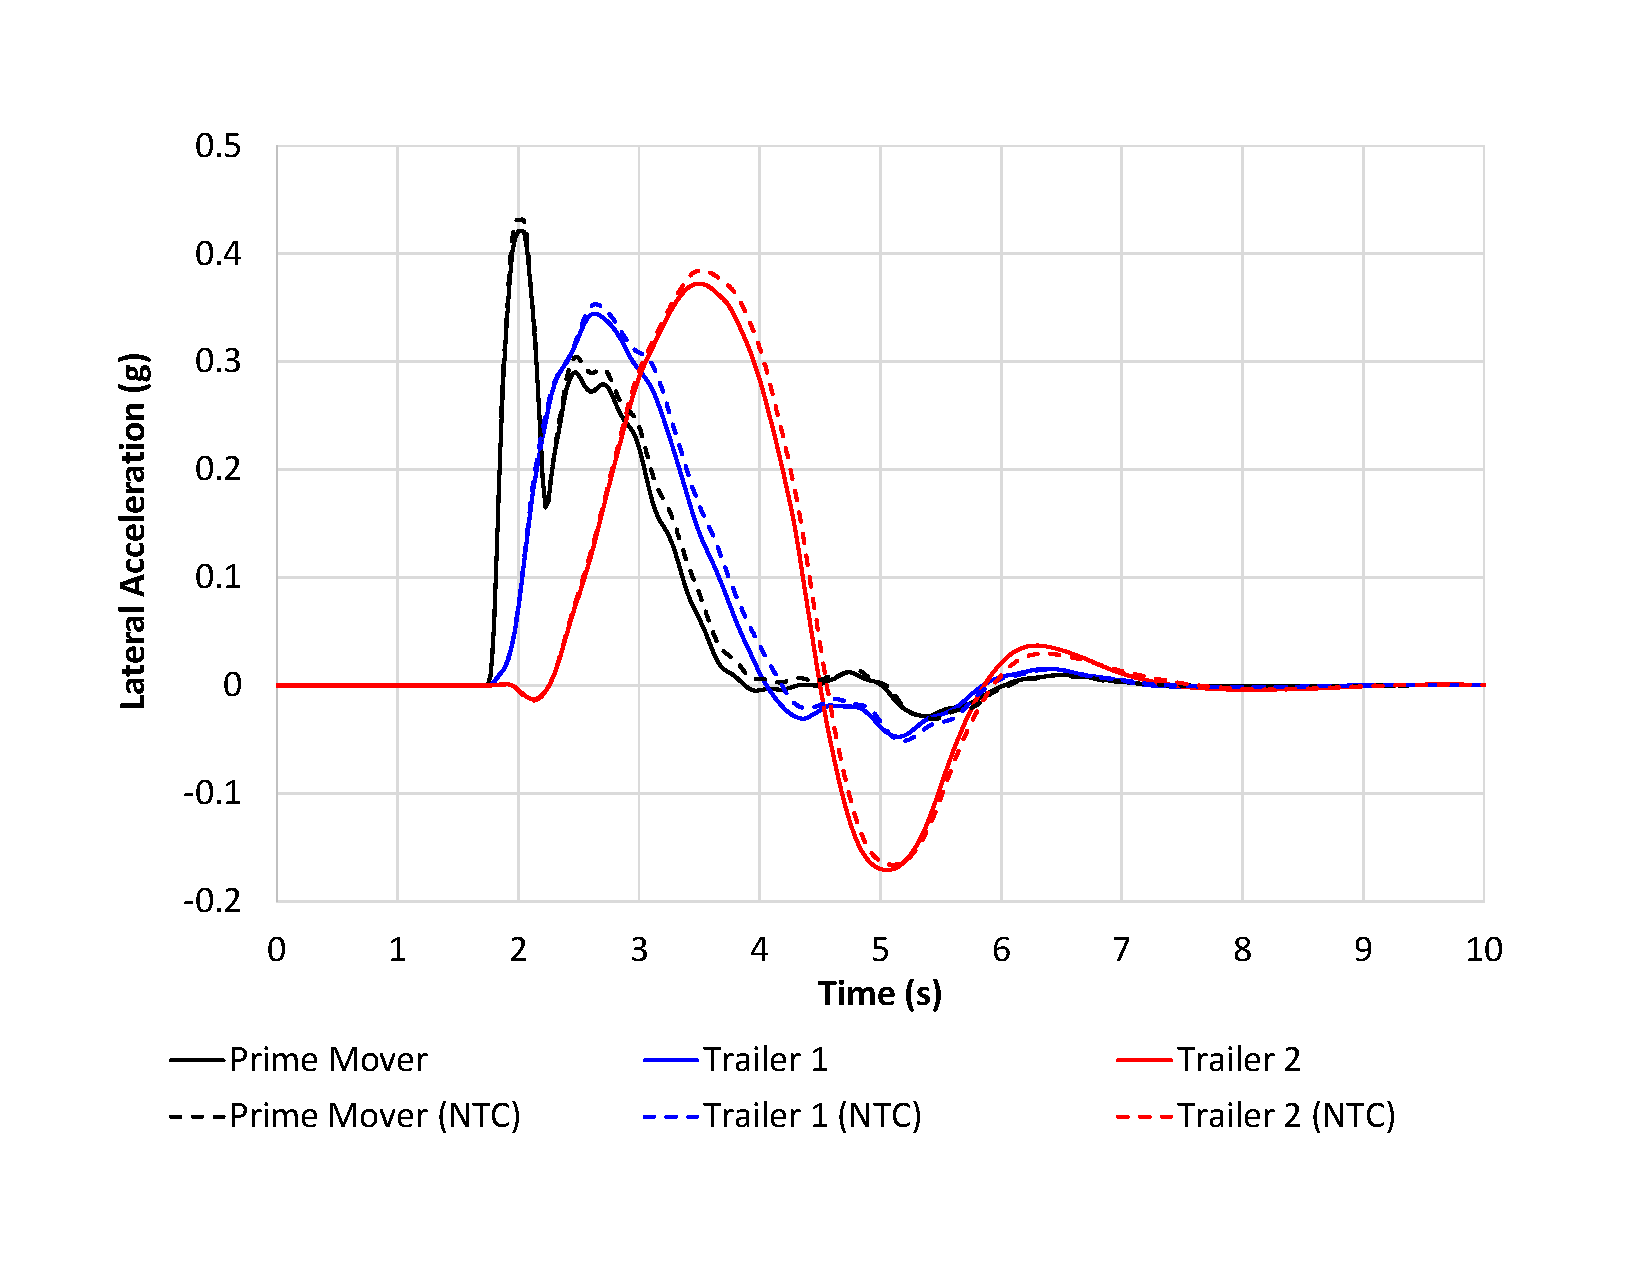
\includegraphics[width=0.8\textwidth]{fig/ntc-b-double_psl}
        \caption{Lateral accelerations from the B-double pulse steer simulations}
        \label{figure:ntc-b-double_psl}
    \end{figure}
%----------------------------------------------
%      FIGURE
%----------------------------------------------

%      SUBSECTION
%----------------------------------------------
\subsection{B-double Step Steer}\label{appendix:b-double-validation-ss}

%----------------------------------------------
%      FIGURE
%----------------------------------------------
    \begin{figure}[H]
        \centering
        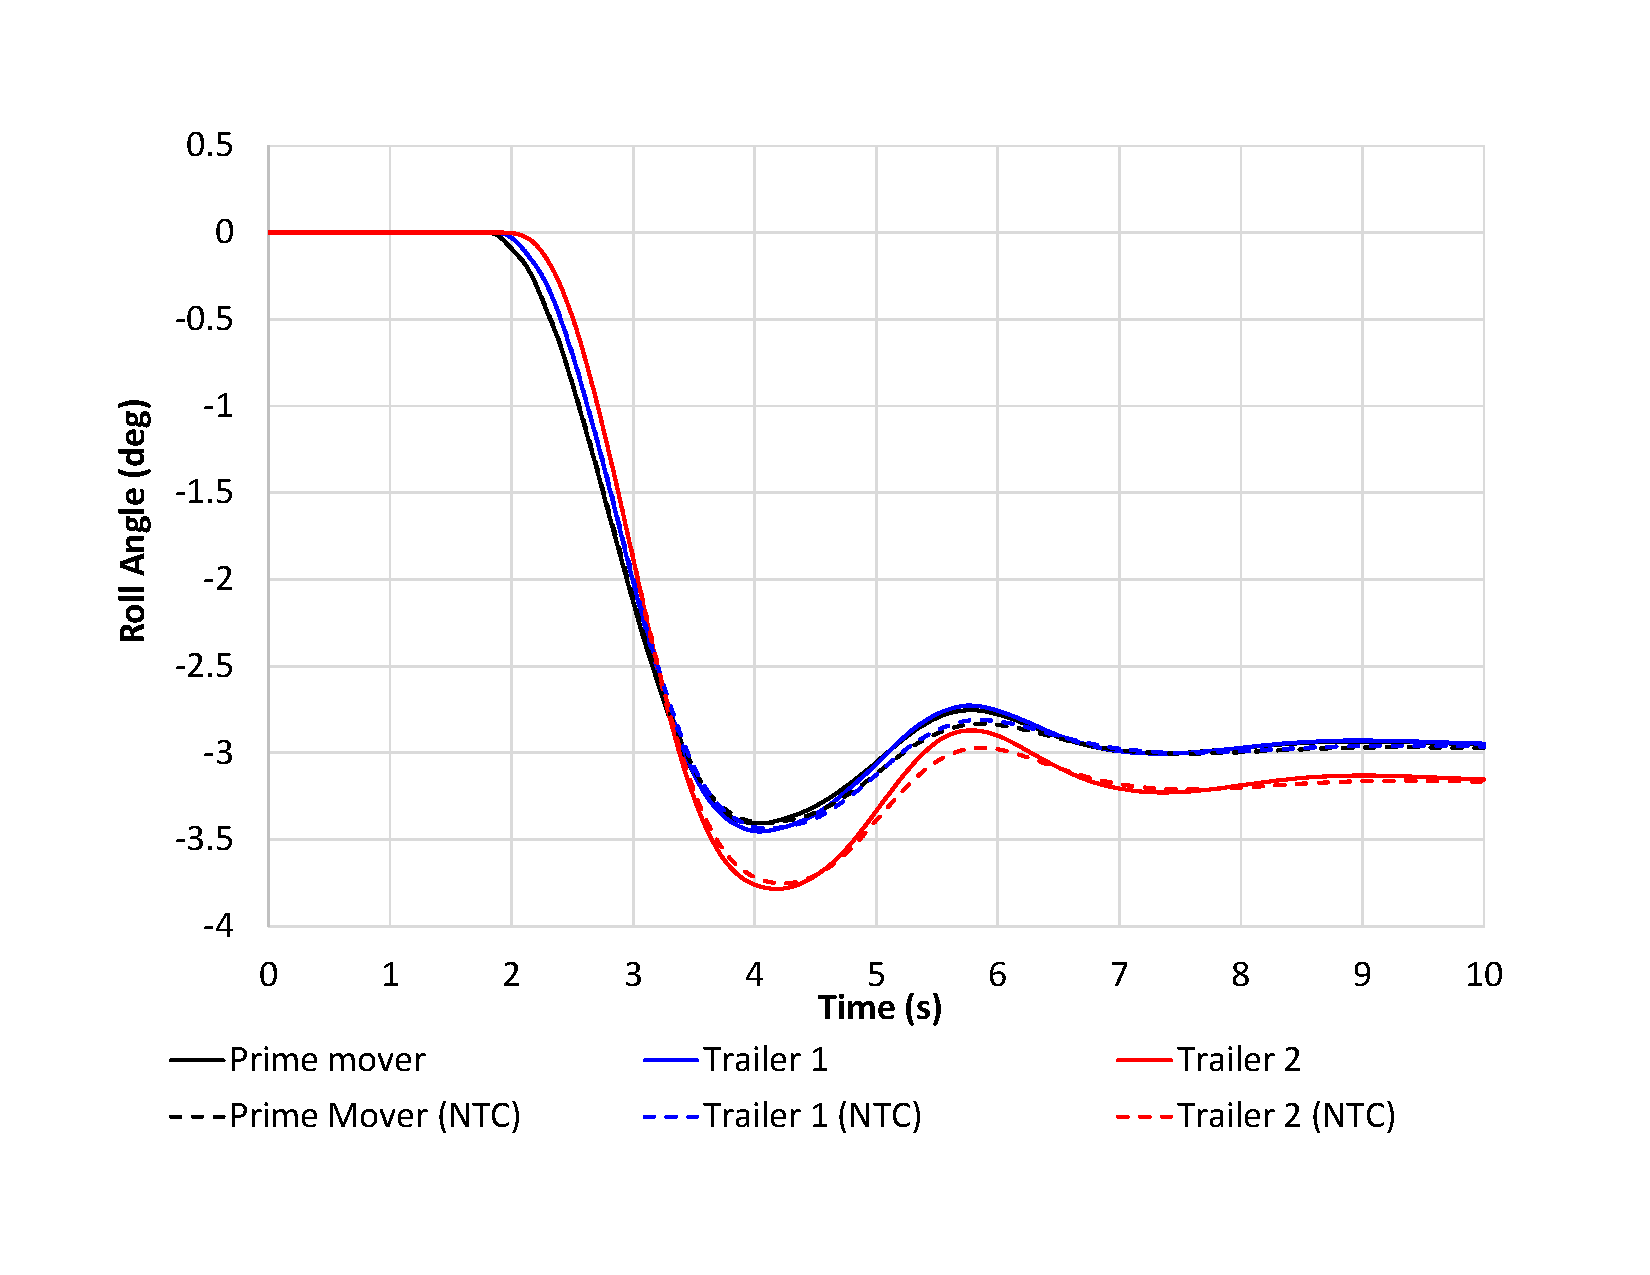
\includegraphics[width=0.8\textwidth]{fig/ntc-b-double_ssa}
        \caption{Roll angle from the B-double step steer simulations}
        \label{figure:ntc-b-double_ssa}
    \end{figure}
%----------------------------------------------
%      FIGURE
%----------------------------------------------

%----------------------------------------------
%      FIGURE
%----------------------------------------------
    \begin{figure}[H]
        \centering
        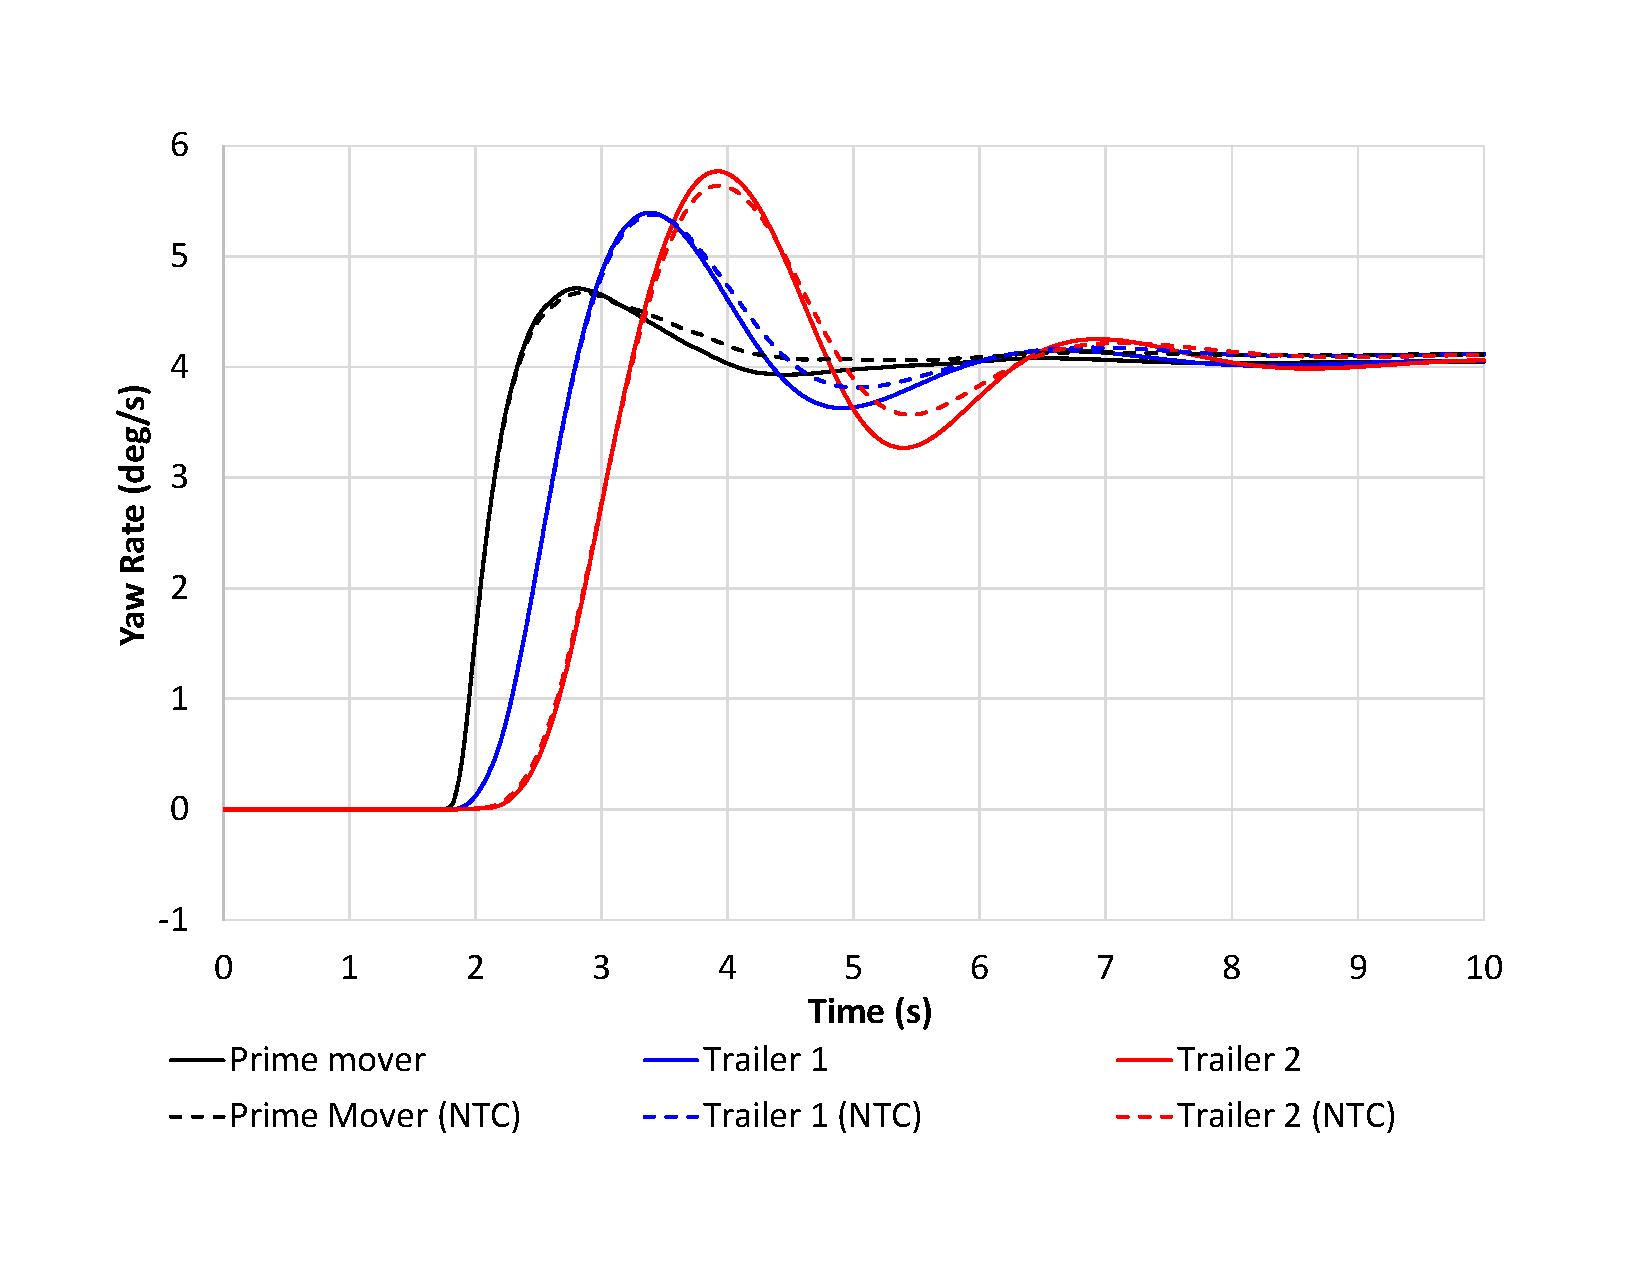
\includegraphics[width=0.8\textwidth]{fig/ntc-b-double_ssb}
        \caption{Yaw rates from the B-double step steer simulations}
        \label{figure:ntc-b-double_ssb}
    \end{figure}
%----------------------------------------------
%      FIGURE
%----------------------------------------------

%----------------------------------------------
%      FIGURE
%----------------------------------------------
    \begin{figure}[H]
        \centering
        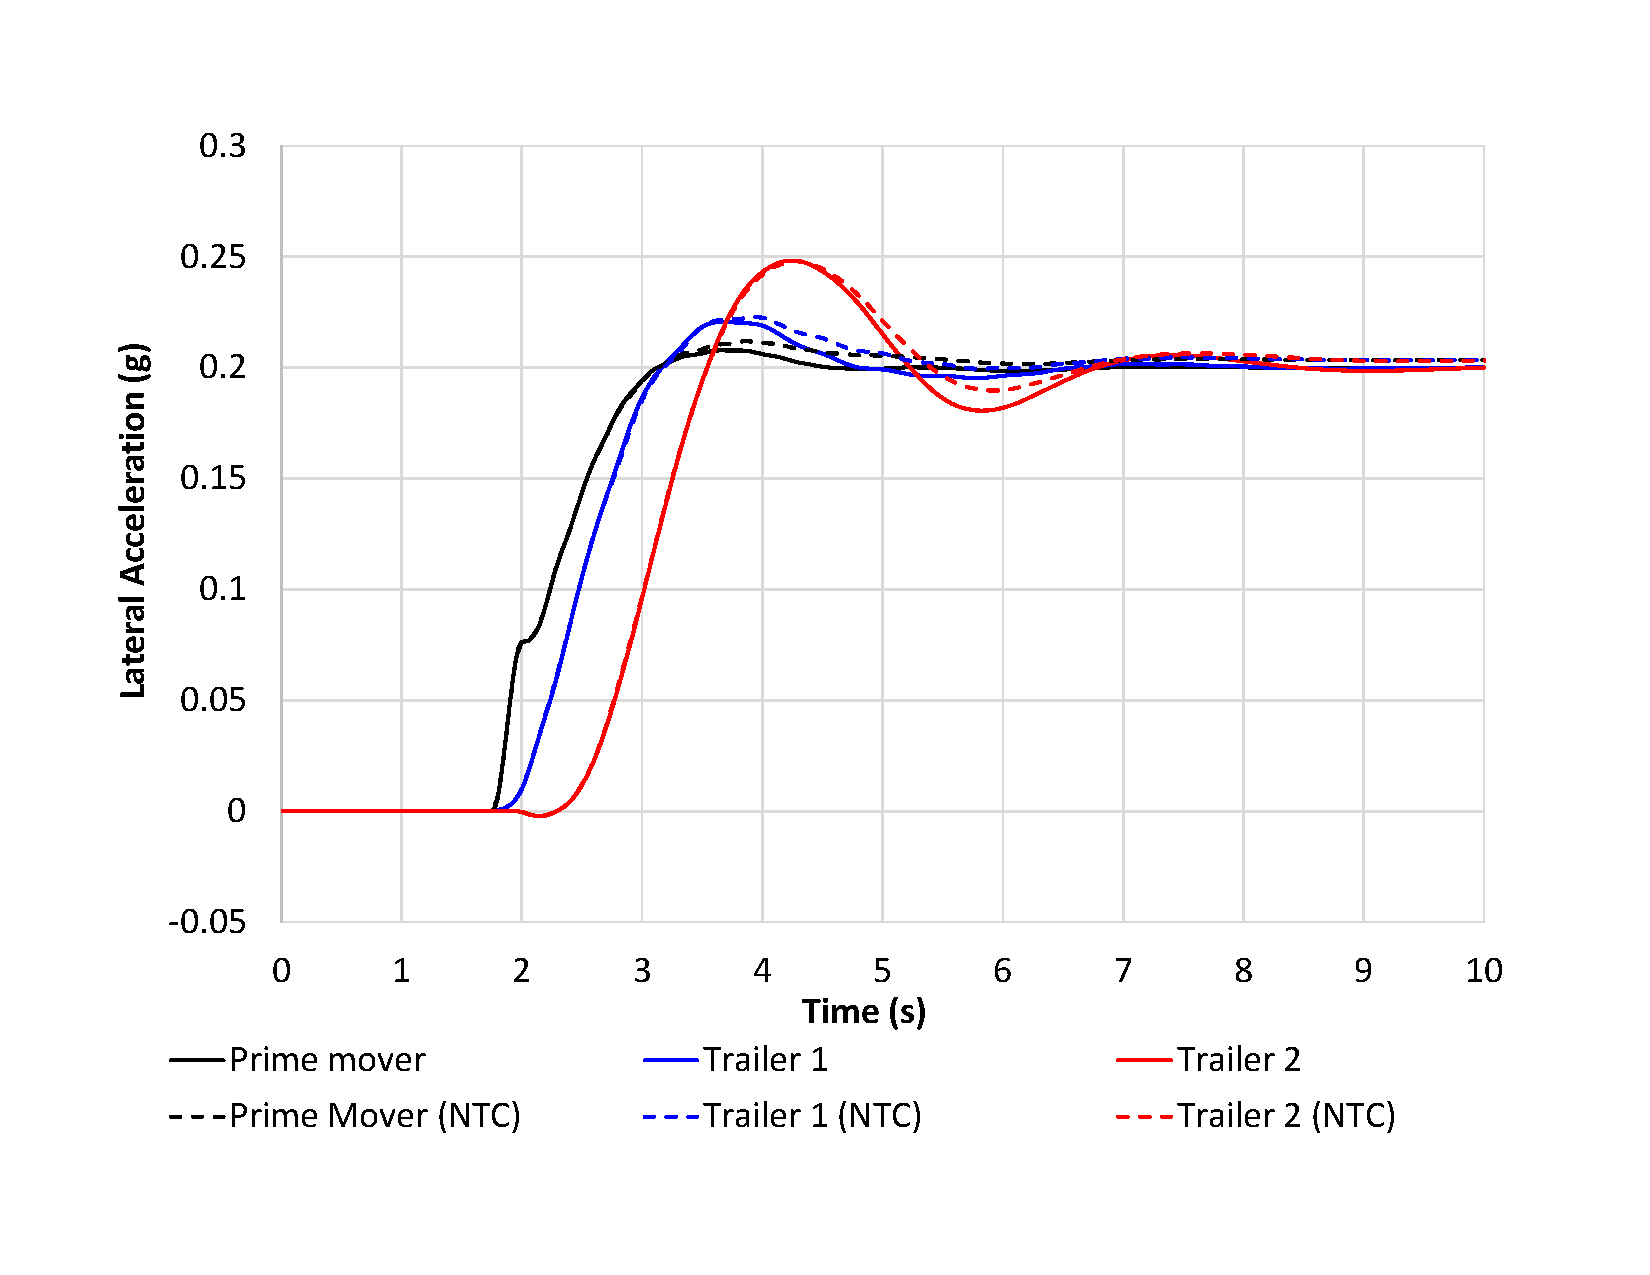
\includegraphics[width=0.8\textwidth]{fig/ntc-b-double_ssc}
        \caption{Lateral accelerations from the B-double step steer simulations}
        \label{figure:ntc-b-double_ssc}
    \end{figure}
%----------------------------------------------
%      FIGURE
%----------------------------------------------

%      SUBSECTION
%----------------------------------------------
\subsection{B-double Lane Change}\label{appendix:b-double-validation-lc}

%----------------------------------------------
%      FIGURE
%----------------------------------------------
    \begin{figure}[H]
        \centering
        \includegraphics[width=0.8\textwidth]{fig/ntc-b-double_lca}
        \caption{Steer axle lateral position from the B-double lane change simulations}
        \label{figure:ntc-b-double_lca}
    \end{figure}
%----------------------------------------------
%      FIGURE
%----------------------------------------------

%----------------------------------------------
%      FIGURE
%----------------------------------------------
    \begin{figure}[H]
        \centering
        \includegraphics[width=0.8\textwidth]{fig/ntc-b-double_lcb}
        \caption{Steer axle lateral position error from the B-double lane change simulations}
        \label{figure:ntc-b-double_lcb}
    \end{figure}
%----------------------------------------------
%      FIGURE
%----------------------------------------------

%----------------------------------------------
%      FIGURE
%----------------------------------------------
    \begin{figure}[H]
        \centering
        \includegraphics[width=0.8\textwidth]{fig/ntc-b-double_lcc}
        \caption{Yaw rates from the B-double lane change simulations}
        \label{figure:ntc-b-double_lcc}
    \end{figure}
%----------------------------------------------
%      FIGURE
%----------------------------------------------

%----------------------------------------------
%      FIGURE
%----------------------------------------------
    \begin{figure}[H]
        \centering
        \includegraphics[width=0.8\textwidth]{fig/ntc-b-double_lcd}
        \caption{Lateral accelerations from the B-double lane change simulations}
        \label{figure:ntc-b-double_lcd}
    \end{figure}
%----------------------------------------------
%      FIGURE
%----------------------------------------------

%      SUBSECTION
%----------------------------------------------
\subsection{B-double Low-speed 90\degree{} Turn}\label{appendix:b-double-validation-ls}

%----------------------------------------------
%      FIGURE
%----------------------------------------------
    \begin{figure}[H]
        \centering
        \includegraphics[width=0.8\textwidth]{fig/ntc-b-double_lsa}
        \caption{Trajectories from the B-double low-speed 90\degree{} turn simulations}
        \label{figure:ntc-b-double_lsa}
    \end{figure}
%----------------------------------------------
%      FIGURE
%----------------------------------------------

\section{Truck-trailer Validation}\label{appendix:NTC-truck-trailer-validation-results}

The NTC truck-trailer validation graphs are presented in Sections~\ref{appendix:truck-trailer-validation-ps}~to~\ref{appendix:truck-trailer-validation-ls}.


%      SUBSECTION
%----------------------------------------------
\subsection{Truck-trailer Pulse Steer}\label{appendix:truck-trailer-validation-ps}

%----------------------------------------------
%      FIGURE
%----------------------------------------------
\begin{figure}[H]
	\centering
	\includegraphics[width=0.8\textwidth]{fig/ntc-truck-trailer_psa}
	\caption{Tyre slip angles from the truck-trailer pulse steer simulations}
	\label{figure:ntc-truck-trailer_psa}
\end{figure}
%----------------------------------------------
%      FIGURE
%----------------------------------------------   

%----------------------------------------------
%      FIGURE
%----------------------------------------------
\begin{figure}[H]
	\centering
	\includegraphics[width=0.8\textwidth]{fig/ntc-truck-trailer_psb}
	\caption{Yaw rates from the truck-trailer pulse steer simulations}
	\label{figure:ntc-truck-trailer_psb}
\end{figure}
%----------------------------------------------
%      FIGURE
%----------------------------------------------

%----------------------------------------------
%      FIGURE
%----------------------------------------------
\begin{figure}[H]
	\centering
	\includegraphics[width=0.8\textwidth]{fig/ntc-truck-trailer_psc}
	\caption{Roll angles from the truck-trailer pulse steer simulations}
	\label{figure:ntc-truck-trailer_psc}
\end{figure}
%----------------------------------------------
%      FIGURE
%----------------------------------------------

%----------------------------------------------
%      FIGURE
%----------------------------------------------
\begin{figure}[H]
	\centering
	\includegraphics[width=0.8\textwidth]{fig/ntc-truck-trailer_psd}
	\caption{Articulation angles from the truck-trailer pulse steer simulations}
	\label{figure:ntc-truck-trailer_psd}
\end{figure}
%----------------------------------------------
%      FIGURE
%----------------------------------------------

%----------------------------------------------
%      FIGURE
%----------------------------------------------
\begin{figure}[H]
	\centering
	\includegraphics[width=0.8\textwidth]{fig/ntc-truck-trailer_pse}
	\caption{Turntable coupling roll moments from the truck-trailer pulse steer simulations}
	\label{figure:ntc-truck-trailer_pse}
\end{figure}
%----------------------------------------------
%      FIGURE
%----------------------------------------------

%----------------------------------------------
%      FIGURE
%----------------------------------------------
\begin{figure}[H]
	\centering
	\includegraphics[width=0.8\textwidth]{fig/ntc-truck-trailer_psf}
	\caption{Pin coupling lateral forces from the truck-trailer pulse steer simulations}
	\label{figure:ntc-truck-trailer_psf}
\end{figure}
%----------------------------------------------
%      FIGURE
%----------------------------------------------

%----------------------------------------------
%      FIGURE
%----------------------------------------------
\begin{figure}[H]
	\centering
	\includegraphics[width=0.8\textwidth]{fig/ntc-truck-trailer_psg}
	\caption{Lateral accelerations from the truck-trailer pulse steer simulations}
	\label{figure:ntc-truck-trailer_psg}
\end{figure}
%----------------------------------------------
%      FIGURE
%----------------------------------------------

%      SUBSECTION
%----------------------------------------------
\subsection{Truck-trailer Step Steer}\label{appendix:truck-trailer-validation-ss}

%----------------------------------------------
%      FIGURE
%----------------------------------------------
\begin{figure}[H]
	\centering
	\includegraphics[width=0.8\textwidth]{fig/ntc-truck-trailer_ssa}
	\caption{Roll angles from the truck-trailer step steer simulations}
	\label{figure:ntc-truck-trailer_ssa}
\end{figure}
%----------------------------------------------
%      FIGURE
%----------------------------------------------

%----------------------------------------------
%      FIGURE
%----------------------------------------------
\begin{figure}[H]
	\centering
	\includegraphics[width=0.8\textwidth]{fig/ntc-truck-trailer_ssb}
	\caption{Yaw rates from the truck-trailer step steer simulations}
	\label{figure:ntc-truck-trailer_ssb}
\end{figure}
%----------------------------------------------
%      FIGURE
%----------------------------------------------

%----------------------------------------------
%      FIGURE
%----------------------------------------------
\begin{figure}[H]
	\centering
	\includegraphics[width=0.8\textwidth]{fig/ntc-truck-trailer_ssc}
	\caption{Lateral accelerations from the truck-trailer step steer simulations}
	\label{figure:ntc-truck-trailer_ssc}
\end{figure}
%----------------------------------------------
%      FIGURE
%----------------------------------------------

%      SUBSECTION
%----------------------------------------------
\subsection{Truck-trailer SAE Lane Change}\label{appendix:truck-trailer-validation-lc}

%----------------------------------------------
%      FIGURE
%----------------------------------------------
\begin{figure}[H]
	\centering
	\includegraphics[width=0.8\textwidth]{fig/ntc-truck-trailer_lcc}
	\caption{Yaw rates from the truck-trailer SAE lane change simulations}
	\label{figure:ntc-truck-trailer_lcc}
\end{figure}
%----------------------------------------------
%      FIGURE
%----------------------------------------------

%----------------------------------------------
%      FIGURE
%----------------------------------------------
\begin{figure}[H]
	\centering
	\includegraphics[width=0.8\textwidth]{fig/ntc-truck-trailer_lcd}
	\caption{Lateral accelerations from the truck-trailer SAE lane change simulations}
	\label{figure:ntc-truck-trailer_lcd}
\end{figure}
%----------------------------------------------
%      FIGURE
%----------------------------------------------

%      SUBSECTION
%----------------------------------------------
\subsection{Truck-trailer Low-speed 90\degree{} Turn}\label{appendix:truck-trailer-validation-ls}

%----------------------------------------------
%      FIGURE
%----------------------------------------------
\begin{figure}[H]
	\centering
	\includegraphics[width=0.8\textwidth]{fig/ntc-truck-trailer_lsa}
	\caption{Trajectories from the truck-trailer low-speed 90\degree{} turn simulations}
	\label{figure:ntc-truck-trailer_lsa}
\end{figure}
%----------------------------------------------
%      FIGURE
%----------------------------------------------
\chapter{Manufacturer Data}\label{appendix:manufacturer-data}
The sections that follow contain data that has been consolidated from data books published from \glspl{oem} in the public domain. This data has been used in aid of determining reasonable ranges of design parameters where applicable in Section~\ref{chapter:parameter-range-selection}.

\section{BPW Rigid Axles}\label{section:bpw-rigid-axles-catalogue}
The data included in the BPW rigid axles catalogue has been consolidated into Tables~\ref{table:bpw-rigid-axles-with-300-mm-drum-brake}~to~\ref{table:bpw-rigid-axles-with-430-mm-disc-brake}.

%----------------------------------------------
%      TABLE
%----------------------------------------------
\begin{table}[H]
	\centering\footnotesize
	\begin{threeparttable}
	
	\begin{tabulary}{\textwidth}{lccccccccc}
	\toprule
    \multicolumn{1}{c}{\begin{sideways}\textbf{OEM Description}\end{sideways}} & \begin{sideways}\textbf{Permitted axle load up to 105 km/h (kg)}\end{sideways} & \begin{sideways}\textbf{Tyres}\end{sideways} & \begin{sideways}\textbf{Track width (SP) (mm)}\end{sideways} & \begin{sideways}\textbf{Spring centre (FM) (mm)}\end{sideways} & \begin{sideways}\textbf{Axle cross section (mm)}\end{sideways} & \begin{sideways}\textbf{Tyre size}\end{sideways} & \begin{sideways}\textbf{Tyre example}\end{sideways} & \begin{sideways}\textbf{Overall width (P) (mm)}\end{sideways} & \begin{sideways}\textbf{Axle weight (kg)}\end{sideways} \\
	\midrule
    NHSF 6410 & 6,400 & Single & 2010  & 1300  & 120   & 15"/17.5"/19.5" & 10 R152) & 2277  & 270 \\
    NHSF 6410 & 6,400 & Single & 2195  & 1500  & 120   & 15"/17.5"/19.5" & 10 R152) & 2462  & 278 \\
    NHZF 6410 & 6,400 & Twin  & 1830  & 980   & 120   & 15"/17.5"/19.5" & 215/75 R17.5 & 2317  & 266 \\
    NHZF 6410 & 6,400 & Twin  & 1950  & 1100  & 120   & 15"/17.5"/19.5" & 215/75 R17.5 & 2437  & 271 \\
    NHZF 9010 & 9000  & Twin  & 1830  & 980   & 120   & 15"/17.5"/19.5" & 235/75 R17.5 & 2365  & 285 \\
    NHZF 9010 & 9000  & Twin  & 1900  & 1100  & 120   & 15"/17.5"/19.5" & 235/75 R17.5 & 2435  & 287 \\
    NHZF 9010 & 9000  & Twin  & 1950  & 1100  & 120   & 15"/17.5"/19.5" & 235/75 R17.5 & 2485  & 289 \\
    NHZF 9010 & 9000  & Twin  & 1995  & 1100  & 120   & 15"/17.5"/19.5" & 235/75 R17.5 & 2530  & 316 \\
    NHZF 10010 & 10,000 & Twin  & 1830  & 980   & 120   & 15"/17.5"/19.5" & 235/75 R17.5 & 2365  & 294 \\
    NHZF 10010 & 10,000 & Twin  & 1880  & 980   & 120   & 15"/17.5"/19.5" & 235/75 R17.5 & 2415  & 297 \\
    NHZF 10010 & 10,000 & Twin  & 1880  & 1100  & 120   & 15"/17.5"/19.5" & 235/75 R17.5 & 2415  & 297 \\
    NHZF 10010 & 10,000 & Twin  & 1950  & 1100  & 120   & 15"/17.5"/19.5" & 235/75 R17.5 & 2485  & 302 \\
    NHZF 10010 & 10,000 & Twin  & 1995  & 1100  & 120   & 15"/17.5"/19.5" & 235/75 R17.5 & 2530  & 304 \\
    NHZF 12010 & 12000 & Twin  & 1830  & 980   & 120   & 15"/17.5"/19.5" & 235/75 R17.5 & 2365  & 308 \\
    NHZF 12010 & 12000 & Twin  & 1880  & 980   & 120   & 15"/17.5"/19.5" & 235/75 R17.5 & 2415  & 312 \\
    NHZF 12010 & 12000 & Twin  & 1950  & 1000  & 120   & 15"/17.5"/19.5" & 235/75 R17.5 & 2485  & 317 \\
    NHZF 12010 & 12000 & Twin  & 1950  & 1100  & 120   & 15"/17.5"/19.5" & 235/75 R17.5 & 2485  & 317 \\
    NHZF 12010 & 12000 & Twin  & 1995  & 1100  & 120   & 15"/17.5"/19.5" & 235/75 R17.5 & 2530  & 320 \\
	\bottomrule
	\end{tabulary}

	\caption{BPW rigid axles with 300~mm drum brake}
	\label{table:bpw-rigid-axles-with-300-mm-drum-brake}

	%\begin{tablenotes}
		%\item[1] %\tnote{1}
	%\end{tablenotes}

	\end{threeparttable}
\end{table}
%----------------------------------------------
%      TABLE
%----------------------------------------------

%----------------------------------------------
%      TABLE
%----------------------------------------------
\begin{table}[H]
	\centering\footnotesize
	\begin{threeparttable}
	
	\begin{tabulary}{\textwidth}{lccccccccc}
	\toprule
    \multicolumn{1}{c}{\begin{sideways}\textbf{OEM Description}\end{sideways}} & \multicolumn{1}{c}{\begin{sideways}\textbf{Permitted axle load up to 105 km/h (kg)}\end{sideways}} & \multicolumn{1}{c}{\begin{sideways}\textbf{Tyres}\end{sideways}} & \multicolumn{1}{c}{\begin{sideways}\textbf{Track width (SP) (mm)}\end{sideways}} & \multicolumn{1}{c}{\begin{sideways}\textbf{Spring centre (FM) (mm)}\end{sideways}} & \multicolumn{1}{c}{\begin{sideways}\textbf{Axle cross section (mm)}\end{sideways}} & \multicolumn{1}{c}{\begin{sideways}\textbf{Tyre size}\end{sideways}} & \multicolumn{1}{c}{\begin{sideways}\textbf{Tyre example}\end{sideways}} & \multicolumn{1}{c}{\begin{sideways}\textbf{Overall width (P) (mm)}\end{sideways}} & \multicolumn{1}{c}{\begin{sideways}\textbf{Axle weight (kg)}\end{sideways}} \\
	\midrule
    KHSF 9008 & 9000  & Single & 2045  & 1300  & 120 x 10 & 19.5" & 425/55 R19.5 & 2475  & 303 \\
    KHSF 9010/3 & 9000  & Single & 2040  & 1300  & 120 x 10 & 19.5" & 425/55 R19.5 & 2470  & 306 \\
    KHZF 9008 & 9000  & Twin  & 1835  & 980   & 120 x 10 & 19.5" & 265/70 R19.5 & 2420  & 295 \\
    KHSF 9008 & 9000  & Single & 1965  & 1200  & 120 x 10 & 19.5" & 425/55 R19.5 & 2395  & 300 \\
    KHSF 9008 & 9000  & Single & 2005  & 1250  & 120 x 10 & 19.5" & 425/55 R19.5 & 2435  & 301 \\
    KHZF 10008-15 & 10000 & Twin  & 1930  & 980   & 120 x 15 & 19.5" & 265/70 R19.5 & 2515  & 341 \\
    KHZF 11010-15 & 11000 & Twin  & 1830  & 980   & 120 x 15 & 19.5" & 265/70 R19.5 & 2415  & 326 \\
    KHZF 11008-15 & 11000 & Twin  & 1930  & 1100  & 120 x 15 & 19.5" & 265/70 R19.5 & 2515  & 340 \\
    KHZF 11010-15 & 11000 & Twin  & 1930  & 1100  & 120 x 15 & 19.5" & 265/70 R19.5 & 2515  & 331 \\
    KHZF 12008-15 & 12000 & Twin  & 1930  & 1100  & 120 x 15 & 19.5" & 285/70 R19.5 & 2530  & 342 \\
    KHZF 12010-15 & 12000 & Twin  & 1930  & 1100  & 120 x 15 & 19.5" & 285/70 R19.5 & 2530  & 336 \\
	\bottomrule
	\end{tabulary}

	\caption{BPW rigid axles with 360 mm drum brake}
	\label{table:bpw-rigid-axles-with-360-mm-drum-brake}

	%\begin{tablenotes}
		%\item[1] %\tnote{1}
	%\end{tablenotes}

	\end{threeparttable}
\end{table}
%----------------------------------------------
%      TABLE
%----------------------------------------------

%----------------------------------------------
%      TABLE
%----------------------------------------------
\begin{table}[H]
	\centering\footnotesize
	\begin{threeparttable}
	
	\begin{tabulary}{\textwidth}{lccccccccc}
	\toprule
    \multicolumn{1}{c}{\begin{sideways}\textbf{OEM Description}\end{sideways}} & \begin{sideways}\textbf{Permitted axle load up to 105 km/h (kg)}\end{sideways} & \begin{sideways}\textbf{Tyres}\end{sideways} & \begin{sideways}\textbf{Track width (SP) (mm)}\end{sideways} & \begin{sideways}\textbf{Spring centre (FM) (mm)}\end{sideways} & \begin{sideways}\textbf{Axle cross section (mm)}\end{sideways} & \begin{sideways}\textbf{Tyre size}\end{sideways} & \begin{sideways}\textbf{Tyre example}\end{sideways} & \begin{sideways}\textbf{Overall width (P) (mm)}\end{sideways} & \begin{sideways}\textbf{Axle weight (kg)}\end{sideways} \\
	\midrule
    HSF 6510 & 6500  & Single & 2040  & 1300  & 120 x 10 & 20"/22.5" & 10 R20 & 2335  & 280 \\
    HSF 6508 & 6500  & Single & 2045  & 1300  & 120 x 10 & 20"/22.5" & 10 R20 & 2340  & 278 \\
    HSF 9010 & 9000  & Single & 2040  & 1200  & 120 x 10 & 20"/22.5"/24" & 385/65 R22.5 & 2435  & 291 \\
    HSF 9010 & 9000  & Single & 2040  & 1300  & 120 x 10 & 20"/22.5"/24" & 385/65 R22.5 & 2435  & 291 \\
    HSF 9010 & 9000  & Single & 2040  & 1300  & 120 x 10 & 20"/22.5"/24" & 385/65 R22.5 & 2435  & 289 \\
    HSF 9010 & 9000  & Single & 2040  & 1300  & 120 x 10 & 20"/22.5"/24" & 385/65 R22.5 & 2435  & 288 \\
    HSF 9010 & 9000  & Single & 2095  & 1300  & 120 x 10 & 20"/22.5"/24" & 385/65 R22.5 & 2490  & 293 \\
    HSF 9010 & 9000  & Single & 2095  & 1300  & 120 x 10 & 20"/22.5"/24" & 385/65 R22.5 & 2490  & 292 \\
    HSF 9010 & 9000  & Single & 2140  & 1400  & 120 x 10 & 20"/22.5"/24" & 385/65 R22.5 & 2535  & 294 \\
    HSF 9010 & 9000  & Single & 2140  & 1400  & 120 x 10 & 20"/22.5"/24" & 385/65 R22.5 & 2535  & 295 \\
    HSF 9010 & 9000  & Single & 2040  & 1200  & 120 x 10 & 20"/22.5"/24" & 385/65 R22.5 & 2435  & 328 \\
    HSF 9010 & 9000  & Single & 2040  & 1300  & 120 x 10 & 20"/22.5"/24" & 385/65 R22.5 & 2435  & 328 \\
    HZF 9010-15 & 9000  & Twin  & 1820  & 900   & 120 x 15 & 20"/22.5"/24" & 10 R22.5 & 2385  & 313 \\
    HZF 9010-15 & 9000  & Twin  & 1820  & 980   & 120 x 15 & 20"/22.5"/24" & 10 R22.5 & 2385  & 313 \\
    HSF 10110-15 & 10000 & Single & 2040  & 1200  & 120 x 15 & 20"/22.5"/24" & 425/65 R22.5 & 2475  & 358 \\
    HSF 11010 & 11000 & Single & 2040  & 1300  & 150 x 10 & 20"/22.5"/24" & 445/65 R22.5 & 2505  & 353 \\
    HZF 11010 & 11000 & Twin  & 1820  & 900   & 150 x 10 & 20"/22.5"/24" & 11 R22.5 & 2425  & 352 \\
    HZF 11010 & 11000 & Twin  & 1820  & 980   & 150 x 10 & 20"/22.5"/24" & 11 R22.5 & 2425  & 352 \\
    HSF 12010 & 12000 & Single & 2040  & 1300  & 150 x 10 & 20"/22.5"/24" & 445/65 R22.5 & 2505  & 365 \\
    HZF 12010-16 & 12000 & Twin  & 1820  & 900   & 150 x 16 & 20"/22.5"/24" & 12 R22.5 & 2495  & 380 \\
    HZF 12010-16 & 12000 & Twin  & 1820  & 980   & 150 x 16 & 20"/22.5"/24" & 12 R22.5 & 2495  & 380 \\
    HZF 14010-1 & 14000 & Twin  & 1820  & 900   & 150 x 16 & 20"/22.5"/24" & 12 R20 & 2500  & 442 \\

	\bottomrule
	\end{tabulary}

	\caption{BPW rigid axles with 420 mm drum brake}
	\label{table:bpw-rigid-axles-with-420-mm-drum-brake}

	%\begin{tablenotes}
		%\item[1] %\tnote{1}
	%\end{tablenotes}

	\end{threeparttable}
\end{table}
%----------------------------------------------
%      TABLE
%----------------------------------------------

%----------------------------------------------
%      TABLE
%----------------------------------------------
\begin{table}[H]
	\centering\footnotesize
	\begin{threeparttable}
	
	\begin{tabulary}{\textwidth}{lccccccccc}
	\toprule
    \multicolumn{1}{c}{\begin{sideways}\textbf{OEM Description}\end{sideways}} & \begin{sideways}\textbf{Permitted axle load up to 105 km/h (kg)}\end{sideways} & \begin{sideways}\textbf{Tyres}\end{sideways} & \begin{sideways}\textbf{Track width (SP) (mm)}\end{sideways} & \begin{sideways}\textbf{Spring centre (FM) (mm)}\end{sideways} & \begin{sideways}\textbf{Axle cross section (mm)}\end{sideways} & \begin{sideways}\textbf{Tyre size}\end{sideways} & \begin{sideways}\textbf{Tyre example}\end{sideways} & \begin{sideways}\textbf{Overall width (P) (mm)}\end{sideways} & \begin{sideways}\textbf{Axle weight (kg)}\end{sideways} \\
	\midrule
    SKHBF 9010 & 9000  & Single & 2040  & 1300  & 120 x 10 & 22"   & 385/65 R22 & 2440  & 275 \\
    SKHBF 9010 & 9000  & Single & 2040  & 1200  & 120 x 10 & 22"   & 385/65 R22 & 2440  & 275 \\
    SKHBF 9010 & 9000  & Single & 2095  & 1300  & 120 x 10 & 22"   & 385/65 R22 & 2495  & 278 \\
    SKHBF 9010 & 9000  & Single & 2140  & 1400  & 120 x 10 & 22"   & 385/65 R22 & 2540  & 279 \\
    SKHSF 9008 & 9000  & Single & 2045  & 1300  & 120 x 10 & 19.5" & 425/55 R19.5 & 2470  & 254 \\
    SKHSF 9008 & 9000  & Single & 2045  & 1200  & 120 x 10 & 19.5" & 425/55 R19.5 & 2470  & 254 \\
    SKHSF 9010 & 9000  & Single & 2040  & 1300  & 120 x 10 & 22.5" & 385/65 R22.5 & 2440  & 265 \\
    SKHSF 9010 & 9000  & Single & 2040  & 1200  & 120 x 10 & 22.5" & 385/65 R22.5 & 2440  & 265 \\
    SKHSF 9010 & 9000  & Single & 2095  & 1300  & 120 x 10 & 22.5" & 385/65 R22.5 & 2495  & 268 \\
    SKHSF 9010 & 9000  & Single & 2140  & 1300  & 120 x 10 & 22.5" & 385/65 R22.5 & 2540  & 269 \\
    SKHSF 9010 & 9000  & Single & 2140  & 1400  & 120 x 10 & 22.5" & 385/65 R22.5 & 2540  & 269 \\
    SKHSF 9008 & 9000  & Single & 2005  & 1100  & 120 x 15 & 19.5" & 425/55 R19.5 & 2430  & 275 \\
    SKHSF 9010 & 9000  & Single & 2000  & 1100  & 120 x 15 & 22.5" & 385/65 R22.5 & 2400  & 286 \\
    SKHZF 9008 & 9000  & Twin  & 1885  & 980   & 120 x 15 & 19.5" & 265/70 R19.5 & 2465  & 270 \\
    SKHZF 9008 & 9000  & Twin  & 1925  & 980   & 120 x 15 & 19.5" & 265/70 R19.5 & 2505  & 272 \\
    SKHZF 9010 & 9000  & Twin  & 1880  & 980   & 120 x 15 & 22.5" & 10 R22.5 & 2425  & 280 \\
    SKHSF 10010 & 10000 & Single & 2040  & 1300  & 120 x 15 & 19.5" & 445/65 R19.5 & 2505  & 302 \\
    SKHZF 10008 & 10000 & Twin  & 1880  & 980   & 120 x 15 & 19.5" & 265/70 R19.5 & 2460  & 290 \\
    SKHZF 10008 & 10000 & Twin  & 1920  & 980   & 120 x 15 & 19.5" & 265/70 R19.5 & 2500  & 292 \\
    SKHZF 10008 & 10000 & Twin  & 1970  & 1100  & 120 x 15 & 19.5" & 265/70 R19.5 & 2550  & 294 \\
    SKHZF 10008 & 10000 & Twin  & 1920  & 1100  & 120 x 15 & 19.5" & 265/70 R19.5 & 2500  & 292 \\

	\bottomrule
	\end{tabulary}

	\caption{BPW rigid axles with 370 mm disc brake}
	\label{table:bpw-rigid-axles-with-370-mm-disc-brake}

	%\begin{tablenotes}
		%\item[1] %\tnote{1}
	%\end{tablenotes}

	\end{threeparttable}
\end{table}
%----------------------------------------------
%      TABLE
%----------------------------------------------

%----------------------------------------------
%      TABLE
%----------------------------------------------
\begin{table}[H]
	\centering\footnotesize
	\begin{threeparttable}
	
	\begin{tabulary}{\textwidth}{lccccccccc}
	\toprule
    \multicolumn{1}{c}{\begin{sideways}\textbf{OEM Description}\end{sideways}} & \begin{sideways}\textbf{Permitted axle load up to 105 km/h (kg)}\end{sideways} & \begin{sideways}\textbf{Tyres}\end{sideways} & \begin{sideways}\textbf{Track width (SP) (mm)}\end{sideways} & \begin{sideways}\textbf{Spring centre (FM) (mm)}\end{sideways} & \begin{sideways}\textbf{Axle cross section (mm)}\end{sideways} & \begin{sideways}\textbf{Tyre size}\end{sideways} & \begin{sideways}\textbf{Tyre example}\end{sideways} & \begin{sideways}\textbf{Overall width (P) (mm)}\end{sideways} & \begin{sideways}\textbf{Axle weight (kg)}\end{sideways} \\

	\midrule
    SHBF 9010 & 9000  & Single & 2040  & 1300  & 120 x 10 & 22.5" & 385/65 R22.5 & 2440  & 286 \\
    SHBF 9010 & 9000  & Single & 2040  & 1200  & 120 x 10 & 22.5" & 385/65 R22.5 & 2440  & 286 \\
    SHBF 9010 & 9000  & Single & 2095  & 1300  & 120 x 10 & 22.5" & 385/65 R22.5 & 2495  & 288 \\
    SHBF 9010 & 9000  & Single & 2140  & 1400  & 120 x 10 & 22.5" & 385/65 R22.5 & 2540  & 289 \\
    SHSF 9010 & 9000  & Single & 2040  & 1300  & 120 x 10 & 22.5" & 385/65 R22.5 & 2440  & 277 \\
    SHSF 9010 & 9000  & Single & 2040  & 1200  & 120 x 10 & 22.5" & 385/65 R22.5 & 2440  & 277 \\
    SHSF 9010 & 9000  & Single & 2095  & 1300  & 120 x 10 & 22.5" & 385/65 R22.5 & 2495  & 279 \\
    SHSF 9010 & 9000  & Single & 2140  & 1300  & 120 x 10 & 22.5" & 385/65 R22.5 & 2540  & 281 \\
    SHSF 9010 & 9000  & Single & 2140  & 1400  & 120 x 10 & 22.5" & 385/65 R22.5 & 2540  & 281 \\
    SHSF 9010 & 9000  & Single & 2040  & 1100  & 120 x 15 & 22.5" & 385/65 R22.5 & 2440  & 300 \\
    SHZF 9010 & 9000  & Twin  & 1880  & 980   & 120 x 15 & 22.5" & 10 R22.5 & 2450  & 292 \\
    SHSF 101102 & 10000 & Single & 2040  & 1200  & 120 x 15 & 22.5" & 425/65 R22.5 & 2480  & 317 \\
    SHSF 101102 & 10000 & Single & 2040  & 1300  & 120 x 15 & 22.5" & 425/65 R22.5 & 2480  & 317 \\
    SHZF 10110 & 10000 & Twin  & 1820  & 980   & 120 x 15 & 22.5" & 11 R22.5 & 2430  & 306 \\
    SHZF 10110 & 10000 & Twin  & 1850  & 980   & 120 x 15 & 22.5" & 11 R22.5 & 2460  & 308 \\
    SHZF 10110 & 10000 & Twin  & 1880  & 980   & 120 x 15 & 22.5" & 11 R22.5 & 2490  & 309 \\
    SHSF 12010 & 12000 & Single & 2040  & 1160  & 150 x 16 & 22.5" & 445/65 R22.5 & 2510  & 352 \\
    SHZF 12010 & 12000 & Twin  & 1820  & 900   & 150 x 16 & 22.5" & 12 R22.5 & 2460  & 339 \\
    SHZF 12010 & 12000 & Twin  & 1840  & 900   & 150 x 16 & 22.5" & 12 R22.5 & 2480  & 340 \\
    SHZF 12010 & 12000 & Twin  & 1880  & 980   & 150 x 16 & 22.5" & 12 R22.5 & 2520  & 343 \\

	\bottomrule
	\end{tabulary}

	\caption{BPW axles with 430 mm disc brake}
	\label{table:bpw-rigid-axles-with-430-mm-disc-brake}

	%\begin{tablenotes}
		%\item[1] %\tnote{1}
	%\end{tablenotes}

	\end{threeparttable}
\end{table}
%----------------------------------------------
%      TABLE
%----------------------------------------------

\section{Tyre Spring Rate}\label{section:tyre-spring-rate}
The \gls{oem} data for the tyre sizes used for the baseline combinations with calculated spring rates (assuming linear behaviour) is provided in Tables~\ref{table:spring-rate-approximation-for-445-65R22.5-tyres}~to~\ref{table:spring-rate-approximation-for-285/70 R19.5-tyres}.

%----------------------------------------------
%      TABLE
%----------------------------------------------
\begin{table}[H]
	\centering\footnotesize
	\begin{threeparttable}
	
	\begin{tabulary}{\textwidth}{rlccrcccrc}
	\toprule
             \multicolumn{1}{l}{\begin{sideways}\textbf{Manufacturer}\end{sideways}} & \begin{sideways}\textbf{Model}\end{sideways} & \begin{sideways}\textbf{Pressure (bar)}\end{sideways} & \begin{sideways}\textbf{Number of tyres}\end{sideways} & \multicolumn{1}{c}{\begin{sideways}\textbf{Axle load (kg)}\end{sideways}} & \begin{sideways}\textbf{Unladen radius (mm)}\end{sideways} & \begin{sideways}\textbf{Laden radius (mm)}\end{sideways} & \begin{sideways}\textbf{Load per tyre (kg)}\end{sideways} & \multicolumn{1}{c}{\begin{sideways}\textbf{Deflection (mm)}\end{sideways}} & \begin{sideways}\textbf{Spring rate (N/mm)}\end{sideways} \\
             \midrule
             \multicolumn{1}{l}{Bridgestone} & R244  & 9     & 2     & \multicolumn{1}{c}{11600} & 582   & 533   & 5800  & \multicolumn{1}{c}{48.26} & 1179 \\
             \multicolumn{1}{l}{Bridgestone} & M854  & 9     & 2     & \multicolumn{1}{c}{11600} & 583   & 536   & 5800  & \multicolumn{1}{c}{46.99} & 1211 \\
             \multicolumn{1}{l}{Bridgestone} & L315  & 8.3   & 2     & \multicolumn{1}{c}{11200} & 589   & 544   & 5600  & \multicolumn{1}{c}{45.72} & 1202 \\
             \multicolumn{1}{l}{Goodyear} & RHT/MST II & 5     & 2     & \multicolumn{1}{c}{7250} & 575   & 529   & 3625  & \multicolumn{1}{c}{46.00} & 773.1 \\
             \multicolumn{1}{l}{Goodyear} & RHT/MST II & 9     & 2     & \multicolumn{1}{c}{11600} & 575   & 529   & 5800  & \multicolumn{1}{c}{46.00} & 1237 \\
             \multicolumn{1}{l}{Michelin} & XZY TL & 7     & 2     & \multicolumn{1}{c}{9020} & 587   & 534   & 4510  & \multicolumn{1}{c}{53.00} & 834.8 \\
             \multicolumn{1}{l}{Michelin} & XZY TL & 9     & 2     & \multicolumn{1}{c}{11600} & 587   & 534   & 5800  & \multicolumn{1}{c}{53.00} & 1074 \\
             \midrule
                   &       &       &       & \textbf{Min. (mm)} & 575   &       &       & \textbf{Min. Singles (N/mm)} & 773.1 \\
                   &       &       &       & \textbf{Max. (mm)} & 589    &       &       & \textbf{Max. Singles (N/mm)} & 1237 \\
                   
	\bottomrule
	\end{tabulary}

	\caption{Spring rate approximation for 445/65 R22.5 tyres}
	\label{table:spring-rate-approximation-for-445-65R22.5-tyres}

	%\begin{tablenotes}
		%\item[1] %\tnote{1}
	%\end{tablenotes}

	\end{threeparttable}
\end{table}
%----------------------------------------------
%      TABLE
%----------------------------------------------

%----------------------------------------------
%      TABLE
%----------------------------------------------
\begin{table}[H]
	\centering\footnotesize
	\begin{threeparttable}
	
	\begin{tabulary}{\textwidth}{rlccccccrc}
	\toprule
             \multicolumn{1}{l}{\begin{sideways}\textbf{Manufacturer}\end{sideways}} & \begin{sideways}\textbf{Model}\end{sideways} & \begin{sideways}\textbf{Pressure (bar)}\end{sideways} & \begin{sideways}\textbf{Number of tyres}\end{sideways} & \begin{sideways}\textbf{Axle load (kg)}\end{sideways} & \begin{sideways}\textbf{Unladen radius (mm)}\end{sideways} & \begin{sideways}\textbf{Laden radius (mm)}\end{sideways} & \begin{sideways}\textbf{Load per tyre (kg)}\end{sideways} & \multicolumn{1}{c}{\begin{sideways}\textbf{Deflection (mm)}\end{sideways}} & \begin{sideways}\textbf{Spring rate (N/mm)}\end{sideways} \\
             \midrule
             \multicolumn{1}{l}{Bridgestone} & M860A & 9     & 2     & 9080  & 544   & 505   & 4540  & \multicolumn{1}{c}{38} & 1169 \\
             \multicolumn{1}{l}{Bridgestone} & M843  & 9     & 2     & 8250  & 550   & 511   & 4125  & \multicolumn{1}{c}{39} & 1028 \\
             \multicolumn{1}{l}{Goodyear} & LHS II+ & 5     & 2     & 5240  & 544   & 505   & 2620  & \multicolumn{1}{c}{38} & 674.6 \\
             \multicolumn{1}{l}{Goodyear} & LHS II+ & 8.5   & 2     & 8000  & 538   & 500   & 4000  & \multicolumn{1}{c}{38} & 1033 \\
             \multicolumn{1}{l}{Goodyear} & Ultragrip coach & 5     & 2     & 4910  & 544   & 505   & 2455  & \multicolumn{1}{c}{38} & 632.1 \\
             \multicolumn{1}{l}{Goodyear} & Ultragrip coach & 8.5   & 2     & 7500  & 538   & 500   & 3750  & \multicolumn{1}{c}{38} & 968.1 \\
             \multicolumn{1}{l}{Michelin} & XZA2 Energy TL & 6.5   & 2     & 6270  & 548   & 507   & 3135  & \multicolumn{1}{c}{41} & 750.1 \\
             \multicolumn{1}{l}{Michelin} & XZA2 Energy TL & 8     & 2     & 7500  & 548   & 507   & 3750  & \multicolumn{1}{c}{41} & 897.3 \\
             \multicolumn{1}{l}{Michelin} & XDY TL & 6.5   & 2     & 6270  & 548   & 506   & 3135  & \multicolumn{1}{c}{42} & 732.2 \\
             \multicolumn{1}{l}{Michelin} & XDY TL & 8     & 2     & 7500  & 548   & 506   & 3750  & \multicolumn{1}{c}{42} & 875.9 \\
             \multicolumn{1}{l}{Michelin} & Ice Grip TL & 6.5   & 2     & 6270  & 548   & 504   & 3135  & \multicolumn{1}{c}{44} & 699.0 \\
             \multicolumn{1}{l}{Michelin} & Ice Grip TL & 8     & 2     & 7570  & 548   & 504   & 3785  & \multicolumn{1}{c}{44} & 843.9 \\
             \multicolumn{1}{l}{Bridgestone} & M860A & 9     & 4     & 16480 & 544   & 505   & 4120  & \multicolumn{1}{c}{38} & 1061 \\
             \multicolumn{1}{l}{Bridgestone} & M843  & 9     & 4     & 15000 & 550   & 511   & 3750  & \multicolumn{1}{c}{39} & 934.4 \\
             \multicolumn{1}{l}{Goodyear} & RHD II+ & 5     & 4     & 8770  & 544   & 505   & 2193  & \multicolumn{1}{c}{38} & 564.5 \\
             \multicolumn{1}{l}{Goodyear} & RHD II+ & 8.5   & 4     & 13400 & 538   & 500   & 3350  & \multicolumn{1}{c}{38} & 864.8 \\
             \multicolumn{1}{l}{Goodyear} & MSS II & 5     & 4     & 8770  & 544   & 505   & 2193  & \multicolumn{1}{c}{38} & 564.5 \\
             \multicolumn{1}{l}{Goodyear} & MSS II & 8.5   & 4     & 13400 & 538   & 500   & 3350  & \multicolumn{1}{c}{38} & 864.8 \\
             \multicolumn{1}{l}{Michelin} & XZA2 Energy TL & 6.5   & 4     & 11090 & 548   & 507   & 2773  & \multicolumn{1}{c}{41} & 663.4 \\
             \multicolumn{1}{l}{Michelin} & XZA2 Energy TL & 8     & 4     & 13400 & 548   & 507   & 3350  & \multicolumn{1}{c}{41} & 801.5 \\
             \multicolumn{1}{l}{Michelin} & XDY TL & 6.5   & 4     & 11090 & 548   & 506   & 2773  & \multicolumn{1}{c}{42} & 647.6 \\
             \multicolumn{1}{l}{Michelin} & XDY TL & 8     & 4     & 13400 & 548   & 506   & 3350  & \multicolumn{1}{c}{42} & 782.5 \\
             \multicolumn{1}{l}{Michelin} & Ice Grip TL & 6.5   & 4     & 11090 & 548   & 504   & 2773  & \multicolumn{1}{c}{44} & 618.1 \\
             \multicolumn{1}{l}{Michelin} & Ice Grip TL & 8     & 4     & 13400 & 548   & 504   & 3350  & \multicolumn{1}{c}{44} & 746.9 \\
             \midrule
                   &       &       &       & \multicolumn{1}{r}{\textbf{Min. (mm)}} & 538   &       &       & \textbf{Min. Singles (N/mm)} & 632.1 \\
                   &       &       &       & \multicolumn{1}{r}{\textbf{Max. (mm)}} & 550   &       &       & \textbf{Max. Singles (N/mm)} & 1169 \\
                   &       &       &       &       &       &       &       & \textbf{Min. Duals (N/mm)} & 564.5 \\
                   &       &       &       &       &       &       &       & \textbf{Max. Duals (N/mm)} & 1061 \\

	\bottomrule
	\end{tabulary}
    
    
    

	\caption{Spring rate approximation for 315/80 R22.5 tyres}
	\label{table:Spring-rate-approximation-for-315-80R22.5-tyres}

	%\begin{tablenotes}
		%\item[1] %\tnote{1}
	%\end{tablenotes}

	\end{threeparttable}
\end{table}
%----------------------------------------------
%      TABLE
%----------------------------------------------

%----------------------------------------------
%      TABLE
%----------------------------------------------
\begin{table}[H]
	\centering\footnotesize
	\begin{threeparttable}
	
	\begin{tabulary}{\textwidth}{rlrrrrrrrc}
	\toprule
             \multicolumn{1}{l}{\begin{sideways}\textbf{Manufacturer}\end{sideways}} & \multicolumn{1}{c}{\begin{sideways}\textbf{Model}\end{sideways}} & \multicolumn{1}{c}{\begin{sideways}\textbf{Pressure (bar)}\end{sideways}} & \multicolumn{1}{c}{\begin{sideways}\textbf{Number of tyres}\end{sideways}} & \multicolumn{1}{c}{\begin{sideways}\textbf{Axle load (kg)}\end{sideways}} & \multicolumn{1}{c}{\begin{sideways}\textbf{Unladen radius (mm)}\end{sideways}} & \multicolumn{1}{c}{\begin{sideways}\textbf{Laden radius (mm)}\end{sideways}} & \multicolumn{1}{c}{\begin{sideways}\textbf{Load per tyre (kg)}\end{sideways}} & \multicolumn{1}{c}{\begin{sideways}\textbf{Deflection (mm)}\end{sideways}} & \begin{sideways}\textbf{Spring rate (N/mm)}\end{sideways} \\
             \midrule
             \multicolumn{1}{l}{Bridgestone} & \multicolumn{1}{l}{R227F} & \multicolumn{1}{c}{8.6} & \multicolumn{1}{c}{2} & \multicolumn{1}{c}{6300} & \multicolumn{1}{c}{448} & \multicolumn{1}{c}{414} & \multicolumn{1}{c}{3150} & \multicolumn{1}{c}{34.29} & 901.2 \\
             \multicolumn{1}{l}{Bridgestone} & \multicolumn{1}{l}{M729F} & \multicolumn{1}{c}{8.6} & \multicolumn{1}{c}{2} & \multicolumn{1}{c}{5800} & \multicolumn{1}{c}{450} & \multicolumn{1}{c}{414} & \multicolumn{1}{c}{2900} & \multicolumn{1}{c}{35.56} & 800.0 \\
             \multicolumn{1}{l}{Goodyear} & \multicolumn{1}{l}{RHT II} & \multicolumn{1}{c}{5} & \multicolumn{1}{c}{2} & \multicolumn{1}{c}{4190} & \multicolumn{1}{c}{448} & \multicolumn{1}{c}{408} & \multicolumn{1}{c}{2095} & \multicolumn{1}{c}{39.50} & 520.3 \\
             \multicolumn{1}{l}{Goodyear} & \multicolumn{1}{l}{RHT II} & \multicolumn{1}{c}{9} & \multicolumn{1}{c}{2} & \multicolumn{1}{c}{6700} & \multicolumn{1}{c}{448} & \multicolumn{1}{c}{408} & \multicolumn{1}{c}{3350} & \multicolumn{1}{c}{39.50} & 832.0 \\
             \multicolumn{1}{l}{Goodyear} & \multicolumn{1}{l}{RHS II} & \multicolumn{1}{c}{5} & \multicolumn{1}{c}{2} & \multicolumn{1}{c}{3750} & \multicolumn{1}{c}{448} & \multicolumn{1}{c}{413} & \multicolumn{1}{c}{1875} & \multicolumn{1}{c}{34.50} & 533.2 \\
             \multicolumn{1}{l}{Goodyear} & \multicolumn{1}{l}{RHS II} & \multicolumn{1}{c}{9} & \multicolumn{1}{c}{2} & \multicolumn{1}{c}{6000} & \multicolumn{1}{c}{448} & \multicolumn{1}{c}{413} & \multicolumn{1}{c}{3000} & \multicolumn{1}{c}{34.50} & 853.0 \\
             \multicolumn{1}{l}{Michelin} & \multicolumn{1}{l}{XZA TL} & \multicolumn{1}{c}{6} & \multicolumn{1}{c}{2} & \multicolumn{1}{c}{4320} & \multicolumn{1}{c}{456} & \multicolumn{1}{c}{413} & \multicolumn{1}{c}{2160} & \multicolumn{1}{c}{42.50} & 498.6 \\
             \multicolumn{1}{l}{Michelin} & \multicolumn{1}{l}{XZA TL} & \multicolumn{1}{c}{8} & \multicolumn{1}{c}{2} & \multicolumn{1}{c}{5800} & \multicolumn{1}{c}{456} & \multicolumn{1}{c}{413} & \multicolumn{1}{c}{2900} & \multicolumn{1}{c}{42.50} & 669.4 \\
             \multicolumn{1}{l}{Michelin} & \multicolumn{1}{l}{XTA TL} & \multicolumn{1}{c}{6.5} & \multicolumn{1}{c}{2} & \multicolumn{1}{c}{4940} & \multicolumn{1}{c}{456} & \multicolumn{1}{c}{409} & \multicolumn{1}{c}{2470} & \multicolumn{1}{c}{46.50} & 521.1 \\
             \multicolumn{1}{l}{Michelin} & \multicolumn{1}{l}{XTA TL} & \multicolumn{1}{c}{8.5} & \multicolumn{1}{c}{2} & \multicolumn{1}{c}{6300} & \multicolumn{1}{c}{456} & \multicolumn{1}{c}{409} & \multicolumn{1}{c}{3150} & \multicolumn{1}{c}{46.50} & 664.5 \\
             \multicolumn{1}{l}{Michelin} & \multicolumn{1}{l}{XTE2 TL} & \multicolumn{1}{c}{6.5} & \multicolumn{1}{c}{2} & \multicolumn{1}{c}{4900} & \multicolumn{1}{c}{456} & \multicolumn{1}{c}{409} & \multicolumn{1}{c}{2450} & \multicolumn{1}{c}{46.50} & 516.9 \\
             \multicolumn{1}{l}{Michelin} & \multicolumn{1}{l}{XTE2 TL} & \multicolumn{1}{c}{9} & \multicolumn{1}{c}{2} & \multicolumn{1}{c}{6700} & \multicolumn{1}{c}{456} & \multicolumn{1}{c}{409} & \multicolumn{1}{c}{3350} & \multicolumn{1}{c}{46.50} & 706.7 \\
             \multicolumn{1}{l}{Bridgestone} & \multicolumn{1}{l}{R227F} & \multicolumn{1}{c}{8.6} & \multicolumn{1}{c}{4} & \multicolumn{1}{c}{11600} & \multicolumn{1}{c}{448} & \multicolumn{1}{c}{414} & \multicolumn{1}{c}{2900} & \multicolumn{1}{c}{34.29} & 829.7 \\
             \multicolumn{1}{l}{Bridgestone} & \multicolumn{1}{l}{M729F} & \multicolumn{1}{c}{8.6} & \multicolumn{1}{c}{4} & \multicolumn{1}{c}{10900} & \multicolumn{1}{c}{450} & \multicolumn{1}{c}{414} & \multicolumn{1}{c}{2725} & \multicolumn{1}{c}{35.56} & 751.8 \\
             \multicolumn{1}{l}{Goodyear} & \multicolumn{1}{l}{RHT II} & \multicolumn{1}{c}{5} & \multicolumn{1}{c}{4} & \multicolumn{1}{c}{7880} & \multicolumn{1}{c}{448} & \multicolumn{1}{c}{408} & \multicolumn{1}{c}{1970} & \multicolumn{1}{c}{39.50} & 489.3 \\
             \multicolumn{1}{l}{Goodyear} & \multicolumn{1}{l}{RHT II} & \multicolumn{1}{c}{9} & \multicolumn{1}{c}{4} & \multicolumn{1}{c}{12600} & \multicolumn{1}{c}{448} & \multicolumn{1}{c}{408} & \multicolumn{1}{c}{3150} & \multicolumn{1}{c}{39.50} & 782.3 \\
             \multicolumn{1}{l}{Goodyear} & \multicolumn{1}{l}{RHS II} & \multicolumn{1}{c}{5} & \multicolumn{1}{c}{4} & \multicolumn{1}{c}{7000} & \multicolumn{1}{c}{448} & \multicolumn{1}{c}{413} & \multicolumn{1}{c}{1750} & \multicolumn{1}{c}{34.50} & 497.6 \\
             \multicolumn{1}{l}{Goodyear} & \multicolumn{1}{l}{RHS II} & \multicolumn{1}{c}{9} & \multicolumn{1}{c}{4} & \multicolumn{1}{c}{11200} & \multicolumn{1}{c}{448} & \multicolumn{1}{c}{413} & \multicolumn{1}{c}{2800} & \multicolumn{1}{c}{34.50} & 796.2 \\
             \multicolumn{1}{l}{Michelin} & \multicolumn{1}{l}{XZA TL} & \multicolumn{1}{c}{6} & \multicolumn{1}{c}{4} & \multicolumn{1}{c}{8200} & \multicolumn{1}{c}{456} & \multicolumn{1}{c}{413} & \multicolumn{1}{c}{2050} & \multicolumn{1}{c}{42.50} & 473.2 \\
             \multicolumn{1}{l}{Michelin} & \multicolumn{1}{l}{XZA TL} & \multicolumn{1}{c}{8} & \multicolumn{1}{c}{4} & \multicolumn{1}{c}{10900} & \multicolumn{1}{c}{456} & \multicolumn{1}{c}{413} & \multicolumn{1}{c}{2725} & \multicolumn{1}{c}{42.50} & 629.0 \\
             \multicolumn{1}{l}{Michelin} & \multicolumn{1}{l}{XTA TL} & \multicolumn{1}{c}{6.5} & \multicolumn{1}{c}{4} & \multicolumn{1}{c}{9090} & \multicolumn{1}{c}{456} & \multicolumn{1}{c}{409} & \multicolumn{1}{c}{2273} & \multicolumn{1}{c}{46.50} & 479.4 \\
             \multicolumn{1}{l}{Michelin} & \multicolumn{1}{l}{XTA TL} & \multicolumn{1}{c}{8.5} & \multicolumn{1}{c}{4} & \multicolumn{1}{c}{11600} & \multicolumn{1}{c}{456} & \multicolumn{1}{c}{409} & \multicolumn{1}{c}{2900} & \multicolumn{1}{c}{46.50} & 611.8 \\
             \multicolumn{1}{l}{Michelin} & \multicolumn{1}{l}{XTE2 TL} & \multicolumn{1}{c}{6.5} & \multicolumn{1}{c}{4} & \multicolumn{1}{c}{9000} & \multicolumn{1}{c}{456} & \multicolumn{1}{c}{409} & \multicolumn{1}{c}{2250} & \multicolumn{1}{c}{46.50} & 474.7 \\
             \multicolumn{1}{l}{Michelin} & \multicolumn{1}{l}{XTE2 TL} & \multicolumn{1}{c}{9} & \multicolumn{1}{c}{4} & \multicolumn{1}{c}{12300} & \multicolumn{1}{c}{456} & \multicolumn{1}{c}{409} & \multicolumn{1}{c}{3075} & \multicolumn{1}{c}{46.50} & 648.7 \\
             \midrule
                   &       &       &       & \textbf{Min. (mm)} & \multicolumn{1}{c}{448} &       & \textcolor[rgb]{ .439,  .188,  .627}{} & \textbf{Min Singles (N/mm)} & 498.6 \\
                   &       &       &       & \textbf{Max. (mm)} & \multicolumn{1}{c}{456} &       &       & \textbf{Max Singles (N/mm)} & 901.2 \\
                   &       &       &       &       &       &       &       & \textbf{Min Duals (N/mm)} & 473.2 \\
                   &       &       &       &       &       &       &       & \textbf{Max Duals (N/mm)} & 829.7 \\



	\bottomrule
	\end{tabulary}

	\caption{Spring rate approximation for 285/70 R19.5 tyres}
	\label{table:spring-rate-approximation-for-285/70 R19.5-tyres}

	%\begin{tablenotes}
		%\item[1] %\tnote{1}
	%\end{tablenotes}

	\end{threeparttable}
\end{table}
%----------------------------------------------
%      TABLE
%----------------------------------------------

\chapter{Anonymised PBS Data}\label{appendix:anonymised-pbs-data}
\section{Trailer and Dolly Units}\label{appendix:anonymised-pbs-data-trailer-and-dolly-units}
To gain insight into existing variations in design, data was extracted from South African \gls{pbs} assessments and anonymised for presentation in this research. The data extracted includes the wheelbase, sprung mass, \gls{cgz} as well as a normalised mass metric.

The normalised mass is calculated as the ratio of the sprung mass to the wheelbase in kg/m. The minimum  normalised mass was scaled with the baseline vehicles to determine a reasonable minimum for the sprung mass of the trailers used in the baselines considering a wide range of commodities transported in a combination of similar configuration. The normalised mass was calculated for the dolly using the ratio of the sprung mass to the axle spread.

%----------------------------------------------
%      TABLE
%----------------------------------------------
\begin{table}[H]
	\centering\footnotesize
	\begin{threeparttable}
	
	\begin{tabulary}{\textwidth}{lCCCC}
	\toprule
    \textbf{Trailer type} & \textbf{Wheelbase (m)} & \textbf{Sprung mass (kg)} & \textbf{\gls{cgz} (m)} & \textbf{(\gls{rsw}) (kg/m)} \\
	\midrule
    \multicolumn{1}{l}{Auger Bulker} & \multicolumn{1}{c}{9.440} & \multicolumn{1}{c}{7180} & 1.902 & 761 \\
    \multicolumn{1}{l}{Baseline tridem interlink follower} & \multicolumn{1}{c}{5.950} & \multicolumn{1}{c}{4167} & 1.912 & 700 \\
    \multicolumn{1}{l}{Baseline tridem interlink leader} & \multicolumn{1}{c}{7.420} & \multicolumn{1}{c}{4632} & 1.777 & 624 \\
    \multicolumn{1}{l}{Baseline quad semi-trailer} & \multicolumn{1}{c}{10.410} & \multicolumn{1}{c}{10410} & 2.025 & 1000 \\
    \multicolumn{1}{l}{Baseline tridem semi-trailer} & \multicolumn{1}{c}{8.255} & \multicolumn{1}{c}{3150} & 1.500 & 382 \\
    \multicolumn{1}{l}{Bottom dumper leader} & \multicolumn{1}{c}{8.850} & \multicolumn{1}{c}{5040} & 1.494 & 569 \\
    \multicolumn{1}{l}{Bottom dumper leader} & \multicolumn{1}{c}{8.100} & \multicolumn{1}{c}{4230} & 1.645 & 522 \\
    \multicolumn{1}{l}{Flat deck semi-trailer} & \multicolumn{1}{c}{5.400} & \multicolumn{1}{c}{3085} & 1.480 & 571 \\
    \multicolumn{1}{l}{Flat deck semi-trailer follower} & \multicolumn{1}{c}{5.530} & \multicolumn{1}{c}{3510} & 1.400 & 635 \\
    \multicolumn{1}{l}{Flat deck semi-trailer follower} & \multicolumn{1}{c}{7.329} & \multicolumn{1}{c}{3320} & 1.384 & 453 \\
    \multicolumn{1}{l}{Flat deck semi-trailer leader} & \multicolumn{1}{c}{7.590} & \multicolumn{1}{c}{4810} & 1.400 & 634 \\
    \multicolumn{1}{l}{Flat deck semi-trailer leader} & \multicolumn{1}{c}{6.670} & \multicolumn{1}{c}{2729} & 1.289 & 409 \\
    \multicolumn{1}{l}{Semi-trailer - timber} & \multicolumn{1}{c}{9.785} & \multicolumn{1}{c}{4965} & 1.300 & 507 \\
    \multicolumn{1}{l}{Semi-trailer - timber} & \multicolumn{1}{c}{12.600} & \multicolumn{1}{c}{3150} & 1.280 & 250 \\
    \multicolumn{1}{l}{Side tipper follower} & \multicolumn{1}{c}{5.200} & \multicolumn{1}{c}{4010} & 1.605 & 771 \\
    \multicolumn{1}{l}{Side tipper follower} & \multicolumn{1}{c}{5.200} & \multicolumn{1}{c}{4010} & 1.605 & 771 \\
    \multicolumn{1}{l}{Side tipper follower} & \multicolumn{1}{c}{5.950} & \multicolumn{1}{c}{4167} & 1.912 & 700 \\
    \multicolumn{1}{l}{Side tipper leader} & \multicolumn{1}{c}{8.250} & \multicolumn{1}{c}{4460} & 1.530 & 541 \\
    \multicolumn{1}{l}{Side tipper leader} & \multicolumn{1}{c}{8.250} & \multicolumn{1}{c}{4400} & 1.533 & 533 \\
    \multicolumn{1}{l}{Side tipper leader} & \multicolumn{1}{c}{8.250} & \multicolumn{1}{c}{4460} & 1.530 & 541 \\
    \multicolumn{1}{l}{Side tipper leader} & \multicolumn{1}{c}{7.420} & \multicolumn{1}{c}{4632} & 1.777 & 624 \\
    \multicolumn{1}{l}{Side tipper follower} & \multicolumn{1}{c}{5.350} & \multicolumn{1}{c}{3950} & 1.615 & 738 \\
    \multicolumn{1}{l}{Step-deck semi-trailer} & \multicolumn{1}{c}{7.175} & \multicolumn{1}{c}{4666} & 1.600 & 650 \\
    \multicolumn{1}{l}{Tanker - cement powder} & \multicolumn{1}{c}{8.770} & \multicolumn{1}{c}{4026} & 1.788 & 459 \\
    \multicolumn{1}{l}{Tanker - fuel} & \multicolumn{1}{c}{9.686} & \multicolumn{1}{c}{5212} & 1.324 & 538 \\
    \multicolumn{1}{l}{Tanker semi-trailer} & \multicolumn{1}{c}{9.686} & \multicolumn{1}{c}{5212} & 1.324 & 538 \\
    \multicolumn{1}{l}{Tautliner follower} & \multicolumn{1}{c}{8.200} & \multicolumn{1}{c}{3860} & 1.646 & 471 \\
    \multicolumn{1}{l}{Tautliner leader} & \multicolumn{1}{c}{9.085} & \multicolumn{1}{c}{4360} & 1.366 & 480 \\
    \multicolumn{1}{l}{Tautliner semi-trailer follower} & \multicolumn{1}{c}{6.478} & \multicolumn{1}{c}{3890} & 1.650 & 600 \\
    \multicolumn{1}{l}{Tautliner semi-trailer leader} & \multicolumn{1}{c}{7.960} & \multicolumn{1}{c}{3510} & 1.400 & 441 \\
    \multicolumn{1}{l}{Timber semi-trailer} & \multicolumn{1}{c}{8.255} & \multicolumn{1}{c}{3022} & 1.500 & 366 \\
    \midrule
    \multicolumn{3}{r}{\textbf{Minimum}} & 1.280 & 250 \\
    \multicolumn{3}{r}{\textbf{Maximum}} & 2.025 & 1000 \\

	\bottomrule
	\end{tabulary}

	\caption{Anonymised trailer \gls{cgz} and normalised sprung masses}
	\label{table:anonymised-trailer-centre-of-gravities-and-normalised-sprung-masses}

	%\begin{tablenotes}
		%\item[1] %\tnote{1}
	%\end{tablenotes}

	\end{threeparttable}
\end{table}
%----------------------------------------------
%      TABLE
%----------------------------------------------

%----------------------------------------------
%      TABLE
%----------------------------------------------
\begin{table}[H]
	\centering\footnotesize
	\begin{threeparttable}
	
	\begin{tabulary}{\textwidth}{lCCCC}
	\toprule
    \multicolumn{1}{l}{\textbf{Trailer type}} & \multicolumn{1}{c}{\textbf{Axle spread (m)}} & \multicolumn{1}{c}{\textbf{Sprung mass (kg)}} & \textbf{\gls{cgz} (m)} & (\gls{rsa}) \textbf{(kg/m)} \\
	\midrule
    \multicolumn{1}{l}{Baseline rigid drawbar  dolly} & \multicolumn{1}{c}{1.360} & \multicolumn{1}{c}{453} & 0.868 & 333 \\
    \multicolumn{1}{l}{Dolly} & \multicolumn{1}{c}{2.720} & \multicolumn{1}{c}{1435} & 1.000 & 528 \\
    \multicolumn{1}{l}{Dolly} & \multicolumn{1}{c}{2.720} & \multicolumn{1}{c}{800} & 1.050 & 294 \\
    \midrule
    \multicolumn{3}{r}{\textbf{Minimum}} & 0.868 & 294 \\
    \multicolumn{3}{r}{\textbf{Maximum}} & 1.050 & 528 \\

	\bottomrule
	\end{tabulary}

	\caption{Anonymised dolly \gls{cgz} and normalised sprung masses}
	\label{table:anonymised-dolly-centre-of-gravities-and-normalised-masses}

	%\begin{tablenotes}
		%\item[1] %\tnote{1}
	%\end{tablenotes}

	\end{threeparttable}
\end{table}
%----------------------------------------------
%      TABLE
%----------------------------------------------

\section{Prime Mover Units}\label{appendix:anonymised-pbs-data-vehicle-units}
A similar table was extracted for the prime mover units, using the wheelbase once again to normalise the sprung mass to find a reasonable minimum.

%----------------------------------------------
%      TABLE
%----------------------------------------------
\begin{table}[H]
	\centering\footnotesize
	\begin{threeparttable}
	
	\begin{tabulary}{\textwidth}{RRRRCC}
	\toprule
    \multicolumn{1}{l}{\textbf{Category}} & \multicolumn{1}{c}{\textbf{Axle arrangement}} & \multicolumn{1}{c}{\textbf{Wheelbase (m)}} & \multicolumn{1}{c}{\textbf{Sprung mass (kg)}} & \textbf{\gls{cgz} (mm)} & \gls{rsw} \textbf{(kg/m)}) \\
	\midrule
    \multicolumn{1}{l}{Baseline tractor} & \multicolumn{1}{c}{6x4} & \multicolumn{1}{c}{3.885} & \multicolumn{1}{c}{6598} & 1.204 & 1698 \\
    \multicolumn{1}{l}{Baseline rigid} & \multicolumn{1}{c}{6x4} & \multicolumn{1}{c}{5.285} & \multicolumn{1}{c}{6698} & 1.017 & 1267 \\
    \multicolumn{1}{l}{Tractor} & \multicolumn{1}{c}{6x4} & \multicolumn{1}{c}{3.975} & \multicolumn{1}{c}{5507} & 1.150 & 1385 \\
    \multicolumn{1}{l}{Tractor} & \multicolumn{1}{c}{6x4} & \multicolumn{1}{c}{3.9} & \multicolumn{1}{c}{4974} & 1.070 & 1275 \\
    \multicolumn{1}{l}{Tractor} & \multicolumn{1}{c}{6x4} & \multicolumn{1}{c}{3.975} & \multicolumn{1}{c}{5641} & 1.426 & 1419 \\
    \multicolumn{1}{l}{Tractor} & \multicolumn{1}{c}{6x4} & \multicolumn{1}{c}{3.975} & \multicolumn{1}{c}{5507} & 1.150 & 1385 \\
    \multicolumn{1}{l}{Tractor} & \multicolumn{1}{c}{6x4} & \multicolumn{1}{c}{3.9} & \multicolumn{1}{c}{4974} & 1.070 & 1275 \\
    \multicolumn{1}{l}{Tractor} & \multicolumn{1}{c}{6x4} & \multicolumn{1}{c}{3.885} & \multicolumn{1}{c}{5370} & 1.180 & 1382 \\
    \multicolumn{1}{l}{Tractor} & \multicolumn{1}{c}{6x4} & \multicolumn{1}{c}{3.885} & \multicolumn{1}{c}{6134} & 1.150 & 1579 \\
    \multicolumn{1}{l}{Tractor} & \multicolumn{1}{c}{6x4} & \multicolumn{1}{c}{3.885} & \multicolumn{1}{c}{5967} & 1.200 & 1536 \\
    \multicolumn{1}{l}{Tractor} & \multicolumn{1}{c}{6x4} & \multicolumn{1}{c}{3.885} & \multicolumn{1}{c}{6550} & 1.200 & 1686 \\
    \multicolumn{1}{l}{Tractor} & \multicolumn{1}{c}{6x4} & \multicolumn{1}{c}{3.975} & \multicolumn{1}{c}{5507} & 1.150 & 1385 \\
    \multicolumn{1}{l}{Tractor} & \multicolumn{1}{c}{6x4} & \multicolumn{1}{c}{3.9} & \multicolumn{1}{c}{5279} & 1.070 & 1354 \\
    \multicolumn{1}{l}{Tractor} & \multicolumn{1}{c}{6x4} & \multicolumn{1}{c}{3.9} & \multicolumn{1}{c}{4445} & 1.370 & 1140 \\
    \multicolumn{1}{l}{Rigid} & \multicolumn{1}{c}{6x4} & \multicolumn{1}{c}{5.285} & \multicolumn{1}{c}{5770} & 1.000 & 1092 \\
    \multicolumn{1}{l}{Rigid} & \multicolumn{1}{c}{6x4} & \multicolumn{1}{c}{5.2} & \multicolumn{1}{c}{4974} & 1.070 & 957 \\
    \multicolumn{1}{l}{Rigid} & \multicolumn{1}{c}{6x4} & \multicolumn{1}{c}{5.175} & \multicolumn{1}{c}{5655} & 1.008 & 1093 \\
    \multicolumn{1}{l}{Rigid} & \multicolumn{1}{c}{6x4} & \multicolumn{1}{c}{6.685} & \multicolumn{1}{c}{6030} & 1.315 & 902 \\
    \midrule
    \multicolumn{4}{r}{\textbf{Minimum (tractor)}} & 1.070 & 1140 \\
    \multicolumn{4}{r}{\textbf{Maximum (tractor)}} & 1.426 & 1698 \\
    \multicolumn{4}{r}{\textbf{Minimum (rigid)}} & 1.000 & 902 \\
    \multicolumn{4}{r}{\textbf{Maximum (rigid)}} & 1.315 & 1267 \\

	\bottomrule
	\end{tabulary}

	\caption{Anonymised prime mover \gls{cgz} and normalised sprung masses}
	\label{table:anonymised-prime-mover-cgz-and-normalised-sprung-masses}

	%\begin{tablenotes}
		%\item[1] %\tnote{1}
	%\end{tablenotes}

	\end{threeparttable}
\end{table}
%----------------------------------------------
%      TABLE
%----------------------------------------------
\end{document}
